% LaTeX source for ``Think Raku: How to Think Like a Computer Scientist''

% Copyright (c)  2017-2020  Laurent Rosenfeld, with Allen B. Downey.

% License: Creative Commons Attribution-NonCommercial 3.0 Unported License.
% http://creativecommons.org/licenses/by-nc/3.0/
%

%\documentclass[10pt,b5paper]{book}
\documentclass[10pt]{book}
\usepackage[width=5.5in,height=8.5in,
  hmarginratio=3:2,vmarginratio=1:1]{geometry}

% for some of these packages, you might have to install
% texlive-latex-extra (in Ubuntu)
 
\usepackage[T1]{fontenc}
\usepackage{textcomp}
\usepackage{mathpazo}
\usepackage{url}
\usepackage{fancyhdr}
\usepackage{graphicx}
\usepackage{amsmath}
\usepackage{amsthm}
%\usepackage{amssymb}
\usepackage{exercise}                   % texlive-latex-extra
\usepackage{makeidx}
%\usepackage{makeidx,showidx}
\usepackage{setspace}
\usepackage{hevea}                           
\usepackage{upquote}
\usepackage{appendix}
\usepackage[bookmarks]{hyperref}
\usepackage[english]{babel}
\usepackage[mathletters]{ucs}
\usepackage[utf8x]{inputenc}
\usepackage{fancyvrb}

%\usepackage{moreverb}

\title{Think Raku}
\author{Laurent Rosenfeld, with Allen B. Downey }
\newcommand{\thetitle}{Think Raku: How to Think Like a Computer Scientist}
\newcommand{\theversion}{2nd Edition, Version 0.6}
\newcommand{\thedate}{January 2020}

% these styles get translated in CSS for the HTML version
\newstyle{a:link}{color:black;}
\newstyle{p+p}{margin-top:1em;margin-bottom:1em}
\newstyle{img}{border:0px}

% define verbatim environment with a left margin
\DefineVerbatimEnvironment{verbatim}{Verbatim}{xleftmargin=.3in}

% change the arrows
\setlinkstext
  {\imgsrc[ALT="Previous"]{back.png}}
  {\imgsrc[ALT="Up"]{up.png}}
  {\imgsrc[ALT="Next"]{next.png}}

\setcounter{secnumdepth}{3}

\makeindex

\newif\ifplastex
\plastexfalse

\begin{document}


\frontmatter

% PLASTEX ONLY
\ifplastex
    \usepackage{localdef}
    \maketitle

\newcount\anchorcnt
\newcommand*{\Anchor}[1]{%
  \@bsphack%
    \Hy@GlobalStepCount\anchorcnt%
    \edef\@currentHref{anchor.\the\anchorcnt}% 
    \Hy@raisedlink{\hyper@anchorstart{\@currentHref}\hyper@anchorend}% 
    \M@gettitle{}\label{#1}% 
    \@esphack%
}


\else
% skip the following for plastex

\newtheorem{exercise}{Exercise}[chapter]

% LATEXONLY

% This file contains global declarations that latex2html doesn't want to
% see.  The latexonly environment doesn't work here because they need
% to have global scope.  latex2html ignores this style option completely
% as long as ``latexonly'' is listed in the $DONT_INCLUDE variable
% in the .latex2html-init file.

\sansfont{helvetica}
\typewriterfont{cmtt}

\newcommand{\bold}{\fontfamily{cmr}\series{bx}\shape{n}\size{12}{12pt}%
  \selectfont}
\newcommand{\smallfont}{\fontfamily{cmr}\series{m}\shape{n}\size{10}{11pt}%
  \selectfont}
\newcommand{\sem}{\fontfamily{cmr}\series{m}\shape{sl}\size{10}{11pt}%
  \selectfont}

\def\caps{\family{palatino}\size{12}{12pt}\selectfont}
\def\nintt{\family{helvetica}\size{9}{11pt}\selectfont}
\def\sanss{\family{helvetica}\size{11}{11pt}\selectfont}
\def\smalltt{\family{courier}\size{9}{11pt}\selectfont}

%
% bigverb is used to typeset verbatim text that is wide and needs to
% be typeset in a smaller font.  latex2html doesn't like the
% \verbatim command and has bigverb support hardcoded into it already,
% that's why it is here in latexonly.sty.
%
\newenvironment{bigverb}{\small\verbatim}{\endverbatim}

\makeatletter
\newcommand{\protspec}[2]{\addcontentsline{toc}{subsection}{#1}%
  \subsection*{NAME} #2}
\newcommand{\topic}[1]{\subsection*{#1}}
\makeatother


\begin{latexonly}

\renewcommand{\blankpage}{\thispagestyle{empty} \quad \newpage}

%\blankpage
%\blankpage

% TITLE PAGES FOR LATEX VERSION

%-half title--------------------------------------------------
\thispagestyle{empty}

\begin{flushright}
\vspace*{2.0in}

\begin{spacing}{3}
{\huge Think Raku}\\
{\Large How to Think Like a Computer Scientist}
\end{spacing}

\vspace{0.25in}

\theversion

\thedate

\vfill

\end{flushright}

%--verso------------------------------------------------------

\blankpage
\blankpage
%\clearemptydoublepage
%\pagebreak
%\thispagestyle{empty}
%\vspace*{6in}

%--title page--------------------------------------------------
\pagebreak
\thispagestyle{empty}

\begin{flushright}
\vspace*{2.0in}

\begin{spacing}{3}
{\huge Think Raku}\\
{\Large How to Think Like a Computer Scientist}
\end{spacing}

\vspace{0.25in}

\theversion

\thedate

\vspace{1in}


{\Large
Laurent Rosenfeld,
with Allen B. Downey\\
}


\vspace{0.5in}

{\Large Green Tea Press}

{\small Needham, Massachusetts}

%\includegraphics[width=1in]{figs/logo1.pdf}
\vfill

\end{flushright}


%--copyright--------------------------------------------------
\pagebreak
\thispagestyle{empty}

{\small
Copyright \copyright ~2017-2020 Allen Downey, Laurent Rosenfeld.


\vspace{0.2in}

\begin{flushleft}
Green Tea Press       \\
9 Washburn Ave        \\
Needham MA 02492
\end{flushleft}

Permission is granted to copy, distribute, and/or modify this document
under the terms of the Creative Commons Attribution-NonCommercial 3.0 Unported
License, which is available at \url{http://creativecommons.org/licenses/by-nc/3.0/}.

The original form of this book is \LaTeX\ source code.  Compiling this
\LaTeX\ source has the effect of generating a device-independent
representation of a textbook, which can be converted to other formats
and printed.

The \LaTeX\ source for this book is available from
\url{https://github.com/LaurentRosenfeld/think_raku/}

\vspace{0.2in}

} % end small

\end{latexonly}


% HTMLONLY

\begin{htmlonly}

% TITLE PAGE FOR HTML VERSION

{\Large \thetitle}

{\large Laurent Rosenfeld,
with Allen B. Downey}

\theversion

\thedate

\setcounter{chapter}{-1}

\end{htmlonly}

\fi
% END OF THE PART WE SKIP FOR PLASTEX

% 
\chapter{Preface}

Welcome to the art of computer programming and to the 
new Perl~6 language. This will probably be 
the first published books using Perl~6 (or one of the first), 
a powerful, expressive, malleable and highly extensible 
programming language. But this book is less 
about Perl~6, and more about learning 
how to write programs for computers. 

This book is intended for beginners and does not require 
any prior programming knowledge, but it is my hope 
that even those of you with programming experience will 
benefit from reading it.

\section*{The Aim of this Book}

This aim of this book is not primarily to teach Perl~6, 
but instead to teach the art 
of programming, using the Perl~6 language. After having 
completed this book, you should hopefully be able 
to write programs to solve relatively difficult problems in 
Perl~6, but my main aim is to teach computer science, software 
programming, and problem solving rather than solely to teach 
the Perl~6 language itself. 

This means that I will not cover every aspect of Perl~6, but 
only a (relatively large, but yet incomplete) subset of it. 
By no means is this book intended to be a reference on the 
language.

It is not possible to learn programming or to learn a new 
programming language by just reading a book; practicing 
is essential. This book contains a lot of exercises. You 
are strongly encouraged to make a real effort to do them. And, 
whether successful or not in solving the exercises, you 
should take a look at the solutions in the Appendix, 
as, very often, several solutions are suggested with further 
discussion on the subject and the issues involved. Sometimes, the solution 
section of the Appendix also introduces examples of topics 
that will be covered in the next chapter--and sometimes even 
things that are not covered elsewhere in the book. So, to get 
the most out the book, I suggest you try to solve the exercises 
as well as review the solutions and attempt them.

There are more than one thousand code examples in this book; 
study them, make sure to understand them, and run them. When 
possible, try to change them and see what happens. You're 
likely to learn a lot from this process.


\section*{The History of this Book}

In the course of the last three to four years, I  
have translated or adapted to French a number of tutorials 
and articles on Perl 6, and I've also written a few entirely 
new ones in French.~\footnote{See for example 
\url{http://perl.developpez.com/cours/\#TutorielsPerl6}.} 
Together, these documents represented by the end of 2015 
somewhere between 250 and 300 pages of material on Perl~6. 
By that time, I had 
probably made public more material on Perl~6 in French than 
all other authors taken together.

In late 2015, I began to feel that a Perl~6 document for beginners 
was something missing that I was willing to undertake. 
I looked around and found that it did not seem to 
exist in English either. I came to the idea that, after all, 
it might be more useful to write such a document initially 
in English, to give it a broader audience. I started contemplating 
writing a beginner introduction to Perl~6 
programming. My idea at the time was something like a 50- to 
70-page tutorial and I started to gather material and ideas 
in this direction.

Then, something happened that changed my plans.

In December 2015, friends of mine were contemplating translating 
into French Allen B. Downey's \emph{Think Python, Second Edition}\footnote{See \url{http://greenteapress.com/wp/think-python-2e/}.}. 
I had read an earlier edition of that book and fully supported 
the idea of translating it\footnote{I know, it's 
about Python, not Perl. But I don't believe in engaging 
in ``language wars'' and think that we all have to learn from 
other languages; to me, Perl's motto, ``there is more than 
one way to do it,'' also means that doing it in Python (or some 
other language) is truly an acceptable possibility.}. As it 
turned out, I ended up being a co-translator and the technical 
editor of the French translation of that book\footnote{See 
\url{http://allen-downey.developpez.com/livres/python/pensez-python/}.}.

While working on the French translation of Allen's Python book, 
the idea came to me that, rather than writing a tutorial on 
Perl~6, it might be more useful to make a ``Perl~6 translation'' 
of \emph{Think Python}. Since I was in contact with Allen in the context 
of the French translation, I suggested this to Allen, who 
warmly welcomed the idea. This is how I started to write this 
book late January 2016, just after having completed the 
work on the French translation of his Python book.

This book is thus largely derived on Allen's \emph{Think Python}, 
but adapted to Perl~6. As it happened, it is also much more 
than just a ``Perl~6 translation'' of Allen's book: with 
quite a lot of new material, it has become a brand new book, 
largely indebted to Allen's book, but yet a new book for which 
I take all responsibility. Any errors are mine, 
not Allen's.

My hope is that this will be useful to the Perl~6 community, and 
more broadly to the open source and general 
computer programming communities. In an interview with 
\emph{LinuxVoice} (July 2015), Larry Wall, the creator of Perl~6, 
said: ``We do think that Perl 6 will be learnable as a first language.''
Hopefully this book will contribute to making this happen. 

\section*{Acknowledgments}

I just don't know how I could thank Larry Wall to the level of 
gratitude that he deserves for having created Perl in the first 
place, and Perl~6 more recently. Be blessed for eternity, Larry, 
for all of that. 

And thank to you all of you who took part to this 
adventure (in no particular order), Tom, Damian, 
chromatic, Nathan, brian, Jan, Jarkko, John, Johan, Randall, 
Mark Jason, Ovid, Nick, Tim, Andy, Chip, Matt, Michael, Tatsuhiko, 
Dave, Rafael, Chris, Stevan, Saraty, Malcolm, Graham, Leon, 
Ricardo, Gurusamy, Scott and too many others to name.  

All my thanks also to those who believed in 
this Perl~6 project and made it happen, including those who 
quit at one point or another but contributed for some 
time; I know that this wasn't always easy.

Many thanks to Allen Downey, who very kindly supported my idea of 
adapting his book to Perl~6 and helped me in many respects, but 
also refrained from interfering in what I was putting into 
this new book.

I very warmly thank the people at O'Reilly who accepted the 
idea of this book and suggested many corrections or 
improvements. I want to thank especially 
Dawn Schanafelt, my editor at O'Reilly, whose advice 
has truly contributed to making this a better book. Many 
thanks also to Charles Roumeliotis, the copy editor, and 
Kristen Brown, the production editor, who fixed many 
typographical problems and spelling mistakes.

Thanks a lot in advance to readers who will offer comments 
or submit suggestions or corrections, as well as encouragements.

If you see anything that needs to be corrected or that 
could be improved, please kindly send your comments to 
\url{think.perl6 (at) gmail.com}.
% ...


\section*{Contributor List}

% ...
I would like to thank especially Moritz Lenz and Elizabeth 
Mattijsen, who reviewed in detail drafts of this book 
and suggested quite a number of improvements and corrections. Liz 
spent a lot of time on a detailed review of the full 
content of this book and I am especially grateful to her for 
her numerous and very useful comments. Thanks also to Timo Paulssen and 
ryanschoppe who also reviewed early drafts and provided some  
useful suggestions. Many thanks also to Uri Guttman, who reviewed 
this book and suggested a number of small corrections and improvements 
shortly before publication. 

Kamimura and James Lenz submitted a couple of  
corrections in the errata list on the O'Reilly web site.
zengargoyle pointed out a spurious character in a regex 
and fixed it in the GitHub repository of the book. Another 
James submitted an erratum on the O'Reilly web site.

\clearemptydoublepage

% TABLE OF CONTENTS
\begin{latexonly}

\tableofcontents

\clearemptydoublepage

\end{latexonly}



\chapter{Preface}

Welcome to the art of computer programming and to the 
new Perl~6 language. This will probably be 
the first published books using Perl~6 (or one of the first), 
a powerful, expressive, malleable and highly extensible 
programming language. But this book is less 
about Perl~6, and more about learning 
how to write programs for computers. 

This book is intended for beginners and does not require 
any prior programming knowledge, but it is my hope 
that even those of you with programming experience will 
benefit from reading it.

\section*{The Aim of this Book}

This aim of this book is not primarily to teach Perl~6, 
but instead to teach the art 
of programming, using the Perl~6 language. After having 
completed this book, you should hopefully be able 
to write programs to solve relatively difficult problems in 
Perl~6, but my main aim is to teach computer science, software 
programming, and problem solving rather than solely to teach 
the Perl~6 language itself. 

This means that I will not cover every aspect of Perl~6, but 
only a (relatively large, but yet incomplete) subset of it. 
By no means is this book intended to be a reference on the 
language.

It is not possible to learn programming or to learn a new 
programming language by just reading a book; practicing 
is essential. This book contains a lot of exercises. You 
are strongly encouraged to make a real effort to do them. And, 
whether successful or not in solving the exercises, you 
should take a look at the solutions in the Appendix, 
as, very often, several solutions are suggested with further 
discussion on the subject and the issues involved. Sometimes, the solution 
section of the Appendix also introduces examples of topics 
that will be covered in the next chapter--and sometimes even 
things that are not covered elsewhere in the book. So, to get 
the most out the book, I suggest you try to solve the exercises 
as well as review the solutions and attempt them.

There are more than one thousand code examples in this book; 
study them, make sure to understand them, and run them. When 
possible, try to change them and see what happens. You're 
likely to learn a lot from this process.


\section*{The History of this Book}

In the course of the last three to four years, I  
have translated or adapted to French a number of tutorials 
and articles on Perl 6, and I've also written a few entirely 
new ones in French.~\footnote{See for example 
\url{http://perl.developpez.com/cours/\#TutorielsPerl6}.} 
Together, these documents represented by the end of 2015 
somewhere between 250 and 300 pages of material on Perl~6. 
By that time, I had 
probably made public more material on Perl~6 in French than 
all other authors taken together.

In late 2015, I began to feel that a Perl~6 document for beginners 
was something missing that I was willing to undertake. 
I looked around and found that it did not seem to 
exist in English either. I came to the idea that, after all, 
it might be more useful to write such a document initially 
in English, to give it a broader audience. I started contemplating 
writing a beginner introduction to Perl~6 
programming. My idea at the time was something like a 50- to 
70-page tutorial and I started to gather material and ideas 
in this direction.

Then, something happened that changed my plans.

In December 2015, friends of mine were contemplating translating 
into French Allen B. Downey's \emph{Think Python, Second Edition}\footnote{See \url{http://greenteapress.com/wp/think-python-2e/}.}. 
I had read an earlier edition of that book and fully supported 
the idea of translating it\footnote{I know, it's 
about Python, not Perl. But I don't believe in engaging 
in ``language wars'' and think that we all have to learn from 
other languages; to me, Perl's motto, ``there is more than 
one way to do it,'' also means that doing it in Python (or some 
other language) is truly an acceptable possibility.}. As it 
turned out, I ended up being a co-translator and the technical 
editor of the French translation of that book\footnote{See 
\url{http://allen-downey.developpez.com/livres/python/pensez-python/}.}.

While working on the French translation of Allen's Python book, 
the idea came to me that, rather than writing a tutorial on 
Perl~6, it might be more useful to make a ``Perl~6 translation'' 
of \emph{Think Python}. Since I was in contact with Allen in the context 
of the French translation, I suggested this to Allen, who 
warmly welcomed the idea. This is how I started to write this 
book late January 2016, just after having completed the 
work on the French translation of his Python book.

This book is thus largely derived on Allen's \emph{Think Python}, 
but adapted to Perl~6. As it happened, it is also much more 
than just a ``Perl~6 translation'' of Allen's book: with 
quite a lot of new material, it has become a brand new book, 
largely indebted to Allen's book, but yet a new book for which 
I take all responsibility. Any errors are mine, 
not Allen's.

My hope is that this will be useful to the Perl~6 community, and 
more broadly to the open source and general 
computer programming communities. In an interview with 
\emph{LinuxVoice} (July 2015), Larry Wall, the creator of Perl~6, 
said: ``We do think that Perl 6 will be learnable as a first language.''
Hopefully this book will contribute to making this happen. 

\section*{Acknowledgments}

I just don't know how I could thank Larry Wall to the level of 
gratitude that he deserves for having created Perl in the first 
place, and Perl~6 more recently. Be blessed for eternity, Larry, 
for all of that. 

And thank to you all of you who took part to this 
adventure (in no particular order), Tom, Damian, 
chromatic, Nathan, brian, Jan, Jarkko, John, Johan, Randall, 
Mark Jason, Ovid, Nick, Tim, Andy, Chip, Matt, Michael, Tatsuhiko, 
Dave, Rafael, Chris, Stevan, Saraty, Malcolm, Graham, Leon, 
Ricardo, Gurusamy, Scott and too many others to name.  

All my thanks also to those who believed in 
this Perl~6 project and made it happen, including those who 
quit at one point or another but contributed for some 
time; I know that this wasn't always easy.

Many thanks to Allen Downey, who very kindly supported my idea of 
adapting his book to Perl~6 and helped me in many respects, but 
also refrained from interfering in what I was putting into 
this new book.

I very warmly thank the people at O'Reilly who accepted the 
idea of this book and suggested many corrections or 
improvements. I want to thank especially 
Dawn Schanafelt, my editor at O'Reilly, whose advice 
has truly contributed to making this a better book. Many 
thanks also to Charles Roumeliotis, the copy editor, and 
Kristen Brown, the production editor, who fixed many 
typographical problems and spelling mistakes.

Thanks a lot in advance to readers who will offer comments 
or submit suggestions or corrections, as well as encouragements.

If you see anything that needs to be corrected or that 
could be improved, please kindly send your comments to 
\url{think.perl6 (at) gmail.com}.
% ...


\section*{Contributor List}

% ...
I would like to thank especially Moritz Lenz and Elizabeth 
Mattijsen, who reviewed in detail drafts of this book 
and suggested quite a number of improvements and corrections. Liz 
spent a lot of time on a detailed review of the full 
content of this book and I am especially grateful to her for 
her numerous and very useful comments. Thanks also to Timo Paulssen and 
ryanschoppe who also reviewed early drafts and provided some  
useful suggestions. Many thanks also to Uri Guttman, who reviewed 
this book and suggested a number of small corrections and improvements 
shortly before publication. 

Kamimura and James Lenz submitted a couple of  
corrections in the errata list on the O'Reilly web site.
zengargoyle pointed out a spurious character in a regex 
and fixed it in the GitHub repository of the book. Another 
James submitted an erratum on the O'Reilly web site.

\clearemptydoublepage

% TABLE OF CONTENTS
\begin{latexonly}

\tableofcontents

\clearemptydoublepage

\end{latexonly}



% START THE BOOK
\mainmatter

\part{Starting with the Basics}

% intro_part_1.tex -- Introduction to first part of the book
%

This book has been divided in two parts. The main reason for that
is that I wanted to make a distinction between on the one hand 
relatively basic notions that are really needed for any programmer 
using Perl 6, and on the other hand more advanced concepts that 
a good programmer needs to know but may be less often needed in 
the day-to-day development work.

The first eleven chapters (a bit more than 200~pages) which make up 
this first part are meant to teach the concepts that every 
programmer should know: variables, expressions, statements, 
functions, conditionals, recursion, operator precedence, loops, etc., 
as well as the basic data structures commonly used, and the most 
useful algorithms.  These chapters can, I believe, be the basis 
for a one-semester introductory course on programming. 

Of course, the professor or teacher that wishes to use this 
material is entirely free to skip some details from this 
Part~1 (and also to include sections from Part~2), but, at 
least, I have provided some guidelines on how I think this 
book could be used to teach programming using the Perl~6 language.

The second part focuses on different programming paradigms and 
more advanced programming techniques that are in my opinion of 
paramount importance, but should probably studied in the context 
of a second, more advanced, semester.

For now, let's get down to the basics. It is my hope that you 
will enjoy the trip.



\chapter{The Way of the Program}

The goal of this book is to teach you to think like a computer
scientist.  This way of thinking combines some of the best features of
mathematics, engineering, and natural science.  Like mathematicians,
computer scientists use formal languages to denote ideas (specifically
computations).  Like engineers, they design things, assembling
components into systems and evaluating tradeoffs among alternatives.
Like scientists, they observe the behavior of complex systems, form
hypotheses, and test predictions.  
\index{problem solving}
\index{formal language}

The single most important skill for a computer scientist is {\bf
problem solving}.  Problem solving means the ability to formulate
problems, think creatively about solutions, and express a solution
clearly and accurately.  As it turns out, the process of learning to
program is an excellent opportunity to practice problem-solving
skills.  That's why this chapter is called, ``The Way of the
Program.''

On one level, you will be learning to program, a useful skill by
itself.  On another level, you will use programming as a means to an
end.  As we go along, that end will become clearer.
\index{programming}


\section{What is a Program?}

A {\bf program} is a sequence of instructions that specifies how to
perform a computation.  The computation might be something
mathematical, such as solving a system of equations or finding the
roots of a polynomial, but it can also be a symbolic computation, such
as searching and replacing text in a document, or something
graphical, like processing an image or playing a video.
\index{program}

The details look different in different languages, but a few basic
instructions appear in just about every language:

\begin{description}

\item[Input] Get data from the keyboard, a file, the network, 
a sensor, a GPS chip or some other device.
\index{input}

\item[Output] Display data on the screen, save it in a
file, send it over the network, act on a mechanical device,  etc.
\index{output}

\item[Math] Perform basic mathematical operations like addition and
multiplication.

\item[Conditional execution] Check for certain conditions and
run the appropriate code.
\index{conditional!execution}

\item[Repetition] Perform some action repeatedly, usually with
some variation.
\index{repetition}

\end{description}

Believe it or not, that's pretty much all there is to it.  Every
program you've ever used, no matter how complicated, is made up of
instructions that look pretty much like these.  So you can think of
programming as the process of breaking a large, complex task
into smaller and smaller subtasks until the subtasks are
simple enough to be performed with one of these basic instructions.
\index{instruction}

\index{abstraction}
\index{subtask}
Using or calling these subtasks makes it possible to create 
various levels of \emph{abstraction}. You have probably 
been told that computers only use 0's and 1's at the 
lowest level; but we usually don't have to worry about that. 
When we use a word processor to write a letter or a report, 
we are interested in files containing text and some 
formatting instructions, and with commands to change the 
file or to print it; fortunately, we don't have to care 
about the underlying 0's and 1's; the word-processing 
program offers us a much higher view (files, 
commands, etc.) that hides the gory underlying details.

Similarly, when we write a program, 
we usually use and/or create several layers of abstraction, 
so that, for example, once we have created a subtask that 
queries a database and stores the relevant data in 
memory, we no longer have to worry about the technical 
details of the subtask. We can use it as a sort of black 
box that will perform the desired operation for us. 
The essence of programming is to a very large extent this 
art of creating these successive layers of abstraction 
so that performing the higher level tasks becomes 
relatively easy.
\index{subtask}
\index{black box}


\section{Running Perl~6}
\label{running_perl_6}

One of the challenges of getting started with Perl~6 is that you
might have to install Perl~6 and related software on your computer. 
If you are familiar with your operating system, and especially
if you are comfortable with the shell or command-line interface, 
you will have no trouble installing Perl~6.  But for beginners, 
it can be painful to learn about system administration and 
programming at the same time.

To avoid that problem, you can start out running Perl~6 
in a web browser. You might want to use a search engine 
to find such a site. Currently, the easiest is probably 
to connect to the \url{https://glot.io/new/perl6} site, 
where you can type some Perl~6 code in the main window, run 
it, and see the result in the output window below.
\index{Perl~6 in a browser}

Sooner or later, however, you will really need to install 
Perl~6 on your computer.

The easiest way to install Perl~6 on your system is to 
download Rakudo Star (a distribution of Perl~6 that contains 
the Rakudo Perl~6 {\bf compiler}, documentation and useful modules): 
follow the instructions for your operating system at 
\url{http://rakudo.org/how-to-get-rakudo/} and at 
\url{https://perl6.org/downloads/}. 

\index{Perl 6 version}
As of this writing, the most recent specification of 
the language is Perl~6 version 6c (v6.c), and the most 
recent release available for download is Rakudo Star 2016.07; 
the examples in this book should 
all run with this version. You can find out the installed 
version by issuing the following command at the operating 
system prompt:
\begin{verbatim}
$ perl6 -v
This is Rakudo version 2016.07.1 built on MoarVM version 2016.07
implementing Perl 6.c.
\end{verbatim}

However, you should probably download and install the most recent 
version you can find. The output (warnings, error messages, 
etc.) you'll get from your version of Perl might in some 
cases slightly differ from what is printed in this book, 
but these possible differences should essentially be 
only cosmetic. 

Compared to Perl~5, Perl~6 is not just a new version of Perl. 
It is more like the new little sister of Perl~5. It does not 
aim at replacing Perl~5. Perl~6 is really a new programming language, 
with a syntax that is similar to earlier versions of 
Perl (such as Perl~5), but still markedly different. Unless 
stated otherwise, this book is about Perl~6 only, not about Perl~5 
and preceding versions of the Perl programming language. From now on, 
whenever we speak about \emph{Perl} with no further qualification, 
we mean Perl~6.

The Perl~6 {\bf interpreter} is a program that reads and 
executes Perl~6 code. It is sometimes called REPL (for ``read, 
evaluate, print, loop''). Depending on your environment, you 
might start the interpreter by clicking on an icon, or by 
typing {\tt perl6} on a command line.

When it starts, you should see output like this:
\index{interpreter}
\index{REPL}

\begin{verbatim}
To exit type 'exit' or '^D'
(Possibly some information about Perl and related software)
> 
\end{verbatim}
%

The last line with {\tt >} is a {\bf prompt} that indicates 
that the REPL is ready for you to enter code. If you type a 
line of code and hit Enter, the interpreter displays the
result: 
\index{prompt}

\begin{verbatim}
> 1 + 1
2
>
\end{verbatim}
%
You can type exit at the REPL prompt to exit the REPL.

Now you're ready to get started.
From here on, we assume that you know how to start the Perl~6
REPL and run code.


\section{The First Program}
\label{hello}
\index{Hello, World}

Traditionally, the first program you write in a new language
is called ``Hello, World'' because all it does is display the
words ``Hello, World.''  In Perl~6, it looks like this:

\begin{verbatim}
> say "Hello, World";
Hello, World
>
\end{verbatim}
%
\index{say function or method}
\index{function!say}
This is an example of what is usually called a {\bf print statement}, although it
doesn't actually print anything on paper and doesn't even 
use the {\tt print} keyword \footnote{Perl also has a {\tt print} 
function, but the {\tt say} built-in function is used here 
because it adds a new line character to the output.} (keywords are 
words which have a special meaning to the language and are 
used by the interpreter to recognize the structure of the program).  
The print statement displays a result on the screen.  In this case, 
the result is the words {\tt Hello, World}.
%
The quotation marks in the program indicate the beginning and end
of the text to be displayed; they don't appear in the result.
\index{quotation mark}
\index{print statement}
\index{statement!print}

The semi-colon ``{\tt ;}'' at the end of the line indicates 
that this is the end of the current statement. Although a 
semi-colon is technically not needed when running 
simple code directly under the REPL, it is usually 
necessary when writing a program with several lines of code, 
so you might as well just get into the habit of ending code 
instructions with a semi-colon.
\index{semi-colon}

Many other programming languages would require parentheses 
around the sentence to be displayed, but this is usually 
not necessary in Perl~6.

\section{Arithmetic Operators}
\index{operator!arithmetic}
\index{arithmetic operator}

After ``Hello, World,'' the next step is arithmetic.  Perl~6 provides
{\bf operators}, which are special symbols that represent computations
like addition and multiplication.  

The operators {\tt +}, {\tt -}, {\tt *}, and {\tt /} perform addition,
subtraction, multiplication and division, as in the following examples
under the REPL:

\begin{verbatim}
> 40 + 2
42
> 43 - 1
42
> 6 * 7
42
> 84 / 2
42
\end{verbatim}
%

Since we use the REPL, we don't need an explicit print 
statement in these examples, as the REPL automatically 
prints out the result of the statements for us. In a real 
program, you would need a print statement to display 
the result, as we'll see later. Similarly, if you run 
Perl statements in the web browser mentioned in 
Section~\ref{running_perl_6}, you will need a 
print statement to display the result of these operations. 
For example:

\begin{verbatim}
say 40 + 2;   # -> 42
\end{verbatim}


Finally, the operator {\tt **} performs exponentiation; that is,
it raises a number to a power:

\begin{verbatim}
> 6**2 + 6
42
\end{verbatim}
%
In some other languages, the caret (``\verb"^"'') or 
circumflex accent is used for exponentiation, but in 
Perl~6 it is used for some other purposes.
%
\index{set}
\index{set!operator}
\index{operator!set}


\section{Values and Types}
\label{values_and_types}
\index{value}
\index{type}
\index{string}

A {\bf value} is one of the basic things a program works with, like a
letter or a number.  Some values we have seen so far are {\tt 2},
{\tt 42}, and \verb'"Hello, World"'.

These values belong to different {\bf types}:
{\tt 2} is an {\bf integer}, {\tt 40 + 2} is also an integer, 
{\tt 84/2} is a {\bf rational number},
and \verb"'Hello, World'" is a {\bf string}, so called 
because the characters it contains are strung together.
\index{integer}
\index{floating-point}

If you are not sure what type a value has, Perl can
tell you:

\begin{verbatim}
> say 42.WHAT;
(Int)
> say (40 + 2).WHAT;
(Int)
> say (84 / 2).WHAT;
(Rat)
> say (42.0).WHAT
(Rat)
> say ("Hello, World").WHAT;
(Str)
>
\end{verbatim}
%
In these instructions, {\tt .WHAT} is known as an 
introspection method, that is a kind of method which 
will tell you \emph{what} (of  which type) the preceding 
expression is. {\tt 42.WHAT} is an example of the dot 
syntax used for method invocation: it calls the {\tt .WHAT} 
built-in on the ``42'' expression (the invocant) and provides 
to the {\tt say} function the result of this invocation, 
which in this case is the type of the expression.
\index{WHAT}
\index{introspection}
\index{string!type}
\index{type!Str}
\index{Int type}
\index{type!Int}
\index{rational!type}
\index{type!Rat}
\index{invocant}
\index{invocation}

Not surprisingly, integers belong to the type {\tt Int},
strings belong to {\tt Str} and rational 
numbers belong to {\tt Rat}.  

Although {\tt 40 + 2} and {\tt 84 / 2} seem to yield the 
same result (42), the first expression returns an integer 
({\tt Int}) and the second a rational number ({\tt Rat}). 
The number 42.0 is also a rational.

The rational type is somewhat uncommon in most programming 
languages. Internally, these numbers are stored as two 
integers representing the numerator and the denominator 
(in their simplest terms). For example, the number 17.3 
might be stored as two integers, 173 and 10, meaning that 
Perl is really storing something meaning the $\frac{173}{10}$ 
fraction. Although this is usually not needed (except 
for introspection or debugging), you might access these 
two integers with the following methods:

\begin{verbatim}
> my $num = 17.3;
17.3
> say $num.WHAT;
(Rat)
> say $num.numerator, " ", $num.denominator; # say can print a list
173 10
> say $num.nude;      # "nude" stands for numerator-denominator
(173 10) 
\end{verbatim}
\index{numerator method}
\index{method!numerator}
\index{denominator method}
\index{method!denominator}
\index{nude method}
\index{method!nude}
%
This may seem anecdotal, but, for reasons which are 
beyond the scope of this book, this makes it possible for Perl~6 
to perform arithmetical operations on rational numbers with 
a much higher accuracy than most common programming languages. 
For example, if you try to perform the arithmetical operation
\verb'0.3 - 0.2 - 0.1', with most general purpose programming languages 
(and depending on your machine architecture), you 
might obtain a result such as -2.77555756156289e-17 (in Perl~5), 
-2.775558e-17 (in C under gcc), or -2.7755575615628914e-17 
(Java, Python~3, Ruby, TCL). Don't worry about these values if you 
don't understand them, let us just say that they  are 
extremely small, but they are not 0, whereas,  
obviously, the result should really be zero. In Perl~6, 
the result is 0 (even to the fiftieth decimal digit):
\begin{verbatim}
> my $result-should-be-zero = 0.3 - 0.2 - 0.1;
0
> printf "%.50f", $result-should-be-zero; # prints 50 decimal digits
0.00000000000000000000000000000000000000000000000000
\end{verbatim}
%
In Perl~6, you might even compare the result of the operation with 0:
\begin{verbatim}
> say $result-should-be-zero == 0;
True
\end{verbatim}
%
Don't do such a comparison with most common programming 
languages; you're very likely to get a wrong result.

What about values like \verb'"2"' and \verb'"42.0"'?
They look like numbers, but they are in quotation marks like
strings.
\index{quotation mark}

\begin{verbatim}
> say '2'.perl; # perl returns a Perlish representation of the invocant
"2"
> say "2".WHAT;
(Str)
> say '42'.WHAT;
(Str)
\end{verbatim}
%
\index{invocant}

They're strings because they are defined within quotes. Although 
Perl will often perform the necessary conversions for you, it 
is generally a good practice not to use quotation marks if your value 
is intended to be a number.

When you type a large integer, you might be tempted to use commas
between groups of digits, as in {\tt 1,234,567}.  This is not a
legal {\em integer} in Perl~6, but it is a legal expression:

\begin{verbatim}
> 1,234,567
(1 234 567)
>
\end{verbatim}
%
That's actually a list of three different integer numbers, and 
not what we expected at all! 

\begin{verbatim}
> say (1,234,567).WHAT
(List)
\end{verbatim}

Perl~6 interprets {\tt 1,234,567} as a comma-separated 
sequence of three integers.  As we will see later, 
the comma is a separator used for constructing lists.
\index{comma}

You can, however, separate groups of digits with the underscore character ``\verb"_"'' for better legibility and obtain a 
proper integer:
\index{underscore character}

\begin{verbatim}
> 1_234_567
1234567
> say 1_234_567.WHAT
(Int)
>
\end{verbatim}
%

\index{sequence}



\section{Formal and Natural Languages}
\index{formal language}
\index{natural language}
\index{language!formal}
\index{language!natural}

{\bf Natural languages} are the languages people speak,
such as English, Spanish, and French.  They were not designed
by people (although people try to impose some order on them);
they evolved naturally.

{\bf Formal languages} are languages that are designed by people for
specific applications.  For example, the notation that mathematicians
use is a formal language that is particularly good at denoting
relationships among numbers and symbols.  Chemists use a formal
language to represent the chemical structure of molecules.  And
most importantly:

\begin{quote}
{\bf Programming languages are formal languages that have been
designed to express computations.}
\end{quote}

Formal languages tend to have strict {\bf syntax} rules that
govern the structure of statements.
For example, in mathematics the statement
$3 + 3 = 6$ has correct syntax, but
not $3 + = 3 \$ 6$.  In chemistry
$H_2O$ is a syntactically correct formula, but $_2Zz$ is not.
\index{syntax}

Syntax rules come in two flavors, pertaining to {\bf tokens} and
{\bf structure}.  Tokens are the basic elements of the language, such as
words, numbers, and chemical elements.  One of the problems with
$3 += 3 \$ 6$ is that \( \$ \) is not a legal token in mathematics
(at least as far as I know).  Similarly, $_2Zz$ is not legal because
there is no chemical element with the abbreviation $Zz$.
\index{token}
\index{structure}

The second type of syntax rule, structure, pertains to the way tokens are
combined.  The equation $3 += 3$ is illegal in mathematics 
because even though $+$ and $=$ are legal tokens, you can't 
have one right after the other. Similarly, in a chemical formula, 
the subscript representing the number of atoms in a 
chemical compound comes after the element name, not before.

This is @ well-structured Engli\$h
sentence with invalid t*kens in it.  This sentence all valid 
tokens has, but invalid structure with.

When you read a sentence in English or a statement in a formal
language, you have to figure out the structure
(although in a natural language you do this subconsciously).  This
process is called {\bf parsing}.
\index{parse}

Although formal and natural languages have many features in
common---tokens, structure, and syntax---there are some
differences:
\index{ambiguity}
\index{redundancy}
\index{literalness}

\begin{description}

\item[Ambiguity] Natural languages are full of ambiguity, which
people deal with by using contextual clues and other information.
Formal languages are designed to be nearly or completely unambiguous,
which means that any statement has exactly one meaning. 

\item[Redundancy] In order to make up for ambiguity and reduce
misunderstandings, natural languages employ lots of
redundancy.  As a result, they are often verbose.  Formal languages
are less redundant and more concise.

\item[Literalness] Natural languages are full of idiom and metaphor.
If we say, ``The penny dropped,'' there is probably no penny and
nothing dropping (this idiom means that someone understood something
after a period of confusion).  Formal languages
mean exactly what they say.

\end{description}

Because we all grow up speaking natural languages, it is sometimes
hard to adjust to formal languages.  The difference between formal and
natural language is like the difference between poetry and prose, but
more so: \index{poetry} \index{prose}

\begin{description}

\item[Poetry] Words are used for their sounds as well as for
their meaning, and the whole poem together creates an effect or
emotional response.  Ambiguity is not only common but often
deliberate.

\item[Prose] The literal meaning of words is more important,
and the structure contributes more meaning.  Prose is more amenable to
analysis than poetry but still often ambiguous.

\item[Programs] The meaning of a computer program is unambiguous
and literal, and can be understood entirely by analysis of the
tokens and structure.

\end{description}

Formal languages are more dense
than natural languages, so it takes longer to read them.  Also, the
structure is important, so it is not always best to read
from top to bottom, left to right.  Instead, learn to parse the
program in your head, identifying the tokens and interpreting the
structure.  Finally, the details matter.  Small errors in
spelling and punctuation, which you can get away
with in natural languages, can make a big difference in a formal
language.


\section{Debugging}
\index{debugging}

Programmers make mistakes.  Programming errors are usually 
called {\bf bugs} and the process of tracking them down is called
{\bf debugging}.
\index{debugging}
\index{bug}

Programming, and especially debugging, sometimes brings out strong
emotions.  If you are struggling with a difficult bug, you might 
feel angry, despondent, or embarrassed.

There is evidence that people naturally respond to computers as if
they were people.  When they work well, we think
of them as teammates, and when they are obstinate or rude, we
respond to them the same way we respond to rude,
obstinate people\footnote{Reeves and Nass, {\it The Media
    Equation: How People Treat Computers, Television, and New Media
    Like Real People and Places}, (Center for the Study of Language and Information, 2003).)}.
\index{debugging!emotional response}
\index{emotional debugging}

Preparing for these reactions might help you deal with them.
One approach is to think of the computer as an employee with
certain strengths, like speed and precision, and
particular weaknesses, like lack of empathy and inability
to grasp the big picture.

Your job is to be a good manager: find ways to take advantage
of the strengths and mitigate the weaknesses.  And find ways
to use your emotions to engage with the problem,
without letting your reactions interfere with your ability
to work effectively.

Learning to debug can be frustrating, but it is a valuable skill
that is useful for many activities beyond programming.  At the
end of each chapter there is a section, like this one,
with our suggestions for debugging.  I hope they help!


\section{Glossary}

\begin{description}

\item[Problem solving]  The process of formulating a problem, finding
a solution, and expressing it.
\index{problem solving}

\item[Abstraction] A way of providing a high-level view 
of a task and hiding the underlying technical details so 
that this task becomes easy.

\item[Interpreter]  A program that reads another program and executes it
\index{interpret}

\item[Compiler]  A program that reads another program and 
transforms it into executable computer code; there used to be 
a strong difference between interpreted and compiled languages, 
but this distinction has become blurred over the last 
two decades or so.
\index{compiler}

\item[Prompt] Characters displayed by the interpreter to indicate
that it is ready to take input from the user.
\index{prompt}

\item[Program] A set of instructions that specifies a computation.
\index{program}

\item[Print statement]  An instruction that causes the Perl~6
interpreter to display a value on the screen.
\index{print statement}
\index{statement!print}

\item[Operator]  A special symbol that represents a simple computation like
addition, multiplication, or string concatenation.
\index{operator}

\item[Value]  One of the basic units of data, like a number or string, 
that a program manipulates.
\index{value}

\item[Type] A category of values.  The types we have seen so far
are integers (type {\tt Int}), rational numbers (type {\tt
Rat}), and strings (type {\tt Str}).
\index{type}

\item[Integer] A type that represents whole numbers.
\index{integer}

\item[Rational] A type that represents numbers with fractional
parts. Internally, Perl stores a rational as two integers 
representing respectively the numerator and the denominator 
of the fractional number.
\index{rational}

\item[String] A type that represents sequences of characters.
\index{string}

\item[Natural language]  Any one of the languages that people speak that
evolved naturally.
\index{natural language}

\item[Formal language]  Any one of the languages that people have designed
for specific purposes, such as representing mathematical ideas or
computer programs; all programming languages are formal languages.
\index{formal language}

\item[Token]  One of the basic elements of the syntactic structure of
a program, analogous to a word in a natural language.
\index{token}

\item[Syntax] The rules that govern the structure of a program.
\index{syntax}

\item[Parse] To examine a program and analyze the syntactic structure.
\index{parse}

\item[Bug] An error in a program.
\index{bug}

\item[Debugging] The process of finding and correcting bugs.
\index{debugging}

\end{description}


\section{Exercises}

\begin{exercise}

It is a good idea to read this book in front of a computer so you 
can try out the examples as you go.

Whenever you are experimenting with a new feature, you should try
to make mistakes.  For example, in the ``Hello, world!'' program,
what happens if you leave out one of the quotation marks?  What
if you leave out both?  What if you spell {\tt say} wrong?
\index{error message}

This kind of experiment helps you remember what you read; it also
helps when you are programming, because you get to know what the error
messages mean.  It is better to make mistakes now and on purpose than
later and accidentally.

Please note that most exercises in this book are provided with 
a solution in the appendix. However, the exercises in this chapter   
and in the next chapter are not intended to let you solve an 
actual problem but are designed to simply let you experiment 
with the Perl interpreter; there is no good solution, just try 
out what is proposed to get a feeling on how it works.

\begin{enumerate}

\item If you are trying to print a string, what happens if you
leave out one of the quotation marks, or both?

\item You can use a minus sign to make a negative number like
{\tt -2}.  What happens if you put a plus sign before a number?
What about {\tt 2++2}?

\item In math notation, leading zeros are OK, as in {\tt 02}.
What happens if you try this in Perl?

\item What happens if you have two values with no operator
between them, such as {\tt say 2 2;}?

\end{enumerate}

\end{exercise}



\begin{exercise}

Start the Perl~6 REPL interpreter and use it as a calculator.

\begin{enumerate}

\item How many seconds are there in 42 minutes, 42 seconds?

\item How many miles are there in 10 kilometers?  Hint: there are 1.61
  kilometers in a mile.

\item If you run a 10 kilometer race in 42 minutes, 42 seconds, what is
  your average pace (time per mile in minutes and seconds)?  What is
  your average speed in miles per hour?

\index{calculator}
\index{running pace}

\end{enumerate}

\end{exercise}




\chapter{Variables, Expressions and Statements}

One of the most powerful features of a programming language 
is the ability to manipulate {\bf variables}.  Broadly 
speaking, a variable is a name that refers to a value. It 
might be more accurate to say that a variable is a container 
that has a name and holds a value.
\index{variable}


\section{Assignment Statements}
\label{variables}
\index{assignment!statement}
\index{statement!assignment}
\index{$=$ assignment operator}
\index{operator!assignment}

An {\bf assignment statement} uses the equals sign {\tt =} 
and  gives a value to a variable, but, before you can assign 
a value to a variable, you first need to create the 
variable by declaring it (if it does not already 
exist):

\begin{verbatim}
> my $message;          # variable declaration, no value yet
> $message = 'And now for something completely different';
And now for something completely different
> my $number = 42;      # variable declaration and assignment
42
> $number = 17;         # new assignment
17
> my $phi = 1.618033988;
1.618033988
>
\end{verbatim}
%
\index{assignment}
\index{statement!assignment}
\index{declaration!variable}
\index{variable!declaration}

This example makes four assignment statements.  The first 
assigns a string to a new variable named {\tt \$message}, 
the second assigns the integer {\tt 42} to {\tt \$number}, the 
third reassigns the integer 17 to {\tt \$number}, and the fourth 
assigns the (approximate) value of the golden ratio to {\tt \$phi}.

There are two important syntax features to understand here.

First, in Perl, variable names start with a so-called 
\emph{sigil}, i.e., a special non-alphanumeric character such 
as \verb'$', \verb'@', \verb'%', \verb'&', and some others. 
This special character 
tells us and the Perl compiler (the program that reads 
the code of our program and transforms it into computer 
instructions) which kind of variable it is. For example, the 
\$ character indicates that the variables above are all 
\emph{scalar variables}, which means that they can contain 
only one value at any given time. We'll see later other 
types of variables that may contain more than one value.
\index{sigil}
\index{scalar}
\index{variable!scalar}
\index{scalar}

Second, notice that all three variables above are first 
introduced by the keyword {\tt my}, which is a way of 
declaring a new variable. Whenever you create a new 
variable in Perl, you need to \emph{declare} it, 
i.e., tell Perl that you're going to use that new 
variable; this is most commonly done with the 
{\tt my} keyword, which declares a \emph{lexical} variable. 
We will explain later what a lexical variable is; let's 
just say for the time being that it enables you to 
make your variable local to a limited part of your code. 
One of the good consequences of the requirement to declare 
variables before you use them is that, if you accidentally 
make a typo when writing a variable name, the compiler 
will usually be able to tell you that you are using a 
variable that has not been declared previously and 
thus help you find your error. This has other far-reaching 
implications which we will examine later.
\index{my}
\index{declaring variables}
\index{variable!declaration}
\index{lexical}
\index{variable!lexical}

When we wrote at the beginning of this section that a variable has 
to be declared before it is used (or just when it is used), it plainly 
means that the declaration has to be before (or at the point of) the 
variable's first use in the text file containing the program. We will see later that 
programs don't necessarily run from top to bottom in the order in which 
the lines or code appear in the program file; still, the variable 
declaration must be before its use in the text file containing the program.

If you neglect to declare a variable, you get a syntax error:
\index{syntax error}

\begin{verbatim}
> $number = 5;
===SORRY!=== Error while compiling <unknown file>
Variable '$number' is not declared
at <unknown file>:1
------> <BOL><HERE>$number = 5;
>
\end{verbatim}
%
Please remember that you may obtain slightly different 
error messages depending on the version of Rakudo you 
run. The above message was obtained in February 2016; 
with a newer version (October 2016), the same error 
is now displayed somewhat more cleanly as:
\begin{verbatim}
>
> $number = 5;
===SORRY!=== Error while compiling:
Variable '$number' is not declared
at line 2
------> <BOL><HERE>$number = 5;
>
\end{verbatim}

\index{state diagram}
\index{diagram!state}

A common way to represent variables on paper is to write the name with
an arrow pointing to its value.  This kind of figure is
called a {\bf state diagram} because it shows what state each of the
variables is in (think of it as the variable's state of mind).
Figure~\ref{fig.state2} shows the result of the previous example.

\begin{figure}
\centerline
{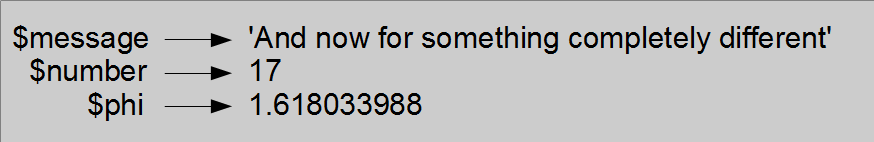
\includegraphics[scale=0.6]{figs/test_5.png}}
\caption{State diagram.}
\label{fig.state2}
\end{figure}



\section{Variable Names}
\index{variable}

Programmers generally choose names for their variables that
are meaningful---they document what the variable is used for.

Variable names can be as long as you like.  They can contain
both letters and numbers, but user-defined variable names 
can't begin with a number. Variable names are case-sensitive, 
i.e., {\tt \$message} is not the same variable as {\tt \$Message} 
or {\tt \$MESSAGE}. It is legal to use uppercase letters, but 
it is conventional to use only lower case for most variables 
names. Some people nonetheless like to use {\tt \$TitleCase} 
for their variables or even pure {\tt \$UPPERCASE} for 
some special variables.
\index{lower case}
\index{upper case}
\index{title case}
\index{case!lower}
\index{case!upper}
\index{case!title}


\index{Unicode}
\index{ASCII}
Unlike most other programming languages, Perl~6 does not require 
the letters and digits used in variable names to be plain ASCII. 
You can use all kinds of Unicode letters, i.e., 
letters from almost any language in the world, so that, for example,  
{\tt \$brücke}, {\tt \$payé} or {\tt \$niño} are 
valid variable names, which can be useful for non-English 
programmers (provided that these Unicode characters are 
handled correctly by your text editor and your 
screen configuration). Similarly, instead of using 
\verb"$phi" for the name of the golden ratio variable, 
we might have used the \emph{Greek small letter phi}, \verb'φ' 
(Unicode code point U+03C6), just as we could have used 
the \emph{Greek small letter pi}, $\pi$,  for the well-known 
circle circumference to diameter ratio:
\index{golden ratio}
\index{Unicode}
\index{phi}
\index{pi}

\begin{verbatim}
> my $φ = (5 ** .5 + 1)/2;       # golden ratio
1.61803398874989
> say 'Variable $φ = ', $φ;
Variable $φ = 1.61803398874989
> my $π = 4 * atan 1; 
3.14159265358979
> # you could also use the pi or π built-in constant:
> say pi
3.14159265358979
\end{verbatim}

The underscore character, \verb"_", can appear anywhere in a variable name.
It is often used in names with multiple words, such as 
\verb"$your_name" or \verb"$airspeed_of_unladen_swallow". 
\index{underscore character}

You may even use dashes to create so-called 
``kebab case''\footnote{Because the 
words appear to be skewered like pieces of food prepared for 
a barbecue.} and name those variables 
\verb"$your-name" or \verb"$airspeed-of-unladen-swallow", and this 
might make them slightly easier to read: a dash \verb'-' is 
valid in variable names provided it is immediately followed by an 
alphabetical character and preceded by an alphanumerical character. 
For example, \verb"$double-click" or \verb"$la-niña" are legitimate 
variable names. Similarly, you can use an apostrophe \verb"'" 
(a.k.a. single quote) between letters, so \verb"$isn't" or 
\verb"$o'brien's-age" are valid identifiers.
\index{dash}
\index{apostrophe}
\index{single quote}
\index{quote!single}
\index{kebab case}
\index{case!kebab}


If you give a variable an illegal name, you get a syntax error:
\index{syntax error}

\begin{verbatim}
> my $76trombones = 'big parade'
===SORRY!=== Error while compiling <unknown file>
Cannot declare a numeric variable
at <unknown file>:1
------> my $76<HERE>trombones = "big parade";
>
> my $more§ = 100000;
===SORRY!=== Error while compiling <unknown file>
Bogus postfix
at <unknown file>:1
------> my $more<HERE>§ = 100000;
(...)
\end{verbatim}
%
{\tt \$76trombones} is illegal because it begins with a number.
{\tt \$more§} is illegal because it contains an illegal character, {\tt
§}. 

If you've ever used another programming language and stumbled 
across a terse message such as {\tt"SyntaxError: invalid syntax"}, 
you will notice that the Perl designers have made quite a bit 
of effort to provide detailed, useful, and meaningful error 
messages. 
\index{error message}

Many programming languages have \emph{keywords} or \emph{reserved 
words} that are part of the syntax, such as {\tt if}, {\tt while}, 
or {\tt for}, and thus cannot be used for identifying variables 
because this would create ambiguity. There is no such problem 
in Perl: since variable names start with a sigil, the compiler 
is always able to tell the difference between a keyword and a 
variable. Names such as {\tt \$if} or {\tt \$while} are 
syntactically valid variable identifiers in Perl (whether 
such names make sense is a different matter).
\index{sigil}
\index{keyword}
\index{reserved word}



\section{Expressions and Statements}
\label{expr_and_statements}

An {\bf expression} is a combination of terms and operators.
Terms may be variables or literals, i.e., constant values such as a number or a string. A value all by itself is considered an expression, and so is
a variable, so the following are all legal expressions:
\index{expression}
\index{term}
\index{literal}

\begin{verbatim}
> 42
42
> my $n = 17;
17
> $n;
17
> $n + 25;
42
>
\end{verbatim}
%
When you type an expression at the prompt, the interpreter
{\bf evaluates} it, which means that it finds the value of
the expression.
In this example, {\tt \$n} has the value 17 and
{\tt \$n + 25} has the value 42.
\index{evaluate}

A {\bf statement} is a unit of code that has an effect, like
creating a variable or displaying a value, and usually needs to end 
with a semi-colon {\tt ;} (but the semi-colon can sometimes be omitted 
as we will see later):
\index{statement}
\index{semi-colon}

\begin{verbatim}
> my $n = 17;
17
> say $n;
17
\end{verbatim}
%

The first line is an assignment statement that gives a value to
{\tt \$n}.  The second line is a print statement that displays the
value of {\tt \$n}.

When you type a statement and then press {\tt Enter}, the 
interpreter {\bf executes} it, which means that it does 
whatever the statement says.
\index{execute}

An assignment can be combined with expressions using arithmetic 
operators. For example, you might write:
\index{operator}

\begin{verbatim}
> my $answer = 17 + 25;
42
> say $answer;
42
\end{verbatim}
%

The \verb'+' symbol is obviously the addition operator 
and, after the assignment statement, the \verb'$answer' 
variable contains the result 
of the addition. The terms on each side of the operator 
(here 17 and 25) are sometimes called the \emph{operands} 
of the operation (an addition in this case).
\index{operand}
\index{addition operator}
\index{assignment}

Note that the REPL actually displays the result of the 
assignment (the first line with ``42''), so that the 
print statement was not really necessary in this 
example \emph{under the REPL}; from now on, for the sake of 
brevity, we will generally omit the print statements in the 
examples where the REPL displays the result.
\index{REPL}

In some cases, you want to add something to a variable 
and assign the result to that same variable. This could 
be written:

\begin{verbatim}
> my $answer = 17;
17
> $answer = $answer + 25;
42
\end{verbatim}
%

Here, \verb"$answer" is first declared with a value of 17. The next 
statement assigns to \verb"$answer" the current value of 
\verb"$answer" (i.e., 17) + 25. This is such a common operation 
that Perl, like many other programming languages, has a 
shortcut for this:

\begin{verbatim}
> my $answer = 17;
17
> $answer += 25;
42
\end{verbatim}
%

\index{$+=$ augmented assignment operator}
The \verb"+=" operator combines the arithmetic addition operator 
and the assignment operator to modify a value and apply the result 
to a variable in one go, so that \verb"$n += 2" means: take 
the current value of \verb"$n", add 2, and assign the result to 
\verb"$n". This syntax works with all other arithmetic operators. 
For example, \verb"-=" similarly performs a subtraction and an 
assignment, \verb"*=" a multiplication and an assignment, etc. It 
can even be used with operators other than arithmetic operators, 
such as the string concatenation operator that we will see later.

Adding 1 to a variable is a very common version of this, so that 
there is a shortcut to the shortcut, the \emph{increment} operator, 
which increments its argument by one, and returns the incremented value:
\index{increment operator}
\index{++ increment operator}
\index{operator!++ (increment)}

\begin{verbatim}
> my $n = 17;
17
> ++$n;
18
> say $n;
18
\end{verbatim}
%
This is called the prefix increment operator, because the \verb"++" 
operator is placed before the variable to be incremented. There is 
also a postfix version, \verb"$n++", which first returns the current 
value and then increments the variable by one. It would not make 
a difference in the code snippet above, but the result can be very different 
in slightly more complex expressions. 

There is also a decrement operator \verb"--", which decrements its 
argument by one and also exists in a prefix and a postfix form. 
\index{decrement operator}
\index{\verb'--' decrement operator}
\index{operator!$--$ (decrement)}



\section{Script Mode}

So far we have run Perl in {\bf interactive mode}, which
means that you interact directly with the interpreter (the 
REPL). Interactive mode is a good way to get started,
but if you are working with more than a few lines of code, 
it can be clumsy and even tedious.
\index{interactive mode}

The alternative is to use a text editor and save code in a file 
called a {\bf script} and then run the interpreter in {\bf script mode} 
to execute the script.  By convention, Perl~6 scripts have names that 
end with {\tt .pl}, {\tt .p6} or {\tt .pl6}.
\index{script}
\index{script mode}

Please make sure that you're really using a \emph{text editor} 
and not a \emph{word-processing program} (such as MS Word, 
OpenOffice or LibreOffice Writer). There is a very large 
number of text editors available for free. On Linux, you might use 
\emph{vi} (or \emph{vim}), \emph{emacs}, \emph{gEdit}, or 
\emph{nano}. On Windows, you may use \emph{notepad} (very limited) 
or \emph{notepad++}. There are also many cross-platform editors  
or integrated development environments (IDEs) providing a 
text editor functionality, including \emph{padre}, \emph{eclipse}, 
or \emph{atom}. Many of these provide various syntax highlighting 
capabilities, which might help you use correct syntax (and 
find some syntax errors).
\index{syntax!highlighting}
\index{text editor!emacs}
\index{text editor!vi}
\index{text editor!vim}
\index{text editor!gEdit}
\index{text editor!padre}
\index{text editor!eclipse}
\index{text editor!nano}
\index{text editor!notepad++}
\index{text editor!atom}

Once you've saved your code into a file (say, for example, 
\verb'my_script.pl6'), you can run the program by issuing 
the following command at the operating system prompt (for example 
in a Linux console or in a \verb'cmd' window under Windows):
\begin{verbatim}
perl6 my_script.pl6
\end{verbatim}

Because Perl provides both modes,
you can test bits of code in interactive mode before you put them
in a script.  But there are differences between interactive mode
and script mode that can be confusing.
\index{interactive mode}
\index{script mode}

For example, if you are using the Perl~6 interpreter as a 
calculator, you might type:

\begin{verbatim}
> my $miles = 26.2;
26.2
> $miles * 1.61;
42.182
\end{verbatim}

The first line assigns a value to {\tt \$miles} and displays that value.  
The second line is an expression, so the
interpreter evaluates it and displays the result.  It turns out that a
marathon is about 42~kilometers.

But if you type the same code into a script and run it, you get no
output at all.  In script mode, an expression, all by itself, has no
visible effect.  Perl actually evaluates the expression, but it doesn't
display the value unless you tell it to:

\begin{verbatim}
my $miles = 26.2;
say $miles * 1.61;
\end{verbatim}

This behavior can be confusing at first. Let's examine why.

A script usually contains a sequence of statements.  If there
is more than one statement, the results appear one at a time
as the print statements execute.

For example, consider the following script:

\begin{verbatim}
say 1;
my $x = 2;
say $x;
\end{verbatim}
%
It produces the following output:

\begin{verbatim}
1
2
\end{verbatim}
%
The assignment statement produces no output.

To check your understanding, type the following statements in the
Perl interpreter and see what they do:

\begin{verbatim}
5;
my $x = 5;
$x + 1;
\end{verbatim}

Now put the same statements in a script and run it.  What
is the output?  Modify the script by transforming each
expression into a print statement and then run it again.

\section{One-Liner Mode}

Perl also has a \emph{one-liner mode}, which enables you 
to type directly a very short script at the operating 
system prompt. Under Windows, it might look like this:
\index{one-liner mode}
\label{one-liner mode}

\begin{verbatim}
C:\Users\Laurent>perl6 -e "my $value = 42; say 'The answer is ', $value;"
The answer is 42

\end{verbatim}

The {\tt -e} option tells the compiler that the script to 
be run is not saved in a file but instead typed at the 
prompt between quotation marks immediately after 
this option.

Under Unix and Linux, you would replace double quotation 
marks with apostrophes (or single quotes) 
and apostrophes with double quotation marks:
\index{apostrophe}
\index{quote mark}

\begin{verbatim}
$  perl6 -e 'my $value = 42; say "The answer is $value";'
The answer is 42

\end{verbatim}

The one-liner above may not seem to be very useful, but 
throwaway one-liners can be very practical to perform 
simple one-off operations, such as quickly modifying 
a file not properly formatted, without having to save a script 
in a separate file before running it.

We will not give any additional details about the one-liner 
mode here, but will give some more useful examples 
later in this book; for example, 
Subsection~\ref{one-liner-example},
Subsection~\ref{rot13_oneliner} (solving the ``rot-13'' exercise), or
Subsection~\ref{sol_cartalk} (solving the exercise on 
consecutive double letters). 



\section{Order of Operations}
\index{order of operations}
\index{PEMDAS}
\index{operator precedence}
\index{precedence!operator}

When an expression contains more than one operator, the order of
evaluation depends on the {\bf order of operations} or \emph{operator precedence}. 
For mathematical operators, Perl follows mathematical convention.
The acronym {\bf PEMDAS}\footnote{US students are sometimes taught 
to use the "Please Excuse My Dear Aunt Sally" mnemonics to remember 
the right order of the letters in the acronym.} is a useful 
way to remember the rules:

\begin{itemize}

\item {\bf P}arentheses have the highest (or tightest) precedence and can be used 
to force an expression to evaluate in the order you want. Since
expressions in parentheses are evaluated first, {\tt 2 * (3-1)} is 4,
and {\tt (1+1)**(5-2)} is 8. You can also use parentheses to make an
expression easier to read, as in {\tt (\$minute * 100) / 60}, even
if it doesn't change the result.
\index{$()$ parenthesis operator}

\item {\bf E}xponentiation has the next highest precedence, so
{\tt 1 + 2**3} is 9 (1 + 8), not 27, and {\tt 2 * 3**2} is 18, not 36.
\index{$**$ exponentiation operator}
\index{operator!$**$ (exponentiation)}

\item {\bf M}ultiplication and {\bf D}ivision have higher precedence
  than {\bf A}ddition and {\bf S}ubtraction.  So {\tt 2*3-1} is 5, not
  4, and {\tt 6+4/2} is 8, not 5.
\index{$*$ multiplication operator}
\index{operator!$*$ (multiplication)}
\index{$/$ division operator}
\index{operator!$/$ (division)}

\item Operators with the same precedence are usually evaluated 
from left to right (except exponentiation).  So in the expression 
{\tt \$degrees / 2 * pi}, the division happens first and the 
result is multiplied by {\tt pi}, which is not the expected 
result. (Note that {\tt pi} is not a variable, but a predefined 
constant in Perl~6, and therefore does not require a sigil.)  To 
divide by $2 \pi$, you can use parentheses:
\index{sigil}
\index{pi}
  
\begin{verbatim}
my $result = $degrees / (2 * pi);  
\end{verbatim}  
 
or write
  {\tt \$degrees / 2 / pi} or {\tt \$degrees / 2 / $\pi$}, which
  will divide \verb'$degrees' by 2, and then divide the result of 
  that operation by $\pi$ (which is equivalent to \verb'$degrees'
  divided by $2 \pi$).

\end{itemize}

I don't work very hard to remember the precedence of
operators.  If I can't tell by looking at the expression, I use
parentheses to make it obvious. If I don't know for sure which of two operators 
has the higher precedence, then the next person reading or maintaining 
my code may also not know.
\index{precedence}
\index{parentheses}


\section{String Operations}
\label{string_operations}
\index{string!operation}
\index{operator!string}
\index{coercion}
\index{type!coercion}

In general, you can't perform mathematical operations on strings, unless
the strings look so much like numbers that Perl can transform or \emph{coerce} them into numbers and still make sense, so the 
following are illegal:

\begin{verbatim}
'2'-'1a'    'eggs'/'easy'    'third'*'a charm'
\end{verbatim}
%

For example, this produces an error:

\begin{verbatim}
> '2'-'1a'
Cannot convert string to number: trailing characters after number 
in '1?a' (indicated by ?)
  in block <unit> at <unknown file>:1
\end{verbatim}
%
  
But the following expressions are valid because these strings 
can be coerced to numbers without any ambiguity:
\begin{verbatim}
> '2'-'1'
1
> '3'/'4'
0.75
\end{verbatim}
%

The \verb'~' operator performs {\bf string concatenation}, which means
it joins the strings by linking them end-to-end.  For example:
\index{string concatenation}
\index{string!concatenation}

\begin{verbatim}
> my $first = 'throat'
throat
> my $second = 'warbler'
warbler
> $first ~ $second
throatwarbler
\end{verbatim}
%
The {\tt x} operator also works on strings; it performs repetition.
For example:
\index{string repetition}

\begin{verbatim}
> 'ab' x 3;
ababab
> 42 x 3
424242
> 3 x 42
333333333333333333333333333333333333333333
\end{verbatim}

Notice that, although the {\tt x} operator somewhat looks like 
the multiplication operator when we write it by hand, {\tt x} 
is obviously not commutative, contrary to the {\tt *} 
multiplication operator. The first operand is a string or is 
\emph{coerced} to a string (i.e., transformed into a string: 
{\tt 42} is coerced to {\tt '42'}), and the second operand 
has to be a number or something that can be transformed 
into a number.
\index{commutativity}
\index{coercion}


\section{Comments}
\index{comment}

As programs get bigger and more complicated, they get more difficult
to read.  Formal languages are dense, and it is often difficult to
look at a piece of code and figure out what it is doing, or why.

For this reason, it is a good idea to add notes to your programs to explain
in natural language what the program is doing.  These notes are called
{\bf comments}, and they start with the \verb"#" symbol:

\begin{verbatim}
# compute the percentage of the hour that has elapsed
my $percentage = ($minute * 100) / 60;
\end{verbatim}
%
In this case, the comment appears on a line by itself.  You can also put
comments at the end of a line:

\begin{verbatim}
$percentage = ($minute * 100) / 60;     # percentage of an hour
\end{verbatim}
%
Everything from the {\tt \#} to the end of the line is ignored---it
has no effect on the execution of the program.

Comments are most useful when they document nonobvious features of
the code.  It is reasonable to assume that the reader can figure out
{\em what} the code does; it is more useful to explain {\em why}.

This comment is redundant with the code and useless:

\begin{verbatim}
my $value = 5;        # assign 5 to $value
\end{verbatim}
%
This comment, by contrast, contains useful information that 
is not in the code:

\begin{verbatim}
my $velocity = 5;     # velocity in meters/second. 
\end{verbatim}
%
Good variable names can reduce the need for comments, but
long names can make complex expressions hard to read, so there is
a tradeoff.
\index{variable name}


\section{Debugging}
\index{debugging}
\index{bug}

Three kinds of errors can occur in a program: syntax errors, runtime 
errors, and semantic errors.  It is useful
to distinguish between them in order to track them down more quickly.

\begin{description}

\item[Syntax error] ``Syntax'' refers to the structure of a program
  and the rules about that structure.  For example, parentheses have
  to come in matching pairs, so {\tt (1 + 2)} is legal, but 
{\tt 8)} is a \emph{syntax error}. \footnote{We are using 
``syntax error'' here as a quasi-synonym for ``compile-time error''; 
they are not exactly the same thing (you may in theory have 
syntax errors that are not compile-time errors and the other way 
around), but they can be deemed to be the same for 
practical purposes here. In Perl~6, compile-time errors 
have the ``===SORRY!==='' string at the beginning of 
the error message.}

\index{error!syntax}
\index{error message}
\index{syntax} 
\index{syntax!error}

If there is a syntax error
anywhere in your program, Perl displays an error message and quits 
without even starting to run your program, and you will 
obviously not be able to run the program.  During the first few
weeks of your programming career, you might spend a lot of
time tracking down syntax errors.  As you gain experience, you will
make fewer errors and find them faster.


\item[Runtime error] The second type of error is a runtime error, so
  called because the error does not appear until after the program has
  started running.  These errors are also called \emph{exceptions}
  because they usually indicate that something exceptional (and bad)
  has happened.  \index{runtime error} \index{error!runtime}
  \index{exception} \index{safe language} \index{language!safe}

Runtime errors are rare in the simple programs you will see in the
first few chapters, so it might be a while before you encounter one. 
We have seen one example of such errors, though, at the beginning 
of Section~\ref{string_operations} (p.~\pageref{string_operations}), 
when we tried to subtract \verb"'2'-'1a'". 


\item[Semantic error] The third type of error is \emph{semantic}, which
  means related to meaning.  If there is a semantic error in your
  program, it will run without generating error messages, but it will
  not do the right thing.  It will do something else.  Specifically,
  it will do what you \emph{told} it to do, but not what you 
  \emph{intended} it to do.
  \index{semantic error}
  \index{error!semantic} \index{error message}

Identifying semantic errors can be tricky because it requires you to work
backward by looking at the output of the program and trying to figure
out what it is doing.

\end{description}


\section{Glossary}

\begin{description}

\item[Variable]  Informally, a name that refers to a value. More 
accurately, a variable is a container that has a name and holds a value.
\index{variable}

\item[Assignment]  A statement that assigns a value to a variable.
\index{assignment}

\item[State diagram]  A graphical representation of a set of variables and the
values they refer to.
\index{state diagram}

\item[Keyword]  A reserved word that is used to parse a
program; in many languages, you cannot use keywords like 
{\tt if}, {\tt  for}, and {\tt while} as variable names. 
This problem usually does not occur in Perl because variable
names begin with a \emph{sigil}.
\index{keyword}
\index{sigil}

\item[Operand] A value or term next to an operator that 
is used in its evaluation.
\index{operand}

\item[Term]  A variable or a literal value.
\index{term}

\item[Expression]  A combination of operators and terms that
represents a single result.
\index{expression}

\item[Evaluate]  To simplify an expression by performing the operations
in order to yield a single value.
\index{evaluate}

\item[Statement]  A section of code that represents a command or action.  So
far, the statements we have seen are assignments and print statements. Statements usually end with a semi-colon.
\index{statement}

\item[Execute]  To run a statement and do what it says.
\index{execute}

\item[interactive mode (or interpreter mode):] A way of using the Perl 
interpreter by typing code at the prompt.
\index{interactive mode}

\item[Script mode] A way of using the Perl interpreter to read
code from a script and run it.
\index{script mode}

\item[one-liner mode:] A way of using the Perl interpreter to read
code passed at the operating system prompt and run it.
\index{one-liner mode}

\item[Script] A program stored in a file.
\index{script}

\item[Order of operations]  Rules governing the order in which
expressions involving multiple operators and operands are evaluated.
It is also called operator precedence.
\index{order of operations}
\index{operator precedence}
\index{precedence!operator}

\item[Concatenate]  To join two string operands end-to-end.
\index{concatenation}

\item[Comment]  Information in a program that is meant for other
programmers (or anyone reading the source code) and has no effect on the
execution of the program.
\index{comment}

\item[Syntax error]  An error in a program that makes it impossible
to parse (and therefore impossible to compile and to run).
\index{syntax!error}

\item[Exception]  An error that is detected while the program is running.
\index{exception}

\item[Semantics]  The meaning of a program.
\index{semantics}

\item[Semantic error]   An error in a program that makes it do something
other than what the programmer intended.
\index{semantic error}

\end{description}


\section{Exercises}

\begin{exercise}

Repeating our advice from the previous chapter, whenever you learn
a new feature, you should try it out in interactive mode (under 
the REPL) and make errors on purpose to see what goes wrong.
\index{interactive mode}
\index{REPL}

\begin{itemize}

\item We've seen that {\tt \$n = 42} is legal.  What about {\tt 42 = \$n}?

\item How about {\tt \$x = \$y = 1}? (Hint: note that you will 
have to declare both variables, for example with a statement 
such as {\tt my \$x; my \$y;} or possibly {\tt my (\$x, \$y);}, 
before you can run the above.)

\item In some languages, statements don't have to end with a semi-colon, 
{\tt ;}. What happens in script mode if you omit a semi-colon at the end
of a Perl statement?
\index{semi-colon}

\item What if you put a period at the end of a statement?

\item In math notation you can multiply $x$ and $y$ like this: $x y$.
What happens if you try that in Perl?

\end{itemize}

\end{exercise}


\begin{exercise}

Practice using the Perl interpreter as a calculator: 
\index{calculator}

\begin{enumerate}

\item The volume of a sphere with radius $r$ is $\frac{4}{3} \pi r^3$.
  What is the volume of a sphere with radius 5?

\item Suppose the cover price of a book is \$24.95, but bookstores get a
  40\% discount.  Shipping costs \$3 for the first copy and 75 cents
  for each additional copy.  What is the total wholesale cost for
  60 copies?

\item If I leave my house at 6:52 a.m. and run 1 mile at an easy pace
  (8:15 per mile), then 3 miles at tempo (7:12 per mile) and 1 mile at
  easy pace again, what time is it when I complete my running exercise?
\index{running pace}

\end{enumerate}
\end{exercise}



\chapter{Functions}
\label{funcchap}

In the context of programming, a {\bf function} 
is usually a named sequence of statements 
that performs a computation.  In Perl, functions are often 
also called {\bf subroutines} and the two terms can (for now) 
be considered as more or less equivalent. When you define 
a function, you specify the name and the sequence of statements.  
Later, when you want to perform a computation, you can ``call'' 
the function by name and this will run the sequence of statements 
contained in the function definition.
\index{function}

Perl comes with many built-in functions that are quite handy.  
You've already seen some of them: for example, {\tt say} is a 
built-in function, and we will see many more in the course of 
this book. And if Perl doesn't already have a function that does 
what you want, you can build your own. This teaches you the basics 
of functions and how to build new ones.

\section{Function Calls}
\label{functionchap}
\index{function!call}

We have already seen examples of {\bf function calls}:

\begin{verbatim}
> say 42;
42
\end{verbatim}
%
The name of the function is {\tt say}.  The expression following 
the function name is called the {\bf argument} of the function. 
The {\tt say} function causes the argument to be displayed 
on the screen. If you need to pass several values to a function, 
then just separate the arguments with commas:
\begin{verbatim}
> say "The answer to the ultimate question is ", 42;
The answer to the ultimate question is 42
\end{verbatim}
%

Many programming languages require the arguments of a function to 
be inserted between parentheses. This is not required (and 
usually not recommended) in Perl~6 for most built-in functions 
(except when needed for precedence), but if you do use 
parentheses, you should make sure to avoid inserting spaces 
between the function name and the opening parenthesis. 
For example, the {\tt round} function usually takes two 
arguments: the value to be rounded and the unit or scale. 
You may call it in any of the following ways:

\begin{verbatim}
> round 42.45, 1;
42
> round 42.45, .1;
42.5
> round(42.45, .1);      # But not: round (42.45, .1);
42.5
> round( 42.45, .1);     # Space is OK *after* the opening paren
42.5
\end{verbatim}
\index{parentheses!argument in}

Experienced Perl programmers usually prefer to omit the parentheses 
when they can. Doing so makes it possible to chain several functions 
with a visually cleaner syntax. Consider for example the differences 
between these two calls:

\begin{verbatim}
> say round 42.45, 1;
42
> say(round(42.45, 1));
42
\end{verbatim}

The second statement is explicitly saying what is going on, but 
the accumulation of parentheses actually makes things 
not very clear. By contrast, the first statement can be seen 
as a pipeline to be read from right to left: the last function 
on the right, {\tt round}, is taking two arguments, 
{\tt 42.45, 1}, and the value produced by {\tt round} is 
passed as an argument to {\tt say}.

It is common to say that a function ``takes'' one or 
several arguments and ``returns'' a result.  The result is 
also called the {\bf return value}.
\index{argument}
\index{return!value}

Perl provides functions that convert values from one type 
to another.  When called with only one argument, the 
{\tt round} function takes any value and converts it to an 
integer, if it can, or complains otherwise:
\index{conversion!type}
\index{type!conversion}
\index{round function}
\index{function!round}

\begin{verbatim}
> round 42.3;
42
> round "yes"
Cannot convert string to number: base-10 number must begin with valid 
digits or '.' in '<HERE>yes' (indicated by <HERE>)
  in block <unit> at <unknown file> line 1
\end{verbatim}

%
Note that, in Perl~6, many built-in functions can also 
use a \emph{method invocation} syntax with the so-called 
dot notation. The following statements display the same result:
\index{invocation!method}
\index{method invocation}
\begin{verbatim}
> round 42.7;    # Function call syntax
43
> 42.7.round;    # Method invocation syntax
43
\end{verbatim}
%
The {\tt round} function can round off rational and 
floating-point values to integers. There is an {\tt Int} 
method that can also convert noninteger numerical values 
into integers, but it doesn't round off; it chops off the 
fraction part:
\index{Int method}
\index{method!Int}

\begin{verbatim}
> round 42.7
43
> 42.7.Int
42
\end{verbatim}

We'll come back to methods in the next section.

The {\tt Rat} built-in function converts integers and 
strings to rational numbers (if possible):
\index{Rat function}
\index{function!Rat}

\begin{verbatim}
> say 4.Rat;
4
> say 4.Rat.WHAT;
(Rat)
> say Rat(4).WHAT;
(Rat)
> say Rat(4).nude;
(4 1)
> say Rat('3.14159');
3.14159
> say Rat('3.14159').nude
(314159 100000)
\end{verbatim}
%
(As you might remember from Section~\ref{values_and_types}, 
the \verb'nude' method displays the \emph{nu}merator and 
\emph{de}nominator of a rational number.)

Finally, {\tt Str} converts its argument to a string:
\index{Str function}
\index{function!Str}

\begin{verbatim}
> say 42.Str.WHAT
(Str)
> say Str(42).WHAT;
(Str)
\end{verbatim}

\index{coercion}
\index{type!coercion}
Note that these type conversion functions often don't need 
to be called explicitly, as Perl will in many cases try to do the 
right thing for you. For example, if you have a string 
that looks like an integer number, Perl will \emph{coerce} 
the string to an integer for you if you try to apply 
an arithmetic operation on it:

\begin{verbatim}
> say "21" * "2";
42
\end{verbatim}

Similarly, integers will be coerced to strings if you 
apply the string concatenation operator to them:

\begin{verbatim}
> say 4 ~ 2;
42
> say (4 ~ 2).WHAT;
(Str)
\end{verbatim}

The coercion can even happen twice within the same expression 
if needed:

\begin{verbatim}
> say (4 ~ 1) + 1;
42
> say ((4 ~ 1) + 1).WHAT;
(Int)
\end{verbatim}

\section{Functions and Methods}
\index{function}
\index{method}

A method is similar to a function---it takes arguments and
returns a value---but the calling syntax is different. With 
a function, you specify the name of the function followed 
by its arguments. A method, by contrast, uses the dot 
notation: you specify the name of the object on which 
the method is called, followed by a dot and the name of 
the method (and possibly additional arguments).

A method call is often called an {\bf invocation}
\index{invocation}. The deeper differences between functions and
methods will become apparent much later, when studying 
object-oriented programming (in Chapter~\ref{objects}).
\index{invocation!method}
\index{method invocation}

For the time being, we can consider that the difference is 
essentially a matter of a different calling syntax when using Perl's 
built-ins. Most of Perl built-ins accept both a function 
call syntax and a method invocation syntax. For example, 
the following statements are equivalent:

\begin{verbatim}
> say 42;              # function call syntax
42
> 42.say;              # method invocation syntax
42
\end{verbatim}
%

You can also chain built-in routines with both syntactic 
forms:

\begin{verbatim}
> 42.WHAT.say;         # method syntax
(Int)
> say WHAT 42;         # function syntax
(Int)
> say 42.WHAT;         # mixed syntax
(Int)
\end{verbatim}
%

It is up to you to decide whether you prefer one form or the 
other, but we will use both forms, if only to get you used to 
both of them.

\section{Math functions}
\index{math function}
\index{function!math}

Perl provides most of the familiar mathematical functions.

For some less common functions, you might need to use a 
specialized module such as \verb'Math::Matrix' or 
\verb'Math::Trig'.  A {\bf module} is a file that contains a
collection of related functions.
\index{module}

Before we can use the functions in a module, we have to import it with
a {\bf use statement}:

\begin{verbatim}
use Math::Trig;
\end{verbatim}
%
This statement will import a number of functions that you will then be able to use as if you had defined them in your main source file, for example \verb'deg2rad' to perform conversion of angular values from degrees to radians, or \verb'rad2deg' to perform the opposite conversion.

For most common mathematical functions, however, you don't need any \verb'math' module, as they are included in the core of the language:

\begin{verbatim}
> my $noise-power = 5.5;
5.5
> my $signal-power = 125.6;
125.6
> my $decibels = 10 * log10 $signal-power / $noise-power;
13.5862694990693
\end{verbatim}
%
\index{log10 function}
\index{function!log10}
This first example uses \verb"log10" (common logarithm) 
to compute a signal-to-noise ratio in decibels 
(assuming that \verb"signal-power" and
\verb"noise-power" are defined in the proper units).  Perl 
also provides a {\tt log} function which, when receiving 
one argument, computes logarithm base {\tt e} of the argument, 
and, when receiving two arguments, computes the logarithm 
of the first argument to the base of the second argument:

\begin{verbatim}
> say e;                 # e is predefined as Euler's constant
2.71828182845905
> my $val = e ** e;
15.1542622414793
> say log $val;          # natural logarithm
2.71828182845905
> say log $val, e;       # logarithm base e or natural logarithm
2.71828182845905
> say log 1024, 2;       # binary logarithm or logarithm base 2
10
\end{verbatim}
%
\index{log function}
\index{function!log}


Perl also provides most common trigonometric functions:

\begin{verbatim}
> my $radians = 0.7;
0.7
> my $height = sin $radians;
0.644217687237691
\end{verbatim}

\index{sin function}
\index{radian}
\index{trigonometric function}
\index{function!trigonometric}
This example finds the sine of \verb'$radians'.  The name of the
variable is a hint that {\tt sin} and the other trigonometric
functions ({\tt cos}, {\tt tan}, etc.)  take arguments 
in radians. To convert from degrees to radians, you may 
use the  \verb'deg2rad' function of the 
\verb'Math::Trig module', or simply divide by 180 
and multiply by $\pi$:

\begin{verbatim}
> my $degrees = 45;
45
> my $radians = $degrees / 180.0 * pi;    # pi, predefined constant
0.785398163397448
> say sin $radians;       # should be square root of 2 divided by 2
0.707106781186547
\end{verbatim}
%
The expression {\tt pi} is a predefined constant for an
approximation of $\pi$, accurate to about 14 digits.
\index{pi}

If you know
trigonometry, you can check the previous result by comparing it to
the square root of two divided by two:
\index{sqrt function}
\index{function!sqrt}

\begin{verbatim}
> say sqrt(2) / 2;
0.707106781186548
\end{verbatim}
%

\section{Composition}
\index{composition}

So far, we have looked at the elements of a program---variables,
expressions, and statements---in isolation, without talking about how to combine them.

One of the most useful features of programming languages is their
ability to take small building blocks and {\bf compose} them, i.e., 
to combine them in such a way that the result of one is the 
input of another one.  For example, the argument of a function 
can be any kind of expression, including arithmetic operators:

\begin{verbatim}
> my $degrees = 45;
45
> my $height = sin($degrees / 360.0 * 2 * pi);
0.707106781186547
\end{verbatim}
%
Here, we have used parentheses for the argument to the {\tt sin} 
function to clarify that all the arithmetic operations 
within the parentheses are completed before the {\tt sin} function 
is actually called, so that it will use the result of these operations 
as its argument. 

You can also compose function calls:

\begin{verbatim}
> my $x = 10;
10
>  $x = exp log($x+1)
11
\end{verbatim}
%
Almost anywhere you can put a value, you can put an arbitrary
expression, with one exception: the left side of an assignment
statement has to be a variable name, possibly along with its
declaration.  Almost any other expression on the left
side is a syntax error \footnote{We will see rare exceptions to this rule
later}:

\begin{verbatim}
> my $hours = 1;
1
> my $minutes = 0;
0
> $minutes = $hours * 60;        # right 
60
> $hours * 60 = $minutes;        # wrong !!
Cannot modify an immutable Int
  in block <unit> at <unknown file> line 1
\end{verbatim}
%
\index{syntax error}


\section{Adding New Functions (a.k.a. Subroutines)}

\index{subroutine}
So far, we have only been using the functions that come with Perl,
but it is also possible to add new functions. In Perl, user-
defined functions are often called subroutines, but you might choose 
either word for them. 

A {\bf function definition} starts with the {\tt sub} keyword (for
subroutine) and specifies the name of a new subroutine and
the sequence of statements that run when the function is called.
\index{function}
\index{function!definition}
\index{definition!function}
\index{sub}

Here is an example of a subroutine quoting Martin Luther King's 
famous "I Have a Dream" speech at the Lincoln Memorial in 
Washington (1963):

\begin{verbatim}
sub print-speech() {
    say "Let freedom ring from the prodigious hilltops of New Hampshire.";
    say "Let freedom ring from the mighty mountains of New York.";
}
\end{verbatim}
%
{\tt sub} is a keyword that indicates that this is a subroutine
definition.  The name of the function is \verb"print-speech".  The
rules for subroutine names are the same as for variable names: letters,
numbers, and underscores are legal, as well as a dash or an 
apostrophe between letters, but the first character
must be a letter or an underscore.  You shouldn't use a 
language keyword (such as {\tt if} or {\tt while}) as 
the name of a function (in some cases, it might actually work, 
but it would be very confusing, at least for the human reader).
\index{sub!keyword}
\index{keyword!sub}
\index{argument}

The empty parentheses after the name indicate that this function
doesn't take any arguments. They are optional in that case, but are 
required when parameters need to be defined for the subroutine.
\index{parentheses!empty}
\index{header}
\index{body}

\index{indentation}
The first line of the subroutine definition is sometimes called 
the {\bf header}; the rest is called the {\bf body}.  The body 
has to be a code block placed between curly braces and it can contain
any number of statements. Although there is no requirement to do 
so, it is good practice (and highly recommended) to indent body 
statements by a few leading spaces, since it makes it easier to 
figure out visually where the function body starts and ends.
\index{curly bracket}
\index{curly brace}
\index{bracket!curly}


Please note that you cannot use a method-invocation syntax 
for subroutines (such as \verb"print-speech") that you write: 
you must call them with a function call syntax.
\index{method!invocation}
\index{function!call}
\index{invocation!method}
\index{method invocation}

The strings in the print statements are enclosed in double
quotes.  In this specific case, single quotes could have been 
used instead to do the same thing, but there are many cases 
where they wouldn't do the same thing, so you'll have to 
choose one or the other depending on the circumstances.
\index{double quote}
\index{quote!double}
\index{single quote}
\index{quote!single}


Most people use double quotes in cases where a single 
quote (which is also an apostrophe) appears in the string:
\index{apostrophe}
\begin{verbatim}
say "And so we've come here today to dramatize a shameful condition.";
\end{verbatim}
%
Conversely, you might use single quotes when double quotes 
appear in the string:
\begin{verbatim}
say 'America has given the Negro people a bad check, 
     a check which has come back marked "insufficient funds."';
\end{verbatim}
%
There is, however, a more important difference between single quotes 
and double quotes: double quotes allow variable interpolation, and 
single quotes don't.  Variable interpolation means that if a 
variable name appears within the double-quoted string, this 
variable name will be replaced by the variable value; within a 
single-quoted string, the variable name will appear verbatim. 
For example:
%
\begin{verbatim}
my $var = 42;
say "His age is $var.";            # -> His age is 42.
say 'Her age is $var.';            # -> Her age is $var.
\end{verbatim}
\index{interpolation}
\index{variable!interpolation}
%
The reason is not that the lady's age should be kept secret. 
In the first string, \verb'$var' is simply replaced within the 
string by its value, 42, because the string is quoted with double 
quotes; in the second string, \verb'$var' isn't replaced by 
its value because single 
quotes are meant to provide a more verbatim type of quoting 
mechanism. There are other quoting constructs offering finer 
control over the way variables and special characters are 
displayed in the output, but simple and double quotes are the most 
useful ones.

The syntax for calling the new subroutine is the same as
for built-in functions:

\begin{verbatim}
> print-speech();
Let freedom ring from the prodigious hilltops of New Hampshire.
Let freedom ring from the mighty mountains of New York.
\end{verbatim}
%

However, you cannot use the method-invocation syntax with 
such subroutines. We will see much later in this book (see 
Chapter~\ref{objects}) how to create methods. For the time 
being, we'll stick to the function-call syntax.
\index{invocation!method}
\index{method invocation}

Once you have defined a subroutine, you can use it inside another
subroutine.  For example, to repeat the previous excerpts of
King's address ,  we could write a subroutine called \verb"repeat_speech":

\begin{verbatim}
sub repeat-speech() {
    print-speech();
    print-speech();
}
\end{verbatim}
%
And then call \verb"repeat-speech":

\begin{verbatim}
> repeat-speech();
Let freedom ring from the prodigious hilltops of New Hampshire.
Let freedom ring from the mighty mountains of New York.
Let freedom ring from the prodigious hilltops of New Hampshire.
Let freedom ring from the mighty mountains of New York.
\end{verbatim}
%
But that's not really how the speech goes.


\section{Definitions and Uses}
\index{function!definition}

Pulling together the code fragments from the previous section, the
whole program looks like this:

\begin{verbatim}
sub print-speech () {
    say "let freedom ring from the prodigious hilltops of New Hampshire.";
    say "Let freedom ring from the mighty mountains of New York.";
}
sub repeat-speech () {
    print-speech();
    print-speech();
}
repeat-speech();
\end{verbatim}
%
This program contains two subroutine definitions: \verb"print-speech" and
\verb"repeat-speech".  Function definitions get executed just like other
statements, but the effect is to create the function.  The statements
inside the function do not run until the function is called, and
the function definition generates no output.

You don't have to create a subroutine before you can run it, 
the function definition may come after its call:
\begin{verbatim}
repeat-speech;
sub repeat-speech() {
    print_speech;
    print_speech;
}
sub print-speech() {
    # ...
}
\end{verbatim}


\section{Flow of Execution}
\index{flow of execution}

To ensure, for example, that a variable is defined (i.e., populated) 
before its first use, you have to know the order statements run in, 
which is called the {\bf flow of execution}.

Execution always begins at the first statement of the program 
(well, really \emph{almost} always, but let's say always 
for the time being). Statements are run one at a time, 
in order from top to bottom.

Subroutine definitions do not alter the flow of execution of the
program, but remember that statements inside a function don't
run until the function is called.

A function call is like a detour in the flow of execution. Instead of
going to the next statement, the flow jumps to the body of
the function, runs the statements there, and then comes back
to pick up where it left off.

That sounds simple enough, until you remember that one function can
call another.  While in the middle of one function, the program might
have to run the statements in another function.  Then, while
running that new function, the program might have to run yet
another function!

Fortunately, Perl is good at keeping track of where it is, so each
time a function completes, the program picks up where it left off in
the code that called it.  When it gets to the end of the program,
it terminates.

In summary, when you read a program, you
don't always want to read from top to bottom.  Sometimes it makes
more sense if you follow the flow of execution.


\section{Parameters and Arguments}
\label{parameters}
\index{parameter}
\index{function!parameter}
\index{argument}
\index{function!argument}

Some of the functions we have seen require arguments.  For
example, when you call {\tt sin} you pass a number
as an argument.  Some functions take more than one argument:
for example the {\tt round} function seen at the beginning 
of this chapter took two, the number to be rounded and 
the scale (although the {\tt round} function may accept a single argument, in which case the scale is defaulted to 1).

Inside the subroutine, the arguments are assigned to
variables called {\bf parameters}.  Here is a definition for
a subroutine that takes a single argument:
\index{parentheses!parameters in}

\begin{verbatim}
sub print-twice($value) {
    say $value;
    say $value
}
\end{verbatim}
%
This subroutine assigns the argument to a parameter
named \verb"$value". Another common way to say it is 
that the subroutine binds the parameter defined in its 
header to the argument with which it was called. When the 
above subroutine is called, it prints the content of the 
parameter (whatever it is) twice.

This function works with any argument value that can be printed:

\begin{verbatim}
> print-twice("Let freedom ring")
Let freedom ring
Let freedom ring
> print-twice(42)
42
42
> print-twice(pi)
3.14159265358979
3.14159265358979
\end{verbatim}
%
The same rules of composition that apply to built-in functions also
apply to programmer-defined subroutines, so we can use any kind of expression
as an argument for \verb"print-twice":
\index{composition}
\index{programmer-defined function}
\index{function!programmer defined}

\begin{verbatim}
> print-twice('Let freedom ring! ' x 2)
Let freedom ring! Let freedom ring! 
Let freedom ring! Let freedom ring! 
> print-twice(cos pi)
-1
-1
\end{verbatim}
%
The argument is evaluated before the function is called, so
in the examples the expressions \verb"'Let freedom ring! ' x 2" 
and {\tt cos pi} are only evaluated once.
\index{argument}

You can also use a variable as an argument:

\begin{verbatim}
> my $declaration = 'When in the Course of human events, ...'
> print-twice($declaration)
When in the Course of human events, ...
When in the Course of human events, ...
\end{verbatim}
%
The name of the variable we pass as an argument (\verb"$declaration") 
has nothing to do with the name of the parameter (\verb"$value"). It
doesn't matter what the variable was called back home (in the caller);
here, within \verb"print-twice", we call the parameter \verb"$value", 
irrespective of the name or content of the argument passed to the 
subroutine.


\section{Variables and Parameters Are Local}
\index{local variable}
\index{variable!local}
\index{scope}
\index{my}
\index{lexical scope}
\label{localvar}

When you create a variable inside a subroutine with the 
{\tt my} keyword, it is {\bf local}, or, more accurately, 
\emph{lexically scoped}, to the function block, which means 
that it only exists inside the function.  For example:
\index{parentheses!parameters in}

\begin{verbatim}
sub concat_twice($part1, $part2) {
    my $concatenation = $part1 ~ $part2;
    print-twice($concatenation)
}
\end{verbatim}
%
This function takes two arguments, concatenates them, and prints
the result twice.  Here is an example that uses it:
\index{concatenation}

\begin{verbatim}
> my $start = 'Let freedom ring from ';
> my $end = 'the mighty mountains of New York.';
> concat_twice($start, $end);
Let freedom ring from the mighty mountains of New York.
Let freedom ring from the mighty mountains of New York.
\end{verbatim}
%
When \verb"concat_twice" terminates, the variable \verb"$concatenation" 
is destroyed.  If we try to print it, we get an exception:
\index{Variable ... is not declared}
\index{exception!not declared}

\begin{verbatim}
> say $concatenation;
===SORRY!=== Error while compiling <unknown file>
Variable '$concatenation' is not declared
at <unknown file>:1
------> say <HERE>$concatenation;
\end{verbatim}
%
Parameters are also scoped to the subroutine.
For example, outside \verb"print-twice", there is no
such thing as \verb"$value".
\index{parameter}
\index{scope}


\section{Stack Diagrams}
\label{stackdiagram}
\index{stack diagram}
\index{function!frame}
\index{frame}

To keep track of which variables can be used where, it is sometimes
useful to draw a {\bf stack diagram}.  Like state diagrams, stack
diagrams show the value of each variable, but they also show the
function each variable belongs to.
\index{stack diagram}
\index{diagram!stack}

Each function is represented graphically by a {\bf frame}.  A frame 
is a box with the name of a function beside it and the parameters 
and variables of the function inside it.  The stack diagram for 
the previous example is shown in Figure~\ref{fig.stack}.

\begin{figure}
\centerline
{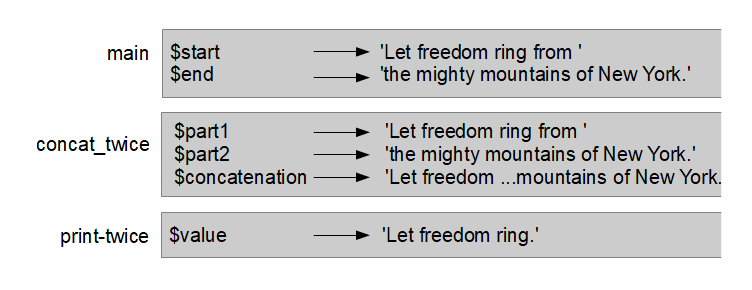
\includegraphics[scale=1.2]{figs/stack_diagram.png}}
\caption{Stack diagram.}
\label{fig.stack}
\end{figure}


The frames are arranged in a stack that indicates which function
called which, and so on.  In this example, \verb"print-twice"
was called by \verb"cat_twice", and \verb"cat_twice" was called by 
\verb"main", which is a special name for the topmost frame.  When
you create a variable outside of any function, it belongs to 
\verb"main".

Each parameter refers to the same value as its corresponding
argument.  So, {\tt \$part1} has the same value as
{\tt start}, {\tt \$part2} has the same value as {\tt \$end},
and {\tt \$value} has the same value as {\tt \$cat}.


\section{Fruitful Functions and Void Functions}
\index{fruitful function}
\index{void function}
\index{function, fruitful}
\index{function, void} 

Some of the functions we have used, such as the 
math functions, return results and are useful only insofar 
we use that return value; for lack of a better name, we 
may call them {\bf fruitful functions}.  Other functions, 
like \verb"print-twice", perform an action but don't appear 
to return a value (it does in fact return a value, {\tt True}, 
but we don't care about it).  They are sometimes called empty or 
{\bf void functions} in some other programming languages.

In some programming languages, such as Pascal or Ada, there 
is a strong distinction between a \emph{function} (which 
returns a value) and a \emph{procedure} (which doesn't); 
they are even defined with different keywords. This 
distinction does not apply to Perl and to most modern 
programming languages.

In fact, from a pure syntactic standpoint, Perl functions 
always return a result. So the distinction between 
``fruitful'' and ``void'' functions does not really exist 
syntactically, but only semantically, i.e., from the 
standpoint of the meaning of the program: maybe we need to 
use the return value, or maybe we don't.

Another distinction commonly made is between functions and 
mutators: functions do not change the initial state of the 
arguments they were called on, and mutators do modify it. We 
will not use this distinction here, but it is useful to 
keep it in mind.

When you call a fruitful function, you almost always
want to do something with the result; for example, you might
assign it to a variable or use it as part of an expression:

\begin{verbatim}
my $height = sin $radians;
my $golden = (sqrt(5) + 1) / 2;
\end{verbatim}
%
When you call a function in interactive mode (under the 
REPL), Perl usually displays the result:

\begin{verbatim}
> sqrt 5;
2.23606797749979
\end{verbatim}
%
But in a script, if you call a fruitful function all by 
itself, the return value is lost forever! In some cases, the 
compiler will be able to warn you, but not always. For example, 
consider the following program:

\begin{verbatim}
my $five = 5;
sqrt $five;
say $five;
\end{verbatim}

It produces the following warning:

\begin{verbatim}
WARNINGS for /home/Laurent/perl6_tests/sqrt.pl6:
Useless use of "sqrt $five" in expression "sqrt $five" in sink context (line 2)
5
\end{verbatim}
%
This script computes the square root of 5, but since 
it doesn't store or display the result, it is not very useful.
\index{interactive mode}
\index{script mode}

Void functions might display something on the screen, 
save some data to a file, modify a variable or an object, 
or have some other effect, but they generally don't have 
a return value, or at least not a useful one.  If you assign 
the result to a variable, you may get the return value of 
the subroutine, the value of the last expression which was 
evaluated in the function, or a special value such as 
{\tt Any}, which essentially means something that has not 
been defined, or {\tt Nil}.
\index{Any special value}
\index{special value!Any}
%

The subroutines we have written so far were essentially 
printing things to the screen. In that case, they 
usually return {\tt True}, at least when the printing 
was successful. Although they return a true value, what they 
return isn't very useful and we can consider them all void 
for our practical purposes.  

The following is an example of a very simple fruitful subroutine:
\index{return}

\begin{verbatim}
> sub square($number) { return $number ** 2 }
sub square ($number) { #`(Sub|118134416) ... }
> say square 5;
25
\end{verbatim}

The \verb'Sub|118134416' message displayed by the REPL is 
just an internal identifier for the subroutine we've just 
defined.

The {\tt return} statement instructs the function to terminate 
the execution of the function at this statement and to return 
the value of the following expression to the caller. In such a simple 
case where the program is in fact running the last statement 
of a function, the return keyword can be omitted since the function 
will return the value of the last evaluated statement, so that the 
{\tt square} subroutine could be written this way:
\begin{verbatim}
sub square($number) { 
    $number ** 2 
}
\end{verbatim}

We will be using fruitful functions more intensively in a 
few chapters.

\section{Function Signatures}
\index{function!signature}
\index{signature}

When a function receives arguments, which are stored into 
parameters, the part of the function 
definition describing the parameters between parentheses 
is called the {\bf function signature}. The function signatures 
we have seen so far are very simple and consist only of one 
parameter or possibly a parameter list.

Signatures can provide a lot more information about the 
parameters used by a function. First, you may define the 
type of the parameters. Some functions make sense only if their 
parameters are numeric and should probably raise an error if 
they get a string that cannot be converted to a numeric value. 
For example, if you define a function {\tt half} that computes 
a value equal to its argument divided by 2, it does not make 
sense to try to compute half of a string that is not numeric. 
It could be written as follows:
\index{type!parameter}
\index{parameter type}

\begin{verbatim}
sub half(Int $number) { 
    return $number / 2 
}
say half 84; # -> 42
\end{verbatim}

If this function is called with a string, we get the 
following error:
\index{type!String}

\begin{verbatim}
> say half "Douglas Adams"
===SORRY!=== Error while compiling <unknown file>
Calling half(Str) will never work with declared signature (Int $number)
at <unknown file>:1
------> say <HERE>half "Douglas Adams"
\end{verbatim}

The {\tt Int} type included in the function signature is a type 
constraint that can help prevent subtle bugs. In some cases, 
it can also be an annoyance. Consider this code snippet:
\index{constraint!type}
\index{type!constraint}
\index{type!Int}
\index{signature}


\begin{verbatim}
sub half(Int $number) {  $number / 2 }
say half "84"; # -> ERROR
\end{verbatim}

Because the argument to the {\tt half} subroutine is {\tt "84"}, 
i.e., a string, this code will fail with a type error. If we had 
not included the {\tt Int} type in the signature, the script 
would have converted (or \emph{coerced}) the "84" string to 
a number, divided it by two, and printed out the expected result:
\index{type!String}
\index{type!coercion}
\index{coercion!type}

\begin{verbatim}
sub half( $number) { $number / 2 }
say half "84"; # -> 42
\end{verbatim}

In some cases, you want this conversion to occur, in others 
you don't. It is up to you to decide whether you want 
strict typing or not, depending on the specific situation and
needs. It is probably helpful to use parameter typing in many 
cases, but it can also become a straitjacket in some situations. 
Perl~6 lets you decide how strict you want to be about these things.

Our original {\tt half} subroutine has another limitation: it
can work only on integers. But a function halving its argument 
should presumably be useful for rational or even other numbers. 
You can use the {\tt Real} or {\tt Numeric} types to make 
the function more general (the difference between the two 
types is that the {\tt Numeric} type will accept not only 
{\tt Real} but also {\tt Complex} numbers\footnote{~Complex 
numbers are a powerful concept of mathematics. They are numbers 
of the form $a + bi$, where $a$ and $b$ are usual real number and 
$i$ an imaginary number such that $i^2$ equals $-1$.}). As it turns out 
that this {\tt half} function will also work correctly 
with complex numbers, choosing a {\tt Numeric} 
type opens more possibilities:
\index{Numeric type}
\index{type!Numeric}
\index{Real type}
\index{type!Real}
\index{Complex type}
\index{type!Complex}
\index{type!Int}

\begin{verbatim}
sub half(Numeric $number) { $number / 2 }
say half(3+4i); # -> 1.5+2i
\end{verbatim}

The following table sums up and illustrates some of the 
various types we have seen so far.

\begin{center}
\begin{tabular}{|l|c|}  \hline
\label{types}
\emph{Type} & \emph{Example}   \\ \hline
String      & \verb'"A string"', \verb"'Another string'", \verb'"42"' \\ \hline
Integer     & \verb' -3, -2, 0, 2, 42' \\ \hline
Rational    & \verb' 1/2, 0.5, 3,14159, 22/7, 42.0' \\ \hline
Real        & $\pi$, pi, $\surd{2}$, \emph{e}, $\log 42$, $\sin 0.7$\\ \hline
Complex     & $5.4 + 3i$ \\ \hline
\end{tabular}
\end{center}
\index{String type}
\index{type!String}


\section{Immutable and Mutable Parameters}

\index{immutable parameter}
\index{mutable parameter}
\index{parameter!mutable}
\index{parameter!immutable}
By default, subroutine parameters are {\bf immutable} aliases for 
the arguments passed to the subroutine. In other words, they 
cannot be changed within the function and you cannot 
accidentally modify the argument in the caller:

\begin{verbatim}
sub plus-three(Int $number) { $number += 3}
my $value = 5;
say plus-three $value; # ERROR: Cannot assign to an immutable value
\end{verbatim}

In some other languages, this behavior is named a ``call 
by value'' semantic: loosely speaking, the subroutine 
receives (by default) a value rather than a variable, and 
the parameter therefore cannot be modified.
\index{call by reference}

If you want to change the value of the parameter within the 
subroutine (but without changing the argument in the caller) 
you can add the {\tt is copy} \emph{trait} to the signature:
\index{signature}
\index{trait}
\index{is copy trait}
\index{trait!is copy}

\begin{verbatim}
sub plus-three(Int $number is copy) { $number += 3}
my $value = 5;
say plus-three $value;  # 8
say $value;             # 5 (unchanged)
\end{verbatim}
%
A {\bf trait} is a property of the parameter defined at compile time. 
Here, the {\tt \$number} parameter is modified within the 
subroutine and the incremented value is returned to the caller 
and printed as 8, but, within the caller, the variable used
as an argument to the function, {\tt \$value}, is not 
modified (it is still 5).

Although this can sometimes be dangerous, you may also want 
to write a subroutine that modifies its argument at the caller 
side. For this, you can use the {\tt is rw} \emph{trait} 
in the signature:
\index{is rw trait}
\index{trait!is rw}

\begin{verbatim}
sub plus-three(Int $number is rw) { $number += 3}
my $value = 5;
say plus-three $value;  # 8
say $value;             # 8 ($value modified)
\end{verbatim}
%
With the {\tt is rw} trait, the {\tt \$number} parameter is 
now  \emph{bound} to the {\tt \$value} argument, so that any change 
made using {\tt \$number} within the subroutine will immediately 
be applied to {\tt \$value} at the caller side, because {\tt \$number} 
and {\tt \$value} are just different names for the same thing (they 
both refer to the same memory location). The argument is now 
fully \emph{mutable}.

In some other languages, this is named a ``call by reference'' 
parameter passing mechanism, because, in those languages, if you 
pass to a function  a reference (or a pointer) to a variable, then 
it is possible for the function to modify the variable referred 
to by the reference.
\index{call by reference}


\section{Functions and Subroutines as First-Class Citizens}
\index{first-class object}
\index{object, first-class}
\index{function!higher-order}
\label{first_class}

Subroutines and other code objects can be passed around as values, 
just like any variable, literal, or object. Functions are said 
to be {\bf first-class objects} or sometimes first-class 
citizens or higher-order functions. This means that a Perl 
function (its code, not the value returned by it) is a value 
you can assign to a variable or pass around as an argument. 
For example, \verb"do-twice" is a subroutine that takes a 
function as an argument and calls it twice:

\begin{verbatim}
sub do-twice($code) {
    $code(); 
    $code();
}
\end{verbatim}

Here, the \verb"$code" parameter refers to a function or some
other callable code object. This is an example that uses
\verb"do-twice" to call a function named \verb"greet" twice:

\begin{verbatim}
sub greet {
    say "Hello World!";
}
do-twice &greet;
\end{verbatim}

This will print:
\begin{verbatim}
Hello World!
Hello World!
\end{verbatim}

The \verb"&" sigil placed before the subroutine name in the 
argument list tells Perl that you are passing around a 
subroutine or some other callable code object (and not 
calling the subroutine at the moment).
\index{sigil}
\index{ampersand sigil}
%\index{$&$ sigil}
%\index{sigil!$&$}

In fact, it would be more idiomatic to also use the \verb"&" 
sigil in the \verb"do-twice" subroutine definition, to better 
specify that the parameter is a callable code object:
\index{idiomatic}

\begin{verbatim}
sub do-twice(&code) {
    &code(); 
    &code();
}
\end{verbatim}

or even:
\begin{verbatim}
sub do-twice(&code) {
    code(); 
    code();
}
\end{verbatim}

The syntax with the \verb"&" sigil has the benefit that 
it will provide a better error message if you make a mistake 
and pass something noncallable to \verb"do-twice". 

All the functions we have seen so far had a name, but a 
function does not need to have a name and can be \emph{anonymous}. 
For example, it may be stored directly in a scalar variable:
\index{anonymous function}
\index{function!anonymous}

\begin{verbatim}
my $greet = sub {
    say "Hello World!";
};
$greet();               # prints "Hello World"
do-twice $greet;        # prints "Hello World" twice
\end{verbatim}

It could be argued that the above \verb"$greet" subroutine  
is not really anonymous, since it is stored into a scalar 
variable that could in a certain way be considered as its name. 
But the subroutine really has no name; it just happens to be 
assigned to a scalar variable. Just to show that the subroutine 
can really have no name at all, consider this:

\begin{verbatim}
do-twice(sub {say "Hello World!"} );
\end{verbatim}

It will happily print "Hello World" twice. If the \verb"$do-twice"
function was declared earlier, you can even simplify the syntax 
and omit the parentheses:

\begin{verbatim}
do-twice sub {say "Hello World!"};
\end{verbatim}

For such a simple case where there is no need to pass an 
argument or return a value, you can even omit the 
\verb"sub" keyword and pass a code block directly to the function:
\index{code block}

\begin{verbatim}
do-twice {say "Hello World!"};
do-twice {say "what's up doc"};
\end{verbatim}

As you can see, \verb"do-twice" is a \emph{generic} subroutine in 
charge of just performing twice any function or code 
block passed to it, without any knowledge about what 
this function or code block is doing. This is a powerful 
concept for some relatively advanced programming techniques 
that we will cover later in this book.
\index{generic subroutine}

Subroutines may also be passed as return values from other 
subroutines:
\index{factory, function}
\index{function!factory}

\begin{verbatim}
> sub create-func ($person) { return sub { say "Hello $person!"}}
# Creating two greeting functions
sub create-func ($person) { #`(Sub|176738440) ... }
> my $greet_world = create-func "World";
sub () { #`(Sub|176738592) ... }
> my $greet_friend = create-func "dear friend";
sub () { #`(Sub|176739048) ... }
# Using the greet functions
> $greet_world();
Hello World!
> $greet_friend();
Hello dear friend!
\end{verbatim} 

Here, \verb"create-func" returns a subroutine greeting someone. 
It is called twice with two different arguments in order to 
create two different functions at runtime, \verb"$greet_world" and 
\verb"$greet_friend". A function such as \verb"create-func" 
is sometimes a \emph{function factory} because you may create as many 
functions as you like by just calling \verb"create-func". This 
example may seem to be a slightly complicated way of doing 
something quite simple. At this point, it is 
just a bit too early to give really useful examples, but 
this is also a very powerful programming technique.  

We'll come back to these techniques in various places in this 
book and even devote an entire chapter (chapter~\ref{functional 
programming}) to this subject and related topics.


\section{Why Functions and Subroutines?}
\index{function, reasons for}

It may not be clear why it is worth the trouble to divide
a program into functions or subroutines.  There are 
several reasons:

\begin{itemize}

\item Creating a new subroutine gives you an opportunity to 
name a group of statements, which makes your program easier 
to read and debug. Subroutines also help making the flow of 
execution clearer to the reader.

\item Subroutines can make a program smaller by eliminating 
repetitive code.  Later, if you make a change, you only have
to make it in one place.
\index{code repetition}

\item Dividing a long program into subroutines allows you 
to debug the parts one at a time and then assemble them 
into a working whole.

\item Well-designed subroutines are often useful for many programs.
Once you write and debug one, you can reuse it.
\index{code reuse}

\index{abstraction}
\item Creating subroutines is one of the major ways to 
break up a difficult problem into smaller easier subtasks 
and to create successive layers of abstraction, which are 
the key to solve complex problems.
\index{abstraction}

\index{black box}
\item Writing good subroutines lets you create black boxes, with 
a known input and a known output. So you don't have to think 
about them anymore when you're working on something else.  
They've become a tool.  Once you've assembled an electric 
screwdriver, you don't need to think about how it works internally 
when you use it to build or repair something.
\index{black box}

\item In the current open source world, chances are that your 
code will have to be understood, maintained, or enhanced by 
people other than you. Coding has become much more of a social 
activity than before. Breaking up your code into small subroutines 
whose purpose is easy to understand will make their work easier. 
And you'll be even more delighted when the person 
having to maintain or refactor your code is... you.
\index{open source code}

\end{itemize}


\section{Debugging}

One of the most important programming skills you will 
acquire is debugging. Although it can sometimes be 
frustrating, debugging is one of the most intellectually 
rich, challenging, and interesting parts of programming.
\index{experimental debugging}
\index{debugging!experimental}

In some ways debugging is like detective work.  You are confronted
with clues and you have to infer the processes and events that led
to the results you see.

Debugging is also like an experimental science.  Once you have an idea
about what is going wrong, you modify your program and try again.  If
your hypothesis was correct, you can predict the result of the
modification, and you take a step closer to a working program.  If
your hypothesis was wrong, you have to come up with a new one.  As
Sherlock Holmes pointed out, ``When you have eliminated the
impossible, whatever remains, however improbable, must be the truth''
(A. Conan Doyle, {\em The Sign of Four}).
\index{Holmes, Sherlock}
\index{Conan Doyle, Arthur}

In cases where you are not able to come up with a hypothesis 
on what's wrong, you can try to introduce code that you expect 
to create a certain type of error, a ``negative hypothesis'' 
if you will.  Sometimes you can learn a lot from the fact that 
it didn't create the error that was expected. Making a hypothesis 
does not necessarily mean you have an idea about how to make it 
work, it could also be a hypothesis on how it should break.

For some people, programming and debugging are the same thing.  That
is, programming is the process of gradually debugging a program until
it does what you want.  The idea is that you should start with a
working program and make small modifications,
debugging them as you go.

For example, Linux is an operating system that contains millions of
lines of code, but it started out as a simple program Linus Torvalds
used to explore the Intel 80386 chip.  According to Larry Greenfield,
``One of Linus's earlier projects was a program that would switch
between printing \verb"AAAA" and \verb"BBBB".  This later evolved 
to Linux.'' ({\em The Linux Users' Guide} Beta Version 1).
\index{Linux}


\section{Glossary}

\begin{description}

\item[Function] A named sequence of statements that performs 
some useful operation. Functions may or may not take arguments 
and may or may not produce a result. Perl comes with many 
built-in functions, and you can also create your own. In Perl, 
user-defined functions are often called subroutines.
\index{function}

\item[Function definition]  A statement that creates a new function,
specifying its name, parameters, and the statements it contains.
\index{function!definition}

\item[Header] The first line of a function definition.
\index{header}

\item[Body] The sequence of statements inside a function 
definition, usually in a code block delimited by braces.
\index{body}

\item[Parameter] A name used inside a subroutine to refer to 
the value passed as an argument.
\index{parameter}

\item[Function call] A statement that runs a function. It
consists of the function name followed by an argument list, 
which may or may not be enclosed within parentheses.
\index{function!call}

\item[Argument]  A value provided to a function when the function is called.
This value is assigned to the corresponding parameter in the function.
\index{argument}

\item[Lexical variable]  A variable defined inside a subroutine 
or a code block.  A lexical variable defined within a function can 
only be used inside that function.
\index{local variable}

\item[Return value]  The result of a function.  If a function call
is used as an expression, the return value is the value of
the expression.
\index{return!value}

\item[Any]  A special value typically found in variables that 
haven't been assigned a value. It is also a special value 
returned by some functions that we have called ``void'' (because 
they return something generally useless such as ``Any'').
\index{Any special value}
\index{special value!Any}

\item[Nil] Also a special value sometimes returned by some 
``void'' subroutines.

\item[Module] A file that contains a
collection of related functions and other definitions.
\index{module}

\item[Use statement] A statement that reads a module file and usually imports some functions.
\index{use statement}
\index{statement!use}

\item[Composition] Using an expression as part of a larger expression,
or a statement as part of a larger statement.
\index{composition}

\item[Flow of execution]  The order in which statements run.
\index{flow of execution}

\item[Stack diagram]  A graphical representation of a stack of subroutines,
their variables, and the values they refer to.
\index{stack diagram}

\item[Frame]  A box in a stack diagram that represents a subroutine call.
It contains the local variables and parameters of the subroutine.
\index{function!frame}
\index{frame}

\item[Fruitful function] A function or subroutine that returns a useful value.
\index{fruitful function}

\item[Void function] A function or subroutine that does not 
return a useful value.
\index{void function}

\item[Function signature] The part of the definition of a 
function (usually between parentheses) that defines its 
parameters and possibly their types and other properties.
\index{function!signature}
\index{signature}

\item[Immutable parameter] A function or subroutine parameter 
that cannot be changed within the function body. By default, 
subroutine parameters are immutable.
\index{immutable parameter}

\item[Trait] A property of a function or subroutine parameter 
that is defined at compile time.
\index{trait}

\item[First class object] Perl's subroutines are said to be
higher order objects or first-class objects, because they can 
be passed around as other subroutines' arguments or return values, 
just as any other objects.
\index{first-class object}
\index{object, first-class}

\item[Anonymous function] A function that has no name.
\index{anonymous function}
\index{function!anonymous}

\item[Function factory] A function that produces other functions as return values.
\index{factory, function}
\index{function!factory}

\end{description}


\section{Exercises}

\begin{exercise}
\index{chars function}
\index{function!chars}
\label{right_justify}

Write a subroutine named \verb"right-justify" that takes a string
named {\tt \$input-string} as a parameter and prints the 
string with enough leading spaces so that the last letter 
of the string is in column 70 of the display.

\begin{verbatim}[fontshape=up]
> right-justify('Larry Wall')
                                                           Larry Wall
\end{verbatim}

Hint: use string concatenation and repetition.  Also,
Perl provides a built-in function called {\tt chars} that
returns the length of a string, so the value of 
\verb"chars 'Larry Wall'" or \verb"'Larry Wall'.chars" is 10.
Solution: \ref{sol_right_justify}.

\end{exercise}


\begin{exercise}
\index{first-class object}
\index{object!first-class}
\index{do-twice}
\label{do_it_twice}


We have seen that functions and other code objects can be 
passed around as values, just like any object. Functions are said 
to be \emph{first-class objects}. For example, \verb"do-twice" is a function
that takes a function as an argument and calls it twice:

\begin{verbatim}[fontshape=up]
sub do-twice($code) {
    $code(); 
    $code();
}
sub greet {
    say "Hello World!";
}
do-twice(&greet);
\end{verbatim}

\begin{enumerate}

\item Type this example into a script and test it.

\item Modify \verb"do-twice" so that it takes two arguments, a
function and a value, and calls the function twice,
passing the value as an argument.

\item Copy the definition of 
\verb"print-twice" from earlier in this chapter to your script.

\item Use the modified version of \verb"do-twice" to call
\verb"print-twice" twice, passing ``What's up doc'' as an argument.

\item Define a new function called 
\verb"do-four" that takes a function and a value
and calls the function four times, passing the value
as a parameter.  There should be only
two statements in the body of this function, not four.

\end{enumerate}

Solution: \ref{sol_do_it_twice}.

\end{exercise}



\begin{exercise}
\label{draw_a_grid}
\index{print-grid}

Note: This exercise should be
done using only the statements and other features we 
have learned so far.  

\begin{enumerate}

\item Write a subroutine that draws a grid like the following:
\index{grid}

\begin{verbatim}[fontshape=up]
+ - - - - + - - - - +
|         |         |
|         |         |
|         |         |
|         |         |
+ - - - - + - - - - +
|         |         |
|         |         |
|         |         |
|         |         |
+ - - - - + - - - - +
\end{verbatim}
%
Hint: to print more than one value on a line, you can print
a comma-separated sequence of values:

\begin{verbatim}[fontshape=up]
  say '+', '-';
\end{verbatim}
%
The {\tt say} function prints its arguments with a newline at the end (it advances to the next line). If you don't want to 
go to the next line, use the {\tt print} function instead:


\begin{verbatim}[fontshape=up]
  print '+', ' ';
  print '-';
\end{verbatim}
%
The output of these statements is ``+ -''.

A {\tt say} statement with an empty string argument ends 
the current line and goes to the next line.

\item Write a subroutine that draws a similar grid
with four rows and four columns.

\end{enumerate}

Solution: \ref{sol_draw_a_grid}
\index{print-grid}.

Credit: this exercise is based on an exercise in Oualline, {\em
    Practical C Programming, Third Edition}, O'Reilly Media, 1997.

\end{exercise}



\chapter{Loops, Conditionals, and Recursion}
\label{conditionals}

The main topic of this chapter is the {\tt if} statement, which
executes different code depending on the state of the program.
But first I want to introduce two new operators: integer 
division and modulo.


\section{Integer Division and Modulo}

The {\bf integer division} operator, \verb"div", divides
two numbers and rounds down to an integer.  For example, 
suppose the
run time of a movie is 105 minutes.  You might want to know how
long that is in hours.  In Raku, conventional division
returns a rational number (in many languages, it returns a 
floating-point number, which is another kind of internal 
representation for noninteger numbers):

\begin{verbatim}
> my $minutes = 105;
> $minutes / 60;
1.75
\end{verbatim}

But we don't normally write hours with decimal points.  Integer 
division returns the integer number of hours, dropping the
fraction part:
\index{operator!div}
\index{div operator}
\index{integer division}

\begin{verbatim}
> my $minutes = 105;
> my $hours = $minutes div 60;
1
\end{verbatim}

In arithmetic, integer division is sometimes called 
\emph{Euclidean division}, which computes a quotient and a 
remainder.
\index{Euclidean division}
\index{division remainder}

To get the remainder, you could subtract off one hour in minutes:

\begin{verbatim}
> my $remainder = $minutes - $hours * 60;
45
\end{verbatim}

\index{integer division}
\index{floating-point division}
\index{division!integer}
\index{division!floating-point}
\index{modulo operator}
\index{operator!modulo}


An alternative is to use the {\bf modulo operator}, \verb"%", which
divides two numbers and returns the remainder:
%\index{$%$ modulo operator}
%\index{operator!$%$ (modulo)}

\begin{verbatim}
> my $remainder = $minutes % 60;
45
\end{verbatim}
%
The modulo operator is very common in programming languages
and is more useful than it seems.  For example, you can 
check whether one number is divisible by another---if 
{\tt \$dividend \% \$divisor} is zero, then {\tt \$dividend} 
is divisible by {\tt \$divisor}. This is commonly used, for 
example, with a divisor equal to 2 in order to determine 
whether an integer is even or odd. We will see an example 
of that later in this chapter (see Section~\ref{alternative.execution}).
\index{divisibility}
\index{even number}
\index{odd number}
\index{integer!even}
\index{integer!odd}

To tell the truth, Raku also has a specific operator for 
divisibility, \verb"%%". The \verb'$dividend %% $divisor' 
expression returns a true value if
\verb'$dividend % $divisor' is equal to 0,  
that is if {\tt \$dividend} is divisible by {\tt \$divisor} (and false otherwise):
\index{divisibility!operator}
\begin{verbatim}
> 42 %% 2;
True
\end{verbatim}

Also, you can extract the rightmost digit
or digits from a number with the modulo operator.  For example, {\tt \$x \% 10} yields the
rightmost digit of {\tt \$x} (in base 10).  Similarly, {\tt \$x \% 100}
yields the last two digits:

\begin{verbatim}
> 642 % 100;
42
\end{verbatim}
%
\index{modulo operator}
\index{operator!modulo}



\section{Boolean Expressions}
\index{Boolean expression}
\index{expression!Boolean}
\index{logical operator}
\index{operator!logical}

A {\bf Boolean expression} is an expression that is either true
or false.  The following examples use the operator {\tt ==}, 
which compares two numeric operands and produces
{\tt True} if they are equal and {\tt False} otherwise:

\begin{verbatim}
> 5 == 5;
True
> 5 == 6;
False
\end{verbatim}
%
{\tt True} and {\tt False} are special
values that belong to the type {\tt Bool}; they are not strings:
\index{True!special value}
\index{False!special value}
\index{special value!True}
\index{special value!False}
\index{Bool type}
\index{type!Bool}

\begin{verbatim}
> say True.WHAT
(Bool)
> say False.WHAT
(Bool)
\end{verbatim}
%
\index{operator!$==$ (numeric equality)}
\index{$==$ numeric equality operator}
The {\tt ==} operator is one of the {\bf numeric relational operators} 
and checks whether the operands are equal; the others are:

\begin{verbatim}
      $x != $y            # $x is not numerically equal to $y
      $x > $y             # $x is  numerically greater than $y
      $x < $y             # $x is  numerically less than $y
      $x >= $y            # $x is  numerically greater than or equal to $y
      $x <= $y            # $x is  numerically less than or equal to $y
      $x === $y           # $x and $y are truly identical
\end{verbatim}
% TODO: get these entries working in plastex
\ifplastex \else
\index{"!= numeric inequality operator@\texttt{"!=} numeric inequality operator}
\index{< less than numeric operator@\texttt{<} less than numeric operator}
\index{> greater than numeric operator@\texttt{>} greater than numeric operator}
\index{>= greater than or equal operator@\texttt{>=} greater than or equal operator}
\index{<= less than or equal operator@\texttt{<=} less than or equal operator}
\index{=== value identity operator@\texttt{===} value identity operator}
\index{operator!"!= (numeric inequality)@\texttt{"!=} (numeric inequality)}
\index{operator!< (numerically less than)@\texttt{<} (numerically less than)}
\index{operator!> (numerically greater than)@\texttt{>} (numerically greater than)}
\index{operator!>= (greater than or equal)@\texttt{>=} (greater than or equal)}
\index{operator!<= (less than or equal)@\texttt{<=} (less than or equal)}
\index{operator!=== (value identity)@\texttt{===} (value identity)}
\fi
Although these operations are probably familiar to you, the Raku
symbols are different from the mathematical symbols.  A common error
is to use a single equals sign ({\tt =}) instead of a double equals sign
({\tt ==}).  Remember that {\tt =} is an assignment operator and
{\tt ==} is a relational operator.   There is no such thing as
{\tt =<}, and there exists a {\tt =>} operator, but it is not 
a relational operator, but something completely different (it 
is, as we'll see later, a pair constructor).
\index{relational operator}
\index{relational operator!numeric}
\index{numeric relational operator}
\index{equality operator}
\index{operator!equal}
\index{operator!relational}
\index{pair constructor}
\index{constructor!pair}
% TODO: get these entries working in plastex
\ifplastex \else
\index{=> pair constructor@\texttt{=>} pair constructor}
\index{operator!=> (pair constructor)@\texttt{=>} (pair constructor)}
\fi

The difference between {\tt ==} and {\tt ===} is that the 
former operator checks whether the values of the operands 
are equal and the latter checks whether the operands are 
truly identical. As an example, consider this:

\begin{verbatim}
say 42 ==  42;           # True
say 42 ==  42.0;         # True
say 42 ===  42;          # True
say 42 === 42.0;         # False
\end{verbatim}
%


These relational operators can only compare numeric values
(numbers or variables containing numbers) or values that 
can be coerced to numeric values, such as, for example, 
the string "42" which, if used with these operators 
(except {\tt ===}), will be coerced to the number 42.
\index{coercion}

For comparing strings (in a lexicographic or ``pseudo-
alphabetic'' type of comparison), you need to use 
the {\bf string relational operators}:

\begin{verbatim}
      $x eq $y            # $x is string-wise equal to $y
      $x ne $y            # $x is string-wise not equal to $y
      $x gt $y            # $x is greater than $y (alphabetically after)
      $x lt $y            # $x is less than $y (alphabetically before)
      $x ge $y            # $x is greater than or equal to $y
      $x le $y            # $x is less than or equal to $y
      $x eqv $y           # $x is truly equivalent to $y
\end{verbatim}
%  
\index{relational operator}
\index{relational operator!string}
\index{string!relational operator}
\index{operator!relational}
\index{eq, string equality operator}
\index{operator!eq (string equality)}
\index{ne, string inequality operator}
\index{operator!ne (string inequality)}
\index{operator!gt (alphabetically after)}
\index{operator!lt (alphabetically before)}



For example, you may compare (alphabetically) two former 
US presidents:
\begin{verbatim}
> 'FDR' eq 'JFK';
False
> 'FDR' lt 'JFK';    # alphabetical comparison
True
\end{verbatim}
%  

Unlike most other programming languages, Raku allows you to chain relational operators transitively, just as in mathematical notation:

\begin{verbatim}
say 4 < 7 < 12;      # True
say 4 < 7 < 5;       # False
\end{verbatim}
\index{chained relational operator}

It may be useful to point out that numeric relational operators 
and string relational operators don't work the same way (and 
that's a good reason for having different operators), because 
they don't have the same idea of what is \emph{greater than} 
or \emph{less than}.

When comparing two positive integers, a number with four digits
is always greater than a number with only two or three digits. 
For example, 1110 is greater than 886. 

String comparisons, in contrast, basically follow (pseudo) 
alphabetical rules: ``b'' is greater than ``aaa'', because 
the commonly accepted rule for string comparisons is to start 
by comparing the first letter of each string: which string 
is greater is known if the two letters are different, 
irrespective of what character comes next; you need to proceed 
to comparing the second letter of each word only if comparing 
the first letter of each string led to a draw, and so on. 
Thus, any word starting with ``a'' is less than any word 
starting with ``b'', irrespective of the length of these 
words. You may think that this is nitpicking, but this 
becomes essential when you start sorting items: you really 
have to think about which type of order (numeric or 
alphabetical) you want to use.
\index{sorting}

There are also some so-called ``three-way'' relational operators, 
{\tt cmp}, {\tt <=>} and {\tt leg}, but we'll come back to them 
when we study how to sort the items of a list. Similarly, we need 
to learn quite a few other things about Raku before we can do 
justice to the incredibly powerful and expressive \emph{smart match} 
operator, \verb"~~".
\index{sorting}
\index{smart match operator}
\index{operator!smart match}
\index{three-way operator}
\index{operator!three-way}
\index{cmp operator}
\index{leg operator}
\index{operator!leg}
% TODO: get these entries working in plastex
\ifplastex \else
\index{<=> operator@\texttt{<=>} operator}
\index{operator!<=> (numeric comparison)@\texttt{<=>} (numeric comparison)}
\fi

A final point to be noted about string comparisons is 
that uppercase letters are always deemed smaller 
than lowercase letters. So "A," "B," "BB," and "C" 
are \emph{all} less than "a," "b," "bb," and "c." We 
will not go into the details here, but this becomes 
more complicated (and sometimes confusing) when 
the strings to be compared contain nonalphabetical 
characters (or non-ASCII Unicode letters).

\section{Logical Operators}
\index{logical operator}
\index{operator!logical}

There are three main pairs of {\bf logical operators}: 
\begin{itemize}
\item logical \emph{and}: ``{\tt and}'' and {\tt \&\&}
\item logical \emph{or}: ``{\tt or}'' and {\tt ||}
\item logical \emph{not}: ``{\tt not}'' and {\tt !}
\end{itemize}

The semantics (meaning) of these operators is
similar to their meaning in English.  For example,
{\tt \$x > 0 and \$x < 10} is true only if {\tt \$x} is greater 
than 0 {\em and} less than 10.
\index{and operator}
\index{or operator}
\index{not operator}
\index{operator!and}
\index{operator!or}
\index{operator!not}

{\tt \$n \% 2 == 0 and \$n \% 3 == 0} is true if {\em both} 
conditions are true, that is, if the number is divisible by 2
{\em and} by 3, i.e., is in fact divisible by 6 (which could be better 
written as: {\tt \$n \% 6 == 0} or {\tt \$n \%\% 6}).

{\tt \$n \% 2 == 0 or \$n \% 3 == 0} is true if {\em either or 
both} of the conditions is true, that is, if the number is 
divisible by 2 {\em or} by 3 (or both).

Finally, the {\tt not} operator negates a Boolean
expression, so {\tt not (x > y)} is true if {\tt x > y} 
is false, that is, if {\tt x} is less than or equal 
to {\tt y}.

The {\tt \&\&}, {\tt ||}, and {\tt !} operators have the same 
meanings, respectively, as {\tt and}, {\tt or}, and {\tt not}, 
but they have a tighter precedence, which means that when 
they stand in an expression with some other operators, 
they have a higher priority of execution. We will come 
back to precedence later, but let's say for the time being 
that, in most common cases, the {\tt and}, {\tt or}, and 
{\tt not} operators will usually do what you want.
\index{precedence}      
\index{operator precedence}

Strictly speaking, the operands of the logical operators should 
be Boolean expressions, but Raku, just like many languages 
partly derived from C, is not very strict on that. The 
numbers~0 and 0.0 are false; and any nonzero number 
or nonempty string is interpreted as {\tt True}:

\begin{verbatim}
> 42 and True;
True
\end{verbatim}
%
This flexibility can be very useful, but there are some 
subtleties to it that might be confusing.  You might want 
to avoid it unless you know what you are doing.

The {\tt so} built-in function returns a Boolean evaluation of 
its argument:

\begin{verbatim}
> say so (0 and True);
False
\end{verbatim}
%
Here, the expression {\tt (0 and True)} is false because 0 
is false and the expression could be true only if both arguments 
of the {\tt and} operator were true.

When several Boolean conditions are linked with some logical 
operator, Raku will only perform the comparisons that are 
strictly necessary to figure out the final result, starting 
with those on the left. For example, if you write:

\begin{verbatim}
> False and $number > 0;
False
\end{verbatim}
%
there is no need to evaluate the second Boolean expression 
to know that the overall expression will be false. In this case, 
Raku does not try to check whether the number is positive or 
even whether it is defined. It is sometimes said that 
these operators ``short circuit'' unnecessary conditions.
\index{short-circuit boolean operators}
\index{short-circuit evaluation}

Similarly, in the following code, the {\tt compute-pension} 
subroutine will not even be called if the person's age is 
less than 65:

\begin{verbatim}
$age >= 65 and compute-pension();
\end{verbatim}
%
The same goes with the {\tt or} operator, but the other way 
around: if the first boolean expression of an {\tt or} 
statement is true, then the next expression will not be 
evaluated. The following code is thus equivalent to the previous 
one:

\begin{verbatim}
$age < 65 or compute-pension();
\end{verbatim}
% 
This \emph{can} be a way of running the {\tt compute-pension} 
subroutine conditionally, depending on the value of the age, and 
this is sometimes used, notably in idiomatic constructs such as:
\index{idiomatic}

\begin{verbatim}
do-something() or die "could not do something";
\end{verbatim}
%
which aborts the program if {\tt do-something} returns a false 
value, meaning that it was not able to do something 
so essential that it would not make sense to try to continue 
running it.

We will examine now clearer and much more common 
ways of running conditional code.


\section{Conditional Execution}
\label{conditional.execution}

\index{conditional!statement}
\index{statement!conditional}
\index{if statement}
\index{statement!if}
\index{conditional!execution}
In order to write useful programs, we almost always need the ability
to check conditions and change the behavior of the program
accordingly.  {\bf Conditional statements} give us this ability.  The
simplest form is the {\tt if} statement:

\begin{verbatim}
if $number > 0 {
    say '$number is positive';
}
\end{verbatim}
%
The Boolean expression after {\tt if} is called the 
{\bf condition}.  If it is true, the subsequent 
block of code runs.  If not, nothing happens. The block of 
code may contain any number of statements.
\index{condition}

It is conventional and highly recommended (although not 
strictly mandatory from the standpoint of the compiler) 
to indent the statements in the block, in order to help 
visualize the \emph{control flow} of the program, i.e., 
its structure of execution: with such indentation, we 
can see much better that the statements within the 
conditional block will run only if the condition is true.
\index{indentation}

The condition may be a compound Boolean expression:
\begin{verbatim}
if $n > 0 and $n < 20 and $n %% 2 {
    say '$n is an even and positive number smaller than 20'
}
\end{verbatim}
%
Note that in the print statement above, the final semi-colon 
has been omitted. When a statement is the last code line of 
a block, immediately before the curly brace {\tt \}} closing 
that code block, the final semi-colon is optional and may 
be omitted, though it might be considered good form to include it.
\index{omitting the semi-colon}
\index{semi-colon, omitting}
\index{bracket!curly}
\index{curly bracket}
\index{curly brace}

In theory, the overall code snippet above is itself a statement 
and should also end with a semi-colon after the closing brace. 
But a closing curly brace followed by a newline character implies a statement separator, so you don't need a semi-colon here and it is generally omitted.
\index{omitting the semi-colon}
\index{semi-colon, omitting}



\section{Alternative Execution}
\label{alternative.execution}
\index{alternative execution}
\index{else keyword}
\index{keyword!else}

A second form of the {\tt if} statement is ``alternative execution,'' 
in which there are two possibilities and the condition determines
which one runs.  Given a \verb'$number' variable containing an 
integer, the following code displays two different messages 
depending on whether the value of the integer is even or odd:

\begin{verbatim}
if $number % 2 == 0 {
    say 'Variable $number is even'
} else {
    say 'Variable $number is odd'
}
\end{verbatim}
%
\index{even number}
\index{odd number}
\index{integer!odd}
\index{integer!even}
If the remainder when {\tt \$number} is divided by 2 is 0, 
then we know that {\tt \$number} is even, and the program 
displays an appropriate message.  If
the condition is false, the second set of statements runs.
Since the condition must be true or false, exactly one of the
alternatives will run.  The alternatives are called 
{\bf branches}, because they are branches in the flow of 
execution.
\index{branch}

Note that if \verb'$number' is evenly divisible by two, 
this code will print:

\begin{verbatim} 
Variable $number is even
\end{verbatim}

The \verb'$number' variable value is not interpolated, 
because we used single quotes for the purpose 
of printing out the variable name rather 
than its value. We would have to use double quotes if 
we wanted to display the variable's value instead of its 
name.
\index{single quote}
\index{double quote}
\index{quote!single}
\index{quote!double}
\index{variable!interpolation}
\index{interpolation}


\section{Chained Conditionals}
\index{chained conditional}
\index{conditional!chained}

Sometimes there are more than two possibilities and we need more than
two branches.  One way to express a computation like that is a 
{\bf chained conditional}:

\begin{verbatim}
if $x < $y {
    say 'Variable $x is less than variable $y'
} elsif $x > $y {
    say 'Variable $x is greater than variable  $y' 
} else {
    say 'Variables $x and $y are equal'
}
\end{verbatim}
%
The {\tt elsif} keyword is an abbreviation of ``else if'' that 
has the advantage of avoiding nesting of blocks. Again, exactly one
branch will run.  There is no limit on the number of {\tt
elsif} statements.  

If there is an {\tt else} clause, it has to be
at the end, but there doesn't have to be one:
\index{elsif keyword}
\index{keyword!elsif}

\begin{verbatim}
if $choice eq 'a' {
    draw_a()
} elsif $choice eq 'b' {
    draw_b()
} elsif $choice eq 'c' {
    draw_c()
}
\end{verbatim}
%
Each condition is checked in order.  If the first is false,
the next is checked, and so on.  If one of them is
true, the corresponding branch runs and the statement
ends.  Even if more than one condition is true, only the
first true branch runs.


\section{Nested Conditionals}
\index{nested conditional}
\index{conditional!nested}

One conditional can also be nested within another.  We could have
written the example in the previous section like this:

\begin{verbatim}
if $x == $y {
    say 'Variables $x and $y are equal'
} else {
    if $x < $y {
        say 'Variable $x is less than variable $y'
    } else {
        say 'Variable $x is greater than variable $y'
    }
}
\end{verbatim}
%
The outer conditional contains two branches.  The
first branch contains a simple statement.  The second branch
contains another {\tt if} statement, which has two branches of its
own.  Those two branches are both simple statements,
although they could have been conditional statements as well. 
The \verb'if $x < $y' conditional is said to be nested within 
the {\tt else} branch of the outer conditional.

Such nested conditionals show how critical it is for your 
own comprehension to properly indent conditional statements, 
as it would be very difficult here to visually grasp the 
structure without the help of correct indentation.
\index{indentation}

Although the indentation of 
the statements helps make the structure apparent, 
{\bf nested conditionals} become difficult to read very 
quickly.  It is a good idea to avoid them when you can.
Logical operators often provide a way to simplify nested 
conditional statements.  For example, consider the 
following code (which assumes \verb'$x' to be an integer):
\index{logical operator}

\begin{verbatim}
my Int $x;
# ... $x = ...;
if 0 < $x {
    if $x < 10 {
        say 'Value of $x is a positive single-digit number.'
    }
}
\end{verbatim}
%
The {\tt say} statement runs only if we make it past both
conditionals, so we can get the same effect with the {\tt and} 
Boolean operator, and the code can be rewritten using a 
single conditional:

\begin{verbatim}
if 0 < $x and $x < 10 {
    say '$x is a positive single-digit number.'
}
\end{verbatim}

For this kind of condition, Raku provides a more concise 
option using the chained relational operators described earlier:

\begin{verbatim}
if 0 < $x < 10 {
    say '$x is a positive single-digit number.'
}
\end{verbatim}
\index{chained relational operator}

\section{If Conditionals as Statement Modifiers}
\index{statement modifier} \index{modifier!statement}
\index{postfix conditional} \index{conditional!postfix }

There is also a form of {\tt if} called a {\bf statement 
modifier} (or sometimes  ``postfix conditional'') form when there is only 
one conditional statement. In this case, the {\tt if} and the 
condition come after the code you want to run conditionally. Note 
that the condition is still always evaluated first:

\begin{verbatim}
say '$number is negative.' if $number < 0;
\end{verbatim}
%
This is equivalent to:
\begin{verbatim}
if $number < 0 {
    say '$number is negative.' 
}
\end{verbatim}
%
This syntactic form is more concise as it takes only one code 
line instead of three. The advantage is that you can see more
of your program code on one screen, without having to scroll up 
and down. However, this syntax is neat and clean only when 
both the condition and the statement are short and simple, so it 
is probably best used only in these cases.

The statement modifier form does not allow {\tt else} and
{\tt elsif} statements.

\section{Unless Conditional Statement}
\index{unless statement}
\index{keyword!unless}

If you don't like having to write negative conditions in a conditional
{\tt if} statement such as:
%
\begin{verbatim}
if not $number >= 0 {
    say '$number is negative.' 
}
\end{verbatim}
%

you may write this instead:
\begin{verbatim}
unless $number >= 0 {
    say '$number is negative.' 
}
\end{verbatim}
%
This \verb'unless' keyword does exactly what the English says: 
it will display the sentence ``\$number is negative.'' 
\emph{unless} the number is greater than or equal to 0.

You cannot use {\tt else} or {\tt elsif} statements with 
{\tt unless}, because that would end up getting confusing.

The {\tt unless} conditional is most commonly used in its statement modifier (or postfix notation) form:

\index{statement modifier} \index{modifier!statement}
\index{postfix conditional} \index{conditional!postfix }

\begin{verbatim}
say '$number is negative.' unless $number >= 0;
\end{verbatim}
%

\section{For Loops}
\label{for_loops}
\index{for loop}
\index{loop!for}
\index{statement!for}
\index{factorial}

Suppose you need to compute and print the product of the first 
five positive digits (1 to 5). This product is known in mathematics 
as the \emph{factorial} of 5 and is sometimes written as $5!$. 
You could write this program:

\begin{verbatim}
my $product = 1 * 2 * 3 * 4 * 5;
say $product;           # prints 120
\end{verbatim}
%

You could make it slightly simpler:
\begin{verbatim}
say 2 * 3 * 4 * 5;      # prints 120
\end{verbatim}
%

The problem is that this syntactic construct does 
not scale well and becomes tedious for the product of the first 
ten integers (or factorial 10). And it becomes almost a 
nightmare for factorial 100. 
Calculating the factorial of a number is a fairly common computation 
in mathematics (especially in the fields of combinatorics 
and probability) and in computer science. We need to 
automatize it, and using a {\tt for} 
loop is one of the most obvious ways of doing that:
\index{factorial!using a for loop}

\begin{verbatim}
my $product = 1;
for 1..5 {
    $product *= $_
}
say $product;           # prints 120
\end{verbatim}

Now, if you need to compute factorial 100, you just need to 
replace the 5 in the code above with 100. Beware, though, 
the factorial function is known to grow extremely rapidly, 
and you'll get a truly huge number, with 158 digits 
(i.e., a number much larger than the estimated total 
number of atoms in the known universe).
\index{factorial}

\index{range!operator}
\index{operator!range}
\index{special variable}
In this script, {\tt 1..5} is the range operator, which is used here 
to generate a list of consecutive numbers between 1 and 5. The 
{\tt for} keyword is used to iterate over that list, and  
\verb"$_" is a special variable that takes each successive 
value of this list: first 1, then 2, etc. until 5. In the code 
block forming the body of the loop, the {\tt \$product} variable 
is multiplied successively by each value of \verb"$_". The loop 
ends with 5 and the result, 120, is printed on the last line.

This is a simple use of the {\tt for} statement, 
but probably not the most commonly used in Raku; 
we will see more below. We will also see other types of loops. 
But that should be enough for now to let you write some loops. Loops 
are found everywhere in computer programming.

\index{special variable}
\index{topical variable}
\index{default method invocant}
\index{invocant}
\index{topic}
The \verb"$_" special variable is known as the \emph{topical 
variable} or simply the \emph{topic}. It does not need to be declared 
and many syntactic constructs assign a value to it without 
explicitly mentioning it. Also, \verb"$_" is a implicit argument 
to methods called without an explicit invocant. For example, 
to print the first five integers, you might write:

\begin{verbatim}
for 1..5 {.say};  # prints numbers 1 to 5, each on its line
\end{verbatim} 

Here {\tt .say} is a syntax shorthand equivalent to \verb"$_.say". 
And since, as we saw, \verb"$_" takes each successive value of 
the range introduced by the {\tt for} keyword, this very short code 
line prints each number between 1 and 5, each on a different line. 
This is a typical example of the \verb"$_" topical variable being used 
without even being explicitly mentioned. We will see many other 
uses of the \verb"$_" special variable. 

Sometimes, you don't use the \verb"$_" loop variable within the 
loop, for example if you just want to do something five times but don't 
care each time through the loop at which iteration you 
have arrived. A subroutine that prints a message \emph{n} times 
might look like this:

\begin{verbatim}
sub print-n-times (Int $n, Str $message) {
    for 1..$n { say $message }
} 
\end{verbatim} 


The {\tt for} loop also has a statement modifier or postfix form, 
used here to compute again the factorial of 5:
\index{statement modifier}
\index{postfix notation}
\index{factorial!using a for statement modifier}

\begin{verbatim}
my $product = 1;
$product *= $_ for 1..5;
say $product;           # prints 120
\end{verbatim} 

There is another syntax for the {\tt for} loop, using an explicit loop variable:
\index{factorial!using a for pointy block }

\begin{verbatim}
sub factorial (Int $num) { 
    my $product = 1;  
    for 1..$num -> $x { 
        $product *= $x
    }
    return $product
}
say factorial 10;   # 3628800
\end{verbatim} 

The {\tt for} loop in this subroutine is using what is called 
a ``pointy block'' syntax. It is essentially the same idea 
as the previous {\tt for} loops, except that, 
instead of using the \verb"$_" topical variable, we 
now declare an explicit \verb"$x" loop variable with the 
\verb"1..$num -> $x" syntax to iterate over the range 
of values. Using an explicit loop variable can make your 
code clearer when things get more complicated, for example 
when you need to nest several {\tt for} loops. We will 
see more examples of that later.
\index{pointy block}
\index{for loop}
\index{loop!for}

We will also see several other ways of computing the factorial 
of a number in this book.
\index{factorial}

\section{Recursion}
\label{recursion}
\index{recursion}

It is legal for one function or subroutine to call another;
it is also legal for a subroutine to call itself.  It may not 
be obvious why that is a good thing, but it turns out to be 
one of the most magical things a program can do. 
For example, look at the following subroutine:

\begin{verbatim}
sub countdown(Int $time-left) {
    if $time-left <= 0 {
        say 'Blastoff!';
    } else {
        say $time-left;
        countdown($time-left - 1);
    }
}
\end{verbatim}
%
If {\tt \$n} is 0 or negative, it outputs the word, 
``Blastoff!''. Otherwise, it outputs the value of 
{\tt \$time-left} and then calls a subroutine named 
{\tt countdown}---itself---passing {\tt \$n-1} as an argument.

What happens if we call the subroutine like this?

\begin{verbatim}
countdown(3);
\end{verbatim}
%
The execution of {\tt countdown} begins with {\tt \$time-left 
= 3}, and since {\tt \$time-left} is greater than 0, it 
outputs the value 3, and then calls itself...

\begin{quote}
The execution of {\tt countdown} begins with {\tt \$time-left = 2}, and since
{\tt \$time-left} is greater than 0, it outputs the value 2, and then calls itself...

\begin{quote}
The execution of {\tt countdown} begins with {\tt \$time-left = 1}, and since
{\tt \$time-left} is greater than 0, it outputs the value 1, and then calls itself...

\begin{quote}
The execution of {\tt countdown} begins with {\tt \$time-left = 0}, and since {\tt
\$time-left} is not greater than 0, it outputs the word, ``Blastoff!'' and then
returns.
\end{quote}

The {\tt countdown} that got {\tt \$time-left = 1} returns.
\end{quote}

The {\tt countdown} that got {\tt \$time-left = 2} returns.
\end{quote}

The {\tt countdown} that got {\tt \$time-left = 3} returns.

And then you're back in the main program.  So, the
total output looks like this:

\begin{verbatim}
3
2
1
Blastoff!
\end{verbatim}
%
A subroutine that calls itself is {\bf recursive}; the process of
executing it is called {\bf recursion}.
\index{recursion}
\index{function!recursive}

As another example, we can write a subroutine that prints a
string {\tt \$n} times:

\begin{verbatim}
sub print-n-times(Str $sentence, Int $n) {
    return if $n <= 0;
    say $sentence;
    print-n-times($sentence, $n - 1);
}
\end{verbatim}
%
If {\tt \$n <= 0}, the {\bf return statement} exits the
subroutine.  The flow of execution immediately returns to 
the caller, and the remaining lines of the subroutine don't
run. This illustrates a feature of the {\tt return} statement 
that we have not seen before: it is used here for flow 
control, i.e., to stop the execution of the subroutine and 
pass control back to the caller. Note also that, here, the 
{\tt return} statement does not return any value to the 
caller; {\tt print-n-times} is a void function.

\index{return!statement}
\index{statement!return}
\index{void function}

The rest of the subroutine is similar to {\tt countdown}: it 
displays {\tt \$sentence} and then calls itself to display 
{\tt \$sentence} $\$n - 1$ additional times.  So the number 
of lines of output is {\tt 1 + (\$n - 1)}, which
adds up to {\tt \$n}.

For simple examples like this, it may seem easier to use a {\tt
for} loop.  But we will see examples later that are hard to write
with a {\tt for} loop and easy to write with recursion, so it is
good to start early.
\index{for loop}
\index{loop!for}


\section{Stack Diagrams for Recursive Subroutines}
\label{recursive.stack}
\index{stack diagram}
\index{function frame}
\index{frame}

In Section~\ref{stackdiagram}, we used a stack diagram to represent
the state of a program during a subroutine call.  The same kind of
diagram can help interpret a recursive subroutine.

Every time a subroutine gets called, Raku creates a
frame to contain the subroutine's local variables and parameters.
For a recursive subroutine, there might be more than one frame 
on the stack at the same time.

Figure~\ref{fig.stack2} shows a stack diagram for {\tt countdown} called with
{\tt n = 3}.

\begin{figure}
\centerline
{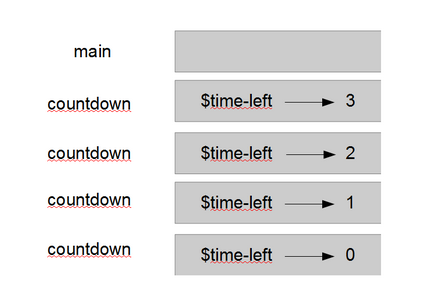
\includegraphics[scale=0.6]{figs/stack2.png}}
\caption{Stack diagram.}
\label{fig.stack2}
\end{figure}


As usual, the top of the stack is the frame for the main 
program.
It is empty because we did not create any variables in 
it or pass any arguments to it.
\index{base case}
\index{recursion!base case}

The four {\tt countdown} frames have different values for the
parameter {\tt \$time-left}.  The bottom of the stack, where {\tt \$time-left = 0}, is
called the {\bf base case}.  It does not make a recursive call, so
there are no more frames.

As an exercise, draw a stack diagram for \verb"print-n-times" 
called with
\verb"$sentence = 'Hello'" and {\tt \$n = 2}.
Then write a function called \verb"do-n-times" that takes a function
and a number, {\tt \$num}, as arguments, and that calls
the given function {\tt \$num} times.
\label{do_n_times}

Solution: see Section~\ref{sol_do_n_times}


\section{Infinite Recursion}
\index{infinite recursion}
\index{recursion!infinite}
\index{runtime error}


If a recursion never reaches a base case, it goes on making
recursive calls forever, and the program never terminates.  This is
known as {\bf infinite recursion}, and it is generally not
a good idea. In fact, your program will not actually execute 
forever but will die at some point when the computer runs out of 
memory or some other critical resource.

You have to be careful when writing recursive subroutines. 
Make sure that you have a base case, and make sure that 
you are guaranteed to reach it. Actually, although this is not 
absolutely required by the language, I would advise you to 
take the good habit of treating the base case first.


\section{Keyboard Input}
\index{keyboard input}

The programs we have written so far accept no input from 
the user. They just do the same thing every time. Raku 
provides built-in functions that stop the program and
wait for the user to type something. 

For example, the {\tt prompt} function prompts the user with 
a question or an instruction. When the user presses 
{\sf Return} or {\sf Enter}, the program resumes and 
\verb"prompt" returns what the user typed as a string 
(without the newline character corresponding to the 
{\sf Return} key typed by the user):
\index{prompt function}
\index{function!prompt}

\begin{verbatim}
my $user = prompt "Please type in your name: ";
say "Hello $user";
\end{verbatim}
%

This is probably one of the most common ways to obtain 
interactive user input, because it is usually a good idea 
to tell the user what is expected.

Another possibility is to use the {\tt get} method (which
 reads a single line) on standard input:
\index{get function}
\index{function!get}

\begin{verbatim}
say "Please type in your name: ";
my $user = $*IN.get;
say "Hello $user";
\end{verbatim}
%
or the {\tt get} function, which reads a line from standard 
input by default:
\begin{verbatim}
say "Please type in your name: ";
my $user = get;
say "Hello $user";
\end{verbatim}
%

\section{Program Arguments and the MAIN Subroutine}
\label{MAIN}
\index{MAIN}

There is another (and often better) way to have a program 
use varying input defined by the user, which is to pass 
command-line arguments to the program, just as we have 
passed arguments to our subroutines.

The easiest way to retrieve arguments passed to a program is 
to use a special subroutine named \verb'MAIN'. A program that 
has a defined \verb'MAIN' subroutine will call automatically  
that subroutine and the command-line arguments supplied 
to the program will be passed as arguments to \verb'MAIN'. 
The \verb'MAIN' signature will enable you to 
retrieve the arguments provided in the command line and 
possibly also check their validity.
\index{signature}

For example, the {\tt greet.pl6} program might look like 
this:
\begin{verbatim}
sub MAIN (Str $name) {
    say "Hello $name";
}
\end{verbatim}

You may call this program twice with different command-line 
arguments as follows:

\begin{verbatim}
$ raku greet.pl6 Larry
Hello Larry

$ raku greet.pl6 world
Hello world
\end{verbatim}

It is very easy to change the argument, since all you need 
to do at the operating system command line is use the up arrow 
and edit the end of the previous command line.

If you forget to supply the argument (or provide the wrong 
number of arguments, or arguments not matching the signature), 
the program will die and Raku will nicely generate and 
display a usage method:

\begin{verbatim}
$ raku greet.pl6
Usage:
  greet.pl6 <name>
\end{verbatim}


\section{Debugging}
\label{whitespace}
\index{debugging}
\index{traceback}

When a syntax or runtime error occurs, the error message contains
a lot of information, but it can be overwhelming.  The most
useful parts are usually:

\begin{itemize}

\item What kind of error it was

\item Where it occurred

\end{itemize}

Syntax errors are usually easy to find, but there are a few
gotchas. In general, error messages indicate where the problem 
was discovered, but the actual error might be earlier in 
the code, sometimes on a previous line or even many lines 
before.
\index{multiplication tables}

For example, the goal of the following code was to display the 
multiplication tables:

\begin{verbatim}
# WARNING: faulty code
sub multiplication-tables {
    for 1..10 -> $x {
        for 1..10 -> $y {
            say "$x x $y\t= ", $x * $y;
        say "";
    }
}

multiplication-tables();
\end{verbatim}

It failed at compilation with the following error:

\begin{verbatim}
$ raku mult_table.pl6
===SORRY!=== Error while compiling /home/Laurent/mult_table.pl6
Missing block (taken by some undeclared routine?)
at /home/Laurent/mult_table.pl6:9
------> multiplication-tables();<HERE><EOL>
\end{verbatim}

The error message reports an error on line~9 of the program 
(the last line of the code), at the end of the line, but 
the actual error is a missing closing brace after line~4 
and before line~5. The reason for this is that, while the 
programmer made the mistake on line~4, the Raku interpreter 
could not detect this error before it reached the 
end of the program. The correct program for displaying 
multiplication tables might be:

\begin{verbatim}
sub multiplication-tables {
    for 1..10 -> $x {
        for 1..10 -> $y {
            say "$x x $y\t= ", $x * $y;
        }
        say "";
    }
}
multiplication-tables();
\end{verbatim}

When an error is reported on the last line of a program, 
it is quite commonly due to a missing closing parenthesis, 
bracket, brace, or quotation mark several lines earlier. 
An editor with syntax highlighting can sometimes help you.
\index{syntax!highlighting}

\index{error!runtime}
\index{runtime error}

The same is true of runtime errors. Consider this program 
aimed at computing 360 degrees divided successively by 
the integers between 2 and 5:

\begin{verbatim}
# WARNING: faulty code
my ($a, $b, $c, $d) = 2, 3, 5;
my $value = 360;
$value /= $_ for $a, $b, $c, $d;
say $value;
\end{verbatim}

This programs compiles correctly but displays a warning and 
then an exception on runtime:

\begin{verbatim}
Use of uninitialized value of type Any in numeric context 
in block  at product.pl6 line 3
Attempt to divide 12 by zero using div
  in block <unit> at product.pl6 line 4
\end{verbatim}
%

The error message indicates a ``division by zero'' exception 
on line~4, but there is nothing wrong with that line. 
The warning on line~3 might give us a clue that the 
script attempts to use an undefined value, but the real error 
is on the first line of the script, where one of the four 
necessary integers (4) was omitted by mistake from the list 
assignment.

\index{division by zero}
\index{uninitialized value}

You should take the time to read error messages carefully, 
but don't assume they point to the root cause of the 
exception; they often point to subsequent problems.


\section{Glossary}

\begin{description}

\item[Integer division] An operation, denoted {\tt div}, 
that divides two numbers and rounds down (toward zero) the 
result to an integer.
  \index{integer division} 
  \index{division!integer}

\item[Modulo operator]  An operator, denoted with a percent sign
({\tt \%}), that works on integers and returns the remainder when one
number is divided by another.
\index{modulo operator}
\index{operator!modulo}

\item[Boolean expression]  An expression whose value is either 
{\tt True} or {\tt False}.
\index{Boolean expression}
\index{expression!Boolean}

\item[Relational operator] One of the operators that compares
its operands. The most common numeric relational operators are 
{\tt ==}, {\tt !=}, {\tt >}, {\tt <}, {\tt >=}, and {\tt <=}. 
The equivalent string relational operators are {\tt eq}, {\tt ne}, 
{\tt gt}, {\tt lt}, {\tt ge}, and {\tt le}.

\item[Logical operator] One of the operators that combines Boolean
expressions: {\tt and}, {\tt or}, and {\tt not}. The equivalent 
higher-precedence operators are {\tt \&\&}, {\tt ||}, and {\tt !}

\item[Conditional statement]  A statement that controls the 
flow of execution depending on some condition.
\index{conditional!statement}
\index{statement!conditional}

\item[Condition] The boolean expression in a conditional 
statement that determines which branch runs.
\index{condition}

\item[Branch] One of the alternative sequences of statements in
a conditional statement.
\index{branch}

\item[Chained conditional]  A conditional statement with a 
series of alternative branches.
\index{chained conditional}
\index{conditional!chained}

\item[Nested conditional]  A conditional statement that appears
in one of the branches of another conditional statement.
\index{nested conditional}
\index{conditional!nested}

\item[Statement modifier] A postfix conditional expression, i.e., 
a conditional expression (using for example {\tt if}, {\tt unless} or 
{\tt for}) that is placed after the statement the executions of which 
it controls. It can also refer to a postfix looping expression.
\index{statement modifier}

\item[Return statement] A statement that causes a function to
end immediately and return to the caller.

\item[Recursion]  The process of calling the function that is
currently executing.
\index{recursion}

\item[Base case]  A conditional branch in a
recursive function that does not make a recursive call.
\index{base case}

\item[Infinite recursion]  A recursion that doesn't have a
base case, or never reaches it.  Eventually, an infinite 
recursion causes a runtime error, for which you may not want 
to wait because it may take a long time.
\index{infinite recursion}

\end{description}

\section{Exercises}
%

\begin{exercise}
%
Using the integer division and the modulo operators:
\index{modulo operator}
\index{operator!mod}
\index{mod, modulo operator}
\index{integer division}
\index{operator!div}
\index{div operator}
\label{int_div_modulo}

\begin{enumerate}

\item Write a subroutine that computes how many days, hours, minutes and seconds there are in the number of seconds passed as an argument to the subroutine.

\item Write a script that computes how many days, hours, minutes and seconds there are in 240,000 seconds.

\item Change your script to compute the number of days, hours, minutes and seconds there are in a number of seconds entered by the script user when prompted to give a number of seconds.

\end{enumerate}

Solutions: Subsection~\ref{sol_int_div_modulo}.

\end{exercise}


\begin{exercise}
\index{Fermat's Last Theorem}
\label{fermat_ex}

Fermat's Last Theorem says that there are no positive integers
$a$, $b$, and $c$ such that

\[ a^n + b^n = c^n \]
%
for any values of $n$ greater than 2.

\begin{enumerate}

\item Write a function named \verb"check-fermat" that takes four
parameters---{\tt a}, {\tt b}, {\tt c}, and {\tt n}---and
checks to see if Fermat's theorem holds.  If
$n$ is greater than 2 and 

\[a^n + b^n = c^n \]
%
the program should print, ``Holy smokes, Fermat was wrong!''
Otherwise the program should print, ``No, that doesn't work.''

\item Write a function that prompts the user to input values
for {\tt a}, {\tt b}, {\tt c}, and {\tt n}, converts them to
integers, and uses \verb"check-fermat" to check whether they
violate Fermat's theorem.
\end{enumerate}

Solution: \ref{sol_fermat_ex}


\end{exercise}


\begin{exercise}
\index{triangle}
\label{triangle}

If you are given three sticks, you may or may not be able to arrange
them in a triangle.  For example, if one of the sticks is 12 inches
long and the other two are one inch long, you will
not be able to get the short sticks to meet in the middle.  For any
three lengths, there is a simple test to see if it is possible 
to form a triangle:

\begin{quotation}
If any of the three lengths is greater than the sum of the other
  two, then you cannot form a triangle.  Otherwise, you
  can.  (If the sum of two lengths equals the third, they form
    what is called a ``degenerate'' triangle.)
\end{quotation}

\begin{enumerate}

\item Write a function named \verb"is-triangle" that takes three
positive numbers as arguments, and that prints either 
``Yes'' or ``No,'' depending on whether you can 
form a triangle from sticks with the given lengths.

\item Write a function that prompts the user to input 
three stick lengths and uses \verb"is-triangle" to check 
whether sticks with the given lengths can form a triangle.

\end{enumerate}

Solution: \ref{sol_triangle}


\end{exercise}

\begin{exercise} 
\index{Fibonacci!numbers}
\label{fibonacci}
The Fibonacci numbers were invented by Leonardo Fibonacci 
(a.k.a. Leonardo of Pisa or simply Fibonacci), an Italian 
mathematician of the thirteenth century.
\index{Fibonacci, Leonardo}

The Fibonacci numbers are a sequence of numbers such as:

\[1, \;1, \;2, \;3, \;5, \;8, \;13, \;21, \;34, \ldots\]
%
in which the first two numbers are equal to 1 and each 
subsequent number of the sequence is defined as the sum of 
the previous two (for example, $5 = 2 + 3$, $8 = 3 + 5$, etc.).

In mathematical notation, the Fibonacci numbers could be defined by recurrence as follows:

\[F_1 = 1, \;F_2 = 1, \;\;and\;\;  F_n = F_{n-1} + F_{n-2} \]
%
\begin{enumerate}

\item Write a program using a {\tt for} loop that prints on screen the first 20 Fibonacci numbers.

\item Write a program which prompts the user to enter a number 
$n$ and, using a {\tt for} loop, computes and displays the 
$n^{th}$ Fibonacci number.

\end{enumerate}

Solution: \ref{sol_fibonacci}


\end{exercise}

\begin{exercise}
\label{sub_recurse}
\index{recursion}

What is the output of the following program?
Draw a stack diagram that shows the state of the program
when it prints the result.

\begin{verbatim}[fontshape=up]
sub recurse($n, $s) {
    if ($n == 0) {
        say $s;
    } else {
        recurse $n - 1, $n + $s;
    }
}
recurse 3, 0;
\end{verbatim}

\begin{enumerate}

\item What would happen if you called the function like 
this: {\tt recurse(-1, 0)}?

\item Write a documentation comment (maybe in the form of a multiline comment) that explains everything someone would need to know in order to use this function (and nothing else).

\end{enumerate}

Solution: \ref{sol_sub_recurse}

\end{exercise}





\chapter{Fruitful Subroutines}
\label{fruitchap}

Most of the Raku functions we have used, such as the math
functions, produce return values.  But most of the subroutines 
we've written so far are void: they have an effect, like 
printing a value, but they don't have a return value.  In
this chapter you will learn to write fruitful functions.


\section{Return Values}
\index{return!value}

Calling a fruitful function generates a return value, 
which we usually assign to a variable or use as part 
of an expression:

\begin{verbatim}
my $pi = 4 * atan 1;
my $height = $radius * sin $radians;
\end{verbatim}
%
Many of the subroutines we have written so far are void.  
Speaking casually, they have no usable return value; more 
precisely, their return value may be {\tt Any}, {\tt Nil}, 
{\tt ()}, or {\tt True}.

In this chapter, we are (finally) going to write fruitful subroutines.
The first example is {\tt area}, which returns the area of a circle
with the given radius:

\begin{verbatim}
sub area($radius) {
    my $circular_area = pi * $radius**2;
    return $circular_area;
}
\end{verbatim}
%
We have seen the {\tt return} statement before, but in a fruitful
function the {\tt return} statement includes
an expression.  This statement means: ``Return immediately from
this function and use the following expression as a return value.''
The expression can be arbitrarily complicated, so we could
have written this function more concisely:
\index{return!statement}
\index{statement!return}

\begin{verbatim}
sub area($radius) {
    return pi * $radius**2;
}
\end{verbatim}
%
On the other hand, {\bf temporary variables} like 
\verb'$circular_area' can make debugging easier. They 
may also help document what is going on.
\index{temporary variable}
\index{variable!temporary}

Sometimes it is useful to have multiple return statements, for 
example one in each branch of a conditional:

\begin{verbatim}
sub absolute_value($num){
    if $num < 0 {
        return -$num;
    } else {
        return $num;
    }
}
\end{verbatim}
%
Since these {\tt return} statements are in an alternative 
conditional, only one runs.

This could also be written more concisely using the statement 
modifier syntax:

\begin{verbatim}
sub absolute_value($num){
    return -$num if $num < 0;
    return $num;
}
\end{verbatim}
%
Here again, only one of the return statements runs: if the 
number is negative, the first return statement is executed and 
the subroutine execution stops there; if the number is 
positive or zero, then only the second return statement is 
executed. 

As soon as a return statement runs, the function
terminates without executing any subsequent statements.
Code that appears after an unconditional {\tt return} statement, 
or any other place the flow of execution can never reach, 
is called {\bf dead code}.
\index{dead code}

In a fruitful function, it is a good idea to ensure
that every possible path through the program hits a
{\tt return} statement.  For example:

\begin{verbatim}
# WARNING: faulty code
sub absolute_value($num){
    if $num < 0 {
        return -$num;
    } 
    if $num > 0 {
        return $num;
    }
}
\end{verbatim}
%


This subroutine is incorrect because if {\tt \$num} happens to be 0,
neither condition is true, and the subroutine ends without hitting a
{\tt return} statement.  If the flow of execution gets to the end
of a function, the return value is {\tt ()}, which basically 
means ``not defined'' and is clearly not the absolute value of 0:
\index{undefined value}

\begin{verbatim}
> absolute_value(0)
()
\end{verbatim}
%
By the way, Raku provides a built-in function called 
{\tt abs} that computes absolute values.
\index{abs function or method}
\index{function!abs}

\label{compare}
As an exercise, write a {\tt compare} subroutine that 
takes two numbers, {\tt \$x} and {\tt \$y}, and returns {\tt 1} 
if {\tt \$x > \$y}, {\tt 0} if {\tt \$x == \$y}, and 
{\tt -1} if {\tt \$x < \$y}.

Solution: \ref{sol_compare}
\index{compare function}
\index{function!compare}


\section{Incremental Development}
\label{incremental.development}
\index{development plan!incremental}
\index{incremental development}

As you write larger functions, you might find yourself
spending more time debugging.

To deal with increasingly complex programs,
you might want to try a process called
{\bf incremental development}.  The goal of incremental development
is to avoid long debugging sessions by adding and testing only
a small amount of code at a time.
\index{testing!incremental development}
\index{Pythagorean theorem}

As an example, suppose you want to find the distance between 
two points, given by the Cartesian or rectangular coordinates 
$(x_1, y_1)$ and $(x_2, y_2)$. By the Pythagorean theorem, 
the distance is:
\index{Pythagorean theorem}
\index{Cartesian coordinates}
\index{coordinates!Cartesian}
\index{rectangular!coordinates}
\index{coordinates!rectangular}


\begin{displaymath}
\mathrm{distance} = \sqrt{(x_2 - x_1)^2 + (y_2 - y_1)^2}
\end{displaymath}
%
The first step is to consider what a {\tt distance} function should
look like in Raku.  In other words, what are the inputs (parameters)
and what is the output (return value)?

In this case, the inputs are two points, which you can represent
using four numbers.  The return value is the distance represented by
a numeric value.

Immediately you can write an outline of the function:

\begin{verbatim}
sub distance($x1, $y1, $x2, $y2) {
    return 0.0;
}
\end{verbatim}
%
Obviously, this version doesn't compute distances; it always returns
zero.  But it is syntactically correct, and it runs, which means that
you can test it before you make it more complicated.

To test the new function, call it with sample arguments:

\begin{verbatim}
> distance(1, 2, 4, 6);
0.0
\end{verbatim}
%
I chose these values so that the horizontal distance is 3 and the
vertical distance is 4; that way, the result is 5, the hypotenuse 
of a 3-4-5 triangle. When testing a function, it is
useful to know the right answer.
\index{testing!knowing the answer}

At this point we have confirmed that the function is syntactically
correct, and we can start adding code to the body.
A reasonable next step is to find the differences
$x_2 - x_1$ and $y_2 - y_1$.  The next version stores those values in
temporary variables and prints them:

\begin{verbatim}
sub distance($x1, $y1, $x2, $y2) {
    my $dx = $x2 - $x1;
    my $dy = $y2 - $y1;
    say '$dx is ', $dx;
    say '$dy is ', $dy;
    return 0.0;
}
\end{verbatim}
%
If the function is working, it should display \verb"$dx is 3" and 
\verb"$dy is 4" (and still return 0.0).  If so, we know that the 
function is getting the right arguments and performing the 
first computation correctly.  If not, there are only a few lines 
to check.

Next we compute the sum of squares of {\tt \$dx} and {\tt \$dy}:

\begin{verbatim}
sub distance($x1, $y1, $x2, $y2) {
    my $dx = $x2 - $x1;
    my $dy = $y2 - $y1;
    my $dsquared = $dx**2 + $dy**2;
    say '$dsquared is: ', $dsquared;
    return 0.0;
}
\end{verbatim}
%
Again, you would run the program at this stage and check the output
(which should be 25).
Finally, you can use the {\tt sqrt} built-in function to compute 
and return the result:
\index{sqrt function}
\index{function!sqrt}

\begin{verbatim}
sub distance($x1, $y1, $x2, $y2) {
    my $dx = $x2 - $x1;
    my $dy = $y2 - $y1;
    my $dsquared = $dx**2 + $dy**2;
    my $result = sqrt $dsquared;
    return $result;
}
\end{verbatim}
%
If that works correctly, you are done.  Otherwise, you might
want to print the value of {\tt \$result} before the return
statement.

The final version of the subroutine doesn't display anything when it
runs; it only returns a value.  The {\tt print} statements we wrote
are useful for debugging, but once you get the function working, you
should remove them.  Code like that is sometimes called 
{\bf scaffolding} because it is helpful for building the program 
but is not part of the final product.
\index{scaffolding}

When you start programming, you should add only a line or two of code at a
time.  As you gain more experience, you might find yourself writing
and debugging bigger chunks.  Either way, incremental development
can save you a lot of debugging time.

The key aspects of the process are:

\begin{enumerate}

\item Start with a working program and make small incremental changes. 
At any point, if there is an error, you should have a good idea
where it is.

\item Use variables to hold intermediate values so you can
display and check them.

\item Once the program is working, you might want to remove some of
the scaffolding or consolidate multiple statements into compound
expressions, but only if doing so does not make the program 
difficult to read.

\end{enumerate}

Note that, at least for relatively simple cases, you can also 
use the REPL to test expressions and even multiline statements 
or subroutines in interactive mode before you commit them to your 
program code. This is usually fast and can save you some time.
\index{REPL}
\index{interactive mode}

\label{hypotenuse}
As an exercise, use incremental development to write a function
called {\tt hypotenuse} that returns the length of the hypotenuse of a
right triangle given the lengths of the other two legs as arguments.
Record each stage of the development process as you go.

Solution: \ref{sol_hypotenuse}.
\index{hypotenuse}



\section{Composition}
\index{composition}
\index{function composition}

As you should expect by now, you can call one function from within
another.  As an example, we'll write a function that takes two points,
the center of the circle and a point on the perimeter, and computes
the area of the circle.

Assume that the center point is stored in the variables {\tt \$x-c} and
{\tt \$y-c}, and the perimeter point is in {\tt \$x-p} and {\tt \$y-p}. The
first step is to find the radius of the circle, which is the distance
between the two points.  We just wrote a function, {\tt
distance}, that does that:

\begin{verbatim}
my $radius = distance($x-c, $y-c, $x-p, $y-p);
\end{verbatim}
%
The next step is to find the area of a circle with that radius;
we just wrote that, too:

\begin{verbatim}
my $result = area($radius);
\end{verbatim}
%
Encapsulating these steps in a function, we get:
\index{encapsulation}

\begin{verbatim}
sub circle-area($x-c, $y-c, $x-p, $y-p) {
    my $radius = distance($x-c, $y-c, $x-p, $y-p);
    my $result = area($radius);
    return $result;
}
\end{verbatim}
%
The temporary variables {\tt \$radius} and {\tt \$result} are useful for
development and debugging, but once the program is working, we can
make it more concise by composing the function calls:

\begin{verbatim}
sub circle-area($x-c, $y-c, $x-p, $y-p) {
    return area distance($x-c, $y-c, $x-p, $y-p);
}
\end{verbatim}
%

The last line of the previous example now works like a data 
pipeline from right to left: the \verb'distance' function 
takes the four arguments and returns a distance (the radius) 
which is fed as an argument to the \verb'area'; with this 
argument, \verb'area' is now able to return the area, which 
is then returned by \verb'circle-area' to the caller code. 
We'll come back later to this very expressive data pipeline 
model.
\index{pipe-line programming}

\section{Boolean Functions}
\label{boolean}

Functions can return Boolean values, which is often convenient for hiding
complicated tests inside functions. For example:
\index{Boolean function} 

\begin{verbatim}
sub is-divisible(Int $x, Int $y) {
    if $x % $y == 0 {
        return True;
    } else {
        return False;
    }
}
\end{verbatim}
%
It is common to give Boolean functions names that sound like yes/no
questions; \verb"is-divisible", for instance, returns either 
{\tt True} or {\tt False} to indicate whether {\tt x} is 
divisible by {\tt y}.

Here is an example:

\begin{verbatim}
> is-divisible(6, 4);
False
> is-divisible(6, 3);
True
\end{verbatim}
%
The result of the {\tt ==} operator is a Boolean value, so we 
can write the subroutine more concisely by returning it directly:

\begin{verbatim}
sub is-divisible(Int $x, Int $y) {
    return $x % $y == 0
}
\end{verbatim}
%
If there is no return statement, a Raku subroutine returns the 
value of expression on the last code line of the subroutine 
(provided the last code line is an expression that gets evaluated), so that the 
{\tt return} statement is not required here. In addition, 
since 0 is a false value and any other integer a true value, 
this could be further rewritten as follows:
\begin{verbatim}
sub is-divisible(Int $x, Int $y) { 
    not $x % $y 
}
\end{verbatim}

The {\tt Int} type declarations in the subroutine signatures above 
are not necessary. The subroutine would work without them, but 
they can provide some form of protection against using this 
subroutine with faulty arguments.

Boolean functions are often used in statement modifiers:
\index{statement modifier}
\index{modifier!statement}

\begin{verbatim}
say "$x is divisible by $y" if is-divisible($x, $y);
\end{verbatim}
%
It might be tempting to write something like:

\begin{verbatim}
say "$x is divisible by $y" if is-divisible($x, $y) == True;
\end{verbatim}
%
But the extra comparison is unnecessary: {\tt is-divisible} 
returns a Boolean value that can be interpreted directly by
the {\tt if} conditional.

\label{isbetween}
As an exercise, write a function \verb"is-between(x, y, z)" that
returns {\tt True} if $x \le y \le z$ or {\tt False} otherwise.

Solution: \ref{sol_isbetween}.

\section{A Complete Programming Language}

We've seen in the section above several ways of writing a 
subroutine to check the divisibility of two integers.
\index{divisibility}

In fact, as briefly mentioned earlier, Raku has a 
``is divisible'' operator, \verb'%%', which returns 
{\tt True} if the number on the left is divisible by 
the one on the right:
%\index{%%!is divisible operator}
\index{is divisible operator}

\begin{verbatim}
> 9 %% 3
True
> 9 %% 4
False
\end{verbatim}

So there was no need to write the {\tt is-divisible} subroutine. 
But don't worry, that's all right if you did not remember that. 
Speakers of natural languages are allowed to have different 
skill levels, to learn as they go and to put the language 
to good use before they know the whole language. The same 
is true with Raku. You (and I) don't know all about Raku 
yet, just as we don't know all of English. But it is in fact 
``Officially Okay in the Perl and Raku Culture'' to use the subset of 
the language that you know. You are in fact 
encouraged to use what is sometimes called ``baby Perl'' or ``baby Raku'' 
to write programs, even if they are somewhat clumsy at the 
beginning. That's the best way of learning Raku, just as using 
``baby talk'' is the right way for a child to learn English.
\index{baby Perl}
\index{Perl culture}
\index{baby Raku}
\index{Raku culture}

The number of different ways of accomplishing a given task, 
such as checking whether one number is divisible 
by another, is an example of one of Perl's and Raku's mottos: 
\emph{there is more than 
one way to do it}, oft abbreviated TIMTOWTDI. Some ways may be 
more concise or more efficient than others, but, in the Perl and Raku 
philosophy, you are perfectly entitled to do it your way, 
especially if you're a beginner, provided you find the correct 
result.
\index{there is more than one way to do it}
\index{TIMTOWTDI}
\index{Turing!complete language}
\index{language!Turing complete}
\index{Turing, Alan}
\index{Turing!thesis}

We have only covered a small subset of Raku so far, but you 
might be interested to know that this subset is a {\em complete}
programming language, which means that essentially anything 
that can be computed can be expressed in this language.  
Any program ever written could be rewritten using only the 
language features you have learned so far (actually, you 
would need a few commands to control devices like the mouse, 
disks, networks, etc., but that's all).

Proving that claim is a nontrivial exercise first accomplished by Alan
Turing, one of the first computer scientists (some would argue that he
was a mathematician, but a lot of early computer scientists started as
mathematicians).  Accordingly, it is known as the Turing Thesis.
For a more complete (and accurate) discussion of the Turing Thesis,
I recommend Michael Sipser's book {\em Introduction to the
Theory of Computation}.

\section{More Recursion}
\label{more.recursion}
\index{recursion}


To give you an idea of what you can do with the tools you have learned
so far, we'll evaluate a few recursively defined mathematical
functions.  A recursive definition is similar to a circular
definition, in the sense that the definition contains a reference to
the thing being defined.  A truly circular definition is not very
useful:

\begin{description}

\item[Vorpal] An adjective used to describe something that is vorpal.
\index{vorpal}
\index{circular definition}
\index{definition!circular}

\end{description}

If you saw that definition in the dictionary, you might be annoyed. On
the other hand, if you looked up the definition of the factorial
function, denoted with the symbol $!$, you might get something like
this:
%
\begin{eqnarray*}
&&  0! = 1 \\
&&  n! = n (n-1)!
\end{eqnarray*}
%
This definition says that the factorial of 0 is 1, and the 
factorial of any other (positive integer) value, $n$, is 
$n$ multiplied by the factorial of $n-1$.

So $3!$ is 3 times $2!$, which is 2 times $1!$, which is 1 times
$0!$. Putting it all together, $3!$ equals 3 times 2 times 1 times 1,
which is 6.
\index{factorial!function}
\index{function!factorial}
\index{recursive definition}

If you can write a recursive definition of something, you can
write a Raku program to evaluate it. The first step is to decide
what the parameters should be.  In this case it should be clear
that {\tt factorial} takes a number\footnote{It should really be an 
integer, but we'll get back to that later in this chapter.}:

\begin{verbatim}
sub factorial($n){
}
\end{verbatim}
%
If the argument happens to be 0, all we have to do is return 1:

\begin{verbatim}
sub factorial($n){
    if $n == 0 {
        return 1;
    }
}   
\end{verbatim}
%
Otherwise, and this is the interesting part, we have to make a
recursive call to find the factorial of $n-1$ and then 
multiply it by $n$:
\index{factorial!using recursion}

\begin{verbatim}
sub factorial($n){
    if $n == 0 {
        return 1;
    } else {
        my $recurse = factorial($n-1);
        my $result = $n * $recurse;
        return $result;
    }
}
\end{verbatim}
%
The flow of execution for this program is similar to the flow of {\tt
countdown} in Section~\ref{recursion}.  If we call {\tt factorial}
with the value 3:

Since 3 is not 0, we take the second branch and calculate the factorial
of {\tt \$n-1}...

\begin{quote}
Since 2 is not 0, we take the second branch and calculate the factorial of
{\tt \$n-1}...


  \begin{quote}
  Since 1 is not 0, we take the second branch and calculate the factorial
  of {\tt \$n-1}...


    \begin{quote}
    Since 0 equals 0, we take the first branch and return 1
    without making any more recursive calls.
    \end{quote}


  The return value, 1, is multiplied by \verb'$n', which is 1, and the
  result is returned.
  \end{quote}


The return value, 1, is multiplied by \verb'$n', which is 2, and the
result is returned.
\end{quote}


The return value, 2, is multiplied by \verb'$n', which is 3, and 
the result, 6, becomes the return value of the subroutine call 
that started the whole process.
\index{stack diagram}

Figure~\ref{fig.stack3} shows what the stack diagram looks like for
this sequence of function calls.

\begin{figure}
\centerline
{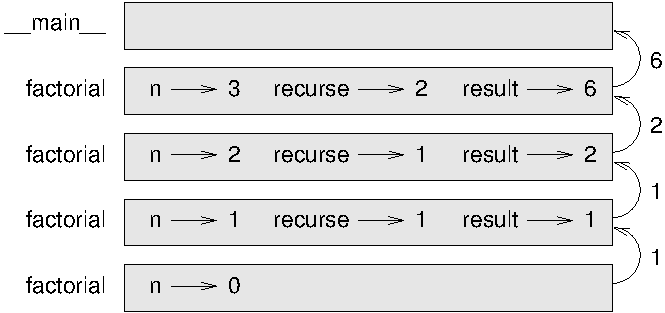
\includegraphics[scale=0.8]{figs/stack3.pdf}}
\caption{Stack diagram.}
\label{fig.stack3}
\end{figure}

The return values are shown being passed back up the stack.  In each
frame, the return value is the value of {\tt \$result}, which is the
product of {\tt \$n} and {\tt \$recurse}.
\index{function!frame}
\index{frame}

In the last frame, the local
variables {\tt \$recurse} and {\tt \$result} do not exist, because
the branch that creates them does not run.

A seasoned Raku programmer might write a more concise or
more idiomatic subroutine\footnote{We will see later even 
more idiomatic ways of computing the factorial of a number.}:
\index{idiomatic}

\begin{verbatim}
sub factorial($n){
    return 1 if $n == 0;
    return $n * factorial $n-1;
}
\end{verbatim}
%
This is not better than our initial version, and will probably 
not run significantly faster, but this is arguably clearer, 
at least once you get used to this type of syntax.

\section{Leap of Faith}
\index{recursion}
\index{leap of faith}

Following the flow of execution is one way to read programs, but
it can quickly become overwhelming.  An alternative is what may 
be called the ``leap of faith.''  When you come to a
subroutine call, instead of following the flow of execution, you {\em
assume} that the subroutine works correctly and returns the right
result.

In fact, you are already practicing this leap of faith when you use
built-in functions.  When you call math functions such as {\tt cos} or {\tt sqrt},
you don't examine the bodies of those functions.  You just
assume that they work because the people who wrote the built-in
functions were likely to be good programmers (and because you 
can safely assume that they have been thoroughly tested).

The same is true when you call one of your own subroutines.  For
example, in Section~\ref{boolean}, we wrote a subroutine called 
\verb"is-divisible" that determines whether one number is divisible by
another.  Once we have convinced ourselves that this subroutine is
correct---by examining the code and testing---we can use the subroutine without looking at the body again.
\index{testing!leap of faith}

The same is true of recursive programs.  When you get to the recursive
call, instead of following the flow of execution, you should assume
that the recursive call works (returns the correct result) and then ask
yourself, ``Assuming that I can find the factorial of \verb"$n-1", can I
compute the factorial of \verb"$n"?''  It is clear that you
can, by multiplying by \verb"$n".

Of course, it's a bit strange to assume that the subroutine works
correctly when you haven't finished writing it, but that's why
it's called a leap of faith!


\section{One More Example}
\label{one.more.example}

\index{Fibonacci!function}
\index{function!Fibonacci}
After {\tt factorial}, the most common example of a recursively
defined mathematical function is {\tt fibonacci}, which has the
following definition (see
  \url{http://en.wikipedia.org/wiki/Fibonacci_number}):
%
\begin{eqnarray*}
&& \mathrm{fibonacci}(0) = 1 \\
&& \mathrm{fibonacci}(1) = 1 \\
&& \mathrm{fibonacci}(n) = \mathrm{fibonacci}(n-1) + \mathrm{fibonacci}(n-2)
\end{eqnarray*}
%

In plain English, a Fibonacci sequence is a sequence of numbers 
such as:
\begin{verbatim}
1, 1, 2, 3, 5, 8, 13, 21, ...
\end{verbatim}
where the two first terms are equal to 1 and any other term is the 
sum of the two preceding ones.

We briefly covered the Fibonacci sequence in Exercise~\ref{fibonacci} 
of the previous chapter and implemented it with a {\tt for} loop.

Let's now translate the recursive definition into Raku. It looks like this:

\begin{verbatim}
sub fibonacci ($n) {
    return 1 if $n == 0 or $n == 1;
    return fibonacci($n-1) + fibonacci($n-2)
}
\end{verbatim}
%
If you try to follow the flow of execution here, even for fairly
small values of \verb'$n', your head explodes.  But according to the
leap of faith, if you assume that the two recursive calls
work correctly, then it is clear that you get
the right result by adding them together.
\index{flow of execution}


\section{Checking Types}
\label{guardian}

What happens if we call {\tt factorial} and give it 1.5 as an argument?
\index{type!checking}
\index{error checking}
\index{factorial!function}

It seems that we get an infinite recursion.  How can that be? 
The subroutine has a base case---when {\tt \$n == 0}.  But if {\tt \$n} 
is not an integer, we can {\em miss} the base case and recurse forever.
\index{infinite recursion}
\index{recursion!infinite}
\index{base case}

In the first recursive call, the value of {\tt \$n} is 0.5.
In the next, it is -0.5.  From there, it gets smaller
(more negative), but it will never be 0.

We have two choices.  We can try to generalize the {\tt factorial}
function to work with noninteger numbers, or we can make 
{\tt factorial} check its argument.  The first option is 
called the gamma function and it's a little beyond the scope 
of this book.  So we'll go for the second.
\index{function!gamma}
\index{gamma function}

We have already seen examples of subroutines using the signature 
to verify the type of the argument. So we can add the {\tt Int} 
type to the parameter in the signature. While we're at it, 
we can also make sure the argument is positive or zero:

\begin{verbatim}
sub factorial(Int $n where $n >= 0){
    return 1 if $n == 0;
    return $n * factorial $n-1;
}
\end{verbatim}
%
\index{constraint}
\index{trait}
The {\tt Int} type checking in the signature handles 
nonintegers, this is not new. The {\tt where \$n >= 0} 
part is a parameter constraint: if the parameter is negative, 
the subroutine should fail.  Technically, the constraint is 
implemented here within the signature using a syntax feature 
called a \emph{trait}, that is a property imposed on the 
parameter at compile time. If the argument passed to the 
function is not an integer or if it is negative, the program prints
an error message to indicate that something went wrong:

\begin{verbatim}
> say factorial 1.5
Type check failed in binding $n; expected Int but got Rat
  in sub factorial at <unknown file> line 1
  in block <unit> at <unknown file> line 1

> say factorial -3
Constraint type check failed for parameter '$n'
> say factorial "Fred"
Type check failed in binding $n; expected Int but got Str
  in sub factorial at <unknown file> line 1
  in block <unit> at <unknown file> line 1
\end{verbatim}
% 
If we get past both checks, we know that \verb'$n' is an 
integer and that it is positive or zero, so we can prove 
that the recursion terminates.


\index{subset!type}
\index{type subset}
Another way to achieve a similar result is to define your own 
subset of the built-in types. For example, you can create an 
{\tt Even-int} subset of integers and then use it more or less 
as if it were a new type for declaring your variables or 
typing your subroutine parameters:

\begin{verbatim}
subset Even-int of Int where { $_ %% 2 } # or : … where { $_ % 2 == 0 }
# Even-int can now be used as a type

my Even-int $x = 2; # OK
my Even-int $y = 3; # Type mismatch error
\end{verbatim}

Similarly, in the case of the {\tt factorial} subroutine, we 
can create a \emph{nonnegative integer} subset and use it 
for checking the parameter passed to the subroutine:

\begin{verbatim}
subset Non-neg-int of Int where { $_ >= 0}
# ...

sub factorial(Non-neg-int $n){
    return 1 if $n == 0;
    return $n * factorial $n-1;
}
\end{verbatim}
%
If we pass a negative integer to the subroutine, we get 
a similar error as before:

\begin{verbatim}
Constraint type check failed for parameter '$n'...
\end{verbatim}

\index{guardian pattern}
\index{pattern!guardian}
This program demonstrates a pattern sometimes called a {\bf guardian}.
The signature acts as a guardian, protecting the code that
follows from values that might cause an error.  The guardians make it
possible to prove the correctness of the code.


\section{Multi Subroutines}
\label{multisubs}
\index{multi!subroutine}

It is possible to write multiple versions of a subroutine 
with the same name but with different signatures, for example  
a different \emph{arity} (a fancy word for the number of 
arguments) or different argument types, using the 
{\tt multi} keyword. In this case, the interpreter will 
pick the version of the subroutine whose signature 
matches (or best matches) the argument list. This process 
is called \emph{dispatch}. Dispatch happens depending on 
the number (arity), type and name of arguments.
\index{arity}
\index{dispatch (multi subroutines)}
\index{multi!dispatch}

For example, we could rewrite the factorial function 
as follows:
\index{factorial!using multi subroutines}

\begin{verbatim}
multi sub fact(0) { 1 };
multi sub fact(Int $n where $n > 0) {
    $n * fact $n - 1;
}
say fact 0;   # -> 1
say fact 10;  # -> 3628800
\end{verbatim}

Here, we don't enter into infinite recursion because, when 
the parameter passed to {\tt fact} is 0, it is the first 
version of the multi subroutine that is called and it returns 
an integer value (1), and this ends the recursion.

Similarly, the Fibonacci function can be rewritten with 
multi subroutines:
\index{Fibonacci!function with multi subroutines}

\begin{verbatim}
multi fibonacci(0) { 1 }
multi fibonacci(1) { 1 }
multi fibonacci(Int $n where $n > 1) { 
    fibonacci($n - 2) + fibonacci($n - 1) 
}
say fibonacci 10;  # -> 89
\end{verbatim}

Note that in the {\tt fibonacci} example just above, we have 
omitted the {\tt sub} keyword, since it isn't necessary after 
the {\tt multi} declarator.

Many built-in functions and most operators of Raku are 
written as multi subroutines.

In the two examples above, only one of the {\tt multi} 
subroutine signature could match the input parameters. 
For example, if the argument passed to the {\tt fact} 
subroutine is 0, then the first version is called; 
if the argument is greater than 0, then the second version 
is called.

What if more that one signature matches the passed 
arguments? Then, the dispatch process becomes a little 
bit more complicated. As said at the beginning of this section, 
the runtime environment will select the \emph{candidate} 
subroutine that \emph{best} matches the signature. 
In such cases, the run time environment first looks 
at the arity (number of arguments) of the signature. 
If only one signature matches the number of parameters 
passed to the subroutine, then it is this candidate subroutine 
that is selected. If, on the other hand, several signatures 
match the number of arguments, then the type of the arguments 
drives the dispatch. \footnote{We will see later 
(see section \ref{named_parameters}) that there can 
be other types of signatures, with \emph{named parameters}. 
Let's just say here that, when there are named arguments, 
they drive the dispatch even when their type is the same as 
another candidate. \index{named parameter}
}  
\index{arity}
\index{dispatch (multi subroutines)}
\index{multi!dispatch}
\index{candidate (multi subroutines)}
\index{multi!subroutine}



\section{Debugging}
\label{factdebug}

Breaking a large program into smaller functions or subroutines 
creates natural checkpoints for debugging.  If a subroutine 
is not working, there are three possibilities to consider:
\index{debugging} 

\begin{itemize}

\item There is something wrong with the arguments the subroutine
is getting; a precondition is violated.

\item There is something wrong with the subroutine; a postcondition
is violated.

\item There is something wrong with the return value or the
way it is being used.

\end{itemize}

To rule out the first possibility, you can add a print statement
at the beginning of the function and display the values of the
parameters (and maybe their types).  Or you can write code
that checks the preconditions explicitly.
\index{precondition}
\index{postcondition}

For the purpose of debugging, it is often useful to print 
the content of a variable or of a parameter within a string 
with surrounding characters, so that you may visualize 
characters that are otherwise invisible, such as spaces or 
newlines. For example, you think that the \verb'$var' should 
contain ``two,'' and run the following test:
\begin{verbatim}
if $var eq "two" {
    do-something()
}
\end{verbatim}
%
But it fails and the {\tt do-something} subroutine is never called.

Perhaps you want to use a print statement that will ascertain 
the content of \verb'$var':
\begin{verbatim}
say "[$var]";
if $var eq "two" {
    do-something()
}
\end{verbatim}
%

This might print:
\begin{verbatim}
[two ]
\end{verbatim}
%

or:
\begin{verbatim}
[two
]
\end{verbatim}
%
Now, you know that the equality test fails because \verb'$var'
contains a trailing character (space or newline) that might otherwise 
be difficult to detect.

If the parameters look good, add a {\tt print} statement before each
{\tt return} statement and display the return value.  If
possible, check the result by hand.  Consider calling the
function with values that make it easy to check the result
(as in Section~\ref{incremental.development}).

If the function seems to be working, look at the function call
to make sure the return value is being used correctly (or used
at all!).
\index{flow of execution}

Adding print statements at the beginning and end of a function
can help make the flow of execution more visible.
For example, here is a version of {\tt factorial} with
print statements:
\index{factorial!recursive function with debug statements}

\begin{verbatim}
sub factorial(Int $n) {
    my $space = ' ' x (4 * $n);
    say $space, 'factorial ', $n;
    if $n == 0 {
        say $space, 'returning 1';
        return 1;
    } else {
        my $result = $n * factorial $n-1;
        say $space, 'returning ', $result;
        return $result;
    }
}
\end{verbatim}
%
The {\tt \$space} variable is a string of space characters that controls the
indentation of the output.  Here is the result of {\tt factorial(4)} :

\begin{verbatim}
                factorial 4
            factorial 3
        factorial 2
    factorial 1
factorial 0
returning 1
    returning 1
        returning 2
            returning 6
                returning 24
\end{verbatim}
%
If you are confused about the flow of execution, this kind of
output can be helpful.  It takes some time to develop effective
scaffolding, but a bit of scaffolding can save a lot of debugging.


\section{Glossary}

\begin{description}

\item[Temporary variable]  A variable used to store an intermediate value in
a complex calculation.
\index{temporary variable}
\index{variable!temporary}

\item[Dead code]  Part of a program that can never run, often because
it appears after a {\tt return} statement.
\index{dead code}

\item[Incremental development]  A program development plan intended to
avoid debugging by adding and testing only
a small amount of code at a time.
\index{incremental development}

\item[Scaffolding]  Code that is used during program development but is
not part of the final version.
\index{scaffolding}

\item[Guardian]  A programming pattern that uses a conditional
statement to check for and handle circumstances that
might cause an error.
\index{guardian pattern}
\index{pattern!guardian}

\end{description}


\section{Exercises}

\begin{exercise}

Draw a stack diagram for the following program.  What does 
the program print? Please try to answer these questions before 
trying to run the program.
\index{stack diagram}

\begin{verbatim}[fontshape=up]
sub b(Int $z) {
    my $prod = a($z, $z);
    say $z, " ", $prod;
    return $prod;
}
sub a(Int $x is copy, Int $y) {
    $x++;
    return $x * $y;
}
sub c(Int $x, Int $y, Int $z) {
    my $total = $x + $y + $z;
    my $square = b($total) ** 2;
    return $square;
}

my $x = 1;
my $y = $x + 1;
say c($x, $y + 3, $x + $y);
\end{verbatim}

\end{exercise}


\begin{exercise}
\label{ackermann}
\index{Ackermann function}

The Ackermann function, $A(m, n)$, is defined as follows:

\begin{eqnarray*}
A(m, n) = \begin{cases} 
              n+1 & \mbox{if } m = 0 \\ 
        A(m-1, 1) & \mbox{if } m > 0 \mbox{ and } n = 0 \\ 
A(m-1, A(m, n-1)) & \mbox{if } m > 0 \mbox{ and } n > 0.
\end{cases} 
\end{eqnarray*}
%
See \url{http://en.wikipedia.org/wiki/Ackermann_function}.
Write a subroutine named {\tt ack} that evaluates the Ackermann function.
Use your subroutine to evaluate {\tt ack(3, 4)}, which should be 125.
What happens for larger values of {\tt m} and {\tt n}?

Solution: \ref{sol_ackermann}.
\index{Ackermann function}
\index{function!ack}

\end{exercise}


\begin{exercise}
\label{palindrome}
\index{palindrome}

A palindrome is a word that is spelled the same backward and
forward, like ``noon'' and ``redivider.''  Recursively, a word
is a palindrome if the first and last letters are the same
and the middle is a palindrome.
\index{palindrome}

The following are subroutines that take a string argument and
return the first, last, and middle letters:

\begin{verbatim}[fontshape=up]
sub first_letter(Str $word){
    return substr $word, 0, 1;
}

sub last_letter(Str $word){
    return substr $word, *-1, 1;
}

sub middle_letter(Str $word){
    return substr $word, 1, *-1;
}
\end{verbatim}
%
Don't worry about how they work for the time being; we will see 
that in Chapter~\ref{strings} on strings. For now:

\begin{enumerate}

\item Type these subroutines into a file named {\tt palindrome.raku}
and test them out.  What happens if you call \verb'middle_l' with
a string with two letters?  One letter?  What about the empty
string, which is written \verb"''" and contains no letters? 
Given that the {\tt .chars} method returns the length of a 
string, how could you add a signature constraint to reject invalid input?

\item Write a subroutine called \verb"is-palindrome" that takes
a string argument and returns {\tt True} if it is a palindrome
and {\tt False} otherwise.  Remember that you can use the
built-in method {\tt .chars} to check the length of a string.

\end{enumerate}

Solution: \ref{sol_palindrome}.
\index{palindrome}

\end{exercise}

\begin{exercise}
\index{power}
\label{power}

An integer number, $a$, is a power of $b$ if it is divisible by $b$
and $a/b$ is a power of $b$.  Write a function called
\verb"is-power-of" that takes parameters {\tt a} and {\tt b}
and returns {\tt True} if {\tt a} is a power of {\tt b}.
Note: you will have to think about the base case.
\index{base case}

Solution: \ref{sol_power}

\end{exercise}


\begin{exercise}
\index{greatest common divisor (GCD)}
\index{GCD (greatest common divisor)}
\label{gcd}
\index{gcd function}

The greatest common divisor (GCD) of $a$ and $b$ is the largest number
that divides both of them with no remainder.  

One way to find the GCD of two numbers is based on the observation
that if $r$ is the remainder when $a$ is divided by $b$, then $gcd(a,
b) = gcd(b, r)$.  As a base case, we can use $gcd(a, 0) = a$.

Write a function called
\verb"gcd" that takes parameters {\tt a} and {\tt b}
and returns their greatest common divisor.

Credit: this exercise is based on an example from Abelson and
Sussman's {\em Structure and Interpretation of Computer Programs}.
\index{Abelson, Harold}
\index{Sussman, Gerald Jay}

Solution: \ref{sol_gcd}

\end{exercise}




\chapter{Iteration}
\label{iteration}

This chapter is about iteration, which is the ability to run
a block of statements repeatedly.  We saw a kind of iteration,
using recursion, in Section~\ref{recursion}.
We saw another kind, using a {\tt for} loop,
in Section~\ref{for_loops}.  In this chapter we'll see yet another
kind, using a {\tt while} statement.
But first we want to say a little more about variable assignment.

\section{Assignment Versus Equality}
\index{assignment!operator}
\index{equality operator}

Before going further, I want to address a common source of confusion.
Because Perl uses the equals sign ({\tt =}) for assignment, it is
tempting to interpret a statement like {\tt \$a = \$b} as a
mathematical proposition of equality, that is, the claim that 
{\tt \$a} and {\tt \$b} are equal.  But this interpretation is 
wrong.
\index{equality and assignment}

First, equality is a symmetric relationship and assignment is not.  For
example, in mathematics, if $a=7$ then $7=a$.  But in Perl, the
statement {\tt \$a = 7} is legal and {\tt 7 = \$a} is not.

Also, in mathematics, a proposition of equality is either true or
false for all time.  If $a=b$ now, then $a$ will always equal $b$.
In Perl, an assignment statement can make two variables equal, but
they don't have to stay that way:

\begin{verbatim}
> my $a = 5;
5
> my $b = $a;   # $a and $b are now equal
5
> $a = 3;       # $a and $b are no longer equal
3
> say $b;
5
\end{verbatim}
%
The third line changes the value of {\tt \$a} but does not 
change the value of {\tt \$b}, so they are no longer equal. 

In brief, remember that {\tt =} is an assignment operator and  
not an equality operator; the operators for testing equality 
between two terms are {\tt ==} for numbers and {\tt eq} for strings.

\section{Reassignment}
\index{assignment}
\index{statement!assignment}
\index{reassignment}

As you may have discovered, it is legal to make more than one
assignment to the same variable.  A new assignment makes an existing
variable refer to a new value (and stop referring to the old value):

\begin{verbatim}
> my $x = 5;
5
> say $x;
5
> $x = 7;
7
> say $x
7
\end{verbatim}
%
The first time we display 
{\tt \$x}, its value is 5; the second time, its
value is 7.

Figure~\ref{fig.assign2} shows what {\bf reassignment} looks
like in a state diagram. \index{state diagram} \index{diagram!state}

Reassigning variables is often useful, but you should use this feature 
with some caution.  If the values of variables change frequently, it can
make the code difficult to read and debug.

\begin{figure}
\centerline
{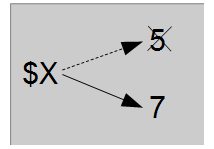
\includegraphics[scale=0.5]{figs/reassignment.png}}
\caption{State diagram.}
\label{fig.assign2}
\end{figure}



\section{Updating Variables}
\label{update}

\index{update}
\index{variable!updating}

A common kind of reassignment is an {\bf update},
where the new value of the variable depends on the old:

\begin{verbatim}
> $x = $x + 1;
\end{verbatim}
%
This means ``get the current value of {\tt \$x}, add one, and then
update {\tt \$x} with the new value.''

If you try to update a variable that has not been given a value, 
you get a warning, because Perl evaluates the right side 
of the assignment statement before it assigns a value to {\tt \$x}:

\begin{verbatim}
> my $x;
> $x = $x + 1;
Use of uninitialized value of type Any in numeric context 
 in block <unit> at <unknown file> line 1
\end{verbatim}
%
Before you can update a variable, you have to declare it and 
{\bf initialize} it, usually with an assignment statement:
\index{initialization (before update)}

\begin{verbatim}
> my $x = 0;
> $x = $x + 1;
\end{verbatim}
%
Updating a variable by adding 1 is called an {\bf increment};
subtracting 1 is called a {\bf decrement}.
\index{increment operator}
\index{decrement operator}

As mentioned earlier in Section~\ref{expr_and_statements}, 
Perl has some shortcuts for increment and decrement :

\begin{verbatim}
$x += 1; # equivalent to $x = $x + 1
$x++;    # also equivalent 

$x -= 1; # equivalent to $x = $x - 1
$x--;    # also equivalent 
\end{verbatim}

\section{The {\tt while} Statement}
\index{statement!while}
\index{while loop}
\index{loop!while}
\index{iteration}

Computers are often used to automate repetitive tasks.  Repeating
identical or similar tasks without making errors is something that
computers do well and people do poorly.  In a computer program,
repetition is also called {\bf iteration}.

We have already seen two functions, {\tt countdown} and
\verb"print-n-times", that iterate using recursion 
(see Section~\ref{recursion}).  Because 
iteration is so common, most programming languages including 
Perl provide language features to make it easier.
One is the {\tt for} statement we saw in Section~\ref{for_loops}.
We'll get back to that later.

Another is the {\tt while} statement.  Here is a version of {\tt
countdown} that uses a {\tt while} statement:

\begin{verbatim}
sub countdown(Int $n is copy) {
    while $n > 0 {
        say $n;
        $n--;
    }
    say 'Blastoff!';
}
\end{verbatim}
%
You can almost read the {\tt while} statement as if it were English.
It means, ``While {\tt \$n} is greater than 0,
display the value of {\tt n} and then decrement
{\tt \$n}.  When you get to 0, display the word {\tt Blastoff!}''
\index{flow of execution}

More formally, here is the flow of execution for a {\tt while} statement:

\begin{enumerate}

\item Determine whether the condition is true or false.

\item If false, exit the {\tt while} statement
and continue execution at the next statement.

\item If the condition is true, run the
body and then go back to step 1.

\end{enumerate}

This type of flow is called a loop because the third step
loops back around to the top.  
\index{condition}
\index{loop}
\index{body}

The body of the loop should change the value of one or more variables
so that the condition becomes false eventually and the loop
terminates.  Otherwise, the loop will repeat forever, which is called
an {\bf infinite loop}.  An endless source of amusement for computer
scientists is the observation that the directions on shampoo,
``Lather, rinse, repeat,'' are an infinite loop.
\index{infinite loop}
\index{loop!infinite}

In the case of {\tt countdown}, we can prove that the loop
terminates: if {\tt \$n} is zero or negative, the loop never runs.
Otherwise, {\tt \$n} gets smaller each time through the
loop, so eventually we have to get to 0.

For some other loops, it is not so easy to tell whether the 
loop terminates.  For example:

\begin{verbatim}
sub sequence($n is copy) {
    while $n != 1 {
        say $n;
        if $n %% 2 {        # $n is even
            $n = $n / 2;
        } else {            # $n is odd
            $n = $n*3 + 1
        }
    }
    return $n;
}
\end{verbatim}
%
The condition for this loop is {\tt \$n != 1}, so the loop will continue
until {\tt \$n} is {\tt 1}, which makes the condition false.

Each time through the loop, the program outputs the value of {\tt \$n}
and then checks whether it is even or odd.  If it is even, {\tt \$n} is
divided by 2.  If it is odd, the value of {\tt \$n} is replaced with
{\tt \$n*3 + 1}. For example, if the argument passed to {\tt sequence}
is 42, the resulting values of {\tt n} are 42, 21, 64, 32, 16, 8, 4, 2, 1.

Since {\tt \$n} sometimes increases and sometimes decreases, there is no
obvious proof that {\tt \$n} will ever reach 1, or that the program
terminates.  For some particular values of {\tt n}, we can prove
termination.  For example, if the starting value is a power of two,
{\tt n} will be even every time through the loop
until it reaches 1. The previous example ends with such a sequence
of powers of two, starting with 64.
\index{Collatz conjecture}

The hard question is whether we can prove that this program terminates
for {\em all} positive values of {\tt n}.  So far, no one has
been able to prove it {\em or} disprove it!  (See
\url{http://en.wikipedia.org/wiki/Collatz_conjecture}.)

As an exercise, you might want to rewrite the function 
\verb"print-n-times" from Section~\ref{recursion} using 
iteration instead of recursion.

\index{statement modifier}
\index{postfix!syntax}
The {\tt while} statement can also be used as a statement modifier (or postfix syntax):

\begin{verbatim}
my $val = 5;
print $val while $val-- > 0;   # prints 43210
print "\n";
\end{verbatim}

The {\tt while} loop statement executes the block as long as 
its condition is true. There is also an {\tt until} loop 
statement, which executes the block as long as its condition 
is false:
\index{until loop}

\begin{verbatim}
my $val = 1;
until $val > 5 {
    print $val++;              # prints 12345
}
print "\n";
\end{verbatim}

\section{Local Variables and Variable Scoping}

We have seen in Section~\ref{localvar} that variables created 
within a subroutine (with the {\tt my} keyword) are \emph{local} 
to that subroutine. The {\tt my} 
keyword if often called a \emph{declarator}, because it 
is used for declaring a new variable (or other identifier). 
It is by far the most common declarator. Other declarators 
include {\tt our} or {\tt state}, briefly described later 
in this chapter. 
\index{lexical scope}
\index{lexical variable}
\index{variable!lexical}
\index{my}
\index{declarator}

Similarly, subroutine 
parameters are also usually \emph{local} to the subroutine 
in the signature of which they are declared.
\index{subroutine parameters}

We briefly mentioned that the term \emph{lexically scoped} 
is probably more accurate than local, but it was 
too early at that point to really explain what this means.

Declaring a variable with {\tt my} gives it \emph{lexical 
scope}. This means it only exists within the current block. 
Loosely speaking, a 
block is a piece of Perl code within curly brackets or 
braces. For example, the body of a subroutine and the code of a 
{\tt while} or {\tt for} loop or of an {\tt if} conditional
statement are code blocks. Any variable created with the 
{\tt my} declarator exists and is available for use only 
between the place where it is declared and the end of the 
enclosing code block.
\index{bracket!curly}
\index{curly bracket}

For example, this code:

\begin{verbatim}
if $condition eq True {
    my $foo = "bar";
    say $foo;  # prints "bar"
}
say $foo;      # ERROR: "Variable '$foo' is not declared ..."
\end{verbatim}
%
will fail on the second print statement, because the \verb'say' 
function call is not in 
the lexical scope of the {\tt \$foo} variable, which ends 
with the closing brace of the condition block. If we want 
this variable to be accessible after the end of the condition, 
then we would need to declare it before the {\tt if} statement. 
For example:

\begin{verbatim}
my $foo;
if $condition eq True {
    $foo = "bar";
    say $foo;  # prints "bar"
} else {
    $foo = "baz";
}
say $foo;      # prints "bar" or "baz" depending on $condition
\end{verbatim}
%
If a lexical variable is not declared within a block, its 
scope will extend until the end of the file (this is sometimes 
called a static or a global variable, although these terms are 
somewhat inaccurate). For example, in the last code snippet 
above, the scope of the {\tt \$foo} variable will extend 
until the end of the file, which may or may not be a good thing, 
depending on how you intend to use it. It 
is often better to reduce the scope of variables as much as 
possible, because this helps reduce dependencies between 
various parts of the code and limits 
the risk of subtle bugs. In the code above, if we want to 
limit the scope of {\tt \$foo}, we could add braces to create 
an enclosing block for the sole purpose of limiting the scope:
\begin{verbatim}
{
    my $foo;
    if $condition eq True {
        $foo = "bar";
        say $foo;  # prints "bar"
    } else {
        $foo = "baz";
    }
    say $foo;      # prints "bar" or "baz" depending on $condition
}
\end{verbatim}
% 
Now, the outer braces create an enclosing block limiting the 
scope of {\tt \$foo} to where we need it. This may seem to be a 
somewhat contrived example, but it is not uncommon to add 
braces only for the purpose of precisely defining the scope 
of something.

Lexical scoping also means that variables with the same names
can be temporarily redefined in a new scope: 

\begin{verbatim}
my $location = "outside";
sub outer {
    say $location;
}
sub inner {
    my $location = "inside";
    say $location;
}
say $location;   # -> outside
outer();         # -> outside
inner();         # -> inside
say $location;   # -> outside
\end{verbatim}
% 
We have in effect two variables with the same name, 
{\tt \$location}, but different scopes. One is valid only 
within the {\tt inner} subroutine where it has been redefined, 
and the other anywhere else.

If we add a new subroutine:
\begin{verbatim}
sub nowhere {
    my $location = "nowhere";
    outer();
}
nowhere();       # -> outside
\end{verbatim}
% 
this will still print ``outside,'' because the {\tt outer} 
subroutine knows about the ``outside'' version of the 
{\tt \$location} variable, which existed when {\tt outer} was defined.
In other word, the {\tt outer} code that referenced to the 
outer variable (``outside'') knows about the variable that existed 
when it was created, but not about the variable existing where 
it was called. This is how \emph{lexical} variables work. 
This behavior is the basis for building \emph{closures}, a  
form of subroutine with some special properties that we 
will study later in this book, but 
is in fact implicitly present everywhere in Perl~6.
\index{closure}
\index{variable!lexical}
\index{lexical variable}

While having different variables with the same name can give 
you a lot of expressive power, we would 
advise you to avoid creating different variables with the 
same name and different scopes, at least until you really understand 
these concepts well enough to know what you are doing, as this 
can be quite tricky.

By far, most variables used in Perl are lexical variables, 
declared with the {\tt my} declarator. Although they are 
not declared with {\tt my}, parameters declared 
in the signature of subroutines and parameters of pointy 
blocks also have a lexical scope limited to the body of the 
subroutine or the code block.
\index{my}
\index{declarator}

There are other declarators, such as {\tt our}, which creates 
a package-scoped variable, and {\tt state}, which creates a 
lexically scoped variable but with a persistent value. They 
are relatively rarely used.
\index{our}
\index{state}

One last point: although they are usually not declared with 
a {\tt my} declarator, subroutines themselves also have by default
a lexical scope. If they are defined within a block, they will 
be seen only within that block. An example of this has been 
given at the end of the solution to the GCD exercise of the 
previous chapter (see Subsection~\ref{sol_gcd}). 
That being said, you \emph{can} declare a subroutine with 
with a {\tt my} declarator if you wish:

\begin{verbatim}
my sub frobnicate { 
    # ... 
}
\end{verbatim}

This technique might add some consistency or some form of 
self-documenting feature, but you won't buy very much 
added functionality with that.
 

\section{Control Flow Statements ({\tt last}, {\tt next}, etc.)}
\index{control flow}
\index{flow!control}
\index{last statement}
\index{statement!last}
\index{next statement}
\index{statement!next}

Sometimes you don't know it's time to end a loop until you get half
way through the body.  In that case, you can use a control flow 
statement such as {\tt last} to jump out of the loop.

For example, suppose you want to take input from the user until they
type {\tt done}.  You could write:

\begin{verbatim}
while True {
    my $line = prompt "Enter something ('done' for exiting)\n";
    last if $line eq "done";
    say $line;
}
say 'Done!';
\end{verbatim}
%
The loop condition is {\tt True}, which is always true, so the
loop runs until it hits the {\tt last} statement.

Each time through, it prompts the user to type something.
If the user types {\tt done}, the {\tt last} statement exits
the loop.  Otherwise, the program echoes whatever the user types
and goes back to the top of the loop.  Here's a sample run:

\begin{verbatim}
$ perl6 while_done.pl6
Enter something ('done' for exiting)
Not done
Not done
Enter something ('done' for exiting)
done
Done!
\end{verbatim}
%
This way of writing {\tt while} loops is common because you
can check the condition anywhere in the loop (not just at the
top) and you can express the stop condition affirmatively
(``stop when this happens'') rather than negatively (``keep 
going until that happens'').

Using a {\tt while} loop with a condition that is always true 
is a quite natural way of writing an infinite loop, i.e., a 
loop that will run forever until something else in the code 
(such as the {\tt last} statement used above) forces the 
program to break out of the loop. This is commonly used in 
many programming languages, and this works well in Perl. There 
is, however, another common and more idiomatic way of constructing 
infinite loops in Perl~6: using the {\tt loop} statement, 
which we will study in Section~\ref{C-style loop} 
(p.~\pageref{C-style loop}). For now, we'll use the {\tt while True} 
statement, which is fairly legitimate.
\index{idiomatic}
\index{loop!infinite}
\index{infinite loop}

Sometimes, rather than simply breaking out of the {\tt while}  loop 
as with the {\tt last} control statement, you need to start the 
body of the loop at the beginning. For example, you may want 
to check whether the user input is correct with some 
(unspecified) {\tt is-valid} subroutine before processing 
the data, and ask the user to try again if the input was not 
correct. In this case, the {\tt next} control statement lets 
you start at the top the loop body again:
\index{next statement}
\index{statement!next}

\begin{verbatim}
while True {
    my $line = prompt "Enter something ('done' for exiting)\n";
    last if $line eq "done";
    next unless is-valid($line);
    # further processing of $line;
}
print('Done!')
\end{verbatim}
%
Here, the loop terminates if the user types ``done.'' If not, the user input is checked by the {\tt is-valid} subroutine; if the subroutine returns a true value, the processing continues forward; if it returns a false value, then the control flow starts again at the beginning of the body of the loop, so the user is prompted again to submit a valid input.

The {\tt last} and {\tt next} control statements also work in 
{\tt for} loops. For example, the following {\tt for} loop 
iterates in theory on a range of integer numbers between 1 and 20, 
but discards odd numbers by virtue of a {\tt next} statement 
and breaks out of the loop with a {\tt last} statement as 
soon as the loop variable is greater than {\tt \$max} (i.e., 10 in this  example):
\index{for loop}
\index{loop!for}
\index{statement!for}

\begin{verbatim}
my $max = 10;
for 1..20 -> $i {
    next unless $i %% 2; # keeps only even values
    last if $i > $max;   # stops loop if $i is greater than $max
    say $i;              # prints 2 4 6 8 10
}
\end{verbatim}

You may have as many {\tt last} and {\tt next} statements as you 
like, just as you may have as many {\tt return} statements as 
you like in a subroutine. Using such control flow statements 
is not considered poor 
practice. During the early days of structured programming, 
some people insisted that loops and subroutines have only one 
entry and one exit. The one-entry notion is still a good idea, 
but the one-exit notion has led people to bend over backwards 
and write a lot of unnatural code. Much of programming consists of traversing 
decision trees. A decision tree naturally starts with a single 
trunk but ends with many leaves. Write your code with the number 
of loop controls (and subroutine exits) that is natural to the 
problem you're trying to solve. If you've declared your variables 
with reasonable scopes, everything gets automatically cleaned up 
at the appropriate moment, no matter how you leave the block.


\section{Square Roots}
\label{squareroot}
\index{square root}

Loops are often used in programs that compute
numerical results by starting with an approximate answer and
iteratively improving it.
\index{Newton's method}

For example, one way of computing square roots is Newton's 
method (also known as the Newton-Raphson's method).
Suppose that you want to know the square root of $a$.  If you start
with almost any estimate, $x$, you can compute a better
estimate $y$ with the following formula:

\[ y = \frac{x + a/x}{2} \]
%
For example, if $a$ is 4 and $x$ is 3:

\begin{verbatim}
> my $a = 4;
4
> my $x = 3;
3
> my $y = ($x + $a/$x)/2;
2.166667
\end{verbatim}
%
The result is closer than 3 to the correct answer 
($\sqrt{4} = 2$) .  If we repeat the process with the new estimate, it gets even closer:

\begin{verbatim}
> $x = $y;
2.166667
> $y = ($x + $a/$x)/2;
2.006410
\end{verbatim}
%
After a few more updates, the estimate is almost exact:
\index{update}

\begin{verbatim}
> $x = $y;
2.006410
> $y = ($x + $a/$x)/2;
2.000010
> $x = $y;
2.000010
> $y = ($x + $a/$x)/2;
2.000000000026
\end{verbatim}
%
In general we don't know ahead of time how many steps it takes
to get to the right answer, but we know when we get there
because the estimate stops changing:

\begin{verbatim}
> $x = $y;
2.000000000026
> $y = ($x + $a/$x)/2;
2
> $x = $y;
2
> $y = ($x + $a/$x)/2;
2
\end{verbatim}
%
When {\tt \$y == \$x}, we can stop.  Here is a loop that starts
with an initial estimate, {\tt x}, and improves it until it
stops changing:

\begin{verbatim}
my ($a, $x) = (4, 3);
while True {
    say "-- Intermediate value: $x";
    my $y = ($x + $a/$x) / 2;
    last if $y == $x;
    $x = $y;
}
say "Final result is $x";
\end{verbatim}
%
This will print:
\begin{verbatim}
-- Intermediate value: 3
-- Intermediate value: 2.166667
-- Intermediate value: 2.006410
-- Intermediate value: 2.000010
-- Intermediate value: 2.000000000026
-- Intermediate value: 2
Final result is 2
\end{verbatim}
%

For most values of {\tt \$a} this works fine, but there are a 
couple of caveats with this approach. First, in most programming 
languages, it is dangerous to test {\tt float} equality, because 
floating-point values are only approximately right. We do not 
have this problem with Perl~6, because, as we have already 
mentioned, it is using a better representation of rational 
numbers than most generalist programming languages. (You 
may want to keep this in mind if you are using some other
languages.) Even if we don't have this problem with Perl, there 
may also be some problems with algorithms that do not behave 
as well as Newton's algorithm. For example, some algorithms 
might not converge as fast and as neatly as Newton's algorithm but might instead produce alternate values above and below the accurate result.
\index{floating-point}
\index{epsilon}

Rather than checking whether {\tt \$x} and {\tt \$y} are exactly equal, it
is safer to use the built-in function {\tt abs} to compute the
absolute value, or magnitude, of the difference between them:

\begin{verbatim}
    last if abs($y - $x) < $epsilon:
\end{verbatim}
%
where \verb"epsilon" has a very small value like {\tt 0.0000001} 
that determines how close is close enough.



\section{Algorithms}
\index{algorithm}

Newton's method is an example of an {\bf algorithm}: it is a
mechanical process for solving a category of problems (in this
case, computing square roots).

To understand what an algorithm is, it might help to start with
something that is not an algorithm.  When you learned to multiply
single-digit numbers, you probably memorized the multiplication table.
In effect, you memorized 100 specific solutions.  That kind of
knowledge is not algorithmic.

But if you were ``lazy,'' you might have learned a few
tricks.  For example, to find the product of $n$ and 9, you can
write $n-1$ as the first digit and $10-n$ as the second
digit.  (For example, to figure out $9*7$, $n-1$ is 6 and 
$10-n$ is 3, so that the product $9*7$ is 63.) This trick 
is a general solution for multiplying any single-digit 
number by 9.  That's an algorithm!
\index{addition with carrying}
\index{carrying, addition with}
\index{subtraction!with borrowing}
\index{borrowing, subtraction with}

Similarly, the techniques you learned in school for addition 
(with carrying), subtraction (with borrowing), and long 
division are all algorithms.  One
of the characteristics of algorithms is that they do not require any
intelligence to carry out.  They are mechanical processes where
each step follows from the last according to a simple set of rules.

Executing algorithms is boring, but designing them is interesting,
intellectually challenging, and a central part of computer science.

Some of the things that people do naturally, without difficulty or
conscious thought, are the hardest to express algorithmically.
Understanding natural language is a good example.  We all do it, but
so far no one has been able to explain {\em how} we do it, at least
not in the form of an algorithm.


\section{Debugging}
\label{bisectbug}

As you start writing bigger programs, you might find yourself
spending more time debugging.  More code means more chances to
make an error and more places for bugs to hide.
\index{debugging!by bisection}
\index{bisection, debugging by}

One way to cut your debugging time is ``debugging by bisection.''
For example, if there are 100 lines in your program and you
check them one at a time, it would take 100 steps.

Instead, try to break the problem in half.  Look at the middle
of the program, or near it, for an intermediate value you
can check.  Add a {\tt say} statement (or something else
that has a verifiable effect) and run the program.

If the midpoint check is incorrect, there must be a problem in the
first half of the program.  If it is correct, the problem is
in the second half.

Every time you perform a check like this, you halve the number of
lines you have to search.  After six steps (which is fewer than 100),
you would be down to one or two lines of code, at least in theory.

In practice it is not always clear what
the ``middle of the program'' is and not always possible to
check it.  It doesn't make sense to count lines and find the
exact midpoint.  Instead, think about places
in the program where there might be errors and places where it
is easy to put a check.  Then choose a spot where you
think the chances are about the same that the bug is before
or after the check.


\section{Glossary}

\begin{description}

\item[Reassignment] Assigning a new value to a variable that
already exists.
\index{reassignment}

\item[Update] An assignment where the new value of the variable
depends on the old.
\index{update}

\item[Initialization] An assignment that gives an initial value to
a variable that may later be updated.
\index{initialization!variable}

\item[Increment] An update that increases the value of a variable
(often by one).
\index{increment operator}

\item[Decrement] An update that decreases the value of a variable.
\index{decrement operator}

\item[Iteration] Repeated execution of a set of statements using
either a recursive function call or a loop.
\index{iteration}

\item[Infinite loop] A loop in which the terminating condition is
never satisfied.
\index{infinite loop}
\index{loop!infinite}

\item[Algorithm]  A general process for solving a category of
problems.
\index{algorithm}

\end{description}


\section{Exercises}

\begin{exercise}
\label{test_sqrt}
\index{square root}
\index{algorithm!square root}

Copy the loop from Section~\ref{squareroot}
and encapsulate it in a subroutine called
\verb"my-sqrt" that takes {\tt \$a} as a parameter, chooses a
reasonable value of {\tt \$x}, and returns an estimate of 
the square root of {\tt \$a}.

To test it, write a function named \verb"test-square-root"
that prints a table like this:

\begin{verbatim}[fontshape=up]
a  mysqrt(a)        sqrt(a)          diff
1  1.0000000000000  1.0000000000000  1.110223e-15
2  1.4142135623747  1.4142135623731  1.594724e-12
3  1.7320508075689  1.7320508075689  0.000000e+00
4  2.0000000000000  2.0000000000000  0.000000e+00
5  2.2360679774998  2.2360679774998  0.000000e+00
6  2.4494897427832  2.4494897427832  8.881784e-16
7  2.6457513110647  2.6457513110646  1.025846e-13
8  2.8284271247494  2.8284271247462  3.189449e-12
9  3.0000000000000  3.0000000000000  0.000000e+00

\end{verbatim}
%
The first column is a number, $a$, the second column is the 
square root of $a$ computed with \verb"my-sqrt", the third 
column is the square root computed by the {\tt sqrt} built-in 
function of Perl, and the fourth column is the absolute value of 
the difference between the two estimates. Don't worry too much about 
obtaining a clean tabular formatting, we haven't 
seen the built-in functions to do that. 

Solution: \ref{sol_test_sqrt}
%

\end{exercise}



\begin{exercise}
\index{Ramanujan, Srinivasa}
\index{Ramanujan, Srinivasa!pi estimate}
\index{pi!estimate}
\label{pi_estimate}

The mathematician Srinivasa Ramanujan found an infinite 
series that can be used to generate a numerical
approximation of $1 / \pi$:
\index{pi}

\[ \frac{1}{\pi} = \frac{2\sqrt{2}}{9801} 
\sum^\infty_{k=0} \frac{(4k)!(1103+26390k)}{(k!)^4 396^{4k}} \]

Write a function called \verb"estimate-pi" that uses this 
formula to compute and return an estimate of $\pi$.  It 
should use a {\tt while} loop to compute terms of the 
summation until the last term is smaller than {\tt 1e-15} 
(which is Perl notation for $10^{-15}$). You can check
the result by comparing it to the built-in constant {\tt pi}.
Solution: \ref{sol_pi_estimate}.

\end{exercise}




\chapter{Strings}
\label{strings}
\index{string}

Strings are not like integers, rationals, and Booleans.  
A string is a {\bf sequence} of characters, which means 
it is an ordered collection of other values, and you 
sometimes need to access to some of these individual 
values.  In this chapter you'll see how to analyze, 
handle, and modify strings, and you'll learn about some 
of the methods strings provide. You will also start to learn about 
a very powerful tool for manipulating text data, regular 
expressions a.k.a. regexes.
\index{sequence}
\index{regex}


\section{A String is a Sequence}

\index{sequence}
\index{character}
\index{bracket operator}
\index{operator!bracket}
A string is primarily a piece of textual data, but it 
is technically an ordered sequence of characters.  

Many programming languages allow you to access individual 
characters of a string with an index between brackets. This 
is not directly possible in Perl, but you still can access 
the characters one at a time using the {\tt comb} built-in 
method and the bracket operator:

\begin{verbatim}
> my $string = "banana";
banana
> my $st = $string.comb;
(b a n a n a)
> say $st[1];
a
> say $st[2];
n
\end{verbatim}
%
The {\tt comb} in the second statement splits the string 
into a list of characters that you can then access 
individually with square brackets.
\index{comb function and method}
\index{method!comb}
\index{function!comb}
\index{bracket!square}
\index{square bracket operator}
\index{index}
\index{subscript}

The expression in brackets is called an {\bf index} 
(it is sometimes also called a subscript).  
The index indicates which character in the sequence you
want (hence the name). But this may not be what you 
expected: the item with index 1 is the second letter of 
the word. For computer scientists, the index is usually 
an offset from the beginning. The offset of the first 
letter (``b'') is zero, and the 
offset of the first ``a'' is 1, not 2, and so on.
\index{index!starting at zero}
\index{zero, index starting at}

You could also retrieve a ``slice'' of several characters in 
one go using the range operator within the brackets:
\index{slice}

\begin{verbatim}
> say $st[2..5]
(n a n a)
\end{verbatim}
%
\index{substring}
Again, the ``nana'' substring starts on the third letter of 
\verb"'banana'", but this letter is indexed 2, and the sixth letter is index 5. 

But, even if all this might be useful at times, this is 
not the way you would usually handle strings in Perl, 
which has higher level tools that are more powerful and more 
expressive, so that you seldom need to use indexes or 
subscripts to access individual characters.

Also, if there is a real need to access and manipulate 
individual letters, it would make more sense to store 
them in an array, but we haven't covered arrays yet, so 
we'll have to come back to that later.


\section{Common String Operators}
\index{string!operators}

Perl provides a number of operators and functions to 
handle strings. Let's review some of the most popular ones.

\subsection{String Length}
\index{chars function}
\index{function!chars}
\index{string!length}

The first thing we might want to know about a string is its length. The {\tt chars} built-in returns the number of characters 
in a string and can be used with either a method or a function 
syntax:
\index{invocation!method}
\index{method invocation}

\begin{verbatim}
> say "banana".chars;   # method invocation syntax
6
> say chars "banana";   # function call syntax
6
\end{verbatim}
%

\index{Unicode}
\index{grapheme}
Note that, with the advent of Unicode, the notion of 
string length has 
become more complicated than it used to be in the era
of ASCII-only strings. Today, a character may be made of one,
two, or more bytes. The {\tt chars} routine returns the 
number of characters (in the sense of Unicode graphemes, which
is more or less what humans perceive as characters) within 
the string, even if some of these characters require an 
encoding over 2, 3, or 4 bytes.

A string with a zero length (i.e., no character) is called 
an \emph{empty string}.

\subsection{Searching For a Substring Within the String}

\label{find}
\index{index function}
\index{function!index}
\index{substring}

The {\tt index} built-in usually takes two arguments, a string 
and a substring (sometimes called the ``haystack'' and the 
``needle''), searches for the substring in the string, and 
returns the position where the substring is found (or an 
undefined value if it wasn't found): 

\begin{verbatim}
> say index "banana", "na";
2
> say index "banana", "ni";
Nil
\end{verbatim}
%

\index{offset}
Here again, the index is an offset from the beginning of the 
string, so that the index of the first letter (``b'') is zero, 
and the offset of the first ``n'' is 2, not 3.
\index{index!starting at zero}

You may also call {\tt index} with a method syntax:
\begin{verbatim}
> say "banana".index("na");
2
\end{verbatim}
%

The {\tt index} function can take a third optional argument, 
an integer indicating where to start the \emph{search} 
(thus ignoring in the search any characters before the 
start position):

\begin{verbatim}
> say index "banana", "na", 3;
4
\end{verbatim}
%
Here, the {\tt index} function started the search on the middle 
``a'' and thus found the position of the second occurrence of 
the ``na'' substring.

\index{function!rindex}
\index{rindex function}
There is also a {\tt rindex} function, which searches the string 
backwards from the end and returns the last position of the 
substring within the string:

\begin{verbatim}
> say rindex "banana", "na";
4
\end{verbatim}
%

Note that even though the {\tt rindex} function searches the 
string backwards (from the end), it returns a position 
computed from the start of the string.

\subsection{Extracting a Substring from a String}
\index{substr function or method}
\index{function!substr}
\index{substring}

The opposite of the {\tt index} function is the {\tt substr} 
function or method, which, given a start position and a length, 
extracts a substring from a string:

\begin{verbatim}
> say substr "I have a dream", 0, 6;
I have
> say "I have a dream".substr(9, 5)
dream
\end{verbatim}
%

\index{chars function}
\index{Unicode}
\index{grapheme}
Note that, just as for the {\tt chars} function, the length 
is expressed in characters (or Unicode graphemes), not in bytes. 
Also, as you can see, spaces separating words within the string 
obviously count as characters. The length argument is optional; 
if it is not provided, the {\tt substr} function returns the 
substring starting on the start position to the end of the string:

\begin{verbatim}
> say "I have a dream".substr(7)
a dream
\end{verbatim}

Similarly, if the length value is too large for the 
substring starting on the start position, the {\tt substr} 
function will also return the substring starting on the start 
position to the end of the string:

\begin{verbatim}
> say substr "banana", 2, 10;
nana
\end{verbatim}

Of course, the start position and length parameters need not be 
hardcoded numbers as in the examples above; you may use a variable 
instead (or even an expression or a function returning a numeric 
value), provided the variable or value can be coerced into an integer. 
But the start position must be within the string range, 
failing which you would obtain a {\tt Start argument to 
substr out of range ...} error; so you may have to verify it 
against the length of the string beforehand. 

You can also start counting backwards from the end of the 
string with the following syntax:

\begin{verbatim}
> say "I have a dream".substr(*-5)
dream
> say substr "I have a dream", *-5;
dream
\end{verbatim}
%

\index{substr function}
\index{substring}

\subsection{A Few Other Useful String Functions or Methods}
\index{string!operators}

This may not be obvious yet, but we will see soon 
that the combination of the above string functions gives you 
already a lot of power to manipulate strings way beyond what 
you may think possible at this point.

Let us just mention very briefly a few additional functions 
that may prove useful at times.

\subsubsection{flip}

\index{flip function}
\index{function!flip}
The {\tt flip} function or method reverses a string:

\begin{verbatim}
> say flip "banana";
ananab
\end{verbatim}
%

\subsubsection{split}
\index{split function or method}
\index{function!split}
\index{delimiter}
The {\tt split} function or method splits a string 
into substrings, based on delimiters found in the string:

\begin{verbatim}
> say $_ for split "-", "25-12-2016";
25
12
2016
> for "25-12-2016".split("-") -> $val {say $val};
25
12
2016
\end{verbatim}

The delimiter can be a single quoted character as in the 
examples above or a string of several characters, such as 
a comma and a space in the example below:

\begin{verbatim}
> .say for split  ', ', "Jan, Feb, Mar";
Jan
Feb
Mar
\end{verbatim}

By default, the delimiters don't appear in the output produced 
by the {\tt split} function or method, but this behavior can 
be changed with the use of an appropriate \emph{adverb}. An adverb 
is basically a named argument to a function that modifies 
the way the function behaves. For example, the {\tt :v} (values) adverb 
tells {\tt split} to also output the value of the delimiters:
\index{adverb}
\index{:v adverb}

\begin{verbatim}
> .perl.say for split  ', ', "Jan, Feb, Mar", :v;
"Jan"
", "
"Feb"
", "
"Mar"
\end{verbatim}

The other adverbs that can be used in this context are 
{\tt :k} (keys), {\tt :kv} (keys and values), and {\tt :p} 
(pairs). Their detailed meaning can be 
found in the documentation for {\tt split} 
(\url{https://docs.perl6.org/routine/split}). The 
{\tt skip-empty} adverb removes empty chunks from the result 
list.

The {\tt split} function can also use a regular expression 
\emph{pattern} as delimiter, and this can make it much more powerful. 
We will study regular expressions later in this chapter.
\index{regular expression}
\index{regex}

\subsubsection{String Concatenation}

\index{concatenate operator}
\index{string!concatenation}
\index{string concatenation}

The \verb'~' operator concatenates two strings into one:

\begin{verbatim}
> say "ban" ~ "ana";
banana
\end{verbatim}
%

You may chain several occurrences of this operator to 
concatenate more than two strings:

\begin{verbatim}
> say "ba" ~ "na" ~ "na";
banana
\end{verbatim}
%

Used as a unary prefix operator,
\verb'~' ``stringifies'' (i.e., transforms into a string) its argument:
\index{stringify operator}
\index{stringification}

\begin{verbatim}
> say (~42).WHAT;
(Str)
\end{verbatim}
%

\subsubsection{Splitting on Words}

\index{words function or method}
The {\tt words} function returns a list of words that make 
up the string:

\begin{verbatim}
> say "I have a dream".words.perl;
("I", "have", "a", "dream").Seq
> .say for "I have a dream".words;
I
have
a
dream
\end{verbatim}
%

\subsubsection{join}

\index{join function or method}
\index{function!join}
The {\tt join} function takes a separator argument and a list 
of strings as arguments; it interleaves them with the separator, 
concatenates everything into a single string, and returns the 
resulting string.

This example illustrates the chained use of the {\tt words} and 
{\tt join} functions or methods:
\begin{verbatim}
say 'I have a dream'.words.join('|');    # -> I|have|a|dream
say join ";", words "I have a dream";    # -> I;have;a;dream
\end{verbatim}
%

\index{words function or method}
In both cases, {\tt words} first splits the original 
string into a list of words, and {\tt join} stitches 
the items of this list back into a new string interleaved 
with the separator.  

\subsubsection{Changing the Case}
\index{lc function or method} 
\index{lower case!lc function}
\index{uc function or method}
\index{tc function or method}
\index{upper case}
\index{lower case}
\index{title case}
\index{case!upper}
\index{case!lower}
\index{case!title}

The {\tt lc} and {\tt uc} routines return respectively a 
lowercase and an uppercase version of their arguments. 
There is also a {\tt tc} function or method returning its 
argument with the first letter case-folded to title case or 
upper case:

\begin{verbatim}
say lc "April";    # -> april
say "April".lc;    # -> april
say uc "april";    # -> APRIL
say tc "april";    # -> April
\end{verbatim}

\index{eq, string equality operator}
Remember also that the {\tt eq} operator checks the equality 
of two strings. 

\section{String Traversal With a {\tt while} or {\tt for} Loop}
\label{stringtraversal}
\index{traversal}
\index{loop!traversal}
\index{for loop}
\index{loop!for}
\index{statement!for}
\index{index function}
\index{while loop}

A lot of computations involve processing a string one 
character at a time.  Often they start at the beginning, 
select each character in turn, do something to it or with 
it, and continue until the end.  This pattern of
processing is called a {\bf traversal}.  One way to write
a traversal is with a {\tt while} loop and the 
{\tt index} function:
\index{while loop}
\index{index}

\begin{verbatim}
my $index = 0;
my $fruit = "banana";
while $index < $fruit.chars { 
    my $letter = substr $fruit, $index, 1; 
    say $letter; 
    $index++;
}
\end{verbatim}
%

This will output each letter, one at a time:
\begin{verbatim}
b
a
n
a
n
a
\end{verbatim}
%
This loop traverses the string and displays each letter on 
a line by itself.  The loop condition is 
{\tt \$index < \$fruit.chars}, so when {\tt \$index} is equal 
to the length of the string, the condition is false, and 
the body of the loop doesn't run. In other words, the loop 
stops when {\tt \$index} is the length of the string minus 
one, which corresponds to the last character of the string.

As an exercise, write a function that takes a string as 
an argument and displays the letters backward, one 
per line. Do it at least once without using the 
{\tt flip} function. Solution: \ref{sol_stringtraversal}

Another way to write a traversal is with a {\tt for} loop:
\index{for loop}
\index{comb function and method}

\begin{verbatim}
my $fruit = "banana";
for $fruit.comb -> $letter {
    say $letter
}
\end{verbatim}
%

Each time through the loop, the next character in the string 
is assigned to the variable {\tt \$letter}.  The loop 
continues until no characters are left.

The loop could also use the {\tt substr} function:
\index{index function}

\begin{verbatim}
for 0..$fruit.chars - 1 -> $index {
    say substr $fruit, $index, 1;
}
\end{verbatim}
%

\index{concatenation}
\index{abecedarian}
\index{aphabetic order}
\index{McCloskey, Robert}

The following example shows how to use concatenation and a 
{\tt for} loop to generate an abecedarian series (that is, in
alphabetical order).  In Robert McCloskey's book {\em Make
Way for Ducklings}, the names of the ducklings are Jack, Kack, Lack,
Mack, Nack, Ouack, Pack, and Quack.  This loop outputs these names in
order:

\begin{verbatim}
my $suffix = 'ack';
for 'J'..'Q' -> $letter {
    say $letter ~ $suffix;
}
\end{verbatim}
%
The output is:

\begin{verbatim}
Jack
Kack
Lack
Mack
Nack
Oack
Pack
Qack
\end{verbatim}
%
Of course, that's not quite right because ``Ouack'' and 
``Quack'' are misspelled.  As an exercise, modify the program 
to fix this error. Solution: \ref{sol_ducklings}.


\section{Looping and Counting}
\label{counter}
\index{counter}
\index{counting and looping}
\index{looping and counting}
\index{looping!with strings}

The following program counts the number of times the 
letter ``a'' appears in a string:
\index{comb function and method}

\begin{verbatim}
my $word = 'banana';
my $count = 0;
for $word.comb -> $letter {
    $count++ if $letter eq 'a';
}
say $count;              # -> 3
\end{verbatim}
%

\index{counter}
This program demonstrates another pattern of computation called a {\bf
counter}.  The variable \verb'$count' is initialized to 0 and then
incremented each time an ``a'' is found. When the loop exits, 
\verb'$count' contains the result---the total number of 
occurrences of letter ``a''.
\index{incrementation}

\index{encapsulation}
As an exercise, encapsulate this code in a subroutine named 
{\tt count}, and generalize it so that it accepts the string
and the searched letter as arguments. Solution: \ref{sol_count_letters}.
\label{count_letters}

\section{Regular Expressions (Regexes)}
\label{regex}
\index{regex}
\index{regular expression}

The string functions and methods we have seen so far are 
quite powerful, and can be used for a number of string 
manipulation operations. But suppose you want to extract 
from the string ``yellow submarine'' any letter that is 
immediately preceded by the letter ``l'' and followed by 
the letter ``w''. This kind of ``fuzzy search'' 
can be done in a loop, but this is 
somewhat unpractical. You may try to do it as an exercise if 
you wish, but you should be warned: it is quite tricky and 
difficult. Even if you don't do it, the solution may be of some 
interest to you: see Subsection\ref{sol_regex_loop}. 
\label{regex_loop}


If you add some further condition, 
for example that this letter should be captured only if 
the rest of the string contains the substring ``rin'', 
this starts to be really tedious. Also, any change to the 
requirements leads to a substantial rewrite or even 
complete refactoring of the code.

For this type of work, {\bf regular expressions} or 
{\bf regexes}  are a much more powerful and expressive tool. 
Here's one way to extract letters using the criteria 
described above::

\begin{verbatim}
> my $string = "yellow submarine";
yellow submarine
> say ~$0 if $string ~~ / l (.) w .*? rin /;
o
\end{verbatim}

Don't worry if you don't understand this example; 
hopefully it will be clear very soon.

\index{operator!smart match}
\index{smart match operator}
The \verb'~~' operator is called the smart match operator. It is 
a very powerful relational operator that can be used for 
many advanced comparison tasks. In this case, it checks whether 
the {\tt \$string} variable on its left ``matches''  
the funny expression on its right, i.e., as a first 
approximation, whether the expression on the right describes 
the string (or part of it). 

\index{pattern}
The \verb'/ l (.) w .*? rin /' part is called a regex pattern and means: 
the letter ``l'', followed by any single character (the dot) to be 
captured (thanks of the parentheses), followed by the letter ``w'', 
followed by an unspecified number of characters, followed by the 
substring ``rin''. Phew! All this in one single code line! Quite 
powerful, isn't it? If the string matches the pattern, then 
the match will return a true value and \verb'$0' will be 
populated with the character to be captured---the letter ``o'' 
in this case.
\index{capture}

Most of the rest of this chapter will cover the basics of constructing 
such regex patterns and using them. But the concept of 
regexes is so crucial in Perl that we will also devote a full 
chapter to this subject and some related matters (Chapter~\ref{regex_grammars}).

The notion of regular expressions is originally a concept 
stemming from the theory of formal languages. The first 
uses of regular expressions in computing came from 
Unix utilities, some of which still in wide use today, such as 
{\tt grep}, created by Ken Thomson in 1973, {\tt sed} (ca. 1974), and 
{\tt awk}, developed a few years later (in 1977) by Aho, Weinberger, and Kernighan. 
Earlier versions of the Perl language in the 1980s included an 
extended version of regular expressions, that has since 
been imitated by many other recent languages. The difference, 
though, is that regular expressions are deeply rooted within the 
core of the Perl language, whereas most other languages have 
adopted them as an add-on or a plug-in, often based or derived 
on a library known as Perl Compatible Regular Expressions (PCRE).
\index{awk}
\index{grep}
\index{Thomson, Ken}
\index{sed}
\index{Aho, Alfred}
\index{Weinberger, Peter}
\index{Kernighan, Brian}
\index{PCRE (Perl Compatible Regular Expressions)}
\index{Perl Compatible Regular Expressions (PCRE)}

The Perl regular expressions have extended these notions 
so much that they have little to do with the original 
language theory concept, so that 
it has been deemed appropriate to stop calling them 
\emph{regular expressions} and to speak about \emph{regexes}, 
i.e., a sort of sublanguage that works similarly to regular 
expressions.

\section{Using Regexes}
\label{using_regexes}
\index{smart match operator}

A simple way to use a regex is to use the smart match operator 
\verb'~~':
\index{smart match operator}
\index{operator!smart match}

\begin{verbatim}
say "Matched" if "abcdef" ~~ / bc.e /;     # -> Matched
\end{verbatim}
%

Here, the smart match operator compares the ``abcdef'' string 
with the $/bc.e/$ pattern and report a success, since, in 
this case, the ``bc'' in the string matches the $bc$ part of 
the pattern, the dot in the pattern matches any character in the string (and matches in this case $d$) and, finally, the $e$ of 
the string matches the $e$ in the pattern.

\index{stringify operator}
\index{matched string}
The part of the string that was matched is contained in the 
\verb'$/' variable representing the {\bf match object}, which we 
can stringify with the \verb'~' operator. We can make good 
use of this to better visualize the part of the string 
that was matched by the regex pattern:

\begin{verbatim}
say ~$/ if "abcdef" ~~ / bc.e /;           # -> bcde
\end{verbatim}
%


\index{backtracking}

The matching process might be described as follows (but please 
note that this is a rough simplification): look 
in the string (from left to right) for a character matching 
the first atom (i.e., the first matchable item) of the 
pattern; when found, see whether the second 
character can match the second atom of the pattern, and so on. 
If the entire pattern is used, then the regex is successful.
If it fails during the process, start again from the position 
immediately after the initial match point. (This is called 
{\bf backtracking}). And repeat that until one of following 
occurs:

\begin{itemize}
\item There is a successful match, in which case the process 
ends and success is reported. 
\item The string has been exhausted without finding a match, 
in which case the regex failed.
\end{itemize}

Let us examine an example of backtracking:
\begin{verbatim}
say "Matched" if "abcabcdef" ~~ / bc.e /;  # -> Matched
\end{verbatim}
%
\index{backtracking}
Here, the regex engine starts by matching ``bca'' with 
$bc.$, but that initial match attempt fails, because the 
next letter in the string, ``b,'' does not match the ``e'' 
of the pattern. The regex engine backtracks and starts the 
search again from the third letter (``c'') of the string. 
It starts a new match on the fifth letter of the string 
(the second ``b''), manages to match successfully ``bcde,'' and 
exits with a successful status (without even looking for any 
further match).

If the string to be analyzed is contained in the \verb'$_' 
topical variable, then the smart match operator is implicit 
and the syntax is even simpler:
\index{topical variable}

\begin{verbatim}
for 'abcdef' {                              # $_ now contains 'abcdef'
    say "Matched" if / cd.f /;              # -> Matched
}
\end{verbatim}
%

You might also use a method invocation syntax:
\index{match method}
\index{method!match}
\index{invocation!method}
\index{method invocation}
\begin{verbatim}
say "Matched" if "abcdef".match(/ b.d.f /); # -> Matched
\end{verbatim}
%

In all cases we have seen so far, we directly used a pattern 
within a pair of $/$ slash delimiters. We can use other 
delimiters if we prefix our pattern with the letter ``m'':
\index{regex!pattern delimiter}

\begin{verbatim}
say "Matched" if "abcdef" ~~ m{ bc.e };     # -> Matched
\end{verbatim}
%

or:
\begin{verbatim}
say "Matched" if "abcdef" ~~ m! bc.e !;     # -> Matched
\end{verbatim}
%

The ``m'' operator does not alter the way a regex works; it 
only makes it possible to use delimiters other than slashes. 
Said differently, the ``m'' prefix is the standard way to 
introduce a pattern, but it is implicit and can be omitted 
when the pattern is delimited with slashes.

A pattern may also be stored in a variable (or, more 
accurately, in a regex object), using the $rx//$ operator:
\index{rx regex operator}

\begin{verbatim}
my $regex = rx/c..f/;
say "Matched" if 'abcdef' ~~ $regex;        # -> Matched
\end{verbatim}
%


\section{Building your Regex Patterns}
\label{pattern}
\index{pattern}

It is now time to study the basic building blocks of a 
regex pattern.

\subsection{Literal Matching}
\index{literal matching}

As you have probably figured out by now, the simplest case 
of a regex pattern is a constant string. Matching a string 
against such a regex is more or less equivalent to searching 
for that string with the {\tt index} function:
\index{index function}

\begin{verbatim}
my $string = "superlative";
say "$string contains 'perl'." if $string ~~ /perl/;
                               # -> superlative contains 'perl'.
\end{verbatim}
%

\index{index}
\index{contains}
Note however that, for such literal matches, the {\tt index} 
function discussed earlier is likely to be slightly more 
efficient than a regex on large strings. The {\tt contains} 
method, which returns true if its argument is a substring of 
its invocant, is also likely to be faster.
\index{invocant}

Alphanumeric characters and the underscore \verb'_' are literal 
matches. All other characters must either be escaped with a 
backslash (for example \verb'\?' to match a question mark), 
or included in quotes:

\begin{verbatim}
say "Success" if 'name@company.uk' ~~ / name@co /; # Fails to compile
say "Success" if 'name@company.uk' ~~ / 'name@co' /;   # -> Success
say "Success" if 'name@company.uk' ~~ / name\@co/ ;    # -> Success
say "Success" if 'name@company.uk' ~~ / name '@' co /; # -> Success
\end{verbatim}
%


\subsection{Wildcards and Character Classes}
\index{character class}

Regexes wouldn't be very useful if they could only do literal 
matching. We are now getting to the more interesting parts.

In a regex pattern, some symbols can match not a specific character, 
but a whole family of characters, such as letters, digits, etc. 
They are called character classes.

We have already seen that the dot is a sort of wildcard 
matching any single character of the target string:
\index{wildcard character}

\begin{verbatim}
my $string = "superlative";
say "$string contains 'pe.l'." if $string ~~ / pe . l /;
                       # -> superlative contains 'pe.l'.
\end{verbatim}
%

The example above illustrates another feature of regexes: 
whitespace is usually not significant within regex patterns 
(unless specified otherwise with the $:s$ or $:sigspace$ 
adverb, as we will see later).
\index{whitespace in regexes}

There are predefined character classes of the form \verb'\w'. 
Its negation is written with an uppercase letter, \verb'\W'. 
The \verb'\w' (``word character'') character class  
matches one single alphanumeric character (i.e., among alphabetical 
characters, digits, and the \verb'_' character). \verb'\W' will match 
any other character. Note however that Perl is Unicode-compliant 
and that, for example, letters of the Greek or Cyrillic alphabets or 
Thai digits will be matched by \verb'\w':

\begin{verbatim}
say "Matched" if 'abcδ' ~~ / ab\w\w /;  # -> Matched
\end{verbatim}
%

Here, the string was matched because, according to the 
Unicode standard, \verb'δ' (``\textsc{Greek small letter 
delta}'') is a letter and it therefore belongs to 
the \verb'\w' character class.

Other common character classes include:
\begin{itemize}
\item \verb'\d' (digits) and \verb'\D' (non-digits)
\item \verb'\s' (whitespace) and \verb'\S' (non-whitespace)
\item \verb'\n' (newline) and \verb'\N' (non-newline).
\end{itemize}

\begin{verbatim}
say ~$/ if 'Bond 007' ~~ /\w\D\s\d\d\d/;  # -> "nd 007"
\end{verbatim}
%

Here, we've matched ``nd 007'', because we have found one 
word character (n), followed by a non digit (``d''), followed 
by a space, followed by three digits.

You can also specify your own character classes by inserting 
between \verb'<[ ]>' any number of single characters and 
ranges of characters (expressed with two dots between the 
end points), with or without whitespace. For example, a 
character class for a hexadecimal digit might be:
\begin{verbatim}
<[0..9 a..f A..F]>
\end{verbatim}

You can negate such a character class by inserting a ``-'' after 
the opening angle bracket. For example, a string is not a 
valid hexadecimal integer if it contains any character not 
in \verb'<[0..9a..fA..F]>', i.e., any character matched by the 
negated hexadecimal character class:
\index{negated character class}

\begin{verbatim}
say "Not an hex number" if $string ~~ /<-[0..9 a..f A..F]>/;
\end{verbatim}

Please note that you generally don't need to escape 
nonalphanumerical characters in your character classes:

\begin{verbatim}
say ~$/  if "-17.5" ~~ /(<[\d.-]>+)/; # -> -17.5
\end{verbatim}

In this example, we use the ``+'' quantifier that we'll discuss 
in the next section, but the point here is that you don't need 
to escape the dot and the dash within the character class 
definition.

\subsection{Quantifiers}
\index{quantifier}

A quantifier makes a preceding atom match not exactly once, 
but rather a specified or variable number of times. For 
example \verb'a+' matches one or more ``a'' characters. In 
the following code, the \verb'\d+' matches one or more 
digits (three digits in this case):

\begin{verbatim}
say ~$/ if 'Bond 007' ~~ /\w\D\s\d\+/;  # -> "nd 007"
\end{verbatim}
%

The predefined quantifiers include:
\begin{itemize}
\item $+$: one or more times;
\item $*$: zero or more times;
\item $?$: zero or one match.
\end{itemize}

\index{greedy quantifier}
\index{quantifier!greedy}
The $+$ and $*$ quantifiers are said to be \emph{greedy}, 
which means that they match as many characters as they 
can. For example:

\begin{verbatim}
say ~$/ if 'aabaababa' ~~ / .+ b /;     # -> aabaabab
\end{verbatim}
%

Here, the \verb'.+' matches as much as it possibly can 
of the string, while still being able to match the final ``b''. 
This is often what you want, but not always. Perhaps your 
intention was to match all letters until the first ``b''. In 
such cases, you would use the \emph{frugal} (nongreedy) 
versions of those quantifiers, which are obtained by suffixing 
them with a question mark: $+?$ and $*?$. A frugal quantifier 
will match as much as it has to for the overall regex to succeed, 
but not more than that. To match all letters until the first $b$, 
you could use:
\index{frugal quantifier}
\index{quantifier!frugal}

\begin{verbatim}
say ~$/ if 'aabaababa' ~~ / .+? b /;     # -> aab
\end{verbatim}
%

You can also specify a range ({\tt min..max}) for the number of 
times an atom may be matched. For example, to match an 
integer smaller than 1,000:
\index{range quantifier}
\index{quantifier!range}

\begin{verbatim}
say 'Is a number < 1,000' if $string ~~ / ^ \d ** 1..3 $ /;
\end{verbatim}
%

This matches one to three digits.

For matching an exact number of times, just replace the 
range with a single number:
\index{quantifier!exact number of times}

\begin{verbatim}
say 'Is a 3-digit number' if $num ~~ / ^ \d ** 3 $ /;
\end{verbatim}
%

\subsection{Anchors and Assertions}
\index{anchor}
\index{regex!anchor}
\index{assertion}


Sometimes, matching a substring is not good enough; you  
want to match the whole string, or you want the match to occur 
at the beginning or at the end of the string, or at some 
other specific place within the string. Anchors and assertions 
make it possible to specify where the match should occur. 
They need to match successfully in order for the whole 
regex to succeed, but they do not use up characters 
while matching.

\subsubsection{Anchors}

\index{start of string anchor}
\index{end of string anchor}
\index{anchor!start of string}
\index{anchor!end of string}

The most commonly used anchors are the \verb'^' start of 
string and \verb'$' end of string anchors:

\begin{verbatim}
my $string = "superlative";
say "$string starts with 'perl'" if $string ~~ /^perl/; # (No output)
say "$string ends with 'perl'" if $string ~~ /perl$/;   # (No output)
say "$string equals 'perl'" if $string ~~ /^perl$/;     # (No output)
\end{verbatim}

All three regexes above fail because, even though 
\verb'$string' contains the ``perl'' substring, the 
substring is neither at the start, nor at the end of 
the string.

\index{start of line anchor}
\index{end of line anchor}
\index{anchor!start of line}
\index{anchor!end of line}
In the event that you are handling multiline strings, you might 
also use the \verb'^^' start of line and \verb'$$' end of line anchors.

There are some other useful anchors, such as the \verb'<<' 
start of word (or word left boundary) and \verb'>>' end 
of word (or word right boundary) anchors.
\index{anchor!word boundary}
\index{anchor!start of word}
\index{anchor!end of word}
\index{anchor!left word boundary}
\index{anchor!right word boundary}

\subsubsection{Look-Around Assertions}

\index{look-around assertion}
\index{assertion!look around}
\index{assertion!look before}
\index{assertion!look after}

\emph{Look-around assertions} make it possible to 
specify more complex rules: for example, match ``foo'', 
but only if preceded (or followed) by ``bar'' (or not 
preceded or not followed by ``bar''):

\begin{verbatim}
say "foobar" ~~ /foo <?before bar>/; # -> foo (lookahead assertion)
say "foobaz" ~~ /foo <?before bar>/; # -> Nil (regex failed)
say "foobar" ~~ /<?after foo> bar/;  # -> bar (lookbehind assertion)
\end{verbatim}
%
\index{negative look-around assertion}
\index{assertion!negative look around}
Using an exclamation mark instead of a question mark transforms 
these look-around assertion into negative assertions. For example:

\begin{verbatim}
say "foobar" ~~ /foo <!before baz>/; # -> foo 
say "foobaz" ~~ /foo <!before baz>/; # -> Nil (regex failed)
say "foobar" ~~ /<!after foo> bar/;  # -> Nil (regex failed)
\end{verbatim}
%
I assume that the examples above are rather clear, look into the 
documentation 
(\url{https://docs.perl6.org/language/regexes#Look-around_assertions} 
if you need further details. 

\subsubsection{Code Assertions}

You can also include a code assertion \verb'<?{...}>', which 
will match if the code block returns a true value:
\index{code assertion}
\index{assertion!code}

\begin{verbatim}
> say ~$/ if /\d\d <?{$/ == 42}>/ for <A12 B34 C42 D50>;
42
\end{verbatim}

\index{assertion!negative code}
A negative code assertion \verb'<!{...}>' will 
match unless the code block returns a true value:
\begin{verbatim}
> say ~$/ if /\d\d <!{$/ == 42}>/ for <A12 B34 C42 D50>
12
34
50
\end{verbatim}

Code assertions are useful to specify conditions that 
cannot easily be expressed as regexes. 

They can also be used to display something, for example 
for the purpose of debugging a regex by printing out 
information about partial matches:

\begin{verbatim}
> say "Matched $/" if "A12B34D50" ~~ /(\D) <?{ say ~$0}> \d\d$/;
A
B
D
Matched D50
\end{verbatim}

The output shows the various attempted matches that 
failed (``A'' and ``B'') before the backtracking 
process ultimately led to success (``D50'' at the end 
of the string).

However, code assertions are in fact rarely needed for 
such simple cases, because you can very often just add 
a simple code block for the same purpose:
%
\begin{verbatim}
> say "Matched $/" if "A12B34D50" ~~ /(\D) { say ~$0} \d\d$/;
\end{verbatim}
This code produces the same output, and there is no need 
to worry about whether the block returns a true value.


\subsection{Alternation}
\index{alternation}

Alternations are used to match one of several alternatives.

For example, to check whether a string represents one of the 
three base image colors (in JPEG and some other image formats), 
you might use:

\begin{verbatim}
say 'Is a JPEG color' if $string ~~ /^ [ red | green | blue ] $/;
\end{verbatim}
%

\index{first-match alternation}
There are two forms of alternations. First-match alternation 
uses the \verb'||' operator and stops on the first alternative 
that matches the pattern:

\begin{verbatim}
say ~$/ if "abcdef" ~~ /ab || abcde/;       # -> ab
\end{verbatim}
%

Here, the pattern matches ``ab'', without trying to match 
any further, although there would be an arguably ``better'' 
(i.e., longer) match with the other alternative. When using 
this type of alternation, you have to think carefully about 
the order in which you put the various alternatives, 
depending on what you need to do.

\index{longest-match alternation}
The longest-match alternation uses the \verb'|' operator 
and will try all the alternatives and match the longest one:

\begin{verbatim}
say ~$/ if "abcdef" ~~ /ab | abcde/;        # -> abcde
\end{verbatim}
%

Beware, though, that this will work as explained only if 
the alternative matches all start on the same position 
within the string:

\begin{verbatim}
say ~$/ if "abcdef" ~~ /ab |  bcde/;        # -> ab
\end{verbatim}
%

Here, the match on the leftmost position wins (this is 
a general rule with regexes).


\subsection{Grouping and Capturing}
\index{grouping}
\index{capturing}
\index{parentheses!grouping and capturing}
\index{regex!parentheses versus brackets}
\index{bracket!square}
\index{square bracket}
\index{square bracket operator}

Parentheses and square brackets can be used to group 
things together or to override precedence:

\begin{verbatim}
/ a || bc /      # matches 'a' or 'bc'
/ ( a || b ) c / # matches 'ac' or 'bc'
/ [ a || b ] c / # Same: matches 'ac' or 'bc', non-capturing grouping
/ a b+ /         # Matches an 'a' followed by one or more 'b's
/ (a b)+ /       # Matches one or more sequences of 'ab'
/ [a b]+ /       # Matches one or more sequences of 'ab', non-capturing
/ (a || b)+ /    # Matches a sequence of 'a's and 'b's(at least one)
\end{verbatim}
%

\index{capture}
The difference between parentheses and square brackets is 
that parentheses don't just group things together, 
they also capture data: they make the string matched within 
the parentheses available as a special variable (and also 
as an element of the resulting match object):

\begin{verbatim}
my $str =  'number 42';
say "The number is $0" if $str ~~ /number\s+ (\d+) /;  # -> The number is 42
\end{verbatim}
%

\index{numbered capture}
\index{capture!numbered}
Here, the pattern matched the \verb'$str' string and the 
part of the pattern within parentheses was captured into 
the \verb'$0' special variable. Where there are several 
parenthesized groups, they are captured into variables 
named \verb'$0', \verb'$1',  \verb'$2', etc. (from 
left to right):

\begin{verbatim}
say "$0 $1 $2" if "abcde" ~~ /(a) b (c) d (e)/;       # -> a c e
# or: say "$/[0..2]" if "abcde" ~~ /(a) b (c) d (e)/; # -> a c e
\end{verbatim}
%

The \verb'$0', \verb'$1', etc. variables are actually a 
shorthand for \verb'$/[0]', \verb'$/[1]', the first and 
second items of the matched 
object in list context, so that printing  
\verb'"The number is $/[0]"' would have had the same 
effect. 

As noted, the parentheses perform two roles in regexes: 
they group regex elements and they capture what is matched 
by the subregex within parentheses. If you want only the 
grouping behavior, use square brackets
\verb'[ ... ]' instead:

\begin{verbatim}
say ~$0 if 'cacbcd' ~~ / [a||b] (c.) /;   # -> cb
\end{verbatim}
%

Using square brackets when there is no need to capture 
text has the advantage of not cluttering the \verb'$0', 
\verb'$1', \verb'$2', etc. variables, and it is likely 
to be slightly faster.

\subsection{Adverbs (a.k.a. Modifiers)}
\label{adverb}
\index{adverb}
\index{regex!adverb}
\index{modifier}
\index{adverb!:ignorecase}
\index{adverb!:i}

Adverbs modify the way the regex engine work. They often have a 
long form and a shorthand form.

For example, the \verb':ignorecase' (or \verb':i') adverb 
tells the compiler to ignore the distinction between upper 
case and lower case: 
\index{case!lower}
\index{case!upper}
\index{lower case}
\index{upper case}

\begin{verbatim}
> say so 'AB' ~~ /ab/;
False
> say so 'AB' ~~ /:i ab/;
True
\end{verbatim}
%

\index{so function}
\index{function!so}
The \verb'so' built-in used here coerces its argument (i.e., 
the value returned by the regex match expression) into 
a Boolean value. 

If placed before the pattern, an adverb applies to the 
whole pattern:

\begin{verbatim}
> say so 'AB' ~~ m:i/ ab/;
True
\end{verbatim}
%

The adverb may also be placed later in the pattern and affects 
in this case only the part of the regex that comes afterwards:

\begin{verbatim}
> say so 'AB' ~~ /a :i b/;
False
> say so 'aB' ~~ /a :i b/;
True
\end{verbatim}
%

\index{adverb!:sigspace}
\index{adverb!:s}
The \verb':sigspace' or \verb':s' adverb makes whitespace 
significant in a regex:

\begin{verbatim}
> say so 'ab' ~~ /a+ b/;
True
> say so 'ab' ~~ /:s a+ b/;
False
> say so 'ab' ~~ /:s a+b/;
True
\end{verbatim}
%

Instead of searching for just one match and returning a 
match object, the \verb':global' or \verb':g' adverb tells
the compiler to search for every non-overlapping match 
and return them in a list:

\begin{verbatim}
> say "Word count = ", $/.elems if "I have a dream" ~~ m:g/ \w+/;
Word count = 4
> say ~$/[3];
dream
\end{verbatim}
%

\index{adverb!:ratchet}
\index{adverb!:r}
These are the most commonly used adverbs. Another adverb, 
\verb':ratchet' or \verb':r', tells the regex engine 
not to backtrack and is very important for some specific 
uses, but we will come back to it in a later chapter (see 
section~\ref{subrules}).

\subsection{Exercises on Regexes}
\label{regex_exercises}

As a simple exercise, write some regexes to match and capture:

\begin{itemize}
\item A succession of 10~digits within a longer string;
\item A valid octal number (octal numbers use only 
digits 0 to 7);
\item The first word at the start of a string (for the 
purpose of these small exercises, the word 
separator may be deemed to be a space, but you might do 
it without this assumption);
\item The first word of a string starting with an ``a'';
\item The first word of a string starting with a lower case vowel;
\item A French mobile telephone number (in France, mobile 
phone numbers have 10~digits and start with ``06'' or ``07''); 
assume the digits are consecutive (no spaces);
\item The first word of a string starting with a vowel in 
either upper- or lowercase;
\item The first occurrence of a double letter (the
same letter twice in a row);
\item The second occurrence of a double letter;
 
\end{itemize}

Solution: \ref{sol_regex_exercises}
 

\section{Putting It All Together}

This section is intended to give a few examples using 
several of the regex features we have seen for solving practical 
problems together.

\subsection{Extracting Dates}
\label{extracting_dates}
\index{extracting!dates}
\index{date!extraction}

Assume we have a string containing somewhere a 
date in the YYYY-MM-DD format:

\begin{verbatim}
my $string = "Christmas : 2016-12-25.";
\end{verbatim}
%

\index{TIMTOWTDI}
As mentioned earlier, one of the mottos in Perl is ``There 
is more than one way to do it'' (TIMTOWTDI). The various 
examples below should illustrate that principle quite well 
by showing several different ways to retrieve the date in 
the string:

\begin{itemize}

\item Using a character class (digits and dash):

\begin{verbatim}
say ~$0 if $string ~~ /(<[\d-]>+)/;        # -> 2016-12-25
\end{verbatim}
%

\item Using a character class and a quantifier to avoid 
matching some small numbers elsewhere in the string if any:

\begin{verbatim}
say ~$0 if $string ~~ /(<[\d-]> ** 10)/;   # -> 2016-12-25
\end{verbatim}
%

\item Using a more detailed description of the date format:
\begin{verbatim}
say ~$/ if $string ~~ /(\d ** 4 \- \d\d \- \d\d)/;
\end{verbatim}
%

\item The same regex, but using an additional grouping to avoid 
repetition of the \verb'\- \d\d' sub-pattern: 

\begin{verbatim}
say ~$/[0] if $string ~~ /(\d ** 4 [\- \d\d] ** 2 )/; 
\end{verbatim}
%

\item Capturing the individual elements of the date:
\begin{verbatim}
$string ~~ /(\d ** 4) \- (\d\d) \- (\d\d)/;
my ($year, $month, $day) = ~$0, ~$1, ~$2;
\end{verbatim}
%
\index{stringification}
\index{tilde}
Note that using the tilde as a prefix above leads 
\verb'$year', \verb'$month', and \verb'$day' to be 
populated with strings. Assuming you want these variables 
to contain integers instead, you might \emph{nummify} them, i.e., 
coerce them to numeric values using the prefix + operator:
\index{nummification}
\begin{verbatim}
$string ~~ /(\d ** 4) \- (\d\d) \- (\d\d)/;
my ($year, $month, $day) = +$0, +$1, +$2;
\end{verbatim}
%
 

\item Using subpatterns as building blocks:
\begin{verbatim}
my $y = rx/\d ** 4/;
my $m = rx/\d ** 2/;
my $d = rx/\d ** 2/;
$string ~~ /(<$y>) \- (<$m>) \- (<$d>)/;
my ($year, $month, $day) = ~$0, ~$1, ~$2;
\end{verbatim}
%

Using subpatterns as building blocks is a quite efficient 
way of constructing step-by-step complicated regexes, but 
will see in Chapter~\ref{regex_grammars} even better ways 
of doing this type of things.
\index{subpattern}

\item We could improve the \verb'$m' (month) sub-pattern so 
that it matches only ``01'' to ``12'' and thus 
verify that it matches a valid month number:
\index{month number validation}

\begin{verbatim}
my $m = rx {   1 <[0..2]>    # 10 to 12
            || 0 <[1..9]>    # 01 to 09
           };
\end{verbatim}
%

As you can see, using comments and whitespace helps 
make the regex's intent clearer.

Another way of achieving the same goal is to use a 
code assertion to check that the value is numerically 
between 1 and 12:
\index{code assertion}

\begin{verbatim}
my $m = rx /\d ** 2 <?{ 1 <= $/ <= 12 }> /;
\end{verbatim}

\index{day number validation}
As an exercise, you could try to validate that the \verb'$d' 
(day) subpattern falls within the \verb'01' to \verb'31' 
range. Try to use both validation techniques outlined just 
above.

\end{itemize}

The \verb'$/' match object has the {\tt prematch} and 
{\tt postmatch} methods for extracting what comes before 
and after the matched part of the string:
\index{prematch}
\index{postmatch}

\begin{verbatim}
$string ~~ /(\d ** 4) \- (\d\d) \- (\d\d)/;
say $/.prematch;                   # -> "Christmas : "
say $/.postmatch;                  # -> "."
\end{verbatim}
%

As an exercise, try to adapt the above regexes for various 
other date formats (such as DD/MM/YYYY or 
YYYY~MM,~DD) and test them. If you're trying with 
the YYYY~MM,~DD format, please remember that spaces are 
usually not significant in a regex pattern, so you may need 
either to specify explicit spaces (using for example the \verb'\s' 
character class) or to employ the \verb':s' adverb to make 
whitespace significant). 
\index{:s adverb}
\index{character class}

\subsection{Extracting an IP Address}
\index{extracting!IP address}
\index{IP address!extraction}

Assume we have a string containing an IP-v4 address 
somewhere. IP addresses are most often written in the 
dot-decimal notation, which consists of four octets of 
the address expressed individually in decimal numbers and 
separated by periods, for example {\tt 17.125.246.28}.
\index{octet}

For the purpose of these examples, our sample target string 
will be as follows:

\begin{verbatim}
my $string = "IP address: 17.125.246.28;";
\end{verbatim}
%

Let's now try a few different ways to capture the IP address 
in that string, in the same way as we just did for the dates:

\begin{itemize} 	

\item Using a character class:
\index{character class}

\begin{verbatim}
say ~$0 if $string ~~ /(<[\d.]>+)/;        # -> 17.125.246.28
\end{verbatim}
%

\item Using a character class and a quantifier (note that 
each octet may have one to three digits, so the total number 
of characters may vary from 7 to 15):
\index{quantifier}

\begin{verbatim}
say ~$0 if $string ~~ /(<[\d.]> ** 7..15)/;  
\end{verbatim}
%

\item Using a more detailed description of the IP format:
\begin{verbatim}
say ~$/ if $string ~~ /([\d ** 1..3 \.] ** 3 \d ** 1..3 )/;
\end{verbatim}
%

\item Using subpatterns as building blocks:
\index{octet}
\index{subpattern}
\begin{verbatim}
my $octet = rx/\d ** 1..3/;
say ~$/ if $string ~~ /([<$octet> \.] ** 3 <$octet>)/;
\end{verbatim}
%

\item The maximal value of an octet is 255. We can 
refine somewhat the definition of the \verb'$octet' 
subpattern:
\begin{verbatim}
my $octet = rx/<[1..2]>? \d ** 1..2/;
say ~$/ if $string ~~ /([<$octet> \.] ** 3 <$octet>)/;
\end{verbatim}
%
With this definition of the \verb'$octet' pattern, the 
regex would match any number of one or two digits, or a 
three-digit number starting with digits 1 to 2.

\index{octet}
\item But that is not good enough if we really want to check 
that the IP address is valid (for example, it would erroneously 
accept 276 as a valid octet). The definition of the 
\verb'$octet' subpattern can be further refined to 
really match only authorized values:

\begin{verbatim}
my $octet = rx { (    25 <[0..5]>        # 250 to 255
                   || 2  <[0..4]> \d     # 200 to 249
                   || 1  \d ** 2         # 100 to 199
                   || \d ** 1..2         # 0 to 99 
                 )
               };
say ~$/ if $string ~~ /([<$octet> \.] ** 3 <$octet>)/;
\end{verbatim}
%

This definition of \verb'$octet' illustrates once more how 
the abundant use of whitespace and comments can help make 
the intent clearer.

\item We could also use 
a code assertion to limit the value of an \verb'$octet' to 
the \verb'0..255' range:
\index{assertion!code}
\index{code assertion}

\begin{verbatim}
my $octet = = rx{(\d ** 1..3) <?{0 <= $0 <= 255 }> };
say ~$/ if $string ~~ /([<$octet> \.] ** 3 <$octet>)/;
\end{verbatim}
%

\end{itemize}


\section{Substitutions}
\label{substitutions}
\index{substitution}

Replacing part of a string with some other substring is a 
very frequent requirement in string handling. This might be 
needed for spelling corrections, data reformatting, removal 
of personal information from data, etc. 

\subsection{The {\tt subst} Method}
\index{subst method}

Perl has a {\tt subst} method which can replace some text with 
some other text:

\begin{verbatim}
my $string = "abcdefg";
$string = $string.subst("cd", "DC");          # -> abDCefg
\end{verbatim}

The first argument to this method is the search part, and 
can be a literal string, as in the example above, or a regex:

\begin{verbatim}
my $string = "abcdefg";
$string = $string.subst(/c \w+ f/, "SUBST");  # -> abSUBSTg
\end{verbatim}

\subsection{The {\tt s/search/replace/} Construct}
\index{s/// operator}
\index{substitution operator}

The most common way to perform text substitution 
in Perl is the \verb's/search/replace' construct, which 
is quite concise, plays well within the general regex syntax, 
and has the advantage of enabling in-place substitution.

This is an example of the standard syntax for this type 
of substitution:

\begin{verbatim}
my $string = "abcdefg";
$string ~~ s/ c \w+ f /SUBST/;                # -> abSUBSTg
\end{verbatim}

Here, the search part is a regex and the replacement 
part is a simple string (no quotation marks needed).

If the input string is contained in the \verb'$_' topical variable,
you don't  need to use the smart match operator:
\index{smart match operator}

\begin{verbatim}
$_ = "abcdefg";
s/c \w+ f/SUBST/;                             # -> abSUBSTg
\end{verbatim}
%

The delimiters don't need to be slashes (and this can be quite 
useful if either the search or the replacement contain slashes):
\index{delimiter}

\begin{verbatim}
my $str = "<c>foo</c> <a>foo</a>";
$str ~~ s!'<a>foo</a>'!<a>bar</a>!;           # -> <c>foo</c> <a>bar</a>
\end{verbatim}
%

Unless specified otherwise (with an adverb), the substitution 
is done only once, which helps to prevent unexpected results:

\begin{verbatim}
$_ = 'There can be twly two';
s/tw/on/;                     # Replace 'tw' with 'on' once
.say;                         # There can be only two
\end{verbatim}
%
If the substitution were done throughout the string, ``two'' 
would have been replaced by ``ono'', clearly not the expected 
result.

\subsection{Using Captures}
\index{capture}

If the regex on the lefthand side contains captures, the 
replacement part on the righthand side can use the \verb'$O', 
\verb'$1', \verb'$2', etc. variables on the right side to insert 
captured substrings in the replacement text. A typical 
example of that is date reformatting:

\begin{verbatim}
my $string = "Xmas = 2016-12-25";
$string ~~ s/(\d ** 4) \- (\d\d) \- (\d\d)/$2-$1-$0/;
                    # $string is now: Xmas = 25-12-2016
\end{verbatim}
%

\subsection{Adverbs}
\label{regex_adverbs}
\index{adverb}
\index{modifier}

The adverbs discussed above (Section~\ref{adverb}) can be 
used with the substitution operator. 

The modifiers most commonly used in substitutions are the 
{\tt :ignorecase} (or {\tt :i}) and {\tt :global} (or 
{\tt :g}) adverbs. They work just as described in 
Subsection~\ref{adverb} of the section on regexes 
and matching. 

The one specific point to be made here is that substitutions 
are usually done only once. But with the {\tt :global} (or 
{\tt :g}) adverb, they will be done throughout the whole 
string:

\begin{verbatim}
my $string = "foo bar bar foo bar";
$string ~~ s:g/bar/baz/;  # string is now "foo baz baz foo baz"                    
\end{verbatim}
%
\index{substitution}


\section{Debugging}
\index{debugging}
\index{traversal}
\index{is-reverse}

When you use indices to traverse the values in a sequence,
it is tricky to get the beginning and end of the traversal
right.  Here is a subroutine that is supposed to compare two
words and return {\tt True} if one of the words is the reverse
of the other, but it contains two errors:

\begin{verbatim}
# ATTENTION, watch out: code with errors
sub is-reverse(Str $word1, Str $word2) {
    return False if $word1.chars != $word2.chars;
    
    my $i = 0;
    my $j = $word2.chars;

    while $j > 0 {
        return False if substr($word1, $i, 1) ne substr($word1, $j, 1);
        $i++; $j--;
    }
    return True;
}
say is-reverse "pots", "stop";

\end{verbatim}
%
The first postfix {\tt if} statement checks whether the words 
are the same length.  If not, we can return {\tt False} 
immediately. Otherwise, for the rest of the subroutine, 
we can assume that the words are the same length.  
This is an example of the guardian pattern described 
in Section~\ref{guardian} (p.~\pageref{guardian}).
\index{guardian pattern}
\index{pattern!guardian}
\index{index}

{\tt \$i} and {\tt \$j} are indices: {\tt \$i} traverses 
{\tt \$word1} forward while {\tt \$j} traverses {\tt \$word2} 
backward.  If we find two letters that don't match, we 
can return {\tt False} immediately. If we get through the 
whole loop and all the letters match, we return {\tt True}.

If we test this function with the words ``stop'' and 
``pots'', we expect the return value {\tt True}, but we get 
{\tt False} instead. So, what's wrong here?
\index{False!special value}
\index{True}

With this kind of code, the usual suspect is a possible 
blunder in the management of indices (especially perhaps 
an off-by-one error). For debugging this kind of error, 
the first move might be to print the values of the indices 
immediately before the line where they are used:
\index{off-by-one error}

\begin{verbatim}
sub is-reverse(Str $word1, Str $word2) {
    return False if $word1.chars != $word2.chars;
    
    my $i = 0;
    my $j = $word2.chars;

    while $j > 0 {
        say '$i = ', $i, ' $j = ', $j;
        return False if substr($word1, $i, 1) ne substr($word1, $j, 1);
        $i++; $j--;
    }
    return True;
}
\end{verbatim}
%
Now when we run the program again, we get more information:

\begin{verbatim}
$i = 0 $j = 4
False
\end{verbatim}
%
The first time through the loop, the value of {\tt \$j} is 4,
which is out of range for the string \verb"'pots'".
The index of the last character is 3, so the
initial value for {\tt \$j} should be {\tt \$word2.chars - 1}.
\index{out-of-range error}

Note that in the event that this was still not enough for us to 
spot the out-or-range error, we could have gone one step 
further and printed the letters themselves, and we would 
have seen that we did not get the last letter of the second 
word.

If we fix that error and run the program again, we get:

\begin{verbatim}
$i = 0 $j = 3
$i = 1 $j = 2
$i = 2 $j = 1
True
\end{verbatim}
%
This time we get the right answer, but it looks like the 
loop only ran three times, which is suspicious: it seems 
that the program did not compare the last letter of the 
first word (indexed {\tt \$i = 3}) with the last letter of 
the second word (indexed {\tt \$j = 0}).  

We can confirm this by running the subroutine with the 
following arguments: ``stop'' and ``lots'', which displays:

\begin{verbatim}
$i = 0 $j = 3
$i = 1 $j = 2
$i = 2 $j = 1
True
\end{verbatim}
%

This is obviously wrong, ``lots'' is not the reverse of 
``stop'', the subroutine should return {\tt False}. So we 
have another bug here.

To get a better idea of what is
happening, it is useful to draw a state diagram.  During the first
iteration, the frame for \verb"is_reverse" is shown in
Figure~\ref{fig.state4}.  \index{state diagram} \index{diagram!state}

\begin{figure}
\centerline
{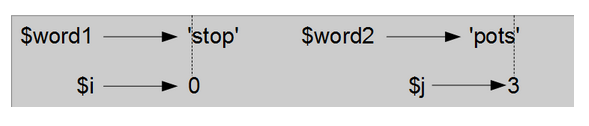
\includegraphics[scale=0.5]{figs/state6.png}}
\caption{State diagram.}
\label{fig.state4}
\end{figure}

We took some license by arranging the variables in the frame
and adding dotted lines to show that the values of {\tt \$i} 
and {\tt \$j} indicate characters in {\tt \$word1} and 
{\tt \$word2}.

Starting with this diagram, run the program on paper, changing 
the values of {\tt \$i} and {\tt \$j} during each iteration. 
Find and fix the second error in this function.

Solution: \ref{sol_isreverse}.
\label{isreverse}
\index{is-reverse}


\section{Glossary}

\begin{description}

\item[Object] Something a variable can refer to.  For now,
you can use ``object'' and ``value'' interchangeably.
\index{object}

\item[Sequence] An ordered collection of
values where each value is identified by an integer index.
\index{sequence}

\item[Item] One of the values in a sequence.
\index{item}

\item[Index] An integer value used to select an item in
a sequence, such as a character in a string.  In Perl
indices start from 0.
\index{index}

\item[Slice] A part of a string specified by a range of indices.
\index{slice}

\item[Empty string] A string with no characters and length 0, represented
by two quotation marks.
\index{empty string}

\item[Traverse] To iterate through the items in a sequence,
performing a similar operation on each.
\index{traversal}

\index{search}
\item[Search] A pattern of traversal that stops
when it finds what it is looking for.
\index{search!pattern}
\index{pattern!search}

\index{counter}
\item[Counter] A variable used to count something, usually initialized
to zero and then incremented.

\index{regular expression}
\item[Regular expressions] A computing sublanguage derived 
from the formal language theory.

\index{pattern}
\item[Pattern] A sequence of characters using a special 
syntax to describe from left to right the content that 
is intended to be matched within a target string.

\index{regex}
\item[Regexes] A pattern-matching sublanguage of Perl~6 
derived from regular expressions.

\index{backtracking}
\item[Backtracking] The process by which when a given attempt 
to match a string fails, the regex engine abandons part of 
the current match attempt, goes back into the string, and 
tries to see if it can find another route to a successful 
match. The backtracking process eventually stops as soon 
as a successful match succeeds, or ultimately when all 
possible match possibilities have failed.

\end{description}


\section{Exercises}


\begin{exercise}
\label{count_a}
\index{count method}
\index{method!count}
\index{index function}

Write a subroutine that uses the {\tt index} function in a 
loop to count the number of ``a'' characters in \verb"'banana'",
as we did in Section~\ref{counter}. Modify it to count 
any letter in any word passed as arguments to the subroutine.

Write another subroutine counting a given letter in a given 
word using the {\tt substr} function.
\index{substr function}

Solution: \ref{sol_count_a}
\end{exercise}


\begin{exercise}

\label{islower}
\index{lower case!character class}
\index{character class}
The \verb'<[a..z]>' character class matches any lower case 
character (only plain ASCII lower case characters, not 
Unicode characters). The following subroutine:

\begin{verbatim}[fontshape=up]
sub is-lower (Str $input) { 
    return so $char ~~ /^<[a..z]>$/
}
\end{verbatim}

should return {\tt True} if its argument is an ASCII lower case 
letter and {\tt False} otherwise. Test that it works as 
expected (and amend it if needed). The {\tt so} function 
coerces the result of the regex match into a Boolean value.

The following subroutines use the {\tt is-lower} subroutine 
and are all {\em intended} to check 
whether a string contains any lowercase letters, but at 
least some of them are wrong.  Analyze each subroutine by hand, 
determine whether it is correct, and describe what it 
actually does (assuming that the parameter is a string). Then 
test them with various input strings to check whether your 
analysis was correct.

\begin{verbatim}[fontshape=up]
# ATTENTION: some of the subroutines below are wrong

sub any_lowercase1(Str $string){
    for $string.comb -> $char {
        if is-lower $char {
            return True;
        } else {
            return False;
        }
    }
}

sub any_lowercase2(Str $string){
    for $string.comb -> $char {
        if is-lower "char" {
            return True;
        } else {
            return False;
        }
    }
}

sub any_lowercase3(Str $string){
    my $flag;
    for $string.comb -> $char {
        $flag =  is-lower $char;
    }
    return $flag;
}

sub any_lowercase4(Str $string){
    my $flag = False;
    for $string.comb -> $char {
        $flag = $flag or is-lower $char;
    }
    return $flag;
}

sub any_lowercase5(Str $string){
    my $flag = False;
    for $string.comb -> $char {
        if is-lower $char {
            $flag = True;
        }
    }
    return $flag;
}

sub any_lowercase6(Str $string){
    for $string.comb -> $char {
        if is-lower $char {
            return 'True';
        }
    }
    return 'False';
}

sub any_lowercase7(Str $string){
    for $string.comb -> $char {
        return True if is-lower $char;
    }
    return False;
}

sub any_lowercase8(Str $string){
    for $string.comb -> $char {
        return False unless is-lower $char;
    }
    return True;
}

sub any_lowercase9(Str $string){
    for $string.comb -> $char {
        if not is-lower $char {
            return False;
        }
    return True;
    }
}
\end{verbatim}

Solution: \ref{sol_islower}.

\end{exercise}


\begin{exercise}
\index{letter rotation}
\index{rotation, letter}
\index{Caesar cipher}

\label{rotate}
A Caesar cipher is a weak form of encryption that involves 
``rotating'' each letter by a fixed number of places.  To 
rotate a letter means to shift it through the alphabet, 
wrapping around to the beginning if necessary, so ``A'' 
rotated by 3 is ``D'' and ``Z'' rotated by 1 is ``A.''

To rotate a word, rotate each letter by the same amount.
For example, ``cheer'' rotated by 7 is ``jolly'' and ``melon'' rotated
by -10 is ``cubed.''  In the movie {\em 2001: A Space Odyssey}, the 
ship computer is called HAL, which is IBM rotated by -1.

Write a function called \verb"rotate-word"
that takes a string and an integer as parameters, and returns
a new string that contains the letters from the original string
rotated by the given amount.  

You might want to use the built-in functions {\tt ord}, which 
converts a character to a numeric code (Unicode code point), and 
{\tt chr}, which converts such numeric codes back to characters:
\index{ord function}
\index{chr function}
\index{function!ord}
\index{function!chr}

\begin{verbatim}[fontshape=up]
> say 'c'.ord;
99
> say chr 99
c
\end{verbatim}
%

Letters of the alphabet are encoded in alphabetical
order, so for example:
\index{alphabetic order}

\begin{verbatim}[fontshape=up]
> ord('c') - ord('a')
2
\end{verbatim}

because \verb"'c'" is the second letter after \verb"'a'" in 
the alphabet.  But beware: the numeric codes for upper case 
letters are different.
\index{upper case}
\index{case!upper}

\index{rot13}
Potentially offensive jokes on the internet are sometimes 
encoded in ROT13, which is a Caesar cipher with rotation 13. 
Since 13 is half the number of letters in our alphabet, 
applying rotation 13 twice returns the original word, 
so that the same procedure can be used for both encoding 
and decoding in rotation 13. If you are not
easily offended, find and decode some of these jokes.  

Solution: \ref{sol_rotate}.

\end{exercise}




\chapter{Case Study: Word Play}
\label{wordplay}

This chapter is intended to let you practice and 
consolidate the knowledge you have acquired so far, 
rather than introducing new concepts. To help you gain 
experience with programming, we will cover a 
case study that involves solving word puzzles by 
searching for words that have certain properties.  
For example, we'll find the longest palindromes
in English and search for words whose letters appear in
alphabetical order.  And I will present another program 
development plan: reduction to a previously solved problem.


\section{Reading from and Writing to Files}

For the exercises in this chapter, we will need our 
programs to read text from files. In many programming 
languages, this often means that we need a statement to 
open a file, then a statement or group of statements to 
read the file's content, and finally a statement to 
close the file (although this last operation may 
be performed automatically in some circumstances).
\index{file!reading from}
\index{file!writing to}
\index{file!open statement}
\index{file!close statement}

We are interested here in text files that are usually 
made of lines separated by logical new line characters; 
depending on your operating system, such logical new line 
characters consist of either one (Linux, Mac) or two (Windows) 
physical characters (bytes). 
\index{newline character}

The Perl built-in function {\tt open} takes the path and 
name of the file as a parameter and returns a {\bf file 
handle} ({\tt IO::Handle object}) which you can use to read 
the file (or to write to it):
\index{open function}
\index{function!open}
\index{plain text}
\index{text!plain}
\index{object!file}
\index{file handle}
\index{function!slurp-rest}

\begin{verbatim}
my $fh = open("path/to/myfile.txt", :r);
my $data = $fh.slurp-rest;
$fh.close;
\end{verbatim}
%
The {\tt :r} option is the file mode ({\tt read}). {\tt \$fh} is a 
common name for a file handle.  The \emph{file object} provides methods 
for reading, such as {\tt slurp-rest} which returns the 
full content of the file from the current position to the 
end (and the entire content of the file if we've just 
opened it).

This is the traditional way of opening and reading files 
in most languages.
\index{read mode}
\index{file mode!read}

However, Perl's {\tt IO} role (in simple terms, a role is 
a collection of related methods) offers simpler methods which 
can open a file and read it all in one single instruction (i.e., 
without having to first open a file handle and then close it):
\index{role}
\index{IO role}

\begin{verbatim}
my $text = slurp "path/to/myfile.txt";
# or:
my $text = "path/to/myfile.txt".IO.slurp;
\end{verbatim}
%

\index{slurp function}
{\tt slurp} takes care of opening and closing the file for you.

We can also read the file line by line, which is very 
practical if each line contains a logical entity such as 
a record, and is especially useful for very large files 
that might not fit into memory:

\begin{verbatim}
for 'path/to/hugefile.txt'.IO.lines -> $line {
    # Do something with $line
}
\end{verbatim}
%
By default, the {\tt .lines} method will remove the trailing 
newline characters from each line, so that you don't have 
to worry about them.
\index{IO.lines method}
\index{IO.slurp method}
\index{slurp function}
%

We haven't studied arrays yet, but you can also read all 
lines of a file into an array, with each line of the file 
becoming an array item. For example, you can load the 
\emph{myfile.txt} file into the \verb'@lines' array:
\index{array}

\begin{verbatim}
my @lines = "myfile.txt".IO.lines;
\end{verbatim}
%

Accessing any line can then be done with the bracket operator 
and an index. For example, to print the first and the 
seventh line:

\begin{verbatim}
say @lines[0];
say @lines[6];
\end{verbatim}
%
To write data to a file, it is possible to {\tt open} a file just 
as when wanting to read from it, except that the {\tt :w} (write) 
option should be used:
\index{write mode}
\index{file mode!write}

\begin{verbatim}
my $fh = open("path/to/myfile.txt", :w);
$fh.say("line to be written to the file");
$fh.close;
\end{verbatim}

Be careful with this. If the file already existed, any 
existing content will be clobbered. So watch out when 
you want to open a file in write mode.

It is also possible to open the file in append mode, using the 
{\tt :a} option. New data will then be added after the existing 
content.
\index{append mode}
\index{file mode!append}

Writing to a file can be simplified using the {\tt spurt} 
function, which opens the file, writes the data to it, 
and closes it:
\index{spurt function}

\begin{verbatim}
spurt "path/to/myfile.txt", "line to be written to the file\n";
\end{verbatim}

Used this way, {\tt spurt} will clobber any existing content in 
the file. It may also be used in append mode with the {\tt :append} 
option:
\index{spurt function!append mode}

\begin{verbatim}
spurt "path/to/myfile.txt", "line to be added\n", :append;
\end{verbatim}


\section{Reading Word Lists}
\label{wordlist}

For the exercises in this chapter we need a list of English 
words. There are lots of word lists available on the web, 
but one of the most suitable for our purpose is one of the 
word lists collected and contributed to the public domain 
by Grady Ward as part of the Moby lexicon project (see 
\url{http://wikipedia.org/wiki/Moby_Project}).  It is a 
list of 113,809 official crosswords; that is, words that are
considered valid in crossword puzzles and other word games.  
In the Moby collection, the filename is \emph{113809of.fic}; 
you can download a copy, with the simpler name \emph{words.txt}, 
from \url{https://github.com/LaurentRosenfeld/thinkperl6/tree/master/Supplementary/words.txt}.
\index{Moby Project}
\index{crosswords}
\index{word list}

This file is in plain text (with each word of the list on 
its own line), so you can open it with a text
editor, but you can also read it from Perl. Let's do so 
in the interactive mode (with the REPL):
\index{interactive mode}
\index{REPL}

\begin{verbatim}
> my $fh = open("words.txt", :r);
IO::Handle<words.txt>(opened, at octet 0)
> my $line = get $fh;
aa
> say "<<$line>>";
<<aa>>
\end{verbatim}

The {\tt get} function reads one line from the file handle. 
\index{get function}

The first word in this particular list is ``aa'' (a kind 
of lava).

Printing the \verb'$line' variable between angle brackets 
within a string shows us that the {\tt get} function removed 
implicitly the trailing newline characters, in this 
case a \verb'\r\n' (carriage return and newline) character 
combination, since this file was apparently prepared under 
Windows.

The file handle keeps track of what has been read from the 
file and what it should read next, so if you call {\tt get} 
again, you obtain the next line:

\begin{verbatim}
> my $line = get $fh;
aah
\end{verbatim}
%
The next word is ``aah,'' which is a perfectly legitimate
word, so stop looking at me like that.

This is good and fine if we want to explore the first few 
lines of the {\tt words.txt} file, but we are not going to 
read the 113 k-lines of the file this way.

We need a loop to do it for us. We could insert the above 
{\tt get} instruction into a {\tt while} loop, but we have 
seen above an easier and more efficient way of doing it 
using a {\tt for} loop and the {\tt IO.lines} method, 
without the hassle of having to open or close the file:
\index{for loop}
\index{IO.lines method}

\begin{verbatim}
for 'words.txt'.IO.lines -> $line {
    say $line;
}
\end{verbatim}
%
This code reads the file line by line, and prints each line 
to the screen. We'll soon do more interesting things than 
just displaying the lines on the screen.

\section{Exercises}

This case study consists mainly of exercises and 
solutions to them within the body of the chapter because solving the 
exercises is the main teaching material of this chapter. Therefore, 
solutions to these exercises are in the following sections of 
this chapter, not in the appendix. You should at least 
attempt each one before you read the solutions.

\begin{exercise}
Write a program that reads {\tt words.txt} and prints only the
words with more than 20 characters.
\index{whitespace}

\end{exercise}

\begin{exercise}

In 1939 Ernest Vincent Wright published a 50,000-word novel 
called {\em Gadsby} that does not contain the letter ``e''. 
Since ``e'' is the most common letter in English, that's 
not easy to do. In fact, it is difficult to construct a 
solitary thought without using that most common letter. 
Such a  writing in which one letter is avoided is sometimes 
called a lipogram.
\index{Wright, Ernest Vincent}
\index{Gadsby}
\index{lipogram}

Write a subroutine called \verb"has-no-e" that returns 
{\tt True} if the given word doesn't have the letter ``e'' 
in it.
\label{no_e}

Modify your program from the previous exercise to print only 
the words that have no ``e'' and compute the percentage of 
the words in the list that have no ``e''.

(The word dictionary we are using, \emph{words.txt}, is 
entirely in lower-case letters, so you don't need to 
worry about any uppercase ``E.'')



\end{exercise}


\begin{exercise} 

Write a subroutine named {\tt avoids}
that takes a word and a string of forbidden letters, and
that returns {\tt True} if the word doesn't use any of 
the forbidden letters.

Next, modify your program to prompt the user to enter a string
of forbidden letters and then print the number of words that
don't contain any of them.
Can you find a combination of five forbidden letters that
excludes the smallest number of words?

\end{exercise}



\begin{exercise}

Write a subroutine named \verb"uses-only" that takes a word and a
string of letters, and that returns {\tt True} if the word contains
only letters in the list.  Can you make a sentence using only the
letters {\tt acefhlo}?  Other than ``Hoe alfalfa?''

\end{exercise}


\begin{exercise} 

Write a subroutine named \verb"uses-all" that takes a word and a
string of required letters, and returns {\tt True} if the word
uses all the required letters at least once.  How many words are there
that use all the vowels {\tt aeiou}?  How about {\tt aeiouy}?

\end{exercise}


\begin{exercise}

Write a function called \verb"is_abecedarian" that returns
{\tt True} if the letters in a word appear in alphabetical order
(double letters are ok).  
How many abecedarian words are there?

\index{abecedarian}

\end{exercise}



\section{Search}
\label{search}
\index{search!pattern}
\index{pattern!search}
\index{regex}

Most of the exercises in the previous section have something
in common; they can be solved with the search pattern (and 
the {\tt index} function we saw in Section~\ref{find} 
(p.~\pageref{find}). Most can also be solved using regexes.

\subsection{Words Longer Than 20 Characters (Solution)}

The solution to the simplest exercise ---printing all the 
words of {\tt words.txt} that are longer than 
20~characters--- is:

\begin{verbatim}
for 'words.txt'.IO.lines -> $line {
    say $line if $line.chars > 20
}
\end{verbatim}
%

Because the code is so simple, this is a typical example 
of a possible and useful one-liner (as described in 
Section~\ref{one-liner mode}). Assuming you want to know the words 
that are longer than 20~characters, you don't even need to 
write a script, save it, and run it. You can simply type this at 
your operating system prompt:
\label{one-liner-example}
\index{one-liner mode}

\begin{verbatim}
$ perl6 -n -e '$_.say if $_.chars > 20;' words.txt
\end{verbatim} 
%
The ``-e'' option tells Perl that the script to be run 
comes next on the command line between quotation marks. The 
``-n'' asks Perl to read line by line the file after the 
end of the command line, to store each line in the \verb'$_' 
topical variable, and to apply the content of the script to 
each line. And the one-liner script is just printing the 
content of \verb'$_' if its length is greater than 20.
\index{topical variable}

To simplify a bit, the two options \verb'-n' and \verb'-e' 
may be grouped together as \verb"perl6 -ne". In addition, 
the \verb'$_' topical variable can be omitted in method calls 
(in other words, if a method has no invocant, the invocant 
will be defaulted to \verb'$_'). Finally, the trailing 
semi-colon may also be removed. The one-liner above can 
thus be made somewhat simpler and shorter:
\index{invocant}

\begin{verbatim}
$ perl6 -ne '.say if .chars > 20' words.txt
\end{verbatim} 
%
Remember that, if you're trying this under Windows, you need to 
replace the single quotes with double quotes (and vice-versa if 
the scripts itself contains double quotes):

\begin{verbatim}
C:\Users\Laurent>perl6 -ne ".say if .chars > 20" words.txt
\end{verbatim} 
%

\subsection{Words with No ``e'' (Solution)}

A subroutine that returns {\tt True} for words that have 
no ``e'' (Exercise~\ref{no_e}) is also quite straight forward:

\begin{verbatim}
sub has-no-e (Str $word) {
    return True unless defined index $word, "e";
    return False;
}
\end{verbatim}
%

The subroutine simply returns {\tt True} if the {\tt index} 
function did not find any ``e'' in the word received as 
a parameter and {\tt False} otherwise. 

Note that this works correctly because the word list used 
\emph{words.txt}) is entirely in lowercase letters. The 
above subroutine would need to be modified if it might 
be called with words containing uppercase letters. 

Since the {\tt defined} function returns a Boolean value, we 
could shorten our subroutine to this:
\begin{verbatim}
sub has-no-e (Str $word) {
    not defined index $word, "e";
}
\end{verbatim}
%

We could also have used a regex for testing the presence of a 
``e'' on the second line of this subroutine:

\begin{verbatim}
    return True unless $word ~~ /e/;
\end{verbatim}
%

This fairly concise syntax is appealing, but when 
looking for an exact literal match, the {\tt index} function 
is likely to be slightly more efficient (faster) than a 
regex.

Looking for the words without ``e'' in our word list and 
counting them is not very difficult:

\begin{verbatim}
sub has-no-e (Str $word) {
    not defined index $word, "e";
}

my $total-count = 0;
my $count-no-e = 0;
for 'words.txt'.IO.lines -> $line { 
    $total-count++;
    if has-no-e $line {
        $count-no-e++;
        say $line;
    }
}
say "=" x 24;
say "Total word count: $total-count";
say "Words without 'e': $count-no-e";
printf "Percentage of words without 'e': %.2f %%\n", 
        100 * $count-no-e / $total-count;
\end{verbatim}

The above program will display the following at the end 
of its output:

\begin{verbatim}
========================
Total word count: 113809
Words without 'e': 37641
Percentage of words without 'e': 33.07 %
\end{verbatim}

So, less than one third of the words of 
our list have no ``e.''

\subsection{Avoiding Other Letters (Solution)}

\index{generalization}
The {\tt avoids} subroutine is a more general version of 
\verb"has_no_e", but it has the same structure:

\begin{verbatim}
sub avoids (Str $word, Str $forbidden) {
    for 0..$forbidden.chars - 1 -> $idx {
        my $letter = substr $forbidden, $idx, 1;
        return False if defined index $word, $letter;
    }
    True;
}
\end{verbatim}
%
We can return {\tt False} as soon as we find a forbidden letter;
if we get to the end of the loop, we return {\tt True}. Since 
a subroutine returns the last evaluated expression, we don't 
need to explicitly use a {\tt return True} statement in the last 
code line above. I used this feature here as an example; you might 
find it clearer to explicitly {\tt return} values, except 
perhaps for very simple one-line subroutines.

Note that we have here implicitly two nested loops. We could 
reverse the outer and the inner loops:

\begin{verbatim}
sub avoids (Str $word, Str $forbidden) {
    for 0..$word.chars - 1 -> $idx {
        my $letter = substr $word, $idx, 1;
        return False if defined index $forbidden, $letter;
    }
    True;
}
\end{verbatim}
%

The main code calling the above subroutine is similar to 
the code calling {\tt has-no-e} and might look like 
this:

\begin{verbatim}
my $total-count = 0;
my $count-no-forbidden = 0;

for 'words.txt'.IO.lines -> $line { 
    $total-count++;
    $count-no-forbidden++ if avoids $line, "eiou";
}

say "=" x 24;
say "Total word count: $total-count";
say "Words without forbidden: $count-no-forbidden";
printf "Percentage of words with no forbidden letter: %.2f %%\n", 
        100 * $count-no-forbidden / $total-count;
\end{verbatim}    
%
  

\subsection{Using Only Some Letters (Solution)}

\verb"uses-only" is similar to our {\tt avoids} subroutine 
except that the sense of the condition is reversed:

\begin{verbatim}
sub uses-only (Str $word, Str $available) {
    for 0..$word.chars - 1 -> $idx {
        my $letter = substr $word, $idx, 1;
        return False unless defined index $available, $letter;
    }
    True;
}
\end{verbatim}
%
Instead of a list of forbidden letters, we have a list 
of available letters.  If we find a letter in {\tt \$word} that 
is not in {\tt \$available}, we can return {\tt False}. And 
we return {\tt True} if we reach the loop end.

\subsection{Using All Letters of a List (Solution)}

\verb"uses-all" is similar to the previous two subroutines, 
except that we reverse the role of the word and the string 
of letters:

\begin{verbatim}
sub uses-all(Str $word, Str $required) {
    for 0..$required.chars - 1 -> $idx {
        my $letter = substr $word, $idx, 1;
        return False unless defined index $word, $letter;
    }
    return True;
}
\end{verbatim}
%
Instead of traversing the letters in {\tt \$word}, the loop
traverses the required letters.  If any of the required letters
do not appear in the word, we can return {\tt False}.
\index{traversal}

If you were really thinking like a computer scientist, you would
have recognized that \verb"uses-all" was an instance of a
previously solved problem in reverse: if word~A uses all 
letters of word~B, then word~B uses only letters of word~A. So, 
we can call the {\tt uses-only} subroutine and write:

\begin{verbatim}
sub uses-all ($word, $required) {
    return uses-only $required, $word;
}
\end{verbatim}
%
This is an example of a program development plan called 
{\bf reduction to a previously solved problem}, which means that you
recognize the problem you are working on as an instance of a solved
problem and apply an existing solution. 
\index{reduction to a previously solved problem} 
\index{development plan!reduction}

\subsection{Alphabetic Order (Solution)}

For \verb"is_abecedarian" we have to compare adjacent letters. 
Each time in our {\tt for} loop, we define one letter as our 
current letter and compare it with the previous one:

\begin{verbatim}
sub is_abecedarian ($word) {
    for 1..$word.chars - 1 -> $idx {    
        my $curr-letter = substr $word, $idx, 1;
        return False if $curr-letter lt substr $word, $idx - 1, 1;  
    }     
    return True
}
\end{verbatim}

An alternative is to use recursion:
\index{recursion}

\begin{verbatim}
sub is-abecedarian (Str $word) {
    return True if $word.chars <= 1;
    return False if substr($word, 0, 1) gt substr($word, 1, 1);
    return is-abecedarian substr $word, 1;
}
\end{verbatim}

Another option is to use a {\tt while} loop:

\begin{verbatim}
sub is_abecedarian (Str $word):
    my $i = 0;
    while $i < $word.chars -1 {
        if substr($word, $i, 1) gt substr ($word, $i+1, 1) {
            return False;
        }
        $i++;
    }
    return True;
}
\end{verbatim}
%
The loop starts at {\tt \$i=0} and ends when {\tt i=\$word.chars -1}.  Each
time through the loop, it compares the $i$th character (which you can
think of as the current character) to the $i+1$th character (which you
can think of as the next).

If the next character is less than (alphabetically before) the current
one, then we have discovered a break in the abecedarian trend, and
we return {\tt False}.

If we get to the end of the loop without finding a fault, then the
word passes the test.  To convince yourself that the loop ends
correctly, consider an example like \verb"'flossy'".  The
length of the word is 6, so
the last time the loop runs is when \verb'$i' is 4, which is the
index of the second-to-last character.  On the last iteration,
it compares the second-to-last character (the second ``s'') to 
the last (the ``y''), which is what we want.

\subsection{Another Example of Reduction to a Previously Solved Problem}

\index{palindrome}
\label{palindrome_2}
Here is a version of \verb"is_palindrome" (see
Exercise~\ref{palindrome}) that uses two indices; one starts at the
beginning and goes up, while the other starts at the end and goes down:		

\begin{verbatim}
sub one-char (Str $string, $idx) {
    return substr $string, $idx, 1;
}
sub is-palindrome (Str $word) {
    my $i = 0;
    my $j = $word.chars - 1;

    while $i < $j {
        return False if one-char($word, $i) ne one-char($word, $j);
        $i++;
        $j--;
    }
    return True;
}
\end{verbatim}

Or we could reduce to a previously solved
problem and write:
\index{reduction to a previously solved problem}
\index{development plan!reduction}

\begin{verbatim}
sub is-palindrome (Str $word) {
    return is-reverse($word, $word)
}
\end{verbatim}
%
using \verb"is-reverse" from Section~\ref{isreverse} (but
you should probably choose the corrected version of the 
{\tt is-reversed} subroutine given in the appendix: 
see Subsection~\ref{sol_isreverse}).


\section{Debugging}
\index{debugging}
\index{testing!is hard}
\index{program!testing}

Testing programs is hard.  The functions in this chapter are
relatively easy to test because you can check the results by hand.
Even so, it is somewhere between difficult and impossible to choose a
set of words that test for all possible errors.

Taking \verb"has_no_e" as an example, there are two obvious
cases to check: words that have an ``e'' should return {\tt False}, and
words that don't should return {\tt True}.  You should have no
trouble coming up with one of each.

Within each case, there are some less obvious subcases.  Among the
words that have an ``e'', you should test words with an ``e'' at the
beginning, the end, and somewhere in the middle.  You should test long
words, short words, and very short words, like an empty string.  The
empty string is an example of a {\bf special case}, which is one of
the nonobvious cases where errors often lurk.
\index{special case}

In addition to the test cases you generate, you can also test
your program with a word list like \emph{words.txt}.  By scanning
the output, you might be able to catch errors, but be careful:
you might catch one kind of error (words that should not be
included, but are) and not another (words that should be included,
but aren't).

In general, testing can help you find bugs, but it is not easy to
generate a good set of test cases, and even if you do, you can't
be sure your program is correct.

According to a legendary computer scientist:
\index{testing!and absence of bugs}

\begin{quote}
Program testing can be used to show the presence of bugs, 
but never to show their absence!

--- Edsger W. Dijkstra
\end{quote}
\index{Dijkstra, Edsger}


\section{Glossary}

\begin{description}

\item[File object] A value that represents an open file.
\index{file object}
\index{object!file}

\item[Reduction to a previously solved problem] A way of solving a
  problem by expressing it as an instance of a previously solved
  problem.
  \index{reduction to a previously solved problem}
  \index{development plan!reduction}

\item[Special case] A test case that is atypical or nonobvious
(and less likely to be handled correctly). The expressions   
\emph{edge case} and \emph{corner case} convey more or less 
the same idea.
\index{special case}
\index{edge case}
\index{corner case}

\end{description}


\section{Exercises}

\begin{exercise}
\index{Car Talk}
\index{Puzzler}
\index{double letters}
\label{cartalk}

This question is based on a Puzzler that was broadcast on the radio
program {\em Car Talk} 
(\url{http://www.cartalk.com/content/puzzlers}):

\begin{quote}
Give me a word with three consecutive double letters. I'll give you a
couple of words that almost qualify, but don't. For example, the word
committee, c-o-m-m-i-t-t-e-e. It would be great except for the ``i'' that
sneaks in there. Or Mississippi: M-i-s-s-i-s-s-i-p-p-i. If you could
take out those i's it would work. But there is a word that has three
consecutive pairs of letters and to the best of my knowledge this may
be the only word. Of course there are probably 500 more but I can only
think of one. What is the word?
\end{quote}

Write a program to find it.

Solution: \ref{sol_cartalk}.

\end{exercise}


\begin{exercise}
Here's another {\em Car Talk}
Puzzler (\url{http://www.cartalk.com/content/puzzlers}):
\label{cartalk2}
\index{Car Talk}
\index{Puzzler}
\index{odometer}
\index{palindrome}

\begin{quote}
``I was driving on the highway the other day and I happened to
notice my odometer. Like most odometers, it shows six digits,
in whole miles only. So, if my car had 300,000
miles, for example, I'd see 3-0-0-0-0-0.

``Now, what I saw that day was very interesting. I noticed that the
last 4 digits were palindromic; that is, they read the same forward as
backward. For example, 5-4-4-5 is a palindrome, so my odometer
could have read 3-1-5-4-4-5.

``One mile later, the last 5 numbers were palindromic. For example, it
could have read 3-6-5-4-5-6.  One mile after that, the middle 4 out of
6 numbers were palindromic.  And you ready for this? One mile later,
all 6 were palindromic!

``The question is, what was on the odometer when I first looked?''
\end{quote}

Write a program that tests all the six-digit numbers and prints
any numbers that satisfy these requirements.
  
Solution: \ref{sol_cartalk2}.

\end{exercise}


\begin{exercise}
Here's another {\em Car Talk} Puzzler you can solve with a
search (\url{http://www.cartalk.com/content/puzzlers}):
\index{Car Talk}
\index{Puzzler}
\index{palindrome}
\label{cartalk3}

\begin{quote}
Recently I had a visit with my mom and we realized that
the two digits that make up my age when reversed resulted in her
age. For example, if she's 73, I'm 37. We wondered how often this has
happened over the years but we got sidetracked with other topics and
we never came up with an answer.

When I got home I figured out that the digits of our ages have been
reversible six times so far. I also figured out that if we're lucky it
would happen again in a few years, and if we're really lucky it would
happen one more time after that. In other words, it would have
happened 8 times over all. So the question is, how old am I now?

\end{quote}

Write a Perl program that searches for solutions to this Puzzler.
Hint: you might find the string formatting method 
{\tt sprintf} useful.
\index{sprintf function}

Solution: \ref{sol_cartalk3}.

\end{exercise}





\chapter{Arrays and Lists}
\label{arrays}

This chapter presents some of Perl's most useful built-in types, 
arrays and lists.


\section{Lists and Arrays Are Sequences}
\label{sequence}

Like strings, {\bf lists} and {\bf arrays} are sequences of 
values.  In a string, the values are characters; in a list or
in an array, they can be any type.  The values in a list or 
in an array are called {\bf elements} or sometimes {\bf items}.
\index{list}
\index{array}
\index{type!list}
\index{type!array}
\index{element}
\index{sequence}
\index{item}

There are several important differences between lists and arrays. The main ones 
are that lists are ordered and immutable collections of items: 
you can't change the number of items in a list and you can't 
change the individual items either. Arrays, by contrast, are 
variables and are generally mutable: you can add elements 
to an array, or remove elements from it. And you can access 
the individual elements of an array and modify them. For this 
to be possible, arrays usually have a name (as do other variables), 
although some arrays are anonymous, which means that they 
have no name, but have some other ways of accessing them.

A list is also ephemeral (unless it is assigned 
to a variable or some other thing): it ceases to exist as 
soon as it has been used, usually as soon as the program 
control flow goes to the next code line. An array, on the 
other hand, has some form of persistence: you may be able to 
use it somewhere else in the program if the variable 
containing it is still within scope.

There are several ways to create a new list; the simplest is 
to enumerate its values, separated by commas:
\index{comma operator}
\index{operator!comma}

\begin{verbatim}
> 3, 4, 5
(3 4 5)
> say (3, 4, 5).WHAT;
(List)
say $_ for 1, 2, 3;
1
2
3
\end{verbatim}
%

You don't need parentheses to create a list, but they are 
often useful to delimit it, i.e., to stipulate where 
it starts and where it ends, and, in some cases, to override 
precedence.

We used lists earlier in this book. If we write:

\begin{verbatim}
> print "$_ " for 1, 3, 5, 9, "\n";
1 3 5 9
 >
> print "$_ " for 1..10;
1 2 3 4 5 6 7 8 9 10 >
\end{verbatim}

we are basically creating and using a list of integers (from 
the standpoint of the type hierarchy of Perl; this observation is 
not entirely accurate technically for the second example, since 
\verb'1..10' has a \emph{Range} type, and it gets 
transformed into a \emph{Seq} type, but this approximation is 
good enough for our purposes here).
\index{range!type}
\index{range!operator}

Arrays are variables whose names start with the sigil \verb'@'.
Named arrays  need to be declared before they are used, just 
as any other variable we've seen so far (except the topical 
variable, \verb'$_'). One of the easiest 
ways to create an array is to assign a list to it:
\index{topical variable}
\index{sigil}

\begin{verbatim}
> my @odd_digits = 1, 3, 5, 7, 9;
[1 3 5 7 9]
> say @odd_digits.WHAT;
(Array)
> my @single_digit_numbers = 0..9;
[0 1 2 3 4 5 6 7 8 9]
\end{verbatim}

Under the Perl REPL, an array is displayed between square 
brackets (\verb"[" and \verb"]"), while lists are displayed 
between round parentheses.
\index{REPL}
\index{square bracket operator}
\index{operator!square bracket}
\index{bracket!square}

If the items don't contain any space characters, it is quite handy 
to construct a list (and assign it to an array if needed) using 
the \verb'<...>' quote-word operator:
\index{quote-word operator}

\begin{verbatim}
> my @weekdays = <mon tue wed thu fri>;
[mon tue wed thu fri]
> my @weekend = <sat sun>;
[sat sun]
\end{verbatim}

The advantage of this construction is that there is no need to 
separate the items with commas and no need to insert them between 
quotes when the items are strings. Basically, 
the quote-word operator breaks up its content on whitespace 
and returns a list of words, which can then be 
used in a loop or assigned to an array as in the example 
above.

Most of the rest of this chapter will be devoted to arrays 
rather than lists, but keep in mind that many of the array 
functions and operators we will study here also work on lists 
(at least most of those that would not violate the 
immutability property of lists).
 
The items of an array (or a list) don't need to be of the 
same type:

\begin{verbatim}
> my @heterogeneous-array = 1, 2.3, pi, "str", (1, 2, 4);
[1 2.3 3.14159265358979 str (1 2 4)]
\end{verbatim}

Here, the array is composed of an integer, a rational, a 
float ({\tt Num} type), a string, and a list of three integers. 
It may not be advisable for the sake of the developer's 
mental sanity to use an array with such wildly heterogeneous 
items, but Perl will not complain about that: it is up 
to you to make sense of your data.

The array above even contains a list of items. If you iterate 
over the elements of this array for example with a {\tt for} 
loop statement, this list will arrive as one distinct element; 
it will not get ``flattened'' as three elements 
of the array. Similarly, {\tt elems} is a method to 
count the number of items of an array (or of a list). 
Using it on the above array produces the following result:

\begin{verbatim}
> say @heterogeneous-array.elems;
5
\end{verbatim}
%

As you can see, the \verb'(1, 2, 4)' list ``counts'' 
as one single array element.

A list within another list is {\bf nested}.
\index{nested list}
\index{list!nested}

An array that contains no elements is
called an empty array; you can create one with empty
parentheses, \verb"()":
\begin{verbatim}
> my @empty = ();
[]
\end{verbatim}
\index{empty list}
\index{list!empty}

This code is really assigning an empty list to the array. But 
this syntax is usually not needed when creating a new empty array, 
since just declaring an array without defining it has the same 
effect:

\begin{verbatim}
> my @empty;
[]
\end{verbatim}

So using the empty parentheses (i.e., assigning an empty list) 
would be needed essentially for resetting an existing array to 
an empty array.


\section{Arrays Are Mutable}
\label{mutable}
\index{list!element}
\index{access}
\index{index}
\index{subscript}
\index{bracket operator}
\index{operator!bracket}
\index{bracket!square}

\index{index!starting at zero}
\index{coercion}
The syntax for accessing the elements of an array or a list 
uses the square brackets operator.  The expression inside the 
brackets specifies the index or subscript, which can be a 
literal integer (or some value that can be coerced into 
an integer), a variable containing a numerical value, a list 
or a range of numerical values, an expression or a piece 
of code returning a numerical value, etc.  Indices are offsets 
compared to the beginning of the array 
or the list (much in the same way as the values returned 
by the {\tt index} function on strings), so that they start 
at 0. Thus, the first item of an array has the index 0, the 
second item the index 1, and so on:
\index{zero, index starting at}


\begin{verbatim}
say <sat sun>[1];             # -> sun  (accessing a list item)
my @weekdays = <mon tue wed thu fri>;     # assigning an array
say "The third day is @weekdays[2]";      # -> The third day is wed
\end{verbatim}
%

You may also use ranges or lists of indices to access 
\emph{slices} of an array or a list:
\index{slice}
\index{slice!operator}
\index{operator!slice}
\index{index!slice}
\index{list!slice}
\index{slice!list}
\index{range}

\begin{verbatim}
> my @even-digits = 0, 2, 4, 6, 8;
[0 2 4 6 8]
> my @small-even_digits = @even-digits[0..2];
[0 2 4]
> my @min-max-even-digits = @even-digits[0, 4]
[0 8]
\end{verbatim}

If you need a slice in the opposite order, you can use the 
{\tt reverse} function to reverse the range:

\begin{verbatim}
> my @reverse-small-even_digits = @even-digits[reverse 0..2];
[4 2 0]
\end{verbatim}

or reverse the data returned by the slice expression:

\begin{verbatim}
> my @reverse-small-even_digits = reverse @even-digits[0..2];
[4 2 0]
\end{verbatim}

Unlike lists, arrays are mutable.  When the bracket operator 
appears after an array on the left side of an assignment, 
it identifies the element of the array that will be assigned:
\index{mutability}

\begin{verbatim}
> my @even-digits = 0, 2, 2, 6, 8;   # Oops, error on the second 2
[0 2 2 6 8]
> @even-digits[2] = 4; # fixing the faulty third digit
4
> say @even-digits
[0 2 4 6 8]
\end{verbatim}
%

The third element of {\tt \@even-digits}, which was  
(presumably by mistake) 2, is now 4. If the index corresponds 
to an item which does not exist yet in the array, the array 
will be expanded to include the new element:

\begin{verbatim}
> my @odds = 1, 3, 5;
[1 3 5]
> @odds[3] = 7;
7
> say @odds;
[1 3 5 7]
\end{verbatim}

\index{index!starting at zero}
\index{item assignment}
\index{assignment!item}
\index{reassignment}

\index{elems function or method}
\index{end method}
The {\tt elems} function or method returns the number of 
elements of an array. The {\tt end} function or method 
returns the index of the last element of an array:

\begin{verbatim}
my @nums = 1..5;      # -> [1 2 3 4 5]
say @nums.elems;      # -> 5
say elems @nums;      # -> 5
say @nums.end;        # -> 4
\end{verbatim}

The {\tt end} method returns the result of the {\tt elems} 
method minus one because, since indices start at 0, the 
index of the last element is one less than the number 
of elements.
\index{zero, index starting at}

The {\tt unique} function or method returns a sequence 
of unique elements of the input list or array (i.e., 
it returns the original list without any duplicate 
values):
\index{unique function}
\index{function!unique}

\begin{verbatim}
> say < a b d c a f d g>.unique;
(a b d c f g)
\end{verbatim}

If you know that the input is sorted (and that, therefore, 
duplicates are adjacent), use the {\tt squish} function 
instead of {\tt unique}, as this is likely to be more 
efficient. The {\tt squish} function removes adjacent 
duplicates.
\index{squish function}
\index{function!squish}

To know whether two arrays are identical (structurally the 
same, with the same type and same values), use the {\tt eqv} equivalence 
operator. To know whether they just contain the same elements, use 
the \verb'~~' smart match operator. Between two arrays or lists, the 
\verb'==' numeric equality operator will return {\tt True} if the 
arrays have the same number of elements and {\tt False} otherwise, 
because \verb'==' coerces its arguments to numeric type, so that 
it compares the number of elements:
\index{eqv operator}
\index{coercion}
\index{equivalence operator}
\index{operator!eqv}
\index{smart match operator}
\index{operator!smart match}
\index{numeric equality operator}
\index{operator!numeric equality}

\begin{verbatim}
> my @even1 = 0, 2, 4, 6, 8;
[0 2 4 6 8]
> my @even2 = reverse 8, 6, 4, 2, 0;
[0 2 4 6 8]
> say @even1 eqv @even2;          # same items, structurally the same
True
> say <1 2 3 4 5> eqv 1..5;       # same items, structurally different
False
> say <1 2 3 4 5> ~~ 1..5;        # same items, True
True
> my @array = 1..5;               
[1 2 3 4 5]
>  say <1 2 3 4 5> ~~ @array;     # same elements, True
True
>  say <1 2 3 4 6> ~~ @array;     # not the same elements
False
> say <1 2 3 4 5> == <5 6 7 8 9>; # compares the numbers of items
True
\end{verbatim}

The \verb'<1 2 3 4 5> eqv 1..5' statement returns \verb'False' because, 
although they have the same items, the arguments are structurally 
different entities (one is a list and the other one a range).

\section{Adding New Elements to an Array or Removing Some}

We've just seen that assigning an item to an index that does 
not exists yet will expand the array. There are other 
ways of expanding an array.

Perl has operators to add elements to, or remove one element 
from, an array:
\index{pop function}
\index{push function}
\index{shift function}
\index{unshift function}

\begin{itemize}
\item {\tt shift}: removes the first item of an array and returns it;
\item {\tt pop}: removes the last item of an array and returns it;
\item {\tt unshift}: adds an item or a list of items to the 
beginning of an array;
\item {\tt push}: adds an item or a list of items to the 
end of an array;
\end{itemize}

These are a few examples for each:

\begin{verbatim}
> my @numbers = <2 4 6 7>;
[2 4 6 7]
> push @numbers, 8, 9;
[2 4 6 7 8 9]
> unshift @numbers, 0, 1;
[0 1 2 4 6 7 8 9]
> my $num = shift @numbers
0
> $num = pop @numbers
9
> say @numbers
[1 2 4 6 7 8]
\end{verbatim}

As you might expect by now, these routines also come with a 
method invocation syntax. For example:
\index{invocation!method}
\index{method invocation}

\begin{verbatim}
> my @numbers = <2 4 6 7>;
[2 4 6 7]
> @numbers.push(8, 9)
[2 4 6 7 8 9]
\end{verbatim}

Note, however, that if you {\tt push} or {\tt unshift} an 
array onto another array, you'll get something different 
than what you might expect:

\begin{verbatim}
> my @numbers = <2 4 6 7>;
[2 4 6 7]
> my @add-array = 8, 10;
[8 10]
> @numbers.push(@add-array);
[2 4 6 7 [8 10]]
\end{verbatim}

As you can see, when \verb'@add-array' is added as an entity 
to the \verb'@numbers' array, \verb'@add-array' becomes 
the new last item of the original array. If you want to 
add the items of \verb'@add-array' to the original array, 
you may use the {\tt append} method instead of {\tt push}:

\begin{verbatim}
> my @numbers = <2 4 6 7>;
[2 4 6 7]
> @numbers.append(@add-array);
[2 4 6 7 8 10]
\end{verbatim}

Or you can use the ``|'' prefix operator to flatten the 
added array into a list of arguments:

\begin{verbatim}
> my @numbers = <2 4 6 7>;
[2 4 6 7]
> @numbers.push(|@add-array);
[2 4 6 7 8 10]
\end{verbatim}

There is also a {\tt prepend} method that can replace 
{\tt unshift} to add individual items of an array at the 
beginning of an existing array (instead of adding the array 
as a single entity).


\section{Stacks and Queues}
\label{stacks_queues}

\index{stack}
\index{queue}
Stacks and queues are very commonly used data structures in 
computer science.

\index{LIFO (last in / first out)}
\index{last in / first out (LIFO)}
A stack is a \emph{last in / first out (LIFO)} data structure. Think of 
piled-up plates. When you put a clean plate onto the stack, 
you usually put it on top; when you take out one, you also 
take it from the top. So the first plate that you take 
is the last one that you added. A CS stack implements the same 
idea: you use it when the first piece of data you need from a 
data structure is the last one you added.

\index{FIFO (first in / first out)}
\index{first in / first out (FIFO)}
A queue, by contrast, is a \emph{first in / first out (FIFO)} data 
structure. This is the idea of people standing in a 
line waiting to pay at the supermarket. The first 
person that will be served is the first person who entered 
the queue.

A stack may be implemented with an array and the {\tt push} 
and {\tt pop} functions, which respectively add an item (or 
several) at the end of an array and take one from the end of 
the array. This is a somewhat simplistic implementation of 
a stack:
\index{pop function}
\index{push function}   
\index{function!pop}
\index{function!push}
\label{stack_code}

\begin{verbatim}
sub put-in-stack (@stack, $new_item) {
    push @stack, $new_item;
}
sub take-from-stack (@stack) {
    my $item = pop @stack;
    return $item;
}
my @a-stack = 1, 2, 3, 4, 5;
put-in-stack @a-stack, 6;
say @a-stack;
say take-from-stack @a-stack for 1..3;
\end{verbatim}

This example will print this:

\begin{verbatim}
[1 2 3 4 5 6]
6
5
4
\end{verbatim}

\index{stack}
This stack is simplistic because, at the very least, a more 
robust implementation should do something sensible when you 
try to {\tt take-from-stack} from an empty stack. It would 
also be wise to add signatures to the subroutines. In 
addition, you might want to {\tt put-in-stack} more than 
one element in one go. Take a look at the solution to the 
exercise on queues below (Subsection~\ref{sol_exercise_queue}) 
to figure out on how this stack may be improved.
\index{signature}
\index{subroutine signature}

You could obtain the same stack features using the  
{\tt unshift} and {\tt shift} functions instead of {\tt push} 
and {\tt pop}. The items will be added at the beginning of 
the array and taken from the beginning, but you will still 
have the LIFO behavior.
\index{shift function}
\index{unshift function}
\index{push function}
\index{LIFO}

\label{exercise_queue}
As an exercise, try to implement a FIFO queue on the same model. 
Hint: you probably want to use an array and the {\tt unshift} 
and {\tt pop} functions (or the {\tt push} and {\tt shift} functions). Solution: \ref{sol_exercise_queue}.
\index{queue}
\index{shift function}
\index{unshift function}
\index{push function}
\index{pop function}
\index{FIFO}

\section{Other Ways to Modify an Array}
\label{modify_array}

The {\tt shift} and {\tt pop} functions remove respectively 
the first and the last item of an array and return that 
item. It is possible to do almost the same operation on any item 
of an array, using the {\tt delete} \emph{adverb}:

\begin{verbatim}
my @fruit = <apple banana pear cherry pineapple orange>;
my $removed = @fruit[2]:delete; 
say $removed;  # -> pear
say @fruit;    # -> [apple banana (Any) cherry pineapple orange]
\end{verbatim}

Notice that the third element (``pear'') is removed and 
returned, but the array is not reorganized; the operation leaves 
a sort of ``empty slot'', an undefined item, in the 
middle of the array. The colon (``:'') syntax used here is the 
operator for an adverb (we discussed adverbs in  
Section~\ref{regex} about regexes); 
for the time being, you may think of it as a kind of special 
method operating on one element of an item collection.

We have seen how to use array slices to retrieve several 
items of an array or a list at a time. The same slice syntax 
can also be used on the left side of an assignment to modify 
some elements of an array:
\index{slice!assignment}

\begin{verbatim}
my @digits = <1 2 3 6 5 4 7 8 9>
@digits[2..4] = 4, 5, 6
say @digits;   # -> [1 2 4 5 6 4 7 8 9]
\end{verbatim}

Of course, you can't do this with lists, since, as you 
remember, they are immutable.

The {\tt splice} function may be regarded as the Swiss Army 
knife of arrays. It can add, remove, and return one or 
several items to or from an array. The general syntax is 
as follows:

\begin{verbatim}
my @out_array = splice @array, $start, $num_elems, @replacement;
\end{verbatim}
%
The arguments for {\tt splice} are the input array, the index 
of the first element on which to make changes, the number of 
elements to be affected by the operation, and a list of 
replacements for the elements to be removed\footnote{Notice that 
the {\tt splice} function on arrays has almost the same syntax 
as the {\tt substr} function on strings. This may make it easier 
to understand them and remember their syntax.}. For example, 
to perform the slice assignment shown just above, it is 
possible to do this:

\begin{verbatim}
my @digits = <1 2 3 6 5 4 7 8 9>
my @removed_digits = splice @digits, 3, 3, 4, 5, 6;
say @removed_digits;     # -> [6 5 4]
say @digits;             # -> [1 2 3 4 5 6 7 8 9]
\end{verbatim}
%
Here, the {\tt splice} statement removed three elements (6, 5, 4) 
and replaced them with the replacement arguments (4, 5, 6). 
It also returned the removed items into \verb'@removed_digits'. 
The number of replacements does not need to be the same as the number 
of removed items, in which case the array size will grow or 
shrink. For example, if no replacement is provided, then 
{\tt splice} will just remove and return the required number 
of elements and the array size will be reduced by the same number:

\begin{verbatim}
my @digits = 1..9;
my @removed_digits = splice @digits, 3, 2;
say @removed_digits;     # -> [4 5]
say @digits;             # -> [1 2 3 6 7 8 9]
\end{verbatim}
%

Conversely, if the number of elements to be removed is zero, 
no element will be removed, an empty array will be returned, 
and the elements in the replacement list will be added in 
the right place:

\begin{verbatim}
my @digits = <1 2 3 6 4 7 8 9>;
my @removed_digits = splice @digits, 3, 0, 42;
say @removed_digits;     # -> []
say @digits;             # -> [1 2 3 42 6 4 7 8 9]
\end{verbatim}
%

Assuming the {\tt shift} function did not exist in Perl, 
you could write a {\tt my-shift} subroutine to simulate it:

\begin{verbatim}
sub my-shift (@array) {
    my @result = splice @array, 0, 1;
    return @result[0];
}
my @letters = 'a'..'j';
my $letter = my-shift @letters;
say $letter;             # -> a
say @letters;            # -> [b c d e f g h i j]
\end{verbatim}

We might raise an exception if the array passed to 
{\tt my-shift} is empty. This could be done by modifying 
the subroutine as follows:

\begin{verbatim}
sub my-shift (@array) {
    die "Cannot my-shift from an empty array" unless @array;
    my @result = splice @array, 0, 1;
    return @result[0];
}
\end{verbatim}
%

or by adding a nonempty constraint on the array in the 
subroutine signature:
\index{signature}
\index{subroutine signature}

\begin{verbatim}
sub my-shift (@array where @array > 0) {
    my @result = splice @array, 0, 1;
    return @result[0];
}    
\end{verbatim}
%

The \verb'@array > 0' expression evaluates to {\tt True} if 
the number of elements of the array is more than 0, i.e., if the 
array is not empty. It is equivalent to \verb'@array.elems > 0'.

\label{splice_exercise}
As an exercise, write subroutines using  \verb'splice' to 
simulate the {\tt pop}, {\tt unshift}, {\tt push}, and 
{\tt delete} built-ins. Solution: \ref{sol_splice_exercise}.


\section{Traversing a List}
\index{list!traversal}
\index{traversal!list}
\index{for loop}
\index{loop!for}
\index{statement!for}

The most common way to traverse the elements of a list or an 
array is with a {\tt for} loop.  The syntax for an array is 
the same as what we have already seen in earlier chapters 
for lists:

\begin{verbatim}
my @colors = <red orange yellow green blue indigo violet>;
for @colors -> $color {
    say $color;
}
\end{verbatim}
%
This works well if you only need to read the elements of the
list.  But if you want to write or update the elements of an array, you
need a doubly pointy block. For example, you might use the 
{\tt tc} (title case) function to capitalize the first letter 
of each word of the array:
\index{tc function}

\begin{verbatim}
my @colors = <red orange yellow green blue indigo violet>;
for @colors <-> $color {$color = tc $color};
say @colors;   # -> [Red Orange Yellow Green Blue Indigo Violet]
\end{verbatim}
%
Here the \verb'$color' loop variable is a read-and-write \emph{alias} 
on the array's items, so that changes made to this alias will 
be reflected in the array. This works well with arrays, but 
would not work with lists, which are immutable. You would 
get an error with a list:

\begin{verbatim}
> for <red orange yellow> <-> $color { $color = tc $color}
Parameter '$color' expected a writable container, but got Str value...
\end{verbatim}

You may also use the syntax of a {\tt for} loop with the 
\verb'$_' topical variable. For example, this uses the
{\tt uc} (upper case) function to capitalize each word of 
the previous array:
\index{topical variable}
\index{uc function or method}

\begin{verbatim}
for @colors { 
    $_ = $_.uc 
}
say @colors; # -> [RED ORANGE YELLOW GREEN BLUE INDIGO VIOLET]
\end{verbatim}
%

Sometimes, you want to traverse an array and need to know the 
index of the elements you are visiting. A common way to do 
that is to use the \verb'..' range operator to iterate on 
the indices. For instance, to print the index and the value of each element of an array:

\begin{verbatim}
for 0..@colors.end -> $idx { 
    say "$idx  @colors[$idx]"; 
}
\end{verbatim}

This is useful, for example, for traversing two (or more) arrays 
in parallel:

\begin{verbatim}
my @letters = 'a'..'e';
my @numbers = 1..5;
for 0..@letters.end -> $idx { 
    say "@letters[$idx] -> @numbers[$idx]"; 
}
\end{verbatim}
%

This will print:
\begin{verbatim}
a -> 1
b -> 2
c -> 3
d -> 4
e -> 5
\end{verbatim}

You don't really need to specify the index range yourself, as 
the {\tt keys} function will return a list of indices for 
the array or the list:
\index{keys function or method}

\begin{verbatim}
for keys @colors -> $idx { 
    say "$idx  @colors[$idx]"; 
}
\end{verbatim}

Another way to iterate over the indices and values of an 
array is the {\tt kv} (``keys values'') function or method, 
which returns the index and value of each array item:
\index{kv function or method}

\begin{verbatim}
for @letters.kv -> $idx, $val { 
    say "$idx $val";
}
\end{verbatim}

In list context, \verb'@letters.kv' simply returns an 
interleaved sequence of indexes and values:

\begin{verbatim}
my @letters = 'a'..'e';
say @letters.kv;    # -> (0 a 1 b 2 c 3 d 4 e)
\end{verbatim}

It is the pointy block with two iteration variables 
that makes it possible to process both an index and 
a value at each step of the loop. You can of course 
have more than two iteration variables if needed.


\section{New Looping Constructs}
\index{loop}

Since the subject of this chapter is arrays and lists, 
it is probably the right time to briefly study two 
looping constructs that I had left aside so far.

The first one uses the same {\tt for} keyword as above, 
but with a different syntax for the iteration variable(s):
\index{for loop}

\begin{verbatim}
my @letters = 'a'..'e';
for @letters { 
    say $^a-letter; 
}
\end{verbatim}

\index{placeholder}
\index{placeholder!parameter}
\index{twigil}
\index{sigil}
\index{self-declared parameter}
The \verb'^' in the \verb'$^a-letter' variable is called 
a \emph{twigil}, i.e., sort of a secondary sigil. When there is 
a twigil, the first symbol (here, the \verb'$' sign) has the 
same meaning as usual sigils (here, it denotes a scalar variable), 
and the second one (here, \verb'^') extends the variable 
description and usually modifies its scope. In this specific 
case, the second character states that the \verb'$^a-letter' 
variable is a  \emph{placeholder parameter} or a 
\emph{self-declared positional parameter}. This is a positional 
parameter of the current block that needs not be declared in 
the signature.
\index{signature}

If the block uses more than one placeholder, they are 
associated to the input according to their lexicographic 
(alphabetic) order:

\begin{verbatim}
my @letters = 'a'..'e';
for @letters.kv { 
    say "$^a -> $^b"; 
}
\end{verbatim}
%
This will print:
\begin{verbatim}
0 -> a
1 -> b
2 -> c
3 -> d
4 -> e
\end{verbatim}
%

As seen just above, the {\tt kv} function returns an 
interleaved sequence of indexes and values. Since 
\verb'$^a' comes before \verb'$^b' in the alphabetic 
order, \verb'$^a' will be bound to the index and 
\verb'$^b' with the value for each pair of the input.

Placeholders can also be used for subroutines:

\begin{verbatim}
> sub divide { $^first / $^second }
sub divide ($first, $second) { #`(Sub|230787048) ... }
> divide 6, 4
1.5
\end{verbatim}
%

These placeholders aren't used very often for 
simply traversing arrays, but we will see later how  
they are very useful in cases where is would be quite 
unpractical to have to declare the parameters.
\index{placeholder}

\index{loop!keyword}
\index{loop!statement}
\index{C-style loop}
\label{C-style loop}
The second new looping construct I want to introduce 
here uses the {\tt loop} keyword and is similar to 
the C-style {\tt for} loop (i.e., the loop of the 
C programming language). In this type of loop, you 
declare between a pair of parentheses three expressions 
separated by semi-colons: the iteration variable's 
initial value, the condition on which the loop should 
terminate, and the change made to the iteration variable on 
each iteration:

\begin{verbatim}
loop (my $i = 0; $i < 5; $i++) {
    say $i, " -> " ~ @letters[$i];
}
\end{verbatim}
%
For most common loops, the {\tt for} loops seen earlier 
are easier to write and usually more efficient than this 
construct. This special {\tt loop} construct should probably 
be used only when the exit condition or the change made to 
the iteration variable is quite unusual and would 
be difficult to express in a regular {\tt for} loop. As 
an exception, the {\tt loop} construct with no 
three-part specification is quite common and even 
idiomatic for making an infinite loop:
\index{infinite loop}
\index{loop!infinite}
\index{idiomatic}

\begin{verbatim}
loop {
    # do something 
    # last if ...
}
\end{verbatim}
%


\section{Map, Filter and Reduce}
\label{map_filter}

When traversing the elements of an array (or a list) so far, we have 
processed so far one item at a time with a loop. We will 
now study ways to process all the elements in one go.

\subsection{Reducing a List to a Value}

To add up all the numbers in a list, you can use a {\tt for} 
loop like this:


\begin{verbatim}
sub add_all (@numbers) {
    my $total = 0;
    for @numbers -> $x {
        $total += $x;
    }
    return $total;
}
\end{verbatim}
%
{\tt \$total} is initialized to 0.  Each time through the loop,
{\tt \$x} gets one element from the list and is added to 
{\tt \$total}. As the loop runs, {\tt total} accumulates the 
sum of the elements; a variable used this way is sometimes 
called an {\bf accumulator}.
\index{accumulator!sum}

An operation like this that combines a sequence of elements into
a single value is often called a reduction operation because 
its effect is to {\bf reduce} all the items to one element (this 
is also sometimes called ``folding'' in some other programming 
languages). These ideas are derived from functional 
programming languages such as LISP (whose name stands for ``list 
processing'').
\index{reduce pattern}
\index{pattern!reduce}
\index{traversal}

Perl~6 has a {\tt reduce} function, which generates a single 
"combined" value from a list of values, by iteratively applying 
to each item of a list a function that knows how to combine two values. 
Using the {\tt reduce} function to compute the sum of the 
first ten numbers might look like this:

\begin{verbatim}
> my $sum = reduce { $^a + $^b }, 1..10;
55
\end{verbatim}

Remember the \emph{factorial} function of Section~\ref{for_loops}? 
It used a {\tt for} loop to compute the product of the \emph{n} first 
integers up to a limit. It could be rewritten as follows using the 
{\tt reduce} function:
\index{factorial}
\index{factorial!using the reduce function}

\begin{verbatim}
sub factorial (Int $num) { 
    return reduce { $^a * $^b }, 1..$num;
}
say factorial 10;   # -> 3628800
\end{verbatim}
%
In fact, the code to compute the factorial is so short with 
the {\tt reduce} function that it may be argued that it has 
become unnecessary to write a subroutine for that. You could 
just ``inline'' the code:

\begin{verbatim}
my $fact10 = reduce { $^a * $^b }, 1..10;     # -> 3628800
\end{verbatim}
%

We can do many more powerful things with that, but we'll come 
back to that later, as it requires a few syntactic features that 
we haven't seen yet.

\subsection{The Reduction Metaoperator}

Perl~6 also has a reduction operator, 
or rather a reduction \emph{metaoperator}. An operator 
usually works on variables or values; a metaoperator acts 
on other operators. Given a list and an operator, the 
\verb'[...]' metaoperator iteratively applies the operator 
to all the values of the list to produce a single value.
\index{reduction operator}
\index{metaoperator}

For example, the following also prints the sum of all the 
elements of a list:

\begin{verbatim}
say [+] 1, 2, 3, 4;           # ->  10
\end{verbatim}

This basically takes the first two values, adds them up, 
and adds the result to the next value, and so on. Actually, 
there is a form of this operator, with a backslash before 
the operator, which also returns the intermediate results:

\begin{verbatim}
say [\+] 1, 2, 3, 4;          # -> (1 3 6 10)
\end{verbatim}

This metaoperator can be used to transform basically any 
associative infix operator\footnote{An \emph{infix} operator 
is an operator that is placed between its two operands.} 
into a list operator returning a single value.

The factorial function can now be rewritten as:
\index{factorial}
\index{factorial!using the reduction meta-operator}

\begin{verbatim}
sub fact(Int $x){
    [*] 1..$x; 
}
my $factorial = fact(10);     # -> 3628800
\end{verbatim}

The reduction metaoperator can also be used with relational 
operators to check whether the elements of an array or a list 
are in the correct numerical or alphabetical order:

\begin{verbatim}
say [<] 3, 5, 7;              # -> True
say [<] 3, 5, 7, 6;           # -> False
say [lt] <a c d f r t y>;     # -> True
\end{verbatim}

\subsection{Mapping a List to Another List}
\index{map}

Sometimes you want to traverse one list while building
another.  For example, the following function takes a list 
of strings and returns a new list that contains capitalized 
strings:

\begin{verbatim}
sub capitalize_all(@words){
    my @result;
    push @result, $_.uc for @words;
    return @result;
}
my @lc_words = <one two three>;
my @all_caps = capitalize_all(@lc_words); # -> [ONE TWO THREE]
\end{verbatim}
%
\verb'@result' is declared as an empty array; each time through
the loop, we add the next element.  So \verb'@result' is 
another kind of accumulator.
\index{accumulator!list}

An operation like \verb"capitalize_all" is sometimes called a 
{\bf map} because it ``maps'' a function (in this case the 
{\tt uc} method) to each of the elements in a sequence.
\index{map pattern}
\index{pattern!map}
\index{filter pattern}
\index{pattern!filter}

Perl has a {\tt map} function that makes it possible to 
do that in just one statement:

\begin{verbatim}
my @lc_words = <one two three>;
my @all_caps = map { .uc }, @lc_words;      # -> [ONE TWO THREE]
\end{verbatim}
%

Here, the {\tt map} function applies the {\tt uc} method to 
each item of the \verb'@lc_words' array and returns them 
into the \verb'@all_caps' array. More precisely, the {\tt map} 
function iteratively assigns each item of the \verb'@lc_words' 
array to the \verb'$_' topical variable, applies the 
code block following the {\tt map} keyword to \verb'$_' in 
order to create new values, and returns a list of these new 
values.
\index{map function}
\index{topical variable}
\index{map}

To generate a list of even numbers between 1 and 10, we 
might use the range operator to generate numbers 
between 1 and 5 and use {\tt map} to multiply them by two:

\begin{verbatim}
my @evens = map { $_ * 2 }, 1..5;  # -> [2 4 6 8 10]
\end{verbatim}
%

Instead of using the \verb'$_' topical variable, we might 
also use a pointy block syntax with an explicit iteration 
variable:

\begin{verbatim}
my @evens = map -> $num { $num * 2 }, 1..5;  # -> [2 4 6 8 10]
\end{verbatim}
%

or an anonymous block with a placeholder variable:

\begin{verbatim}
my @evens = map { $^num * 2 }, 1..5;  # -> [2 4 6 8 10]
\end{verbatim}
%

Instead of a code block, the first argument to {\tt map} can 
be a code reference (a subroutine reference):

\begin{verbatim}
sub double-sq-root-plus-one (Numeric $x) { 
    1 + 2 * sqrt $x;
}
my @results = map &double-sq-root-plus-one, 4, 16, 42;
say @results;     # -> [5 9 13.9614813968157]
\end{verbatim}
%
\index{map}

The subroutine name needs to be prefixed with the ampersand 
sigil to make clear that it is a parameter to {\tt map} and 
not a direct call of the subroutine.
\index{sigil}
\index{ampersand sigil}

If the name of the array on the left side and on the right 
side of the assignment is the same, then the modification 
seems to be made ``in place,'' i.e., it appears as if the 
original array is modified in the process.


This is an immensely 
powerful and expressive function; we will come back to it 
later.

\subsection{Filtering the Elements of a List}

Another common list operation is to select some elements from
a list and return a sublist.  For example, the following
function takes a list of strings and returns a list that 
contains only the strings containing a vowel:

\begin{verbatim}
sub contains-vowel(Str $string) {
    return True if $string ~~ /<[aeiouy]>/;
}
sub filter_words_with_vowels (@strings) {
    my @kept-string;
    for @string -> $st { 
        push @kept-string, $st if contains-vowel $st;
    }
    return @kept-string;
}  
\end{verbatim}
%

{\tt contains-vowel} is a subroutine that returns 
{\tt True} if the string contains at least one vowel 
(we consider ``y'' to be a vowel for our purpose).

The \verb"filter_words_with_vowels" subroutine will return 
a list of strings containing at least one vowel.

An operation like \verb"filter_words_with_vowels" is called 
a {\bf filter} because it selects some of the elements and 
filters out the others.
\index{filter}

Perl has a function called {\tt grep} to do that in just 
one statement:
\index{grep}

\begin{verbatim}
my @filtered = grep { /<[aeiouy]>/ }, @input;
\end{verbatim}
%

The name of the {\tt grep} built-in function used to 
filter some input comes from the Unix world, where it 
is a utility that filters the lines that 
match a given pattern from an input file.

In the code example above, all of \verb'@input' strings 
will be tested against the 
{\tt grep} block, and those matching the regex will go into the 
{\tt \@filtered} array. Just like {\tt map}, the {\tt grep} 
function iteratively assigns each item of the \verb"@input" 
array to the \verb'$_' topical variable, applies the 
code block following the {\tt grep} keyword to \verb'$_', 
and returns a list of the values for which the code block 
evaluates to true. Here, the code block is a simple regex 
applied to the \verb'$_' variable.

Just as for {\tt map}, we could have used a function 
reference as the first argument to  {\tt grep}:

\begin{verbatim}
my @filtered = grep &contains-vowel, @input;
\end{verbatim}
%

To generate a list of even numbers between 1 and 10, we might 
use the range operator to generate numbers between 1 and 10 
and use {\tt grep} to filter out odd numbers:

\begin{verbatim}
my @evens = grep { $_ %% 2 }, 1..10;  # -> [2 4 6 8 10]
\end{verbatim}
%

\label{exercise_squares}
As an exercise, write a program using {\tt map} to 
produce an array containing the square of the numbers 
of the input list and a program using {\tt grep} to keep 
only the numbers of an input list that are perfect squares. Solution: \ref{sol_exercise_squares}.

Most common list operations can be expressed as a combination
of {\tt map}, {\tt grep}, and {\tt reduce}.
\index{map}
\index{grep}
\index{reduce}

\subsection{Higher Order Functions and Functional Programming}
\label{array_functional_programming}
\index{higher-order function}
\index{functional programming}

Besides their immediate usefulness, the {\tt reduce}, {\tt map} 
and {\tt grep} functions we have been using here do something 
qualitatively new. The arguments to these functions are not 
just data: their first argument is a code block or a function. 
We are not only passing to them the data that they will have 
to use or transform, but we are also passing the code 
that will process the data.

\index{reduce function}
\index{map function} 
\index{grep function}

The {\tt reduce}, {\tt map}, and {\tt grep} functions are 
what are often called higher-order functions, functions that 
manipulate not only data, but also other functions. These 
functions can be thought of as generic abstract functions--- 
they perform a purely technical operation: process the  
elements of a list and apply to each of them a behavior 
defined in the code block or the function of the first 
parameter.

These ideas are to a large extent rooted in functional 
programming, a programming paradigm that is very different 
from what we have seen so far and that has been implemented 
historically in languages such as Lisp, Caml, Ocaml, Scheme, 
Erlang, or Haskell. Perl~6 is not a functional 
programming language in the same sense as these languages, 
because it can also use other programming paradigms, 
but it has incorporated most of their useful features, so 
that you can use the expressive power and inherent safety 
of this programming model, without being forced to do so 
if and when you would prefer a different model, and
without having to learn a totally new syntax that may 
sometimes look somewhat abstruse or even clunky.

This is immensely useful and can give you an incredible 
expressive power for solving certain types of problems. But 
other types of problems might be better solved with the more 
``traditional'' procedural or imperative programming model, 
while others may benefit from an object-oriented approach. Perl~6 
lets you choose the programming model you want to use, and even 
makes it possible to combine seamlessly several of them in the 
same program.

Functional programming is so important in my opinion that a full chapter 
of this book will be devoted to the functional programming 
features of Perl (see Chapter~\ref{functional programming}). 
Before that, make sure to read the Subsection~\ref{functional_queue} 
in the array and list section of the exercise solution chapter.

\section{Fixed-Size, Typed and Shaped Arrays}
\index{shaped array}
\index{fixed-size array}
\index{typed array}

By default, arrays can contain items of any type, including 
items of different types, and can auto-extend as you need. 
Perl will take care of the underlying gory details for you, 
so that you don't have to worry about them. This is very 
practical but also comes with a cost: some array 
operations might be unexpectedly slow, because Perl may 
have to perform quite a bit of house-cleaning behind the 
scene, such as memory allocation or reallocation, copying 
a full array within memory, etc.

In some cases, however, it is possible to know beforehand 
the size of an array and the data type of its items. If 
Perl knows about these, it might be able to work faster and 
to use much less memory. It might also helps you 
to prevent subtle bugs.

To declare the type of the elements of an array, just 
specify it when declaring the array. For example, to 
declare an array of integers:

\begin{verbatim}
> my Int @numbers = 1..20;
[1 2 3 4 5 6 7 8 9 10 11 12 13 14 15 16 17 18 19 20]
> @numbers[7] = 3.5;     # ERROR
Type check failed in assignment to @numbers; expected Int but got Rat
  in block <unit> at <unknown file> line 1
\end{verbatim}
%

Similarly, you can declare the size of an array. Such arrays 
are sometimes called \emph{shaped arrays}. There are 
twelve months in a year, so you might tell Perl that your 
\verb'@months' array will never contain more that twelve 
items:
\index{shaped array}
\begin{verbatim}
> my @months[12] = 1..7;
[1 2 3 4 5 6 7 (Any) (Any) (Any) (Any) (Any)]
> say @months.elems
12
> say @months[3];
4
> say @months[12];
Index 12 for dimension 1 out of range (must be 0..11)
\end{verbatim}
%

Here, Perl has allocated 12 ``slots'' to the array, even though 
the last five are currently undefined. Perl may not need 
to reallocate memory when you define the tenth item of 
the array. And Perl tells you about your mistake if you 
accidentally try to access an out-of-range item.
\index{out-of-range error}

Defining both the type of the elements and the maximal size 
of the array may lead to a noticeable performance gain 
in terms of execution speed (at least for some operations) 
and reduce significantly the memory usage of the program, 
especially when handling large arrays.

\section{Multidimensional Arrays}
\index{multidimensional array}
\index{array!multidimensional}
\label{multidimensional_array}

The arrays we have seen so far are one-dimensional. In some 
languages, such arrays are called vectors. But arrays can 
also be multidimensional (you may then call them matrices).

For example, you might use a two-dimensional array to 
store a list of employees with their respective salaries:

\begin{verbatim}
> my @employees;
[]
> @employees[0;0] = "Liz";
Liz
> @employees[0;1] = 3000;
3000
> @employees[1] = ["Bob"; 2500];
[Bob 2500]
> @employees[2] = ["Jack"; 2000];
[Jack 2000]
> @employees[3] = ["Betty"; 1800];
[Betty 1800]
> say @employees[1;1];
2500
> say @employees[2];
[Jack 2000]
> say @employees;
[[Liz 3000] [Bob 2500] [Jack 2000] [Betty 1800]]
\end{verbatim}

It is possible to have more than two dimensions. For example, 
we could have a tridimensional matrix to store the temperatures 
in a chemical reactor, measured in various locations identified 
by their x, y, and z coordinates:

\begin{verbatim}
my @temp;
@temp[1;3;4] = 80;
\end{verbatim}

For this type of data, however, it is often easier to use the 
data structure that we will cover in the next chapter, hashes.

Multidimensional arrays can also have a fixed size. For 
example, this may be a declaration for two-dimensional array 
where the first dimension is the month in the year and 
the second the day in the month:

\begin{verbatim}
my @date[12, 31];
\end{verbatim}


\section{Sorting Arrays or Lists}
\label{sorting}
\index{sorting!data}

Sorting data is a very common operation in computer 
science. Perl has a {\tt sort} function that can sort 
an array or a list and return the sorted result:
\index{sort}
\index{sort!function or method}
\index{function!sort}

\begin{verbatim}
say sort <4 6 2 9 1 5 11>;  # -> (1 2 4 5 6 9 11)
\end{verbatim}

There are several types of sorts. The most common are numeric 
sort and lexicographic (or alphabetic) sort. They differ 
in the way they compare individual items to be sorted. 
\index{numeric sort}
\index{alphabetic sort}
\index{lexicographic sort}
\index{sort!numeric}
\index{sort!alphabetic}
\index{sort!lexicographic}

In alphabetic sort, you first compare the first letter of 
the words to be compared; a word starting with an ``a'' 
will always come before a word starting with a ``b'' 
(or any other letter) in an ascending sort, irrespective 
of the value or number of the other characters. You need to 
compare the second character of two words only if 
the first character of these words is the same. 

Numeric sorting is very different: it is the overall 
value of the number that is of interest. For example, 
if we are sorting integers, 11 is larger than 9 because 
it has more digits. But alphabetic sorting of 9 and 11 
would consider 11 to be smaller than 9, because the 
first digit is smaller.

So an alphabetic or lexicographic sort of the list of 
integers above would return:

\begin{verbatim}
(1 11 2 4 5 6 9)
\end{verbatim}

The consequence is that, with many programming languages, 
when you want to sort data, you need to specify which 
type of sort you want. With consistent data (every item 
of the same type), Perl~6 is usually clever enough to 
find out which type of sort is best suited to your 
needs. So, for example, this code will perform 
the type of sort that you probably expect:

\begin{verbatim}
say sort <ac a bc ab abc cb ca>; # ->(a ab abc ac bc ca cb)
\end{verbatim}

Even with mixed data types, {\tt sort} can do a pretty good 
job at providing a result that may very well be what 
you are looking for:

\begin{verbatim}
say sort <1 b 11 5 cb 4 12 a ab abc 42 ac bc ca >;
         # -> (1 4 5 11 12 42 a ab abc ac b bc ca cb)
\end{verbatim}

There are cases, however, where this simple use of the 
{\tt sort} function will fail to return what you 
probably want:

\begin{verbatim}
say sort <a ab abc A bc BAC AC>; # -> (A AC BAC a ab abc bc)
\end{verbatim}
%

Here, {\tt sort} puts all strings starting with an 
uppercase letter before any string starting with a 
lower case letter, probably not what you want. It 
looks even worse if the strings use extended 
ASCII characters:
\index{case!lower}
\index{case!upper}

\begin{verbatim}
say sort <a ab àb abc Ñ A bc BAC AC>;
        # -> (A AC BAC a ab abc bc Ñ àb)
\end{verbatim}
%

\index{sort!ASCIIbetical}
The reason is that, when sorting strings, {\tt sort} 
uses the internal numeric encoding of letters. This 
was sometimes called "ASCIIbetical" order (by contrast 
with alphabetical order), but the term is now too limited 
and somewhat obsolete, because Perl~6 is using Unicode 
rather than ASCII. 

Clearly, these are cases where more advanced sorting 
techniques are needed. 

\section{More Advanced Sorting Techniques}
\label{advanced_sort}
\index{sorting!advanced}

\index{sort}
\index{sort!code object}
\index{cmp operator}
\index{operator!cmp}
The {\tt sort} routine typically takes two arguments, 
a code object and a list of items to be sorted, and returns 
a new sorted list. If no code object is specified, as in the 
examples we have seen above, the {\tt cmp} built-in comparison 
operator is used to compare the elements. If 
a code object is provided (and if it accepts two 
arguments), then it is used to perform the comparison, 
which tells {\tt sort} which of the two elements should 
come first in the final order.

There are three built-in comparison operators that can be used 
for sorting. They are sometimes called three-way comparators 
because they compare their operands and return a value meaning 
that the first operand should be considered less than, equal to 
or more than the second operand for the purpose of determining 
in which order these operands should be sorted. The {\tt leg} 
operator coerces its arguments to strings and performs a 
lexicographic comparison. The \verb'<=>' operator coerces 
its arguments to numbers (Real) and does a numeric comparison. 
The aforementioned {\tt cmp} operator is the ``smart'' 
three-way comparator, which compares strings with string 
semantics and numbers with number semantics.
\index{coercion}

Most of our simple examples above worked well with 
strings and numbers because they implicitly used the 
default {\tt cmp} operator, which ``guesses'' quite 
well which type of comparison to perform.

\index{three-way comparator}
\index{leg operator}
\index{cmp operator}
\index{operator!cmp}
\index{operator!leg}
% TODO: get these entries working in plastex
\ifplastex \else
\index{<=> operator@\texttt{<=>} operator}
\index{operator!<=> (numeric comparison)@\texttt{<=>} (numeric comparison)}
\fi



In other words, this:

\begin{verbatim}
say sort <4 6 2 9 1 5 11>;  # -> (1 2 4 5 6 9 11)
\end{verbatim}

is equivalent to this:

\begin{verbatim}
say sort { $^a cmp $^b }, <4 6 2 9 1 5 11>;
     # -> (1 2 4 5 6 9 11)
\end{verbatim}

\index{placeholder}
The code block used here as the first argument to the 
{\tt sort} routine uses the placeholder 
parameters (or self-declared parameters) seen earlier 
in this chapter. The {\tt cmp} routine receives two 
arguments that are bound to \verb'$^a' and \verb'$^b' 
and returns to the \verb'sort' function information 
about which of the two items should come first in the 
resulting order.
\index{cmp operator}
\index{operator!cmp}

\index{sort!reverse order}
If you wanted to sort in reverse order, you could just 
swap the order of the two placeholder parameters:

\begin{verbatim}
say sort { $^b cmp $^a }, <4 6 2 9 1 5 11>;
     # -> (11 9 6 5 4 2 1)
\end{verbatim}

Note that this example is given only for the purpose of 
explaining some features of the placeholder parameters. 
To sort the array we've presented here in descending order, 
it might just be easier to obtain the same result with the 
following code:

\begin{verbatim}
say reverse sort <4 6 2 9 1 5 11>;  # -> (11 9 6 5 4 2 1)
\end{verbatim}
\index{reverse}

The reason {\tt sort} does a good job even with mixed 
strings and integers is because the default comparison 
function, {\tt cmp}, is pretty clever and guesses by 
looking at its arguments whether it should perform 
a lexicographic order or numeric order comparison.

If sorting gets too complicated for {\tt cmp}, or, more 
generally, when a specific or custom order is required, 
then you have to write your own ad-hoc comparison 
subroutine.
\index{cmp operator}
\index{operator!cmp}

For example, if we take again the example of strings 
with mixed-case letters, we may achieve a case-insensitive 
alphabetical order this way:
\index{sort!case insensitive}

\begin{verbatim}
say sort { $^a.lc cmp $^b.lc}, <a ab abc A bc BAC AC>;
     # -> (a A ab abc AC BAC bc)
\end{verbatim}

or this way:
\begin{verbatim}
say sort { $^a.lc leg $^b.lc}, <a ab abc A bc BAC AC>;
     # -> (a A ab abc AC BAC bc)
\end{verbatim}

\index{lc function or method}
\index{function!lc}
\index{method!lc}
\index{lower case!lc function}
Here, when the comparison code block receives its two 
arguments, the {\tt lc} method casts them to lowercase 
before performing the comparison. Notice that this has 
no impact on the case of the output, since the lowercase 
transformation is local to the comparison code block and 
has no impact on the data handled by {\tt sort}. We will 
see shortly that there is a simpler and more efficient 
way of doing such a transformation before comparing the 
arguments.

If the comparison specification is more complicated, we 
may need to write it in a separated subroutine and let 
{\tt sort} call that subroutine. Suppose we have a list 
of strings that are all formed of leading digits 
followed by a group of letters and possibly followed by other 
irrelevant characters, and that we want to sort the 
strings according to the group of letters that follows 
the digits.

Let's start by writing the comparison subroutine:
\index{comparison subroutine}
\index{sort!comparison subroutine}


\begin{verbatim}
sub my_comp ($str1, $str2) {
    my $cmp1 = $0 if $str1 ~~ /\d+(\w+)/; 
    my $cmp2 = $0 if $str2 ~~ /\d+(\w+)/; 
    return $cmp1 cmp $cmp2;
}
\end{verbatim}

Nothing complicated: it takes two arguments, uses a regex 
for extracting the group of letters in each of the 
arguments, and returns the result of the {\tt cmp} 
function on the extracted strings. In the real world, something 
might need to be done if either of the extractions fails, but 
we will assume for our purposes here that this will not happen.
\index{regex}
\index{cmp operator}

The sorting is now quite straight forward, we just need to 
pass the above subroutine to the {\tt sort} function:

\begin{verbatim}
say sort &my_comp, < 22ac 34bd 56aa3 12c; 4abc( 1ca 45bc >;
     # -> (56aa3 4abc( 22ac 45bc 34bd 12c; 1ca)
\end{verbatim}

We only need to prefix the comparison subroutine with the 
``\&'' ampersand sigil and it works fine: the strings are sorted 
in accordance to the letter groups that follow the leading digits.
\index{sigil}
\index{ampersand sigil}

In all the examples above, the comparison subroutine 
accepted two parameters, the two items to be compared. 
The {\tt sort} function may also work with a code object 
taking only one parameter. In that case, the code object 
is not a comparison code block or subroutine, but is a 
code object implementing the transformation to be 
applied to the items before using the default {\tt cmp} 
comparison routine. 
\index{sort!transformation subroutine}
\index{cmp operator}
\index{operator!cmp}

For example, if we take once more the example of strings 
with mixed-case letters, we may achieve a case-insensitive 
alphabetical order yet in a new way:
\index{sort!case insensitive}

\begin{verbatim}
say sort { $_.lc }, <a ab abc A bc BAC AC>;
     # -> (a A ab abc AC BAC bc)
\end{verbatim}

This could also be written with a placeholder parameter:
\index{placeholder}

\begin{verbatim}
say sort { $^a.lc }, <a ab abc A bc BAC AC>;
     # -> (a A ab abc AC BAC bc)
\end{verbatim}

Here, since the comparison code block takes only one 
argument, it is meant to transform each of the items 
to be compared before performing the standard {\tt cmp} routine on 
the arguments. This not only makes things simpler, 
but is also probably more efficient, especially if 
the number of items to be sorted is large and if the 
transformation subroutine is relatively costly: the 
transformed values are actually \emph{cached} (i.e., 
stored in memory for repeated use), so that the 
transformation is done only once for each item, despite 
the fact that the comparison routine is called many times 
for each item in a sort.
\index{cache}

Similarly, we could sort numbers according to their 
absolute values:
\index{abs function or method}
\index{function!abs}
\index{method!abs}

\begin{verbatim}
say sort {$_.abs}, <4 -2 5 3 -12 42 8 -7>; # -> (-2 3 4 5 -7 8 -12 42)
\end{verbatim}

If you think about it, the ``more complicated'' example 
with digits and letters requiring a separate subroutine 
is also applying the same transformation to both its 
arguments. As an exercise, write a (simpler) sorting 
program using a transformation subroutine and the default 
{\tt cmp} operator on transformed items. Solution: \ref{sol_sort_exercise}.
\label{sort_exercise}
\index{cmp operator}
\index{sort}

Needless to say, the (so-called) advanced uses of the 
{\tt sort} function presented in this section are yet 
more examples of the functional programming style. The 
comparison subroutines and the transformation subroutines 
are passed around as arguments to the {\tt sort} 
function, and, more broadly, all of the functions, 
subroutines, and code blocks used here are higher-order 
functions or first-class functions.
\index{functional programming}

\section{Debugging}
\index{debugging}

Careless use of arrays (and other mutable objects)
can lead to long hours of debugging.  Here are some common
pitfalls and ways to avoid them:

\begin{enumerate}

\item Some array built-in functions and methods modify 
their argument(s) and others don't.

It may be tempting to write code like this:

\begin{verbatim}
@array = splice @array, 1, 2, $new_item;   # WRONG!
\end{verbatim}
\index{splice function}

The {\tt splice} function returns the elements it has 
deleted from the array, not the array itself, which 
is modified ``in place.''

Before using array methods and operators, you should 
read the documentation carefully and perhaps test them 
in interactive mode.

When traversing an array, for example with {\tt for} 
or {\tt map}, the \verb'$_' topical variable is an 
\emph{alias} for the successive items of the array, and 
not a copy of them. This means that if you change 
\verb'$_', the change will be reflected in the array. 
There may be some cases where this is what you want, 
and others where you don't care (if you no longer need the 
original array), but this technique is error-prone and 
should perhaps be avoided (or at least used only with 
great care).

\begin{verbatim}
my @numbers = <1 2 3>;
push @doubles, $_*=2 for @numbers;  # WRONG (probably)
say @numbers; # -> [2 4 6]
\end{verbatim}

The error here is that the \verb'$_*=2' statement is 
modifying \verb'$_', so that the \verb'@numbers' array is 
also modified, whereas the intent was certainly to 
populate the new numbers into \verb'@doubles', not 
to modify \verb'@numbers'.

The same code applied to a literal list instead of an 
array leads to a run time error because a list is 
immutable:

\begin{verbatim}
> push @doubles, $_*=2 for <1 2 3>; # WRONG (definitely)
Cannot assign to an immutable value
\end{verbatim}

The fix is quite easy in this case and consists of 
using an expression that does not modify \verb'$_' 
but returns the new desired value:

\begin{verbatim}
push @doubles, $_ * 2 for @numbers; # OK
\end{verbatim}

The same goes for {\tt map}:

\begin{verbatim}
my @numbers = <1 2 3>;
say map { ++$_}, @numbers;          # WRONG (probably)
say @numbers; # -> [2 3 4]
\end{verbatim}
%

Here again, using an expression that does not modify \verb'$_' 
but instead returns the new desired value will fix the problem:

\begin{verbatim}
my @numbers = <1 2 3>;
say map { $_ + 1}, @numbers;        # -> (2 3 4)
say @numbers; # -> [1 2 3]
\end{verbatim}
%

\end{enumerate}



\section{Glossary}

\begin{description}

\item[List] An immutable sequence of values.
\index{list}

\item[Array] A variable containing a mutable sequence 
of values.
\index{list}

\item[Element] One of the values in a list or an 
array (or some other sequence), also called items.
\index{element}
\index{item}

\item[Nested array] An array that is an element of another array.
\index{nested list}

\item[Accumulator] A variable used in a loop to add up or
accumulate a result.
\index{accumulator}

\item[Reduce] A processing pattern that traverses a sequence 
and accumulates the elements into a single result.
\index{reduce pattern}
\index{pattern!reduce}

\item[Map] A processing pattern that traverses a 
sequence and performs an operation on each element. 
Also the name of a Perl built-in function that performs 
such a processing pattern.
\index{map pattern}
\index{pattern!map}

\item[Filter] A processing pattern that traverses a 
list and selects the elements that satisfy some criterion. 
{\tt grep} is a Perl implementation of a filter.
\index{filter pattern}
\index{pattern!filter}

\item[Alias] A circumstance where an identifier refers 
directly to some variable or value, so that 
a change to it would lead to a change to 
the variable or value. It essentially means having 
two names for the same value, container or object.
\index{alias}

\end{description}


\section{Exercises}
\label{array_exercises}

\begin{exercise}

Write a subroutine called \verb"nested-sum" that takes an 
array of arrays of integers and adds up the elements from all of the nested arrays. For example:
\label{nested_sum}

\begin{verbatim}[fontshape=up]
my @AoA = [[1, 2], [3], [4, 5, 6]];
say nested-sum(@AoA);        # -> 21
\end{verbatim}

Solution: \ref{sol_nested_sum}.

\end{exercise}

\begin{exercise}
\label{cumulative}
\index{cumulative sum}

Write a subroutine called {\tt cumul-sum} that takes a list of numbers 
and returns the cumulative sum, that is, a new list where the 
$i$th element is the sum of the first $i+1$ elements from 
the original list. For example:
\label{cumsum}

\begin{verbatim}[fontshape=up]
my @nums = [1, 2, 3, 4];
say cumul-sum(@nums);           # -> [1, 3, 6, 10]
\end{verbatim}

Solution: \ref{sol_cumsum}.

\end{exercise}

\begin{exercise}

Write a subroutine called \verb"middle" that takes a list and
returns a new list that contains all but the first and last
elements.  For example:
\label{middle}

\begin{verbatim}[fontshape=up]
say middle(1, 2, 3, 4);      # -> (2, 3)
\end{verbatim}

Solution: \ref{sol_middle}.

\end{exercise}

\begin{exercise}

Write a subroutine called \verb"chop-it" that takes 
an array, modifies it by removing the first and last 
elements, and returns nothing useful. For example:
\label{chop}

\begin{verbatim}[fontshape=up]
my @nums = 1, 2, 3, 4;
chop-it(@nums);
say @nums;                   # -> [2, 3]
\end{verbatim}

Solution: \ref{sol_chop}.

\end{exercise}


\begin{exercise}
Write a subroutine called \verb"is-sorted" that takes 
a list (or array) of numbers as a parameter and returns 
{\tt True} if the list is sorted in ascending order and 
{\tt False} otherwise.  For example:
\label{is_sorted}
\index{is-sorted}

\begin{verbatim}[fontshape=up]
> is-sorted (1, 2, 2);
True
> is-sorted (1, 2, 1);
False
\end{verbatim}

Solution: \ref{sol_is_sorted}.

\end{exercise}


\begin{exercise}

\label{is_anagram}
\index{anagram}
\index{is-anagram}
Two words are anagrams if you can rearrange the letters 
from one to spell the other.  Write a subroutine called 
\verb"is-anagram" that takes two strings and returns 
{\tt True} if they are anagrams.

Solution: \ref{sol_is_anagram}.

\end{exercise}



\begin{exercise}
\label{has_duplicates}
\index{duplicate}
\index{has-duplicates}
\index{uniqueness}

Write a subroutine called \verb"has-duplicates" that takes
a list or an array and returns {\tt True} if there is 
any element that appears more than once.  It should 
not modify the original input.

Solution: \ref{sol_has_duplicates}.

\end{exercise}


\begin{exercise}

This exercise pertains to the so-called Birthday Paradox, 
which you can read about at 
\url{http://en.wikipedia.org/wiki/Birthday_paradox}.
\index{birthday paradox}
\label{birthdays}

If there are 23 students in your class, what are the 
chances that two of you have the same birthday?  You 
can estimate this probability by generating random 
samples of 23 birthdays and checking for duplicates. 
Hint: you can generate random birthdays
with the {\tt rand} and the {\tt int} functions.
\index{rand function}
\index{function!rand}

Solution: \ref{sol_birthdays}.

\end{exercise}



\begin{exercise}

\label{push_unshift}
Write a subroutine that reads the file \emph{words.txt} and builds
a list with one element per word.  Write two versions of
this function, one using the {\tt push} method and the
other using the idiom {\tt unshift}.  Which one takes
longer to run?  Why?
\index{push function}
\index{unshift function}

Solution: \ref{sol_push_unshift}.


\end{exercise}


\begin{exercise}
\label{bisection}
\index{membership!bisection search}
\index{bisection search}
\index{search!bisection}
\index{membership!binary search}
\index{binary search}
\index{search!binary}
\index{half-interval search}

To check whether a word is in our standard word list, 
you could check each element in turn, but it would be 
slow because it searches through the words in order.

If the words are in alphabetical order (which is the 
case of our word list), we can speed 
things up considerably with a \emph{bisection search} (also 
known as binary search), which is similar to what you 
do when you look a word up in the dictionary.  You
start somewhere in the middle and check to see whether 
the word you are looking for comes before the word in 
the middle of the list.  If so, you search the first 
half of the list the same way.  Otherwise, you search
the second half.

Either way, you cut the remaining search space in half. 
If the word list has 113,809 words, it will take at 
most about 17 steps to find the word or conclude that 
it's not there.

Write a function called \verb"bisect" that takes a 
sorted list and a target value and returns information 
about whether the target value is in the list or not.
\index{bisect}

Solution: \ref{sol_bisection}

\end{exercise}

\begin{exercise}
\index{reverse word pair}
\label{reverse_pair}

Two words are a ``reverse pair'' if each is the reverse 
of the other.  For example, ``depot'' and ``toped'' form 
a reverse pair; other examples include ``reward'' and 
``drawer'', or ``desserts'' and ``stressed.'' Write a 
program that finds all the reverse pairs in the \emph{word.txt}
file.

Solution: \ref{sol_reverse_pair}.

\end{exercise}

\begin{exercise}
\index{interlocking words}
\label{interlock}

Two words ``interlock'' if taking alternating letters from 
each forms a new word.  For example, ``shoe'' and ``cold''
interlock to form ``schooled.''

Write a program that finds in \emph{word.txt} all pairs of 
words that interlock. Hint: don't enumerate all pairs, there 
are many of them!

Solution: \ref{sol_interlock}

Credit: this exercise is inspired by an example at \url{http://puzzlers.org}.

\end{exercise}





\chapter{Hashes}
\label{hashes}

This chapter presents another built-in type called a hash. 
Hashes are one of Perl's best and most commonly used 
features; they are the building blocks of many efficient 
and elegant algorithms.


\section{A Hash is a Mapping}
\label{hash_descr}

\index{hash}
\index{type!hash}
\index{key}
\index{key-value pair}
\index{index}
\index{mapping}
A {\bf hash} is like an array, but more general.  In an 
array, the indices or subscripts have to be integers; in a hash, 
they can be (almost) anything.

A hash contains a collection of indices, which are called 
{\bf keys}, and a collection of values.  Each key is associated with a single value.  A key and a value together form a pair 
(an object of the Pair type), or a {\bf key-value pair}. A 
hash can be viewed as a collection of key-value pairs. The 
values in a hash can also be called items or elements, as with arrays.
\index{item}

In other programming languages, hashes are sometimes called 
dictionaries, hash tables, maps, or associative arrays.

In mathematical language, a hash represents a {\bf mapping}
from keys to values, so you can also say that each key
``maps to'' a value. As an example, we'll build a hash that 
maps from English to Spanish words, so the keys and the 
values are all strings.

In Perl, hash names start with the ``\verb"%"'' sigil. To create 
a new hash, you just declare it this way:
\index{sigil}
\index{sigil, percent}

\begin{verbatim}
> my %eng2sp;
\end{verbatim}

This creates an empty hash. To add items to the hash, 
you can use curly braces (a.k.a. curly brackets and 
sometimes simply ``curlies''):
\index{curly bracket}
\index{bracket!curly}
\index{brace}

\begin{verbatim}
> %eng2sp{'one'} = 'uno';
uno
\end{verbatim}
%
This line creates an item that maps from the key
\verb"'one'" to the value \verb"'uno'".  

If the key is a string containing a single word (i.e., 
without any space in the middle of it), there is a more 
idiomatic shortcut to create the same hash entry:
\index{idiomatic}

\begin{verbatim}
> %eng2sp<one> = 'uno';
uno
\end{verbatim}
%

If we print the hash, we see a key-value pair with a 
\verb'=>' pair constructor operator between the key 
and value:
\index{pair constructor}

\begin{verbatim}
> say %eng2sp;
one => uno
\end{verbatim}
%
This output format is also an input format.  For example,
you can create a new hash with three items:

\begin{verbatim}
> my %eng2sp = ('one' => 'uno', 'two' => 'dos', 'three' => 'tres');
one => uno, three => tres, two => dos
\end{verbatim}
%

Using the \verb'=>' pair constructor operator between keys and 
values is not required; you may use a comma as well:

\begin{verbatim}
my %eng2sp = ('one', 'uno', 'two', 'dos', 'three', 'tres');
\end{verbatim}
%

But the pair constructor has the advantage of showing more 
graphically the key-value relations. The pair constructor 
operator also makes the use of quotes non mandatory on its 
lefthand side (provided the key is a string with no space):

\begin{verbatim}
> my %eng2sp = (one => 'uno', two => 'dos', three => 'tres');
one => uno, three => tres, two => dos
\end{verbatim}
%

You might also use a more concise list syntax for the hash 
assignment and Perl will happily convert the list into a 
hash, provided the number of items in the input list is even:

\begin{verbatim}
> my %eng2sp = <one uno two dos three tres>;
one => uno, three => tres, two => dos
\end{verbatim}
%

You might be surprised by the output. The order of the 
key-value pairs is usually not the order in which you 
populated the hash. In general, the order 
of items in a hash is unpredictable.

But that's not a problem because the elements of a hash 
are never indexed with integer subscripts. Instead, you use 
the keys to look up the corresponding values:

\begin{verbatim}
> say %eng2sp<two>;
dos
\end{verbatim}
%
The key \verb"two" always maps to the value \verb"'dos'" 
so the order of the items doesn't matter.

If the key isn't in the hash, you get an undefined value:

\begin{verbatim}
> say %eng2sp<four>;
(Any)
\end{verbatim}
%
The {\tt elems} method or function works on hashes just 
as on arrays; it returns the number of key-value pairs:
\index{elems function or method}
\index{function!elems}
\index{elems function or method}
\index{method!elems}


\begin{verbatim}
> say %eng2sp.elems;
3
> say elems %eng2sp
3
\end{verbatim}
%
The {\tt :exists} adverb also works on hashes as on 
arrays; it tells you whether something appears as 
a {\em key} in the hash (appearing as a value is not 
good enough)\footnote{Evaluating the value in a Boolean 
context would also work with our example, but this would 
return something wrong when the key exists, but the value 
is not defined or otherwise evaluates to a false value 
(for example if it is equal to {\tt False}, zero, or 
an empty string).}:
\index{membership!hash}
\index{exists adverb}
\index{adverb!:exists}

\begin{verbatim}
> %eng2sp<two> :exists;
True
> %eng2sp<four> :exists;
False
\end{verbatim}
%
To see whether something appears as a value in a hash, you
can use the {\tt values} method, which returns a collection of
values, and then use a loop (or possibly a {\tt grep}) to 
look for the searched item:
\index{values function or method}
\index{method!values}
\index{grep}

\begin{verbatim}
my @vals = values %eng2sp;
for @vals -> $value {
    say "Found it!" if $value eq 'uno';           # -> Found it!
}
\end{verbatim}
%
Or more concisely:
\begin{verbatim}
say "Found it!" if grep {$_ eq 'uno'}, %eng2sp.values;
\end{verbatim}

Since {\tt grep} defaults to a smart match, this can be 
made even more concise:

\begin{verbatim}
say "Found it!" if grep {'uno'}, %eng2sp.values;  # -> Found it!
\end{verbatim}

When looking for values, the program has to search the 
elements of the list in order (or sequentially), as in 
Section~\ref{find}.  As the list gets longer, the search 
time gets longer in direct proportion.
\index{sequential search}
\index{search!sequential}

By contrast, when looking for keys, Perl uses a {\bf hashing} 
algorithm that has a remarkable property: it takes about 
the same amount of time no matter how many items are in 
the hash. In other words, it performs really fast, compared 
to the list size, when the 
searched list is large. This is the reason why the solution to 
the reverse pair exercise (Exercise~\ref{reverse_pair}) of the 
previous chapter using a hash was almost three times 
faster than the bisection search solution 
(see Subsection~\ref{sol_reverse_pair}).

\label{ex_employees}
As an exercise, use the sample employee data of the 
multidimensional array of Section~\ref{multidimensional array} 
(p.~\pageref{multidimensional array}), load it into a hash, and 
look up some salaries. Hint: you don't need a 
multidimensional structure for doing that with a hash.
Solution: \ref{sol_ex_employees}


\section{Common Operations on Hashes}

We've seen already that to populate a hash, you can just 
assign an even list to it. The four syntactical forms 
below are correct:

\begin{verbatim}
my %first_quarter = ("jan" => 1, "feb" => 2, "mar" => 3);
my %second_quarter = (apr => 4, may => 5, jun => 6);
my %third_quarter = jul => 7, aug => 8, sep => 9;
my %fourth_quarter = < oct 10 nov 11 dec 12 >;
\end{verbatim}

To add an element to a hash, just assign the hash with a key:

\begin{verbatim}
my %months = ("jan" => 1, "feb" => 2, "mar" => 3);
%months{'apr'} = 4;
say %months;         # -> apr => 4, feb => 2, jan => 1, mar => 3
\end{verbatim}

Remember that you can also do the same without having to 
quote the keys if you use the angle brackets quote-word 
operator (if the keys are strings):
\index{quote-word operator}
\index{angle bracket}

\begin{verbatim}
%months<apr> = 4;       # same as: %months{'apr'} = 4;
\end{verbatim}

or you can also use the {\tt push} function with a pair:
\index{push function}
\index{function!push}

\begin{verbatim}
> push %months, (may => 5);
apr => 4, feb => 2, jan => 1, mar => 3, may => 5
> my $new-pair = jun => 6
jun => 6
> push %months, $new-pair;
apr => 4, feb => 2, jan => 1, jun => 6, mar => 3, may => 5
\end{verbatim}
%

Using {\tt push} to add a pair to a hash is not exactly the same, 
though, as making a hash assignment: if the key already 
exists, the old value is not replaced by the new one---instead,  
the old and the new ones are placed into an array (or, 
if the old value is already an array, then the new value 
is added to the array):

\begin{verbatim}
> push %months, (jan => '01');
{apr => 4, feb => 2, jan => [1 01], jun => 6, mar => 3, may => 5}
\end{verbatim}

To check whether a value is defined for a given key, 
use {\tt defined}:
\index{defined}

\begin{verbatim}
> say True if defined %months<apr>;
True
\end{verbatim}
%

To obtain the number of items in a hash, use the {\tt elems}
method:
\index{elems function or method}

\begin{verbatim}
say %months.elems;                # -> 6
\end{verbatim}

To remove a hash item, use the {\tt :delete} adverb:
\index{delete adverb}
\index{adverb!:delete}

\begin{verbatim}
> push %months, (jud => 7);      # Oops, a typo!
apr => 4, feb => 2, jan => 1, jud => 7, jun => 6, mar => 3, may => 5
> %months{'jud'}:delete;         # typo now removed
7
> say %months
apr => 4, feb => 2, jan => 1, jun => 6, mar => 3, may => 5
\end{verbatim}

Note that the {\tt :delete} adverb also returns the value that 
is being removed.

To iterate over a hash, use:
\index{kv function or method}
\index{keys function or method}
\index{values function or method}
\index{pairs function or method}

\begin{itemize}
\item {\tt kv} to retrieve the interleaved keys and values;
\item {\tt keys} to retrieve the keys;
\item {\tt values} to retrieve the values;
\item {\tt pairs} to retrieve the key-value pairs;
\end{itemize}

For example:

\begin{verbatim}
> for %months.kv -> $key, $val { say "$key => $val" }
jan => 1
apr => 4
mar => 3
jun => 6
may => 5
feb => 2
> say keys %months;
(jan apr mar jun may feb)
> say values %months;
(1 4 3 6 5 2)
> say %months.pairs;
(jan => 1 apr => 4 mar => 3 jun => 6 may => 5 feb => 2)
\end{verbatim}
%

\section{Hash as a Collection of Counters}
\label{histogram}
\index{counter}

Suppose you are given a string and you want to count how many
times each letter appears.  There are several ways you could do it:

\begin{itemize}

\item You could create 26 variables, one for each letter of the
alphabet.  Then you could traverse the string and, for each
character, increment the corresponding counter, probably using
a chained conditional.

\item You could create an array with 26 elements.  Then you could
convert each character to a number (using the built-in function
{\tt ord}), use the number as an index into the array, and 
increment the appropriate counter.

\item You could create a hash with characters as keys
and counters as the corresponding values.  The first time you
see a character, you would add an item to the hash.  After
that, you would increment the value of an existing item.

\end{itemize}

Each of these options performs the same computation, but each
of them implements that computation in a different way.
\index{implementation}

An {\bf implementation} is a way of performing a computation;
some implementations are better than others.  For example,
an advantage of the hash implementation is that we don't
have to know ahead of time which letters appear in the string
and we only have to make room for the letters that do appear.

Here is what the code might look like:

\begin{verbatim}
sub histogram (Str $string) {
    my %histo;
    for $string.comb -> $letter {
        %histo{$letter}++;
    }
    return %histo;
}
\end{verbatim}
%
The name of the function is {\tt histogram}, which is a statistical
term for a collection of counters (or frequencies).
\index{histogram}
\index{frequency}
\index{traversal}
\index{comb function and method}
\index{counter}

The first line of the
function creates an empty hash.  The {\tt for} loop traverses
the string.  Each time through the loop, if the character \verb'$letter' is
not in the hash, Perl creates a new item with key 
\verb'$letter' and defaults the values to 0 when the ``++'' 
operator is called on it, so that the first value immediately 
thereafter is 1.  If \verb'$letter'  is already in the hash,
the value is incremented.
\index{increment operator}

Here's how it works:

\begin{verbatim}
> say histogram("We all live in a yellow submarine")
W => 1, a => 3, b => 1, e => 4, i => 3, l => 5, (...) y => 1
\end{verbatim}
%
The histogram indicates that the letters \verb"'W'" and 
\verb"'b'" appear only once; \verb"'a'" and \verb"'i'" 
appear three times, \verb"'e'" appears four times, and so on.

\section{Looping and Hashes}
\index{hash!looping with}
\index{looping!with hashes}
\index{traversal}

If you use a hash in a {\tt for} statement, it traverses
the pairs of the hash:

\begin{verbatim}
> for %eng2sp -> $pair { say $pair}
two => dos
three => tres
one => uno
\end{verbatim}
%

We have named the iteration variable \verb'$pair' to point 
out more clearly that the program is iterating over key-value 
pairs (actually \verb'Pair' objects). You may use the 
{\tt key} and {\tt value} (notice the singular) methods to 
access the key and value of a \verb'Pair'. For example, to 
reverse the order in which each line is printed:

\begin{verbatim}
> for %eng2sp -> $pair { say $pair.value ~ " <= " ~ $pair.key; }
dos <= two
tres <= three
uno <= one
\end{verbatim}

Again, the keys are in no particular order.  To traverse 
the keys in sorted order, you can use the {\tt keys} 
(plural) and {\tt sort} functions or methods:
\index{keys function or method}
\index{method!keys}
\index{sort!function or method}
\index{method!sort}

\begin{verbatim}
my %histo = histogram("We all live in a yellow submarine");
for %histo.keys.sort -> $key {
    say "$key\t%histo{$key}";
}
\end{verbatim}



\section{Reverse Lookup}
\label{raise}
\index{hash!lookup}
\index{hash!reverse lookup}
\index{lookup, hash}
\index{reverse lookup, hash}

Given a hash \verb'%hash' and a key \verb'$k', it is easy to
find the corresponding value \verb'$val = %hash{$k}'.  
This operation is called a {\bf lookup} and, as already 
mentioned, this is fast even when the hash is very large.
\index{lookup}
\index{hash lookup}

But what if you have \verb'$val' and you want to find 
\verb'$k'? You have three problems: first, there might be 
more than one key that maps to the value \verb'$val'; depending 
on the application, you might be able to pick one, or you 
might have to make an array that contains all of them.  
Second, there is no simple syntax to do a {\bf reverse lookup}; 
you have to search. Third, it might be time-consuming if 
the hash is large.

Here is a function that takes a value and returns the first
key that maps to that value:
\index{reverse lookup}

\begin{verbatim}
sub reverse-lookup (%hash, $val) { 
    for %hash -> $pair { 
        return $pair.key if $pair.value eq $val;
    }
    return;
}
\end{verbatim}
%
This subroutine is yet another example of the search pattern.
If we get to the end of the loop, that means \verb'$val'
doesn't appear in the hash as a value, so we return an 
undefined value (Nil). Here, the responsibility to react 
to that situation is left to the caller. An alternative 
might be to raise an exception, which would still have 
to be dealt with by the caller. However, since direct 
lookup with the key is not raising an exception but simply 
returning an undefined value when the key does not exist, 
it makes sense for {\tt reverse-lookup} to have the same 
behavior when the value is not found.

Here is an example of a successful reverse lookup:

\begin{verbatim}
> my %histo = histogram('parrot');
a => 1, o => 1, p => 1, r => 2, t => 1
> my $key =  reverse-lookup %histo, "2";
r
\end{verbatim}
%
And an unsuccessful one:

\begin{verbatim}
> say reverse_lookup %histo, "3";
Nil
\end{verbatim}
%

Another more concise way to do reverse lookup would be to 
use {\tt grep} to retrieve a list of values satisfying our 
condition:
\begin{verbatim}
 say grep { .value == 2 }, %histo.pairs;   # (r => 2)
\end{verbatim}

Another option is to use an expression with the {\tt first} 
built-in function to retrieve only the first one:
\begin{verbatim}
my %histo = histogram('parrot');
say %histo.pairs.first: *.value == 1;      # ->  p => 1
\end{verbatim}

\index{whatever}
This latter example uses the ``*'' \emph{whatever} parameter 
which we haven't covered yet in this book. Let's just say that, 
here, the ``*'' stands successively for every pair of the hash, 
and the {\tt first} function returns the first pair that matches 
the condition on the value (see 
Section~\ref{whatever star parameter} for details on the 
``*'' parameter).

A reverse lookup is much slower than a forward lookup; if you
have to do it often, or if the hash gets big, the performance
of your program will suffer.
\index{reverse lookup}

\section{Testing for Existence}
\index{existence!testing for}

A quite common task is to determine whether something exists or 
if a given value has already been seen in a program. Using a 
hash is usually the best solution because finding out whether 
there is an entry for a given key is very simple and also 
very efficient: you just need to store the values that you 
want to watch as a key entry in a hash, and then check for 
its existence when needed.

In such a case, you often don't really 
care about the value and you might put basically anything. 
It is quite common in that case to use ``1'' as a value, but 
you might as well store {\tt True} or any other value you 
like.

Suppose we want to generate 10 random integers between 0 and 
49, but want to make sure that the integers are unique. We 
can use the {\tt rand} method 10 times on the desired range. But 
the likelihood to hit twice the same number is far from 
negligible (see Exercise~\ref{birthdays} on the so-called 
Birthday Paradox and its solution (Subsection~\ref{sol_birthdays}) 
for a similar situation). For example, trying this:
\index{duplicate!checking}
\index{rand function}

\begin{verbatim}
> my @list;
[]
> push @list, 50.rand.Int for 1..10;
> say @list;
[12 25 47 10 19 20 25 42 33 20]
\end{verbatim}

produced a duplicate value in the list (25) on the first try.
And the second try produced three pairs of duplicates:

\begin{verbatim}
> say @list;
[45 29 29 27 12 27 20 5 28 45]
\end{verbatim}

We can use a hash to reject any generated random integer 
that has already been seen. The following is a possible way to 
code this:
\index{rand function}

\begin{verbatim}
my @list;
my %seen;
while @list.elems < 10 {
    my $random = 50.rand.Int;
    next if %seen{$random}:exists;
    %seen{$random} = 1;
    push @list, $random;
}
say @list;
\end{verbatim}

Every valid integer generated is added to both the \verb'%seen' 
hash and the output list. But before doing 
that, the generated integer is checked against the 
\verb'%seen' hash to verify that it has not been seen yet. 
When this program is finished running, the list has 10~unique 
(pseudo-)random integers.

We have made it step by step and kept two separate data 
structures, the \verb'@list' output array and the 
\verb'%seen' hash, to make the process as clear as possible. 
If you think about it, however, \verb'@list' and \verb'%seen' 
have essentially the same content at any step through the 
loop. We don't really need to keep track of the same data in 
two places. Since having a hash is important for checking that the 
output values are unique, we can get rid of \verb'@list' 
and write a more concise and probably more idiomatic version 
of the same program:
\index{idiomatic}
\index{push function}

\begin{verbatim}
my %seen;
while %seen.elems < 10 {
	my $random = 50.rand.Int;
	push %seen, ($random => 1) unless %seen{$random}:exists;
}
say keys %seen;      # -> (39 12 46 27 14 21 4 38 25 47)
\end{verbatim}

This can be further simplified. It is not really necessary 
here to check whether the generated integer exists in the 
hash: if it does exist, the old hash element will be replaced 
by the new one, and the hash will be essentially unchanged. In 
addition, when evaluated in a scalar numeric context, a 
hash returns the number of its elements, so that the call 
to the {\tt .elems} is not necessary. This is the new version:
\index{scalar context}
\index{elems function or method}

\begin{verbatim}
my %seen;
%seen{50.rand.Int} = 1 while %seen < 10;
say keys %seen;      # -> (46 19 5 36 33 1 20 45 47 30)
\end{verbatim}

This last version is probably more concise and more idiomatic, 
but that's not meant to say that it is better. It is 
perfectly fine if you prefer the second or the first version, 
maybe because you find it clearer. Use whichever version you 
like better, or your own modified version provided it does 
the expected work. This is Perl, \emph{there 
is more than one way to do it} (TIMTOWTDI).
\index{TIMTOWTDI}

Note however that the pure hash version doesn't keep the order 
in which the numbers were generated, so (pseudo)randomness 
might not be as good.

Also note, by the way, that Perl has a {\tt pick} function or 
method to choose elements at random from a list without 
repetition.
\index{pick function or method}


\section{Hash Keys Are Unique}

It is not possible to have the same key in a hash more than once. 
Trying to map a new value to a key will replace the old 
value with the new one. Here is an example of hash creation 
with duplicates keys:
\index{duplicate}

\begin{verbatim}
> my %friends = (Tom => 5, Bill => 6, Liz => 5, Tom => 7, Jack => 3)
Bill => 6, Jack => 3, Liz => 5, Tom => 7
\end{verbatim}

Because two of our friends are named Tom, we lose the data 
associated with the first of them. This is something you should 
be careful about: hash keys are unique, so you'll lose some items  
if the data associated with your keys has duplicates. The 
next section will show some ways of dealing with this 
possible problem.

But this key uniqueness property also has very interesting upsides. 
For example, a typical way of removing duplicates from a list of 
items is to assign the list items to the keys of a hash (the 
value does not matter); at the end of the process, the list of 
keys has no duplicates:

\begin{verbatim}
> my @array = < a b c d s a z a r e s d z r a >
[a b c d s a z a r e s d z r a]
> my %unique = map { $_ => 1 }, @array;
a => 1, b => 1, c => 1, d => 1, e => 1, r => 1, s => 1, z => 1
> my @unique_array = keys %unique;
[z a e s d c b r]
\end{verbatim}

As you can see, duplicates have been removed from the output 
array. In such a simple case, the {\tt unique} built-in function 
would have been sufficient to remove duplicates from 
\verb'@array', but within a more complex program, 
it is quite common to use a hash (often called \verb'%seen') 
to check whether a value has already been seen.
\index{unique function}
\index{map}

\section{Hashes and Arrays}
\label{invert}

\index{inverting a hash}
\index{hash!invert}
Inverting a hash can be very easy if it is known that the 
values can happen only once (that they are unique). Consider 
for example a hash mapping months to their number in the year 
(we limit the example to five months for brevity):

\begin{verbatim}
> my %months = jan => 1, feb => 2, mar => 3, apr => 4, may => 5;
apr => 4, feb => 2, jan => 1, mar => 3, may => 5
\end{verbatim}
%

We can transform the key-value pairs into a flat list, 
reverse the list, and assign the reversed list to a new 
hash:

\begin{verbatim}
> my %rev_months = %months.kv.reverse;
1 => jan, 2 => feb, 3 => mar, 4 => apr, 5 => may
\end{verbatim}
\index{kv function or method}
\index{reverse function or method}
%

We now have a new hash mapping month numbers to their names.
This can be very handy if a hash is known to be bijective, but this approach does not work correctly if a value can 
happen more than once: in such a case, some pairs will be 
lost:

\begin{verbatim}
> my %months = jan => 1, january => 1, feb => 2, february => 2;
feb => 2, february => 2, jan => 1, january => 1
> my %rev_months = %months.kv.reverse;
1 => january, 2 => february
\end{verbatim}

Arrays can appear as values in a hash.  For example, if you
are given a hash that maps from letters to frequencies, you
might want to invert it; that is, create a hash that maps
from frequencies to letters.  Since there might be several 
letters with the same frequency, each value in the inverted hash 
should probably be an array of letters.
\index{inverting a hash}
\index{hash!invert}

Here is a function that inverts such a hash:

\begin{verbatim}
sub invert-hash (%in-hash) { 
    my %out-hash; 
    for %in-hash.kv -> $key, $val {
        push %out-hash{$val}, $key; 
    }
    return %out-hash;
}
\end{verbatim}
%
Each time through the loop, a hash item is assigned to the  \verb'$key' and \verb'$val' variables, and \verb'$key' is 
appended to the value \verb'%output-hash' for the \verb'$val' 
key; if that value does not exist yet, it is created. At 
the end of the process, the values of \verb'%output-hash' are 
all anonymous arrays.

Here is an example:

\begin{verbatim}
my %rev-hist = invert-hash histogram 'parrot';
say %rev-hist;
dd %rev-hist;
\end{verbatim}

This will display:

\begin{verbatim}
1 => [p a o t], 2 => [r]
Hash %rev-hist = {"1" => $["p", "a", "o", "t"], "2" => $["r"]}
\end{verbatim}

Notice that the {\tt say} function gives a simple representation 
of the hash data, and that the new {\tt dd} (short for ``data 
dumper'') function used here gives more detailed information. 
{\tt dd} is not very commonly used in normal programs, but 
can be quite useful while debugging a program to display a 
detailed description of a complex data structure 
\footnote{To tell the full truth, {\tt dd} is not standard 
Perl~6, it is a Rakudo-specific debugging feature. A future 
implementation of Perl~6 not based on Rakudo might not have 
it.}.
\index{say function or method}
\index{dd function}

\verb'%output-hash' contains two items (two pairs) whose 
values are anonymous arrays. You can access the second 
element of the first array using the hash value 
\verb'%rev-hist{"1"}' as if it was any ordinary array name, 
with this simple syntax:

\begin{verbatim}
say %rev-hist{"1"}[1];  # -> a
\end{verbatim}


\begin{figure}
\centerline
{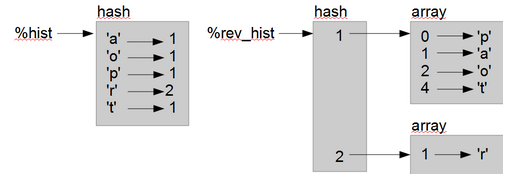
\includegraphics[scale=0.8]{figs/hash1.png}}
\caption{State diagram.}
\label{fig.hash1}
\end{figure}

Figure~\ref{fig.hash1} is a state diagram showing \verb'%hist'  and \verb'%rev-hist' .
A hash is represented as a box with the type {\tt hash} above it
and the key-value pairs inside.
\index{state diagram}
\index{diagram!state}

Arrays can be values in a hash, as this example shows, but they
cannot be keys.  If you try, you're likely to end up with a 
key that contains only one item of the array, but most likely 
not what you intended:

\begin{verbatim}
my @a = 'a' .. 'c';
my %h;
%h{@a} = 5;
say %h;  # -> a => 5, b => (Any), c => (Any)
\end{verbatim}

Here, Perl interpreted the \verb'%h{@a} = 5;' assignment 
as a a slice assignment, i.e., assumed that we were 
trying to populate three items in one go, one for each 
element of the array.

\index{hash!function}
\index{hashable}
As mentioned earlier, a hash is implemented using
a hashing function and that means that the keys have to 
be \emph{hashable} \footnote{This is not entirely true. The 
keys of a ``normal'' hash must be hashable and therefore 
immutable. There is another type of hash, object hashes, 
for which the need to have immutable keys does not apply.}. 
A {\bf hashing} is a function that takes 
a value (of any kind) and returns an integer.  Hashes use 
these integers, called hash values, to store and look up 
key-value pairs.
\index{immutability}

This system works fine if the keys are immutable.  But if the
keys are mutable, like with arrays, bad things would happen. For example,
when you create a key-value pair, Perl would hash the key and 
store it in the corresponding location.  If you modify the
key and then hash it again, it would go to a different location.
In that case, you might have two entries for the same key,
or you might not be able to find a key.  Either way, the
hash wouldn't work correctly.

That's why keys have to be hashable, and why mutable types like
arrays aren't. So Perl will do something else that can be 
useful (such as creating three distinct hash items in the 
example above), but will not hash the array itself.

Since hashes are mutable, they can't be used as keys,
but they {\em can} be used as values, so that you can 
have nested hashes.

\section{Memos}
\label{memoize}
\index{memoize}
\index{cache}
\index{memo}
\index{Fibonacci}

If you played with the {\tt fibonacci} subroutine from
Section~\ref{one.more.example}, you might have noticed that 
the bigger the argument you provide, the longer the 
subroutine takes to run. Furthermore, the run time 
increases extremely quickly.
\index{Fibonacci!function}
\index{function!Fibonacci}

To understand why, consider Figure~\ref{fig.fibonacci}, which shows
the {\bf call graph} for {\tt fibonacci} with {\tt n=4}.

\begin{figure}
\centerline
{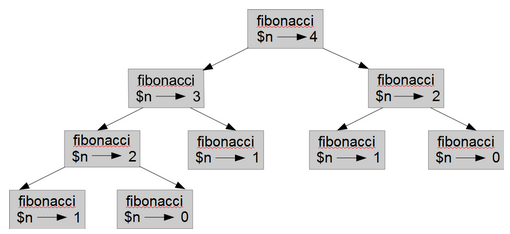
\includegraphics[scale=0.7]{figs/fibonacci.png}}
\caption{Call graph.}
\label{fig.fibonacci}
\end{figure}

A call graph shows a set of subroutine frames, with lines 
connecting each frame to the frames of the functions it 
calls.  At the top of the graph, {\tt fibonacci} with 
\verb'$n=4' calls {\tt fibonacci} with \verb'$n=3' and 
\verb'$n=2'.  In turn, {\tt fibonacci} with \verb'$n=3' calls
{\tt fibonacci} with \verb'$n=2' and \verb'$n=1'.  And so on.
\index{function frame}
\index{frame}
\index{call graph}

Count how many times {\tt fibonacci(0)} and {\tt fibonacci(1)} 
are called.  This is an inefficient solution to the problem, 
and it gets much worse as the argument gets bigger.
\index{memo}

One solution is to keep track of values that have already been
computed by storing them in a hash.  A previously computed value
that is stored for later use is called a {\bf memo}.  Here is a
``memoized'' version of {\tt fibonacci}:

\begin{verbatim}
my %known = 0 => 1, 1 => 1;
say fibonacci(10);
sub fibonacci ($n) {
    return %known{$n} if %known{$n}:exists;
    %known{$n} = fibonacci($n-1) + fibonacci($n-2);
    return %known{$n};
}
\end{verbatim}
%

\verb'%known' is a hash that keeps track of the Fibonacci
numbers we already know.  It starts with
two items: 0 and 1, which both map to 1.

Whenever {\tt fibonacci} is called, it checks \verb'%known'.
If the result is already there, it can return
immediately.  Otherwise, it has to 
compute the new value, add it to the hash, and return it.

If you run this version of {\tt fibonacci} and compare it with
the original, you will find that it is much faster, especially 
for a large argument (say more than 30).

\index{cache}
\index{memoize}
Memoizing is a form of \emph{caching}, i.e., storing in memory 
the result of a (presumably costly) computing operation in 
order to avoid computing it again. This process is 
sometimes called ``trading memory against CPU cycles.''  In 
some cases, such as our Fibonacci recursive example here, the gain 
can be absolutely huge: calculating the 100th Fibonacci 
number would take billions of years with the original recursive 
subroutine and it takes only a split second with the memoized 
version.

Please note that in the specific case of the Fibonacci function, 
we are storing values for each successive integer; we could 
have memoized the Fibonacci numbers in an array rather than 
in a hash (and it might even be slightly more efficient), but 
using a hash for such purpose is a more general solution, 
working even when the memo keys are not consecutive integers.

As an exercise, try to rewrite the {\tt fibonacci} subroutine 
using an array instead of a hash to memoize the calculated 
Fibonacci numbers.


\section{Hashes as Dispatch Tables}
\label{dispatch}

You may 
need a procedure to launch some action depending on the 
value of a parameter received by the program. To do that, 
you could use a series of 
\verb'if {...} elsif {...} else {...}' 
statements like this:

\begin{verbatim}
sub run-stop  { ... };
sub run-start { ... };
my $param = get-param;
if $param eq "stop" {
    run_stop;
} elsif $param eq "start" {
    run-start;
} elsif $param = "h" {
    say $help;
} elsif $param = "help" {
    say $help;
} elsif $param = "v" {
    $verbose = True;
} else {
    die "Unknown option $param";
}
\end{verbatim}

This approach is boring and error-prone. Using a dispatch table 
is often a simpler solution.

A dispatch table is a data structure mapping identifiers to 
code references or subroutine objects. Applied to the 
above scenario, it could look like this:

\begin{verbatim}
sub run-stop  { ... };
sub run-start { ... };
my %dispatch = (
    stop  => &run-stop,
    start => &run-start,
    h     => { say $help; },
    help  => { say $help; },
    v     => { $verbose = True;},
);
my $param = get-param();
die "Unknown option $param" unless %dispatch{$param}:exists;
%dispatch{$param}(); # execute the action specified in %dispatch
\end{verbatim}

The \verb'%dispatch' hash defines the action depending on 
the parameter used as a key. The \verb'%dispatch{$param}()' 
statement calls the required action.

This approach is a bit more concise and slightly cleaner, but there 
are some other advantages. It is more maintainable: if you need 
to add one option, you just need to add one entry to the hash 
and don't have to add code in the middle of a complicated 
chain of nested \verb'if {...} elsif {...} else {...}' 
statements at the risk of breaking up something. 

Another upside is that the dispatch table can be dynamically 
modified at run time, for example depending on certain 
external circumstances (for example the day in the month when 
the program is running) or in accordance with a configuration 
file. This means that it is possible to dynamically modify 
the behavior of a program after compile time, while it is 
already running. This paves the way to some very interesting 
advanced programming techniques that are beyond the scope 
of this book.

Note that we have been using hashes for our dispatch tables, 
and this is the most common way to implement them. If it 
makes sense to have small integers as keys, you could also 
implement a dispatch table as an array. This is the case, 
for example, with numbered menu items where the user is 
prompted to type a number to indicate which menu option 
to activate.


\section{Global Variables}
\index{global variable}
\index{variable!global}
\index{lexical variable}
\index{variable!lexical}

In the previous example, \verb'%known' is created outside the subroutine,
so it belongs to the whole main package.
Such variables are sometimes called {\bf global} 
because they can be accessed from any function.  Unlike ``local'' 
lexical variables, which usually disappear when their scope 
ends, global variables persist from one subroutine call to 
the next.
\index{flag}

It is common to use global variables for {\bf flags}; that is, 
boolean variables that indicate (``flag'') whether a condition
is true.  For example, some programs use a flag named 
\verb'$verbose' to control the level of detail in the
output:

\begin{verbatim}
my $verbose = True;
sub example1 {
    say 'Running example1' if $verbose;
    # ...
}
\end{verbatim}
%

Global variables are also sometimes used for environment 
variables and parameters passed to the program, as well
as for storing a large 
data structure that is the centerpiece of a program, in order 
to avoid copying it when passing it around as an argument to 
subroutines.

But, asides from those specific cases, it is usually 
considered poor practice to use a global variable, because 
it creates dependencies and unexpected ``action-at-a-distance'' 
behaviors between various parts of a program and may lead to 
difficult-to-track bugs.


\section{Debugging}
\index{debugging}

As you work with bigger datasets it can become unwieldy to
debug by printing and checking the output by hand.  Here are some
suggestions for debugging large data sets:

\begin{description}

\item[Scale down the input] If possible, reduce the size of the
dataset.  For example if the program reads a text file, start with
just the first 10 lines, or with the smallest example you can find.
You can either edit the files themselves, or (better) modify the
program so it reads only the first {\tt n} lines.

If there is an error, you can reduce {\tt n} to the smallest
value that manifests the error, and then increase it gradually
as you find and correct errors.

\item[Check summaries and types] Instead of printing and checking the
entire dataset, consider printing summaries of the data: for example,
the number of items in a hash or the total of a list of numbers.

A common cause of runtime errors is a value that is not the right
type.  For debugging this kind of error, it is often enough to print
the type of a value (think about the {\tt .WHAT} method).
\index{WHAT}

It is often useful to add typing to your variables. Where you 
expect a string, make sure you type the variable or subroutine 
parameter with {\tt Str}. If you expect an integer, type it with 
{\tt Int}. If you expect an {\tt Int} of a certain range, create 
a subset for it as in Section~\ref{guardian} (p.~\pageref{guardian}) 
and type the variable with that.
\index{subset!type}
\index{type subset}

\item[Write self-checks:]  Sometimes you can write code to check
for errors automatically.  For example, if you are computing the
average of a list of numbers, you could check that the result is
not greater than the largest element in the list or less than
the smallest.  This is called a ``sanity check'' because it detects
results that are ``insane.''
\index{sanity check}
\index{consistency check}

Another kind of check compares the results of two different
computations to see if they are consistent.  This is called a
``consistency check.''

\item[Format the output] Formatting debugging output
can make it easier to spot an error.  We saw an example in
Section~\ref{factdebug}.  The {\tt dd} function displays 
helpful details on a composite or complex data structure.

\index{dd function}
\index{function!dd}

\end{description}

Again, time you spend building scaffolding can reduce
the time you spend debugging.
\index{scaffolding}


\section{Glossary}

\begin{description}

\item[Mapping] A relationship in which each element of one set
corresponds to an element of another set.
\index{mapping}

\item[Hash] A mapping from keys to their
corresponding values.
\index{hash}

\item[key-value pair:] The representation of the mapping from
a single key to its value.
\index{key-value pair}

\item[Item] In a hash, another name for a key-value
  pair.
\index{item!hash}

\item[Key] An object that appears in a hash as the
first part of a key-value pair.
\index{key}

\item[Value] An object that appears in a hash as the
second part of a key-value pair.  This is more specific than
our previous use of the word ``value.''
\index{value}

\item[Implementation] A way of performing a computation.
\index{implementation}

\item[Hash table] The algorithm used to implement hashes.
\index{hashtable}

\item[Hash function] A function used by a hash table to 
compute the location of a key.
\index{hash!function}

\item[Hashable] A type that has a hash function.  Immutable
types like numbers and strings are hashable; mutable types 
like arrays and hashes are not.
\index{hashable}

\item[Lookup] A hash operation that takes a key and finds
the corresponding value.
\index{lookup}

\item[Reverse lookup] A hash operation that takes a value and finds
one or more keys that map to it.
\index{reverse lookup}

\item[Call graph] A diagram that shows every frame created during
the execution of a program, with an arrow from each caller to
each callee. 
\index{call graph}
\index{diagram!call graph}

\item[Memo] A computed value stored to avoid unnecessary future 
computation.
\index{memo}

\item[Global variable]  A variable defined outside any 
subroutine or other block.  Global variables can be 
accessed from any subroutine.
\index{global variable}

\item[Flag] A Boolean variable used to indicate whether a condition
is true.
\index{flag}

\end{description}


\section{Exercises}

\begin{exercise}
\label{wordlist2}
\index{set!membership}
\index{membership!set}

Write a subroutine that reads the words in \emph{words.txt} and
stores them as keys in a hash.  (It doesn't matter what the
values are.)  Then you can use the {\tt exists} adverb
as a fast way to check whether a string is in
the hash.

If you did Exercise~\ref{bisection}, you can compare the speed
of this implementation with a hash and the bisection search.

Solution: \ref{sol_wordlist2}

\end{exercise}


\begin{exercise}
\label{mem_ackerman}
Memoize the Ackermann function from Exercise~\ref{ackermann} 
and see if memoization makes it possible to evaluate the 
subroutine with bigger arguments.  Hint: no.
Solution: \ref{sol_mem_ackerman}.
\index{Ackermann function}
\index{function!ack}

\end{exercise}



\begin{exercise}
\index{duplicate}
\label{has_duplicates_hash}

If you did Exercise~\ref{has_duplicates}, you already have
a function named \verb"has-duplicates" that takes a list
as a parameter and returns {\tt True} if any object
appears more than once in the list.

Use a hash to write a faster, simpler version of
\verb"has-duplicates". 
Solution: \ref{sol_has_duplicates_hash}.

\end{exercise}


\begin{exercise}
\label{exrotatepairs}
\index{letter rotation}
\index{rotation, letters}

Two words are ``rotate pairs'' if you can rotate one of them
and get the other (see \verb"rotate_word" in 
Exercise~\ref{rotate}) using the Caesar cipher.
\index{Caesar cipher}

Write a program that reads a wordlist (e.g. {\tt words.txt} 
and finds all the rotate pairs.  
Solution: \ref{sol_exrotatepairs}.

\end{exercise}


\begin{exercise}
\label{homophones}
\index{Car Talk}
\index{Puzzler}

Here's another Puzzler from {\em Car Talk} 
(\url{http://www.cartalk.com/content/puzzlers}):

\begin{quote}
This was sent in by a fellow named Dan O'Leary. He came upon a common
one-syllable, five-letter word recently that has the following unique
property. When you remove the first letter, the remaining letters form
a homophone of the original word, that is a word that sounds exactly
the same. Replace the first letter, that is, put it back and remove
the second letter and the result is yet another homophone of the
original word. And the question is, what's the word?

Now I'm going to give you an example that doesn't work. Let's look at
the five-letter word, `wrack.' W-R-A-C-K, you know like to `wrack with
pain.' If I remove the first letter, I am left with a four-letter
word, 'R-A-C-K.' As in, `Holy cow, did you see the rack on that buck!
It must have been a nine-pointer!' It's a perfect homophone. If you
put the `w' back, and remove the `r,' instead, you're left with the
word, `wack,' which is a real word, it's just not a homophone of the
other two words.

But there is, however, at least one word that Dan and we know of,
which will yield two homophones if you remove either of the first two
letters to make two, new four-letter words. The question is, what's
the word?
\end{quote}
\index{homophone}
\index{reducible word}
\index{word, reducible}

You can use the hash from Exercise~\ref{wordlist2} above to check
whether a string is in {\tt words.txt}.

To check whether two words are homophones, you can use the CMU
Pronouncing Dictionary.  You can download it from
\url{http://www.speech.cs.cmu.edu/cgi-bin/cmudict}.
\index{CMU Pronouncing Dictionary}

Write a program that lists all the words in {\tt words.txt} 
(or in the CMU dictionary) that solve the Puzzler.
Solution: \ref{sol_homophones}.

\end{exercise}





\chapter{Case Study: Data Structure Selection}
\label{data_struct_sel}

At this point you have learned about Raku's core data structures,
and you have seen some of the algorithms that use them.

This chapter presents a case study with exercises that let
you think about choosing data structures and practice using them.

But first, I would like to briefly introduce two conditional 
structures that have been left aside so far and provide 
a couple of new possibilities about subroutine signatures. 
\index{signature}

\section{The Ternary Conditional Operator}
\label{ternary operator}
\index{ternary conditional operator}

Consider the following code that tests the value of a positive 
integer:

\begin{verbatim}
my $result;
if $num < 10 {
    $result = "One digit";
} else {
    $result = "More than one digit";
}
say $result;
\end{verbatim}

This is quite simple, but a bit long. This can be rewritten 
in just one line of code:

\begin{verbatim}
say $num < 10 ?? "One digit" !! "More than one digit";
\end{verbatim}

The operator is in two parts: the {\tt ??} and the {\tt !!}, which 
separate three expressions (hence the name ``ternary operator''): 
\index{ternary operator}
\index{operator!ternary}
\begin{itemize}
\item The condition to be evaluated (is \verb'$num' less than 10?);
\item The expression defining the value if the condition is true;
\item The expression defining the value if the condition is false.
\end{itemize}

This statement checks if \verb'$num' is less than 10 and, if 
true, prints ``"One digit;'' if the 
condition is false, it prints ``More than one digit.''

This operator does not provide any new functionality; it just 
offers a more concise syntax.

It is possible to nest several ternary operators to examine 
successively multiple choices:
\index{ternary conditional operator, nesting}

\begin{verbatim}
say $value < 10    ?? "One digit"     !! 
    $value < 100   ?? "Two digits"    !!
    $value < 1000  ?? "Three digits"  !!
                      "More than three digits";
\end{verbatim}

This construct is a form of what is sometimes called a 
\emph{switch statement}, because the C language and 
many languages derived from it use the {\tt switch} keyword 
to describe such a multiple choice conditional.
\index{switch statement}

This is much more concise and often more convenient than nested 
{\tt if ... then ... else} conditionals, but the next section 
provides a more powerful {\tt switch} type of statement.

\section{The {\tt given ... when} ``Switch'' Statement}
\label{given_when}
\index{given statement}
\index{when statement}
\index{switch statement}

Raku has a ``switch'' statement, written with the 
{\tt given} and {\tt when} keywords. The 
{\tt given} keyword introduces the variable or expression 
that will be tested, and each of the {\tt when} 
statements specify a condition followed by a block that 
will execute if the condition is true. By default, the 
process stops at the first condition that is satisfied.

The example just above can be rewritten as follows:

\begin{verbatim}
given $value {
    when 0..9      { say "One digit" }
    when $_ < 99   { say "Two digits" }
    when /^\d**3$/ { say "Three digits" }
    default        { say "More than three digits" }
}
\end{verbatim}

The \verb'given $value' statement ``topicalizes'' the argument, 
i.e., assigns the content of  \verb'$value' to the \verb'$_' 
topical variable (or, more precisely, aliases it to \verb'$_'). 
The argument to {\tt given} is a simple variable in the 
example above, but it can be a complex expression whose 
evaluation is stored (and cached) into \verb'$_'. 
Each of the {\tt when} conditions is checked against \verb'$_'. 
I have written these conditions in three different syntactical 
forms to illustrate some of the various possibilities:
\index{topical variable}
\index{alias}
\begin{itemize}
\item The first one checks \verb'$_' (implicitly) against 
the \verb'0..9' range.
\index{range operator}
\item The second one compares explicitly \verb'$_' to 99.
\item The third one uses a regex to check whether \verb'$_' has 
three digits.
\index{regex}
\item The \verb'default' statement runs only if the other 
conditions have failed.
\index{default statement}
\end{itemize}

Only one message will be printed, because the 
matching process stops as soon as one condition has been 
satisfied, and the \verb'default' clause will run if 
no other condition has been met.

If there is no specific operator in the {\tt when} clause, 
then it will smart match the expression in the {\tt when} 
clause against \verb'$_':
\index{smart match}

\begin{verbatim}
when $foo { ... }
# equivalent to: when $foo ~~ $_ { ... }
\end{verbatim}

Note that the {\tt given} keyword is not doing much more than 
topicalizing its argument for the rest of the block. 
The {\tt when} clauses are doing the bulk of the real work. In fact, 
you could even use the {\tt when} clauses without a {\tt given}, 
provided you assign the right value to \verb'$_', which, as you 
hopefully remember, can be done with a {\tt for} block:
\index{for block}

\begin{verbatim}
my $val = 7;
for $val { 
    when 0..6 { say "less than"}
    when 7 {say "Exact";} 
    when 8..* {say "greater than";}
}
\end{verbatim}

\index{proceed clause}
It is possible to add a {\tt proceed} clause at the end of 
any of the conditional code blocks to prevent the process 
from stopping after that code block has succeeded. For example, 
you might write this:

\begin{verbatim}
given $value {
    when 0..9      { say "One digit"}
    when 10..99    { say "Two digits"; proceed}
    when 42        { say "The response to the ultimate question"}
    when /^\d**3$/ { say "Three digits" }
    default        { say "More than three digits" }
}
\end{verbatim}

Here, if \verb'$value' is 42, two messages will be displayed,  
``Two digits'' and ``The response to the ultimate question,'' 
because the {\tt proceed} clause in the second code block 
prevents the process from stopping on the first successful match.

Good, it seems, but there is a problem. The {\tt proceed} clause 
should be used with some care, as it can easily lead 
to unexpected results. In fact, \emph{the code above 
is actually wrong}: if \verb'$value' has two digits but is 
not 42 (if it is, say, 43), the default block will also run, 
because the only other successful match had this {\tt proceed} 
clause, and will say that there are ``More than three digits'' 
although this is obviously false. 

\label{proceed_ex}
As an exercise, test the above code with various values and 
try to find a way to fix the bug with the {\tt proceed} 
clause.

Solution: \ref{sol_proceed_ex}

\section{Multiple Conditionals with Junctions}
\label{junction}
\index{junction}

Sometimes, you need to test several possible conditions 
and would write something like this:

\begin{verbatim}
if $value == 3 or $value == 5 or $value == 7 { #...
\end{verbatim}

This is quite verbose, and I don't like to have to 
repeat the \verb'$value ==' part several times. I 
would prefer to be able to write something like: 
``If value is 3 or 5 or 7.'' That syntax doesn't work, 
but junctions enable you to do almost that:

\begin{verbatim}
if $value == 3|5|7 {
	say "$value is either 3, or 5, or 7"
}
\end{verbatim}

The \verb'3|5|7' part is a junction.

Junctions are superpositions of unordered values. 
Operations on junctions are executed for each item 
of the junction separately (and maybe even in parallel), 
and the results are assembled in a junction of the same 
type.

The junction types differ when evaluated in boolean context. 
The types and associated junction constructors are 
\verb'any', \verb'all', \verb'one' and \verb'none'.
\index{any junction}
\index{all junction}
\index{none junction}
\index{one junction}

\begin{table}[htb]%
\centering%
\begin{tabular}{llcl}
\toprule%
\textbf{Type} & \textbf{Constructor} & \textbf{Infix Operator}  & \textbf{True if...}                               \\\midrule
any           & any                  & \verb'|'                  & at least one value evaluates to \verb|True|      \\
all           & all                  & \verb'&'                  & no value evaluates to False \verb|False|         \\
one           & one                  & \verb'^'                  & exactly one value evaluates to True \verb|True|  \\
none          & none                 &                           & no value evaluates to \verb|True|                \\\bottomrule
\end{tabular}
\end{table}

\index{junction types}

For example, \verb'3|5|7' is the same as \verb'any(3, 5, 7)'.

This is another example of an \verb'any' junction:

\begin{verbatim}
my Junction $weekday = any <Monday Tuesday Wednesday 
                            Thursday Friday>
if $day eq $weekday {
    say "This is a weekday";
}
\end{verbatim}

In this example the \verb'eq' operator is called with each 
pair \verb'$day', 'Monday', \verb'$day', 'Tuesday', etc. 
and the result is put into an any-junction again. As 
soon as the result is determined (in this case, as soon 
as one comparison returns True), it can abort the 
execution of the other comparisons.

This works not only for operators, but also for routines:

\begin{verbatim}
if 2 == sqrt(4 | 9 | 16) {
    say "YaY";
}
\end{verbatim}

Junctions can be very handy to perform fairly common tasks. 
Imagine you have an array of numbers, and you want to 
check that all of them are non-negative. In most 
programming languages, you would write a loop to 
iterate over the array and check each item in turn. 
In Raku, this is very simple:

\begin{verbatim}
my @values = get-values();
if all(@values) >= 0 { ... }
\end{verbatim}

Or, if you want to avoid a division by zero exception:

\begin{verbatim}
my @values = get-values();
perform-division(@values) if none(@values) == 0;
\end{verbatim}
\index{junction}

\section{Subroutine Named and Optional Parameters}

The subroutines that we have seen so far used \emph{positional} 
parameters, i.e., parameters whose binding with the subroutine 
call arguments rely on their order within the list of 
arguments and in the signature. This is usually fine when 
the number of arguments passed to the subroutine is small 
(say, three or less). 
\index{positional parameter}
\index{parameter!positional}
\index{signature}

When the subroutine signature becomes longer, using positional 
arguments might become cumbersome and error-prone. 

\subsection{Named Parameters}
\label{named_parameters}
\index{named parameter}
\index{parameter!named}

Named arguments may be supplied in any order: the name of 
the parameter is bound to the argument having the same 
name. For example:

\begin{verbatim}
sub divide (:$dividend, :$divisor where $divisor != 0) {
     return $dividend/$divisor;
}
say divide(dividend => 2048, divisor => 128);      # -> 16
# or:
say divide(divisor => 128, dividend => 2048);      # -> 16
\end{verbatim}

The arguments are supplied at the subroutine call as a list of 
pairs using the pair-constructor syntax. In the signature, 
the parameters are retrieved with the 
so-called colon-pair syntax: the \verb'$dividend' parameter is 
bound to the value of the pair whose key is ``dividend'' (2048), 
and \verb'$divisor' is similarly bound to 128, irrespective of 
the order of the arguments in the subroutine call.
\index{colon-pair syntax}
\index{pair constructor}

These named parameters are especially useful when the number of 
arguments is large. For example, we haven't covered 
object-oriented programming yet (see Chapter~\ref{objects}), 
but this is how we could create an object of the 
(user-defined) Rectangle class:

\begin{verbatim}
my $rect = Rectangle.new( 
    origin_x  => 100, 
    origin_y  => 200, 
    width     => 23,
    length    => 42,
    color     => 'black'
);
\end{verbatim}

Clearly, using five positional parameters would be unpractical. 

\subsection{Optional Parameters}
\index{optional parameter}
\index{parameter!optional}
\index{variadic subroutine}
\index{signature}

Sometimes, the actual number of arguments is not known 
in advance: for example, a subroutine may be called with 
a variable number of arguments. Such a subroutine is said 
to be \emph{variadic}. You can define a parameter to be 
optional by postfixing it with a question mark in the 
subroutine signature:

\begin{verbatim}
sub my-sub($x, $y?) {  # simple optional parameter
    if $y.defined {
        say "The second parameter has been supplied and defined";
    } else {
        say "The second parameter has not been supplied";
    }
    # ...
}
\end{verbatim}

\index{positional parameter}
\index{parameter!positional}
When using positional parameters, the optional parameters 
always have to be the last ones in the list (after the 
mandatory ones).

A parameter can also be made optional by supplying a 
{\bf default value}:
\index{default value}
\index{default parameter}
\index{parameter!default value}

\begin{verbatim}
sub my-log($number, $base = e) {    # e is a predefined constant
                                    # $base is an optional parameter
    return log($number) / log($base);
}
say my-log(4);       # Natural log (base e)    -> 1.38629436111989
say my-log(32, 2);   # Log base 2              -> 5
say my-log(100, 10); # Common log (base 10)    -> 2
\end{verbatim}

Here, if the second argument is not supplied, the default 
value (\emph{e}) is used instead. Conversely, if there 
is a second argument, it {\bf overrides} the default value.

\index{slurpy parameters}
\index{parameter!slurpy}
\label{slurpy_parameters}
Sometimes, having optional or default parameters is not good 
enough. For example, the subroutine may have to process a list 
containing any number of values. For situations like this, 
you can use a \emph{slurpy parameter}, i.e., a kind of array 
placed at the end of the parameter list that will slurp up 
all the remaining arguments. This kind of slurpy parameter 
uses the ``\verb"*@"'' twigil. In the following example, 
the subroutine takes one mandatory parameter (the first 
number of the list) and a list of additional arguments 
that will be stored in the \verb'@rest' array:
\index{twigil}

\begin{verbatim}
sub my-sum($first-num, *@rest) {
    say @rest;                      # -> [3 4 5 12 17]
    return $first-num + [+] @rest;
}
say my-sum 1, 3, 4, 5, 12, 17;      # -> 42 
\end{verbatim}

Some further examples of slurpy parameters have been 
provided in Section~\ref{sol_exercise_queue}.

\section{Word Frequency Analysis}
\label{analysis}

Now, let's get to the case study.

As usual, you should at least attempt the exercises
before you read the suggested solutions, which are 
provided in the following sections of this chapter.

\begin{exercise}

Write a program that reads a file, breaks each line into
words, strips whitespace and punctuation from the words, and
converts them to lowercase.

\end{exercise}


\begin{exercise}
\index{Project Gutenberg}

Go to Project Gutenberg (\url{http://gutenberg.org}) and download 
your favorite out-of-copyright book in plain text format.
\index{plain text}
\index{text!plain}

Modify your program from the previous exercise to read the book
you downloaded, skip over the header information at the beginning
of the file, and process the rest of the words as before.

Then modify the program to count the total number of words in
the book, and the number of times each word is used.
\index{word frequency}
\index{frequency!word}

Print the number of different words used in the book.  Compare
different books by different authors, written in different eras.
Which author uses the most extensive vocabulary?
\end{exercise}


\begin{exercise}

Modify the program from the previous exercise to print the
20 most frequently used words in a given book.

\end{exercise}


\begin{exercise}

Modify the previous program to read a word list (see
Section~\ref{wordlist}) and then print all the words in the book that
are not in the word list.  How many of them are typos?  How many of
them are common words that {\em should} be in the word list, and how
many of them are really obscure?

\end{exercise}


\section{Random Numbers}
\index{random number}
\index{number, random}
\index{deterministic}
\index{pseudorandom}

Given the same inputs, most computer programs generate the same
outputs every time, so they are said to be {\bf deterministic}.
Determinism is usually a good thing, since we expect the same
calculation to yield the same result.  For some applications, though,
we want the computer to be unpredictable.  Games are an obvious
example, but there are more.

Making a program truly nondeterministic turns out to be difficult,
but there are ways to make it at least seem nondeterministic.  One of
them is to use algorithms that generate {\bf pseudorandom} numbers.
Pseudorandom numbers are not truly random because they are generated
by a deterministic computation, but just by looking at the numbers it
is all but impossible to distinguish them from random.

Raku provides functions such as {\tt rand} that generate
pseudorandom numbers (which we will simply call ``random'' 
numbers from here on).
\index{rand function}
\index{function!rand}

The function {\tt rand} returns a random number (of {\tt Num} 
type) between 0.0 and 1.0 (including 0.0 but not 1.0).  Each time you
call {\tt rand}, you get the next number in a long series.  To see a
sample, run this loop in the REPL:

\begin{verbatim}
say rand for 1..5;
\end{verbatim}

Used as a method, {\tt rand} returns a random number between 
0.0 and the value of the invocant. For example, {\tt 10.rand} 
returns a random number between 0 and 10 (10 not included). You
might try it as a one-liner:
\index{one-liner mode}

\begin{verbatim}
$ raku -e 'say 10.rand for 1..5'
8.23987158729588
9.83276889381497
2.52313276833335
3.44713459548771
1.82329894347025
\end{verbatim}
 
You should hopefully get a different output than I did. If 
you want to run such a one-liner under Windows, remember 
that you'll need to replace single quotes with double quotes.

To obtain random integers between 1 and 10, you may use 
the {\tt Int} and {\tt rand} methods:
\index{Int function or method}

\begin{verbatim}
$ raku -e 'say 10.rand.Int + 1 for 1..5'
5
10
1
6
3
\end{verbatim}

The {\tt pick} function or method takes a number \verb'$count'  and a list as arguments and returns \verb'$count' items chosen at 
random and without repetition. For example:
\index{pick function or method}

\begin{verbatim}
> say <1 3 4 5 7 9 10 12 14 42>.pick(5);
(5 42 3 4 7)
> say pick 5, <1 3 4 5 7 9 10 12 14 42>;
(42 12 5 1 9)
\end{verbatim}

If \verb'$count' if greater than or equal to the number of 
items of the list, then all elements from the list are returned 
in a random sequence.

To obtain random unique integers in a range, you might use 
{\tt pick} on a range:

\begin{verbatim}
> say pick 5, 1..20;
(5 3 6 18 7)
> say (1..20).pick(5);
(20 4 18 2 7)
\end{verbatim}

If you don't specify the number of random numbers, you'll get one 
random pick:

\begin{verbatim}
> say (1..20).pick;
19
\end{verbatim}
%


\begin{exercise}
\index{histogram!random choice}

Write a function named \verb"choose_from_hist" that takes
a histogram as defined in Section~\ref{histogram} and returns a 
random value from the histogram, chosen with probability
in proportion to frequency.  For example, for the three 
items: \verb"('a', 'a', 'b')", your function should 
return \verb"'a'" with probability $2/3$ and \verb"'b'" 
with probability $1/3$.
\end{exercise}


\section{Word Histogram}

You should attempt the previous exercises before you go on.

For the purpose of presenting the solutions to the above 
exercises, I've used the plain text of {\em Emma} (1816), the 
novel by Jane Austen, downloaded from the Gutenberg project 
(\url{http://www.gutenberg.org/files/158/158-0.txt}) and 
saved in a file called \emph{emma.txt} \footnote{The Gutenberg 
project slightly modified the format of this file after this 
chapter was written. To avoid any problem associated with this 
change (and any other future changes), you can download the 
original file from my Github repository: 
\url{https://github.com/LaurentRosenfeld/think_raku/blob/master/Supplementary/emma.txt}.} Use the same 
text if you want to compare your solutions and results 
with mine.
\index{Austin, Jane}
\index{Emma}
\index{Project Gutenberg}

Here is a program that reads the \emph{emma.txt} file and 
builds a histogram of the words in the file:
\index{histogram!word frequencies}

\begin{verbatim}
my %histogram;
my $skip = True; # flag to skip the header

sub process-line(Str $line is copy) {
    if defined index $line, "*END*THE SMALL PRINT!" {
        $skip = False ;
        return;
    }
    return if $skip;
    $line ~~ s:g/<[-']>/ /; # Replacing dashes and apostrophes with spaces
    $line ~~ s:g/<[;:,!?.()"_`]>//; # removing punctuation symbols
    $line = $line.lc;               # setting string to lower case
    for $line.words -> $word {
        %histogram{$word}++;
    }
	$skip = True if $line ~~ /^finis$/;
}
process-line $_ for "emma.txt".IO.lines; 
\end{verbatim}
\index{case!lower}
%

The program reads each line of the \emph{emma.txt} file and, for 
each line, calls \verb"process-line". 

\index{accumulator!histogram}
The \verb"process-line" subroutine skips the header lines 
(i.e., all the lines until a line containing the string
``*END*THE SMALL PRINT!'' 
is met \footnote{This line is no longer present in the new version of 
the Emma file currently on the Gutenberg project site. So this will 
work only with my version of this file on my Github repository:  
\url{https://github.com/LaurentRosenfeld/think_raku/blob/master/Supplementary/emma.txt}.}). It replaces dashes and apostrophes with spaces, removes 
various punctuation characters, and sets the line to lower case. 
Finally, it splits the line into individual words that are 
stored and counted with an accumulator in the \verb'%histogram' 
hash.

To know whether the program is doing something like what 
it is supposed to do, we can display a few entries of the 
\verb'%histogram' hash:

\begin{verbatim}
# displaying 20 lines of the histogram
my $count;
for %histogram -> $pair {
    say sprintf "%-24s %d", $pair.key, $pair.value;
    $count++;
    last if $count > 20;
}
\end{verbatim}

This prints out the following output:

\begin{verbatim}
embarrassing             1
hows                     1
appealed                 2
bestow                   2
articulate               1
demands                  2
closely                  1
dull                     9
hearts                   1
column                   1
possesses                1
attributed               1
jumped                   2
forwards                 2
wittier                  2
expert                   2
attractive               2
asserted                 2
oftentimes               1
fancy                    38
finds                    1
\end{verbatim}


To count the total number of words in the file, we can add up
the values in the histogram:

\begin{verbatim}
my $word_count = [+] %histogram.values;
say "There are $word_count words in the book.";
\end{verbatim}
%
The number of different words is just the number of items in
the hash:

\begin{verbatim}
my $distinct-words = %histogram.elems;
say "There are $distinct-words distinct words in the book.";
\end{verbatim}
%
Note that you could reduce the above to one code line by 
interpolating a code block within the output string:
\index{interpolating a code block in a string}

\begin{verbatim}
say "There are {%histogram.elems} distinct words in the book."
\end{verbatim}
%
And the results:

\begin{verbatim}
There are 161991 words in the book.
There are 7110 distinct words in the book.
\end{verbatim}
%


\section{Most Common Words}
\label{most_common_words}

To find the most common words in \verb'emma.txt', we can 
sort the \verb'%histogram' hash according to the values 
(word frequencies) and retrieve the 10~most frequent words 
into an array.
\index{sort}

\begin{verbatim}
my @most_commons = (sort { %histogram{$^b} cmp %histogram{$^a} }, 
                    %histogram.keys)[0..9];
say $_ for map { "$_ \t%histogram{$_} "}, @most_commons;
\end{verbatim}

The {\tt sort} functions receives the keys of the histogram and 
its comparison function compares the values associated with 
those keys. Since we use the key \verb'$^b' before the key 
\verb'$^a', the sort will produce a reverse (descending) sort 
order. The whole {\tt sort} procedure is placed within parentheses, 
so that the subscript range {\tt [0..9]} acts as a slice on 
the list produced by {\tt sort} and retains only the first 10~most 
frequent words. The result is stored into the 
\verb'@most_commons' array. The next code line just reprocesses 
the array to display the words and their respective frequency.
\index{slice}

This displays the following output:

\begin{verbatim}
to      5241
the     5205
and     4897
of      4295
i       3192
a       3130
it      2529
her     2490
was     2400
she     2364
\end{verbatim}
%
If you want to see more interesting words, you might, as a
further exercise, filter the histogram and retain only 
words that have more than, say, four letters.

The \verb'@most_commons ' temporary array is not really needed. 
We could do the whole thing in a single statement:

\begin{verbatim}
say $_ for map { "$_ \t%histogram{$_} "},  
           (sort { %histogram{$^b} cmp %histogram{$^a} }, 
           %histogram.keys)[0..9];
\end{verbatim}

This is an example of data pipeline (or stream) programming. Such a statement 
needs to be read from bottom to top and from right to left. The 
first step is \verb'%histogram.keys', which produces a list 
of the histogram keys; this list is fed into the sort statement 
to produce a list of the keys sorted (in descending order) according 
to their values; once this whole part between parentheses is 
completed, the subscript range \verb'[0..9]' retains the 
10~most frequent words and feeds them into the map statement, 
which produces the list of words and frequencies for the final 
output.

Let me add one word of caution here: sorting the histogram by 
values and picking up the top 10 to get the most frequent 
words is probably the easiest way to solve the problem and the 
shortest code to do it. That's the reason I have used this 
solution here. But it is not the most efficient solution 
from the standpoint of the run time, because it involves the 
cost of sorting a relatively large data set, whereas we are 
using only a small part of the sorted data. There are some 
better algorithms to do that from the standpoint of runtime 
efficiency, but they are more complicated. So, there is a 
tradeoff here between coding efficiency and performance. 
Assuming this is code that we want to run only once, I have 
chosen to favor coding efficiency.

\index{data pipeline programming}


\section{Optional Parameters}
\index{optional parameter}
\index{parameter!optional}

We saw earlier in this chapter that subroutines can 
take optional parameters. We can use this functionality to 
write a subroutine that prints the most common words in the 
\verb'%histogram' hash extracted from \emph{emma.txt}.

\begin{verbatim}
display-most-common(%histogram, 5);

sub display-most-common (%hist, Int $num = 10) {
    say $_ for map { "$_ \t%hist{$_} "}, 
    (sort { %hist{$^b} cmp %hist{$^a} },
    %hist.keys)[0..$num - 1];
}
\end{verbatim}

This will display the five top words of the list above 
(Section~\ref{most_common_words}). If we call it without 
the second parameter:

\begin{verbatim}
display-most-common(%histogram);
\end{verbatim}

we will get the 10~most common words (same list as the one 
shown in Section~\ref{most_common_words} above), because 
the default value for the second parameter is 10.


\section{Hash Subtraction}
\label{hashsub}
\index{hash!subtraction}
\index{subtraction!hash}

Finding the words from \emph{emma.txt} that are not in the word list
{\tt words.txt} is a problem you might recognize as set
subtraction; that is, we want to find all the words from one
set (the words in \emph{emma.txt}) that are not in the other (the
words in \emph{words.txt}).

{\tt subtract} takes hashes \verb'%main' and \verb'%dict' and 
returns a new hash that contains all the keys from \verb'%main' 
that are not in \verb'%dict'.  Since we don't really care about 
the values, we set them all to 1:

\begin{verbatim}
sub subtract (%main, %dict) {
	my %difference;
	for %main.keys -> $word {
		%difference{$word} = 1 unless %dict{$word}:exists;
	}
	return %difference;
}
\end{verbatim}
%
To find the words in \emph{emma.txt} that are not in  \emph{words.txt},
we need to load the word list into a hash and to call 
{\tt subtract}, passing the two hashes as arguments. We also 
add some code to print the first 20~words not found in the 
word list:

\begin{verbatim}
my %word-list = map { $_ => 1 }, "words.txt".IO.lines;
my %unknown-words = subtract(%histogram, %word-list);
say %unknown-words.keys.head(20);
\end{verbatim}
%
\index{head}
Notice that rather than using a subscript slice, I have used 
here the {\tt head} method to print out the first 20~words of 
the list. This is just another way to get the first ``n'' items 
of a list or array. There is also a {\tt tail} method to 
retrieve the last ``n'' items of a list or an array.
\index{head method}
\index{tail method}

Here are some of the results from {\em Emma}:

\begin{verbatim}
(penetrated unsullied bateses outstepped particularity experienced 
italian sunday solicitously blockhead unbleached ult 26th 
christian 7th untouched iii greensward houseroom tete)
\end{verbatim}
%
Some of these words are names and ordinal numbers.  Others 
are rare or no longer in common use.  But a few are common
words that should really be in the list!

Note that I have used a hash (\verb'%unknown-words') here to 
store the words of \emph{emma.txt} not found in the word list. 
Since we are using the data only to print a sample of 20 words, 
we could have used an array as well.

\section{Constructing New Operators}

\label{operator_construction}
\index{hash!subtraction}
\index{creating new operators}
\index{new operators!creating}
\index{overload operators}
\index{operator!overloading}
\index{operator construction}

Learning about hash subtraction is an excellent 
opportunity to introduce a very interesting functionality of 
Raku: the capacity to construct new operators or to 
redefine existing ones.

Since we are subtracting two lists of words, it is tempting to 
use the minus sign to denote this subtraction operation. It  
is very easy to create such an operator in Raku:

\begin{verbatim}
multi sub infix:<-> (%main, %dict) {
	my %difference;
	for %main.keys -> $word {
		%difference{$word} = 1 unless %dict{$word}:exists;
	}
	return %difference;
}
\end{verbatim}

\index{infix}
\index{subroutine signature}
\index{signature}
\index{multi!subroutine}

Compared to the definition of the {\tt subtract} subroutine, the 
only differences are in the header line. We will cover the 
details in a later chapter, but let us briefly explain here.
Most Raku operators are defined as ``multi'' subroutines, 
i.e., subroutines that can be defined several times with 
different signatures and bodies; Raku will know which one to use depending 
on the signature. Here we define the minus operator as a 
multi subroutine whose parameters are two hashes; this will be 
enough for the Raku compiler to know that we don't want 
the regular subtraction between numerical values, but something 
else that applies to two hashes. The minus operator is defined as 
``infix,'' which means that the operator will be placed 
between its two operands.

Calling this new operator is now just as easy as calling 
the regular subtraction operator between numbers; we just need 
to use two hashes as operands:

\begin{verbatim}
my %unknown-words = %histogram - %word-list;
\end{verbatim}

The rest of the program works just as before.

\index{extending the language}
This ease or creating new operators is one of the facilities 
offered by Raku to \emph{extend the language} from within itself. 
We'll come back to that and other ways to extend the language 
in later chapters.

\label{fact_operator}
\index{factorial}
\index{factorial!operator}
As an exercise, write a multi subroutine that creates the new 
postfix ``!'' operator for computing the factorial of an integer:
\index{factorial}

\begin{verbatim}
say 5!;     # -> 120
\end{verbatim}
%
Also try to think about how you would test this new ``!'' operator 
against various input values.
Solution: \ref{sol_fact_operator}


\section{Sets, Bags and Mixes}
\label{sets_and_bags}

\index{set}
\index{type!set}
\index{bag}
\index{type!bag}
\index{mix}
\index{type!mix}
\index{sethash}
\index{type!sethash}
\index{baghash}
\index{type!baghash}
\index{mixhash}
\index{type!mixhash}

Raku has a variety of data structure types called {\tt Set}, 
{\tt Bag} and {\tt Mix} that provide many common set 
operations. They are unordered collections of unique and 
weighed items. They are immutable (but there also exist mutable 
versions of these data structures, {\tt SetHash}, {\tt BagHash} 
and {\tt MixHash}).

You may create and use a set as follows:

\begin{verbatim}
> my $s = set <banana apple orange orange banana pear apple>;
set(banana, orange, apple, pear)
> say $s.perl
set("banana","orange","apple","pear")
> say $s.elems;
4
> say $s{'apple'}
True
> say $s{'strawberry'}
False
\end{verbatim}
%
As you can see, duplicates have been removed. Sets only tell us 
whether or not at least one item of a given name has been seen.

A bag, by contrast, also keeps track of how many of each items 
have been seen:

\begin{verbatim}
> my $b = bag <banana apple orange orange banana pear apple orange>;
bag(banana(2), orange(3), pear, apple(2))
> say $b{'banana'}
2
\end{verbatim} 

Mixes are similar to bags, except that the elements' weights don't 
have to be integers.

The interesting thing about these collections is that they can use 
many set operators commonly used in mathematics, such as the 
\verb'∈' set membership operator (or use \verb'(elem)' instead 
if you don't know how to type \verb'∈' in your 
editor~\footnote{I can't teach you here how to type these characters, 
because each editor will require a different method.}), the \verb'∩' or 
\verb'(&)' set intersection operator, or the \verb'⊂' or 
\verb'(<)' subset operator:

\begin{verbatim}
> say "Found it!" if 'apple' ∈ $s;
Found it!
> say "Is subset!" if <orange banana> ⊂ $s;
Is subset!
> say <orange banana pineapple> ∩ $s;
set(banana, orange)
\end{verbatim}

Notice that we haven't used the {\tt set} keyword to define the 
\verb'<orange banana>' list in the second example above. This list 
has been coerced to a {\tt Set} to check whether it was a subset 
of the \verb'$s' set. This is one of the great things about these 
collections: most of these set operators can be used with lists, 
arrays, and hashes.
\index{coercion}

\index{set!membership operator}
\index{operator!set membership}
We can rewrite the hash subtraction program using a set for 
the word list and the  \verb'∈' (or \verb'(elem)') 
set membership operator:

\begin{verbatim}
my %histogram;
my $skip = True; # flag to skip the header
sub process-line(Str $line is copy) {
    # (same as above)
}

process-line $_ for "emma.txt".IO.lines; 
my $word-list = set "words.txt".IO.lines;
my %unknown-words = subtract(%histogram, $word-list);
say %unknown-words.keys.head(20);

sub subtract (%main, $dict) {
	my %difference;
	for %main.keys -> $word {
		%difference{$word} = 1 unless $word ∈ $dict;
	}
	return %difference;
}
\end{verbatim}

The code line in the {\tt for} loop could also be written as follows:

\index{set!contain operator}
\index{operator!set contain}
\begin{verbatim}
        %difference{$word} = 1 unless $word (elem) $dict;
#or:    %difference{$word} = 1 if $word ∉ $dict;
#or:    %difference{$word} = 1 if $word !(elem) $dict;
#or even with the (cont) or ∋ contain operator:
        %difference{$word} = 1 unless $dict (cont) $word;
#or:    %difference{$word} = 1 unless $dict ∋ $word;
#or:    %difference{$word} = 1 if $dict ∌ $word;
# etc.
\end{verbatim}

\index{set!difference operator}
\index{operator!set difference}
The \verb'∖' \footnote{~Note that this is unicode character {\tt 2216}, 
not the same as the $\backslash$ backslash} and \verb'(-)' built-in operators 
provide a set difference, so that we needed neither to write a 
{\tt subtract} subroutine nor to construct our own minus operator:

\begin{verbatim}
process-line $_ for "emma.txt".IO.lines; 
my $word-list = set "words.txt".IO.lines;
my $unknown-words = %histogram.keys (-) $word-list;
say $unknown-words.keys.head(20);
\end{verbatim}

There are more than 30~set operators available, covering most of 
the set operators used in mathematics. I've only shown 
some that are the most likely to be useful. Check into the 
official documentation (\url{https://doc.raku.org/language/setbagmix}) 
if you need some others.

\label{diff_with_set}
As an exercise, you may rewrite the {\tt process-line} 
subroutine or replace it to use a set or a bag instead of a hash 
to store the words of \emph{emma.txt} (and possibly adapt the rest of 
the program where needed), in order to find the words of the \emph{emma.txt} 
that are not in the \emph{words.txt}.
Solution: \ref{sol_diff_with_set}


\section{Random Words}
\label{randomwords}
\index{histogram!random choice}

To choose random words from the histogram, the simplest algorithm
is to build a list with multiple copies of each word, according
to the observed frequency, and then choose from the list with the 
\verb'pick' function:
\index{pick function or method}

\begin{verbatim}
my @array = map {| (.key xx .value)}, %histogram;
say pick 30, @array;
\end{verbatim}
%
The expression \verb'map {| (.key xx .value)}' reads each 
pair of the histogram and creates a list with {\tt .value} 
copies of the string in {\tt key}.  The {\tt pick} function 
selects 30 random words from the array.

This algorithm works, but it is not very efficient; each time you
choose one or some random words, it rebuilds the list, which is 
as big as the original book.  An obvious improvement is to build 
the list once and then make multiple selections, but the list 
is still big.

An alternative is:

\begin{enumerate}

\item Use {\tt keys} to get a list of the words in \emph{emma.txt}.
\index{keys function}

\item Build a list that contains the cumulative sum of the word
  frequencies (see Exercise~\ref{cumulative}).  The last item
  in this list is the total number of words in the book, $n$.
  
\item Choose a random number from 1 to $n$.  Use a bisection search
  (see Exercise~\ref{bisection}) to find the index where the random
  number would be inserted in the cumulative sum.
\index{bisection search}

\item Use the index to find the corresponding word in the newly 
created word list.

\end{enumerate}

\begin{exercise}
\label{randhist}
\index{algorithm}

Write a program that uses this algorithm to choose a random 
word from \emph{emma.txt}.  
Solution: \ref{sol_randhist}
\end{exercise}

Note that Raku offers a shortcut to perform the task 
at hand: when used on a bag, {\tt pick} returns a random 
selection of elements, weighted by the values corresponding 
to each key. Ideally, we should have used a bag instead of 
a hash to store our \verb'%histo' histogram, but we did not 
know about bags at the time. We can, however, construct a 
bag from the \verb'%histo' histogram. Consider the following 
example:
\index{bag}

\begin{verbatim}
> my %histo = ( banana => 5, pear => 1, orange => 12);
{banana => 5, orange => 12, pear => 1}
> my $fruit-bag = bag map { $_ xx %histo{$_}}, %histo.keys;
bag(banana(5), orange(12), pear)
> for 1..10 { say $fruit-bag.pick: 5}
(banana orange orange orange orange)
(orange orange banana orange banana)
(orange orange banana orange orange)
(pear orange banana banana orange)
(orange banana orange orange orange)
...
\end{verbatim}

As you can see, the most common item, ``orange,'' has been 
picked more often than the others, and the least common, 
``pear,'' has not been picked up at all before the fourth 
draw. 

As an exercise, you may want to adapt this code to 
choose random words from \emph{emma.txt}.



\section{Markov Analysis}
\label{markov}
\index{Markov analysis}

If you choose words from \emph{emma.txt} at random, you can get a
sense of the vocabulary, but you probably won't get a sentence:

\begin{verbatim}
this the small regard harriet which knightley's it most things
\end{verbatim}
%
A series of random words seldom makes sense because there
is no relationship between successive words.  For example, in
a real sentence you would expect an article like ``the'' to
be followed by an adjective or a noun, and probably not a verb
or adverb.

One way to measure these kinds of relationships is Markov
analysis, which characterizes, for a given sequence of words, 
the probability of the words that might come next.  For example, 
the second chapter of \emph{The Little Prince} (1943), the 
famous novella written by French writer and pioneer aviator 
Antoine de Saint-Exupéry, begins:
\index{The Little Prince (Antoine de Saint-Exupéry)}
\index{Saint-Exupéry, Antoine de}

\begin{quote}
The first night, then, I went to sleep on the sand, a thousand miles from any human habitation. I was more isolated than a shipwrecked sailor on a raft in the middle of the ocean. Thus you can imagine my amazement, at sunrise, when I was awakened by an odd little voice. It said:

 "If you please-- draw me a sheep!"

 "What!"

 "Draw me a sheep!"

 I jumped to my feet, completely thunderstruck. I blinked my eyes hard. I looked carefully all around me. And I saw a most extraordinary small person, who stood there examining me with great seriousness. (...) 

 Now I stared at this sudden apparition with my eyes fairly starting out of my head in astonishment. Remember, I had crashed in the desert a thousand miles from any inhabited region. And yet my little man seemed neither to be straying uncertainly among the sands, nor to be fainting from fatigue or hunger or thirst or fear. Nothing about him gave any suggestion of a child lost in the middle of the desert, a thousand miles from any human habitation. When at last I was able to speak, I said to him:

 "But-- what are you doing here?"

 And in answer he repeated, very slowly, as if he were speaking of a matter of great consequence:

 "If you please-- draw me a sheep..."

 When a mystery is too overpowering, one dare not disobey. Absurd as it might seem to me, a thousand miles from any human habitation and in danger of death, I took out of my pocket a sheet of paper and my fountain-pen. But then I remembered how my studies had been concentrated on geography, history, arithmetic, and grammar, and I told the little chap (a little crossly, too) that I did not know how to draw. He answered me:

 "That doesn't matter. Draw me a sheep..."

 But I had never drawn a sheep. So I drew for him one of the two pictures I had drawn so often. It was that of the boa constrictor from the outside. And I was astounded to hear the little fellow greet it with,

 "No, no, no! I do not want an elephant inside a boa constrictor. A boa constrictor is a very dangerous creature, and an elephant is very cumbersome. Where I live, everything is very small. What I need is a sheep. Draw me a sheep." 
  
\end{quote}
%
In this text,
the word ``draw'' is always followed by the word ``me,'' and 
the phrase ``draw me'' is always followed by ``a sheep.'' And the 
phrase ``a thousand'' is always followed by ``miles,'' but the 
phrase ``a thousand miles'' may be followed by ``from any 
human habitation" or by ``from any inhabited region.''
\index{prefix}
\index{suffix}
\index{mapping}

The result of Markov analysis is a mapping from each prefix
(like ``draw me'' and ``a thousand miles'') to all possible 
suffixes
(like ``a sheep'' and ``from any habitation'' or ``from any inhabited region'').
\index{random text}
\index{text!random}

Given this mapping, you can generate a random text by
starting with any prefix and choosing at random from the
possible suffixes.  Next, you can combine the end of the
prefix and the new suffix to form the next prefix, and repeat.

For example, if you start with the prefix ``draw me,'' then the
next word has to be ``a sheep,'' because the prefix is always 
followed by ``a sheep'' in the text.  If a prefix is ``a thousand 
miles,'' the next suffix might be ``from any habitation'' or ``from any inhabited region.''

In this example the lengths of the prefixes are two or three words, 
but you can do Markov analysis with any prefix length.

\begin{exercise}

Markov analysis:
\label{markov_analysis}
\index{Markov analysis}

\begin{enumerate}

\item Write a program to read a text from a file and perform Markov
analysis.  The result should be a hash that maps from
prefixes to a collection of possible suffixes.  The collection
might be an array, a hash, a set, a bag, etc.; it is up to you 
to make an appropriate choice.  You can test your program with 
prefix length two, but it would be nice to write the program 
in a way that makes it easy to try other lengths.

\item Add a function to the previous program to generate random text
based on the Markov analysis.  Here is an example from {\em Emma}
with prefix length 2:

\begin{quote}
it was a black morning's work for her. the friends from whom 
she could not have come to hartfield any more! dear affectionate 
creature! you banished to abbey mill farm. now i am afraid 
you are a great deal happier if she had no hesitation in 
approving. dear harriet, i give myself joy of so sorrowful an event;
\end{quote}

For this example, the punctuation has been left attached to 
the words. The result is almost syntactically correct, but not 
quite. Semantically, it almost makes sense, but not quite.

What happens if you increase the prefix length?  Does the random
text make more sense?

\item Once your program is working, you might want to try a mash-up:
if you combine text from two or more books, the random
text you generate will blend the vocabulary and phrases from
the sources in interesting ways.
\index{mash-up}

\end{enumerate}

Credit: this case study is based on an example from Kernighan and
Pike, {\em The Practice of Programming}, Addison-Wesley, 1999.

\end{exercise}

You should attempt this exercise before you go on. Then you can
study our solution in Subsection\ref{sol_markov_analysis}.


\section{Data Structures}
\index{data structure}

Using Markov analysis to generate random text is fun, but there is
also a point to this exercise: data structure selection.  In your
solution to the previous exercises, you had to choose:
\index{fun}
\index{data structure selection}

\begin{itemize}

\item How to represent the prefixes.

\item How to represent the collection of possible suffixes.

\item How to represent the mapping from each prefix to
the collection of possible suffixes.

\end{itemize}

The last one is easy: a hash is the obvious choice
for a mapping from keys to corresponding values.
\index{hash}

For the prefixes, the most obvious options are a string or
a list of strings.
\index{string}

For the suffixes,
one option is a list; another is a histogram (hash).
\index{implementation}

How should you choose?  The first step is to think about
the operations you will need to implement for each data structure.
For the prefixes, we need to be able to remove words from
the beginning and add words to the end.  For example, if the current
prefix is ``draw me,'' and the next word is ``a,'' you need
to be able to form the next prefix, ``me a'' in order to find 
the next suffix, ``sheep.''

Your first choice might be an array, since it is easy to add
and remove elements, but we also need to be able to use the
prefixes as keys in a hash, so that sort of rules out arrays.

For the collection of suffixes, the operations we need to
perform include adding a new suffix (or increasing the frequency
of an existing one), and choosing a random suffix.

Adding a new suffix is equally easy for the list implementation
or the hash.  Choosing a random element from a list
is easy; choosing from a hash is harder to do
efficiently (see Exercise~\ref{randhist}).

So far we have been talking mostly about ease of implementation,
but there are other factors to consider in choosing data structures.
One is run time.  Sometimes there is a theoretical reason to expect
one data structure to be faster than other; for example, we mentioned
that a lookup operation is faster for hashes than for arrays,
especially when the number of elements is large.

But often you don't know ahead of time which implementation will
be faster.  One option is to implement both of them and see which
is better.  This approach is called {\bf benchmarking}.  A practical
alternative is to choose the data structure that is
easiest to implement, and then see if it is fast enough for the
intended application.  If so, there is no need to go on.  If not,
there are tools, like {\tt profile} modules, that can identify
the places in a program that take the most time.
\index{benchmarking}
\index{profile module}
\index{module!profile}

The other factor to consider is storage space.  For example, using a
histogram for the collection of suffixes might take less space because
you only have to store each word once, no matter how many times it
appears in the text.  In some cases, saving space can also make your
program run faster, and in the extreme, your program might not run at
all if you run out of memory.  But for many applications, space is a
secondary consideration after run time.

One final thought: in this discussion, we have implied that
we should use one data structure for both analysis and generation.  But
since these are separate phases, it would also be possible to use one
structure for analysis and then convert to another structure for
generation.  This would be a net win if the time saved during
generation exceeded the time spent in conversion.

\section{Building Your Own Data Structures}

Raku has a number of compound types such as arrays and hashes 
that you can combine to construct arrays of arrays, arrays of 
hashes, hashes of arrays, hashes of hashes, arrays of arrays of 
arrays or hashes, and so on, and this is usually sufficient for 
most needs. Sometimes, however, you need something very specific 
that is not built in.

Over the years, computer science has studied and used scores of 
specific data structures such as linked lists, stacks, queues, 
circular lists, trees of numerous kinds, etc. We will briefly 
study a couple of them.

\subsection{Linked Lists}
\label{linked_list}
\index{linked list}

A linked list is a collection of items in which each item holds 
a value (or several values) and a link to the next item of the 
collection. In many programming languages, arrays have a fixed 
size (contrary to Raku in which arrays can usually grow according to 
your needs). In those programming languages, a linked list 
is often used to represent a variable-size collection of items.

We saw in Section~\ref{stacks_queues} how to use arrays 
to build stacks and queues. It was fairly easy. In some 
lower-level programming languages, you would need linked 
lists for that.
\index{stack}
\index{queue}

In Raku, a linked list item may be represented by a pair 
(an object of type \verb'Pair'). The 
following code is a very simple example showing how 
we could implement a stack using a linked list in Raku:
\index{pair}

\begin{verbatim}
sub add-to-stack (Pair $stack-top, $item) {
    my $new-pair = $item => $stack-top;
    return $new-pair;
}

sub take-from-stack (Pair $stack-top) {
    my $new-top = $stack-top.value;
    return $stack-top.key, $new-top;
}

sub create-stack ($item) {
    return $item => Nil;
}

my $stack = create-stack (0);

for 1..5 -> $item {
    $stack = add-to-stack($stack, $item);
}
say "The stack is: ", $stack.perl;

for 1..5 {
    my $value;
    ($value, $stack) = take-from-stack($stack);
    say "$value -- ", $stack;    
}
\end{verbatim}

Once populated, the resulting stack looks like this:
\index{stack}

\begin{verbatim}
5 => 4 => 3 => 2 => 1 => 0 => Nil
\end{verbatim}

This is just given as an example for the construction of a 
linked list. There is usually no need to use anything like 
this in Raku, since it is much easier to implement 
a stack using an array, as seen in Section~\ref{stacks_queues}, 
although the same principle can be used for building more 
advanced data structures.
\index{linked list}

You might still want, as an exercise, to implement a queue 
(see Section~\ref{stacks_queues}) using a linked list. 

\subsection{Trees}
\label{tree}
\index{tree}
\index{node (tree)}
\index{leaf (tree)}
\index{root (tree)}
\index{tree!node}
\index{tree!leaf}
\index{tree!root}
\index{forest}
\index{child node (tree)}
\index{parent node (tree)}

A tree is usually a collection of items in which each 
item (or \emph{node}) holds a value (or possibly 
several values) and two or several 
links to other items of the collection, the children. Think 
of a family tree or a tree of directories on a hard disk 
drive to get the general idea. The ultimate 
nodes that don't have their own children are often called 
the leaves. There is usually only one ultimate grandparent 
node, sometimes called the root (if there is more than one 
ultimate grandparent, then it is not really a tree but 
several trees or a ``forest'').

Dozens of different types of trees have been invented and 
their descriptions have filled entire books about computer 
science algorithms. Some are designed 
to keep the data sorted, others to maintain balance between 
the tree branches, and so on. The data structure is often 
not very complicated, but the algorithms needed to maintain the 
required properties sometimes can be a bit hairy.

For example, a 
typical tree might hold one value and two links, one to 
the left child and one to the right child. You 
might implement such a \emph{binary tree} in a similar way as the 
linked list described above, except that the value 
would no longer be a link to the next element, but an 
array of two elements, the links to the two children. 
Or you could follow more closely the linked list model 
above and have nested pairs. For example, a binary tree 
might look like this:
\index{binary tree}

\begin{verbatim}
my $tree = 1 => (( 2 => 3 ) => (4 => (5 => ((6 => 7) => 8))));
\end{verbatim}

The implementation is left as an exercise to the reader. 

Quite often, though, a tree may be implemented in Raku 
as a simpler data structure such as a nested array or hash. 
The next section examines such an example.

\subsection{Binary Heaps}
\label{heap}
\index{heap}
\index{binary heap}

A binary heap is a binary tree that keeps a partial order: each 
node has a value larger that its parent and less than 
either of its two children; there is no specific order imposed 
between siblings. (You could also do it the other way 
around: you could design heaps in which any node has a value 
less than its parent.)

Because there is no order between siblings, it is not possible 
to find a particular element without potentially searching the 
whole heap. Therefore, a heap is not very good if you need 
random access to specific nodes. But if you're interested 
in always finding the smallest item, then a heap is a 
very efficient data structure.

Heaps are used for solving a number of CS problems, and serve 
as the basis for an efficient and very popular sorting technique 
called heap sort.
\index{heap sort}

For a human, it is useful to represent a heap in a tree-like 
form. But a computer can store a heap as a simple array (not 
even a nested array). For this, the index of an element is 
used to compute the index of its parent or its two children.
The children of an element are the two locations where the 
indices are about double its index; conversely, the parent 
of a node is located at about half its index. If the heap 
starts at index 0, the exact formulas for a node with index 
\verb'$n' are commonly as follows:
\begin{itemize}
\item parent: \verb'int( ($n-1)/2 )'
\item left child: \verb'2*$n + 1'
\item right child: \verb'2*$n + 2'
\end{itemize}
The root node is at index 0. Its children are at positions 
1 and 2. The children of 1 are 3 and 4 and the children of 
2 are 5 and 6. The children of 3 are 7 and 8, and so on.

Thus, if interpreted as a binary heap, the array:
\begin{verbatim}
[0, 1, 2, 3, 4, 5, 6, 7, 8]
\end{verbatim}

is associated with the tree displayed in Figure~\ref{fig.heap}.

\begin{figure}
\centerline
{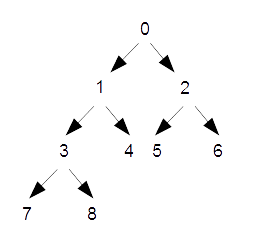
\includegraphics[scale=1]{figs/figure_heap.png}}
\caption{The heap corresponding to an array containing the digits 0 to 8}
\label{fig.heap}
\end{figure}

Here is one way to build a heap (in partial alphabetic order) 
from a list of unordered letters:

\begin{verbatim}
sub build-heap (@array, $index is copy) {
    my $index-val = @array[$index];
    while ($index) {
        my $parent = Int( ($index - 1) / 2);
        my $parent-val = @array[$parent];
        last if $parent-val lt $index-val;
        @array[$index] = $parent-val;
        $index = $parent;
    }
    @array[$index] = $index-val;
}

sub heapify (@array) {
    for @array.keys -> $i {
        build-heap @array, $i;
    }
}

my @input =  <m t f l s j p o b h v k n q g r i a d u e c>; 
heapify @input;
say @input;
\end{verbatim}

Note that the heap is built in place (there is no 
need for a second array). The resulting array is 
displayed as follows:
\begin{verbatim}
[a b g d c k j l f h e m n q p t r o i u s v]
\end{verbatim}

Is this a correct heap? It's difficult to say at first 
glance and checking it manually is somewhat tedious. When 
writing a program for building such a data structure, 
it is often useful to write some subroutines to display 
the content in a way that makes it easier to understand 
the result and check its correctness. The following 
code shows two examples of such possible subroutines:
\begin{verbatim}
sub print-heap (@array) {
    my $start = 0;
    my $end = 0;
    my $last = @array.end;
    my $step = 1;
    loop {
        say @array[$start..$end];
        last if $end == $last;
        $start += $step;
        $step *= 2;
        $end += $step;
        $end = $last if $end > $last;
    } 
}

sub print-heap2 (@array) {
    my $step = 0;
    for @array.keys -> $current {
        my $left_child = @array[2 * $current + 1];
        say "$current\tNode = @array[$current];\tNo child" 
             and next unless defined $left_child;
        my $right_child = @array[2 * $current + 2] // "' '";
        
        say "$current\tNode = @array[$current];\tChildren: " . 
             " $left_child and $right_child";
        $step++;
    }
}
\end{verbatim}

The first one displays the related tree level by level:

\begin{verbatim}
(a)
(b g)
(d c k j)
(l f h e m n q p)
(t r o i u s v)
\end{verbatim}

which makes it easy to draw the tree (see Figure~\ref{fig.heap2}).

\begin{figure}
\centerline
{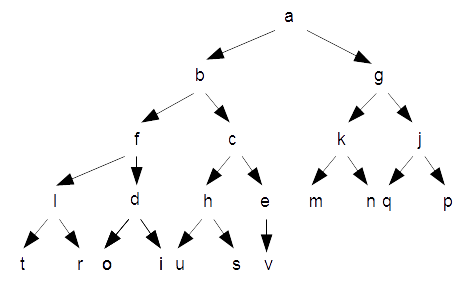
\includegraphics[scale=1]{figs/figure_heap2.png}}
\caption{The heap corresponding to the array of letters}
\label{fig.heap2}
\end{figure}


The second one shows the children for each node and makes it 
possible to easily check that the partial alphabetic order 
constraint is satisfied (i.e., each node is smaller than its 
children):

\begin{verbatim}
0       Node = a;       Children:  b and g
1       Node = b;       Children:  d and c
2       Node = g;       Children:  k and j
3       Node = d;       Children:  l and f
4       Node = c;       Children:  h and e
5       Node = k;       Children:  m and n
6       Node = j;       Children:  q and p
7       Node = l;       Children:  t and r
8       Node = f;       Children:  o and i
9       Node = h;       Children:  u and s
10      Node = e;       Children:  v and ' '
11      Node = m;       No child
12      Node = n;       No child
(...)
21      Node = v;       No child
\end{verbatim}



\section{Debugging}
\index{debugging}

When you are debugging a program, and especially if you are
working on a hard bug, here are some things to try:

\begin{description}

\item[Reading] Examine your code, read it back to yourself, and
check that it says what you meant to say.

\item[Running] Experiment by making changes and running different
versions.  Often if you display the right thing at the right place
in the program, the problem becomes obvious, but sometimes you have to
build scaffolding.

\item[Running under a debugger] A {\bf debugger} is a utility 
program that enables you to run a program step by step, 
so you can follow the execution path and check the content of important 
variables at crucial points in the program execution, to set 
break points, etc. Raku provides a debugger, called 
{\tt raku-debug}, that makes all these things possible. With the 
advent of modern high-level languages, many people balk at 
using a debugger. This is a mistake. A debugger will not help 
solve every kind of problem, but it can be immensely 
useful. See Section~\ref{raku-debugger} for more information
on the Raku debugger.
\index{debugger}

\item[Ruminating] Take some time to think!  What kind of error
is it: syntax, runtime, or semantic?  What information can you get from
the error messages, or from the output of the program?  What kind of
error could cause the problem you're seeing?  What did you change
last, before the problem appeared?

\item[Rubber ducking] If you explain the problem to someone else, you
sometimes find the answer before you finish asking the question.
Often you don't need the other person; you could just talk to a rubber
duck.  That's the origin of the well-known strategy called {\bf
rubber duck debugging}.  I am not making this up; see 
\url{https://en.wikipedia.org/wiki/Rubber_duck_debugging}.
\index{rubber duck debugging}

\item[Retreating] At some point, the best thing to do is back
off, undoing recent changes, until you get back to a program that
works and that you understand.  Then you can start rebuilding.

\end{description}

Beginning programmers sometimes get stuck on one of these activities
and forget the others.  Each activity comes with its own failure
mode.
\index{typographical error}

For example, reading your code might help if the problem is a
typographical error, but not if the problem is a conceptual
misunderstanding.  If you don't understand what your program does, you
can read it 100 times and never see the error, because the error is in
your head.
\index{experimental debugging}

Running experiments can help, especially if you run small, simple
tests.  But if you run experiments without thinking or reading your
code, you might fall into a pattern we call ``random walk programming,'' 
which is the process of making random changes until the program
does the right thing.  Needless to say, random walk programming
can take a very long time.
\index{random walk programming}
\index{development plan!random walk programming}

You have to take time to think.  Debugging is like an
experimental science.  You should have at least one hypothesis about
what the problem is.  If there are two or more possibilities, try to
think of a test that would eliminate one of them.

But even the best debugging techniques will fail if there are too many
errors, or if the code you are trying to fix is too big and
complicated.  Sometimes the best option is to retreat, simplifying the
program until you get to something that works and that you
understand.

Beginning programmers are often reluctant to retreat because
they can't stand to delete a line of code (even if it's wrong).
If it makes you feel better, copy your program into another file
before you start stripping it down.  Then you can copy the pieces
back one at a time.

Finding a hard bug requires reading, running (with or without 
a debugger), ruminating, and sometimes retreating.  If you get 
stuck on one of these activities, try the others.


\section{Glossary}

\begin{description}

\item[Deterministic] Pertaining to a program that does the same
thing each time it runs, given the same inputs.
\index{deterministic}

\item[Pseudorandom] Pertaining to a sequence of numbers that appears
to be random, but is generated by a deterministic program.
\index{pseudorandom}

\item[Default value] The value given to an optional parameter if no
argument is provided.
\index{default value}

\item[Override] To replace a default value with an argument.
\index{override}

\item[Benchmarking] The process of choosing between various data 
structures and algorithms by implementing alternatives and testing 
them (especially their run durations) on a sample of the possible inputs.  
\index{benchmarking}

\item[Debugger] A program that lets you run your code line by 
line and check its state at any step during its execution.
\index{debugger}

\item[Rubber duck debugging] Debugging by explaining your problem
to an inanimate object such as a rubber duck.  Articulating the
problem can help you solve it, even if the rubber duck 
doesn't know Raku. 
\index{rubber duck debugging}
\index{debugging!rubber duck}

\end{description}



\section{Exercises: Huffman Coding}
\label{huffman_exercise}

Huffman coding is a technique used for data compression, i.e., 
to reduce the size of a piece of data (such as, for example, 
compressing a file).

\subsection{Variable-Length Codes}
\index{variable-length code}

If you are familiar with Morse code, you know that it is a 
system for encoding the letters of the alphabet as a series 
of dots and dashes. For example, the famous signal {\tt ...---...} 
represents the letters SOS, which comprise an 
internationally recognized call for help. The table 
in Figure~\ref{fig.morse} shows the rest of the codes.
\index{Morse code}

\begin{figure}
\centerline
{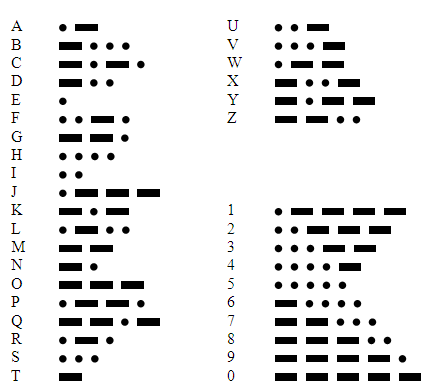
\includegraphics[scale=0.6]{figs/International_Morse_Code.PNG}}
\caption{International Morse code (public domain)}
\label{fig.morse}
\end{figure}

Morse code (invented between 1836 and 1844) was one of the 
very first attempts at digital encoding of the alphabet of a 
plain text. The only known earlier attempt is the braille 
alphabet (1824-1837).
\index{Morse, Samuel}
\index{braille alphabet}

Notice that some codes are longer than others. By design, the 
most common letters have the shortest codes. Since there are a 
limited number of short codes, that means that less common letters 
and symbols have longer codes. A typical message will have more 
short codes than long ones, which minimizes the average 
transmission time per letter.

Codes like this are called variable-length codes. In this exercise, 
we will look at an algorithm for generating a variable-length code 
called a Huffman code. It is an interesting algorithm in its own 
right, but it also makes a useful exercise because its implementation 
uses a variety of data structures.
\index{Huffman!code}

Here is an outline of what we will do until the end of this 
chapter:

\begin{enumerate}

\item First, we will use a sample of English text to generate 
a table of characters and their frequencies.

\item Then we will use this frequency table to generate a code 
table.

\item Finally, we will encode a message with this code table 
and then decode it.

\end{enumerate}

\subsection{The Frequency Table}
\index{frequency!table}

Since the goal is to give short codes to common letters, we 
have to know how often each letter occurs. In Edgar Allan Poe’s 
short story ``The Gold Bug,'' one of the characters, William~Legrand, 
uses letter frequencies to crack a cypher. He explains:
\index{Poe, Edgar Allan}
\index{The Gold-Bug (Edgar Allan Poe)}
\index{cypher}

\begin{quote}
``Now, in English, the letter which most frequently occurs 
is e. Afterwards, the succession runs thus: a o i d h n r s 
t u y c f g l m w b k p q x z. E however predominates so 
remarkably that an individual sentence of any length is 
rarely seen, in which it is not the prevailing character.''
\end{quote}

So our first mission is to see whether Poe got it right. 
To check, let's use as a sample the text of ``The Gold Bug'' 
itself, which can be downloaded from Project Gutenberg 
(\url{http://www.gutenberg.org/files/2147/2147-0.txt}) and 
a variety of other websites. 
\index{Project Gutenberg}

\begin{exercise}
\label{letter_frequency}
Write a program that counts the number of times each letter 
appears in a sample text. Download the text of ``The Gold Bug'' 
and analyze the frequency of the letters.

Solution: see Section~\ref{sol_letter_frequency}
\end{exercise}

\subsection{Building the Huffman Code}
\index{Huffman!code}

For our purposes, Morse code has one defect: it does not 
use just two symbols as you might think, but actually three: 
in addition to the dots and dashes, it it also implicitly 
using the space between two symbols, as well as a longer space 
between two letters.
\index{Morse code}

The reason why some space is needed is quite simple. Refer to the Morse 
code table above and suppose you receive three dots (\verb'...'). 
This could be interpreted as the letter ``e'' three times , or as 
``ie'' or ``ei,'' or as ``s'', or as the beginning of ``h,'' ``v,'' 
``3,'' ``4,'' or ``5''. Added spaces make it possible to disambiguate 
between those various possibilities. But they also make code 
transmission much slower.

In 1951, David A. Huffman invented a code-building technique avoiding 
this problem: provided that you know where a given letter starts, 
it is totally unambiguous. For example, we will meet later a Huffman 
code for a small subset of the alphabet that looks like this:
\index{Huffman, David A.}
\index{Huffman!code}

\begin{verbatim}
a => ..
e => .-
s => -.-
n => -..
t => --.
d => ---.
r => ----
\end{verbatim}

If you start reading a sequence of dots and dashes representing a 
valid text composed with these seven letters, you can always decode 
it without any ambiguity. If the first symbol is a dot, then the letter 
is either an ``a'' or a ``e'' depending on the next symbol. If the 
first symbol is a dash and the next one a dot, then the letter must 
be either a ``s'' or an ``n'' depending on the third symbol. If the 
two first symbols are dashes, you can similarly determine that the 
current letter is a ``t'' (if the third symbol is a dot), or a ``d'' 
or a ``r,'' which you can find out by looking at the fourth symbol. 
In brief, you don't need spaces between the symbols, it is always 
possible to unambiguously decode a letter.

How can we build such a Huffman code? Let's do it by hand with a 
very simple alphabet: the four letters of the nucleo-bases of DNA: A, 
C, T, and G. Suppose we want to encode the following input string:
\index{DNA (deoxyribonucleic acid)}
\index{alphabet}

\begin{verbatim}
CCTATCCTCGACTCCAGTCCA
\end{verbatim}

This gives the following frequency table:
\index{frequency!table}

\begin{verbatim}
C :     10      47.62
T :     5       23.81
A :     4       19.05
G :     2        9.52
\end{verbatim}

To build the Huffman code, we start with the two less frequent 
letters and merge them into one new temporary symbol, \verb"[GA]", 
which we pretend is a new composite letter with a 
frequency of 6. At this point, we decide that, between two letters, 
the less frequent one will have an appended dot and the other 
an appended dash (this is an arbitrary choice, it could be done 
the other way around). So we say that the symbol for the least 
common of the two letters (``G'') will be \verb'[GA].' and the 
symbol for ``A'' will be \verb'[GA]-'. 

We are now left with three letters, C, T, and [GA]. We merge the 
two least frequent letters, ``T'' and ``[GA],'' and can now tell 
that the symbol for ``T'' will be \verb'[TGA].' and the symbol for 
\verb'[GA]' will be \verb'[TGA]-'. There are only two letters left, 
``C'' and ``TGA'', with ``C'' the least frequent one; so ``C'' will
be a dot and ``TGA'' a dash.

We can now unroll our dummy letters: ``T'' is \verb'[TGA].', so, 
replacing \verb'[TGA]' with its symbol, i.e., a dash, the 
final code for ``T'' will be \verb'-.'; similarly, \verb'[GA].' 
now translates into \verb'--'. By the same substitution process, 
we can now determine that ``A'' is \verb'---' and ``G'' 
\verb'--.'. So our final Huffman code table is:
\index{Huffman!table}

\begin{verbatim}
C => .
T => -.
G => --.
A => ---
\end{verbatim}

Notice that, by construction, the most frequent letter (C) 
has the shortest code and the least common letters (G and A) 
the longest codes.

Manually encoding the \verb'CCTATCCTCGACTCCAGTCCA' input string 
with this code yields the following pseudo-Morse code:
\index{pseudo-Morse}

\begin{verbatim}
..-.----...-..--.---.-...-----.-...---
\end{verbatim}

Note that our Huffman code is not ambiguous: the first dot can 
only be a ``C,'' and the second one also. The next symbol is a 
dash, which can be the beginning of the three other letters, but 
only ``T'' can have a dot afterwards. The next sequence of 
symbols is four dashes; this can only be the three dashes of a 
``A'', with the last dash being the beginning of the next letter; 
and \verb'-.' can only be a ``T,'' and so on.
\index{Huffman!code}

In a real-life Huffman encoding for text file compression, 
we would not use dots and dashes, but 0 and 1 bits; however,  
dots and dashes are just another nice way of representing 
those binary values. So, let's just pretend that dots and dashes 
are really 0 and 1 binary numbers.
\index{binary number}
\index{bit}

\index{data compression}
Did we really achieve data compression? Our pseudo-Morse string has 
38~binary symbols. The original input string had 21 characters 
or bytes, that is 168 bits. The data has been compressed by a 
factor of about 4.4. 
\index{byte}

Is Huffman coding better than a fixed-length code? A string 
representation where each letter would be represented by two 
bits (two bits can represent four letters) would require 
42~symbols. So, yes, we did obtain a better data compression 
than a fixed-length encoding (by about 10\%). This may seem 
to be a small achievement, but this is actually quite good with 
such a small alphabet. With real text data, Huffman coding can 
achieve significant data compression.


\begin{exercise}
\label{huffman_code_2}
\begin{enumerate}
\item Write a program that performs Huffman encoding of a simple string 
of characters. You may start with the DNA example above. Don't 
worry, though, if you don't get the same Huffman table as the one 
above: there can be more than one Huffman code for a given input 
string; but check that you obtain an unambiguous code. 
\index{Huffman!code}
\item Try it with strings having a larger alphabet (you'll probably 
want to start with a relatively small alphabet, because it can 
otherwise be tedious to check the result by hand).
\item Write a subroutine to encode an input string into 
pseudo-Morse using the generated Huffman table.
\index{pseudo-Morse}
\index{alphabet}
\item Write a subroutine to decode the pseudo-Morse output 
you've just generated for the previous question.
\end{enumerate}
%
Solution: see Section~\ref{sol_huffman_code_2}.
\index{Huffman!code}
\end{exercise}




\part{Moving Forward}

% intro_part_2.tex -- Introduction to second part
%
% \chapter{Introduction to the Second part of this book}

Now that you have reached the end of the first part 
of this book, you should non longer be a pure beginner. 
By now, you should be able to go through the official 
Perl~6 documentation (\url{https://docs.perl6.org}) 
and find your way. 

There are many more things to say about programming. 
The next three chapters will be devoted to more 
advanced concepts and new programming paradigms, including:
\begin{description}

\item[Object-oriented programming] We will describe how 
we can construct our own types and methods, which 
is a way to extend the language.

\item[Using grammars] This is a form of declarative 
programming in which you define axioms and rules 
and derive knowledge from these; grammars are a 
very powerful way to analyze textual content and 
are used to transform program source code into 
executable statements.

\item[Functional programming] This is yet another programming 
paradigm in which computation is expressed as the 
evaluation of mathematical functions.
\end{description}

Each of these chapters probably deserves a full 
book in its own right (and might have one some day), 
but we hope to tell you enough about them to get you 
going. In my opinion, every programmer should know 
about these powerful concepts in order to be able 
to select the best way to solve a given problem.

Perl~6 is a multiparadigm language, so we can 
really cover these topics in terms of the Perl~6 
language. A number of subjects that we have 
introduced in previous chapters should lead you 
easily into these new ideas, and this is the 
reason why I think it is possible to properly cover 
them with just one chapter for each of these subjects.

There will be far fewer exercises in the second part, 
because we expect you by now to be able to think up 
your own exercises and make your own experiments for 
yourself. And there will be only very few suggested solutions, 
because we are getting at a level where there is really not  
one right solution, but many possible ways to tackle 
a problem.

Concerning the Perl language, we have covered a lot of 
material, but, as we warned from the very beginning, 
this is far from exhaustive. The following are among 
the topics that we have not covered (and will not cover); 
you might want to explore the documentation on them 
yourself:

\begin{description}
\item[Concurrent programming] Today's computers have 
multiple processors or multicore processors; Perl~6 
offers various ways of taking advantage of these to 
run computing processes in parallel in order to 
improve performance and reduce run time; see 
\url{https://docs.perl6.org/language/concurrency} 
for more details.

\item[Exception handling] Managing situations where 
something goes wrong is an important part of 
programming. Perl~6 offers various mechanisms to 
handle such situations. See \url{https://docs.perl6.org/language/exceptions} 
for more details.

\item[Interprocess communication:] Programs often have to 
run other programs and to communicate with them. See 
\url{https://docs.perl6.org/language/ipc}.

\item[Modules] How to create, use, and distribute Perl~6 
modules. See \url{https://docs.perl6.org/language/modules}.

\item[Native calling interface] How to call libraries 
that are written in other programming languages and 
follow the C calling conventions. 
See \url{https://docs.perl6.org/language/nativecall}

\end{description}

\chapter{Classes and Objects}
\label{objects}
\index{object}
\index{class}


At this point you know how to use functions to organize code and 
built-in types to organize data.  The next step is to learn
``object-oriented programming,'' which uses programmer-defined types
to organize both code and data.

\index{abstraction}
\index{encapsulation}
When software applications start to grow large, the number of 
details to be handled becomes overwhelming. The only 
way to manage this complexity is to use abstraction and 
encapsulation. Object orientation is a very popular and efficient 
way to implement abstraction and encapsulation.

Raku is an {\bf object-oriented programming language}, which means
that it provides features that support object-oriented
programming, which has these defining characteristics:
\index{object-oriented programming}

\begin{itemize}

\item Programs include class and method definitions.
\index{class}
\index{method}

\item Most of the computation is expressed in terms of operations on
  objects.

\item Objects often represent things in the real world, and methods 
often correspond to the ways things in the real world interact.

\end{itemize}


Object-oriented programming in 
Raku is a big topic that may be worth a book by itself (and 
there will probably be a book or two on the subject at some point). 
This chapter will hopefully do more than just skim the surface 
and enable you to create and use objects, but will not 
cover some of the details and more advanced features.
\index{OOP (object-oriented programming)}
\index{object-oriented programming (OOP)}

\section{Objects, Methods and Object-Oriented Programming}
\index{object-oriented programming (OOP)}
\index{programming!object-oriented}

Let us start with a high-level nontechnical overview 
of object-oriented programming in general and a brief 
introduction to the jargon associated with it.

\index{object}
In computer science, an object may loosely describe a memory 
location or an entity having a value, and often be referred to 
by an identifier. This can be a variable, a data structure, 
an array, or possibly even a function. This general meaning 
is not the sense that we will use in this chapter.

In object-oriented programming (OOP), the word {\bf object} 
has a much more specific meaning: an object is an entity 
which often has:
\begin{itemize}

\item An identity (for example its name).

\index{object! behavior}
\item Some properties defining its behavior (in the form of 
special functions that are usually called {\bf methods}); this 
behavior usually does not change over time and is generally 
common to all objects of the same type.
\index{method}

\item A {\bf state} defined by some special variables (called, 
depending on the language, attributes, instance data, fields, 
or members); the state may change over time and is generally 
specific to each object. In Raku, we speak about 
{\bf attributes}.
\index{object!state}
\index{object!attribute}
\index{attribute!object}
\end{itemize}

In brief, an object is a set of attributes and methods packed 
together.

\index{class}
Objects are usually defined in a kind of code package called 
a {\bf class}. A class defines the methods and the nature of 
the attributes associated with an object. In Raku, a class makes it 
possible to define new types similar to the built-in types 
that we have seen before. Very soon, we will start to define 
some classes and to use them to create objects.
\index{type!building new type}

\index{invocant}
\index{method}
\index{dot notation}
You already know informally what a method is, as we have 
used built-in methods throughout the book. It is a sort of 
function with a special postfix syntax using the dot notation 
on the invocant. For example, you may invoke the {\tt say} 
method on a simple string:

\begin{verbatim}
"foo".say;           # -> foo
\end{verbatim}

Note that ``foo'' isn't an object, but a simple string, but 
you can invoke the \verb'say' method on it, because Raku 
can treat it internally as an object when needed. In some 
OOP languages, this implicit conversion of a native type 
into an object is sometimes called autoboxing.
\index{autoboxing}

You probably also remember that methods can be chained in a 
process where the value returned by a method becomes the 
invocant for the next method:

\begin{verbatim}
"foo".uc.say;        # -> FOO

my @alphabet = <charlie foxtrot alpha golf echo bravo delta>;
@alphabet.sort.uc.say;
    # prints: ALPHA BRAVO CHARLIE DELTA ECHO FOXTROT GOLF 
\end{verbatim}

\index{role}
In OOP, methods applicable to objects are usually defined 
within classes, often the class that also defined the 
object or some other class closely related to it. In Raku, 
methods can also be defined in a {\bf role}, which is 
another type of code package somewhat resembling to a class, 
as we will see later.

\index{black box}
\index{encapsulation}
The basic idea of object-oriented programming is that an 
object is a kind of black box that hides its internals
(data and code) from the user; the user can consult or change 
the state of an object through the methods. Hiding the 
internals of objects is called {\bf encapsulation}. This 
often enables a higher-level view and a better data 
abstraction than what we have seen so far; this in turns 
helps to make programs less buggy (especially large programs).

In addition, OOP usually also offers the following concepts:
\begin{itemize}
\index{polymorphism}
\item {\bf polymorphism}, i.e., the possibility for a function or 
a method to do different things depending of the type of 
object which calls it;
\index{inheritance}
\item {\bf inheritance}, i.e., the possibility to derive a class from 
another class, so that the child class inherits some of 
the properties of the {\bf parent class}, which is a powerful tool 
for code reuse.
\end{itemize}

We will now study how all these concepts are implemented in Raku.


\section{Programmer-Defined Types}
\label{point}
\index{programmer-defined type}
\index{type!programmer-defined}

We have used many of Raku's built-in types; now we are going
to define a new type.  As an example, we will create a type
called {\tt Point2D} that represents a point in 
two-dimensional space.
\index{point, mathematical}
\index{two-dimensional space}

In mathematical notation, points are often written in
parentheses with a comma separating the coordinates. For example,
in Cartesian or rectangular coordinates, $(0,0)$ represents 
the origin, and $(x,y)$ represents the point $x$ units to the 
right and $y$ units up from the origin. $x$ is called 
the abscissa of the point, and $y$ the ordinate.
\index{Cartesian coordinates}
\index{coordinates!Cartesian}
\index{coordinates!rectangular}
\index{rectangular coordinates}

There are several ways we might represent points in Raku:

\begin{itemize}

\item We could store the coordinates separately in two
variables, {\tt \$x} and {\tt \$y}.

\item We could store the coordinates as elements in a list, 
an array, or a pair.

\item We could create a new type to represent points as
objects.

\end{itemize}
\index{representation}

Creating a new type is a bit more complicated than the 
other options, but it has advantages that will be apparent soon.

A programmer-defined type is usually created by a {\bf class}
(or a \emph{role}, but we will come back to that later). 
A barebones class definition for a point type looks like this:
\index{class}
\index{object!class}
\index{class!definition}
\index{definition!class}
\index{role}
\index{Point2D class}

\begin{verbatim}
class Point2D {
    has $.abscissa;              # "x" value
    has $.ordinate;              # "y" value
}
\end{verbatim}
%
The header indicates that the new class is called {\tt Point2D}.
The body is defining two attributes, i.e., named properties 
associated with the class, here the abscissa and ordinate 
(or $x$ and $y$ coordinates) of the point.
\index{Point2D class}
\index{class!Point2D}

\index{type object}
Defining a class named {\tt Point2D} creates a {\bf type object}.

The type object is like a factory for creating objects.  To create 
a point, you call the {\tt new} method on the {\tt Point2D} class:

\begin{verbatim}
my $point = Point2D.new( 
    abscissa => 3, 
    ordinate => 4
);
say $point.WHAT;                # -> (Point2D)
say $point.isa(Point2D);        # -> True
say $point.abscissa;            # -> 3
\end{verbatim}
%
\index{isa method}
\index{WHAT}
You can of course create as many points as you wish.

\index{constructor}
\index{new, object constructor}
\index{dot notation}
\index{object!constructor}
The {\tt new} method is called a {\bf constructor} and has not 
been defined in this example; this is not needed because 
Raku supplies a default {\tt new} constructor method for 
every class (we'll see later how). The method invocation 
syntax, with the dot notation, is the same as what we have 
used throughout the book to invoke built-in methods. You 
are not forced to use this constructor; you can also create 
your own (and you may name it {\tt new} or something else), 
but we will stay with the built-in {\tt new} method for the 
time being.
\index{invocation!method}
\index{method invocation}

Creating a new object with a class is called {\bf instantiation}, 
and the object is an {\bf instance} of the class.
\index{instance}
\index{object!instance}
\index{instantiation}

Every object is an instance of some class, so the terms 
``object'' and ``instance'' are interchangeable.  But 
we will often use ``instance'' to indicate that we are 
talking about an object belonging to a programmer-defined type.
\index{type}
\index{programmer-defined type}

\section{Attributes}
\label{attributes}
\index{instance attribute}
\index{attribute!instance}
\index{dot notation}

The attributes that we have defined are properties associated 
with the {\tt Point2D} class, but they are specific to the 
instance of the class that has been created. They are 
instance attributes. If we create another {\tt Point2D} object, 
it will also have these attributes, but the values of 
these attributes are likely to be different. 

Figure~\ref{fig.point2d} shows the result of these assignments.
A state diagram that shows an object and its attributes is
called an {\bf object diagram}.
\index{state diagram}
\index{diagram!state}
\index{object diagram}
\index{diagram!object}

\begin{figure}
\centerline
{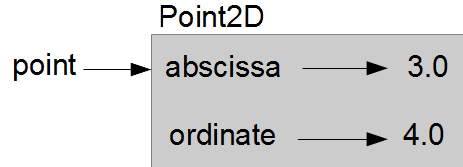
\includegraphics[scale=0.8]{figs/point2D.png}}
\caption{Object diagram.}
\label{fig.point2d}
\end{figure}

The variable {\tt \$point} refers to a {\tt Point2D} object, 
which contains two attributes.  

Each attribute of the {\tt Point2D} class should refer to a 
number, but this is not obvious in the current definition of 
the class. As it stands right now, we could create a {\tt Point2D} 
object with a string for the abscissa, which would not make 
much sense. We can improve the class definition by specifying 
a numeric type for the attributes:
%
\begin{verbatim}
class Point2D {
    has Numeric $.abscissa;              # "x" value
    has Numeric $.ordinate;              # "y" value
}
\end{verbatim}
%
\index{private attribute}
\index{attribute!private}
The instance attributes are private to the class, which means 
that they normally cannot be accessed from outside the class: 
you would usually need to invoke a method of the class 
(i.e., a kind of subroutine defined within the class), to get 
their value. However, when an attribute is defined with a dot 
as in \verb'$.abscissa':

\begin{verbatim}
    has $.abscissa;  
\end{verbatim}
%
\index{accessor}
\index{method!accessor}
Raku automatically creates an implicit \emph{accessor} method, 
i.e., a method having the same name as the attribute that returns 
the value of this attribute. Thus, when we wrote:

\begin{verbatim}
say $point.abscissa;                     # -> 3
\end{verbatim}
%
we were not accessing directly the {\tt abscissa} attribute of 
the \verb'$point' object, but we were really calling the 
{\tt abscissa} method on the object, which in turn returned 
the value of that attribute.

\index{dot notation}
\index{accessor}
You can use such an accessor with dot notation as part of any 
expression. For example:

\begin{verbatim}
my $dist-to-center = sqrt($point.abscissa ** 2 + $point.ordinate ** 2);
\end{verbatim}
%

There is another way to declare an attribute in a class, with 
an exclamation mark twigil instead of a dot:
\index{twigil}

\begin{verbatim}
    has $!abscissa;  
\end{verbatim}
%
\index{attribute!private}
\index{private attribute}
In that case, Raku does not create an implicit accessor method 
and the attribute can only be accessed from methods within 
the class. Such an attribute is now fully private. 
However, if you declare attributes this way, you 
will not be able to populate them at object creation with 
the default {\tt new} constructor and will need to create your 
own constructor (or indirectly modify {\tt new}). So don't try 
that for the time being, as you would not be able to do much 
with your objects at this point. We'll get back to that later.

\index{attribute!mutable}
\index{attribute!immutable}
By default, object attributes are not mutable; they are read-only. 
This means you cannot modify them once the object has been created. 
This is fine for some attributes: if an object represents a 
person, that person's name and birth date are unlikely to 
change. Some other attributes may need to be updated, sometimes 
very frequently. In such cases, attributes can be declared 
to be mutable with the {\tt is rw} trait:
\index{is rw trait}
\index{trait!is rw}

\begin{verbatim}
class Point2D {
    has Numeric $.abscissa is rw;              # "x" value
    has Numeric $.ordinate is rw;              # "y" value
}
\end{verbatim}
%
It is now possible to modify these attributes. For example, 
we can change the newly created point's abscissa:

\begin{verbatim}
# First creating a Point2D object:
my $point = Point2D.new(abscissa => 3, ordinate => 4);
say $point;    # -> Point2D.new(abscissa => 3, ordinate => 4)

# Now moving the $point object two units to the right:
$point.abscissa = 5; 
say $point;    # -> Point2D.new(abscissa => 5, ordinate => 4)
\end{verbatim}


\index{class!attribute}
\index{attribute!class}
Almost all of the information presented so far about attributes 
has been related to instance attributes, i.e., to properties related to 
individual objects. You can also have attributes pertaining 
to the whole class, which are named \emph{class attributes}. 
They are less common than instance attributes and are declared 
with the {\tt my} declarator (instead of {\tt has}). A typical 
example of a class attribute would be a counter at the class level 
to keep track of the number of objects that have been 
instantiated. 


\section{Creating Methods}
\index{method}

The simple {\tt Point2D} class and its instance \verb'$point' 
are not very useful so far. Let's complete the class definition 
with some methods:
\index{Point2D class}

\begin{verbatim}
class Point2D {
    has Numeric $.abscissa;
    has Numeric $.ordinate;
    
    method coordinates {        # accessor to both x and y
        return (self.abscissa, self.ordinate)
    }
    
    method distance2center {
        (self.abscissa ** 2 + self.ordinate ** 2) ** 0.5
    }
    method polar-coordinates {
        my $radius = self.distance2center;
        my $theta = atan2 self.ordinate, self.abscissa;
        return $radius, $theta;
    }
}
\end{verbatim}

We declare three methods in the class:
\begin{itemize}
\item {\tt coordinates}, a simple accessor to the Cartesian 
coordinates;
\index{coordinates!Cartesian}
\index{Cartesian coordinates}

\item{\tt distance2center}, a method to compute and return 
the distance between the object and the origin;

\index{polar coordinates}
\index{coordinates!polar}
\item{\tt polar-coordinates}, a method to compute the radius 
and azimuth (\verb'$theta') of the object in the polar 
coordinates system (notice that {\tt polar-coordinates} 
invokes the {\tt distance2center} method to find the radius 
component of the polar coordinates).
\end{itemize}

\index{invocant}
A method definition is not very different from a subroutine 
definition, except that it uses the {\tt method} keyword 
instead of the {\tt sub} keyword. This is not a surprise 
since a method is essentially a subroutine that is defined 
within a class (or a role) and knows about its 
\emph{invocant}, i.e., the object that called it and its class. 
And, of course, it has a different calling syntax.
\index{method}

\index{method!dispatch}
\index{dispatching methods}
\index{invocation!method}
\index{method invocation}
Another important difference between a subroutine and a method 
is that, since there may be several methods with the same name 
defined in different classes (or different roles), a method 
invocation involves a \emph{dispatch} phase, in 
which the object system selects which method to call, usually 
based on the class or type of the invocant. However, in 
Raku, that difference is blurred by the fact that you can 
have multi subroutines, i.e., subroutines with the same name 
and a different signature that are also resolved at run time, 
depending on the \emph{arity} (number of arguments) and type of 
the arguments. 
\index{arity}
\index{type}

Within a method definition, {\tt self} refers to the 
\emph{invocant}, the object that invoked the method. 
There is a short hand for it, \verb'$.', so that we could 
write the {\tt coordinates} method as follows:
\index{self}

\begin{verbatim}
    method coordinates {        # accessor to both x and y
        return ($.abscissa, $.ordinate)
    }
\end{verbatim}

The two  syntax formats, \verb'$.' and {\tt self}, are 
essentially equivalent.

There is a third syntactic way of doing it, using an 
exclamation mark instead of a dot:

\begin{verbatim}
    method coordinates {        # accessor to both x and y
        return ($!abscissa, $!ordinate)
    }
\end{verbatim}

Here, the result would be the same, but this new syntax is 
not equivalent: \verb'$.abscissa' is a method invocation, 
whereas \verb'$!abscissa' provides direct access to the attribute.
The difference is that \verb'$!abscissa' is available only 
within the class (and might be slightly faster), while 
the method invocation syntax can be used somewhere else 
(for example in another class). We will see in the next section 
examples of this distinction and its consequences.
\index{invocation!method}
\index{method invocation}

We can now create an object and call our methods on it:

\begin{verbatim}
my $point =  Point2D.new(
    abscissa => 4, 
    ordinate => 3
);
say $point.coordinates;         # -> (4 3)
say $point.distance2center;    # -> 5
say $point.polar-coordinates;    # -> (5 0.643501108793284)
\end{verbatim}

\index{topical variable}
\index{invocant}
You might remember from previous chapters that if you use a method 
without naming an explicit invocant, then the method applies to 
the \verb'$_' topical variable:

\begin{verbatim}
.say for <one two three>;       # -> one two three (each on one line)
\end{verbatim}

\index{for loop}
\index{given statement}
Now that we have created an object with some methods, we can also 
take advantage of the same syntax shortcut. For example if we 
use {\tt for} or {\tt given} to populate the \verb'$_' topical 
variable with the \verb'$point' object, we can write:

\begin{verbatim}
given $point {
    say .coordinates;          # -> (4 3)                       
    say .distance2center;     # -> 5                 
    .polar-coordinates.say;     # -> (5 0.643501108793284)
}    
\end{verbatim}

As an exercise, you could write a method called 
\verb"distance_between_points" that takes two points 
as arguments and returns the distance between
them using the Pythagorean theorem.

The methods of our class so far are all \emph{accessors}, which 
means they provide a snapshot of some of the invocant's attributes. 
If the attributes are mutable (declared with the \verb'is rw' 
trait), we can also create some \emph{mutators}, i.e., methods 
that can be invoked to change those mutable attributes:
\index{accessor}
\index{mutator}

\begin{verbatim}
class Point2D-mutable {
    has Numeric $.abscissa is rw;
    has Numeric $.ordinate is rw;
    
    # perhaps the same accessors as in the class definition above
    
    method new-ordinate (Numeric $ord) {
        self.ordinate = $ord; 
    }
}
# Creating the Point2D-mutable object:
my $point = Point2D-mutable.new(abscissa => 3, ordinate => 4);
say $point;  # -> Point2D-mutable.new(abscissa => 3, ordinate => 4)

# Modifying the ordinate:
$point.new-ordinate(6);
say $point;  # -> Point2D-mutable.new(abscissa => 3, ordinate => 6)
\end{verbatim}




\section{Rectangles and Object Composition}
\label{rectangles}
\index{rectangle}
\index{composition!object}
\index{object!composition}

Sometimes it is obvious what the attributes of an object should be,
but other times you have to make decisions.  For example, imagine you
are designing a class to represent rectangles.  What attributes would
you use to specify the location and size of a rectangle?  You can
ignore angle; to keep things simple, assume that the rectangle's edges 
are either vertical or horizontal.
\index{representation}

There are at least two possibilities: 

\begin{itemize}

\item You could specify one corner of the rectangle
(or the center), the width, and the height.

\item You could specify two opposing corners.

\end{itemize}

At this point it is hard to say whether either is better than
the other, so we'll implement the first one, just as an example.
\index{Rectangle class}
\index{class!Rectangle}

Here is the class definition:

\begin{verbatim}
class Rectangle {
    has Numeric $.width;
    has Numeric $.height;
    has Point2D $.corner;     # lower left vertex 

    method area { return $.width * $.height }
    method top-left { $.corner.abscissa, $.corner.ordinate + $.height; }
    # other methods, e.g. for other corners' coordinates, center, etc.
}
\end{verbatim}
%
The new feature compared to the previous {\tt Point2D} class 
definition is that the \verb'Rectangle' class can now use the 
{\tt Point2D} type created previously for defining the corner 
attribute. 

The {\tt top-left} method returns the coordinates of 
the top left angle of the rectangle. This {\tt top-left} 
method gives us an opportunity to explain a bit more 
the difference between the \verb'$.' and \verb'$!' twigils. We have 
used \verb'$.corner.abscissa' to obtain the abscissa of 
the corner, i.e., in effect an accessor invocation. We could 
have directly accessed the {\tt corner} and {\tt height} 
attributes of the {\tt Rectangle} class and used the following 
method definition:
\index{twigil}
\index{invocation!method}
\index{method invocation}

\begin{verbatim}
    method top-left { $!corner.abscissa, $!corner.ordinate + $!height; }
\end{verbatim}

But it would not be possible to use \verb'$!corner!abscissa' or 
\verb'$.corner!abscissa', because {\tt abscissa} is not an 
attribute defined in the {\tt Rectangle} class, and thus cannot 
be accessed directly there. You can use direct access 
to the attribute (for example with the \verb'$!abscissa' syntax) 
only within the class where this attribute is defined, 
{\tt Point2D}. So, in {\tt Rectangle}, we need to invoke the 
accessor (i.e., the syntax with \verb'$.') for obtaining the 
value of the corner abscissa.

We can now create a {\tt Rectangle} object:
\index{rectangle}

\begin{verbatim}
my $start-pt =  Point2D.new(abscissa => 4, ordinate => 3);
my $rect = Rectangle.new(corner => $start-pt, height => 10, width => 5);

say "top-left coord.: ", $rect.top-left;   # -> top-left coord.: (4 13)
say "Rectangle area: ", $rect.area;      # -> Rectangle area: 50
\end{verbatim}

\index{named parameter}
\index{parameter!named}
You might have noticed that the arguments passed to the 
{\tt Rectangle.new} constructor are not in the same order as 
in the class definition. I did that on purpose 
to show that the order is unimportant because we 
are using named arguments.

Figure~\ref{fig.rectangle} shows the state of this object.

\begin{figure}
\centerline
{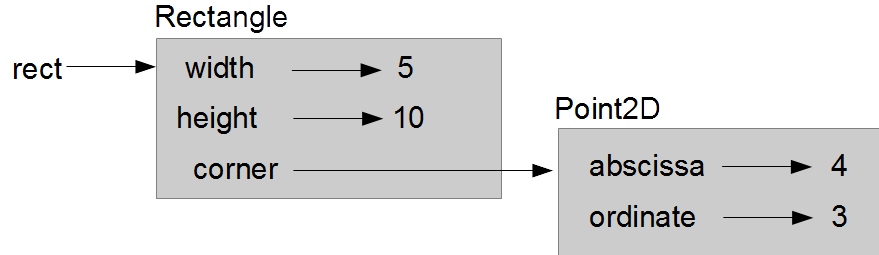
\includegraphics[scale=0.8]{figs/rectangle.png}}
\caption{Object diagram.}
\label{fig.rectangle}
\end{figure}

\index{state diagram}
\index{diagram!state}
\index{object diagram}
\index{diagram!object}
\index{embedded object}
\index{object!embedded}
\index{object!composition}
\index{composition!object}

Using an object as an attribute of another object, possibly 
of another class, is called {\bf object composition}. An object 
that is an attribute of another object is {\bf embedded}. Object 
composition makes it possible to easily define nested layers of 
abstraction and is a powerful feature of object-oriented 
programming. In our ``geometry'' example, we started to define 
a low-level object, a {\tt Point2D} instance, and then used 
that point to build a higher level type, {\tt Rectangle}.


\section{Instances as Return Values}
\index{instance!as return value}
\index{return!value}

Methods can return instances of another class.  For example, 
the {\tt Rectangle} class can have methods returning 
instances of {\tt Point2D} for the other corners:

\begin{verbatim}
    method top-right-point {
        return Point2D.new(
            abscissa => $!corner.abscissa + $!width, 
            ordinate => $!corner.ordinate + $!height
        );
    }
   # other methods for other corners
\end{verbatim}

Notice that we don't even bother to give a name to upper right 
point (although we could, if we wanted); we create it with the 
constructor and return it on the fly.

We can use the new method as follows:

\begin{verbatim}
my $topRightPt = $rect.top-right-point;
say "Top right corner: ", $topRightPt;
# -> Top right corner: Point2D.new(abscissa => 9, ordinate => 13)
\end{verbatim}

\index{type}
Although this is not very useful in such a simple case, we 
could play it safe and declare a {\tt Point2D} type for 
\verb'$topRightPt':

\begin{verbatim}
my Point2D $topRightPt = $rect.top-right-point;
\end{verbatim} 

This way, the code will raise an error if the {\tt top-right-point} 
happens to return something other than a {\tt Point2D} instance.

Similarly, the \verb"find-center" method invoked on a 
{\tt Rectangle} returns a {\tt Point2D} instance 
representing the center of the {\tt Rectangle}:

\begin{verbatim}
    method find-center { Point2D.new(
            abscissa => $!corner.abscissa + $!width / 2, 
            ordinate => $!corner.ordinate + $!height / 2
        );
    }
\end{verbatim}
%
This new method can be used as follows:

\begin{verbatim}
say "Center = ", $rect.find-center;
# -> Center = Point2D.new(abscissa => 6.5, ordinate => 8.0)
\end{verbatim}
%

\section{Inheritance}
\index{inheritance}
\index{inheritance!class}
\index{class!inheritance}


Inheritance is probably the most emblematic feature of 
object-oriented programming. It is a mechanism through which it 
is possible to derive a class from another class. Inheritance is 
one of the standard ways to implement code reuse in 
object-oriented programming. It is also another useful way of 
defining successive layers of abstraction and a hierarchy of 
types.

\subsection{The Pixel Class}
\index{class!Pixel}
\index{Pixel class}

The {\tt Point2D} class is very general and could be used for 
a variety of purposes: geometry, vector graphics, animated mangas, 
and so on. We may want to use it to display graphic data on a 
screen. For this scenario, let's create a new derived class, 
{\tt Pixel}, adding new properties to the point, such as color, 
perhaps transparency, etc. 

Do we need to redefine all the attributes and methods for 
the new class? No, we don't. We can define a new class that 
\emph{inherits} the properties of the {\tt Point2D} base class 
and only modify what is no longer suitable or add whatever 
new features we need. Here, we want a new attribute to represent 
the pixel color and probably some new methods dealing with this 
new attribute.

According to the most common standards, a color is defined 
by three integers (really three octets, i.e., integers 
between 0 and 255 in decimal notation), representing the red, 
green, and blue (RGB) components of the pixel:
\index{class!child}
\index{Pixel class}
\index{RGB}
\index{octet}

\begin{verbatim}
class Pixel is Point2D {
    has %.color is rw;

    method change_color(%hue) {
        self.color = %hue
    }
    method change_color2(Int $red, Int $green, Int $blue) {
        # signature using positional parameters
        self.color = (red => $red, green => $green, blue => $blue)
    }
}
\end{verbatim}

\index{parameter!positional}
\index{parameter!named}
\index{positional parameter}
\index{octet}
\index{is!subclassing trait}
The new class \emph{inherits} the properties of {\tt Point2D} 
thanks to the {\tt is Point2D} trait, except possibly those 
that are explicitly modified (or overridden) or added in 
the new class. The new class is sometimes called a 
child class or subclass, whereas {\tt Point2D} is the 
parent class. Creating this new class based on 
{\tt Point2D} is called {\bf subclassing} the {\tt Point2D} 
parent class. 
\index{class!parent}
\index{class!child}
\index{class!subclass}
\index{subclassing}
\index{overriding a method}
\index{method!overriding}

The new child class inherits the {\tt abscissa} and 
{\tt ordinate} attributes of the {\tt Point2D} parent 
class (and their specific type and properties if any), 
as well as the methods such as {\tt coordinates} defined 
in the parent class. The child class  has a new 
attribute (the color) and two new methods.

Instantiating a {\tt Pixel} object is just about as easy as 
before, we only need to add an additional attribute parameter 
in the call to the {\tt new} constructor:

\begin{verbatim}
my $pix = Pixel.new(
    :abscissa(3.3),
    :ordinate(4.2),
    color => {red => 34, green => 233, blue => 145}, 
    );
say "The original pixel has the following colors: ", $pix.color;
\end{verbatim}

In the {\tt Pixel} class definition, we have written 
two different methods for changing the color 
only to illustrate two possible syntax formats, for pedagogical 
purposes. The first one receives a hash as a parameter, and 
the second one uses positional parameters, which forces 
the user to remember the order (RGB) in which the arguments must 
be passed; this can be a source of error and should be avoided 
when the number of parameters exceeds a certain limit 
(which will be left up to the reader). On the other 
hand, anyone working commonly with graphics knows by heart the 
standard conventional order of colors (i.e., RGB). Also, 
the second method has the 
advantage of enabling some type checks (the arguments must 
be integers). This is a simplified example; in real life, it 
may be desirable to check that the parameters are octets, i.e., 
integers between 0 and 255 (which could be done by adding a 
type constraint or defining a subset of the integer type).
\index{subset}
\index{RGB}
\index{octet}

Using the new {\tt Pixel} class is straight forward:

\begin{verbatim}
say "Original colors: ", $pix.color;

$pix.change_color({:red(195), :green(110), :blue(70),});
say "Modified colors: ", $pix.color;
say "New pixel caracteristics:";
printf "\tAbscissa: %.2f\n\tOrdinate: %.2f\n\tColors: R: %d, G: %d, B: %d\n",
       $pix.abscissa, $pix.ordinate, 
       $pix.color<red>, $pix.color{"green"}, $pix.color{"blue"};

$pix.change_color2(90, 180, 30);  # positional args
say "New colors:  
\tR: {$pix.color<red>}, G: {$pix.color<green>}, B: {$pix.color<blue>} ";
\end{verbatim}

This displays the following output:

\begin{verbatim}
Original colors: {blue => 145, green => 233, red => 34}
Modified colors: {blue => 70, green => 110, red => 195}
New pixel caracteristics:
        Abscissa: 3.30
        Ordinate: 4.20
        Colors: R: 195, G: 110, B: 70
New colors:  
        R: 90, G: 180, B: 30
\end{verbatim}

To tell the truth, it was not necessary to use two different 
method names, \verb'change_color' and \verb'change_color2', as 
we did in the {\tt Pixel} class definition to simplify matters. 
It would work the same way if we use these definitions:
\index{Pixel class}
\index{method dispatch}

\begin{verbatim}
    multi method change_color(%hue) {
        self.color = %hue
    }
    multi method change_color(Int $red, Int $green, Int $blue) {
        # signature using positional parameters
        self.color = (red => $red, green => $green, blue => $blue)
    }
\end{verbatim} 

Since the multi method is defined twice, with the same name but 
with a different signature, the object system is able to 
dispatch the invocation to the right method.
\index{method!dispatch}
\index{multi method}


\subsection{The MovablePoint Class}
\index{class!MovablePoint}
\index{MovablePoint class}

The \verb'$.abscissa' and \verb'$.ordinate' attributes of 
class {\tt Point2D} are defaulted to read-only. After all, 
when you define a point in the plan, it usually has a fixed 
position and there is generally no reason to change its 
coordinates.

Suppose, however, that our application is about kinematics 
(the branch of physics dealing with the motion of points or 
bodies) or is a video game. In such a case, we probably want 
our points (or sets of points) to move. We need a new class, 
{\tt MovablePoint}, enabling the modification of coordinates.

We don't need to redefine all the attributes and methods for 
the new class. Again, we can define a new class that 
\emph{inherits} the properties of the {\tt Point2D} base class 
and only modifies what is no longer suitable or adds whatever 
new features we need, for example:

\begin{verbatim}
class MovablePoint is Point2D {
    has Numeric $.abscissa is rw;
    has Numeric $.ordinate is rw;
    
    method move (Numeric $x, Numeric $y) {
        $.abscissa += $x;
        $.ordinate += $y;
    }
}
\end{verbatim}

\index{is!subclassing trait}
The new class inherits the properties of {\tt Point2D} thanks 
to the {\tt is Point2D} trait, except those that are explicitly 
modified (or overridden) or added in the new class. 
Methods that exist in the parent class and are 
redefined in a child class are said to be \emph{overridden} 
within that class. 
\index{class!parent}
\index{class!child}
\index{class!subclass}
\index{subclassing}
\index{overriding a method}
\index{method!overriding}

Here, the \verb'$.abscissa' and \verb'$.ordinate' attributes are 
redefined as read and write (through the {\tt is rw} trait) and 
a new method, {\tt move}, is defined to modify the position of 
a point by adding the received parameters to the coordinates 
of the point.
\index{is rw trait}

Note that we have used positional parameters here for the 
{\tt move} method. We said that it is often better for the sake of clarity 
to use named parameters, but we have only two parameters here; 
as it is fairly simple to remember that the \verb'$x' 
parameter should come before the \verb'$y' parameter, this 
was a good occasion to illustrate the possibility of using 
positional parameters.
\index{positional parameter}
\index{parameter!positional}
\index{parameter!named}
\index{named parameter}

We can now test our new child class, create a {\tt MovablePoint} 
instance, display its characteristics, move it to a different 
location, and display the new position:

\begin{verbatim}
my $point = MovablePoint.new(
    abscissa => 6,
    ordinate => 7,
    );

say "Coordinates : ", $point.coordinates;
say "Distance to origin: ", $point.distance2center.round(0.01);
printf "%s: radius = %.4f, theta (rad) = %.4f\n", 
    "Polar coordinates", $point.polar-coordinates;

say "--> Moving the point.";
$point.move(4, 5);
say "New coordinates: ", $point.coordinates;
say "Distance to origin: ", $point.distance2center.round(0.01);
printf "%s: radius = %.4f, theta (rad) = %.4f\n", 
    "Polar coordinates", $point.polar-coordinates;
\end{verbatim}

This produces the following output:

\begin{verbatim}
Coordinates : (6 7)
Distance to origin: 9.22
Polar coordinates: radius = 9.2195, theta (rad) = 0.8622
--> Moving the point.
New coordinates: (10 12)
Distance to origin: 15.62
Polar coordinates: radius = 15.6205, theta (rad) = 0.8761
\end{verbatim}

\index{polar coordinates}
\index{coordinates!polar}
Here, when the user code invokes the {\tt coordinates}, 
{\tt distance2center}, and {\tt polar-coordinates} methods, 
Raku finds that they do not exist in {\tt MovablePoint}. But,  
as \verb'MovablePoint' subclasses {\tt Point2D}, the program 
looks for methods having these names in the parent class and 
invokes them if it finds them. 	If it did not find them, it 
might look into the parent's parent to see if there are any, and 
so on.


\subsection{Multiple Inheritance: Attractive, but Is It Wise?}

In object-oriented programming, the inheritance mechanism is 
a traditional way to reuse code, it is even probably the most 
common way to do it. 

A class may have several parent classes and, thus, subclass 
several other classes. This is what is called {\bf multiple 
inheritance}. We might want to build a new {\tt MovablePixel} 
class inheriting from both {\tt MovablePoint} and {\tt Pixel} 
(and, indirectly, from {\tt Point2D}). Technically, you can 
easily do it in Raku:

\begin{verbatim}
class MovablePixel is MovablePoint is Pixel {
    # ...
}
\end{verbatim}

Now, {\tt MovablePixel} is subclassing both 
{\tt MovablePoint} and {\tt Pixel} and inheriting 
from both parent classes.
\index{subclass}
\index{class!parent}

This looks very promising, but it turns out to be more 
complicated than expected in real situations. If there is a 
conflict (for example a name collision between two methods), 
which one shall prevail? Some mechanisms exist to 
handle such situations (for example in the C++ programming 
language), and Raku has some metaobject methods to find out 
about the method resolution order (MRO), but this 
might quickly leads to severe design 
problems and to really subtle or complicated bugs. In 
short, while multiple inheritance originally looked as a 
attractive idea, it turned out to be complicated to master, 
because it creates multiple and often implicit dependencies 
that are quite hard to sort out.

This is the reason why, contrary to C++, relatively more recent 
OO programming languages such as Java (which came out not 
so recently, back in 1995) have decided not to implement 
multiple inheritance.

Raku does not want to forbid such things and allows you 
to use multiple inheritance if you wish, and it can be useful 
for simple cases; so don't necessarily rule it out, but 
remember that, contrary to early expectations, it often 
leads to a mess and turns out to be quite unmanageable.

Raku offers better concepts for tackling such situations,
as we will see shortly.

\section{Roles and Composition}
\index{role}
\index{inheritance}

Inheritance is a very powerful concept to describe a hierarchical 
tree of concepts. For example, you can think of a hierarchy of 
geometrical figures having more and more specific properties: 
\begin{enumerate}
\item Polygon

\index{quadrilateral}
\item Quadrilateral (a polygon with four edges and four corners)

\index{trapezoid}
\item Trapezoid (a quadrilateral with one pair of parallel edges)

\index{parallelogram}
\item Parallelogram (a trapezoid with two pairs of parallel 
edges and opposite sides of equal length)

\index{rectangle}
\item Rectangle (a parallelogram with four right angles)

\index{square}
\item Square (a rectangle with all four edges of equal length)
\end{enumerate}

\index{rhombus}
It is relatively easy to imagine a series of classes with a 
hierarchical inheritance tree reflecting those properties. It 
gets slightly more complicated, however, if we add the rhombus 
(a parallelogram with all sides equal), because the square is 
now \emph{also} a rhombus with four right angles. 
The square class would subclass both the rectangle and the 
rhombus, and we might have here a possible multiple inheritance 
issue.

\index{integer} \index{rational} \index{real number} \index{complex number}
\index{vertebrate} \index{mammal} \index{carnivoran}
\index{canid} \index{dog}
Similarly, we can think of a tree of classes with nested 
inheritance representing various types of numbers (e.g. integer, 
rational, real, complex) or animals species (e.g., vertebrate, 
mammal, carnivoran, canid, dog, Irish setter).

\index{hierarchical model}
These are great examples for inheritance, but the real world is 
rarely so hierarchical, and it is often difficult to force 
everything to fit into such a hierarchical model.

\index{role}
This is one of the reasons why Raku introduces the notion of 
roles. A role is a set of behaviors or actions that can be shared 
between various classes. Technically, a role is a collection 
of methods (with possibly some attributes); it is therefore 
quite similar to a class, but the first obvious difference 
is that a role is not designed to be instantiated as an object 
(although roles can be promoted into classes). The 
second difference, perhaps more important, is that roles 
don't inherit: they are used through application to a class 
and/or composition.

\subsection{Classes and Roles: An Example}

\index{vertebrate} \index{mammal} \index{dog}
Let's come back to vertebrates, mammals and dogs. A dog is 
a mammal and inherits some characteristics from the mammals, 
such as having a neocortex (a region of the brain), hair, 
and mammary glands, as well as a vertebral column, which 
all mammals (along with fishes, birds, reptiles, and others) 
inherit from vertebrates. So far, the class hierarchy seems 
simple and natural.

\index{feral animal}
\index{pet animal}
But dogs can have very different characteristics and behaviors.
To quote the Wikipedia article on dogs: ``Dogs perform many 
\emph{roles} for people, such as hunting, herding, pulling 
loads, protection, assisting police and military, companionship 
and, more recently, aiding handicapped individuals'' (italic emphasis 
added). Dogs can also be \emph{feral} animals 
(i.e., animals living in the wild but 
descended from domesticated individuals) or stray dogs. All 
these additional behaviors might be added to the dog class. 
Similarly, a cat, another mammal, may also be a pet 
or a feral animal. Mustangs, North American free-roaming horses, 
are also feral animals, descended from once-domesticated horses; 
but a mustang may also be captured and brought back to 
domesticated state. This return to the wild of feral animals 
is not limited to mammals: pigeons living in our cities are 
often descended from once-domesticated homing pigeons used 
in the past. It can even happen with invertebrates, such 
as swarms of honey bees.

It is apparent that a hierarchical modeling of inheritance 
trees is not adapted to describe such behaviors. 

\index{vertebrate} \index{mammal} \index{dog}
We can define classes for dogs, cats, and horses as subclasses 
of mammals (which itself inherits from vertebrates). Besides 
that, we define roles for pet or feral animals. In addition, 
we can create new classes subclassing the dog, horse, and cat 
classes and doing some specific roles; or we can assign roles 
to individual instances of a class. This could look like this 
(this is a dummy example that cannot be tested):

\begin{verbatim}
class Vertebrate { method speak {say "vertebrate"};}
class Mammal  is Vertebrate  { method speak { say "mammal" } }
class Bird    is Vertebrate  { method fly    {} }
class Dog     is Mammal      { method bark   {} }
class Horse   is Mammal      { method neigh  {} }
class Cat     is Mammal      { method meow   {} }
class Mouse   is Mammal      { method squeek {} }
class Duck    is Bird        { method quack  {} }
# ...

role Pet-animal { 
    method is-companion() {...} 
    # other methods
}
role Shepherd   { ... }    # sheep keeper
role Feral      { ... }    # animal back to wild life
role Guide      { ... }    # blind guide
role Human-like { ... }    # animal behaving like a human
# ...

class Guide-dog        is Dog    does Guide      { ... }
class Shepherd-dog     is Dog    does Shepherd   { ... }
class Stray-dog        is Dog    does Feral      { ... }
class Pet-cat          is Cat    does Pet-animal { ... }
class Feral-cat        is Cat    does Feral      { ... }
class Mustang          is Horse  does Feral      { ... }
class Domestic-canary  is Bird   does Pet-animal { ... }
# ...
# Role can also be applied to instances:
my $garfield = Pet-cat.new(...);
my $mickey   = Mouse.new(...);
$mickey does Human-like;
my $donald   = Duck.new(...);
$donald does Human-like;
my $pluto    = Dog.new(...);
$pluto does Pet-animal;
my $snoopy   = Dog.new(...);
$snoopy does Pet-animal does Human-like;
\end{verbatim}
 
\index{role!application}
\index{does trait}
\index{trait!does}
\index{trait!is}
A role is applied to a class or an object with the {\tt does} 
trait (as opposed to {\tt is} for inheritance). These 
different keywords reflect the semantic difference associated 
to them: composing a role into a class or an object provides 
this class or object with the \emph{supplementary behavior} associated with 
the role, but it does not follow that the object receiving 
the role is \emph{the same thing} as or of the same nature 
as the role.

\index{feral animal}
\index{pet animal}
If the {\tt Pet-animal} and {\tt feral} roles had been defined 
as classes, then the {\tt Pet-cat} and {\tt Feral-cat} classes 
would have undergone double inheritance, with the potential 
problems associated with that. By applying a role to a 
class, you avoid constructing a multiple-inheritance tree 
that is probably not really justified and can be complicated 
to conceptualize and difficult to maintain. Judicious use 
of classes and roles can lead to a model that is simpler, 
more natural, and closer to the real relations between the 
entities and behaviors under scrutiny.

\index{multiple inheritance}
\index{method!dispatch}
\index{role!composition}

In addition, if you inadvertently compose several roles with 
two methods having the same name, this immediately raises 
an error (unless a method of the same name exists within the 
class, in which case it prevails), rather than dispatching 
silently to one of the two methods as in the case of multiple 
inheritance. In that case, naming conflicts are identified 
immediately (at compile time), which has the benefit of 
immediately finding a bug that might otherwise go 
unseen for a while.

\subsection{Role Composition and Code Reuse}

Classes are meant for managing instances and roles are 
meant for managing behaviors and code reuse. The following 
example shows how classes and roles can play together.
\index{class}
\index{role}
\index{code reuse}

\begin{verbatim}
role Drawable {
    has $.color is rw;
    method draw { ... }
}
class Figure {
    method area { ... }
}
class Rectangle is Figure does Drawable {
    has $.width;
    has $.height;
    method area {
        $!width * $!height;
   }
    method draw() {
        for 1..$.height {
            say 'x' x $.width;
        }
    }
}
Rectangle.new(width => 10, height => 4).draw;
\end{verbatim}

\index{ellipsis}
Please note that the ellipsis \verb'...' used in the code 
above is meant here to represent some code that is left 
to your implementation. However, this is actually valid code 
and it will compile and even run without any problem. The 
ellipsis is used to represent functionality that is not yet 
there but is supposed to be implemented at a later point. This 
will work as long as you don't invoke these methods (you would 
get a runtime error) or setup a situation where they would 
need to be defined (which would cause a compile-time error). 
In the case of the {\tt draw} method in the 
{\tt Drawable} role, role composition into the {\tt Rectangle} 
class works only because {\tt draw} is redefined in the 
{\tt Rectangle} class; without this redefinition, it would 
have raised a compile-time error. Similarly, 
the \verb'method area { ... }' 
code of the {\tt Figure} class would raise a runtime error if it 
were called without having been redefined in the {\tt Rectangle} 
class. The ellipsis has been used here only as a convenient way 
to represent code whose implementation is not important for 
our example because it is being redefined anyway. In real coding, 
it is probably best advised not to use ellipsis, except as a 
temporary expedient for code that is not yet developed but
will be implemented.

The code example above draws an ASCII rectangle:
\begin{verbatim}
~ raku test_drawable.raku
xxxxxxxxxx
xxxxxxxxxx
xxxxxxxxxx
xxxxxxxxxx
\end{verbatim}

\subsection{Roles, Classes, Objects, and Types}
\index{role}
\index{class}
\index{object}
\index{type}

A role can be applied to an entire class or only to some 
instances of the class:

\begin{verbatim}
role Guide { ...}
class Guide-dog is Dog does Guide { 
    ... 
}  # Composing the Guide role into the Guide-dog class
   # inheriting from the Dog class

my $doggy = new Dog;    # creating a Dog object
$doggy does Guide;      # applying the role to the object
\end{verbatim}

\index{type}
\index{role!type}
\index{type!-defining role}
\index{guide}
Roles and classes are different, but both are or define types.
This means that a role can be used as a type for a variable 
declaration where you might expect a class name. For example, 
the {\tt Guide} role sketched in the code snippet above does 
effectively create a {\tt Guide} type. So a {\tt Blind} role for 
a human might have an attribute of {\tt Guide} type, which 
might represent a guide-dog, a guide-horse, a human guide, or 
even a guiding robot.

\begin{verbatim}
class Human {
    has Dog $dog;      # May contain any dog, with or without
                       # a guide role
}
role Blind {
    has Guide $guide;  # May contain any Guide type, whether 
                       # a dog, a horse, a human or a robot
}
\end{verbatim}

\index{type!built-in}
A number of Raku built-in types are defined by roles and 
not by classes, such as {\tt IO}, {\tt Iterable}, 
{\tt Iterator}, {\tt Numeric}, {\tt Rational}, {\tt Real},
etc.

\section{Method Delegation}
\index{delegation}

{\bf Delegation} is another way to link an object to another piece 
of code. The delegation technique has been relatively well 
studied at the theoretical level and implemented in a few 
specialized research languages, but mainstream generalist 
languages implementing delegation are rather rare.

Rather than defining methods in a class or in a role, the 
idea is to invoke methods belonging to another object, as 
if they were methods of the current class. In Raku, delegation 
may be performed at the level of a class or a role. A delegated 
object is simply an attribute defined in the class or in the role 
with the {\tt handles} keyword which makes it possible to specify 
which methods of the delegated object may be used in the 
current class:

\index{Cervantes, Miguel de} \index{Shakespeare, William} 
\index{Chekhov, Anton} \index{Schiller, Friedrich} \index{Hamlet} 
\index{Don-Quijote} \index{Don-Carlos} \index{Three Sisters}
\begin{verbatim}
class BaseClass {
    method Don-Quijote()    { "Cervantes"   }
    method Hamlet()         { "Shakespeare" }
    method Three-Sisters () { "Chekhov"     }
    method Don-Carlos()     { "Schiller"    }
}
class Uses { 
    has $.base is rw handles < Don-Quijote Hamlet Three-Sisters >;
}

my $user = Uses.new;
$user.base = BaseClass.new(); # implementing an object-handler
say $user.Don-Quijote;
say $user.Hamlet;
say $user.Three-Sisters;
say $user.Don-Carlos;
\end{verbatim}

This displays the following output:

\begin{verbatim}
Cervantes
Shakespeare
Chekhov
Method 'Don-Carlos' not found for invocant of class 'Uses'
  in block <unit> at delegate.raku line 16
\end{verbatim}
\index{invocant}

The program properly displays the names of writers returned 
by the first three methods, because they have been sort of 
``imported'' into the {\tt Uses} class, but it fails on the 
last one, because ``Don-Carlos'' is not part of the handler's 
list. The error on the last method is a runtime exception 
and the program would stop running there even if there 
were some more correct code afterward. 

Note that the {\tt Uses} class does not know from where the 
methods will be imported; it only knows about the names of 
the methods that will be imported. It is only when the 
\verb'$user' object is created and the \verb'$user.base' 
attribute is added to it that the object is dynamically 
associated with the methods defined in {\tt BaseClass}. 
By the way, this process could be done in just one step:

\begin{verbatim}
my $user = Uses.new( base => BaseClass.new() );
\end{verbatim}

There is no need to enumerate the methods to be handled. The 
{\tt Uses} class can import all the methods of {\tt BaseClass}:

\begin{verbatim}
class Uses { 
    has $.base is rw handles BaseClass;
}
\end{verbatim}

This will work as before, except of course that it will not fail 
on the {\tt Don-Carlos} method this time, since this method is 
also imported now:

\begin{verbatim}
Cervantes
Shakespeare
Chekhov
Schiller
\end{verbatim} 

\section{Polymorphism}
\index{polymorphism}
\index{interface}

Polymorphism is a way to supply a common or close interface 
to different types. In a certain way, the inheritance examples 
studied previously offer a form of polymorphism: the 
{\tt coordinates}, {\tt distance2center}, and {\tt polar-coordinates} 
methods are polymorphic, since they can apply to 
{\tt Point2D}, {\tt movablePoint}, and {\tt pixel} types. But 
these are trivial forms of polymorphism. We will speak of 
polymorphism when the relevant methods or functions are 
doing something different from each other, at least at the 
implementation level, even if they share the same name and 
interface.

\index{multi!subroutine}
\index{invocant}
Outside of object-oriented programming, Raku's 
\emph{multi} subroutines implement a form of polymorphism, 
since they can behave differently depending on the 
type and number of their arguments. Within the OOP context, 
it is often the type of the invocant (its class or possibly one 
of its roles) that will determine, usually at runtime, 
which of the possible methods will be invoked.

For example, we might want to create a new class for points 
in a three-dimensional space. The methods will have to be 
different, but it seems interesting to offer the user an 
interface that is the same (or almost) as for two-dimensional 
points:
\index{Point3D class}

\begin{verbatim}
class Point3D {
    has Numeric $.x;
    has Numeric $.y;
    has Numeric $.z;
    
    method coordinates () {      # accessor to the 3 coordinates
        return $.x, $.y, $.z
    }
    method distance2center () {
        return ($.x ** 2 + $.y ** 2 + $.z ** 2) ** 0.5
    }
    method polar-coordinates () {
    	return self.spherical-coordinates;
    }
    method spherical-coordinates {
    	my $rho = $.distance2center;
    	my $longitude = atan2 $.y, $.x;          # theta
    	my $latitude = acos $.z / $rho;          # phi 
    	return $rho, $longitude, $latitude;
    }
    method cylindrical-coordinates {
    	# ...
    }
}
\end{verbatim}

The methods in this new class are not the same as those in 
{\tt Point2D}, but methods with a similar semantics have 
the same name; it is thus possible to use either class 
without being lost with different names. 

The {\tt distance2center} method has exactly the same interface. 
The {\tt coordinates} method returns a list of three values 
instead of two, but the calling convention is the same. Note 
that it might also have been possible to design {\tt Point2D} 
so that this method would return a third zero value, in order 
to have exactly the same interface (after all, a point in 
the plane might be considered as a point in the 3D space 
with a zero height); complying to exactly the same 
interface is not mandatory, but only a possible implementation 
decision that might make for a more intuitive interface. 

\index{polar coordinates}
\index{spherical coordinates}
\index{coordinates!polar}
\index{coordinates!spherical}
The notion of polar coordinates does not have a well-defined 
meaning in a 3D space, but I have chosen here to keep the name 
in our interface because it is intuitively quite similar to 
the idea of spherical coordinates; it does nothing more 
than invoke the \verb'spherical-coordinates' method on 
its invocant and to return the return values.
\index{invocant}

Please note that mathematicians, physicists, astronomers, 
engineers, geographers, and navigators all use the same basic system 
for spherical coordinates, but their conventions are different 
concerning the origin, angle range, angle measurement 
units and rotation direction, and the name of the various 
values or symbols associated with them. So you might find 
some different formulas in a textbook. The conventions and 
formulas we have used here are commonly used in geography and 
some branches of mathematics. A real general-purpose class 
might have to take these varying conventions into account and 
implement the necessary conversions.

\section{Encapsulation}

\index{encapsulation}
Encapsulation is the idea of hiding the data and the code 
of a library or a module from the user. It is not specific to 
object-oriented programming, but it is a fundamental concept 
of OOP.

\index{accessor}
\index{mutator}
\index{getter}
\index{setter}
In object-oriented programming, encapsulation consists of 
protecting the data in an object from being tampered with 
directly (and possibly made inconsistent) 
by the user, who can access such data only through
the means of methods. This is achieved by providing to the 
user methods that are commonly called \emph{accessors} (or 
\emph{getters}) and \emph{mutators} (or \emph{setters}). This 
makes it possible to ensure that the object properties will 
be validated by its methods.

\index{black box}
\index{object!interface}
Encapsulation is a strong form of data abstraction and 
procedural abstraction. Seen from the outside, an object 
is a black box having some specified properties and 
behaviors. This way, these properties and behaviors are 
\emph{hidden} from the user. They're not hidden in the 
sense that the user cannot know about them (at least in 
the open-source world, it is easy to know that), but 
hidden in the sense that it is usually not possible to 
use that knowledge to bypass the supplied interface. This 
means that the internal implementation of the object may 
change without having to modify the external behavior. If you 
are going to use insider knowledge, your code will 
probably break when the internal implementation is 
modified, so don't do that.

Various programming languages don't have the same rules for 
guaranteeing encapsulation. Some are stricter than others, 
some are less restrictive for read access than for write access, 
others don't make such a distinction but rather rely on the 
visibility level specified for an attribute, for example 
``public'' or ``private'' (with sometimes an intermediate 
``protected'' level).

\index{attribute!private}
Raku lets you choose the encapsulation model you want to 
apply to your objects and attributes. All attributes are 
private. If you declare a class as follows:

\begin{verbatim}
class Point2D {
    has $!abscissa;
    has $!ordinate;
    # …
    method value_x { return $!abscissa }
    method value_y { return $!ordinate }
}
\end{verbatim}

the \verb'$!x' and \verb'$!y' coordinates will be 
accessible only from within the class. This is why 
we have added accessor methods. In addition, the 
attributes are immutable by default.

But as we have seen earlier, if you declare this class 
as follows:

\begin{verbatim}
class Point2D {
    has $.abscissa;
    has $.ordinate;
    # ...
}
\end{verbatim}

the coordinates will still be private attributes, but Raku 
will automatically generate accessor methods having the same 
names as the attributes, so that it will be possible to access 
them from outside the class almost as if they were public:
\index{attribute!public}

\begin{verbatim}
class Point2D {
    # ...
}
my $point = Point2D.new(abscissa => 2, ordinate => 3);
say $point.abscissa;       # -> 2
\end{verbatim}

\index{attribute!mutable}
\index{attribute!immutable}
Whether the attribute is mutable or not is managed separately 
by the {\tt is rw} trait. In brief, Raku offers a default 
access mode, but you can fine-tune it and what you need.


\subsection{Private Methods}
\index{private method}
\index{method!private}
\index{interface}

Methods are the normal way to use objects, whether with read-only 
or read and write access. They usually form the \emph{interface} 
of a class, that is the part of the class that is made public 
and available to programmers wishing to use them. It is thus 
natural and legitimate for methods to be public, i.e., accessible 
from outside the class.
\index{method!public}
\index{public method}

But a class may also contain numerous methods that are part 
of the internal cooking recipes of the class, i.e., the way it does 
things internally, and that are not 
meant to be used from outside the class. It is possible to prevent 
their use from outside the class by making these methods private. 
A Raku private method is prefixed with an exclamation mark:

\begin{verbatim}
method !private-behavior($x, $y) {
    ...
}
\end{verbatim}

You will also need to use an exclamation mark to call them:

\begin{verbatim}
$my-object!private-behavior($val1, $val2)
\end{verbatim}

\index{private method}
\index{method!private}
Private methods are really internal to a given class. In 
particular, they are not inherited by child classes.


\subsection{Constructing Objects with Private Attributes}

Constructing objects with private attributes raises a 
little difficulty. Let's consider the following program:
\index{private attribute}

\begin{verbatim}
class Point3D {
    has $.x;
    has $.y;
    has $!z;
    
    method get {
        return ($!x, $!y, $!z);
    }
};

my $a = Point3D.new(x => 23, y => 42, z => 2);
say $_ for $a.get;
\end{verbatim}

\index{attribute!private}
\index{attribute!public}
In this example, we have declared \verb'$.x' and \verb'$.y' 
as ``public'' (so to speak) attributes, and \verb'$!z' as 
a truly private attribute. Running this code displays this:

\begin{verbatim}
23
42
(Any)
\end{verbatim}

Oops, what is going on? It seems that the {\tt get} 
method is not able to read \verb'$!z', since it returns 
an undefined value. This method is defined within the 
class and it should be able to access this attribute. In 
fact, {\tt get} is not the problem, it is \verb'$!z' that is 
not defined within the object, because it hasn't been properly 
initialized during object construction.

\index{new!constructor}
\index{constructor!new}
The guilt lies with the {\tt new} implicit constructor which, 
by default, initializes only ``public'' attributes.

\index{submethod}
Here, the simplest solution is probably to add a {\tt BUILD} 
submethod in the class definition.
\index{BUILD submethod}

\index{submethod}
\index{subclass}
\index{type}
A \emph{submethod} is a public method of a class that is not inherited 
in its child classes. Semantically, it is really equivalent 
to a subroutine, but it is called with a method syntax (hence 
the name). Submethods are especially useful to perform object 
construction and destruction tasks that should not be 
inherited by subclasses, as well as for tasks that are 
so specific to a given type that classes derived from it  
will almost surely have to redefine them.

Initializing private attributes at object instantiation 
might look like this:

\begin{verbatim}
class Point3D {
    has $.x;
    has $.y;
    has $!z;

    submethod BUILD (:$!x, :$!y, :$!z) {
        say "Initialization";
        $!x := $!x; 
        $!y := $!y; 
        $!z := $!z;
    }
    method get {
        return ($!x, $!y, $!z);
    }
};

my $a = Point3D.new(x => 23, y => 42, z => 2);
say $_ for $a.get;
\end{verbatim}

The program now works as desired and displays all 
three attributes:

\begin{verbatim}
Initialization!
23
42
2
\end{verbatim}

This works because the default {\tt new} constructor, a method 
defined in the {\tt Mu} ultimate superclass and inherited by 
default by any Raku class, calls 
the default {\tt BUILD} submethod. If we redefine {\tt BUILD} 
in our class, it will supersede the default one 
called by {\tt new}. By redefining {\tt BUILD}, we force 
the constructor to take into account the private attribute that 
was not used previously.

Quite a bit of simplification is possible. Since passing arguments 
to a routine binds the arguments to the parameters, a separate 
binding step is unnecessary if the attributes are used as 
parameters. Hence, the {\tt BUILD} submethod in the example 
above could also have been written simply as:
\index{BUILD submethod}

\begin{verbatim}
    submethod BUILD(:$!x, :$!y, :$!z) {
        say "Initialization!";
    }
\end{verbatim}

\index{overriding a method}
\index{named parameter}
\index{positional parameter}
\index{parameter!named}
\index{parameter!positional}
\index{constructor!new}
\index{new!constructor}

While we are speaking about the intricacies of object 
construction, note that since {\tt new} is a method inherited 
from the {\tt Mu} superclass, you can override it if you wish. 
The default {\tt new} constructor can only be used with named 
arguments. Assuming you absolutely want to use positional parameters, you 
could override {\tt new} with your own method, like so:
\index{new!constructor} \index{constructor!new}

\begin{verbatim}
class Point2D {
    has Numeric $.abscissa;
    has Numeric $.ordinate;

    method new ($x, $y) {
        self.bless(abscissa => $x, ordinate => $y);
    }
    method coordinates {        # accessor to both coordinates
        return (self.abscissa, self.ordinate)
    }
    # other methods
};

my $point = Point2D.new(3, 5);
say $_ for $point.coordinates;
\end{verbatim}

This will duly display the two coordinates. {\tt bless} is a 
low-level method for object construction, inherited from 
{\tt Mu} and called automatically when you invoke 
{\tt new} to construct an object. You usually don't need 
to know about it, except when you want to write your own custom 
constructor.

\index{constructor!custom}
You can give the constructor a different name than {\tt new}, 
for example:

\begin{verbatim}
class Point2D {
    has Numeric $.abscissa;
    has Numeric $.ordinate;

    method construct ($x, $y) {
        self.bless(abscissa => $x, ordinate => $y);
    }
    method coordinates {        # accessor to both coordinates
        return (self.abscissa, self.ordinate)
    }
    # other methods
};

my $point = Point2D.construct(3, 5);
say $_ for $point.coordinates;
\end{verbatim}

Think twice, though, before you override {\tt new} or create your 
own custom constructor with a different name, as it may make it 
more complicated to subclass your {\tt Point2D} class.



\section{Interface and Implementation}

One of the goals of object-oriented design is to make software more
maintainable, which means that you can keep the program working when
other parts of the system change, and modify the program to meet new
requirements.
\index{interface}
\index{implementation}
\index{maintainable}
\index{object-oriented design}

A design principle that helps achieve that goal is to keep
interfaces separate from implementations.  For objects, that means
that the public interface of the methods provided by a class 
should not depend on how the attributes are represented.
\index{attribute}

\index{coordinates!Cartesian}
\index{Cartesian coordinates}
\index{polar coordinates}
For example, we designed a {\tt Point2D} class in which the main 
attributes were the point's Cartesian coordinates. We may find 
out that, for the purpose of our application, it would be easier 
or faster to store the point's polar coordinates in the object 
attributes. It is entirely possible to change the internal 
implementation of the class, and yet keep the same interface. 
In order to do that, we would need the constructor 
to convert input parameters from 
Cartesian into polar coordinates, and store the latter in the 
object attribute. The {\tt polar-coordinates} method would 
return the stored attributes, whereas methods returning the 
Cartesian coordinates may have to do the backward conversion 
(or may perhaps be stored separately in private attributes). 
Overall, the change can be made with relatively heavy refactoring 
of the {\tt Point2D} class, but users of the class would still 
use the same interface and not see the difference.

After you deploy a new class, you might discover a better
implementation.  If other parts of the program are using your
class, it might be time-consuming and error-prone to change the
interface.  

But if you designed the interface carefully, you can
change the implementation without changing the interface, which
means that other parts of the program don't have to change.


\section{Object-Oriented Programming: A Tale}

\index{tale about OOP}
\index{OOP (object-oriented programming)!a tale}
\index{object-oriented programming (OOP))!a tale}
Most tutorials and books teaching object-oriented 
programming tend to focus on the technical aspects 
of OOP (as we have done in this chapter so far), and 
that's a very important part of it, but they sometimes 
neglect to explain the reasons for it. They say ``how,'' 
but not ``why.'' We've tried to explain the ``why'' (and 
hopefully succeeded in doing so), but this section attempts to 
explain OOP from the standpoint of the reasons for it 
and its benefits, independently of any technical 
consideration, in the form of a parable (the code 
examples are only pseudocode and are not supposed 
to compile, let alone run). 

\subsection{The Fable of the Shepherd} 

\index{shepherd}
Once upon a time, there was a sheep farmer who had a 
flock of sheep. His typical workday looked like this:

\begin{verbatim}
$shepherd.move_flock($pasture);
$shepherd.monitor_flock();
$shepherd.move_flock($home);
\end{verbatim}

Eventually, due to successful wool sales, he expanded 
his farming activities and his day became like this:

\begin{verbatim}
$shepherd.move_flock($pasture);
$shepherd.monitor_flock();
$shepherd.move_flock($home);
$shepherd.other_important_work();
\end{verbatim}

But now the shepherd wanted to devote more time to 
\verb'other_important_work()', so he decided to hire 
a minion to handle the sheep-related work, so the 
work was now split like this:
\index{shepherd-boy}
\index{tale about OOP}

\begin{verbatim}
$shepherd-boy.move_flock($pasture);
$shepherd-boy.monitor_flock();
$shepherd-boy.move_flock($home);
$shepherd.other_important_work();
\end{verbatim}

This did give the shepherd more time for 
\verb'other_important_work()', but unfortunately the 
\verb'$shepherd-boy' had a tendency to cry wolf, so 
the farmer had to replace him with a new assistant:

\index{sheep dog}
\index{dog!shepherd}
\begin{verbatim}
$sheep-dog.move_flock($pasture);
$sheep-dog.monitor_flock();
$sheep-dog.move_flock($home);
$shepherd.other_important_work();
\end{verbatim}

\verb'$sheep-dog' was more reliable and demanded 
less pay than \verb'$shepherd-boy', so this was 
a win for the farmer.

\subsection{The Moral}

We can learn a few things from this parable.

\subsubsection{Delegation}
\index{delegation}

To handle complexity, delegate to a suitable 
entity, e.g., the farmer delegates some of his 
work to \verb'$shepherd-boy'.

\subsubsection{Encapsulation}
\index{encapsulation}

Tell objects what to do, rather than micro-manage, e.g.:

\begin{verbatim}
$sheep-dog.monitor_flock();
\end{verbatim}

rather than something like:

\begin{verbatim}
$sheep-dog.brain.task.monitor_flock;
\end{verbatim}

At a high level, we do not particularly care 
what the internals of the object are. We only 
care what the object can do.

An object becomes harder to change the 
more its internals are exposed.

\subsubsection{Polymorphism}
\index{polymorphism}
\verb'$sheep-dog' and \verb'$shepherd-boy' both 
understood the same commands, so replacing the 
latter with the former was easier than it would 
have been otherwise. 
\index{tale about OOP}

\emph{The fable of this section is adapted 
from a post by ``Arunbear'' on the ``RakuMonks'' 
website: \url{http://www.perlmonks.org/?node_id=1146129}. 
Thanks to ``Arunbear'' for authorizing me 
to reuse it.}


\section{Debugging}
\label{raku-debugger}
\index{debugger}
\index{debugger!using a}

This section is about using a debugger, a program that is 
designed to help you to debug your programs. ``What? There 
is a tool to debug my programs, and you're telling me only 
now?'' you might complain. Well, it's not quite that. A debugger 
is not going to do the debugging for you; you'll still have 
to do the hard investigation work, but a debugger can help 
you a lot in figuring out why your program isn't doing 
what you think it should be doing. Or, rather, why what your 
program is doing isn't quite what you want it to do.

Debuggers are a bit like people with a strong personality: 
some people love them and others hate them. Often, people 
who don't like debuggers simply never took the time to learn 
how to use them, but there are also many expert programmers 
who don't like them and whom we can't suspect of not having 
seriously tried. Whether you like debuggers or not is 
probably a matter of personal taste, but they can provide an 
invaluable help, if you know how to use them.

\subsection{The Raku Debugger}

\index{debugger!the Raku debugger}
\index{debugger!launching the}
\index{debugging!using a debugger}
\index{debugging!the Raku debugger}
Rakudo ships with an interactive debugger that 
you call with the {\tt raku-debug} command (or, on 
some installs at least, {\tt raku-debug-m}). You can 
just fire this command, followed by the name of the program 
to be debugged, just as you would normally use {\tt raku} with 
the name of a program to run the program. One word of 
warning: you can run the debugger on a program only if 
the program compiles with no errors; a debugger is not 
aimed as finding compile-time error, but only execution 
or semantic errors.

Once you've launched the debugger, you will see something 
like this:

\begin{verbatim}
>>> LOADING while_done.raku
+ while_done.raku (1 - 3)
| while True {
|     my $line = prompt "Enter something ('done' for exiting)\n";
|     last if $line eq "done";
>
\end{verbatim}

\index{prompt}
This says that it is loading the \verb'while_done.raku' program, 
and displays the first lines of the program; the last line at 
the bottom (``\verb">"'') is a prompt where you can enter some 
commands. The program 
is stopped at the first statement that actually does something 
and waits for your input. The code line that is waiting to be 
executed is highlighted in a different color.

\subsection{Getting Some Help}

\index{debugger!help}
The first command you probably want to issue is ``h,'' which 
will display the debugger help and return to the prompt. 
Below, we have omitted most of the output for brevity:

\begin{verbatim}
> h
<enter>                single step, stepping into any calls
s                      step to next statement, stepping over any calls
so                     step out of the current routine
[...]
q[uit]                 exit the debugger
>
\end{verbatim}

Take the time to issue that command and to read the 
various possible instructions you can enter. We will 
describe the most common ones. As you can see 
above, just use ``q'' or ``quit'' to exit the debugger.

\subsection{Stepping Through the Code}

\index{debugger!running code step by step}
\index{debugger!stepping over subroutines}
\index{debugger!stepping out of subroutines}

The main characteristic of a debugger is that it 
lets you run the program step 
by step. Each time you hit the {\tt Enter} key, the 
program will move forward one step (e.g., one code line). 
It will enter into any subroutine if the code line 
is a subroutine call, but you can step over the 
subroutine call by issuing the ``s'' 
command at the debugger prompt: this will run the subroutine 
and bring you to the first code line after the subroutine 
call (and any nested call of other subroutines) is over.
If you entered into a subroutine but are no longer 
interested in stepping through it, just issue the ``so'' 
command to step out of it.

\index{debugger!accessing variables}
At any point through that process, you can look at the 
content of variables or even call methods on them. To 
view a variable, just type its name and then press 
{\tt Enter}:

\begin{verbatim}
> $line
"foo"
\end{verbatim}

You can also view an array or a hash, or use the index 
or the key, for example \verb'@array[10]' or 
\verb'%hash{"bar"}'), to visualize one specific item of 
the array or the hash.

You may also use ``s'' (or ``say'') or ``p'' (or ``print'') 
to evaluate and display an expression in the current scope.

\subsection{Stopping at the Right Place with Breakpoints}

\index{breakpoint}
\index{debugger!breakpoint}
You might find it tedious to run through the program step 
by step until you get to the interesting part. As it happens, 
you can get there immediately using a \emph{breakpoint}. For 
adding a breakpoint, you type {\tt bp add line}, where 
{\tt line} is the line number where you want the program to stop running 
and resume stepping line by line. Then you enter the ``r'' 
command and the program will run until it reaches one of the 
breakpoints that you have set. The execution will also 
stop if the program runs into an exception; in that case, 
you can still access variables to try to figure out what went 
wrong. If it does not hit a breakpoint or an exception, it 
will run to the end.

You can view all breakpoints ({\tt bp list}), remove 
one breakpoint ({\tt bp rm line}), or remove all breakpoints 
({\tt bp rm all}). You can also set a breakpoint in 
another file (for example if you are using a module) by 
using the following syntax: {\tt bp add file:line}, where 
``file'' is the file name.

\subsubsection{You're all set to start using the debugger}

You probably know enough by now to make good use of the Raku 
debugger, step through your program and find out where it 
does something that isn't what you intended. It wasn't so 
much to learn, was it? Try it!

We'll cover a couple of additional goodies, though. 

\subsection{Logging Information with Trace Points}

\index{debugger!trace point}
It is possible to set trace points on specific lines of code 
and variables (or expressions), with the command {\tt tp add 
line \$var}. This will record the value of \verb'$var' each 
time the program hits the chosen line. Then you simply run 
the program for a while and, at some point, you can visualize 
how the variable changed over time, using the command 
{\tt tp show}.

For example, we used it to log the variable \verb'$rotated-word' 
in the solution to the Caesar's cipher exercise 
(see Subsection~\ref{sol_rotate}) for the 
``ABCDabcd'' input string with a rotation of 25 letters; 
the {\tt tp show} command displayed how the coded output 
string was progressively populated letter by letter:
\index{Caesar cipher}

\begin{verbatim}
> tp show
>>> rotate.raku:23
*
* Z
* ZA
* ZAB
* ZABC
* ZABCz
* ZABCza
* ZABCzab
\end{verbatim}

\subsection{Stepping Through a Regex Match}
\label{regex-debugging}
\index{regex}
\index{regex!debugging}
\index{debugger!stepping through a regex}

The debugger can also provide useful information when the 
code is trying to match a regex. For example, suppose we're 
running a program under the debugger in which we have the 
following code:

\begin{verbatim}
"foobar" ~~ /f.+b/;
\end{verbatim}

\index{backtracking}
If you run the regex step by step, color highlighting will show 
atom by atom where it is in the regex and which part of the 
string has been matched. (We can't show the color highlighting 
here, but you should try it to see it.)

With the above regex, you'll see that 
the regex engine tries to match the ``f'' of the pattern and that 
it finds an ``f'' at the beginning of the string; next, you'll see 
that the regex engines tries to match the ``.+'' subpattern and 
that it matches the whole string; then, when the regex engine 
tries to match the final ``b'' of the pattern, you'll see that 
the regex engine backtracks and gives away the ``r'' and then the 
``a''; finally, the regex engine succeeds with ``foob.''
\index{backtracking}

If you have difficulty understanding how regexes work or are 
mystified by backtracking, just run the debugger on a few 
regexes and observe what's going on step by step. You don't 
even have to write a program; you can use it as a one-liner. 
For example, to test the above regex as a one-liner under  
Windows, just type the following command at the prompt:
\index{one-liner mode}

\begin{verbatim}
C:\Users\Laurent>raku-debug-m -e "'foobar' ~~ /f.+b/;"
\end{verbatim}

As usual, change double quotes to single quotes and the other 
way around if you are using a Unix-like platform.

Our final word on the debugger: remember you can always hit 
``h'' to get help on the command you need. 


\section{Glossary}

\begin{description}

\item[Object] An entity that encloses its state (attributes) 
and its behavior (methods).
\index{object}

\item[Class] A programmer-defined type.  A class definition 
creates a new type object (a form of abstract definition) and 
makes it possible to instantiate concrete objects representing 
real data.
\index{class}
\index{programmer-defined type}
\index{type!programmer-defined}

\item[Method] A special kind of subroutine defined within a class or a role, that can be called using the dot notation syntax
\index{method}
\index{dot notation}

\item[Type object] An object that contains information about a
programmer-defined type.  The type object can be used to create instances
of the type.
\index{type object}
\index{object!type}

\item[Instance] An object that belongs to a class and contains 
real data.
\index{instance}

\item[Instantiate] To create a new object.
\index{instantiate}

\item[Attribute] A state property akin to a variable within 
an OOP framework. An instance attribute is one of the named 
values associated with an object. Class attributes are variables 
associated with the whole class. 
\index{attribute!instance}
\index{instance attribute}
\index{attribute!class}
\index{class!attribute}

\item[Embedded object] An object that is stored as an attribute
of another object.
\index{embedded object}
\index{object!embedded}

\item[Object composition] Using an object as part of the definition 
of another object, especially using an object as an attribute of 
another object.
\index{composition}
\index{object!composition}

\item[Object diagram] A diagram that shows objects, their
attributes, and the values of the attributes.
\index{object diagram}
\index{diagram!object}

\item[Role] A collection of methods quite similar to a class but 
that is not designed to build objects. A role contains methods 
that can be applied to a class or an object to add new behaviors 
to them.
\index{role}

\item[Polymorphic] Pertaining to a function that can work with more
  than one type.  
\index{polymorphism}

\item[Encapsulation] The principle that the interface provided 
by an object should not depend on its implementation, in particular
the representation of its attributes. This is also called 
\emph{information hiding}.
\index{encapsulation}
\index{information hiding}

\item[Inheritance] The ability to define a new class that is a
modified version of a previously defined class.
\index{inheritance}

\item[Parent class] The class from which a child class inherits.
\index{parent class}

\item[Child class] A new class created by inheriting from an
existing class; also called a \emph{subclass}.
\index{child class}
\index{class!child}

\item[Subclassing] Creating a child class derived from an 
existing parent class.
\index{subclass}

\item[Override] when the method of a parent class is 
redefined in a child class, it is said to be overridden 
within that child class.

\item[Multiple inheritance] A situation in which a child class 
is derived and inherits from more than one parent class.

\item[Delegation] Defining a class or a role in which it is 
possible to invoke methods belonging to another object.
\index{delegation}

\end{description}






\chapter{Regexes and Grammars}
\label{regex_grammars}
\index{regex}
\index{regular expression}
\index{grammar}

Regular expressions or regexes were introduced in
Sections~\ref{regex} to \ref{substitutions}. You might want to review
those sections before reading this chapter if you don't
remember much about regexes. You don't need to remember the details of
everything we covered earlier and we will explain again briefly
specific parts of the functionality that we will be using, but you are
expected to understand generally how regexes work.

\section{A Brief Refresher}

\index{pattern}
Regexes, as we have studied 
them so far, are about string exploration using patterns. 
A pattern is a sequence of (often special) characters that 
is supposed to describe a string or part of a string. A 
pattern matches a string if a correspondence can be found 
between the pattern and the string. 

For example, the 
following code snippet searches the string for the letter 
``a'', followed by any number (but at least one) of letters 
``b'' or ``c'', followed by zero or more digits followed by
a ``B'' or a ``C'':

\begin{verbatim}
my $str = "foo13abbccbcbcbb42Cbar";
say ~$/ if $str ~~ /a <[bc]>+ (\d*) [B|C]/;  # -> abbccbcbcbb42C
say ~$0;                                     # -> 42
\end{verbatim}

\index{smart match operator}
\index{operator!smart match}
This code uses the \verb'~~' smart match operator to 
check whether the \verb'$str' string matches the 
\verb'/a <[bc]>+ (\d*) [B|C]/' pattern. Remember that 
spaces are usually not significant in a regex pattern 
(unless specified otherwise).
\index{pattern}

The pattern is made of the following components:
\begin{itemize}

\item \verb'a': a literal match of letter ``a''

\index{character class}
\item \verb'<[bc]>+': the \verb'<[bc]>' is a character class 
meaning letter ``b'' or ``c''; the \verb'+' quantifier 
says characters matching the character class ``b'' or ``c'' 
can be repeated one or more times

\index{quantifier}
\index{capture!regex}
\item \verb'(\d*)': the \verb'\d' atom is a digit character 
class, the \verb'*' quantifier means 0 or more occurrences 
of the previous atom, and the enclosing parentheses request 
a capture of these digits (if any) into the \verb'$0' 
variable (a special variable that is really a shortcut 
for \verb'$/[0]')

\index{alternation}
\item \verb'[B|C]': \verb'B|C' is an alternation (either 
a ``B'' or a ``C''), and the square brackets regroup this 
alternation into one subpattern (and also enable proper 
precedence).
\index{subpattern}

\end{itemize}

\index{match object}
If the match is successful (as is the case in this example), 
the result is stored into the \emph{match object}, \verb'$/'.
Printing \verb'~$/' displays a stringified version of the 
match object. And printing \verb'$0' (or \verb'$/[0]') 
displays the capture (part of the match that is between 
parentheses, in this case the number ``42'').
\index{capture}
\index{regex!capture}
\index{match object}

\index{lexing}
\index{parsing}
\index{lexical analysis}
\index{grammatical analysis}
This is what might be called low-level matching: pattern 
recognition is done mostly at the individual character level.
Perl~6 offers ways to group and name regex patterns so that 
these individual patterns can then be used as building 
blocks for higher level matching: recognizing words and 
sequences of words (rather than just characters), for the 
purpose of performing what is called lexical analysis 
(or {\bf lexing}) and grammatical analysis (or {\bf parsing}) 
on a piece of text. 

\index{Perl 6 grammar}
This chapter is mostly devoted to this higher type 
of matching, leading to the creation of full-fledged grammars 
that can analyze structured text such as XML or HTML texts, 
JSON or YAML documents, or even computer programs: Perl~6 
programs are actually parsed using a Perl~6 grammar written 
in Perl~6.

\index{grammar}
Grammars are a very important topic in computer science, 
but, obviously, most programmers don't commonly write 
full-fledged grammars for parsing programming languages. 
However, writing a simple grammar and a simple parser 
might be, or perhaps should be, a much more common task. 

Quite often, people spend a lot of effort at deciphering a 
simple configuration file with low-level techniques, whereas 
writing a simple parser might be a lot easier and much more 
efficient. Perl~6 offers all the tools to do that 
very easily.
\index{configuration file}

\index{domain-specific language (DSL)}
\index{DSL (domain-specific language)}
\index{sub-language}
\index{slang}

Sometimes, you also need to develop a domain-specific 
language (DSL), i.e., a usually relatively small sublanguage 
(a.k.a. \emph{slang}) adapted to a specific field of 
knowledge (scientific, engineering, business, art, or other) 
with its own conventions, symbols, operators, and so on. 
With a grammar and Perl's ability to create its own operators, 
you can often express specialized knowledge within the 
terminology framework of subject-matter experts.

\section{Declarative Programming}

\index{declarative programming}
\index{programming!declarative}
Both regexes and grammars are examples of yet another programming 
paradigm that we haven't really explored so far: {\bf declarative 
programming}. This is a programming model in which, contrary 
to ordinary imperative or procedural programming, you don't 
state how to do something and don't choose your control flow. 
Rather, you specify a set of definitions, rules, properties, 
and possibly some constraints and actions, and let the program 
apply those to derive some new information about the input 
data. 

\index{programming!declarative}
\index{programming!logic}
\index{programming!functional}
\index{artificial intelligence}
\index{database query language}
\index{compilation}
\index{Yacc}
\index{Bison}
\index{makefile}

This form of programming is widely used in logic programming 
(e.g., Prolog), artificial intelligence, expert systems, 
data analysis, database query languages (e.g., SQL), text and 
source code recognition (e.g., Lex and Flex), program 
compilation (e.g., Yacc or Bison), configuration management, 
makefiles, and also in some ways functional programming.



\section{Captures}

\index{capturing}
As we noted in the regex examples at the beginning of this 
chapter, round parentheses not only group things together, 
but also {\bf capture} data: they make the string matched 
by the subpattern within the parentheses available as a 
special variable:
\index{subpattern}

\begin{verbatim}
my $str =  'number 42';
say "Number is $0" if $str ~~ /number \s+ (\d+) /;  # -> Number is 42
\end{verbatim}
%

\index{numbered capture}
\index{capture!numbered}
Here, the pattern matched the \verb'$str' string, and the 
part of the pattern within parentheses was captured in 
the \verb'$0' special variable. Where there are several 
parenthesized groups, they are captured in variables 
named \verb'$0', \verb'$1',  \verb'$2', etc. (from 
left to right):

\begin{verbatim}
say "$0 $1 $2" if "abcde" ~~ /(a) b (c) d (e)/;       # -> a c e
\end{verbatim}
%

This is fine for simple captures, but the numbering of 
captures can become tedious if there are many captures and 
somewhat complicated when there are nested parentheses in 
the pattern:

\begin{verbatim}
if 'abc' ~~ / ( a (.) (.) ) / {
    say "Outside: $0";                   # Outside: abc
    say "Inside: $0[0] and $0[1]";       # Inside: b and c
}
\end{verbatim}

When it gets complicated, it is often better to use another 
feature called \emph{named captures}. The standard way to 
name a capture is as follows:
\index{named!capture}
\index{capture!named}

\begin{verbatim}
if 'abc;%' ~~ / $<capture_name> = \w+ / {
    say ~$<capture_name>;                # abc
}
\end{verbatim} 

The use of the named capture, \verb'$<capture_name>', 
is a shorthand for accessing the \verb'$/' match object as 
a hash, in other words: \verb"$/{ 'capture_name' }" or 
\verb'$/<capture_name>'.
\index{match object}

Named captures can be nested using regular capture group syntax:

\begin{verbatim}
if 'abc' ~~ / $<overall>=( a $<part1>=(.) $<part2>=(.) ) / {
    say "Overall: $<overall>";           # Overall: abc
    say "Part 1: $<overall><part1>";     # Part 1: b
    say "Part 2: $<overall><part2>";     # Part 2: c
}
\end{verbatim} 

\index{match object}
Assigning the match object to a hash gives you easy programmatic 
access to all named captures:

\begin{verbatim}
if 'abc' ~~ / $<overall>=( a $<part1>=(.) $<part2>=(.) ) / {
    my %capture = $/.hash;    
    say ~%capture<overall>;              # -> abc
    for kv %capture<overall> -> $key, $val {
        say $key, " ", ~$val;            # -> part2 c \n part1 b
    }
}
\end{verbatim} 

But you might as well do the same thing directly on the 
match object without having to perform an extra hash 
assignment:

\begin{verbatim}
if 'abc' ~~ / $<overall>=( a $<part1>=(.) $<part2>=(.) ) / {
     say "Overall: $<overall>";          # -> Overall: abc
    for kv %<overall> -> $key, $val {
        say $key, " ", ~$val;            # -> part2 c \n part1 b
    }
}
\end{verbatim}

Remember that, in the above code, \verb'$<overall>' is 
really a shortcut for  \verb'$/<overall>', i.e., for a 
hash type of access to the \verb'$/' match object.

There is, however, a more convenient way to get named 
captures which is discussed in the next section.

\section{Named Rules (a.k.a. Subrules)}
\label{subrules}
\index{subrule}
\index{named!rule}
\index{named!regex}
\index{named!token}

It is possible to store pieces of regexes into \emph{named rules}. The following example uses a named regex, which 
is one of the kinds of named rules, to match a text line:

\begin{verbatim}
my regex line { \N* \n }  # any number of characters other 
                          # than new line, followed by 1 new line
if "abc\ndef" ~~ /<line> def/ {
    say "First line: ", $<line>.chomp;      # First line: abc
}
\end{verbatim} 

Notice that the syntax with a block of code is akin 
to a subroutine or method definition. This is not a 
coincidence; we will see that named rules are very 
similar to methods. Notably, rules can call 
each other (or even sometimes call themselves 
recursively) just like methods and subroutines, and we will see 
that this is a very powerful and expressive feature.
\index{recursive rules}

\index{named!regex}
A named regex can be declared with 
\verb'my regex name { regex body }', and called with 
{\tt <name>}. 

As you can see in the example above, a successful named 
regex creates a named capture with the same name. If you 
need a different name for the capture, you can do this 
with the syntax {\tt <capturename=regexname>}. In this 
example, we call the same named regex twice and, 
for convenience, use a different name to distinguish 
the two captures:
\index{named!capture}

\begin{verbatim}
my regex line { \N* \n }
if "abc\ndef\n" ~~ / <first=line> <second=line> / {
    say "First line: ", $<first>.chomp;   # -> First line: abc
    say "Second line: ", $<second>.chomp; # -> Second line: def
    print $_.chomp for $<line>.list;      # -> abc  def
}
\end{verbatim}

Here, we have used {\tt chomp} method calls to remove 
the new line characters from the captures. There is in 
fact a way to match on the new line character but exclude 
it from the capture:
\begin{verbatim}
my regex line { \N* )> \n }
if "abc\ndef\n" ~~ / <first=line> <second=line> / {
    say "First line: ", ~$<first>;       # -> First line: abc
    say "Second line: ", ~$<second>;     # -> Second line: def
    print $<line>.list;                  # -> abc  def
}
\end{verbatim}

This relatively little-known token, "\verb')>'," marks 
the endpoint of the match's overall capture. Anything 
after it will participate to the match but will not 
be captured by the named regex. Similarly, the "\verb'<)'" 
token indicates the start of the capture.

Named regexes are only one form (and probably not the 
most common) of the named rules, which 
come in three main flavors:
\begin{itemize}
\item Named regex, in which the regex behaves like ordinary 
regexes
\index{ratchet}
\index{adverb!:ratchet}
\index{backtracking}
\index{token}
\index{named!regex}
\item Named tokens, in which the regex has an implicit 
{\tt :ratchet} adverb, which means that there is no 
backtracking
\index{named!token}
\index{ratchet}
\index{adverb!:ratchet}
\index{backtracking}
\index{sigspace}
\index{adverb!:sigspace}
\index{named!rule}
\item Named rules, in which the regex has an implicit 
{\tt :ratchet} adverb, just as named tokens, and also 
an implicit {\tt :sigspace} adverb, which means that 
whitespace within the pattern (or, more specifically, 
between word characters) is not ignored
\end{itemize}

In the two examples above, we did not need the regexes 
to backtrack. We could (and probably should) have used 
a named token instead of a named regex:

\begin{verbatim}
my token line { \N* \n }
if "abc\ndef" ~~ /<line> def/ {
    say "First line: ", $<line>.chomp;    # First line: abc
}
\end{verbatim} 

But, for a rule to match, we would have to remove the 
space from \emph{within the pattern}:

\begin{verbatim}
my rule line { \N*\n }
if "abc\ndef" ~~ /<line> def/ {
    say "First line: ", $<line>.chomp;    # First line: abc
}
\end{verbatim} 

Collectively, these three types of named rules are usually 
referred to as \emph{rules}, independently of the specific 
keyword used for their definition.
\index{rule}

Remember the various regexes we experimented for 
extracting dates from a string in 
Subsection~\ref{extracting_dates} 
(p.~\pageref{extracting_dates})? The last example 
used subpatterns as building blocks for constructing 
the full pattern. We could now rewrite it, with the 
added feature of recognizing multiple date formats, as 
follows:
\index{date format}
\index{subpattern}

\index{matching a date}
\begin{verbatim}
my $string = "Christmas : 2016-12-25.";                                         
my token year { \d ** 4 }                                        
my token month {   
    1 <[0..2]>                            # 10 to 12                     
    || 0 <[1..9]>                         # 01 to 09                     
};
my token day { (\d ** 2) <?{1 <= $0 <= 31 }> }  
my token sep { '/' || '-' } 
my rule date {  <year> (<sep>) <month> $0 <day> 
                || <day> (<sep>) <month> $0 <year> 
                || <month>\s<day>',' <year>
}                         

if $string ~~ /<date>/ {
    say ~$/;                              # -> 2016-12-25
    say "Day\t= "   , ~$/<date><day>;     # -> 25
    say "Month\t= " , ~$/<date><month>;   # -> 12
    say "Year\t= "  , ~$/<date><year>;    # -> 2016
}          
\end{verbatim} 

The first four named tokens define the basic building 
blocks for matching the year, the month, the day, and 
possible separators. Then, the {\tt date}  
named rule uses these building blocks to define an 
alternation between three possible date formats.
\index{token}
\index{rule}

\index{date!validation}
This code checks that the day in the month is between 1 and 31 
and that the month is between 01 and 12, and this is 
probably sufficient to recognize dates in a 
text in most cases, but this would match ``2016-11-31'' 
as a date, although November only has 30~days. We may want 
to be a little bit stricter about valid dates and prevent 
that by adding a negative code assertion to the {\tt date} 
named rule:
\index{code assertion}
\index{assertion!code}

\begin{verbatim}
my rule date { [    <year> (<sep>) <month> $0 <day> 
                 || <day> (<sep>) <month> $0 <year> 
                 || <month>\s<day>',' <year>
               ] <!{ $<day> > 30 and $<month> ==  2|4|6|9|11}>
}                         
\end{verbatim}


This is better, but we can still match an invalid date 
such as ``2016-02-30''. 

\begin{exercise}
\label{february_rule}
%
As an exercise, change the code 
assertion to reject a ``Feb. 30'' date. If you feel 
courageous, you might even want to check the number of 
days in February depending on whether the date occurs in 
a leap year. You may also want to try to define and test 
other date formats. Solution: \ref{sol_february_rule}
\end{exercise}
\index{leap year}
\index{February!number of days}
\index{date format}

Rules can (and usually should) be grouped in 
grammars; that's in fact what they have been designed 
for.

\section{Grammars}
\index{grammar}

Grammars are a powerful tool used to analyze textual data 
and often to return data structures that have been 
created by interpreting that text.

For example, any Perl~6 program is parsed and executed 
using a Perl~6 grammar written in Perl~6, and you could write a grammar 
for parsing (almost) any other programming language. 
To tell the truth, programmers rarely 
write grammars for parsing programming languages. But 
grammars are very useful for performing many tasks 
that are much more common than parsing programs.

\index{parsing!HTML}
\index{parsing!XML}
\index{HTML parsing}
\index{XML parsing}

If you ever tried to use regexes for analyzing a piece 
of HTML (or XML) text\footnote{Don't try to do it. Now, 
I warned you: just don't do it.}, you 
probably found out that this is quickly becoming next 
to impossible, except perhaps for the most simple 
HTML data. For analyzing any piece of such data, you 
need an actual parser which, in turn, will usually be 
based on an underlying grammar.

If you didn't like grammar in school, don't let that 
scare you off grammars. Perl~6 grammars are nothing complicated; 
they just allow you to group named rules, just as classes 
allow you to group methods of regular code.

\index{namespace}
\index{parse method}
\index{fileparse method}
\index{grammar!methods}
\index{actions!class}
A grammar creates a namespace and is introduced with the 
keyword {\tt grammar}. It usually groups a number of 
named rules, in the same way a class groups 
a number of methods. A grammar is actually a class that 
inherits from the {\tt Grammar} superclass, which provides 
methods such as {\tt parse} to analyze a string and 
{\tt .parsefile} to analyze a file. Moreover, you can 
actually write some methods in a grammar, and even import 
some roles. And, as we shall see, grammars are often 
associated with some {\bf actions classes} or 
{\bf actions objects}.

\index{TOP rule}
\index{parsing}
Unless told otherwise, the parsing methods will look for 
a default rule named ``TOP'' (which may be a named regex, 
token, or rule) to start the parsing. The date parsing rules 
used above might be assembled into a grammar as follows:

\index{grammar!date}
\label{dategrammar}
\begin{verbatim}
grammar My-date {
    rule TOP { \s*? 
               [    <year> (<sep>) <month> $0 <day>
                 || <day> (<sep>) <month> $0 <year> 
                 || <month>\s<day>',' <year>                     
               ] \s* 
               <!{ ($<day> > 30 and $<month> ==  2|4|6|9|11)}>  
             }
    token year  { \d ** 4 }                                        
    token month {  1 <[0..2]> || 0 <[1..9]> }                
    token day   { (\d ** 2) <?{1 <= $0 <= 31 }> }  
    token sep   { '/' || '-' } 
}                         

for " 2016/12/25 ", " 2016-02-25 ", " 31/04/2016 " -> $string {
	my $matched = My-date.parse($string);
	say ~$matched if defined $matched;
}
\end{verbatim}

This will print out:
\begin{verbatim}
 2016/12/25
 2016-02-25
\end{verbatim}

\index{code assertion}
The code assertion within the ``TOP'' rule prevents invalid 
dates such as ``31/04/2016'' from being matched; you would 
need to add some code for handling the end of February dates,
as we did in the solution to the previous exercise (see 
Subsection~\ref{sol_february_rule}) if this is important. You may 
want to do it as an exercise.

Besides that, this code is not very different from our 
earlier code, but there are a few changes that are 
significant.

\index{namespace}
\index{lexical scope}
\index{my!declarator}

I renamed the {\tt date} rule as {\tt TOP} because this 
is the default name searched by {\tt parse} for the top-level 
rule. A grammar creates its own namespace and 
lexical scope, and I no longer need to declare the rules 
with the {\tt my} declarator (which is required for
rules declared outside of a grammar). 
\index{grammar}

Within a grammar, the order in which the rules are 
defined is generally not relevant, so that I could define 
the {\tt TOP} rule first, even though it uses tokens 
that are defined afterwards (which again would have not 
been possible with rules used outside a grammar). This is 
important because, within a grammar, you can have many rules 
that call each other (or rules that call themselves 
recursively), which would be impractical if the order of 
the rule definitions mattered.
\index{recursive rules}


\index{parse method}
\index{subparse method}
If you're parsing the input string with the {\tt .parse} method,
the {\tt TOP} rule is automatically anchored to the start and end 
of the string, which means that the grammar has to match 
the whole string to be successful. This is why we had to 
add patterns for spaces at the beginning and at the end of 
our {\tt TOP} rule to match our strings which have some 
spaces before and after the date itself. There is another 
method, \emph'.subparse', which does not have to reach the 
end of the string to be successful, but we would still need to 
have the space pattern at the beginning of the rule.

\section{Grammar Inheritance}
\index{inheritance!grammar}
\index{grammar!inheritance}
\index{grammar!Message}

A grammar can inherit from another grammar, just as a 
class can inherit from another class.

Consider this very simple (almost simplistic) grammar 
for parsing a mail message:

\begin{verbatim}
grammar Message {
    rule  TOP    { <greet> $<body>=<line>+? <end> }
    rule greet    { [Hi||Hello||Hey] $<to>=\S+? ',' }
    rule end      { Later dude ',' $<from>=.+ }
    token line    { \N* \n}
}
\end{verbatim}

We can test it with the following code:

\begin{verbatim}
my $msg = "Hello Tom,
I hope you're well and that your car is now repaired.
Later dude, Liz";

my $matched = Message.parse($msg);
if defined $matched { 
    say "Greeting \t= ", ~$matched<greet>.chomp;
    say "Addressee\t= $matched<greet><to>";
    say "Author   \t= $matched<end><from>";
    say "Content  \t= $matched<body>";
}
\end{verbatim}

This will print out the following:

\begin{verbatim}
Greeting        = Hello Tom,
Addressee       = Tom
Author          = Liz
Content         = I hope you're well and that your car is now repaired.
\end{verbatim}

Suppose now that we want a similar grammar for parsing 
a more formal message and we figure out that we could 
reuse part of the {\tt Message} grammar. We can have our 
new child grammar inherit from the existing parent:

\index{grammar!Message}
\index{grammar!FormalMessage}
\begin{verbatim}
grammar FormalMessage is Message {
    rule greet { [Dear] $<to>=\S+? ',' }
    rule end { [Yours sincerely|Best regards] ',' $<from>=.+ }
}
\end{verbatim}

The {\tt is Message} trait in the header tells Perl that 
{\tt FormalMessage} should inherit from the {\tt Message} grammar. 
Only two rules, {\tt greet} and {\tt end}, need to be 
redefined; the others (the {\tt TOP} rule 
and the {\tt line} token) will be inherited from the 
{\tt Message} grammar.
\index{grammar inheritance}

Let's try some code to run it:

\begin{verbatim}
my $formal_msg = "Dear Thomas,
enclosed is our invoice for June 2016.
Best regards, Elizabeth.";
my $matched2 = FormalMessage.parse($formal_msg);
if defined $matched2 { 
    say "Greeting \t= ", ~$matched2<greet>.chomp;
    say "Addressee\t= $matched2<greet><to>";
    say "Author   \t= $matched2<end><from>";
    say "Content  \t= $matched2<body>";
}
\end{verbatim}

This will print:

\begin{verbatim}
Greeting        = Dear Thomas,
Addressee       = Thomas
Author          = Elizabeth.
Content         = enclosed is our invoice for June 2016.
\end{verbatim}

\section{Actions Objects}

\index{actions!object}
\index{actions!class}
\index{action!method}
\index{reduction method}
\index{parse tree}
\index{match object}
\label{actions_object}

A successful grammar match gives you a parse tree of 
match objects (objects of \verb'Match' type). This tree 
recapitulates all the individual 
``submatches'' that contributed to the overall match, so 
it can quickly become very large and complicated. 
The deeper that match tree gets, and the more branches in 
the grammar there are, the harder it becomes to navigate the 
match tree to get the information you are actually 
interested in.

\index{named!rule}
\index{abstract syntax tree (AST)}
\index{AST, abstract syntax tree}
To avoid the need for diving deep into a match tree, you 
can supply an actions object. After each successful match 
of a named rule in your grammar, it tries to call a method 
with the same name as the grammar rule, giving it the 
newly created match object as a positional argument. 
If no such method exists, it is skipped. (Action methods 
are sometimes also called reduction methods.) If it exists, 
the action method is often used to construct an \emph{abstract 
syntax tree (AST)}, i.e., a data structure presumably 
simpler to explore and to use than the match object tree, 
or it can do any other thing deemed to be useful.

In this somewhat simplistic example of a basic arithmetic  
calculator, the actions don't try to build a complete AST, but simply 
do the bulk of the calculation work between the various tokens
matched by the grammar:
\index{arithmetic calculator}
\index{grammar!arithmetic calculator}

\begin{verbatim}
grammar ArithmGrammar {
    token TOP { \s* <num> \s* <operation> \s* <num> \s*}
    token operation { <[^*+/-]> }
    token num { \d+ | \d+\.\d+ | \.\d+ }
}
class ArithmActions {
    method TOP($/) {
        given $<operation> {
            when '*' { $/.make([*] $/<num>)}
            when '+' { $/.make([+] $<num>)}
            when '/' { $/.make($<num>[0] / $<num>[1]) }
            when '-' { $/.make([-] $<num>) }
            when '^' { $/.make($<num>[0] ** $<num>[1]) }
        }
    }
}
for '   6*7  ', '46.2 -4.2', '28+ 14.0 ',
    '70 * .6 ', '126   /3', '6.4807407 ^ 2' -> $op {
        my $match = ArithmGrammar.parse($op, :actions(ArithmActions));
        say "$match\t= ", $match.made;
}
\end{verbatim}

This prints the following output:

\begin{verbatim}
   6*7          = 42
46.2 -4.2       = 42
28+ 14.0        = 42
70 * .6         = 42
126   /3        = 42
6.4807407 ^ 2   = 42.00000002063649
\end{verbatim}

The aim of this example is not to describe how to implement 
a basic calculator (there are better ways to do that, we'll 
come back to that), but only to show how actions may be 
used in conjunction with a grammar.
\index{arithmetic calculator}

The grammar is quite simple and is looking for two decimal numbers 
separated by an infix arithmetic operator. If there is a 
match, \verb'$/<num>' (or \verb'$<num>' for short) will refer to an 
array containing the two numbers (and \verb'$/<operation>' 
will contain the arithmetic operator).

\index{parse method}
\index{actions!object}
\index{actions!class}
The {\tt parse} 
method is called with an {\tt actions:} named argument, 
the {\tt ArithmActions} class, which tells Perl which 
actions object to use with the grammar. In this example, we 
don't really pass an action object, but simply the name 
of the actions class (actually a type object), 
because there is no need to instantiate an object. In 
other cases, for example if there was a need to initialize 
or somehow use some object attributes, we would need to pass 
an actual object that would have to be constructed beforehand.

\index{TOP rule}
\index{make method}
\index{AST, abstract syntax tree}
\index{made method}
Whenever the {\tt TOP} rule succeeds, the {\tt TOP} method 
of class {\tt ArithmActions} is invoked with the match 
object for the current rule as the argument.  This method 
calls the {\tt make} method on the match object, implicitly 
populates the AST, and returns the result of the actual 
arithmetic operation between the two numbers. Then, the 
{\tt made} method in the caller code (within the 
{\tt for} loop) returns that result that was set by {\tt make}.

\section{A grammar for Parsing JSON}
\index{JSON grammar}
\index{grammar!JSON}
\index{parsing!JSON}

JSON (\emph{JavaScript Object Notation}) is an 
open-standard format for text data derived from 
the object notation in the JavaScript programming language. 
It has become one of the commonly used standards for 
serializing data structures, which makes it possible, for 
example, to exchange them between different platforms and 
different programming languages, to send them over a network, 
and to store them permanently in files on disks.

\subsection{The JSON Format}
\index{JSON!format}
\index{JSON!object}
\index{JSON!array}

The JSON format is quite simple and is composed of two types 
of structural entities:
\begin{itemize}
\item Objects or unordered lists of name-value pairs 
(basically corresponding to hashes in Perl);
\item Arrays, or ordered lists of values.
\end{itemize}

\index{JSON!base types}
\index{JSON!string}
\index{JSON!Boolean}
\index{JSON!number}
\index{JSON!value}
Values can be either (recursively) objects or arrays 
as defined just above, or basic data types, which are: 
strings, numbers, Boolean (true or false), and \emph{null} 
(empty value or undefined value). A string is a sequence 
of Unicode characters between quotation marks, and numbers 
are signed decimal numbers that may contain a fractional 
part and may use exponential ``E'' notation.

\subsection{Our JSON Sample}
\index{JSON!sample}

To illustrate the format description above and for the 
purpose of our tests, we will use an example borrowed from 
the Wikipedia article on JSON 
(\url{https://en.wikipedia.org/wiki/JSON}), which is a 
possible JSON description of a person:

\begin{verbatim}
{
  "firstName": "John",
  "lastName": "Smith",
  "isAlive": true,
  "age": 25,
  "address": {
    "streetAddress": "21 2nd Street",
    "city": "New York",
    "state": "NY",
    "postalCode": "10021-3100"
  },
  "phoneNumbers": [
    {
      "type": "home",
      "number": "212 555-1234"
    },
    {
      "type": "office",
      "number": "646 555-4567"
    },
    {
      "type": "mobile",
      "number": "123 456-7890"
    }
  ],
  "children": [],
  "spouse": null,  
  "Bank-account": {
    "credit": 2342.25
}
\end{verbatim}

\index{JSON!number}
Compared to the Wikipedia example, we've added a 
\verb'Bank-account' object to provide the possibility 
of testing JSON noninteger numbers.
 
\subsection{Writing the JSON Grammar Step by Step}

Let's take each of the JSON entities in turn and handle 
them with rules.

\subsubsection{Numbers}
\index{JSON!number}

The example JSON document above only has integers and decimal 
numbers, but we need to be able to recognize numbers such 
as ``17,'' ``-138.27,'' ``1.2e-3,'' ``.35,'' etc. We can 
use the following token to do so:

\begin{verbatim}
token number {
    [\+|\-]?              # optional sign
    [ \d+ [ \. \d+ ]? ]   # integer part and optional fractional part
      | [ \. \d+ ]        # or only a fractional part
    [ <[eE]> [\+|\-]? \d+ ]?    # optional exponent
}
\end{verbatim}

\subsubsection{JSON Strings}
\index{JSON!string}
\index{double quote}

There are many possible patterns to define a string. For 
our sample JSON document, the following rule will be 
sufficient:

\begin{verbatim}
token string {
    \" <[ \w \s \- ' ]>+ \" 
}
\end{verbatim}

This will match a double-quoted sequence of alphanumeric 
characters, spaces, dashes, and apostrophes.

For a real JSON parser, a rule using a negative character 
class excluding anything that cannot belong to a string 
might be better, for example:

\begin{verbatim}
token string {
    \" <-[\n " \t]>* \"
}
\end{verbatim}

i.e., a double-quoted sequence of any characters other than 
double quotes, newlines, and tabulations.

You might want to study the JSON standards\footnote{Since 
JSON is actually not completely standardized, I will not provide 
a specific link; look it up and make up your mind.} to figure out 
exactly what is accepted or forbidden in a JSON string. 
For our purposes, the first rule above will be sufficient.

\subsubsection{JSON Objects}
\index{JSON!object}
\index{key-value pair}
\index{JSON!value}
\index{curly bracket}

JSON objects are lists of key-value pairs. Lists are 
delimited by curly braces and pairs separated by 
commas. A key-value pair is a string followed by a colon, 
followed by a value (to be defined later). This can be 
defined as follows:

\begin{verbatim}
rule object     { '{'  <pairlist> '}' }
rule pairlist   { [<pair> [',' <pair>]*] }
rule pair       { <string> ':' <value>  }
\end{verbatim}

\index{modified quantifier}
We can use a regex feature that we haven't seen yet, the 
quantifier modifier, to simplify the {\tt pairlist} 
rule. To more easily match things like comma-separated 
values, you can tack on a \verb'%' modifier to any of 
the regular quantifiers to specify a separator that must 
occur between each of the matches. So, for example 
\verb"/a+ % ','/" will match ``a'' or ``a,a'', or 
``a,a,a'', etc.

Thus, the {\tt pairlist} rule can be rewritten as follows:

\begin{verbatim}
rule pairlist   {<pair> + % \,}
\end{verbatim}

or:

\begin{verbatim}
rule pairlist   {<pair> * % \,}
\end{verbatim}

if we accept that a {\tt pairlist} may also be empty.

\subsubsection{JSON Arrays}
\index{JSON!array}

Arrays are comma-separated lists of values between square 
brackets:

\begin{verbatim}
rule array       { '[' <valueList> ']'}
rule valueList {  <value> * % \, }
\end{verbatim}

Here, we again used the modified quantifier shown 
just above.

\subsubsection{JSON Values}
\index{JSON!value}

Values are objects, arrays, string, numbers, Booleans 
(true or false), or \emph{null}:

\begin{verbatim}
token value { | <object> | <array> | <string> | <number> 
              | true     | false   | null 
}
\end{verbatim}

\subsection{The JSON Grammar}
\index{JSON!grammar}

We have defined all the elements of the JSON grammar; we 
only need to declare a grammar and to add a {\tt TOP} rule 
to complete it:

\begin{verbatim}
grammar JSON-Grammar {
    token TOP      { \s* [ <object> | <array> ] \s* }
    rule object    { '{' \s* <pairlist> '}' \s* }
    rule pairlist  {  <pair> * % \, }
    rule pair      {  <string>':' <value> }
    rule array     { '[' <valueList> ']'}
    rule valueList {  <value> * % \, }
    token string   {  \" <[ \w \s \- ' ]>+ \"  }
    token number   { 
      [\+|\-]?  
      [ \d+ [ \. \d+ ]? ] | [ \. \d+ ]  
      [ <[eE]> [\+|\-]? \d+ ]?
    }
    token value    { <object> | <array> | <string> | <number> 
                     | true   | false   | null 
    }
}
\end{verbatim}

We can now test the grammar with our sample JSON string 
and try to print the match object:

\begin{verbatim}
my $match = JSON-Grammar.parse($JSON-string);
say ~$match if $match;
\end{verbatim}
\index{parse}

This produces the following output:

\begin{verbatim}
{
  "firstName": "John",
  "lastName": "Smith",
  "isAlive": true,
  "age": 25,
  "address": {
    "streetAddress": "21 2nd Street
    "city": "New York",
    "state": "NY",
    "postalCode": "10021-3100"
  },
  "phoneNumbers": [
    {
      "type": "home",
      "number": "212 555-1234"
    },
    {
      "type": "office",
      "number": "646 555-4567"
    },
    {
      "type": "mobile",
      "number": "123 456-7890"
    }
  ],
  "children": [],
  "spouse": null,
  "Bank-account": {
        "credit": 2342.25
  }
}
\end{verbatim}

The sample JSON document has been fully matched. This 
JSON grammar works perfectly on it, and takes less than 
20~lines of code. If you think about it, this is 
really powerful. Test it for yourself. Try to change 
the grammar in various places to see if it still works. 
You could also try to introduce errors into the JSON 
document (for example to remove a comma between two values 
of a list) and the match should no longer occur (or, at least, 
should not be the same).

You may object that this grammar covers only a subset 
of JSON. This is sort of true, but not really: it is almost complete. 
True, I would not recommend using this grammar 
in a production environment for parsing JSON documents, 
because it has been built only for pedagogical purposes 
and may not comply with every single fine detail of the JSON 
standards.

Take a look at the grammar of the Perl~6 {\tt JSON::Tiny} 
module (\url{https://github.com/moritz/json}), which can 
parse any valid JSON document. It is not much more 
complicated than what we have shown here (except for the use 
of proto regexes, a topic that we haven't covered here), and 
it is not much longer, as it contains about 35~code lines.

\subsection{Adding Actions}
\index{actions!object}
\index{actions!class}
\index{parse tree}

The JSON grammar works fine, but printing out the tree of 
parse objects just for our relatively small JSON document 
will display about 300 lines of text, as 
it provides all the details of everything that has been 
matched, rule by rule and subpattern by subpattern. This 
can be very useful in helping you to understand what the grammar does 
(especially when it does not work as expected), but 
exploring that tree to extract the data can be quite 
tedious. You can use \emph{actions} to populate a simpler 
tree structure (often called an abtract syntax tree) containing 
only the information you really need. 
\index{subpattern}

\index{abstract syntax tree (AST)}
\index{AST, abstract syntax tree}
Let us add an actions class to build an abstract syntax tree 
(AST):

\begin{verbatim}
class JSON-actions {
    method TOP($/) {
        make $/.values.[0].made;
    };
    method object($/) {
        make $<pairlist>.made.hash.item;
    }
    method pairlist($/) {
        make $<pair>».made.flat;
    }
    method pair($/) {
        make $<string>.made => $<value>.made;
    }
    method array($/) {
        make $<valueList>.made.item;
    }
    method valueList($/) {
        make [$<value>.map(*.made)];
    }
    method string($/) { make ~$0 }
    method number($/) { make +$/.Str; }
    method value($/) { 
        given ~$/ {
            when "true"  {make Bool::True;}
            when "false" {make Bool::False;}
            when "null"  {make Any;}
            default { make $<val>.made;}
        }  
   }
}
\end{verbatim}

\index{named!capture}
For this actions class to work, we need to make a small change 
to the grammar. The {\tt value} method uses a {\tt val} named 
capture to access its content; we need to add the relevant 
named captures to the {\tt value} token:

\begin{verbatim}
token value { <val=object> | <val=array> | <val=string> 
              | <val=number> | true | false | null
}
\end{verbatim}
We also need to add capturing parentheses to the {\tt string} token
(to enable the {\tt string} method to retrieve the string:

\begin{verbatim}
token string   {  \" ( <[ \w \s \- ' ]>+ ) \"  }
\end{verbatim}

We can now call our grammar with the following syntax:

\begin{verbatim}
my $j-actions = JSON-actions.new();
my $match = JSON-Grammar.parse($JSON-string, :actions($j-actions));
say $match.made;
\end{verbatim}

Notice that, here, we've used an actions object rather than 
simply the actions class, but this is just for the purpose of 
showing how to do it; we could have used the class directly 
as before.
\index{actions!object}
\index{actions!class}

\index{abstract syntax tree (AST)}
\index{AST, abstract syntax tree}
The last statement in the above code prints out the AST. 
We have reformatted the output to better show the 
structure of the AST:

\begin{verbatim}
{
    Bank-account => {
        credit => 2342.25
    }, 
    address => {
        city => New York, 
        postalCode => 10021-3100, 
        state => NY, 
        streetAddress => 21 2nd Street
    }, 
    age => 25, 
    children => [], 
    firstName => John, 
    isAlive => True, 
    lastName => Smith, 
    phoneNumbers => [
        {number => 212 555-1234, type => home} 
        {number => 646 555-4567, type => office} 
        {number => 123 456-7890, type => mobile}
    ], 
    spouse => (Any)
}
\end{verbatim}

In this case, the top structure is a hash (it could also have been 
an array with a different JSON input string). We can now explore 
this hash to find the data of interest to us. For example:
\index{AST, abstract syntax tree}

\begin{verbatim}
say "Keys are: \n", $match.made.keys;
say "\nSome values:";
say $match.made{$_} for <firstName lastName isAlive>;
say $match.made<address><city>;
say "\nPhone numbers:";
say $match.made<phoneNumbers>[$_]<type number> 
    for 0..$match.made<phoneNumbers>.end;
\end{verbatim}

This will display the following output:

\begin{verbatim}
Keys are:
(lastName Bank-account phoneNumbers children address age firstName spouse isAlive)

Some values:
John
Smith
True
New York

Phone numbers:
(home 212 555-1234)
(office 646 555-4567)
(mobile 123 456-7890)
\end{verbatim}

\section{Inheritance and Mutable Grammars}

\index{grammar!subclassing}
\index{grammar!mutable}
\index{grammar!inheritance}
The capacity for a grammar to inherit from another one opens 
the door to very rich possibilities in terms of 
extending the Perl~6 language itself. It is possible, for 
example in the context of a module or a framework, to ``subclass'' 
the standard Perl grammar, i.e., to write a new child grammar that 
inherits from the standard Perl grammar, but adds a new 
feature, overloads an operator, or modifies some other syntax 
element, and to run this program with the same Perl~6 compiler,
but with this locally modified grammar.

This means that it is actually possible to dynamically extend 
the language for new needs, often without even changing the compiler 
or the virtual machine. These are however advanced topics that 
are more geared towards language gurus than to beginners. So 
we only mention these exciting possibilities with the hope of 
whetting your appetite and pushing you to study these further, 
but will not dwell further on them in this book.
\index{extending the language}

\section{Debugging}

Writing grammars is a lot of fun, but it can also be difficult 
or even tedious when you start.
\index{fun}

When you started to practice programming with this book, you probably 
made a lot of small mistakes that initially prevented your 
programs from compiling and running, or from doing what 
you expected. With practice, however, you hopefully gradually 
made fewer errors and spent less time chasing bugs.

When you begin to learn grammars (and to a lesser extent regexes), 
you may feel like you are starting again at square one. Even 
very good programmers often make silly mistakes when they start 
writing grammars. It is a different programming paradigm, and 
it requires a new learning phase.
\index{grammar!debugging}

\index{testing}
In this case, small is beautiful. Start with small regexes and 
small rules, and with small test input. Test individual regexes 
or rules under the REPL, and add them to your code only when 
you're confident that they do what you want.

Write test cases at the same time as your code (or actually even 
before you write the code), and make sure that you pass all the 
relevant tests before moving on. And add new tests when you add 
new rules.

One standard debugging technique is to add print statements 
to the code in order to figure out various information about 
the state of the program (such as the value of variables, the 
flow of execution of the program, etc.). You can also do that 
with regexes and grammars.

Let's take the example of the very simple grammar for 
matching dates of Section~\ref{dategrammar} and let's suppose 
that you have written this grammar:

\begin{verbatim}
grammar My-Date {
    token TOP { \s* <year> '-' <month> '-' <day> }
    token year  { \d ** 4 }                                        
    token month {  1 <[0..2]> || 0 <[1..9]> }                
    token day   { (\d ** 2) <?{1 <= $0 <= 31 }> }  
}                         
my $string = " 2016-07-31 ";
say so My-Date.parse($string);                 # -> False
\end{verbatim}

This test fails.

At this point, it has already become a bit difficult to figure 
out why the grammar fails (unless we have thoroughly tested 
each of the three tokens before building the grammar, but 
let's assume for the sake of this discussion that we haven't).
Let's try not to randomly change things here or there and see 
if it works better; we would be likely to spend hours doing 
that and probably not get anywhere. Let's be more methodical.

Let's first test the building-block tokens, {\tt year}, 
{\tt month}, and {\tt day}. We've seen before that 
the {\tt parse} method looks \emph{by default} for the {\tt TOP} 
rule in the grammar, but you can specify another rule, and 
that's what we need here. We can test these tokens individually:

\begin{verbatim}
say so My-Date.parse("2016", :rule<year>);    # -> True
say so My-Date.parse("07",   :rule<month>);   # -> True
say so My-Date.parse("31",   :rule<day>);     # -> True
\end{verbatim}

These three tokens seem to work fine. At this point, you 
might be guessing where the problem is, but let's assume 
you don't.

We need to debug the ``TOP'' token. We can just use the common 
debugging method of printing where we are at various stages 
of the program. You can insert a print statement block 
in a named rule. Let's try to change the TOP token to this:

\begin{verbatim}
    token TOP { \s* <year>  { say "matched year"; }
                '-' <month> { say "matched month";}
                '-' <day>   { say "matched day";  }
              }
\end{verbatim}
 
This displays the following output:

\begin{verbatim}
matched year
matched month
matched day
\end{verbatim}

So, even the ``TOP'' token seems to work almost to the end. At 
this point, we should be able to figure out that we lack 
final spacing in the ``TOP'' token. 

So either we should add an optional spacing at the end of 
the token:

\begin{verbatim}
token TOP { \s* <year> '-' <month> '-' <day> \s*}
\end{verbatim}

or change it to a rule:

\begin{verbatim}
rule TOP { \s* <year> '-' <month> '-' <day> }
\end{verbatim}

or it was possibly the test string that was wrong (because 
it wasn't supposed to have spaces) and needed to be fixed.

If you have an actions class, you can also add print statements 
to the actions methods.
\index{actions!class}

\index{debugger}
\index{debugger!stepping through a regex}
Remember also that the Perl debugger (see 
Section~\ref{perl-debugger}) can be very helpful. We 
briefly showed in Subsection~\ref{regex-debugging} 
(p.~\pageref{regex-debugging}) how to go step by step 
through a regex match. Most of what has been described 
there also applies to debugging grammars.

\index{debugger!debugging grammars}
Finally, there is a very good module, \verb'Grammar::Tracer', for 
debugging regexes and grammars (\url{https://github.com/jnthn/grammar-debugger/}), that works with Rakudo. If you add:

\begin{verbatim}
use Grammar::Tracer;
\end{verbatim}
\index{Grammar::Tracer}

to your program, then any grammar within the lexical scope will 
print out debugging information about the rules which tried to 
match, those which succeeded and those which failed.

You can also use the following:

\begin{verbatim}
use Grammar::Debugger;
\end{verbatim}
\index{Grammar::Debugger}

to do the same thing step by step. Just type ``h'' at the 
prompt for a list of available commands.


\section{Glossary}

\begin{description}

\index{grammar}
\item[Grammar] A high level tool for performing lexical and 
grammatical analysis of structured text. In Perl~6, 
a grammar is more specifically a namespace containing a 
collection of named rules aimed at this type of analysis.

\index{lexing}
\item[Lexing] Performing a lexical analysis of a source text, and especially dividing it into ``words'' or tokens.

\index{parsing}
\item[Parsing] Performing a grammatical analysis of a source text, 
and especially assembling words or tokens into sentences or 
expressions and statements that make some semantic sense. 

\index{declarative programming}
\index{programming!declarative}
\item[Declarative programming] a programming model where you 
specify definitions, rules, properties, and constraints, rather 
than statements and instructions, and let the program derive 
new knowledge from these definitions and rules. Regexes and 
grammars are examples of declarative programming.

\index{match object}
\item[Match object] in Perl~6, an object (of type {\tt Match}), 
usually noted \verb'$/', which contains (sometimes very) 
detailed information about what was successfully matched 
by a regex or a grammar. The \verb'$/' match object will be 
set to {\tt Nil} if the match failed.

\index{capture}
\item[Capture] the fact that parts of the target string that 
are matched by a regex (or a grammar) can be retrieved through 
the use of a number of dedicated special variables.

\index{rule}
\item[Rule] in broad terms, named rules are regexes that use a 
method syntax and are usually stored in a grammar. More specifically, 
one category of these named rules (along with named regexes and 
tokens).

\index{AST, abstract syntax tree}
\index{abstract syntax tree (AST)}
\index{AST, abstract syntax tree}
\item[Abstract syntax tree (AST):] a data structure often 
summarizing the match object and used for further exploitation 
of the useful data. The match object is populated automatically 
by Perl, whereas the AST contains information deemed useful and 
explicitly inserted by the programmer.

\index{actions!class}
\item[actions class] a class used in conjunction with a grammar 
to perform certain actions when a grammar rule matches 
something in the input data. If a method with the same name 
as a rule in the grammar exists in the actions class, it will 
be called whenever the rule matches.

\end{description}

\section{Exercise: A Grammar for an Arithmetic Calculator}
\label{calculator}
\index{calculator}
\index{calculator!grammar}
\index{grammar!arithmetic calculator}
\index{arithmetic calculator}

The arithmetic calculator presented in Section~\ref{actions_object} 
above is very simplistic. In particular, it can parse simple 
arithmetic expressions composed of two operands separated by 
one infix operator, but not much more than that.

We would like to be able to parse more complicated arithmetic 
expressions. The calculator should also be able to handle:
\begin{itemize}
\item Expressions with several different operators (among the four 
basic arithmetic operators) and multiple operands
\item Standard precedence rules between operators (for example,
multiplications should be performed prior to additions)
\index{precedence}
\item Parentheses to override usual precedence rules
\index{parentheses}
\index{parentheses!overriding precedence rule}
\end{itemize}

These are a few examples of expressions the calculator should 
parse and compute correctly:
\index{parse}
\begin{verbatim}
3 + 4 + 5;
3 + 4 * 5;   # result should be 23
(3 + 4) * 5; # result should be 35 
\end{verbatim}

\begin{exercise}
Your mission, \verb'[Dan|Jim]', should you choose to accept it, 
is to write such a grammar. As usual, should you fail, the 
Government shall deny any knowledge of your actions class.
\index{actions!class}

There are many possible ways to accomplish this; the solution 
presented in Section~\ref{sol_calculator} is only one of them.
\end{exercise}



\chapter{Functional Programming in Perl}
\label{functional programming}
\index{functional programming}

Functional programming is a programming paradigm that treats 
computation as the evaluation of mathematical functions 
and avoids changing-state and mutable data. It is a 
declarative programming paradigm, which means programming 
is done with expressions or declarations instead of 
statements. In functional code, the output value of a function 
depends only on the arguments that are input to the function, 
so calling a function twice with the same argument will produce the 
same result each time. Eliminating side effects, i.e., changes 
in state that do not depend on the function inputs, can make 
it much easier to understand and predict the behavior of a 
program, which is one of the key motivations for the 
development of functional programming.

Perl is not a functional language in the sense that it  
also uses several other programming paradigms that we have seen 
abundantly throughout this book. It does however 
offer extensive functional programming features and 
capabilities, some of which have been introduced in 
various sections of this book and will be briefly 
reviewed here before we get further.
\index{programming paradigm}

\section{Higher-Order Functions}
\index{higher-order function}

As early as Chapter~\ref{funcchap} on functions and 
subroutines, in Section~\ref{first_class} 
(p.~\pageref{first_class}), we have seen that functions,  
subroutines, and other code objects are \emph{first-class 
objects} or \emph{first-class citizens} in Perl, which 
means that they can be passed around as values. A Perl~6 
function is a value you can assign to a variable or pass 
around as an argument to another function or a return value from 
another function.
\index{first-class object}
\index{object, first-class}
\index{first-class citizen}
\index{citizen, first-class}

\subsection{A Refresher on Functions as First-Class Objects}
\label{fco-refresher}

Our initial very simple example of a higher-order function 
was something like this:

\begin{verbatim}
sub do-twice(&code) {
    &code(); 
    &code();
}
sub greet {
    say "Hello World!";
}
do-twice &greet;
\end{verbatim}

in which the {\tt greet} subroutine was passed as an 
argument to the {\tt do-twice} subroutine, with the 
effect of printing the greeting message twice. A 
function that is passed as an argument to another function 
is often called a \emph{callback function}.
\index{callback function}

\index{sigil}
The \verb"&" sigil placed before the {\tt greet} 
subroutine name in the argument list (as well as before 
the {\tt code} parameter in the signature and in the 
body of the {\tt do-twice} subroutine) tells Perl 
that you are passing around a subroutine or some 
other callable code object.
% TODO: get these entries working in plastex
\ifplastex \else
\index{\& sigil@\texttt{\&} sigil}
\fi

In computer science, a subroutine that can take 
another subroutine as an argument is sometimes 
called a \emph{higher-order function}.
\index{higher-order function}
\index{function!higher-order}

More interesting examples of higher-order function 
are found with the {\tt reduce}, {\tt map}, and
{\tt grep} functions studied in Section~\ref{map_filter} 
(p.~\pageref{map_filter}), as well as the {\tt sort} 
function (Section~\ref{sorting} and Section~\ref{advanced_sort}).
\index{map}
\index{reduce}
\index{grep}

Let's consider for example the task of sorting by date 
records consisting of an identifier followed by a date 
in the DD-MM-YYYY format, such as ``id1;13-05-2015'' 
or ``id2;17-04-2015.'' The records need quite a bit of 
transformation before we can compare them for the sake 
of finding the chronological order in which they should 
be sorted, so we might write a separate comparison 
function:
\index{sort}

\begin{verbatim}
sub compare ($rec1, $rec2) {
    my $cmp1 = join ",", reverse split /<[;-]>/, $rec1;
    my $cmp2 = join ",", reverse split /<[;-]>/, $rec2;
    return $cmp1 cmp $cmp2;
}   
\end{verbatim}

Each modified record is constructed by chaining three 
functions. These lines should be read from right to left: 
first, the input value is split into four items; these 
items are then reversed and then joined, so that the result 
for ``id1;13-05-2015'' is ``2015,05,13,id1,'' which is 
adapted for a comparison with the {\tt cmp} operator. We 
will come back soon to this form of pipeline programming 
and others ways of performing these operations. 
\index{cmp operator}
\index{operator!cmp}
\index{pipeline programming}

We can now pass the {\tt compare} subroutine to the 
{\tt sort} function:
\begin{verbatim}
.say for sort &compare, <id1;13-05-2015 id2;17-04-2015 
                         id3;21-02-2016 id4;12-01-2015>;
\end{verbatim}

This displays:
\begin{verbatim}
id4;12-01-2015
id2;17-04-2015
id1;13-05-2015
id3;21-02-2016
\end{verbatim}

Please note that this is provided as an example of callback 
functions used with the {\tt sort} built-in function. We will 
see at the end of the next subsection a simpler way to accomplish 
the same type of sort using an anonymous subroutine. 

\subsection{Anonymous Subroutines and Lambdas}
\index{lambda}
\index{anonymous subroutine}

We have also seen that a subroutine does not need to 
have a name and can be \emph{anonymous}. For example, 
it may be stored directly in a scalar variable:
\index{anonymous function}
\index{function!anonymous}

\begin{verbatim}
my $greet = sub {
    say "Hello World!";
};
do-twice $greet;                 # prints "Hello World" twice
\end{verbatim}

We don't even need to store the code of the anonymous function 
in the \verb'$greet' variable; we can pass it directly as an 
argument to the {\tt do-twice} subroutine:

\begin{verbatim}

do-twice(sub {say "Hello World!"} );
\end{verbatim}

Since our anonymous subroutine does not take any argument 
and does not return a useful value, we can simplify the 
syntax further and pass a simple anonymous code block 
to {\tt do-twice}:

\begin{verbatim}

do-twice {say "Hello World!"};   # prints "Hello World" twice
\end{verbatim}

You've already seen several useful examples of anonymous 
subroutines in this book (see Section~\ref{map_filter} 
for explanations or details):
\begin{itemize}
\item With the {\tt reduce} function to compute the sum of 
the first 20 integers:
\index{reduce function}
\begin{verbatim}

my $sum = reduce { $^a + $^b }, 1..20; # -> 210
\end{verbatim}
\item With the {\tt map} function to capitalize the first 
letter of a list of cities (using the {\tt tc} built-in):
\index{tc function}
\index{map function}
\begin{verbatim}
> .say for map {.tc}, <london paris rome washington madrid>;
London
Paris
Rome
Washington
Madrid
\end{verbatim}
\item With the {\tt grep} function to generate a list of even 
numbers by filtering out odd numbers:
\index{grep function}
\begin{verbatim}

my @evens = grep { $_ %% 2 }, 1..17; # -> [2 4 6 8 10 12 14 16]
\end{verbatim}
\end{itemize} 

The example with {\tt reduce} is of special interest. In 
principle, contrary to a subroutine, you cannot easily pass 
arguments to a code block (because it has no signature). 
But the use of the self-declared positional parameters 
(or placeholders) with the \verb'$^' twigil makes it 
possible to use parameters within the block. 
\index{placeholder}
\index{placeholder!parameter}
\index{twigil}
\index{self-declared parameter}

Because of this possibility, the anonymous code block becomes 
what is commonly called a \emph{lambda} in computer science (and 
in mathematics), i.e., a kind of nameless function. Lambda 
calculus, a mathematical theory invented in the 1930s by 
Alonzo Church, is the root of most of today's functional 
programming languages.
\index{lambda}
\index{lambda calculus}
\index{Church, Alonzo}

Actually, the two other examples above using the \verb'$_' 
topical variable are also lambdas. Although we haven't 
mentioned it at the time, some other constructs we saw 
earlier are also lambdas. In particular, consider the 
``pointy block'' syntax used twice in the following 
{\tt for} loops displaying the multiplication tables:
\index{pointy block}
\index{for loop}
\index{multiplication tables}

\begin{verbatim}
for 1..9 -> $mult {
    say "Multiplication table for $mult";
    for 1..9 -> $val {
        say "$mult * $val = ", $mult * $val;
    }
}
\end{verbatim}

This is another form of lambda where the ``function'' 
parameter is defined by the pointy block loop variable.

The sorting example presented in Subsection~(\ref{fco-refresher}) 
just above may also be rewritten with an 
anonymous code block (taking advantage of the {\tt sort} 
syntax using a code block with a single argument described 
in Section~\ref{advanced_sort}):
\index{sort}
\begin{verbatim}
my @in = <id1;13-05-2015 id2;17-04-2015 id3;21-02-2016>;
.say for sort { join ",", reverse split /<[;-]>/, $_ }, @in;
\end{verbatim}

Here again, the somewhat long code block passed as an 
argument to the {\tt sort} function is a lambda.
\index{lambda}

\subsection{Closures}
\index{closure}

In computer programming, a \emph{closure} (or \emph{lexical 
closure}) is a function that can access to variables that 
are lexically available where the function is defined, even 
if those variables are no longer in scope in the code section 
where the function is called.
\index{counter}

Consider the following example:

\begin{verbatim}
sub create-counter(Int $count) {
    my $counter = $count;
    sub increment-count {
        return $counter++
    }
    return &increment-count;
}
my &count-from-five = create-counter(5);
say &count-from-five() for 1..6; # prints numbers 5 to 10
\end{verbatim}

The {\tt create-counter} subroutine initializes the 
\verb'$counter' variable to the value of the received 
parameter, defines the {\tt increment-count} subroutine, 
and returns this subroutine. The main code calls 
{\tt create-counter} to dynamically create the 
\verb'&count-from-five' code reference (and could 
call it many times to create other counters counting 
from 6, 7, and so on).  Then, \verb'&count-from-five' 
is called six times and prints out numbers between 5 
and 10, each on its own line.
\index{lexical scope}
\index{scope!lexical}

The magical thing here is that the \verb'$counter' variable 
is out of scope when \verb'&count-from-five' is called, 
but \verb'&count-from-five' can access it, return its value, 
and increment it because \verb'$counter' was within the 
lexical scope at the time the {\tt increment-count} was 
defined. It is commonly said that {\tt increment-count} 
``closes over'' the \verb'$counter' variable. 
The {\tt increment-count} subroutine is a closure.

The above example is a bit contrived and its syntax 
somewhat awkward because we wanted to show an example 
of a named closure ({\tt increment-count} is a named 
subroutine). It is usually simpler and more idiomatic 
to use anonymous closures and to rewrite the example 
as follows:
\index{idiomatic}

\begin{verbatim}
sub create-counter(Int $count) {
    my $counter = $count;
    return sub {
        return $counter++
    }
}
my &count-from-five = create-counter(5);
say &count-from-five() for 1..6; # prints numbers 5 to 10
\end{verbatim}

You could even simplify {\tt create-counter} further 
with implicit {\tt return} statements:

\begin{verbatim}
sub create-counter(Int $count) {
    my $counter = $count;
    sub { $counter++ }
}
\end{verbatim}

but this is arguably less clear because the code's intent 
is less explicit.

The last {\tt create-fifo} example in the solution to 
the FIFO queue exercise (Subsection~\ref{functional_queue}) 
is another example of the same mechanism:

\begin{verbatim}
sub create-fifo {
    my @queue;
    return (
        sub {return shift @queue;}, 
        sub ($item) {push @queue, $item;}
        ) ;
}
my ($fifo-get, $fifo-put) = create-fifo();
$fifo-put($_) for 1..10;
print " ", $fifo-get() for 1..5; # ->  1 2 3 4 5
\end{verbatim}
%
\index{closure}
\index{FIFO}
\index{anonymous subroutine}

In Perl~6, all subroutines are closures, which means that 
all subroutines can access to lexical variable that 
existed in the environment at the time of their definition, 
but they don't necessarily act as closures.

In fact, all code objects, even simple anonymous code 
blocks, can act as closures, which means that they can 
reference lexical variables from the outer scope, and this 
is in effect what is going on with the loop variable of 
a pointy block or in the following {\tt map} block:

\begin{verbatim}
my $multiplier = 7;
say  map {$multiplier * $_}, 3..6; # -> (21 28 35 42)
\end{verbatim}
\index{map}

Here the block passed to \verb'map' references the variable 
\verb'$multiplier' from the outer scope, making the 
block a closure.

Languages without closures cannot easily provide 
higher-order functions that are as easy to use and 
powerful as {\tt map}.
\index{map}
\index{function!map}

Here is yet another example of a block acting as a 
closure for a counter implementation:

\begin{verbatim}
my &count;
{
    my $counter = 10;
    &count = { say $counter++ };
}
&count() for 1..5;  
\end{verbatim}

This closure saves a reference to the \verb'$counter' 
variable when the closure is created. The call to the 
\verb'&count' code block successfully displays and 
updates \verb'$counter', even though that variable is no
longer in lexical scope when the block is executed.
\index{scope!lexical}
\index{lexical scope}
\index{closure}

\section{List Processing and Pipeline Programming}
\index{pipe-line programming}

Quite often, a computation can be expressed as a 
series of successive transformations on a list of 
values. Perl provides functions able to work on 
the items of a list and apply simple actions, 
callback functions, or code blocks to these items. 
We have already seen and used abundantly several 
such functions:
\begin{itemize}
\item {\tt map} applies a transformation to each item 
of a list.
\index{map} \index{function!map}
\item {\tt grep} is a filter that keeps only the items 
for which the function or code block associated with 
{\tt grep} evaluates to true. 	
\index{grep} \index{function!grep}
\item {\tt reduce} uses each item of a list to compute 
a single scalar value.
\index{reduce} \index{function!reduce}
\item {\tt sort} sorts the elements of a list in accordance 
to the rules defined in the passed code block or 
subroutine. 
\index{sort} \index{function!sort}
\end{itemize}

We have discussed several examples where these functions can 
be used together in a sort of data pipeline in which 
the data produced by each step of the pipeline is fed 
to the next step. For example, earlier in this chapter 
(Subsection~\ref{fco-refresher}), we used this:

\begin{verbatim}
    my $cmp1 = join ",", reverse split /<[;-]>/, $rec1;
\end{verbatim}
\index{reverse} \index{function!reverse}
\index{split} \index{function!split}
\index{join} \index{function!join}

As we said, this type of code should be read from right 
to left (and from bottom to top if written over several 
code lines): \verb'$rec1' is fed to {\tt split}, which 
splits the data item into four pieces; the pieces are then 
reversed and fed to {\tt join} to reconstruct a single 
data item where the pieces are now in reversed order.

Similarly, we could produce a list of pet animals belonging 
to single women living in Kansas with the following code 
chaining several methods:

\begin{verbatim}
my @single-kansas-women-pets =
    map  {  .pets },
    grep { !.is-married },
    grep {  .gender eq "Female" },
    grep {  .state eq "Kansas" },
         @citizens;
\end{verbatim}
\index{map} \index{function!map}
\index{grep} \index{function!grep}

This one should be read bottom to top. It takes a list 
of all citizens, filters those from Kansas who are female, 
filters those who are not married, and finally generates 
the list of pets of such persons. Note that \verb'.pets' 
may return one animal, a list of several animals, or an 
empty list. \verb'map' ``flattens'' the lists thus produced, 
so the final result going into the array is a flat list of 
animals (and not a nested list of lists).

These pipelines are very powerful and expressive, and 
can get a lot done in a few code lines.

\subsection{Feed and Backward Feed Operators}

In the previous examples, the pipeline steps were laid out in reverse 
order; you may consider this inconvenient, although it is 
easy to get used to.

Perl~6 provides the \verb'==>' \emph{feed} operator 
(sometimes called \emph{pipe} in other languages) 
that makes it possible to write the various pipeline 
steps in a ``more natural,'' left to right and top to bottom, order.
\index{feed operator}
\index{operator!feed}
% TODO: get these entries working in plastex
\ifplastex \else
\index{==> feed operator@\texttt{==>} feed operator}
\fi

For example, reusing the example of sorting records 
by dates from earlier in this chapter, you could rewrite 
it like so:
\index{sort}

\begin{verbatim}
"id1;13-05-2015" 
    ==> split(/<[;-]>/) 
    ==> reverse() 
    ==> join(",") 
    ==> my @out;  # @out is now: [2015,05,13,id1]
\end{verbatim}

By the way, if you're using such pipeline operations on 
a large input, and depending on your platform 
architecture, Perl~6 may be able to run these 
various operations in parallel on different CPUs or cores, 
thereby improving significantly the performance 
of the overall process.

There is also a backward feed operator, \verb'<==', 
enabling to write the pipeline in reverse order:
\index{backward feed operator}
\index{operator!backward feed}
% TODO: get these entries working in plastex
\ifplastex \else
\index{<== backward feed operator@\texttt{<==} backward feed operator}
\fi

\begin{verbatim}
my $out <== join(",") 
        <== reverse() 
        <== split(/<[;-]>/) 
        <== "id1;13-05-2015";
\end{verbatim}


\subsection{The Reduction Metaoperator}

We already met this metaoperator in Section~\ref{map_filter}. 
A metaoperator acts on other operators. Given 
a list and an operator, the [...] {\bf reduction metaoperator} 
applies the operator iteratively to all the values of the
list to produce a single value.
\index{metaoperator}
\index{reduction}
\index{reduction!metaoperator}

For example, the following prints the sum of all the 
elements of a list or a range:

\begin{verbatim}
say [+] 1..10;      # -> 55
\end{verbatim}

Similarly, we can write a factorial function as:
\index{factorial!using the reduction meta-operator}

\begin{verbatim}
sub fact (Int $n where $n >= 0) {
    return [*] 1..$n;
}
say fact 20;        # -> 2432902008176640000
say fact 0;         # -> 1
\end{verbatim}

(Note that this yields the correct result even for the 
edge case of factorial 0, which is defined mathematically 
to be 1.)

\subsection{The Hyperoperator}

\index{hyperoperator}
A hyperoperator applies the specified operator to each 
item of a list (or two lists in parallel) and returns a 
modified list (somewhat similarly to the {\tt map} 
function). It uses the so-called French or German 
quote marks, \verb'« »' (Unicode codepoints U+00AB 
and U+00BB), but you can use their ASCII-equivalent 
double angle brackets, \verb'<< >>', if you prefer 
(or don't know how to enter those Unicode characters 
with your editor).
\index{map}
\index{French quote marks}
\index{German quote marks}

Our first example will multiply each element of a list 
by a given number (5):

\begin{verbatim}
my @b = 6..10;
my @c = 5 «*» @b;
say @c;             # prints 30 35 ... 50 (5*6, 5*7, ...)
\end{verbatim}

We can also combine two lists and, for example, add 
respective values:

\begin{verbatim}
my @a = 1..5;
my @b = 6..10;
my @d = @a >>+<< @b;
say @d;             # -> [7 9 11 13 15]
\end{verbatim}

You can also use hyperoperators with a unary operator:

\begin{verbatim}
my @a = 2, 4, 6;
say -« @a;          # prints:  -2 -4 -6
\end{verbatim}

Hyperoperators with unary operators always return a 
list the same size as the input list. Infixed 
hyperoperators have a different behavior depending on 
the size of their operands:

\begin{verbatim}
@a >>+<< @b;   # @a and @b must have the same size
@a <<+<< @b;   # @a can be smaller
@a >>+>> @b;   # @b can be smaller
@a <<+>> @b;   # Either can be smaller, Perl will do 
               # probably what you mean (DWIM principle)
\end{verbatim}

Hyperoperators also work with modified assignment 
operators:

\begin{verbatim}
@x >>+=<< @y   # Same as: @x = @x >>+<< @y
\end{verbatim}
\index{hyperoperator}

\subsection{The Cross (X) and Zip (Z) Operators}
\index{cross operator X}
\index{operator!cross}
\index{operator!X (cross)}
\index{zip operator}
\index{operator!zip}
\index{operator!Z (zip)}

The cross operator uses the capital letter \verb"X".
It takes two or more lists as arguments and returns a list 
of all lists that can be constructed combining the elements 
of each list (a form of ``Cartesian product''):
\index{cross operator}
\index{operator!cross}
\index{X cross operator}

\begin{verbatim}
my @a = 1, 2;
my @b = 3, 4;
my @c = @a X @b;       # -> [(1,3), (1,4), (2,3), (2,4)]
\end{verbatim}

The cross operator may also be used as a metaoperator and 
apply the operator that it modifies to each item combination 
derived from its operands:
\index{metaoperator}

\begin{verbatim}
my @a = 3, 4;
my @b = 6, 8;
say @a X* @b;    # -> 18 24 24 32
\end{verbatim}

If no additional operator is supplied (as in the first 
example above), \verb"X" acts as if a comma is 
provided as default additional operator. 

The \verb"Z" zip operator interleaves the lists 
like a zipper:
\index{zip operator}
\index{operator!zip}
\index{Z zip operator}

\begin{verbatim}
say 1, 2 Z <a b c > Z 9, 8;   # -> ((1 a 9) (2 b 8))
\end{verbatim}

The \verb'Z' operator also exists as a metaoperator, in 
which case, instead of producing nested inner lists as 
in the example above, the zip operator will apply the 
supplied additional operator and replace these nested 
list with the values thus generated. In the following 
example, the ~ concatenate operator is used to merge 
the inner lists produced by the zip operator into 
strings:

\index{metaoperator}

\begin{verbatim}
say 1, 2, 3 Z~ <a b c > Z~ 9, 8, 7; # -> (1a9 2b8 3c7)
\end{verbatim}

\subsection{List Operators, a Summary}

The list operators above are powerful 
and can be combined together to produce incredibly 
expressive constructs.

As an exercise, try to solve the following small 
quizzes (please don't read on until you have tried 
them, and try to do them with the operators we've 
just seen):

\begin{itemize}
\item Given that the {\tt lcm} built-in function 
returns the least common multiple of two numbers, 
write a program which displays the smallest positive 
number divisible by all numbers between 1 and 20.
\index{lcm function}

\item Write a program that computes the sum of all 
digits of factorial 100.

\item Find the difference between the square of the sum 
of the 100 first integers and the sum of the squares of 
the 100 first integers.
\end{itemize}

Please, again, don't read further until you have tried 
to solve these quizzes (and hopefully succeeded).

The reduction operator makes it possible to apply an 
operator to all elements of a list. Thus, using it 
with the {\tt lcm} function gives the LCM of numbers 
between 1 and 20:
\index{reduction!metaoperator}

\begin{verbatim}
say [lcm] 1..20;                           # -> 232792560
\end{verbatim}

For the sum of the digits of factorial 100, we use 
the \verb'[]' reduction metaoperator twice, once with 
the multiplication operator to compute factorial 100, 
and another time with the addition operator to sum 
the digits of the result:
\index{reduction!metaoperator}

\begin{verbatim}
say [+] split '', [*] 2..100;              # -> 648
\end{verbatim}

For the square of the sum minus the sum of the squares, 
it is easy to compute the sum of the 100 first integers 
with the reduction operator. The \verb'<<...>>' 
hyperoperator easily supplies a list of the squares of 
these integers, and another application of the reduction 
operator reduces this list to a sum:
\index{hyperoperator}

\begin{verbatim}
say ([+] 1..100)**2 - [+] (1..100) «**» 2; # -> 25164150
\end{verbatim}

\subsection{Creating New Operators}

We have briefly seen (Section~\ref{operator_construction}) 
that you can build new operators or redefine existing ones 
for new types.
\index{creating new operators}
\index{new operators!creating}

The example we gave was to define the minus sign 
as an infix operator between two hashes in order to 
perform a kind of mathematical set subtraction, i.e., 
to find all keys of the first hash that are not in the 
second hash.
\index{operator type!infix}

\index{operator type!prefix}
In the previous paragraph, the word \emph{infix} means 
that this is a binary operator (two operands) that will 
be placed between the two operands. 

There are other flavors of operators:
\begin{itemize}
\item Prefix: a unary operator placed before the operand, 
for example the minus sign in the expression $-1$
\index{operator type!prefix}

\item Postfix: a unary operator placed after the operand, 
for example the exclamation mark used as a mathematical  
symbol for the factorial: $5!$
\index{operator type!postfix}

\item Circumfix: an operator made of two symbols placed 
around the operand(s), for example the parentheses $(...)$ 
or the angle brackets $<...>$
\index{operator type!circumfix}

\item Postcircumfix: an operator made of two symbols placed 
after an operand and around another one, for example the 
square brackets in \verb'@a[1]'
\index{operator type!postcircumfix}
\end{itemize}

To declare a new operator, you usually need to specify 
its type (prefix, postfix, etc.), followed by a colon, 
followed by the operator symbol or name between angle brackets, 
followed by the function signature and body defining 
the operator. For example, we could define a prefix \% 
operator as follows:

\begin{verbatim}
multi sub prefix:<%> (Int $x) {   # double operator
    2 *  $x;
}
say % 21;   # -> 42
\end{verbatim}

This is just an example to show how operator construction works; \% would 
probably not be a good name for a double operator. The 
interesting point, though, is that we have reused an existing 
operator (the modulo operator), but the compiler does not 
get confused because modulo is an infix operator and our 
new operator is defined as a prefix operator.
\index{modulo operator}
\index{new operators!creating}
\index{creating new operators}

A better naming example might be to use an exclamation 
mark (!) as a postfix factorial operator, just as in 
mathematical notation:
\index{factorial!operator}

\begin{verbatim}
multi sub postfix:<!> (Int $n where $n >= 0) {
    [*] 2..$n;
}
say 5!;                     # -> 120
\end{verbatim}

Note that the exclamation mark used as a prefix 
operator (i.e., placed before its operand) is 
a negation operator, but there is usually no possible 
confusion between the two operators because one is a 
prefix operator and our new operator is a postfix operator 
(although you might have to be a bit careful on where 
to put whitespace if your expression is somewhat 
complicated). The {\tt multi} keyword isn't strictly 
required here, but it is probably good practice to 
put it anyway, just to cover the cases where it is 
needed. 

As another example, you could define the $\Sigma$ (sum) 
operator as follows:

\begin{verbatim}
multi sub prefix:<Σ> (@*num-list) {
    [+] @num-list;
}
say Σ (10, 20, 12);         # -> 42
\end{verbatim}

The benefit of using the $\Sigma$ operator over using 
\verb'[+]' directly may not be very obvious, but it is 
sometimes very useful to create a ``domain-specific 
language''(DSL), i.e., a sublanguage specifically 
adapted for a specific context or subject matter (e.g., math 
or chemistry), which allows a particular type of problem 
or solution to be expressed more clearly than the 
existing core language would allow. In Perl~6, the 
grammars and the ease of creating new operators make 
this creation of DSL quite an easy task.
\index{domain-specific language (DSL)}
\index{DSL (domain-specific language)}
\index{new operators!creating}
\index{creating new operators}


The new operator does not have to be declared between 
angle brackets. The following declarations could 
all be used to define an addition operator:

\begin{verbatim}
infix:<+>
infix:<<+>>
infix:«+»
infix:('+')
infix:("+")
\end{verbatim}

You can also specify the precedence of your new 
operators (relative to existing ones). For example:
\index{precedence}
\index{operator!precedence}

\begin{verbatim}
multi sub infix:<mult> is equiv(&infix:<*>) { ... }
multi sub infix:<plus> is equiv(&infix:<+>) { ... }
mutli sub infix:<zz> is tighter(&infix:<+>) { ... }
mutli sub infix:<yy> is  looser(&infix:<+>) { ... }
\end{verbatim}

In one of his articles (``Structured Programming with 
go to statements'', December 1974), Donald Knuth, a very famous 
computer scientist, uses the \verb':=:' symbol as a 
pseudocode operator to express the variable interchange 
(or swap) of two values, i.e., the following operation:
\index{Knuth, Donald}
\index{swap}
\index{variable interchange}

\begin{verbatim}
# Caution: this is pseudocode, not working code, at this point
my $a = 1; my $b = 2;
$a :=: $b; 
say "$a $b";  # -> 2 1 
\end{verbatim}
\index{pseudo-code}

In Knuth's paper, this is just a pseudocode shortcut 
to discuss more easily Tony Hoare's quicksort algorithm 
(described in exercise~\index{quicksort}), 
but we can easily implement that symbol:
\index{swap operator}
\index{sort!quick sort}
\index{Hoare, Charles Antony Richard}

\begin{verbatim}
multi sub infix:<:=:> ($a is rw, $b is rw) {
    ($a, $b) = $b, $a;
}
\end{verbatim}

Note that this can also be written this way:

\begin{verbatim}
multi sub infix:<:=:> ($a is rw, $b is rw) {
    ($a, $b) .= reverse;   # equivalent to: ($a, $b) = ($a, $b).reverse 
}
\end{verbatim}

We can now test it for real on the following examples:

\begin{verbatim}
my ($c, $d) = 2, 5;
say $c :=: $d;             # -> (5 2)
# using it to swap two array elements:
my @e = 1, 2, 4, 3, 5;
@e[2] :=: @e[3];
say @e;                    # -> [1 2 3 4 5]
\end{verbatim}

Now, the pseudocode above now just works fine as real code. 
A sort algorithm such as the one presented below 
(Section~\ref{combsort}) may typically have code lines 
like these to swap two elements of an array:
\index{swap}

\begin{verbatim}
if $some-condition {
    my ($x, $y) = @array[$i], @array[$i + gap];
    @array[$i], @array[$i + gap] = $y, $x;
}
\end{verbatim}

If the above  \verb':=:' operator is defined, we 
could just rewrite these lines as follows:

\begin{verbatim}
@array[$i] :=: @array[$i + gap] if $some-condition;
\end{verbatim}

A final interesting point. Suppose we want to use 
the $\oplus$ operator for the mathematical set 
union between two hashes. This could easily be 
written as follows:
\index{$\oplus$ operator}
\index{operator!$\oplus$}
\index{hash merge operator}

\begin{verbatim}
multi sub infix:<⊕> (%a, %b) {
    my %c = %a;
    %c{$_} = %b{$_} for keys %b;
    return %c
}
\end{verbatim}

This works fine:

\begin{verbatim}
my %q1 = jan => 1, feb => 2, mar => 3;
my %q2 = apr => 4, may => 5, jun => 6;
my %first_half = %q1 ⊕ %q2;
say %first_half;
# {apr => 4, feb => 2, jan => 1, jun => 6, mar => 3, may => 5}
\end{verbatim}

So far, so good, nothing really new. But the new 
infix $\oplus$ operator has now become almost the same 
as a Perl built-in operator, so that we can use it 
together with the reduction metaoperator:
\index{reduction!metaoperator}

\begin{verbatim}
my %q1 = jan => 1, feb => 2, mar => 3;
my %q2 = apr => 4, may => 5, jun => 6;
my %q3 = jul => 7, aug => 8, sep => 9;
my %q4 = oct => 10, nov => 11, dec => 12;
my %year = [⊕] %q1, %q2, %q3, %q4;
say %year;
# {apr => 4, aug => 8, dec => 12, feb => 2, jan => 1, 
# jul => 7, jun => 6, mar => 3, may => 5, nov => 11, 
# oct => 10, sep => 9}
\end{verbatim}

Everything works as if this new operator was part 
of the Perl~6 grammar. And that's in effect what 
has happened here: we have extended the 
language with a new operator. This possibility of 
extending the language is key to the ability of  
Perl~6 to cope with future needs that we can't even 
think of at present time.
\index{extending the language}
\index{new operators!creating}
\index{creating new operators}

\section{Creating Your Own Map-Like Functions}
\index{map}
 
We have seen in this chapter and in 
Section~\ref{map_filter} (p.~\pageref{map_filter}) 
how higher-order functions such as the {\tt reduce}, 
{\tt map}, {\tt grep}, and {\tt sort} functions 
can be powerful and expressive. There are some 
other such built-in functions in Perl, but we would 
like to be able to create our own.

\subsection{Custom Versions of map, grep, etc.}

Let's see how we could write our own custom versions 
of such functions.

\subsubsection{my-map, a pure Perl version of map}
\index{my-map}

Let's start by trying to rewrite in pure Perl the 
{\tt map} function. It needs to take a subroutine 
or a code block as its first argument, to apply it 
to an array or a list, and to return the modified 
list.

\begin{verbatim}
sub my-map (&code, @values) { 
    my @temp;
    push @temp, &code($_) for @values;
    return @temp;
}
my @result = my-map { $_ * 2 }, 1..5; 
say @result;                   # -> [2 4 6 8 10]
\end{verbatim}

This works exactly as expected on the first trial. 
(I have attempted the same experiment with some other 
languages in the past , including Perl~5; it took quite 
a few tries before getting it right, especially 
regarding the calling syntax. Here, everything 
falls into place naturally.) To tell the truth, 
the test in this code example is very limited and 
there may very well be some edge cases when 
{\tt my-map} does not work the same way as {\tt map}, 
but our aim was not to clone {\tt map} exactly; 
the point is that it is quite simple to build a 
higher-order subroutine that behaves essentially the 
same way as {\tt map}. 
\index{higher-order function}
\index{map}

\subsubsection{my-grep}
\index{my-grep}
\index{grep}

Writing our pure-Perl version of {\tt grep} is just about as 
easy:
\begin{verbatim}
sub my-grep (&code, @values) { 
    my @temp;
    for @values -> $val {
        push @temp, $val if &code($val);
    }
    return @temp;
}
my @even = my-grep { $_ %% 2 }, 1..10; 
say @even;                   # -> [2 4 6 8 10]
\end{verbatim}

\subsection{Our Own Version of a Sort Function}
\label{combsort}
\index{sort!comb sort}
\index{comb sort}

We can similarly write our own version of the sort 
function. 

\index{sort!merge sort}
\index{sort!quick sort}
\index{merge sort}
\index{quick sort}

The Perl {\tt sort} function implements a sort 
algorithm known as \emph{merge sort}\footnote{Merge 
sort is presented in some details in 
section~\ref{mergesort}.}.  Some 
previous versions of the Perl language (prior to 
version~5.8) implemented another algorithm known 
as \emph{quick sort}\footnote{Quick sort is presented 
in \ref{quicksort}}. The main reason for this 
change was that, although quick sort is on average  
a bit faster than merge sort, there are specific 
cases where quick sort is much less efficient than 
merge sort (notably when the data is almost sorted). 
These cases are very rare with random data, but not 
in real situations: it is quite common that you have 
to sort a previously sorted list in which only a 
few elements have been added or modified.
\index{quick sort}

In computing theory, it is frequently said that, for 
sorting \emph{n} items, both merge sort and quick 
sort have an \emph{average complexity} of $O(n \log n)$, 
which essentially means that the number of operations 
to be performed is proportional to $n \log n$ if 
the number of items to be sorted is $n$, 
with quick sort being usually slightly faster; but 
quick sort has a \emph{worst-case complexity} of 
$O(n^{2})$, whereas merge sort has a \emph{worst-case 
complexity} of $O(n \log n)$. When the number $n$ of 
items to be sorted grows large, $n^{2}$ becomes 
very significantly larger than $n \log n$. In other 
words, merge sort is deemed to be better because it 
remains efficient in all cases.
\index{algorithmic complexity}
\index{sort!merge sort}
\index{sort!quick sort}

\index{sort!comb sort}
Suppose now that we want to implement another sorting 
algorithm whose performance is alleged to be better. 
For this example, we will use a somewhat exotic sorting 
algorithm known as \emph{comb sort} (a.k.a. Dobosiewicz's 
sort), which is described on this page of Wikipedia:
\url{https://en.wikipedia.org/wiki/Comb_sort}. This 
algorithm is said to be \emph{in place}, which means that 
it does not need to copy the items into auxiliary data 
structures, and has generally good performance (often better 
than merge sort), but is not very commonly used in 
practice because its theoretical analysis is very difficult 
(in particular, it seems that it has a good worst-case 
performance, but no one has been able to prove this 
formally so far). In fact, we don't really care about 
the real performance of this sort algorithm; it is 
very unlikely that a pure Perl implementation 
of the comb sort will outperform the built in 
{\tt sort} function implemented in C and probably very 
carefully optimized by its authors. We only want to 
show how a sort subroutine could be implemented.

To work the same way as the internal {\tt sort}, a sort 
function must receive as parameters a comparison function 
or code block and the array to be sorted, and the 
comparison routine should use placeholder parameters (\verb'$^a' 
and  \verb'$^b' in the code below). This is a possible 
basic implementation:
\index{placeholder!parameter}

\begin{verbatim}
sub comb_sort (&code, @array) {
    my $max = @array.elems;
    my $gap = $max;
    loop {
        my $swapped = False;
        $gap = Int($gap / 1.3);    # 1.3: optimal shrink factor
        $gap = 1 if $gap < 1;
        my $lmax = $max - $gap - 1;
        for (0..$lmax) -> $i {
            my ($x, $y) = (@array[$i], @array[$i+$gap]);
            (@array[$i], @array[$i+$gap], $swapped) = ($y, $x, True)
                if &code($x, $y) ~~ More;  # or: if &code($x, $y) > 0
        }
        last if $gap == 1 and ! $swapped;
    }
}
\end{verbatim}
\index{sort!comb sort}

This can be tested with the following code:

\begin{verbatim}
my @v;
my $max = 500;
@v[$_] = Int(20000.rand) for (0..$max);

comb_sort {$^a <=> $^b}, @v;
.say for @v[0..10], @v[493..499]; # prints array start and end
# prints (for example):
# (14 22 77 114 119 206 264 293 298 375 391)
# (19672 19733 19736 19873 19916 19947 19967)
\end{verbatim}

The inner loop compares items that are distant from each 
other by \verb'$gap' values, and swaps them if they are 
not in the proper order. At the beginning, \verb'$gap' 
is large, and it is divided by a shrink factor at each 
iteration of the outer loop. Performance heavily depends
on the value of the shrink factor. At the end, the gap 
is 1 and the comb sort becomes equivalent to a bubble 
sort. The optimal shrink factor lies somewhere between 1.25 
and 1.33; I have used a shrink factor of 1.3, the value 
suggested by the authors of the original publications 
presenting the algorithm.
\index{sort!bubble sort}

	\subsection{An Iterator Version of map}
\index{iter!map}
\index{map}

These {\tt my-map}, {\tt my-grep}, and {\tt comb\_sort} 
functions are pedagogically interesting, but they aren't 
very useful if they do the same thing as their built-in 
counterparts (and are probably slower). However, now 
that we have seen how to build them, we can create our 
own versions that do things differently.

Say we want to create a function that acts like 
{\tt map} in the sense that it applies a 
transformation on the items of the input list, but does 
that on the items one by one, on demand from a consumer 
process, and pauses when and as long as the consumer process 
does not need anything. This could be described as an 
{\bf iterator} returning modified elements on demand from the 
source list. You might think that this does not have much to 
do with {\tt map}, but it might also be considered as 
a form of {\tt map} with delayed evaluation, which 
processes only the elements of the input lists that are 
necessary for the program, not more than that. 
\index{iterator}
\index{delayed evaluation}

\index{laziness}
\index{lazy!list processing}
The idea 
of processing only what is strictly required is often called 
\emph{laziness}, and this is a very useful idea. Lazy 
list processing can be very useful not only because it 
avoids processing data that is not needed, and therefore 
can contribute to better resource usage and better 
performance, but also because it makes it possible to consider 
\emph{infinite} lists: so long as you can guarantee that 
you are only going to use a limited number of elements, 
you don't have any problem considering lists that are 
potentially unlimited. Perl~6 provides the concepts and 
tools to do this.
\index{infinite list}

To reflect these considerations, we will call our subroutine 
{\tt iter-map}. Since we might want to also write a 
{\tt iter-grep} subroutine and possibly others, we will 
write separately an iterator and a data transformer.
\index{iterator}

We can use a closure to manufacture an iterator:
\index{closure}

\begin{verbatim}
sub create-iter(@array) {
    my $index = 0;
    return sub { @array[$index++];}
}
my $iterator = create-iter(1..200);
say $iterator() for 1..5; # -> 1, 2, 3, 4, 5
\end{verbatim} 

Now that the iterator returns one value at a time, we 
can write the {\tt iter-map} subroutine:
\index{iter!map}

\begin{verbatim}
sub iter-map (&code-ref, $iter) {
    return &code-ref($iter);
}
my $iterator = create-iter(1..200);
say iter-map { $_ * 2 }, $iterator() for 1..5; # -> 2, 4, 6, 8, 10
\end{verbatim}

Since we have called the {\tt iter-map} function only 5~times, 
it has done the work of multiplying values by 2 only 5~times, 
instead of doing it 200 times, 195 of which are for nothing. 
Of course, multiplying a number by 2 isn't an expensive 
operation and the array isn't very large, but this shows 
how laziness can prevent useless computations. We will come 
back to this idea, since Perl~6 offers native support to lazy 
lists and lazy processing.
\index{laziness}

As already noted, an additional advantage of using a function 
such as {\tt iter-map} is that it is possible to use 
virtually infinite lists. This implementation using an 
infinite list works just as before:

\begin{verbatim}
my $iterator = create-iter(1..*);
say iter-map { $_ * 2 }, $iterator() for 1..5;
     # prints 2, 4, 6, 8, 10
\end{verbatim}

\subsection{An Iterator Version of grep}
\index{iter!grep}

If we try to write a {\tt iter-grep} subroutine on the same 
model:

\begin{verbatim}
my $iterator = create-iter(reverse 1..10);
sub iter-grep (&code_ref, $iter) {
    my $val = $iter();
    return $val if &code_ref($val);
}
# simulating ten calls
say iter-grep { $_ % 2 }, $iterator for 1..10;
\end{verbatim}

it doesn't quite work as desired, because this will print 
alternatively odd values (9, 7, 5, etc.) and undefined 
values (for the even values of the array). Although we 
haven't specified it yet, we would prefer {\tt iter-grep} 
to supply the next value for which the \verb'$code-ref' 
returns true. This implies that {\tt iter-grep} has to 
loop over the values returned by the iterator until it 
receives a proper value.

That might look like this:
\index{iter!grep}

\begin{verbatim}
my $iterator = create-iter(reverse 1..10);
sub iter-grep (&code_ref, $iter) {
    loop {
        my $val = $iter();
        return unless defined $val;  # avoid infinite loop
        return $val if &code_ref($val);
	}
}
# simulating ten calls
for 1..10 {
    my $val = iter-grep { $_ % 2 }, $iterator;
    say "Input array exhausted!" and last unless defined $val;
    say $val;
}
\end{verbatim}

This now works as expected:

\begin{verbatim}
9
7
5
3
1
Input array exhausted!
\end{verbatim}

However, we still have a problem if the array 
contains some undefined values (or ``empty slots''). This 
would be interpreted as the end of the input array, whereas 
there might be some additional useful values in the array. 
This is sometimes known in computer science as the 
``semi-predicate'' problem. Here, {\tt iter-grep} has no 
way to tell the difference between an empty slot in the array 
and the end of the array. A more robust implementation 
therefore needs a better version of {\tt create-iter}  
returning something different for an undefined array item 
and array exhaustion. For example, the iterator might return 
a false value when done with the array, and a pair with the 
array item as a value otherwise. A pair will be considered 
to be true, even if its value isn't defined:
\index{semi-predicate problem}
\index{pair}

\begin{verbatim}
sub create-iter(@array) {
    my $index = 0;
    my $max-index = @array.end;
    return sub { 
        return False if $index >= $max-index; 
        return ("a_pair" => @array[$index++]);
    }
}
my @array = 1..5;
@array[7] = 15;
@array[9] = 17;
push @array, $_ for 20..22;
.say for '@array is now: ', @array;
my $iterator = create-iter(@array);
sub iter-grep (&code_ref, $iter) {
    loop {
        my $returned-pair = $iter();
        return unless $returned-pair;  # avoid infinite loop
        my $val = $returned-pair.value;
        return $val if defined $val and &code_ref($val);
	}
}
for 1..10 {
    my $val = iter-grep { $_ % 2 }, $iterator;
    say "Input array exhausted!" and last unless defined $val;
    say $val;
}
\end{verbatim}
\index{iter!grep}

Running this script displays the following:
\begin{verbatim}
@array is now:
[1 2 3 4 5 (Any) (Any) 15 (Any) 17 20 21 22]
1
3
5
15
17
21
Input array exhausted!
\end{verbatim}

This now works fully as desired.

Although {\tt iter-map} did not suffer from the same problem, 
you might want as an exercise to modify {\tt iter-map}
to use our new version of {\tt create-iter}.
\index{iter-map}

The advantage of the iterator functions seen above is that they 
process only the items that are requested by the user code, so 
that they perform only the computations strictly required and 
don't waste CPU cycles and time doing unnecessary work. We have 
gone through these iterating versions of the {\tt map} 
and {\tt grep} functions as a form of case study for 
pedagogical purposes, in order to explain in practical terms 
the idea of laziness. 
\index{map}
\index{laziness}
\index{iterator}

This is what would have been necessary to implement lazy 
iterators in earlier versions of Perl (e.g., Perl~5), but 
much of this is not required with Perl~6 which has built-in 
support for lazy lists and lazy operators, as we will see soon.

\section{The gather and take Construct}
\index{gather function}
\index{gather and take construct}
\index{take function}

A useful construct for creating (possibly lazy) lists 
is  \verb'gather { take }'. A \verb'gather' block 
acts more or less like a loop and runs until 
\verb'take' supplies a value. This construct is also 
a form of iterator.

For example, the following code returns a list of 
numbers equal to three times each of the even numbers 
between 1 and 10:

\begin{verbatim}
my @list = gather { 
    for 1..10 {
        take 3 * $_ if $_ %% 2
    } 
};
say @list;                 # -> [6 12 18 24 30]
\end{verbatim}

Here, \verb'gather' loops on the values of the range 
and {\tt take} ``returns'' the wanted values.

If you think about it, the code above seems to 
be doing a form of combination of a {\tt map} and a 
{\tt grep}.
\index{map}
\index{grep}

We can indeed simulate a \verb'map'. For example:

\begin{verbatim}
my @evens = map { $_ * 2 }, 1..5;
\end{verbatim}

could be rewritten with a \verb'gather { take }' 
block :

\begin{verbatim}
my @evens = gather {take $_ * 2 for 1.. 5}; # [2 4 6 8 10]
\end{verbatim}

And we could simulate a {\tt grep} similarly:

\begin{verbatim}
my @evens = gather {take $_ if $_ %% 2 for 1..10};
\end{verbatim}

Since {\tt take} also admits a method syntax, this could 
be rewritten as:

\begin{verbatim}
my @evens = gather {.take if $_ %% 2 for 1..10};
\end{verbatim}

\index{map}
These code examples don't bring any obvious advantage 
over their \verb'map' or {\tt grep} counterparts and 
are not very useful in themselves, but they illustrate 
how a \verb'gather { take }' block can be thought 
of as a generalization of the \verb'map' and 
{\tt grep} functions. And, as already mentioned, 
the first example in this section actually does combine 
the actions of a {\tt map} and a {\tt grep}.

In fact, we can write a new version of {\tt my-map}:
\index{my-map}

\begin{verbatim}
sub my-map (&coderef, @values) {
   return gather {
      take &coderef($_) for @values;
   };
}
say join " ", my-map {$_ * 2}, 1..10;
# prints: 2 4 6 8 10 12 14 16 18 20
\end{verbatim}

Writing a new version of {\tt my-grep} is just 
about as easy and left as an exercise to the reader.
\index{my-grep}

\index{take function}
Calling the {\tt take} function only makes sense 
within the context of a \verb'gather' block, but 
it does not have to be within the block itself 
(or within the lexical scope of the \verb'gather' 
block); it can be within the \emph{dynamic scope} of the 
\verb'gather' block

\index{dynamic variable}
\index{variable!dynamic}
\index{dynamic scope}
\index{lexical scope}
Although we haven't covered this concept before, 
Perl has the notion of \emph{dynamic scope}: contrary 
to lexical scope, dynamic scope encloses not only 
the current block, but also the subroutines called 
from within the current block. Dynamic scope variables 
use the ``*'' twigil. Here is an example:
%
\begin{verbatim}
sub write-result () { say $*value; }
sub caller (Int $val) { 
    my $*value = $val * 2; 
    write-result();
}
caller 5;               # -> 10
\end{verbatim}
%
In the code above, the \verb'$*value' dynamic variable 
is declared and defined in the \verb'caller' subroutine 
and used in the \verb'write-result' subroutine. This would not 
work with a lexical variable, but it works with a dynamic 
variable such as \verb'$*value', because the scope of 
\verb'$*value' extends to the \verb'write-result' subroutine 
called by \verb'caller'. 

\index{take function}
Similarly, the {\tt take} function 
can work within the dynamic scope of the \verb'gather' 
block, which essentially means that the {\tt take} 
function can be called within a subroutine called from 
the \verb'gather' block. For example:
\index{lexical scope}
\index{dynamic scope}
\index{scope!dynamic}

\begin{verbatim}
my @list = gather {
    compute-val($_) for 1..10; 
}
sub compute-val(Numeric $x) {
    take $x * $x + 2 * $x - 6;
}
say @list[0..5];        # -> (-3 2 9 18 29 42)
\end{verbatim}

As you can see, the {\tt take} function is not called 
within the {\tt gather} block, but it works fine because 
it is within the dynamic scope of the gather block, i.e., 
within the {\tt compute-val} subroutine, which is itself 
called in the {\tt gather} block.

One last example will show how powerful the 
\verb'gather { take }' construct can be.

Let's consider this problem posted on the Rosetta Code 
site (\url{http://rosettacode.org/wiki/Same_Fringe}): 
write a routine that will compare the leaves (``fringe'') 
of two binary trees to determine whether they are the 
same list of leaves when visited left-to-right. The 
structure or balance of the trees does not matter; 
only the number, order, and value of the leaves is 
important. 
\index{rosettacode}
\index{binary tree}
\index{tree!binary}

The solution in Perl~6 uses a \verb'gather { take }' 
block and consists of just six~code lines:

\begin{verbatim}
sub fringe ($tree) {
    multi sub fringey (Pair $node) {fringey $_ for $node.kv;}
    multi sub fringey ( Any $leaf) {take $leaf;}
    gather fringey $tree;
}
sub samefringe ($a, $b) { fringe($a) eqv fringe($b) }
\end{verbatim}

Perl~6 is the clear winner in terms of the shortest code to 
solve the problem.

As a comparison, the Ada example is almost 300 lines long, 
the C and Java programs slightly over 100 lines. By the way, 
the shortest solutions besides Perl~6 (Clojure, Picolisp, 
Racket) run in about 20~lines and are all functional 
programming languages, or (for Perl~5 for example) are 
written using functional programming concepts. 
Although the number of code lines is only one of many 
criteria to compare programs and languages, this is 
in my humble opinion a testimony in favor of the functional 
programming paradigm and its inherent expressiveness.
\index{functional programming}


\section{Lazy Lists and the Sequence Operator}
\index{lazy!list}

Let's come back now to the idea of lazy lists and study 
how Perl~6 can handle and use them.

\subsection{The Sequence Operator}
\index{sequence operator}
\index{operator!sequence}

Perl provides the \verb'...' sequence operator to build 
lazy lists. For example, this:

\begin{verbatim}
my $lazylist := (0, 1 ... 200);
say $lazylist[42];                  # -> 42
\end{verbatim}

produces a lazy list of successive integers between 0 and 200. 
The Perl~6 compiler may or may not allocate some of the numbers
(depending on the implementation), but it is not required to 
produce the full list immediately. The numbers that have not 
been generated yet may be created and supplied later, if and when 
the program tries to use these values. 

As explained below, if you want to generate consecutive 
integers, you can actually simplify the lazy list definition:

\begin{verbatim}
my $lazylist := (0 ... 200);
\end{verbatim}


\index{laziness}
If you assign a sequence to an array, it will generate 
all the values of the sequence immediately, since 
assignment to an array is eager (nonlazy).  However, 
you can force laziness with the  {\tt lazy} built-in 
when assigning to an array:

\begin{verbatim}
my @lazyarray = lazy 1 ... 200;     # -> [...]
say @lazyarray.elems;               # -> Cannot .elems a lazy list
say @lazyarray[199];                # -> 200
say @lazyarray[200];                # -> (Any)
say @lazyarray.elems;               # -> 200
\end{verbatim}

Here, the \verb'@lazylist' array is originally lazy. 
Evaluating one item past the last element of the array 
forces Perl to actually generate the full array (and the 
array is no longer lazy). After that, no further elements 
can be generated, and {\tt .elems} stays at 200 (unless 
you actually assign values to elements past the 200th 
element).

When given two integers, one for the first and the last items of 
a list, the sequence operator will generate a list of consecutive 
integers between the two supplied integers. If you supply two 
initial items defining implicitly a step, this will generate 
an arithmetic sequence:
\index{arithmetic sequence}

\begin{verbatim}
my $odds = (1, 3 ... 15);           # (1 3 5 7 9 11 13 15)
my $evens = (0, 2 ... 42);          # (0 2 4 6 8 ... 40 42)
\end{verbatim}

You may remember that, in Section~\ref{sequence} of the chapter 
on arrays and lists, we said that parentheses are usually not 
necessary for constructing a list, unless needed for 
precedence reasons. The above code is one such example: try 
to run that code without parentheses and observe the content 
of the \verb'$odds' and \verb'$evens' variables.

When three initial numbers in geometric progression are supplied, the 
sequence operator will produce a geometric sequence, as in 
this example producing the powers of two:
\index{geometric sequence}

\begin{verbatim}
say (1, 2, 4 ... 32);              # -> (1 2 4 8 16 32)
\end{verbatim}

The sequence operator may also be used to produce noninteger 
numbers, as shown in this example under the REPL:

\begin{verbatim}
> say (1, 1.1 ... 2);
(1 1.1 1.2 1.3 1.4 1.5 1.6 1.7 1.8 1.9 2)
\end{verbatim}

Contrary to the \verb'..' range operator, the sequence 
operator can also count down:
\index{range operator}

\begin{verbatim}
say (10 ... 1);                    #  (10 9 8 7 6 5 4 3 2 1)
\end{verbatim}

\subsection{Infinite Lists}
\index{infinite list}

One of the great things about lazy lists is that, since 
item evaluation is postponed, they can be infinite without 
consuming infinite resources from the computer:
\index{infinite list}

\begin{verbatim}
my $evens = (0, 2 ... Inf);        # (...)
say $evens[18..21];                # -> (36 38 40 42)
\end{verbatim}

The {\tt Inf} operand is just the so-called ``Texas'' 
or ASCII equivalent of the $\infty$ infinity symbol. 
The above could have been written:
\index{infinity symbol}

\begin{verbatim}
my $evens = (0, 2 ... ∞); 
say $evens[21];                    # -> 42
\end{verbatim} 

The most common way to indicate an infinite lazy list, though, 
is to use the \verb'*' whatever argument:
\index{whatever!operator}
\index{operator!whatever}

\begin{verbatim}
my $evens = (0, 2 ... *); 
say $evens[21];                    # -> 42
\end{verbatim} 

\subsection{Using an Explicit Generator}
\index{sequence operator!generator}

The sequence operator \verb'...' is a very powerful tool 
for generating lazy lists. Given one number, it just 
starts counting up from that number (unless the 
end of the sequence is a lower number, 
in which case it counts down). Given two numbers 
to start a sequence, it will treat it as an arithmetic 
sequence, adding the difference between those first 
two numbers to the last number generated to generate 
the next one. Given three numbers, it checks to see 
if they represent the start of an arithmetic or a 
geometric sequence, and will continue it.
\index{arithmetic sequence}
\index{geometric sequence}

However, many interesting sequences are neither arithmetic 
nor geometric.  They can still be generated with the 
sequence operator provided one term can be deduced from 
the previous one (or ones). For this, you need to explicitly 
provide the code block to generate the next number in 
the sequence. For example, the list of odd integers 
could also be generated with a generator as follows:

\begin{verbatim}
say (1, { $_ + 2 } ... 11);        # -> (1 3 5 7 9 11)
\end{verbatim}

We now have yet another way of defining the factorial 
function:
\index{factorial!with a lazy infinite list}

\begin{verbatim}
my $a;
my @fact = $a = 1, {$_ * $a++} ... *;
say @fact[0..8];          # -> (1 1 2 6 24 120 720 5040 40320)
\end{verbatim}

or, possibly more readable:

\begin{verbatim}
my @fact = 1, { state $a = 1; $_ * $a++} ... *;
say @fact[0..8];          # -> (1 1 2 6 24 120 720 5040 40320)
\end{verbatim}


This approach is much more efficient than those we have 
seen before for repeated use, since it automatically 
caches the previously computed values in the lazy array. 
As you might remember from Section~\ref{memoize} 
(p.~\pageref{memoize}), \emph{caching} is the idea of 
storing a value in memory in order to avoid having to 
recompute it, with the aim of saving time and CPU cycles.
\index{cache}

And we can similarly construct a lazy infinite list of 
Fibonacci numbers:
\index{Fibonacci!numbers}

\begin{verbatim}
my @fibo = 0, 1, -> $a, $b { $a + $b } ... *;
say @fibo[0..10];   # -> (0 1 1 2 3 5 8 13 21 34 55)
\end{verbatim}

This can be rewritten in a more concise (albeit possibly 
less explicit and less clear) way using the \verb'*' 
whatever placeholder parameter:
\index{whatever!operator}
\index{whatever!placeholder parameter}

\begin{verbatim}
my @fibo = 0, 1, * + * ... *;
say @fibo[^10];      # -> (0 1 1 2 3 5 8 13 21 34)
\end{verbatim}

Just as for factorial, this is more efficient than the 
implementations we've seen previously, because the 
computed values are cached in the lazy array.
\index{cache}

Similarly the sequence of odd integers seen at the 
beginning of this section could be generated in a 
slightly more concise form with the whatever "\verb'*'" 
parameter:
\index{sequence operator}

\begin{verbatim}
say (1, * + 2  ... 11);        # -> (1 3 5 7 9 11)
\end{verbatim}

This syntax with an asterisk is called a 
\emph{whatever closure}; we will come back to 
it below.
\index{whatever!closure}

There is, however, a small caveat in using the sequence operator with 
an explicit generator: the end value (the upper bound) has 
to be one of the generated numbers for the list to stop at 
it. Otherwise, it will build an infinite list:

\begin{verbatim}
my $nums = (0, { $_ + 4 } ... 10);
say $nums[0..5];     # -> (0 4 8 12 16 20)
\end{verbatim}

As you can see in this example, the generator ``jumps over the end 
point'' (it goes beyond 10), and the list is 
in fact infinite. This is usually not a problem 
in terms of the computer resources, since it is 
a lazy infinite list, but it is probably a bug if 
you expected the list not to run above 10. In this 
specific case, it is very easy to compute an end 
point that will be matched (e.g., 8 or 12), but it may be 
more complicated to find a valid end point. For example, 
it is not obvious to figure out what the largest 
Fibonacci number less than 10,000 might be without 
computing first the series of such numbers until the 
first one beyond 10,000.

In such cases where it is difficult to predict what the end 
point should be, we can define another code block to test 
whether the sequence should stop or continue. The sequence 
will stop if the block returns a true value. For example, 
to compute Fibonacci numbers until 100, we could use this 
under the REPL:

\begin{verbatim}
> my @fibo = 0, 1, -> $a, $b { $a + $b } ... -> $c { $c > 100}
[0 1 1 2 3 5 8 13 21 34 55 89 144]
\end{verbatim}

This is better, as it does stop the series of numbers, but 
not quite where we wanted: we really wanted it to stop at the last 
Fibonacci under 100, and we're getting one more. It would be 
quite easy to remove or filter out the last generated Fibonacci 
number, but it's even better not to generate it at all. A slight 
change in the syntax will do that for us:

\begin{verbatim}
> my @fibo = 0, 1, -> $a, $b { $a + $b } ...^ -> $c { $c > 100}
[0 1 1 2 3 5 8 13 21 34 55 89]
\end{verbatim}

Switching from \verb'...' to \verb'...^' means the 
resulting list does not include the first element 
for which the termination test returned true.

Similarly, we can limit the \emph{whatever closure} 
syntax seen above as follows:
\index{whatever!closure}

\begin{verbatim}
> say 0, 1, * + * ...^ * > 100;
(0 1 1 2 3 5 8 13 21 34 55 89)
\end{verbatim}

\section{Currying and the Whatever Operator}
\index{curry}

{\bf Currying} (or partial application) is a basic technique 
of functional programming, especially in pure functional 
programming languages such as Haskell. The ``curry'' name comes 
from the American mathematician Haskell Curry, one of the 
founders (with Alonzo Church) of logical mathematical 
theories, including lambda-calculus and others. (And, as 
you might have guessed, the Haskell programming language 
derived its name from Curry's first name.)
\index{Curry, Haskell}
\index{Church, Alonzo}

To curry a function having several arguments means replacing 
it with a function having only one argument and returning 
another function (often a closure) whose role is to 
process the other arguments.

In some pure functional programming languages, a function 
can only take one argument and return one result. Currying 
is a technique aimed at coping with this apparent limitation. 
Perl does not have such a limitation, but currying can still 
be very useful to reduce and simplify the arguments lists 
in subroutine calls, notably in cases of repeated recursive 
calls.


\subsection{Creating a Curried Subroutine}
\index{curry}

The standard example is an \emph{add} function. Suppose 
we have an add mathematical function, \verb'add(x, y)', 
taking two arguments and returning their sum. 

In Perl, defining the {\tt add} subroutine is very simple:
\index{add}

\begin{verbatim}
sub add (Numeric $x, Numeric $y) {return $x + $y}
\end{verbatim}

A curried version of it would be another function 
\verb'add_y(x)' returning a function adding $y$ to 
its argument.

This could be done with a closure looking like this:
\index{curry}

\begin{verbatim}
sub make-add (Numeric $added-val) {
    return sub ($param) {$param + $added-val;}    
    # or: return sub {$^a + $added-val;}
}
my &add_2 = make-add 2;
say add_2(3);           # -> 5
say add_2(4.5);         # -> 6.5
\end{verbatim}

The \verb'&add_2' code reference is a curried version 
of our mathematical {\tt add} function. It takes only 
one argument and returns a value equal to the argument 
plus two.

We can of course create other curried subroutines using 
{\tt make-add} with other arguments:

\begin{verbatim}
my &add_3 = make-add 3;
say &add_3(6);           # -> 9
\end{verbatim}

There is not much new here: the \verb'&add_2' and 
\verb'&add_3' are just closures that memorize the 
increment value passed to the {\tt make-add} 
subroutine. This can be useful when some functions 
are called many times (or recursively) with many  
arguments, some of which are always the same: 
currying them makes it possible to simplify the 
subroutine calls.

\subsection{Currying an Existing Subroutine with the {\tt assuming} Method}
\index{curry}
\index{method!assuming}

If a subroutine already exists, there is often no need 
to create a new closure with the help of a ``function 
factory'' (such as {\tt make-add}) as we've done just above. 
It is possible to curry the existing function, using 
the {\tt assuming} method on it:
\index{assuming method}
\index{function factory}

\begin{verbatim}
sub add (Numeric $x, Numeric $y) {return $x + $y}   
my &add_2 = &add.assuming(2);                       
add_2(5);              # -> 7                                     
\end{verbatim}

The {\tt assuming} method returns a callable object 
that implements the same behavior as the original 
subroutine, but has the values passed to {\tt assuming}
already bound to the corresponding parameters.

It is also possible to curry built-in functions. For example, 
the {\tt substr} built-in takes normally three arguments:
the string on which to operate, the start position, and the 
length of the substring to be extracted. You might need 
to make a number of extractions on the same very long 
string. You can create a curried version of {\tt substr} 
always working on the same string:
\index{substr function}

\begin{verbatim}
my $str = "Cogito, ergo sum";                     
my &string-start-chars = &substr.assuming($str, 0);
say &string-start-chars($_) for 6, 13, 16; 
\end{verbatim}

This will print:

\begin{verbatim}
Cogito
Cogito, ergo
Cogito, ergo sum
\end{verbatim}

Note that we have ``assumed'' two parameters here, so 
that the curried subroutine ``remembers'' the first 
two arguments and only the third argument needs be 
passed to \verb'&string-start-chars'.

You can even curry Perl~6 operators (or your own) if 
you wish:
\index{assuming method}

\begin{verbatim}
my &add_2 = &infix:<+>.assuming(2);
\end{verbatim}

\subsection{Currying with the Whatever Star Parameter}
\index{curry}
\index{whatever!term}
\index{whatever!star parameter}
\label{whatever star parameter}

A more flexible way to curry a subroutine or an expression 
is to use the \emph{whatever star} (*) argument:

\begin{verbatim}
my &third = * / 3; 
say third(126);          # -> 42
\end{verbatim}

The \emph{whatever star} (*) is a placeholder for 
an argument, so that the expression returns 
a closure.

It can be used in a way somewhat similar to the \verb'$_' 
topical variable (except that it does not have to exist 
when the declaration is made):

\begin{verbatim}
> say map 'foo' x * , (1, 3, 2);
(foo foofoofoo foofoo)
\end{verbatim}
\index{map}

It is also possible to use multiple whatever terms 
in the same expression. For example, the {\tt add} 
subroutine could be rewritten as a whatever 
expression with two parameters:

\begin{verbatim}
my $add = * + *;
say $add(4, 5);          # -> 9
\end{verbatim}

or:

\begin{verbatim}
my &add = * + *;
say add(4, 5);           # -> 9
\end{verbatim}

You might even do the same with the multiplication operator:

\begin{verbatim}
my $mult = * * *;
say $mult(6, 7);         # -> 42
\end{verbatim}

The compiler won't get confused and will figure out 
correctly that the first and third asterisks are 
whatever terms and that the second asterisk is 
the multiplication operator; in other words that this is 
more or less equivalent to:
\index{whatever!term}

\begin{verbatim}
my $mult = { $^a * $^b };
say $mult(6, 7);         # -> 42
\end{verbatim}

or to:

\begin{verbatim}
my $mult = -> $a, $b { $a * $b }
say $mult(6, 7);         # -> 42  
\end{verbatim}

To tell the truth, the compiler doesn't get confused, 
but the user might, unless she or he has been previously 
exposed to some functional programming languages that 
commonly use this type of syntactic construct. 

These ideas are powerful, but you are advised to pay 
attention so you don't to fall into the trap of code 
obfuscation.

That being said, the functional programming paradigm 
is extremely expressive and can make your code much 
shorter. And, overall, shorter code, provided it remains 
clear and easy to understand, is very likely to have 
fewer bugs than longer code.

\section{Using a Functional Programming Style}
\index{functional programming!style}
\label{funcstyle}

In this chapter, we have seen how to use techniques derived 
from functional programming to make our code simpler and 
more expressive. In a certain way, though, we haven't fully 
applied functional programming. All of the techniques we have 
seen stem from functional programming and are a crucial 
part of it, but the true essence of functional programming 
isn't really about using higher-order functions, list 
processing and pipeline programming, anonymous subroutines 
and closures, lazy lists and currying, and so on. 
The true essence of functional programming is a specific 
mindset that treats computation as the evaluation of mathematical 
functions and avoids changing-state and mutable data.
\index{functional programming!style}
\index{pipe-line programming}

Instead of simply using techniques derived from functional 
programming, we can go one step further and actually 
write code in functional programming style. If we are going 
to avoid changing-state and mutable data, this means that 
we will no longer use variables (or at least not change them, 
and treat them as immutable data) and do things differently.

\subsection{The Merge Sort Algorithm}
\label{mergesort}
\index{merge sort}
\index{sort!merge sort}

Consider the example of a classical and efficient sorting 
technique called the merge sort, invented by John von Neumann 
in 1945. It is based on the fact that if you have two sorted 
arrays, it is significantly faster to merge the two arrays 
into a single sorted array, by reading each array in parallel and 
picking up the appropriate item from either of the arrays, than 
it would be to blindly sort the data of the two arrays.
\index{von Neumann, John}
\index{merging arrays or lists}

Merge sort is a ``divide and conquer'' algorithm which 
consists of recursively splitting the input unsorted array into 
smaller and smaller sublists, until each sublist contains only 
one item (at which point the sublist is sorted, by definition), 
and then merging the sublists back into a sorted array.
\index{divide and conquer algorithm}

To avoid adding unnecessary complexity, we will discuss here 
implementations that simply sort numbers in ascending numeric 
order.


\subsection{A Non-Functional Implementation of Merge Sort}
\index{merge sort! non functional implementation}

Here's how we could try to implement a merge sort algorithm using 
purely imperative/procedural programming:

\begin{verbatim}
# ATTENTION: buggy code
sub merge-sort (@out, @to-be-sorted, $start = 0, $end = @to-be-sorted.end) {
    return if $end - $start  < 2;
    my $middle = ($end + $start) div 2;
    my @first = merge-sort(@to-be-sorted, @out, $start, $middle);
    my $second = merge-sort(@to-be-sorted, @out, $middle, $end);
    merge-lists(@out, @to-be-sorted, $start, $middle, $end);
}
sub merge-lists (@in, @out, $start, $middle, $end) {
    my $i = $start;
    my $j = $middle;
    for $start..$end  -> $k {
        if $i < $middle and ($j >= $end or @in[$i] <= @in[$j]) {
            @out[$k] = @in[$i];
            $i++;
        } else {
            @out[$k] = @in[$j];
            $j++;
        } 
    }
}
my @array = reverse 1..10;
my @output = @array;
merge-sort2  @output, @array;
say @output;
\end{verbatim}

This program always works on the full array (and its copy) and 
the sublists are not extracted; the extraction is simulated by 
the use of subscript ranges.

This code is not very long, but nonetheless fairly complicated.
If you try to run it, you'll find that there is a bug: 
the last item of the original array is improperly sorted. For 
example, if you try to run it on the list of 10 consecutive 
integers in reverse order (i.e., ordered from 10 to 1) used in 
the test at the end of the above code, you'll get the following 
output array:

\begin{verbatim}
[2 3 4 5 6 7 8 9 10 1]
\end{verbatim}


As an exercise, try fixing the bug before reading any further. 
(The fix is explained next.)

It is likely that you'll find that identifying and correcting 
the bug is quite difficult, although this bug is actually 
relatively simple (when I initially wrote this code, I 
encountered some more complicated bugs before arriving at this one). 
It is quite hard to properly use the array subscripts and 
insert the data items in the right place, avoiding off-by-one 
and other errors.
\index{off-by-one error}

Here's a corrected version:

\begin{verbatim}
sub merge-sort (@out, @to-be-sorted, $start = 0, $end = @to-be-sorted.elems) {
    return if $end - $start < 2;
    my $middle = ($end + $start) div 2;
    merge-sort(@to-be-sorted, @out, $start, $middle);
    merge-sort(@to-be-sorted, @out, $middle, $end);
    merge-lists(@out, @to-be-sorted, $start, $middle, $end);
}
sub merge-lists (@in, @out, $start, $middle, $end) {
    my $i = $start;
    my $j = $middle;
    for $start..$end - 1  -> $k {
        if $i < $middle and ($j >= $end or @in[$i] <= @in[$j]) {
            @out[$k] = @in[$i];
            $i++;
        } else {
            @out[$k] = @in[$j];
            $j++;
        } 
    }
}
my @array = pick 20, 1..100;
my @output = @array;
merge-sort2  @output, @array;
say @output;
\end{verbatim}

The main change is in the signature of the \verb'merge-sort' 
subroutine: the default value for the \verb'$end' parameter 
is the size (number of items) of the array, and no 
longer the subscript of the last elements of the array (so, 
the bug was an off-by-one error). Making this correction 
also makes it necessary to change the pointy block 
(\verb'for $start..$end - 1 -> ...') in the 
\verb'merge-lists' subroutine.
\index{off-by-one error}

For 20~randoms integers between 1 and 100, this prints 
out something like the following:

\begin{verbatim}
[11 13 14 15 19 24 25 29 39 46 52 57 62 68 81 83 89 92 94 99]
\end{verbatim}

The point is that it is difficult to understand the detailed 
implementation of the algorithm, and fairly hard to debug, even 
using the Perl debugger presented in section~\ref{perl-debugger}.
\index{debugger}
\index{merge sort! non functional implementation}

\subsection{A Functional Implementation of Merge Sort}
\index{merge sort!functional implementation}
Rather than modifying the entire array at each step through 
the process (and being confused in the management of subscripts), 
we can split recursively the data into actual sublists and work 
on these sublists.

This can lead to the following implementation:

\begin{verbatim}
sub merge-sort (@to-be-sorted) {
    return @to-be-sorted if @to-be-sorted < 2;
    my $middle = @to-be-sorted.elems div 2;
    my @first = merge-sort(@to-be-sorted[0 .. $middle - 1]);
    my @second = merge-sort(@to-be-sorted[$middle .. @to-be-sorted.end]);
    return merge-lists(@first, @second);
}
sub merge-lists (@one, @two) {
    my @result;
    loop {
        return @result.append(@two) unless @one;
        return @result.append(@one) unless @two;
        push @result, @one[0] < @two[0] ?? shift @one !! shift @two;
    }
} 
\end{verbatim}

The code is shorter than the previous implementation, but 
that's not the main point.

The {\tt merge-sort} subroutine is somewhat similar to 
the previous implementation, except that it recursively 
creates the sublists and then merge the sublists.

It is the {\tt merge-lists} subroutine (which does the bulk 
of the work in both implementations) that is now much 
simpler: it receives two sublists and merges them. Most of this 
work is done in the last code line; the two lines before it 
are only taking care of returning the merged list when one 
of the input sublists ends up being empty.
\index{merge sort!functional implementation}

This functional version of the program captures  
the essence of the merge sort algorithm:
\begin{itemize}
\item If the  array has less than two items, it is already 
sorted, so return it immediately (this is the base case 
stopping the recursion).
\index{base case}
\index{recursion!base case}
\item Else, pick the middle position of the array to divide 
it into two sublists, and call \verb'merge-sort' recursively 
on them;
\item Merge the sorted sublist thus generated.
\item Return the merged list to the caller.
\end{itemize}

\index{functional programming!style}
I hope that you can see how much clearer and simpler the 
functional style implementation is. To give you an idea, 
writing and debugging this latter program took me about 
15~minutes, i.e., about 10~times less than the 
nonfunctional version. If you don't believe me, try to 
implement these two versions for yourself. (It's a good 
exercise even if you \emph{do} believe me.)

The exercise section of this chapter (section~\ref{quicksort} 
will provide another (and probably even more telling) example 
of the simplicity of functional programming compared to more 
imperative or procedural approaches.


\section{Debugging}
\label{test_module}
\index{testing!automated tests}

This time, we will not really talk about debugging proper, 
but about a quite closely related activity, testing.

Testing code is an integral part of software development. In 
Perl~6, the standard {\tt Test} module (shipped and installed 
together with Rakudo) provides a testing framework which enables 
automated, repeatable verification of code behavior.
\index{test module}
\index{testing!module}

The testing functions emit output conforming to the \emph{Test 
Anything Protocol} or TAP (\url{http://testanything.org/}), a 
standardized testing format which has implementations in Perl, 
C, C++, C\#, Ada, Lisp, Erlang, Python, Ruby, Lua, PHP, Java, 
Go, JavaScript, and other languages.

A typical test file looks something like this:

\begin{verbatim}
use v6;
use Test;      # a Standard module included with Rakudo
use lib 'lib';

# ...

plan $num-tests;

# .... tests

done-testing;  # optional with 'plan'
\end{verbatim}

We ensure that we're using Perl~6, via the use of the \verb'v6' 
pragma, then we load the \verb'Test' module and specify where 
our libraries are. We then specify how many tests we plan 
to run (such that the testing framework can tell us 
if more or fewer tests were run than we expected) 
and when finished with the tests, we use {\tt done-testing} 
to tell the framework we are done.

We have already seen a short example of the use of the 
\verb'Test' module in Section~\ref{sol_fact_operator} 
(solution to the exercise of 
Section~\ref{operator_construction}).

The \verb'Test' module exports various functions that 
check the return value of a given expression, and produce 
standardized test output accordingly.

In practice, the expression will often be a call to a function 
or method that you want to unit-test. You may want to check:

\begin{itemize}
\item Truthfulness: 
\begin{verbatim}
ok($value, $description?); 
nok($condition, $description?);
\end{verbatim}
\index{ok function (testing)}
\index{nok function (testing)}
\index{test module!ok function}
\index{test module!nok function}

The {\tt ok} function marks a test as passed if the given 
\verb'$value' evaluates to true in a Boolean context. 
Conversely, the {\tt nok} function marks a test as passed 
if the given value evaluates to false. Both functions 
accept an optional \verb'$description' of the test. 
For example:

\begin{verbatim}
ok  $response.success, 'HTTP response was successful';
nok $query.error,      'Query completed without error';
\end{verbatim}

\item String comparison:
\begin{verbatim}
is($value, $expected, $description?)
\end{verbatim}
\index{is function (testing)}
\index{test module!is function}

The {\tt is} function marks a test as passed if \verb'$value' 
and \verb'$expected' compare positively with the \verb'eq' 
operator. The function accepts an optional description 
of the test.
\index{string equality}

\item Approximate numeric comparison:

\begin{verbatim}
is-approx($value, $expected, $description?)
\end{verbatim}
\index{is-approx function (testing)}
\index{test module!is-approx function}

{\tt is-approx} marks a test as passed if the \verb'$value' and 
\verb'$expected' numerical values are approximately equal 
to each other. The subroutine can be called in numerous ways 
that let you test using relative or absolute tolerance 
of different values. (If no tolerance is set, it will default 
to an absolute tolerance of $10^{-5}$.)
\index{approximate numeric equality}

\item Regex:

\begin{verbatim}
like($value, $expected-regex, $description?)
unlike($value, $expected-regex, $description?)
\end{verbatim}
\index{like function (testing)}
\index{unlike function (testing)}
\index{test module!like function}
\index{test module!unlike function}

The {\tt like} function marks a test as passed if the 
\verb'$value' matches the \verb'$expected-regex'. Since 
we are speaking about regexes, ``matches'', in the 
previous sentence, really means ``smart matches''. The 
{\tt unlike} function marks a test as passed if the 
\verb'$value' does not match the \verb'$expected-regex'.

For example:
\begin{verbatim}
like 'foo', /fo/, 'foo looks like fo';
unlike 'foo', /bar/, 'foo does not look like bar';
\end{verbatim}

\item And many other functions which you can study in the 
following documentation: \url{https://docs.perl6.org/language/testing.html}.

\end{itemize}

In principle you could use {\tt ok} for every kind of 
comparison test, by including the comparison in the 
expression passed as a value:
\index{factorial}

\begin{verbatim}
ok factorial(4) == 24, 'Factorial - small integer';
\end{verbatim}

However, it is better (where possible) to use one of the 
specialized comparison test functions, because they can 
print more helpful diagnostics output in case the comparison 
fails.

If a test fails although it appears to be successful, and 
you don't understand why it fails, you may want to use the 
\verb'diag' function to get additional feed back. For example,
assume that the test:

\begin{verbatim}
ok $foo, 'simple test';
\end{verbatim} 

is failing and that you don't have enough feedback to 
understand why; you may try:
\index{diag function (test diagnostic}

\begin{verbatim}
diag "extensive feedback" unless
    ok $foo, 'simple test';
\end{verbatim}

This might give you the additional information you need.

Suppose we want to test a subroutine to determine whether a 
given string is a palindrome (as discussed in several chapters 
in this book, see for example Exercise~\ref{palindrome} and 
Subsection~\ref{palindrome_2}). You could perform that test 
by writing something like this:
\index{palindrome}

\begin{verbatim}
# file is-palindrome.p6
use v6;

sub is-palindrome($s) { $s eq $s.flip }

multi sub MAIN( $input ) {
    if is-palindrome( $input ) {
        say "'$input' is palindrome.";
    }
    else {
        say "'$input' is not palindrome.";
    }
}

multi sub MAIN(:$test!) {
    use Test;
    plan 4;
    ok is-palindrome(''), 'empty string';
    ok is-palindrome('aba'), 'odd-sized example';
    ok is-palindrome('abba'), 'even-sized example';
    nok is-palindrome('blabba'), 'counter example';
}
\end{verbatim}

Usually, tests are stored in different files placed in a ``t'' 
subdirectory. Here, for this short test, everything is in the 
same file, but two multi {\tt MAIN} subroutines are supplied 
to either test whether a passed parameter is a palindrome, or to 
run the test plan. See Section~\ref{MAIN} (p.~\pageref{MAIN} 
and Subsection~\ref{MAIN_sub} (p.~\pageref{MAIN_sub})
if you need a refresher on the {\tt MAIN} subroutine.
\index{MAIN}
\index{multi subroutines}

You can run these tests as follows:

\begin{verbatim}
$ perl6 is-palindrome.p6 abba
'abba' is palindrome.
$ perl6 is-palindrome.p6 abbaa
'abbaa' is not palindrome.
$
$ perl6 is-palindrome.p6 --test
1..4
ok 1 - empty string
ok 2 - odd-sized example
ok 3 - even-sized example
ok 4 - counter example
\end{verbatim}

Try this example, play with it, change some lines, add 
new tests, and see what happens.

Writing such unit tests may appear to be tedious work. 
The truth, though, is that it is manual testing that is 
somewhat tedious and, it you try, you'll find that 
writing and using such test scenarios makes the testing 
work much less cumbersome. You usually write the tests 
once, and run them very often. And you will be surprised 
how many bugs you will find even if you are sure your 
code is correct! Also, once you've written 
a test suite for something, you might still be using it 
years later, for example for nonregression testing after 
a software change. This can be not only a time saver, but 
also a guarantee that you're supplying good quality software.
\index{non-regression test}

Many organizations actually write their tests even before 
writing the programs. This process is called 
\emph{test-driven development} and there are many areas where 
it is quite successful. In fact, the Rakudo/Perl~6 compiler 
had a very large test suite (more than 40,000 tests) long 
before the compiler was ready. In a way, the test suite 
even became the true specification of the project, so that 
you could use the same test suite for verifying another 
implementation of Perl~6.
\index{test-driven development}

An additional advantage of 
such an approach is that measuring the ratio of tests that 
pass may often be a better metric of software completion than  
the usual ``wet finger in the wind'' estimates, such as, say, 
a ratio of the number of code lines written versus the estimate 
of the final number of code lines.
\index{software metric}

\section{Glossary}

\begin{description}

\item[First-class object:] An object that can be passed around 
as an argument to or as a return value from a subroutine. 
In Perl, subroutines are first-class objects (also called 
first-class citizens). 
\index{first-class object}
\index{first-class citizen}

\item[Callback function] A function or subroutine that is 
passed as an argument to another function.
\index{callback function}

\item[higher-order function:] A function or subroutine that takes 
another subroutine (or a simple code block) as an argument. The 
{\tt map}, {\tt grep}, {\tt reduce}, and {\tt sort} built-in 
functions are examples of higher-order functions.
\index{higher-order function}
\index{function!higher-order}
\index{map}
\index{grep}
\index{reduce}

\item[Anonymous subroutine] A subroutine that has no name. Also 
commonly called a \emph{lambda}. Although they are not exactly 
the same thing, pointy blocks can also be assimilated to 
anonymous subroutines.
\index{anonymous subroutine}
\index{lambda}

\item[Closure] A function that can access to variables that 
are lexically available where the function is defined, even 
if those variables are no longer in scope where the function 
is called.
\index{closure}

\item[pipeline programming:] A programming model in which 
pieces of data (usually lists) undergo successive 
transformations as in a pipeline or an assembly line.
\index{pipe-line programming}

\item[Reduction] A process through which a list of values is 
reduced to a single value. For example, a list of numbers 
can be reduced, for example, to an average, a maximum value, 
or a median. Some languages call this process \emph{folding}.
\index{reduction}

\item[Metaoperator] An operator that acts on another operator 
to provide new functionality.
\index{metaoperator}

\item[Algorithmic complexity] A rough measure of the number 
of computing operations (and time) needed to perform some 
computing on relatively large data sets, and, more precisely, 
a measure of how an algorithm scales when the data set grows.
\index{algorithmic complexity}

\item[Laziness] A process of delayed evaluation whereby, for 
example, one populates a list or processes the items of a list only 
on demand, when required, to avoid unnecessary processing.
\index{laziness}

\item[Iterator] A piece of code that returns values on demand 
and keeps track of where it has arrived, so as to be able 
to know what the next value to be provided should be.
\index{iterator}

\item[Cache] To cache a value is to store it in memory (in a 
variable, an array, a hash, etc.) in order to avoid the need to 
compute it again, thereby hopefully saving some computation time.
\index{cache}

\item[Currying] Currying a function that takes several 
arguments means to create another function that takes fewer 
arguments (where the missing arguments are stored within 
the new curried function).
\index{curry}

\item[test-driven development:] A development methodology 
where the tests are written from the specifications before 
the actual program, so that it becomes easier to check that 
the program complies with the specifications.
\index{test-driven development}

\end{description}

\section{Exercise: Quick Sort}
\label{quicksort}
\index{quick sort}
\index{sort!quick sort}

\begin{exercise}
Quick sort is a ``divide and conquer'' sorting algorithm invented 
by Tony Hoare in 1959. It relies on partitioning the array 
to be sorted. To partition an array, an element called a pivot 
is selected. All elements smaller than the pivot are moved before 
it and all greater elements are moved after it. The lesser and 
greater sublists are then recursively sorted through the same 
process and finally reassembled together.
\index{Hoare, Charles Antony Richard}
\index{divide and conquer algorithm}

One of the difficulties is to select the right pivot. Ideally 
it should be the median value of the array items, since this would 
give partitions of approximately equal sizes, thereby making 
the algorithm optimally efficient, but finding the 
median for each partition would take some time and ultimately 
penalize the performance. Various variants of the quick sort 
have been tried, with different strategies to (usually 
arbitrarily) select a pivot. Here, we select an element at or near 
the middle of the partition.
\index{pivot!quick sort algorithm}

The following is a typical nonfunctional implementation 
of the quick sort algorithm.

\begin{verbatim}[fontshape=up]
sub quicksort(@input) {
    sub swap ($x, $y) {
        (@input[$x], @input[$y]) = @input[$y], @input[$x];
    }
    sub qsort ($left, $right) {
        my $pivot = @input[($left + $right) div 2];
        my $i = $left;
        my $j = $right;
        while $i < $j {
            $i++ while @input[$i] < $pivot;
            $j-- while @input[$j] > $pivot;
            if $i <= $j {
                swap $i, $j;
                $i++;
                $j--;
            }
        }
        qsort($left, $j) if $left < $j;
        qsort($i, $right) if $j < $right;
    }
    qsort(0, @input.end)
}
my @array = pick 20, 1..100;
quicksort @array;
say @array;
\end{verbatim}

The array is modified in place (which has the advantage of 
requiring limited memory), which means that the original array 
is modified. 

For functional programming, internal data is immutable, so that 
you're copying data fragments into new lists, rather than modifying 
them ``in place.''

In the same spirit as what we've done in section~\ref{funcstyle} 
for the merge sort algorithm, try to write a functional style 
implementation of the quick sort algorithm. Hint: this can be 
done in about half a dozen lines of code. 

Solution: \ref{sol_quicksort}.
\index{quick sort}

\end{exercise}



\chapter{Some Final Advice}

\begin{quote}
\raggedleft 
\emph{Everyone knows that debugging is twice as hard as writing \\ 
a program in the first place. So if you're as clever as you \\
can be when you write it, how will you ever debug it? }\\
--- Brian Kernighan, "The Elements of Programming Style".
\end{quote}
\index{Kernighan, Brian}

\section{Make it Clear, Keep it Simple}

Writing a real-life program is not the same thing as learning 
the art of programming or learning a new language.

Because the goal of this book is to lead you to learn 
more advanced concepts or new syntax, I have often been 
pushing new ways of doing things. But this does not mean that 
you should try to pack your most advanced knowledge into 
each of your programs. Quite the contrary.

The rule of thumb is ``KISS'': keep it simple, stupid. The 
KISS engineering principle (originated in the US Navy 
around 1960) states that most systems work best if they 
are kept simple rather than made complicated; therefore 
simplicity should be a key goal in design and unnecessary 
complexity should be avoided. This does not mean, however, 
that you should write simplistic code.
\index{KISS: keep it simple, stupid}

As an example, if you're looking for a literal substring 
within a string, use the simple {\tt index} built-in function, 
rather than firing the regex engine for that. Similarly, 
if you know the position and length of the substring, then 
use the {\tt substr} function. But if you need a more ``fuzzy'' 
match with perhaps some alternatives or a character class, then 
a regex is very likely the right tool.
\index{index}
\index{substr}
\index{regex}

Another related tenet is ``YAGNI'': you aren't gonna need 
it. This acronym comes from a school of programming 
known as ``extreme programming'' (XP). Even if you don't 
adhere to all the XP principles, this idea is quite sound 
and well-founded: don't add any functionality until it is 
really needed.
\index{YAGNI: you aren't gonna need it}

Try to make your programs as clear as possible, and 
as simple as you can. Use more advanced concepts if 
you have to, but don't do it for the sake of showing how 
masterful you are. Don't try to be clever or, at least, 
don't be \emph{too} clever.

Remember that code is not only used by the compiler, but 
is also by humans. Think about them.

Think about the person who will have maintain your code. 
As some people like to put it: ``Always code as if the person 
who ends up maintaining your code is a violent psychopath 
who knows where you live.'' And, if nothing else will convince 
you, remember that the person maintaining your code might be 
you a year from now. You may not remember then 
how that neat trick you used really works.

A final quote from Edsger Dijkstra on this subject: 
``Simplicity is prerequisite for reliability.''
\index{Dijkstra, Edsger}
\index{simplicity}

\section{Dos and Don'ts}

\begin{description}

\item[Don't repeat yourself (DRY):] Avoid code duplication. 
If you have the same code in different places of your 
program, then something is most likely wrong. Maybe 
the repeated code should go into a loop or a separate 
subroutine, or perhaps even in a module or a library. 
Remember that copy and paste is a source of evil.
\index{DRY: don't repeat yourself}

\item[Don't reinvent the wheel:] Use existing libraries 
and modules when you can; it is likely that they have 
been thoroughly tested and will work better than the 
quick fix you're about to write. The Perl~6 ecosystem 
has a large and growing collection of software modules 
(see \url{modules.perl6.org}) that you can use in your 
programs.
\index{reinventing the wheel}

\item[Use meaningful identifiers] If your variables, 
subroutines, methods, classes, grammars, modules, 
and programs have sensible 
names that convey clearly what they are or what they do, 
then your code will be clearer and might need fewer 
comments. Very short names like \verb'$i' or \verb'$n' are 
usually fine for loop variables, but pretty much anything else needs 
a name that clearly explains what the content or the purpose is. 
Names like \verb'$array' or \verb'%hash' may have sometimes been 
used in some examples of this book to indicate more clearly 
the nature of the data structure, but they are not recommended in 
real-life programs. If your hash contains a collection of 
words, call it \verb'%words' or \verb'%word-list', not 
\verb'%hash'. The \% sigil indicates that it is a hash anyway.
\index{meaningful identifier}

\item[Make useful comments and avoid useless ones] A 
comment like this:
\begin{verbatim}
my $count = 1;     # assigns 1 to $count
\end{verbatim}
is completely useless. In general, your comments should 
explain neither what your code is doing nor even how it is doing 
it (this should be obvious if your code is clear), but 
rather \emph{why} you are doing that: perhaps you should refer 
to a math theorem, a law of physics, a design decision, or 
a business rule.
\index{comment}

\item[Remove dead code and code scaffolding] Even when 
writing new code, you may at some point create variables 
that you don't use in the final version of your code. If so, 
remove them; don't let them distract the attention of your 
reader. If you modify an existing program, clean up the place 
after you've changed it. Remember the boy scout's rule: 
leave the place better and cleaner than you found it.
\index{dead code}
\index{scaffolding}

\item[Test aggressively] Nobody can write any piece of 
significant software without having a number of initial 
bugs. Edsger Dijkstra is quoted as saying: ``If 
debugging is the process of removing software bugs,
then programming must be the process of putting them in.'' 
It is unfortunately very true. Even though Dijkstra 
also said that ``Testing shows the presence, not the absence 
of bugs,'' testing is an essential part of software 
development. Write extensive test plans, use them often, and 
update them as the functionality evolves. See Section~\ref{test_module} 
(p.~\pageref{test_module}) for some automated testing tools.
\index{test}
\index{Dijkstra, Edsger}

\item[Avoid premature optimization] In the words of Donald 
Knuth: ``Premature optimization is the source of all evil (or 
at least most of it) in programming.''
\index{premature optimization}
\index{Knuth, Donald}

\item[Don't use magical numbers:] Consider this:
\begin{verbatim}
my $time-left = 31536000;
\end{verbatim}

What is this 31,536,000 number coming out of nowhere? 
There's no way to know just by looking at this line 
of code. Compare with this:

\begin{verbatim}
my $secondsInAYear = 365 * 24 * 60 * 60;
# ...
my $time-left = $secondsInAYear;
\end{verbatim}

Isn't the second version clearer?\footnote{This calculation refers to a \emph{common} year (i.e. a non-leap calendar or civil year). It is not 
the same as various definition of astronomical years, which are slightly less 
than a quarter of a day longer.} Well, to tell the 
truth, it would be even better to use a constant in 
such a case:
\begin{verbatim}
constant SECONDS-PER-YEAR = 365 * 24 * 60 * 60;
\end{verbatim}
\index{magical number}
\index{constant}

\item[Avoid hardcoded values:] Hard-coded values are bad.
If you have to use some, define them as variables or constants 
at the beginning of your program, and use those variables or 
constants instead. Hard-coded file paths are especially bad. If you 
have to use some, use some variables with relative paths:
\begin{verbatim}
my $base-dir = '/path/to/application/data';
my $input-dir = "$base-dir/INPUT";
my $result-dir = "$base-dir/RESULT";
my $temp-dir = "$base-dir/TEMP";
my $log-dir = "$base-dir/LOG";
\end{verbatim}
At least, if the path must change, you have to change only 
the top code line.
\index{hard-coded value}

\item[Don't ignore errors returned by subroutines or built-in 
functions:] Not all return values are useful; for example, we 
usually don't check the return value of a print statement, but 
that's usually fine because we are interested in the side effect, 
the fact of printing something out to the screen or to a file, 
rather than in the return value. In most other cases, you need 
to know if something went wrong in order to take steps to either 
recover from the error condition, if possible, or to abort the 
program gracefully (e.g., with an informative error message) if 
the error is too serious for the program to continue.
\index{error!ignoring}

\item[Format your code clearly and consistently] The compiler 
might not care about code indentation, but human readers do. 
Your code formatting should help clarify the structure and 
control flow of your programs.
\index{indentation}

\item[Be nice and have fun.]
\index{fun}

\end{description}

\section{Use Idioms}
\index{idiom}

Any language has its own ``best practice'' methods of use. 
These are the idioms that experienced programmers use, ways of doing 
things that have become preferred over time. These idioms are important. 
They protect you from reinventing the wheel. They are also what 
experienced users expect to read; they are familiar 
and enable you to focus on the overall code design rather than
get bogged down in detailed code concerns. They often formalize 
patterns that avoid common mistakes or bugs.

Even though Perl~6 is a relatively new language, a number of such 
idioms have become honed over time. Here are a few of these 
idiomatic constructs~\footnote{When two solutions are suggested, 
the second one is usually the more idiomatic one.}.
\index{idiomatic Perl~6}


\begin{description}
\item[Creating a hash from a list of keys and a list of values] Using slices:
\index{hash slice}

\begin{verbatim}
my %hash; %hash{@keys} = @values;
\end{verbatim}

Using the \emph{zip} operator and a metaoperator with the pair constructor:
\index{zip operator}
\index{metaoperator}
\index{operator!zip}

\begin{verbatim}
my %hash = @keys Z=> @values;
\end{verbatim}

For existence tests, the hash values only need to be true. Here is 
a good way to create a hash from a list of keys:
\begin{verbatim}
my %exists = @keys X=> True;
\end{verbatim}

Or, better yet, use a set:
\begin{verbatim}
my $exists = @keys.Set;
say "exists" if $exists{$object};
\end{verbatim}

\item[Making mandatory attributes (or subroutine parameters):] 
This is a nice way of making a mandatory attribute in a class:
\index{mandatory attribute}
\begin{verbatim}
has $.attr = die "The 'attr' attribute is mandatory";
\end{verbatim}
This code uses the default value mechanism: if a value is supplied, 
then the code for the default value does not run. If no value is 
supplied, then the code dies with the appropriate error message. 
The same mechanism can be used for subroutine parameters.

Or you could use the \verb'is required' trait:

\begin{verbatim}
> class A { has $.a is required }; 
> A.new;
The attribute '$!a' is required, 
but you did not provide a value for it.
\end{verbatim}

You can even pass a explanatory message:

\begin{verbatim}
> class A { has $.a is required("We need it") }; 
> A.new;
The attribute '$!a' is required because We need it,
but you did not provide a value for it.
\end{verbatim}

\item[Iterating over the subscripts of an array] The first 
solution that comes to mind might be:
\index{end method}

\begin{verbatim}
for 0 .. @array.end -> $i {...}
\end{verbatim}

That's fine, but this is probably even better:
\index{keys function or method}

\begin{verbatim}
for @array.keys -> $i {...}
\end{verbatim}

\item[Iterating over the subscripts and values of an array] 
The \verb'.kv' method, in combination with a pointy block 
taking two parameters, allows you to easily iterate over an 
array:
\index{kv function or method}

\begin{verbatim}
for @array.kv -> $i, $value {...}
\end{verbatim}


\item[Printing the number of items in an array] Two possible 
solutions:
\index{elems function or method}

\begin{verbatim}
say +@array; 
# or:
say @array.elems; 
\end{verbatim}

\item[Do something every third time] Use the \verb'%%' 
divisibility operator on the loop variable:
\index{divisibility}
\begin{verbatim}
if $i %% 3 {...}  
\end{verbatim}

\item[Do something \emph{n} times:] Use the right-open range operator:
\index{range operator}

\begin{verbatim}
for 0 ..^ $n {...}
# or, simpler:
for ^$n {...} 
\end{verbatim}

\item[Split a string into words (splitting on space):] 
A method call without an explicit invocant always uses 
the \verb'$_' topical variable as an implicit invocant. Thus, 
assuming the string has been topicalized into \verb'$_':
\index{split function or method}
\index{words function or method}
\index{topical variable}
\index{invocant}

\begin{verbatim}
@words = .split(/\s+/);
# or, simpler:
@words = .words;
\end{verbatim}

\item[An infinite loop] A {\tt loop} statement with no parentheses 
and no argument loops forever: 
\index{infinite loop}
\index{loop!infinite}

\begin{verbatim}
while True {...}
# or, more idiomatic:
loop {...}   
\end{verbatim}

Of course, the body of the {\tt loop} statement must have some 
kind of flow control statement to exit the loop at some point.

\item[Returning the unique elements of a list] The {\tt unique} 
method removes duplicates from the input list:
\index{unique function}

\begin{verbatim}
return @array.unique;
\end{verbatim}

Or, if you know that your list is sorted, you can use the 
{\tt squish} function (which removes adjacent duplicates).
\index{squish function}

\item[Adding up the items of a list] Use the {\tt reduce} 
function or the reduction metaoperator:
\index{reduce function}
\index{reduction operator}
\index{sum function or method}

\begin{verbatim}
my $sum = @a.reduce(* + *);
# or, simpler:
my $sum = [+] @a;
# or yet simpler, using the sum built-in:
my $sum = @a.sum;  
\end{verbatim}

\item[Swapping two variables] Use the \verb'.=' mutating 
method call with the \verb'reverse' function:
\begin{verbatim}
( $x, $y ) =   $y, $x;
# or:
( $x, $y ) .= reverse; # equivalent to: ($x, $y) = ($x, $y).reverse
\end{verbatim}
\index{swapping variables}

\item[Generating random integers between 2 and 6] Use the \verb'..' 
range operator and the {\tt pick} method:
\index{pick function or method}
\index{random number}
\begin{verbatim}
$z = 2 + Int(5.rand);
# or, better:
$z = (2..6).pick;
\end{verbatim}

\item[Count by steps of 3 in an infinite loop] Use the \verb'...' 
sequence operator with the ``*'' whatever star operator and 
a pointy block:
\index{whatever operator}
\index{sequence operator}

\begin{verbatim}
for 3, * + 3 ... * -> $n {...}
# or:
for 3, 6, 9 ... * -> $n {...}    
\end{verbatim}

\item[Loop on a range of values, discounting the range limits:] Use 
the open range operator:
\index{range operator}

\begin{verbatim}
for ($start+1) .. ($end-1) -> $i {...}
# or, better:
for $start ^..^ $end -> $i {...}
\end{verbatim}
\end{description}

\section{What's Next?}

A book like this one can't tell you everything about programming,  
nor about Perl~6. At this point, you should know how to write a 
program to solve an average-difficulty problem, but a lot of work 
has been done in the last decades to solve harder problems. So 
where should you go from here?

Read books about algorithmics, the science of algorithms. Many good 
books exist on the subject, but I especially recommend the following 
two (you should be aware, though, that they are not easy):
\begin{itemize}
\item Thomas H. Cormen, Charles E. Leiserson, Ronald L. Rivest, 
and Clifford Stein, \emph{Introduction to 
Algorithms}, The MIT Press
\item Donald Knuth, \emph{The Art of Computer Programming}, Addison Wesley 
(many volumes, many editions).
\end{itemize}

Read other books about programming, even if they 
target other programming languages or no specific programming 
language. They're likely to have a 
different approach on various points; this will offer you a 
different perspective and perhaps better comprehension, and 
will complement what you have read here. 
Read tutorials, articles, blogs, and forums about programming. 
Participate when you can. Read the \emph{Introduction to 
Perl~6} which exists in eight different languages as of 
this writing (\url{http://perl6intro.com/}). Read the 
official Perl~6 documentation (\url{https://docs.perl6.org}).
\index{Perl~6 documentation}

This book has more than a thousand code examples, which is quite 
a lot, but may not be sufficient if you really want to learn more. 
You should also read code samples written by others. Look for 
open source libraries or modules and try to understand what they 
do and how they do it. Try to use them.

Having said that, I should stress that you can read as many books 
as you want about the theory of swimming, but you'll never know 
swimming until you really get around to doing it. The same is true 
about learning to program and learning a programming 
language. Write new code. Modify existing examples, and see what 
happens. Try new things. Go ahead, be bold, dive into the pool and
swim. The bottom line is: you will really learn by doing.

Learning the art of programming is great fun. Enjoy it!
\index{fun}



\appendix

\chapter{Solutions to the Exercises}

This (long) chapter provides solutions to the exercises 
suggested in the main matter of this book. However, it 
contains much more than that.
\index{solutions to the exercises}

First, in many cases, it provides several different solutions, 
illustrating different approaches to a problem, discussing 
their respective merits or drawbacks and often 
showing solutions that may be more efficient than others.

Second, it often provides a lot of additional information 
or complementary examples.

Just the sheer volume of code examples of this chapter is 
likely to teach you a lot about programming in general and 
about the Perl~6 language in particular.

Finally, this chapter sometimes introduces (with examples) new 
concepts that are covered only in later chapters of the book. 
Having seen such examples may help you to get a smoother 
grasp to these new ideas when you get to these chapters. 
In a few cases, this chapter covers or introduces notions 
that will not be covered anywhere else in the book.

When you solve an exercise, even if you're confident that you 
did it successfully, please make sure to consult the solutions 
in this chapter and to try them: you're likely to learn quite 
a bit from them.

\section{Exercises of Chapter~\ref{funcchap}: Functions and Subroutines}

\subsection{Exercise~\ref{right_justify}: Subroutine right-justify (p.~\pageref{right_justify})}
\label{sol_right_justify}
\index{right-justify}

The aim is to write a subroutine that prints a string
with enough leading spaces so that the last letter 
of the string is in column 70 of the display.

This is the first real exercise of this book, so let's 
do it step by step:

\begin{verbatim}
use v6;
sub right-justify ($input-string) {
    my $str_length = chars $input-string;
    my $missing_length = 70 - $str_length;
    my $leading-spaces = " " x $missing_length;
    say $leading-spaces, $input-string;
}
right-justify("Larry Wall");
right-justify("The quick brown fox jumps over the lazy dog");
\end{verbatim}

This subroutine:
\begin{itemize}
\item Assigns the input string length to the \verb'$str_length' variable;
\item Computes into the \verb'$missing_length' variable the 
number of spaces that will need to be added at the beginning 
of the displayed line to have it end in column 70;
\item Creates the \verb'$leading-spaces' string with the 
needed number of spaces;
\item Prints out the \verb'$leading-spaces' and 
\verb'$input-string' one after the other to obtain the desired 
result.
\end{itemize}

This displays the following:

\begin{verbatim}
                                                            Larry Wall
                           The quick brown fox jumps over the lazy dog
\end{verbatim}

We can, however, make this code shorter by composing some of the 
statements and expressions:
\index{composition}

\begin{verbatim}
sub right-justify ($input-string) {
    my $leading-spaces = " " x (70 - $input-string.chars);
    say $leading-spaces, $input-string;
}
\end{verbatim}

It could even be boiled down to a shorter single-line subroutine:

\begin{verbatim}
sub right-justify ($input-string) {
    say " " x 70 - $input-string.chars, $input-string;
}
\end{verbatim}

This works fine, but it may be argued that this last version is 
less clear. In fact, the \verb'$leading-spaces' temporary 
variable used in the previous version had a name that 
self-documented what the subroutine is doing. You can make 
very concise code as in the last example above, but sometimes 
it may become a little bit too terse, so there is a tradeoff 
between concision and clarity.

Note that there are two built-in functions, {\tt printf} and 
{\tt sprintf}, that can perform a similar task, but we will 
cover them later. There is also a \verb'.fmt' method for 
producing formatted output.
\index{printf function}
\index{sprintf function} 
\index{fmt method}

\subsection{Exercise~\ref{do_it_twice}: Subroutine do-twice (p.~\pageref{do_it_twice})}
\label{sol_do_it_twice}
\index{do-twice}

To add an addressee to the greeting, we need to:
\begin{itemize}
\item Pass a second argument in the call to 
{\tt do-twice} (the string ``World'')
\item Add a new parameter in the {\tt do-twice} subroutine 
signature (\verb'$addressee')
\index{signature}
\item Add this new parameter as an argument in the calls 
to \verb'$code'
\item Add a signature with one parameter (\verb'$addr') in 
the definition of the {\tt greet} subroutine 
\item Use this new parameter in the print statement
\end{itemize} 

This leads to the following code:

\begin{verbatim}
sub do-twice($code, $addressee) {
    $code($addressee); 
    $code($addressee);
}
sub greet (Str $addr) {
    say "Hello $addr!";
}
do-twice &greet, "World";
\end{verbatim}

This displays:

\begin{verbatim}
Hello World!
Hello World!
\end{verbatim}

For the next question, we replace the {\tt greet} subroutine 
by the {\tt print-twice} subroutine:

\begin{verbatim}
sub do-twice($code, $message) {
    $code($message); 
    $code($message);
}
sub print-twice($value) {
    say $value;
    say $value
}
do-twice &print-twice, "What's up doc";
\end{verbatim}

This prints ``What's up doc'' four times.

Finally, we add the new {\tt do-four} subroutine and let 
it call the {\tt do-twice} subroutine twice, printing the 
message eight times:

\begin{verbatim}
sub do-twice($code, $message) {
    $code($message); 
    $code($message);
}
sub print-twice($value) {
    say $value;
    say $value
}
sub do-four ($code, $message) {
    do-twice $code, $message;
    do-twice $code, $message;
}
do-four &print-twice, "What's up doc";
\end{verbatim}

\subsection{Exercise~\ref{draw_a_grid}: Subroutine print-grid 
(p.~\pageref{draw_a_grid})}
\label{sol_draw_a_grid}
\index{print-grid}

To print a grid such as the one requested in the exercise, 
we need to print each line one by one, and we basically 
have two types of lines: the three ``dotted lines'' and 
the eight lines without dashes, which we'll call ``empty 
lines'' for lack of a better name, because they are are 
partly empty (no dashes).

To avoid code repetition, one way to do it is to create 
a string for each of the two line types and to print 
these strings in accordance with the needs.

This is one possible solution:

\begin{verbatim}
use v6;

my $four-dashes = "- " x 4;
my $dotted_line = ("+ " ~ $four-dashes ) x 2 ~ "+" ;
my $spaces = " " x 9;
my $empty-line = ("|" ~ $spaces ) x 2 ~ "|" ;

sub say-four-times($value) {
    say $value;
    say $value;
    say $value;
    say $value;
}
sub print-grid {
    say $dotted_line;
    say-four-times $empty-line;
    say $dotted_line;
    say-four-times $empty-line;
    say $dotted_line;
}
print-grid;
\end{verbatim}

There are obviously better ways to do something four times 
than just repeating \verb'say $value;' four times as in the 
{\tt say-four-times} subroutine above, but this will be covered in 
the Chapter\ref{conditionals} (see Section~\ref{for_loops}).

To draw a similar grid with four rows and four columns, we first 
need to modify the strings used for printing the lines:

\begin{verbatim}
my $dotted_line = ("+ " ~ $four-dashes ) x 4 ~ "+" ;
# ...
my $empty-line = ("|" ~ $spaces ) x 4 ~ "|" ;
\end{verbatim}

In addition to that, we could modify {\tt print-grid} to just print 
each line the required number of times. But that would involve 
quite a bit of code repetition, and the aim of this exercise 
is to use subroutines to permit code reuse.

There are now two things that we repeatedly need to do four times. 
It makes sense to write a {\tt do-four-times} subroutine that 
will be used both for creating the {\tt say-four-times} subroutine (in 
charge of printing the four empty lines) and for calling 
entire rows four times. This subroutine will be passed the 
code reference for doing the specific actions required:

\begin{verbatim}
my $four-dashes = "- " x 4;
my $dotted_line = ("+ " ~ $four-dashes ) x 4 ~ "+" ;
my $spaces = " " x 9;
my $empty-line = ("|" ~ $spaces ) x 4 ~ "|" ;

sub do-four-times ($code) {
    $code();
    $code();
    $code();
    $code();
}
sub say-four-times($value) {
    do-four-times(sub {say $value});
}
sub print-bottom-less-grid {
    say $dotted_line;
    say-four-times $empty-line;
}
sub print-grid {
    do-four-times(&print-bottom-less-grid);
    say $dotted_line;
}
print-grid;
\end{verbatim}

In addition, rather than declaring global variables for the 
line strings, it is better practice to declare and define them 
within the subroutines where they are used. We also no longer 
need the {\tt say-four-times} subroutine; we can just 
pass the relevant arguments to the {\tt do-four-times} 
subroutine to the same effect. This could lead to the 
following program:

\begin{verbatim}
sub do-four-times ($code, $val) {
    $code($val);
    $code($val);
    $code($val);
    $code($val);
}
sub print-bottom-less-grid($dot-line) {
    say $dot-line;
    my $spaces = " " x 9;
    my $empty-line = ("|" ~ $spaces ) x 4 ~ "|" ;
    do-four-times(&say, $empty-line);
}
sub print-grid {
    my $four-dashes = "- " x 4;
    my $dotted_line = ("+ " ~ $four-dashes ) x 4 ~ "+" ;
    do-four-times(&print-bottom-less-grid, $dotted_line);
    say $dotted_line;
}
print-grid;
\end{verbatim}
\index{print-grid}


\section{Exercises of Chapter~\ref{conditionals}: Conditionals and Recursion}

\label{sol_do_n_times}

\subsection{Subroutine do-n-times, Exercise Suggested in Section~\ref{do_n_times} (p.~\pageref{do_n_times})}

We need a subroutine that takes a function 
and a number, {\tt \$num}, as arguments, and that calls
the given function {\tt \$num} times.

\index{function!recursive}
The {\tt do-n-times} subroutine is recursive and is 
calling itself each time with a decremented argument. It 
stops ``recursing'' when this argument is 0. \verb'$subref' is an anonymous subroutine called within the body of 
{\tt do-n-times}:

\begin{verbatim}
sub do-n-times ($coderef, Int $num) {
     return if $num <= 0;
     $coderef();
     do-n-times $coderef, $num - 1;
}

my $subref = sub { say "Carpe diem";}

do-n-times $subref, 4;
\end{verbatim}

This prints:

\begin{verbatim}
Carpe diem
Carpe diem
Carpe diem
Carpe diem
\end{verbatim}

\subsection{Exercise~\ref{int_div_modulo}: Days, Hours, 
Minutes, and Seconds (p.~\pageref{int_div_modulo})}
\label{sol_int_div_modulo}

The following is one possible way of converting a number 
of seconds into a number of days, hours, minutes, and seconds:
\index{modulo operator}
\index{operator!mod}
\index{integer division}
\index{operator!div}


\begin{verbatim}
days-HMS(240_000);

sub days-HMS (Int $seconds) {
    my $minutes = $seconds div 60;
    my $sec_left = $seconds mod 60;
    my ($hours, $min_left) = $minutes div 60, $minutes mod 60;
    my ($days, $hours_left) = $hours div 24, $hours mod 24;
    say "$days $hours_left $min_left $sec_left"; 
              #  prints: 2 18 40 0
}
\end{verbatim}

The first two lines do the integer division and modulo 
operation separately. For the next two cases, we do both 
operations in one single line, using a list syntax.

The \verb'$minutes', \verb'$hours', and \verb'$days' variables 
are all computed in essentially the same way. The code could 
be made more modular by  using a subroutine to compute 
\verb'$minutes', \verb'$hours', and \verb'$days'. Although 
fruitful subroutines will really be studied in the course 
of the next chapter, we have seen a couple of examples of 
them and can provide the gist about how they could be used:

\begin{verbatim}
sub div_mod (Int $input, Int $num-base) {
    return $input div $num-base, $input mod $num-base;
}
sub days-HMS (Int $seconds) {
    my ($minutes, $sec_left) = div_mod $seconds, 60;
    my ($hours, $min_left)   = div_mod $minutes, 60;
    my ($days, $hours_left)  = div_mod $hours, 24;
    say "$days $hours_left $min_left $sec_left"; 
}
\end{verbatim}

To ask a user to enter a number of seconds, you might 
do this:
\index{prompt}
\index{function!prompt}

\begin{verbatim}
my $sec = prompt "Please enter the number of seconds: ";
days-HMS $sec.Int;
\end{verbatim}

In real life, it would usually be good to verify that the 
user-provided input is a positive integer and ask again if it is 
not. As a further exercise, you might try to insert the 
above code into a recursive subroutine that prints an 
error message and calls itself again if the user input is 
not valid. The solution to the next exercise 
(Section~\ref{sol_fermat_ex}) gives an example of a recursive 
subroutine designed to prompt 
the user to supply input again; this might help you figure 
out how to do it if you encounter difficulty. 
\index{input!validation}

Try replacing the following code line:
\begin{verbatim}
say "$days $hours_left $min_left $sec_left"; 
\end{verbatim}
%
with this one:
\index{printf function}

\begin{verbatim}
printf "%d days %d hours %d minutes %d seconds \n", days-HMS 240_000;
\end{verbatim}
to see better-formatted output.

\subsection{Exercise~\ref{fermat_ex}: Fermat's Theorem (p.~\pageref{fermat_ex})}
\label{sol_fermat_ex}
\index{Fermat, Pierre}
\index{Fermat's Last Theorem}

The {\tt check-fermat} subroutine checks whether:

\[ a^n + b^n = c^n \]
%
                                       }, 
is true for the supplied values of \emph{a}, \emph{b}, 
\emph{c}, and \emph{n}.

\begin{verbatim}
sub check-fermat (Int $a, Int $b, Int $c, Int $n) {
    if $a**$n + $b**$n == $c**$n {
        if $n > 2 {
            say "Holy smokes, Fermat was wrong!" if $n > 2;
        } elsif $n == 2 or $n ==1 {
            say "Correct";
        }
        return True; 
    }
    return False
}

say "Correct for 3, 4, 5, 2" if check-fermat 3, 4, 5, 2;
get-input();

sub get-input {
    say "Your mission, Jim, should you decide to accept it, is to ";
    say "provide values of A, B, C and n satisfying Fermat's equation:";
    say "  A ** n + B ** n = C * *n";
    my $a = prompt "Please provide a value for A: ";
    my $b = prompt "Please provide a value for B: ";
    my $c = prompt "Please provide a value for C: ";
    my $n = prompt "Please provide a value for the exponent: ";
    if check-fermat($a.Int, $b.Int, $c.Int, $n.Int) {
        say "The equation holds true for your values";
    } else {
        say "Nope. The equation is not right."
    }
    my $try-again = prompt "Want to try again (Y/N)?";
    get-input if $try-again eq 'Y';
}
\end{verbatim}
%

Fermat's last theorem has been proven and, needless to say, 
the mission is truly impossible if $n > 2$; perhaps this 
time Jim Phelps should decline to accept the mission.

\subsection{Exercise~\ref{triangle}: Is it a Triangle? (p.~\pageref{triangle})}
\label{sol_triangle}
\index{triangle}

This is a possible routine to find out whether you can 
make a triangle with three given stick lengths:

\begin{verbatim}
sub is-triangle ( Numeric $x, Numeric $y, Numeric $z) {
    my $valid = True;
    $valid = False if $x > $y + $z;
    $valid = False if $y > $x + $z;
    $valid = False if $z > $x + $y;
    if $valid {
        say "Yes"; 
    } else {
        say "No";
    }
}
is-triangle 1, 3, 4;  # -> Yes
is-triangle 1, 3, 6;  # -> No
\end{verbatim}

Another way to do this would be to start by finding the greatest 
length and test only that one, but that does not make the 
algorithm significantly simpler.

Prompting the user to input three length has been shown in 
the previous two exercises; there is nothing really new here.
However, this is one new way of doing it:

\begin{verbatim}
my ($a, $b, $c) = split " ", 
    prompt "Please enter three lengths (separated by spaces): ";
is-triangle $a.Int , $b.Int , $c.Int;
\end{verbatim}


\subsection{Exercise~\ref{fibonacci}: The Fibonacci Numbers? (p.~\pageref{fibonacci})}
\label{sol_fibonacci}
\index{Fibonacci}
\index{Fibonacci!numbers}

The Fibonacci numbers are a sequence of numbers in which the 
first two numbers are equal to 1 and any subsequent number is the 
sum of the two preceding ones, for example:
\begin{verbatim}
1, 1, 2, 3, 5, 8, 13, 21, 34, ...
\end{verbatim}

Printing the first 20 Fibonacci numbers:

\begin{verbatim}
sub n_fibonacci (Int $n) {
    my $fib1 = 1;
    my $fib2 = 1;
    say $_ for $fib1, $fib2;
    for 3..$n {
        my $new_fib = $fib1 + $fib2;
        say $new_fib;
        ($fib1, $fib2) = $fib2, $new_fib;
    }
}
n_fibonacci 20;
\end{verbatim}

Printing the $n$th Fibonacci number:

\begin{verbatim}
my $n = prompt "Enter the searched Fibonacci number: ";
$n = $n.Int;
say fibo($n);

sub fibo (Int $n) {
    my ($fib1, $fib2) = 1, 1;
    for 3..$n {
        my $new_fib = $fib1 + $fib2;
        ($fib1, $fib2) = $fib2, $new_fib;
    }
    return $fib2;
}    
\end{verbatim}
\index{Fibonacci!numbers}

\subsection{Exercise~\ref{sub_recurse}: The {\tt recurse} Subroutine (p.~\pageref{sub_recurse})}
\label{sol_sub_recurse}
\index{recursion}

Examining the code of the {\tt recurse} subroutine, the 
first thing you should notice is that each time it 
is called recursively, the first argument (\verb'$n') is 
decremented by one compared to the previous call. If the 
initial value of \verb'$n' is a \emph{positive integer}, the 
succession of calls will eventually lead to the base case 
where \verb'$n == 0', and the cascade of recursive calls 
will eventually stop. 

If \verb'$n' is not an integer or if it is negative, we will get 
into infinite recursion.

One way to visualize how the program runs is to display 
the subroutine parameters at each call:

\begin{verbatim}
sub recurse($n,$s) {
    say "Args : n = $n, s = $s";
    if ($n == 0) {
        say $s;
    } else {
        recurse $n - 1, $n + $s;
    }
}
recurse 3, 0;
\end{verbatim}
This would print:
\begin{verbatim}
Args : n = 3, s = 0
Args : n = 2, s = 3
Args : n = 1, s = 5
Args : n = 0, s = 6
6
\end{verbatim}

\index{guardian pattern}
To guard against arguments leading to infinite recursion, 
we can add integer type constraints to the subroutine 
signature and some code to stop recursion if the first 
argument is negative, for example:
\index{signature}

\begin{verbatim}
sub recurse(Int $n, Int $s) {
    say "Args : n = $n, s = $s";
    if $n == 0 {
        say $s;
    } elsif $n < 0 {
        die 'STOP! negative $n, we need to give up';
    } else {
        recurse $n - 1, $n + $s;
    }
}
\end{verbatim}
%

Now, if we call {\tt recurse} with a negative value for 
\verb'$n', we get an error message:

\begin{verbatim}
Args : n = -1, s = 0
STOP! negative $n, we need to give up
  in sub recurse at recurse2.pl6 line 6
  in block <unit> at recurse2.pl6 line 12
\end{verbatim}
%

And if we call it with a non integer value for \verb'$n':

\begin{verbatim}
===SORRY!=== Error while compiling recurse2.pl6
Calling recurse(Rat, Int) will never work with declared
signature (Int $n, Int $s)
at recurse2.pl6:12
------> <BOL><HERE>recurse 1.5, 0;
\end{verbatim}
%

\index{multi!keyword}
\index{multi!subroutine}
Another possibility might be to use a feature of Perl~6 which 
we haven't covered yet, \emph{multi} subroutines, described in 
Section~\ref{multisubs} (p.~\pageref{multisubs}). The idea is 
to declare two versions of the {\tt recurse} subroutine, 
which have the same name but different signatures. 
The compiler will figure out which version of {\tt recurse} 
to call depending on which signature applies to the 
arguments passed to the subroutine:

\begin{verbatim}
multi recurse(Int $n where $n >= 0, $s) {
    say "Args : n = $n, s = $s";
    if ($n == 0) {
        say $s;
    } else {
        recurse $n - 1, $n + $s;
    }
}

multi recurse($n , $s) {
    say "Args : n = $n, s = $s";
    # do something else for such a case, for example:
    # recurse (abs $n.Int), $s; # calling the 1st version of recurse
    # or simply:
    say 'STOP! invalid $n, we need to give up';
}
\end{verbatim}

If the first parameter is a positive integer, the 
first version of {\tt recurse} will be called. 
Otherwise, the second version that will run:

\begin{verbatim}
$ perl6 recurse.pl6
Args : n = 6.1, s = 0
STOP! negative $n, we need to give up

$ perl6 recurse.pl6
Args : n = -1, s = 0
STOP! invalid $n, we need to give up
\end{verbatim}
%

Try running the following code for the second 
definition of {\tt recurse}:

\begin{verbatim}
multi recurse($n , $s) {
    say "Args : n = $n, s = $s";
    recurse (abs $n.Int), $s;
}
\end{verbatim}
%
to see what is happening in that case.

\section{Exercises of Chapter~\ref{fruitchap}: Fruitful Functions}

\subsection{Compare, exercise at the end of Section~\ref{compare} (p.~\pageref{compare})}
\label{sol_compare}
\index{compare function}

Here's a subroutine that takes two numbers and compares them, 
and returns 1 if the first one is larger than the second, 0 if 
they are equal, and -1 otherwise (i.e., if the second is larger 
than the first):

\begin{verbatim}
sub compare (Numeric $x, Numeric $y) {
    return 1 if $x > $y;
    return 0 if $x == $y;
    return -1;
}

say compare 4, 7;   # -1
say compare 7, 4;   # 1
say compare 5, 5;   # 0
\end{verbatim}

Note: this exemplifies a three-way {\tt compare} function 
commonly used for sorting in a number of programming 
languages, including older versions of Perl (such as 
Perl~5). In Perl~6, the operators implementing this 
functionality (the three-way comparators \verb'cmp', 
\verb'leg' and \verb'<=>') return special types of 
values: {\tt Order::More}, {\tt Order::Less}, and 
{\tt Order::Same}. (See Section~\ref{sorting} 
\ifplastex \else
on sorting in the chapter about arrays and lists 
\fi
for more details.)
\index{compare function}
\index{sorting}

\subsection{Hypotenuse, exercise at the end of Section~\ref{hypotenuse} (p.~\pageref{hypotenuse})}
\label{sol_hypotenuse}
\index{hypotenuse}

The aim is to use an incremental development plan for 
calculating the hypotenuse of a right triangle (using 
the Pythagorean theorem). 

We could start with an outline of the subroutine:

\begin{verbatim}
sub hypotenuse(Numeric $x, Numeric $y) {
    return 0;
}
say hypotenuse 3, 4;
\end{verbatim}
%

This will obviously print 0.

Next, we calculate the hypotenuse and print it within the subroutine:

\begin{verbatim}
sub hypotenuse(Numeric $x, Numeric $y) {
    my $hypotenuse = sqrt ($x ** 2 + $y ** 2);
    say "hypotenuse = $hypotenuse";
    return 0.0;
}
say hypotenuse 3, 4;
\end{verbatim}
%

This prints:

\begin{verbatim}
hypotenuse = 5
0
\end{verbatim}
%

\index{hypotenuse}
The subroutine is calculating correctly the hypotenuse (5), 
but is still returning the 0 dummy value. We can now return 
safely the result (and remove the scaffolding):

\begin{verbatim}
sub hypotenuse(Numeric $x, Numeric $y) {
    my $hypotenuse = sqrt ($x ** 2 + $y ** 2);
    return $hypotenuse;
}
say hypotenuse 3, 4;
\end{verbatim}
%

This prints correctly the value of the hypotenuse.

Finally, we can, if we wish, remove the temporary variable 
to further simplify the subroutine:
\begin{verbatim}
sub hypotenuse(Numeric $x, Numeric $y) {
    return sqrt ($x ** 2 + $y ** 2);
}
say hypotenuse 3, 4;
\end{verbatim}
%
\index{hypotenuse}

\subsection{Chained Relational Operators(in Section~\ref{isbetween})}
\label{sol_isbetween}
\index{is-between}
\index{chained relational operator}
\index{chained conditional}
\index{conditional!chained}

We need a subroutine to figure out whether $x \le y \le z$ 
is true or false. We simply need to test it with a chained relational operator and return that:

\begin{verbatim}
sub is-between(Numeric $x, Numeric $y, Numeric $z) {
    return $x <= $y <= $z;
}
say is-between 3, 5, 6; # True
say is-between 3, 8, 7; # False
say is-between 6, 5, 6; # False
say is-between 6, 6, 7; # True
\end{verbatim}
%

Note that the tests provided here are just a limited number of 
examples, given for illustration purposes. A more complete test 
suite might be needed (testing for example negative and non 
integer numbers). We will see later better ways 
of building more robust test suites (see for example 
Section~\ref{test_module} and the exercise 
solution in Section~\ref{sol_fact_operator}).
\index{test module}


\subsection{The Ackermann Function (Exercise~\ref{ackermann})}
\label{sol_ackermann}
\index{Ackermann function}

Write a subroutine to compute the Ackermann function. The Ackermann function, $A(m, n)$, is defined as follows:

\begin{eqnarray*}
A(m, n) = \begin{cases} 
              n+1 & \mbox{if } m = 0 \\ 
        A(m-1, 1) & \mbox{if } m > 0 \mbox{ and } n = 0 \\ 
A(m-1, A(m, n-1)) & \mbox{if } m > 0 \mbox{ and } n > 0.
\end{cases} 
\end{eqnarray*}
%
Here's one way to compute the Ackermann function in Perl:

\begin{verbatim}
sub ack (Int $m, Int $n) {
    return $n + 1 if $m == 0;
    return ack($m - 1, 1) if $n == 0;
    return ack($m - 1, ack($m, $n-1));
}
say ack 3, 4;    # -> 125
\end{verbatim}

We have used parentheses to better show the structure, but 
it works well without them. Even in the last code line with
two calls to the subroutine, the subroutine signature with 
two integer numbers is sufficient for the Perl compiler 
to understand which arguments are associated with which call:
\index{signature}

\begin{verbatim}
sub ack (Int $m, Int $n) {
    # say "m n = $m, $n";
    return $n + 1 if $m == 0;
    return ack $m - 1, 1 if $n == 0;
    return ack $m - 1, ack $m, $n-1;
}
\end{verbatim}
%
\index{Ackermann, Wilhelm}

The Ackermann function is defined for nonnegative integers. 
As a further exercise, modify the {\tt ack} subroutine to 
prevent negative arguments. We discussed two different ways 
of doing that in Section~\ref{guardian}.
\index{guardian pattern}


\subsection{Palindromes (Exercise~\ref{palindrome})}
\label{sol_palindrome}
\index{palindrome}
\index{recursion}

Write a recursive subroutine that checks if a word is a 
palindrome:

\begin{verbatim}
sub first_letter(Str $word where $word.chars >= 2){
    return substr $word, 0, 1;
}

sub last_letter(Str $word){
    return substr $word, *-1, 1;
}

sub middle_letter(Str $word){
    return substr $word, 1, *-1;
}

sub is_palindrome(Str $word) {
    return True if $word.chars <= 1;
    return False if first_letter($word) ne last_letter($word);
    return is_palindrome(middle_letter($word))
}
for ("bob", "otto", "laurent", "redivider", "detartrated") -> $x {
    say "Is $x a palindrome? Answer: ", is_palindrome($x);
}
\end{verbatim}

Result:
\begin{verbatim}
Is bob a palindrome? Answer: True
Is otto a palindrome? Answer: True
Is laurent a palindrome? Answer: False
Is redivider a palindrome? Answer: True
Is detartrated a palindrome? Answer: True
\end{verbatim}

The third parameter (length) of the {\tt substr} built-in 
function is optional. In that case, {\tt substr} will return 
all characters from a given position. So the \verb'first_letter'  
subroutine could be simplified as follows:

\begin{verbatim}
sub first_letter(Str $word where $word.chars >= 2){
    return substr $word, 0;
}
\end{verbatim} 

And the \verb'last_letter' subroutine could benefit from the same 
simplification.

Note: the built-in {\tt flip} function or {\tt .flip} method 
of Perl returns a reversed version of a string and would 
provide a much easier solution:

\begin{verbatim}
sub is_palindrome(Str $word) {
    return $word eq $word.flip;
}
\end{verbatim}
\index{flip function}
\index{palindrome}

\subsection{Powers (Exercise~\ref{power})}
\index{power}
\label{sol_power}

Write a recursive subroutine checking whether a number is 
a power of another number:

\begin{verbatim}
sub is-power-of (Int $a, Int $b) {
    return False unless $a %% $b;
    return True if $a == $b;
    return is-power-of Int($a/$b), $b;
}

say is-power-of 16, 4;
say is-power-of 25, 5;
say is-power-of 125, 5;
say is-power-of 600, 20;
say is-power-of 8000, 20;
\end{verbatim}
%

Example run:
\begin{verbatim}
True
True
True
False
True
\end{verbatim}

Adding an execution trace to visualize the recursive calls:

\begin{verbatim}
sub is-power-of (Int $a, Int $b) {     
    return False unless $a %% $b;      
    return True if $a == $b;           
    say "$a\t$b";                      
    return is-power-of Int($a/$b), $b; 
}                                      
\end{verbatim}

Running {\tt is-power-of} with arguments 1024 and 2, 
with a printed trace of \verb'$a' and \verb'$b':

\begin{verbatim}
1024    2
512     2
256     2
128     2
64      2
32      2
16      2
8       2
4       2
True
\end{verbatim}
%
\index{power}

\subsection{Finding the GCD of Two Numbers, Exercise~\ref{gcd} (p.~\pageref{gcd})}
\index{gcd}
\index{greatest common divisor (GCD)}
\index{GCD (greatest common divisor)}
\label{sol_gcd}

Write a subroutine that returns the greatest common divisor of two numbers:

\begin{verbatim}
sub gcd(Int $a, Int $b) {
    return $a if $b == 0;
    return $b if $a == 0;
    return gcd($b, $a mod $b);
}

say gcd 125, 25;
say gcd 2048, 256;
say gcd 256, 4096;
say gcd 2048, 1;
say gcd 0, 256;
say gcd 33, 45;
\end{verbatim}

\index{Euclid's algorithm}
\index{algorithm!Euclid's}
Note that there is a simpler method to find the GCD of 
two numbers without using the modulo function. It is known
as Euclid's algorithm and is considered as the oldest known 
algorithm (see \url{https://en.wikipedia.org/wiki/Euclidean_algorithm}). The Euclidean algorithm is based on 
the observation that the GCD of two numbers does not change 
if the larger number is replaced by its difference with 
the smaller number.

This might be implemented in Perl with the following recursive 
subroutine:

\begin{verbatim}
sub gcd(Int $a, Int $b) { 
    return gcd($b, $a - $b) if $a > $b;
    return gcd($a, $b - $a) if $b > $a;
    return $a;
}
\end{verbatim}
%

This code works perfectly well in \emph{almost} all cases, 
at least for all strictly positive input values, 
but try to follow the flow of execution if one of the 
two arguments passed to the subroutine, say {\tt \$b}, 
is zero. In this case, {\tt gcd} enters in an infinite 
recursion. This is often called an \emph{edge case} or a 
\emph{corner case}, i.e., a special input value for which 
an apparently well-working program ceases to function properly.
\index{edge case}
\index{corner case}

We have a similar problem for negative input values.

One solution might be to add a signature constraint (or 
use a type subset):
\index{subset!type}
\index{type subset}
\index{signature}
\begin{verbatim}
sub gcd(Int $a where $a > 0, Int $b where $b > 0) {
    ...
}
\end{verbatim}
%

but this is not really satisfactory because the GCD of any 
nonzero integer and 0 is well defined mathematically and 
is equal to the first number.

Leaving aside for the moment the case of negative numbers, 
we could rewrite our subroutine as follows:

\begin{verbatim}
sub gcd(Int $a, Int $b) { 
    return $a if $b == 0;
    return $b if $a == 0;
    return gcd($b, $a - $b) if $a > $b;
    return gcd($a, $b - $a) if $b > $a;
    return $a;
}
\end{verbatim}
%

Concerning negative numbers, there is a theorem stating that 
the GCD of $a$ and $b$ is the same as the GCD of $a$ and $-b$:

\begin{center}
{\tt gcd(a,b) = gcd(−a,b) = gcd(a,−b) = gcd(−a,−b)}
\end{center}
%

We can modify further the {\tt gcd} subroutine:

\begin{verbatim}
sub gcd(Int $a is copy, Int $b is copy) { 
    $a = -$a if $a < 0;
    $b = -$b if $b < 0;
    return $a if $b == 0;
    return $b if $a == 0;
    return gcd($b, $a - $b) if $a > $b;
    return gcd($a, $b - $a) if $b > $a;
    return $a;
}
\end{verbatim}
%

This is now working fine, but remember that a recursive 
subroutine may be called many times and, for each call,
the first four code lines in the program above are 
executed, although they are really useful only at the 
first call: once these conditions have been checked during 
the first call to the subroutine, we know that the 
arguments must be and remain valid in the chain of recursive 
calls, so these checks are useless after the first call.
This is somewhat wasteful and may lead to unnecessary performance problems.

Ideally, it might be better to separate these four lines 
that check the preconditions from the cascade of recursive 
calls. For example, might write two subroutines:

\begin{verbatim}
sub gcd1(Int $c, Int $d) {
    return gcd1($d, $c - $d) if $c > $d;;
    return gcd1($c, $d - $c) if $d > $c;
    return $c;
}

sub gcd(Int $a is copy, Int $b is copy) { 
    $a = -$a if $a < 0;
    $b = -$b if $b < 0;
    return $a if $b == 0;
    return $b if $a == 0;
    return gcd1 $a, $b;
}
\end{verbatim}
%

Now, {\tt gcd} is making all the necessary checks on the 
initial arguments and calls the recursive {\tt gcd1} 
subroutine with arguments that have been sanitized and 
will not lead to infinite recursion. Note that we have 
renamed the parameters within {\tt gcd1} for better 
clarity, but this was not necessary; it would just work 
the same if we had kept {\tt \$a} and {\tt \$b}.

The preceding code works perfectly well.

There may be a last problem, though. Someone being not 
careful enough (or wanting to be too clever) might decide 
to call directly {\tt gcd1}, thus annihilating the benefits 
of the checks made by {\tt gcd}. To prevent that, we can make good 
use of the fact that subroutines have lexical scope in Perl~6 
and can be made local to another subroutine: we can declare 
and define {\tt gcd1} within the body of the {\tt gcd} 
subroutine, so that {\tt gcd1} can be called only from 
within the {\tt gcd} subroutine:
\index{lexical subroutine}

\begin{verbatim}
sub gcd(Int $a is copy, Int $b is copy) { 
    sub gcd1($c, $d) {
        return gcd1($d, $c - $d) if $c > $d;
        return gcd1($c, $d - $c) if $d > $c;
        return $c;
    }
    $a = -$a if $a < 0;
    $b = -$b if $b < 0;
    return $a if $b == 0;
    return $b if $a == 0;
    return gcd1 $a, $b;
}

say gcd 125, 25;       # 25
say gcd 2048, 256;     # 256
say gcd 256, 4096;     # 256
say gcd 2048, 1;       # 1
say gcd 0, 256;        # 256
say gcd 33, 45;        # 3
say gcd -4, 6;         # 2
\end{verbatim}

Chapter~\ref{iteration} will come back to lexical scoping.

\index{gcd}
\index{Euclid's algorithm}
\index{algorithm!Euclid's}

You may be interested to know that there is a builtin {\tt gcd} 
function in Perl~6.

\section{Exercises of Chapter~\ref{iteration} (Iteration)}
 

\subsection{Exercise~\ref{test_sqrt}: Square Root (p.~\pageref{test_sqrt})}
\label{sol_test_sqrt}
\index{square root}
\index{iteration}

We need a subroutine to find the square root of a number by 
computing successively better approximations of the root, using 
Newton's method.
\index{Newton's method}
\index{Newton, Isaac}

For this exercise, we've made the following somewhat 
arbitrary decisions:
\begin{itemize}
\item We have chosen an \emph{epsilon} value of $10^{-11}$ (or {\tt 1e-11}).
\item We have used \verb'$a/2' as the initial estimate 
of $\sqrt{\$a}$. 
\end{itemize}

Note that it might make more sense to make this 
initial estimate within the {\tt my-sqrt} subroutine, 
rather than having the caller pass it as an argument. The 
rationale for doing it in the caller is that, in some cases, 
the caller might have information on the range of the input 
value and might therefore be able to provide a better 
initial estimate, leading the algorithm to converge toward 
the solution slightly faster.

Here's out implementation of Newton's method for computing 
the square root of a number:
\index{Newton's method}

\begin{verbatim}
sub my-sqrt ($a, $estimate is copy) {
    my $epsilon = 1e-11;
    while True {
        # say "-- Intermediate value: $estimate";
        my $y = ($estimate + $a/$estimate) / 2;
        last if abs($y - $estimate) < $epsilon;
        $estimate = $y;
    }
    return $estimate;
}

sub print-result ($a, $r, $s, $d) {
    printf "%d  %.13f  %.13f  %.6e \n", $a, $r, $s, $d;
}

sub test-square-root {
    say "a  mysqrt(a)\t    sqrt(a)\t     diff";
    for 1..9 -> $a {
        my $init-estimate = $a/2;
        my $result = my-sqrt $a, $init-estimate;
        my $sqrt = sqrt $a;
        my $diff = abs($result - $sqrt);
        print-result($a, $result, $sqrt, $diff);
    }
}
    
test-square-root;
\end{verbatim}

\index{printf function}
The {\tt printf} ("formatted print") function used in 
the {\tt print-result} subroutine is derived from the 
C~programming language. Its first argument is a 
\emph{format string}, which describes how each of 
the following arguments should be formatted. Here, the 
format string requests the compiler to output the 
first subsequent argument as a signed integer (the 
\verb'%d' part of the format string), the 
next two arguments as floating-point numbers with
13~digits after the decimal point (the \verb'%.13f' part), and 
the last argument as a floating-point number in scientific 
notation with 6~digits after the decimal point (\verb'%.6e').



\subsection{Exercise~\ref{pi_estimate}: Pi Estimate (p.~\pageref{pi_estimate})}
\label{sol_pi_estimate}
\index{Ramanujan, Srinivasa}
\index{Ramanujan, Srinivasa!pi estimate}
\index{pi!estimate}

Pi estimate according to Srinivasa Ramanujan's algorithm:


\begin{verbatim}
sub factorial(Int $n) {
    return 1 if $n == 0;
    return $n * factorial $n-1;
}

sub estimate-pi {
    #`{ ======================================
        Algorithm by Srinivasa Ramanujan 
        (see http://en.wikipedia.org/wiki/Pi)
        ======================================
      }
    my $factor = 2 * 2.sqrt / 9801;
    my $k = 0;
    my $sum = 0;
    while True {
        my $num = factorial(4*$k) * (1103 + 26390*$k);
        my $den = factorial($k)**4 * 396**(4*$k);
        my $term += $factor * $num / $den;
        # say "Intermediate term = $term";
        last if abs($term) < 1e-15;
        $sum += $term;
        $k++;
    }
    return 1 / $sum;
}

say estimate-pi;
# say pi - estimate-pi;
\end{verbatim}

This prints: 3.14159265358979.

Notice how we have used a multiline comment to 
give some additional information about the subroutine.
\index{multiline comment}
\index{comment}

Uncommenting the intermediate print statement shows the 
steps toward the solution:

\begin{verbatim}
Intermediate term = 0.31830987844047
Intermediate term = 7.74332048352151e-009
Intermediate term = 6.47985705171744e-017
-4.44089209850063e-016
\end{verbatim}

\section{Exercises of Chapter~\ref{strings} (Strings)}

\subsection{Exercise in Section~\ref{stringtraversal}: String Traversal (p.~\pageref{stringtraversal})}
\label{sol_stringtraversal}
\index{string}
\index{string traversal}

The backward traversal of a word with a {\tt while} loop may
be written as follows:
\index{while loop}

\begin{verbatim}
my $fruit = "banana";
my $index = $fruit.chars;
while $index > 0 { 
    $index--;
    my $letter = substr $fruit, $index, 1; 
    say $letter; 
}
\end{verbatim}
%

The {\tt chars} method returns the length of the string. The 
{\tt substr} function will find letters under \verb'$index' 
between 0 and \verb'$length - 1'. It is therefore practical 
to decrement the \verb'$index' variable before using the
{\tt substr} function. 
\index{chars function}
\index{substr function}

The \verb'while' loop of the preceding code example can be 
written more concisely:

\begin{verbatim}
my $fruit = "banana";
my $index = $fruit.chars;
while $index > 0 { 
    say substr $fruit, --$index, 1; 
}
\end{verbatim}
%

Here, we print directly the value returned by {\tt substr}, 
without using a temporary variable, and we decrement the 
\verb'$index' variable within the expression using {\tt substr}.
We need to use the prefix form of the decrement operator 
because we need \verb'$index' to be decremented before it is 
used by {\tt substr}.
\index{prefix decrement operator}
\index{substr function}

The loop would be even more concise if we used a {\tt while} with 
a statement modifier (or the postfix syntax of {\tt while}):
\index{statement modifier}
\index{postfix!syntax}

\begin{verbatim}
my $fruit = "banana";
my $index = $fruit.chars;
say substr $fruit, --$index, 1 while $index;
\end{verbatim}
%

This is the same idea, using the {\tt flip} function to 
reverse the string:
\index{flip function}

\begin{verbatim}
my $fruit = flip "banana";
my $index = 0;
say substr $rev_fruit, $index++, 1 while $index < $rev_fruit.chars;
\end{verbatim}
%

The aim of this exercise was to train you to use loops to 
traverse the string. Combining the {\tt flip} and {\tt comb} 
functions or methods would of course make our solution much 
simpler (and probably faster):
\index{comb function and method}

\begin{verbatim}
.say for "banana".flip.comb;
\end{verbatim}


\subsection{Exercise in Section~\ref{stringtraversal}: The Ducklings (p.~\pageref{stringtraversal})}
\label{sol_ducklings}

The first idea that may come to mind for this exercise is to build 
a modified list of prefixes this way:

\begin{verbatim}
for 'J' .. 'N', 'Ou', 'P', 'Qu' -> $letter { #...}
\end{verbatim}
%

But this does not work properly because it creates a list 
of four elements in which the first element is itself a 
sublist ``J'' to ``N'':

\begin{verbatim}
> say ('J'..'N', 'Ou', 'P', 'Qu').perl;
("J".."N", "Ou", "P", "Qu")
\end{verbatim}
%

We will come back to this later in the book, but let us just say 
that we need to \emph{flatten} this combination of lists into 
one single iterable list, which can be done with the 
{\tt flat} method or function or the ``|'' operator:
\index{list flattening}

\begin{verbatim}
for ('J' .. 'N', 'Ou', 'P', 'Qu').flat     -> $letter {#...}
# or: for flat 'J' .. 'N', 'Ou', 'P', 'Qu' -> $letter {...}
# or: for |('J' .. 'N'), 'Ou', 'P', 'Qu'   -> $letter {...}
# Note: parentheses needed in the last example above with | 
# to overcome precedence problem
\end{verbatim}
%

With this small difficulty removed, the solution is now easy:

\begin{verbatim}
my $suffix = 'ack';
for ('J' .. 'N', 'Ou', 'P', 'Qu').flat -> $letter {
    say $letter ~ $suffix;
}
\end{verbatim}
%

Here again, we could make the code slightly more concise with 
the postfix syntax of {\tt for} and the \verb'$_' topical 
variable:
\index{statement!for}
\index{topical variable}

\begin{verbatim}
my $suffix = 'ack';
say "$_$suffix" for flat 'J' .. 'N', 'Ou', 'P', 'Qu';
\end{verbatim}
%

Here, we introduced another simple and common way of 
concatenating two strings: simply inserting the two 
variables one after the other within double quotes and 
letting variable interpolation do the work.
\index{variable!interpolation}


\subsection{Exercise in Section~\ref{stringtraversal}: Counting the Letters of a String (p.~\pageref{stringtraversal})}
\label{sol_count_letters}
\index{string traversal}

This subroutine counts the number of occurrences of 
a specific letter within a word (or any string):

\begin{verbatim}
sub count (Str $word, Str $letter) {
    my $count = 0;
    for $word.comb -> $letter {
        $count++ if $letter eq 'a';
    }
    return $count;   
}
say count "banana", "a";   # -> 3
\end{verbatim}
%

The solution to Exercise~\ref{count_a} 
(p.~\pageref{sol_count_a}) below uses the 
{\tt index} and {\tt substr} functions to perform 
the same count .


\subsection{Section~\ref{regex_loop}: Simulating a Regex with a Loop (p.~\pageref{regex_loop})}
\label{sol_regex_loop}

The aim is to find in a string any letter that is 
immediately preceded by the letter ``l'' and followed by 
the letter ``w''.

If you try to do the specified search with the techniques 
we've seen so far, you'll find out that there are a number 
of edge cases making it quite complicated.

This is a possible solution:

\begin{verbatim}
sub traverse (Str $word, Str $start_letter, Str $end_letter) {
    my $found_start = False;
    my $capture_next = False;
    my $target_letter;
    for 0..$word.chars - 1 -> $idx {
        my $letter = substr $word, $idx, 1;
        next unless $letter eq $start_letter or $found_start;
        if ($capture_next) {
            $target_letter = $letter;
            $capture_next = False;
            next;
        }
        if $letter eq $start_letter and not $found_start {
            $found_start = True;
            $capture_next = True;
            next;
        }
        # if we get there, we have found a candidate target letter
        if $letter eq $end_letter {
            return $target_letter
        } else {
            # wrong match, let's start again, we need to backup
            if $target_letter eq $start_letter {
                 $target_letter = $letter;
                 $capture_next = False;
            } elsif $letter eq $start_letter {
                 $capture_next = True;
            } else {
               $capture_next = False;
               $found_start = False;
            } 
        } 
    }
    return;  # not found!
}          

for <s b   l w   l o   s m   y l   a z> -> $st, $end {
    say "$st $end: ", traverse "yellow submarine", $st, $end;  
}
\end{verbatim}

As you can see, this is quite complicated because of 
the various edge cases that need to be handled. Compare this with 
the one-line regex that does the same:
\index{regex}

\begin{verbatim}
say ~$0 if "yellow submarine" ~~ /l(.)w/;
\end{verbatim}

To tell the truth, I haven't chosen the simplest way of 
doing it.

It is much easier to loop on every letter of the string 
except the first one and the last one and, for each such 
letter, to check what the previous letter and the next 
are. Then you simply need to return the current letter if 
the previous and the next match the conditions:

\begin{verbatim}
sub traverse (Str $word, Str $start_letter, Str $end_letter) {
    my $found_start = False;
    my $capture_next = False;
    my $target_letter;
    for 1..$word.chars - 2 -> $idx {
        if $start_letter eq substr $word, $idx - 1, 1
          and $end_letter eq substr $word, $idx + 1, 1 {
            return substr $word, $idx, 1;
        }
     }
    return;  # not found!
}          

for <s b   l w   l o   s m   y l   a z> -> $st, $end {
    say "$st $end: ", traverse "yellow submarine", $st, $end;  
}
\end{verbatim}

In the test cases at the end, I use a {\tt for} loop with a 
pointy block construct in which I pick \emph{two} of the 
items in the list each time through the loop. The numbers of 
spaces between the items of the list are technically useless 
and irrelevant to the way the syntactic construct works; they 
are just a formatting help for the reader to better see how 
the letters will be grouped in the process.
\index{for loop}
\index{pointy block}
\index{pointy block!using several items}

This displays:
\begin{verbatim}
s b: u
l w: o
l o: l
s m: Nil
y l: e
a z: Nil
\end{verbatim}

This is much simpler than the previous attempt, but it would 
still be quite difficult to change something, for example 
to add a new condition: the structure of the code would 
probably need to be reworked quite a bit.

Even compared with this simpler solution, the regex solution 
really shines orders of magnitude brighter.


\subsection{Exercises in Subsection~\ref{regex_exercises}: Regex Exercises (p.~\pageref{regex_exercises})}
\label{sol_regex_exercises}
\index{regex}

As is often the case in Perl, and even more so with 
regexes, there is more than one way to do it (TIMTOWTDI). 
Most of the exercises suggested here have more than one 
solution (and sometimes many).
\index{TIMTOWTDI}
\index{there is more than one way to do it}

With regexes, you also have to think carefully about the 
input data to figure out what should be matched and what 
should be rejected.

\subsubsection{Ten digits in a row}

Here's a way to find 10~consecutive digits in a string:

\begin{verbatim}
my $string = "567867 8778689 6765432 0123456789 897898";
say ~$0 if $string ~~ /(\d ** 10)/; # -> 0123456789
\end{verbatim}

We are simply using the \verb'\d' (digit) character class 
together with a quantifier specifying this class 10~times .
\index{character class}

Note that we have used capturing parentheses here in order 
to populate the matched number into \verb'$0'. We could also 
omit parentheses and retrieve the number from the match object:
\index{regex!capture}


\begin{verbatim}
my $string = "567867 8778689 6765432 0123456789 897898";
say ~$/ if $string ~~ /\d ** 10/; # -> 0123456789
\end{verbatim}
%

The above solutions would match any 10-digit sequence 
within a longer sequence of digits, which may or may not 
be what you need. For example:

\begin{verbatim}
my $string = "567867 87786896765432 0123456789 897898";
say ~$0 if $string ~~ /(\d ** 10)/; # -> 8778689676
\end{verbatim}

If you want to match more precisely a sequence of 10~digits 
(not more than 10), you need to specify what you 
want to have ``around'' the match. For example, to 
match the sole 10-digit sequence above, you might use 
the nondigit character class:

\begin{verbatim}
my $string = "567867 87786896765432 0123456789 897898";
say ~$0 if $string ~~ /\D (\d ** 10) \D/; # -> 0123456789
\end{verbatim}

But that would not match a 10-digit sequence at the start 
or the end of the string:

\begin{verbatim}
my $string = "5678670001 87786896765432 0123456789 897898";
say ~$0 if $string ~~ /\D (\d ** 10) \D/; # -> 0123456789
\end{verbatim}

A better solution might be to use word boundary anchors:
\index{anchor!word boundary}
\index{anchor!left word boundary}
\index{anchor!right word boundary}
\index{anchor!start of word}
\index{anchor!end of word}

\begin{verbatim}
my $string = "5678670001 87786896765432 0123456789 897898";
say ~$0 if $string ~~ /<< (\d ** 10) >>/; # -> 5678670001
\end{verbatim}

Quite a bit of reflection may sometimes be needed to ensure 
that we match exactly what we want. 

\subsubsection{An octal number}

Here's a possible solution for finding an octal number (i.e., 
a number composed only of digits between 0 and 7) in 
a string:

\begin{verbatim}
my $string = "567867 8778689 6765432 0123456789 897898";
say ~$0 if $string ~~ /\D (<[0..7]>+) \D/; # -> 6765432
\end{verbatim}

\index{character class}
The character class is \verb'<[0..7]>' for digits between 
0 and 7. The \verb'+' quantifiers means: as many as possible 
of this character class. And the \verb'\D' (non digit) are 
there to prevent the regex from matching part of a larger 
number with nonoctal digits (for example from matching 567 
in the first number). Depending on the exact requirement, 
using word boundary anchors as in the previous exercise's 
solution might be better.
\index{quantifier}

\subsubsection{First word at the start of the string}

To find the first word in a string, we can just search the 
first sequence of word characters (characters belonging to 
the \verb'\w' character class) in the string:
\index{character class}

\begin{verbatim}
my $string = "The greatest thing you'll ever learn " ~
             "is just to love and be loved in return" ~
             "(Nature Boy, Nat King Cole)";
say ~$0 if $string ~~ /(\w +)/;  # -> The
\end{verbatim}


\subsubsection{First word starting with an ``a''}

Here's a way to find the first word starting with the letter 
``a'' in a sentence:

\begin{verbatim}
my $string = "Four scores and seven years ago our fathers ...";
say ~$0 if $string ~~ /\W (a \w+)/;  # -> and
\end{verbatim}

\subsubsection{First word starting with a lowercase vowel}

To make sure that the match does not start with a vowel in 
the middle of a word, we might start the pattern with a 
\verb'\W' (nonword character) or, better, with a \verb'<<' 
left word boundary:
\index{anchor!left word boundary}

\begin{verbatim}
my $string = "Democracy is the worst form of government, " ~
             "except for all the others. (Churchill)";
say ~$0 if $string ~~ /<< (<[aeiouy]> \w*)/;  # -> is
\end{verbatim}

Here we use a \verb'*' (rather than \verb'+') quantifier 
because a word containing only one vowel is eligible as 
a word starting with a vowel.
\index{quantifier}

\subsubsection{A mobile number}

For a 10-digit number starting with ``06'' or ``07'', the 
easiest solution is probably to use a \verb'<[67]>' character 
class:
\index{character class}

\begin{verbatim}
my $string = "567867 8778689 0123456789 0723456789 3644";
say ~$0 if $string ~~ /(0<[67]>\d ** 8)/;  # -> 0723456789
\end{verbatim}

\subsubsection{First word starting with a vowel (lower- or uppercase)}

We can simply ignore case for the whole word:
\index{adverb!:ignorecase}
\begin{verbatim}
my $string = " Ask not what your country can do for you — " ~
             " ask what you can do for your country. (JFK)";
say ~$0 if $string ~~ /:i << (<[aeiouy]> \w*)/;  # -> Ask
\end{verbatim}

\subsubsection{Repeated letters}

We can capture any letter and check whether the next one is 
the same as the capture:
\index{capture}

\begin{verbatim}
say ~$0 if 'appeal' ~~ /((\w)$0);  # -> pp
\end{verbatim}

For capturing the second group of repeated letters:

\begin{verbatim}
say ~$1 if 'coffee' ~~ /(\w)$0.*((\w)$0)/;  # -> ee
\end{verbatim}

And for the third group:

\begin{verbatim}
say ~$2 if 'Mississippi' ~~ /(\w)$0.*(\w)$0.*((\w)$0)/; # -> pp
\end{verbatim}


\subsection{Exercise in Section~\ref{isreverse}: {\tt is-reverse} Subroutine (p.~\pageref{isreverse})}
\label{sol_isreverse}
\index{is-reverse}

The second bug in the {\tt is-reverse} subroutine is located 
on this line:
\index{bug}

\begin{verbatim}
    while $j > 0 {
\end{verbatim}
%

The {\tt \$j} index should be allowed to loop down until 0 
(included) if we want to compare the first letter of 
{\tt \$word2} with the last letter of {\tt \$word1}.

The corrected version of the  {\tt is-reverse} subroutine 
might be:

\begin{verbatim}
sub is-reverse(Str $word1, Str $word2) {
    return False if $word1.chars != $word2.chars;
    
    my $i = 0;
    my $j = $word2.chars - 1;

    while $j >= 0 {
        return False if substr($word1, $i, 1) ne substr($word1, $j, 1);
        $i++; $j--;
    }
    return True;
}
\end{verbatim}
%

\subsection{Exercise~\ref{count_a}: Counting Letters (p.~\pageref{count_a})}
\label{sol_count_a}
\index{count letters}

Counting the number of ``a'' letters in a word with the {\tt index} 
function implies looking for the first ``a'' from the 
beginning of the string, then looking for the next one 
from the position immediately after, and so on until no 
more ``a'' letters are found.

\index{infinite loop}
\index{loop!infinite}
\index{last statement}
\index{index function}
Here, we make an infinite loop from which we break out with 
the {\tt last} statement when {\tt index} no longer finds 
an ``a''. The {\tt \$count} counter is incremented each time 
an ``a'' is found, and the {\tt \$idx} keeps track of the 
current position within the string:

\begin{verbatim}
sub count_a {
    my $word = "banana";
    my $count = 0;
    my $idx = 0;
    while True {
       $idx = index $word, 'a', $idx;
       last unless $idx.defined;
       $idx++;
       $count++;
    }
    return $count;
}
say count_a();  # -> 3
\end{verbatim}

Adapting it for any string and any letter is just a matter 
of passing the right arguments to the subroutine and using 
within the subroutine its parameters instead of hard-coded 
values:

\begin{verbatim}
sub count_index (Str $word, Str $letter) {
    my $count = 0;
    my $idx = 0;
    while True {
       $idx = index $word, $letter, $idx;
       last unless $idx.defined;
       $idx++;
       $count++;
    }
    return $count;
}
say count_index "When in the Course of human events...", "n"; # 5
\end{verbatim}

Counting a given letter in a given word with the {\tt substr} 
function is straight forward: we just need to loop over 
each letter of the word and increment a counter when needed:
\index{substr}

\begin{verbatim}
sub count_substr (Str $word, Str $letter) {
    my $count = 0;
    for 0..$word.chars - 1 {
        $count++ if $letter eq substr $word, $_, 1;
    }
    return $count;
}
say count_substr "I have a dream that one day...", "a"; # -> 4
\end{verbatim}

\subsection{Exercise~\ref{islower}: Lowercase Letters (p.~\pageref{islower})}
\label{sol_islower}
\index{count letters}

Only \verb'any_lowercase5' and \verb'any_lowercase7' are correctly 
checking whether the input string contains at least one lower 
case letter.

If you did not determine that yourself, really try to find by 
yourself the mistakes in the others before reading on; you should be 
able to find the errors in the other subroutines (except 
perhaps \verb'any_lowercase4', which is admittedly a bit tricky).

The \verb'any_lowercase5' and \verb'any_lowercase7' subroutines 
perform the search as follows:

\begin{itemize} 
\item \verb'any_lowercase5' sets {\tt \$flag} 
to {\tt False} before the loop, changes it to {\tt True} if 
any character in the string is lowercase, and returns 
{\tt \$flag} after the completion of the loop.

\item  \verb'any_lowercase7' is also correct (and probably slightly 
better than \verb'any_lowercase5'). It returns {\tt True} if 
any character is lower-case and return {\tt False} only if 
it gets a chance to go to the end of the loop.
\end{itemize}

The other subroutines have the following mistakes (some have 
arguably several mistakes; we're going to list at least one of 
them):
\begin{itemize} 

\item \verb'any_lowercase1' is only checking the first 
character of its argument and exiting the loop thereafter.

\item \verb'any_lowercase2' is calling the {\tt is-lower} 
subroutine on the string {\tt "char"}, not on the 
{\tt \$char} variable (it also has the same defect as 
\verb'any_lowercase1').

\item \verb'any_lowercase3' is returning {\tt True} or 
{\tt False} depending on only the last character of the 
input string.

\item \verb'any_lowercase4' suffers from a somewhat nasty 
operator precedence problem: the assignment \verb'$flag = $flag ...' 
is executed before the {\tt or} relational operator is executed, 
so that the latter part has no effect. 
Changing the faulty line to:
\index{precedence}
\index{operator!precedence}
\begin{verbatim}
$flag = $flag || is-lower $char;   # higher priority operator
# or
$flag = ($flag or is-lower $char); # parens to override precedence
\end{verbatim}
would solve the problem.

\item \verb'any_lowercase6' is almost correct in terms of its 
algorithm, but returns the strings {\tt "True"} or 
{\tt "False"} instead of the Boolean values {\tt True} or 
{\tt False}.

\item  \verb'any_lowercase8' returns {\tt False} if any 
character is not lowercase.

\item  \verb'any_lowercase9' also returns {\tt False} if any 
character is not lowercase.

\end{itemize}

The following is an example of the loop you could write to test 
each subroutine, each with three input strings:

\begin{verbatim}
for <FOO bar Baz> -> $str {
    say "1. $str: ", any_lowercase1 $str;
    say "2. $str: ", any_lowercase2 $str;
    say "3. $str: ", any_lowercase3 $str;
    say "4. $str: ", any_lowercase4 $str;
    say "5. $str: ", any_lowercase5 $str;
    say "6. $str: ", any_lowercase6 $str;
    say "7. $str: ", any_lowercase7 $str;
    say "8. $str: ", any_lowercase8 $str;
    say "9. $str: ", any_lowercase9 $str;
}
\end{verbatim}

It would be possible to replace the nine print statements 
with a simple loop, but this requires using features that we 
haven't studied yet.

You'll see in other chapters ways to better organize test cases,  
for example in Section~\ref{test_module} (p.~\pageref{test_module}).
\index{test module}

\subsection{Exercise~\ref{rotate}: Caesar's Cipher (p.~\pageref{rotate})}
\label{sol_rotate}
\index{letter rotation}
\index{rotation, letter}
\index{Caesar cipher}
\index{rot13}

Implementing a letter rotation cipher:
\index{case!lower}
\index{case!upper}
\index{lower case}
\index{upper case}

\begin{verbatim}
sub rotate-one-letter (Str $letter, Int $shift) {
    my $upper-end = 'Z'.ord;        # last uppercase letter
    my $lower-end  = 'z'.ord;       # last lowercase letter

    my $rotated-ord = $letter.ord + $shift;
    if $letter ~~ /<[a..z]>/ {                # lower case
        $rotated-ord -= 26 if $rotated-ord > $lower-end;
    } elsif $letter ~~ /<[A..Z]>/ {           # upper case
        $rotated-ord -= 26 if $rotated-ord > $upper-end;
    } else {
        return $letter;
    }
    return $rotated-ord.chr;
}

sub rotate-one-word (Str $word, Int $shift is copy) {
    $shift = $shift % 26;
    $shift = 26 + $shift if $shift < 0;
    my $rotated-word = "";
    for 0..$word.chars - 1 {
        $rotated-word ~=  rotate-one-letter substr($word, $_, 1), $shift;
    }
    return $rotated-word;
}

sub rot13 (Str $word) {
    return rotate-one-word $word, 13;
} 

say rotate-one-word "ABDCabcd", 25;
say rotate-one-word "cheer", 7;
say rotate-one-word "melon", -10;

say rot13("Fbzr cebsnavgl");
\end{verbatim}

If you are interested in decoding only ROT13, the {\tt tr} 
transliteration operator can give you much shorter code. 
For example {\tt tr/a..m/n..z/} will transliterate all 
letters in the {\tt a..m} range into their respective 
equivalents in the {\tt n..z} range.
\index{tr operator}
\index{operator!tr}
\index{one-liner mode}

We can code a ROT13 in a simple Perl one-liner (see Section~\ref{one-liner mode}):
\index{one-liner mode}
\label{rot13_oneliner}

\begin{verbatim}
$ perl6 -e 'my $w = "foobar"; $w ~~ tr/a..mn..z/n..za..m/; say $w;'
sbbone

$ perl6 -e 'my $w = "sbbone"; $w ~~ tr/a..mn..z/n..za..m/; say $w;"
foobar
\end{verbatim}

It is quite easy to add the ranges for capital letters. You might want to do it as a further exercise.


\section{Exercises of Chapter~\ref{wordplay} (Word Play)}

\subsection{Exercise~\ref{cartalk}: Consecutive Double Letters (p.~\pageref{cartalk})}
\label{sol_cartalk}
\index{Car Talk}

With the looping techniques used in Chapter~\ref{wordplay}, 
we could write this:

\begin{verbatim}
sub is_triple_double (Str $word) {
    # Tests if a word contains three consecutive double letters.
    my $i = 0;
    my $count = 0;
    while $i < $word.chars - 1 {
        if substr($word, $i, 1) eq substr($word, $i + 1, 1) {
            $count++;
            return True if $count == 3;
            $i += 2;
        } else {
            $count = 0;
            $i++;
        }
    }
    return False;
}

for 'words.txt'.IO.lines -> $word {
    say $word if is_triple_double $word;
}
\end{verbatim}
%

This is, however, a typical case where regexes might prove 
more efficient than looping  (in terms of coding efficiency, 
i.e., as an approximation, how many code lines are needed 
for performing a given task).
\index{regex}

We discussed in Chapter~\ref{strings} that regex captures are 
populating the \verb'$0', \verb'$1', \verb'$2', etc. special 
variables. A regex pattern matching any repeated letter might 
therefore be \verb'/(.) $0/', where the character found 
by \verb'$0' is the same as the character found by the dot.
\index{capture} 

Similarly, a regex pattern matching three pairs of repeated 
letters in a row might be:
\begin{verbatim}
say ~$/ if "abbccdde" ~~ /(.)$0 (.)$1 (.)$2/; # -> bbccdd 
\end{verbatim}

With this, the program to find the words with three double 
letters in the {\emph words.txt} file takes just three code 
lines:

\begin{verbatim}
for 'words.txt'.IO.lines -> $word {
    say $word if $word ~~ /(.) $0 (.) $1 (.) $2/;
}
\end{verbatim}
%

Both programs find four words, which are variations on 
``bookkeeper'' and ``bookkeeping.''

The regex version is so simple that you can code it directly 
at the operating system command line prompt as a one-liner 
(see Section~\ref{one-liner mode}):
\index{one-liner mode}

\begin{verbatim}
$ perl6 -ne '.say if /(.) $0 (.) $1 (.) $2/' words.txt
bookkeeper
bookkeepers
bookkeeping
bookkeepings
\end{verbatim}

\subsection{Exercise~\ref{cartalk2}: Palindromes in Odometers (p.~\pageref{cartalk2})}
\label{sol_cartalk2}
\index{Car Talk}

The following is a possible program for solving the 
palindromic odometer puzzle:
\index{palindrome}
\index{odometer}

\begin{verbatim}
sub is-palindrome ($number, $start, $len) {
    # checks if the relevant substring is a palindrome
    my $substring = substr $number, $start, $len;
    return $substring eq flip $substring;
}
    
sub check ($num) {
    # Checks whether the integer num has the properties described
    return (is-palindrome($num, 2, 4) and
        is-palindrome($num + 1, 1, 5) and
        is-palindrome($num + 2, 1, 4) and
        is-palindrome($num + 3, 0, 6));
}

say 'The following are the possible odometer readings:';
for 1e5..1e6 - 4 -> $number {
    say $number if check $number;
}
\end{verbatim}

Another way to do it would be to use regexes to find out whether 
we have palindromes:

\begin{verbatim}
sub check ($num) {
    # Checks whether the integer num has the properties described
        $num ~~ /^..(.)(.)$1$0/ and 
        $num + 1 ~~ /^.(.)(.).$1$0/ and 
        $num + 2 ~~ /^.(.)(.)$1$0/ and 
        $num + 3 ~~ /^(.)(.)(.)$2$1$0/;
}

say 'The following are the possible odometer readings:';
for 1e5..1e6 - 4 -> $number {
    say $number if check $number;
}
\end{verbatim}

This code is shorter, but is also slower: it takes almost twice 
as long to execute on my computer. So there is a tradeoff here: 
The first, faster, way is probably better if you need to run 
your program many times or often, but you might prefer the second 
version if this is just a one-off computation. It's up to you to 
decide.


\subsection{Exercise~\ref{cartalk3}: Palindromes in Ages (p.~\pageref{cartalk3})}
\label{sol_cartalk3}
\index{palindrome}
\index{Car Talk}

The following program iterates over possible age differences 
between 15 and 75 and, for each age, calculates all 
palindromic possibilities.

\begin{verbatim}
say 'diff #instances';
check_diffs();
say 'daughter  mother';
num_instances(18, True);

sub are_reversed(Int $i, Int $j) {
    # $j (mother's age) will always be 2 digits
    return $j eq flip sprintf '%02d', $i; # format $i on 2 digits
}

sub num_instances (Int $diff, Bool $flag) {
    # computes and counts all possibilities for one age difference
    my $daughter = 0;
    my $count = 0;
    while True {
        my $mother = $daughter + $diff;
        if are_reversed($daughter, $mother) or 
		    are_reversed($daughter, $mother+1) {
            $count++;
            printf "%02d\t%d\n", $daughter, $mother if $flag;
        }
        last if $mother > 99;
        $daughter++;
    }
    return $count;
}

sub check_diffs () {
    # enumerates all possible age differences
    for 15..75 -> $diff {
        my $nb_cases = num_instances $diff, False;
        say "$diff   $nb_cases" if $nb_cases > 0;
    }
}
\end{verbatim}

The {\tt while True} statement creates an infinite loop. The 
loop is stopped, however, by the {\tt last} control flow 
statement when the mother's age exceeds 99. We will see 
in section~\ref{C-style loop} a more idiomatic way to build 
an infinite loop, but this is sufficient for now.
\index{infinite loop}
\index{loop!infinite}
\index{last statement}
\index{idiomatic}

The {\tt sprintf} function used here transforms any number 
below 10 into a two-digit number string with a leading 0. 
Its syntax is similar to that of the {\tt printf} function 
seen earlier. The difference is that it only creates a new 
string, but does not print it.
\index{sprintf function}

Using the \verb'.fmt' method instead of the {\tt sprintf} 
function, as well as the method syntax for {\tt flip}, in 
may render the \verb'are_reversed' subroutine somewhat  
nicer:
\index{fmt method}
\index{flip function}

\begin{verbatim}
sub are_reversed(Int $i, Int $j) {
    return $j eq $i.fmt('%02d').flip; # format $i on 2 digits
}
\end{verbatim}


\section{Exercises of Chapter~\ref{arrays} (Arrays and Lists)}

\subsection{Exercise of Section~\ref{stacks_queues}: Implementing a Queue (p.~\pageref{exercise_queue})}
\label{sol_exercise_queue}

\index{queue}
This a somewhat simplistic implementation of a queue using 
an array and the {\tt unshift} and {\ pop} functions:
\index{enqueue}
\index{dequeue}
\index{unshift function}
\index{pop function}

\begin{verbatim}
sub enqueue (@queue, $new_item) {
    unshift @queue, $new_item;
}
sub dequeue (@queue) {
    my $item = pop @queue;
    return $item;
}
my @line = 1, 2, 3, 4, 5;
enqueue @line, 6;
say @line;
say dequeue @line for 1..3;
\end{verbatim}

\subsubsection{Improving the Queue with Subroutine Signatures}

Let us try to make our queue a bit more robust.

First, we want to add some signatures to our subroutines. We might be tempted to write something like:
\index{subroutine signature}
\index{signature}

\begin{verbatim}
sub enqueue (Array @queue, $new_item) {
    unshift @queue, $new_item;
}
\end{verbatim}

But that does not work, because that would essentially tell 
Perl that the \verb'@queue' parameter is an array of arrays. 
What we need here is the following signature syntax:
\index{signature}

\begin{verbatim}
sub enqueue (@queue where Array, $new_item) {
    unshift @queue, $new_item;
}
sub dequeue (@queue where Array) {
    my $item = pop @queue;
    return $item;
}
\end{verbatim}

We probably don't want any type signature here for the 
\verb'$new_item' parameter of {\tt enqueue}, because we want 
our queue to be able to operate on any data type in order to 
make it as generic as possible. But, just as we said it 
about stacks (Section~\ref{stacks_queues}), we might want to 
be able to add several items to the data structure in one go. 

\subsubsection{Slurpy (or variadic) parameters}

\label{slurpy_params}
\index{slurpy parameters}
\index{variadic parameters}
\index{signature}
There are several ways to insert several elements to the 
queue, but the simplest is probably to use a signature with 
a \emph{slurpy} parameter (or \emph{variadic} parameter): 
an array or hash parameter is marked as slurpy by a leading 
asterisk, which means it can bind to an arbitrary amount 
of arguments (zero or more). These are called "slurpy" because 
they slurp up any remaining arguments to a function, like 
someone slurping up noodles. This also means that a positional 
slurpy parameter can only be the last one in the signature:
\index{enqueue}
\index{dequeue}

\begin{verbatim}
sub enqueue (@queue where Array, *@new_items) {
    unshift @queue, $_ for @new_items;
    # or: unshift @queue, |@new_items;
}
sub dequeue (@queue where Array) {
    my $item = pop @queue;
    return $item;
}
my @line = 4, 5, 6, 7, 8;
enqueue @line, 3, 2, 1;
say @line;
say dequeue @line for 1..3;
\end{verbatim}

This will display:

\begin{verbatim}
[1 2 3 4 5 6 7 8]
8
7
6
\end{verbatim}

See also Section~\ref{slurpy_parameters} for more details 
on slurpy parameters.

Note that, for an \verb'enqueue' subroutine, we can't 
simply write:
\begin{verbatim}
sub enqueue (@queue where Array, *@new_items) {
    unshift @queue, @new_items;
}
\end{verbatim}
%
because, when given an array as a second argument, 
{\tt unshift} inserts the new items as a sublist. 
Using the \verb'for' loop or the ``|'' flattening operator 
solves this slight difficulty. 
\index{list flattening}

Another possibility is to use the {\tt prepend} built-in 
function instead of {\tt unshift}, since it does add 
the flattened elements of the array at the beginning 
of the queue:
\index{prepend function}

\begin{verbatim}
sub enqueue (@queue where Array, *@new_items) {
    prepend @queue, @new_items;
}
\end{verbatim}

\subsubsection{A queue using {\tt shift} and {\tt append}}

\index{append function}
\index{shift function}
\index{unshift function}
\index{push function}
\index{list flattening}
The order in which the arguments are passed is a bit 
counterintuitive. Also, we might prefer not having to use 
a loop to add the new elements. It is slightly easier to use the {\tt push} 
and {\tt shift} combination, and to replace {\tt push} by 
{\tt append}, which does more or less the same thing as 
{\tt push} but flattens the list just as {\tt prepend} 
did earlier:

\begin{verbatim}
sub enqueue (@queue where Array, *@new_items) {
    append @queue, @new_items;
}
sub dequeue (@queue where Array) {
    my $item = shift @queue;
    return $item;
}
my @line = 1, 2, 3, 4;
enqueue @line, 6, 7, 8;
say @line;
say dequeue @line for 1..3;
\end{verbatim}

This will display:

\begin{verbatim}
[1 2 3 4 6 7 8]
1
2
3
\end{verbatim}

\subsubsection{Exceptions}

\index{exception}
Finally, one additional weakness needs to be fixed: what 
happens if the queue is empty when we try to {\tt dequeue} 
an item? Raising an exception or aborting the program 
might be what's needed. We might also decide to return an 
undefined value and let the caller deal with it:
\index{queue}
\index{enqueue}
\index{dequeue}

\begin{verbatim}
sub enqueue (@queue where Array, *@new_items) {
    append @queue, @new_items;
}
sub dequeue (@queue where Array) {
    return unless @queue;
    my $item = shift @queue;
    return $item;
}
my @line;
enqueue @line, 1, 2, 3;
say @line;
for 1..4 -> $count {
    my $item = dequeue @line;
    if defined $item {
        say $item;
    } else {
        say "ERROR: The queue is empty !";
    }
}
\end{verbatim}

This produces the following output:

\begin{verbatim}
[1 2 3]
1
2
3
ERROR: The queue is empty !
\end{verbatim}

The {\tt dequeue} subroutine could be made simpler by 
using the ternary conditional operator (see 
Section~\ref{ternary operator}) and returning the {\tt Nil} 
value if the queue is empty:
\index{Nil}

\begin{verbatim}
sub dequeue (@queue where Array) {
    @queue ?? @queue.shift !! Nil
}
\end{verbatim}


\index{stack}
\index{queue}
As a further exercise, you might want to apply to the 
example code for stacks (seen in Section~\ref{stack_code} 
on p.~\pageref{stack_code}) the changes we have made 
above to the management of queues.
\index{stack}

\subsubsection{Encapsulating the data}
\label{functional_queue}

Another problem with our implementation of queues is that 
the \verb'@file' queue is fully accessible to the developer, 
who might be tempted to peek directly into the array or, 
worse, to modify it, without using the {\tt enqueue} and 
{\tt dequeue} subroutines designed to keep the queue 
consistent. 

\index{encapsulation}
\index{data hiding}
We might want to prevent that and make it impossible for 
the user to tamper with the queue or otherwise access it by 
any other means than the adequate subroutines. Hiding the 
information about the implementation or otherwise making 
it inaccessible by other means than those that have been 
designed for that purpose is often called data 
\emph{encapsulation}. One common way to achieve data 
encapsulation is through object-oriented programming, which 
we cover in Chapter~\ref{objects}. 
\index{object}

\index{first-class object}
\index{object, first-class}
We can, however, obtain 
a similar result by combining variable scoping and some 
material briefly covered in Section~\ref{first_class} about 
subroutines as first-class objects.

Consider the following implementation of a queue:
\begin{verbatim}
sub create-fifo {
    my @queue;
    return (
        sub {return shift @queue;}, 
        sub ($item) {push @queue, $item;}
        ) ;
}
my ($fifo-get, $fifo-put) = create-fifo();
$fifo-put($_) for 1..10;
print " ", $fifo-get() for 1..5; # ->  1 2 3 4 5
\end{verbatim}
%
\index{closure}
\index{scope}
\index{FIFO}
\index{anonymous subroutine}
The center piece here is the {\tt create-fifo} subroutine.
The \verb'@queue' array holding the data is lexically 
scoped to this subroutine and cannot be accessed directly 
from anywhere else in the program. {\tt create-fifo} returns 
two anonymous subroutines, one to dequeue items and one 
to enqueue them. These subroutines are lexical \emph{closures}, 
which means in simple terms that they can access 
\verb'@queue', because they have been defined within its 
scope, even if they are called from somewhere else. Even 
when {\tt create-fifo} has completed, those subroutines 
can still access to it because they sort of give an extra 
life to the array as long as the subroutines are accessible.
\index{enqueue}
\index{dequeue}

\index{function factory}
The rest of the code should be clear: when {\tt create-fifo} is 
called, it manufactures the two anonymous subroutines that 
are stored into the \verb'$fifo-get' and \verb'$fifo-put' 
variables. A subroutine such as {\tt create-fifo} is 
sometimes called a \emph{function factory} because it 
generates other subroutines at run time.
Finally, \verb'$fifo-put' is called ten times to 
populate the queue with integers from 1 to 10, and 
\verb'$fifo-get' is called five times to get the first five 
items of the queue. The queue is encapsulated: there is 
no way to access to its data other than using the two 
anonymous subroutines.

Making it possible to enqueue a list of items (rather 
than a single one) and managing exceptions (such as 
trying to get an item from an empty queue) are left 
as an exercise for the reader.

\index{functional programming}
The techniques used here borrow heavily on a programming 
paradigm called \emph{functional programming}, a model of 
programming used by languages such as Lisp, Caml, Clojure, and 
Haskell. This paradigm is quite different from almost 
everything we have seen so far, just as object-oriented 
programming is yet another different paradigm. As you gain 
more experience as a programmer, you should make a point 
to understand these different paradigms, because they offer 
different ways of doing things, and they all have specific 
advantages for specific types of problems. Knowing all of them 
gives you more expressive power. One of the good things with 
Perl~6 is that it gives you a modern and powerful tool to use 
each of these programming paradigms. 
Chapter~\ref{functional programming} is all about functional 
programming, and make sure to read 
Subsection~\ref{array_functional_programming} in the 
array and list chapter.

\subsection{Exercise of Section~\ref{modify_array}: Other Ways to Modify an Array (p.~\pageref{splice_exercise})}
\label{sol_splice_exercise}

\subsubsection{Simulating the {\tt pop} function}

The {\tt my-pop} subroutine uses {\tt splice} to simulate 
the {\tt pop} function: 
\index{pop function}

\begin{verbatim}
sub my-pop (@array where @array > 0) {
    my @result = splice @array, @array.end, 1;
    return @result[0];
}
my @letters = 'a'..'j';
my $letter = my-pop @letters;
say $letter;             # -> j
say @letters;            # -> [a b c d e f g h i]
\end{verbatim}

Here, the expression \verb'@array.end' returns the index of 
the last item of the array. It is also possible to count 
the array items from the end and to access to the last and 
penultimate items of a list or an array using the following 
syntax:

\begin{verbatim}
> say (1..9)[*-1];
9
> say (1..9)[*-2];
8
\end{verbatim}

The {\tt my-pop} subroutine could be rewritten as follows:

\begin{verbatim}
sub my-pop (@array where @array > 0) {
    my @result = splice @array, *-1, 1;
    return @result[0];
}
\end{verbatim}

You don't have to specify the number of elements with 
{\tt splice} if you just want the rest. We can also 
avoid using the \verb'@result'  intermediate array. 
So we could simplify {\tt my-pop} as:
\index{pop function}
\index{splice function}

\begin{verbatim}
sub my-pop (@array where @array > 0) {
    @array.splice(*-1)[0]
}
\end{verbatim}


\subsubsection{Simulating the {\tt push} function}

The only slight difficulty in this exercise is to manage a signature with a 
``variadic'' list of parameters (or slurpy parameters). This 
was explained above in subSubsection~\ref{slurpy_params}:
(p.~\pageref{slurpy_params}).
\index{push function}
\index{slurpy parameters}
\index{variadic parameters}
\index{signature}

\begin{verbatim}
sub my-push (@array, *@list) {
    my @result = splice @array, @array.end + 1, 0, @list;
    return @array; # push returns the modified list
                   # (seldom used for arrays)
}
my @letters = 'a'..'j';
my-push  @letters, 'k', 'l', 'm';
say @letters;      # -> [a b c d e f g h i j k l m]
\end{verbatim}

\subsubsection{Simulating the {\tt unshift} function}

To simulate the \verb'unshift' function, we can again 
use slurpy parameters:
\index{slurpy parameters}
\index{unshift function}

\begin{verbatim}
sub my-unshift (@array, *@list) {
    my @result = splice @array, 0, 0, @list;
    return @array; # unshift returns the modified list
                   # (seldom used for arrays)
}
my @letters = 'd'..'j';
my-unshift @letters, 'a'..'c';
say @letters;      # -> [a b c d e f g h i j]
\end{verbatim}

\subsubsection{Simulating the {\tt delete} subscript adverb}

Remember the {\tt delete} adverb removes the value, but 
leaves the slot undefined within the array. The {\tt splice} 
function would also remove the slot, so this might not be 
what is really needed here if we want to simulate the 
behavior of {\tt delete} (although, in a sense, it might 
also be considered to be an improvement to remove the slot
altogether). To really simulate {\tt delete}, it is probably 
better to just ``undefine'' the value:
\index{delete adverb}

\begin{verbatim}
sub my-delete (@array, $idx) {
    my $item = @array[$idx];
    @array[$idx] = Nil;
    return $item;
}
my @letters = 'a'..'j';
my $letter = my-delete @letters, 4;
say $letter;       # -> e
say @letters;      # -> [a b c d (Any) f g h i j]
\end{verbatim}

\subsection{Exercise of Section~\ref{map_filter}: Mapping and Filtering the Elements of a List (p.~\pageref{exercise_squares})}
\label{sol_exercise_squares}

Producing an array containing the square of the numbers in the input list is very straight forward:
\index{map function}

\begin{verbatim}
my @squares = map { $_ ** 2 }, 3, 5, 7;     # -> [9 25 49]
\end{verbatim}
%

To keep the elements of a list that are perfect squares, one 
way is to check for each number whether its square root 
is an integer. For example:
\index{grep function}

\begin{verbatim}
my @filt = grep { my $sq = sqrt $_; $sq == $sq.Int}, 3, 9, 8, 16;
say @filt;                                  # -> [9 16]
\end{verbatim}
%

This is working fine with the sample data of the example test, 
but the program will abort if we try it with a negative input 
value. We want to avoid that exception and just 
consider that a negative number is not a perfect square.

Since the code block here would be getting a bit more 
complicated, we might prefer to use a function 
reference instead:

\begin{verbatim}
sub is-square (Numeric $num} { 
    return False if $num < 0;
    my $sq = sqtr $num;
    return $sq == $sq.Int;
} 
my @filt = grep &is-square, 3, 9, -6, 16;   # -> [9 16]
\end{verbatim}
%
\subsection{Exercise of Section~\ref{advanced_sort}: Advanced Sorting Techniques (p.~\pageref{sort_exercise})}
\label{sol_sort_exercise}

The transformation subroutine that can extract the letter 
groups from the strings is quite straight forward:
\index{sort!transformation subroutine}

\begin{verbatim}
sub my_comp (Str $str) {
    return $0 if $str ~~ /^\d+ (\w+)/; 
    Nil;   # returning Nil if the regex did not match
}
\end{verbatim}
%
\index{sort}
The sort is just the same as in the original chapter:
\begin{verbatim}
say sort &my_comp, <22ac 34bd 56aa3 12c; 4abc( 1ca 45bc>;
     # -> (56aa3 4abc( 22ac 45bc 34bd 12c; 1ca)
\end{verbatim}

The transformation subroutine is simple enough to be easily 
replaced by a code block:
\index{sort!transformation subroutine}

\begin{verbatim}
my @unsorted = <22ac 34bd 56aa3 12c; 42acd 12cd; 4abc( 1ca 45bc 3dab!>;
my @sorted = sort {/\d+ (\w+)/; $0 // Nil}, @unsorted;
say @sorted; 
     # -> [56aa3 4abc( 22ac 42acd 45bc 34bd 12c; 1ca 12cd; 3dab!]
\end{verbatim}
%
This can also be written with a method invocation syntax:
\index{invocation!method}
\index{method invocation}
\begin{verbatim}
my @sorted = @unsorted.sort: {/\d+ (\w+)/; $0 // Nil};
\end{verbatim}
%

\subsection{Exercise~\ref{nested_sum}: Nested Sum (p.~\pageref{nested_sum})}
\label{sol_nested_sum}

The most obvious way to compute the sum of all values contained 
in nested lists or arrays is to use nested loops. For example:
\index{nested list}
\index{list!nested}

\begin{verbatim}
my @AoA = [[1, 2], [3], [4, 5, 6]];
sub nested-sum (@array) { 
    my $sum; 
    for @array -> $item { 
        for $item.flat -> $nested_item {
            $sum += $nested_item;
        }
    } 
    return $sum
}
say nested-sum @AoA;  # -> 21
\end{verbatim}

The only slight syntactical difficulty here is that 
we need to flatten the \verb'$item' sublists in order 
to traverse them. This could also be done with the ``|'' 
operator:
\index{list flattening}
\begin{verbatim}
        for |$item -> $nested_item {
\end{verbatim}

Here is another way to do it, using a {\tt for} loop for 
traversing the outer array and a reduction operator 
for adding the elements of the nested lists:

\begin{verbatim}
my @AoA = [[1, 2], [3], [4, 5, 6]];
sub nested-sum (@array) { 
    my $sum; 
    for @array -> $item { 
        $sum += [+] $item;
    } 
    return $sum
}
say nested-sum @AoA;  # -> 21
\end{verbatim}

Using {\tt map} for flattening the nested lists and 
the reduction operator can make this code considerably 
shorter:

\begin{verbatim}
my @AoA = [[1, 2], [3], [4, 5, 6]];
sub nested-sum (@array) { 
    return  [+]  map {|$_}, @array;
}
say nested-sum @AoA;  # -> 21
\end{verbatim}

Comparing this solution needing one line of actual code 
with the first one shows how expressive the functional 
programming style can be for handling arrays and lists 
and hopefully tells you one of the reasons why I have 
been insisting on this programming style in this 
chapter.

These solutions work well because it is known that there 
are at most lists and nested lists (lists of lists). What 
if the level of ``nestedness'' is not known in advance 
and can be higher than two? A solution would be to use 
a recursive subroutine to explore the tree of lists:
\index{recursion}

\begin{verbatim}
my @AoA = [[1,2], [3], [4,5,6], [3, [7,6, [3,2]]]];
sub nested-sum ($input) { 
    my $sum = 0; 
    for |$input -> $item { 
        if $item.WHAT ~~  Int {
            $sum += $item;
        } else {
            $sum += nested-sum $item;
        }
    } 
    return $sum;
}
say nested-sum @AoA;  # -> 42
\end{verbatim}

Remember that a recursive approach is often an efficient 
tool when dealing with nested or chained data. 

\subsection{Exercise~\ref{cumsum}: Cumulative Sum (p.~\pageref{cumsum})}
\label{sol_cumsum}

To compute the cumulative sum of a list of numeric values, 
we just need an accumulator and we push the value of 
the accumulator each time through the iteration 
on the array:
\index{accumulator!list}

\begin{verbatim}
my @numbers = <2 5 7 6 5 3 6 8>;
say cumul-sum(@numbers); # -> [2 7 14 20 25 28 34 42]

sub cumul-sum (@array) {
    my @cumulative;
    my $partial_sum = 0;
    for @array -> $element {
        $partial_sum += $element;
        push @cumulative, $partial_sum;
    }
    return @cumulative;
}
\end{verbatim}

But guess what? The code can be much shorter with 
functional programming. Remember that the reduction 
metaoperator can give you a list of partial results:
\index{reduction operator}
\index{metaoperator}
\index{functional programming}

\begin{verbatim}
my @numbers = <2 5 7 6 5 3 6 8>;
say [\+] @numbers;    # -> (2 7 14 20 25 28 34 42)
\end{verbatim}

You might think at this point that I have designed these 
exercises to make my point about the expressive power 
of functional programming. Not at all! Both this 
exercise and the previous one are straight from 
the list chapter of Allen Downey's \emph{Think Python} 
book on which this book is loosely based. 
I haven't written these two exercises, but only the 
solutions presented here.


\subsection{Exercise~\ref{middle}: Middle (p.~\pageref{middle})}
\label{sol_middle}

The easiest way to produce a new list that contains 
all but the first and last elements of a given list 
is probably to simply use a slice:
\index{slice}

\begin{verbatim}
say middle(5..10);    # -> (6 7 8 9)
sub middle (@array) { 
    return @array[1..*-2] 
}
\end{verbatim}

Note that \verb'*-1' refers to the index of the last element 
of an array. To discard the last element, we limit the 
range to \verb'*-2'.

\subsection{Exercise~\ref{chop}: Chop (p.~\pageref{chop})}
\label{sol_chop}

The basic difference with the previous exercise is that 
the array should be modified in place, rather than 
returned from the function.

Here's one possible soluution, which uses the 
{\tt shift} and {\tt pop} functions to remove 
respectively the first and the last element of 
the array:
\index{shift function}
\index{pop function}

\begin{verbatim}
my @nums = 5..10;
chop-it(@nums); 
say @nums;   # -> [6 7 8 9]

sub chop-it (@array) { 
    shift @array; 
    pop @array; 
    return;
}
\end{verbatim}

Using a slice is somewhat simpler; just make sure to 
assign the slice to the array in order to modify the 
array in place:
\index{slice}

\begin{verbatim}
sub chop-it (@array) { 
    @array = @array[1..*-2];
    return;
}
\end{verbatim}
%

\subsection{Exercise~\ref{is_sorted}: Subroutine {\tt is-sorted} (p.~\pageref{is_sorted})}
\label{sol_is_sorted}
\index{is-sorted}

To check whether a list is sorted, we just need to iterate 
over its items, keep track of the previous value and compare 
the current value with the previous one. Return false if 
any pair of values does not satisfy the comparison, and 
return true upon getting to the end of the iteration:

\begin{verbatim}
sub is-sorted (@array) {
    my $previous = @array[0];
    for @array -> $current {
        return False if $current < $previous;
        $previous = $current;
    }
    return True;
}
say is-sorted < 2 4 5 7 7 8 9>;    # -> True
say is-sorted < 2 4 5 7 6 8 9>;    # -> False
\end{verbatim}

Another approach might be to simply compare the input 
list with a sorted version of the same:
\index{sort}

\begin{verbatim}
sub is-sorted (@array) {
    return @array eqv @array.sort;
}
say is-sorted < 2 4 5 7 7 8 9>;    # -> True
say is-sorted < 2 4 5 7 6 8 9>;    # -> False
\end{verbatim}

While this leads to short and simple code, this is not 
an optimal solution, because it forces the program to 
sort the input array, which is significantly more costly 
than just traversing the array, at least when the array 
to be checked is large.

Once again, functional programming and especially the 
reduction hyperoperator can lead to much shorter code 
than the first solution, without incurring the cost 
of an additional sort:
\index{functional programming}
\index{reduction!metaoperator}

\begin{verbatim}
sub is-sorted (@array) {
    return [<=] @array }
}
say is-sorted < 2 4 5 7 7 8 9>;    # -> True
say is-sorted < 2 4 5 7 6 8 9>;    # -> False
\end{verbatim}

By the way, this last version of {\tt is-sorted} will 
``short-circuit'' and return \verb'False' as soon as it has 
found values not in the proper order, without iterating 
over the rest of the list.
\index{short-circuit evaluation}

\subsection{Exercise~\ref{is_anagram}: Subroutine {\tt is-anagram} (p.~\pageref{is_anagram})}
\label{sol_is_anagram}
\index{anagram}
\index{is-anagram}

When comparing two words to see if they are anagrams, we 
can start by returning false if they are not the same 
length, since anagrams obviously have the same letter 
count. This might make the process faster if the detailed 
process to compare two strings is time consuming, by 
avoiding the time-consuming part for cases that will 
obviously not match.

We don't want to try every permutation of letters 
since it would take a long time. The 
easiest way to check for anagrams is probably to start 
by \emph{normalizing} the input strings, i.e., 
reorganizing them in such a way that they can easily 
be compared. The most obvious way is just to sort the 
letters of the two words and compare the results:
\index{sort}

\begin{verbatim}
sub is-anagram (Str $word1, Str $word2) {
    return False if $word1.chars != $word2.chars;
    return False if $word1.comb.sort ne $word2.comb.sort;
    True;
}
for <ban bane post stop pots stop post pots pots taps> -> $w1, $w2 {
    say "$w1 $w2:\t", is-anagram $w1, $w2;
}
\end{verbatim}

This produces the following output:
\begin{verbatim}
$ perl6 anagrams.pl6
ban bane:       False
post stop:      True
pots stop:      True
post pots:      True
pots taps:      False
\end{verbatim}

Note that this works correctly because the {\tt ne} 
operator coerces its argument into a string before 
performing the comparison.
\index{ne, string inequality operator}
\index{coercion}

This code can be made shorter (but possibly slightly less 
efficient) by returning directly the comparison of 
the sorted versions:

\begin{verbatim}
sub is-anagram (Str $word1, Str $word2) {
    return $word1.comb.sort eq $word2.comb.sort;
}
\end{verbatim}


\subsection{Exercise~\ref{has_duplicates}: Subroutine {\tt has-duplicates} (p.~\pageref{has_duplicates})}
\label{sol_has_duplicates}
\index{duplicate}
\index{has-duplicates}

Within the context of what we have seen so far, the 
easiest way to find out if a list of strings has 
duplicates is probably to sort the list, so that 
possible duplicates will be adjacent, and to 
compare each item of the sorted array with the 
previous (or next) one:
\index{sort}

\begin{verbatim}
say has-duplicates( < a b c df g xy z r e >); # -> False
say has-duplicates( < a b c df g xy z c e >); # -> True

sub has-duplicates (@array) {
    my @sorted = sort @array;
    for 1..@sorted.end -> $i {
        return True if @sorted[$i] eq @sorted[$i - 1];
    }
    False;
}
\end{verbatim}
%

Here, the loop starts on index 1 (and not 0) because 
each item is compared with the previous one.

Another way is to iterate on the elements of the sorted 
array and to keep track of the previous item to enable 
the comparison:

\begin{verbatim}
say has-duplicates( < a b c d f y z r e >); # -> False
say has-duplicates( < a b c d f y z c e >); # -> True

sub has-duplicates (@array) {
    my @sorted = sort @array;
    my $previous = shift @sorted;
    for @sorted -> $item {
        return True if $item eq $previous;
        $previous = $item;
    }
    False;
}
\end{verbatim}
%

Another possibility is to use the {\tt unique} function 
of Perl~6, which returns a sequence of unique values 
from the input list or array. Comparing the item count 
of the output of {\tt unique} with the element count of 
the original list will tell us whether some duplicates were 
removed by {\tt unique}:
\index{unique function}
\index{elems function or method}

\begin{verbatim}
sub has-duplicates (@array) {
    my @unique-items = unique @array;
    return False if @unique-items.elems == @array.elems;
    True;
}
\end{verbatim}

This could be rewritten more concisely by chaining the 
method invocations:
\index{invocation!method}
\index{method invocation}

\begin{verbatim}
sub has-duplicates (@array) {
    @array.unique.elems != @array.elems;
}
\end{verbatim}

Note that Perl also has a {\tt repeated} built-in 
function, which is the counterpart of {\tt unique} 
and returns the duplicates of a list:
\index{repeated method}

\begin{verbatim}
say <a b c d b f d>.repeated;  # -> (b d)
\end{verbatim}

The {\tt has-duplicates} subroutine can just coerce 
the output of {\tt repeated} into a Boolean:
\index{coerce}
\begin{verbatim}
sub has-duplicates (@array) {
    ?@array.repeated
}
\end{verbatim}


Another efficient way of finding or removing duplicates 
from a list or an array is to use \emph{hashes}, a 
built-in data structure which we cover in 
Chapter~\ref{hashes} (see Exercise~\ref{has_duplicates_hash}).
\index{hash}

\subsection{Exercise~\ref{birthdays}: Simulating the Birthday Paradox (p.~\pageref{birthdays})}
\label{sol_birthdays}
\index{birthday paradox}
\index{duplicate}

For simulating the birthday paradox, we need to generate 
random integers between 1 and 365 (each integer 
representing a date in the year). For the sake of 
simplicity, we will generate random integers between 
0 and 364, which is equivalent for our purposes.

We will run the simulation 1,000 times:

\begin{verbatim}

sub has-duplicates (@array) {
    return ?@array.repeated
}

sub has-duplicate-birthdays (Int $num-students) {
    my @blist;
    for 1..$num-students {
        push @blist, 365.rand.Int; # numbers between 0 and 364
    }
    return has-duplicates(@blist);
}

my $dupl-count = 0;
my $nb-tests = 1000;
for 1..$nb-tests {
    $dupl-count++ if has-duplicate-birthdays 23; # 23 students
}
say "On $nb-tests tests, $dupl-count had at least one duplicate birthday";
\end{verbatim}

Note that we have reused the {\tt has-duplicates} 
subroutine of the previous exercise. It is so short 
that its code could have been inlined in the 
\verb'populate-birthdays' subroutine, but it is 
generally considered good practice to reuse software 
components that have been developed and tested.

Running the program four times gave the following 
results:

\begin{verbatim}
$ perl6 birthdays.pl6
On 1000 tests, 498 had at least one duplicate birthday

$ perl6 birthdays.pl6
On 1000 tests, 505 had at least one duplicate birthday

$ perl6 birthdays.pl6
On 1000 tests, 527 had at least one duplicate birthday

$ perl6 birthdays.pl6
On 1000 tests, 491 had at least one duplicate birthday
\end{verbatim}

\index{birthday paradox}
This simulation confirms that with a sample of 23 persons, 
there is an approximate 50\% probability that at least 
two will have the same birthday.

Note that Perl has a {\tt roll} built-in that returns 
randomly selected elements from a list. This can make 
the {\tt populate-birthdays} subroutine significantly 
more concise:
\index{roll method}

\begin{verbatim}
sub has-duplicate-birthdays (Int $num-students) {
    has-duplicates( (^365).roll($num-students) )
}
\end{verbatim}

\subsection{Exercise~\ref{push_unshift}: Comparing {\tt push} and {\tt unshift} (p.~\pageref{push_unshift})}
\label{sol_push_unshift}
\index{push function}
\index{unshift function}
\index{now}

Populating an array with either {\tt push} or 
{\tt unshift} is something you've seen before. The only new thing 
here is to compare run times of various solutions.
The {\tt now} function returns the number of seconds 
elapsed since a theoretical start point called ``the 
Epoch,'' usually January 1, 1970. Calling {\tt now} once 
before running a script and once after will tell 
us how long it ran through a simple subtraction.

\begin{verbatim}
my $start_push = now;
my @push_array;
for 'words.txt'.IO.lines -> $line {
    push @push_array, $line;
}
say "push took " ~ now - $start_push ~ " seconds.";
@push_array = ();

my $start_unsh = now;
my @unsh_array;
for 'words.txt'.IO.lines -> $line {
    unshift @unsh_array, $line;
}
say "unshift took " ~ now - $start_unsh ~ " seconds.";
@unsh_array = ();
\end{verbatim}

This is a sample run of this program:
\begin{verbatim}
push took 1.870107 seconds.
unshift took 2.2291266 seconds.
\end{verbatim}

Try it for yourself and run it several times. You should 
probably notice that {\tt push} is consistently 
faster than {\tt unshift}, even though the difference 
is not that large.

The reason is presumably that since {\tt unshift} is 
inserting items at the start of the array, Perl has 
to move data around in order to reorganize the whole 
array many times over, whereas, using {\tt push} 
for inserting items at the end of the array implies 
less internal house keeping.

As a further exercise, you may try to explore other 
ways to populate an array, such as {\tt append} or 
{\tt splice}.
\index{splice function}
\index{append function}

If you are just going to insert each line from the 
input file into an array without changing anything to 
those lines, then slurping the data into the array 
without a loop will be simpler and much faster:
\index{slurp}

\begin{verbatim}
my $start_slurp = now;
my @slurp_array = 'words.txt'.IO.lines;
say "slurp took " ~ now - $start_slurp ~ " seconds.";
\end{verbatim}

This is four to five times faster:
\begin{verbatim}
slurp took 0.42602506 seconds.
\end{verbatim}

Note that you don't really need to call the \verb'now' 
function at the beginning of the program: you can use 
\verb'INIT now' to retrieve the time when the 
program began to run:

\begin{verbatim}
my @slurp_array = 'words.txt'.IO.lines;
say "slurp took " ~ (now - INIT now) ~ " seconds.";
\end{verbatim}
\index{now}
\index{INIT now}

\subsection{Exercise~\ref{bisection}: Bisection Search in a List (p.~\pageref{bisection})}
\label{sol_bisection}
\index{bisect}
\index{membership!bisection search}
\index{bisection search}
\index{search!bisection}
\index{membership!binary search}
\index{binary search}
\index{search!binary}
\index{half-interval search}

We can start with a recursive bisection algorithm:
\index{recursion}


\begin{verbatim}
sub bisect (@word_list, Str $word) {
    my $index = (@word_list.elems / 2).Int;
    return False if $index == 0 and @word_list[$index] ne $word;
    my $found = @word_list[$index];
    if $word lt $found {
        # search the first half
        return bisect @word_list[0..$index-1], $word;
    } elsif $word gt $found {
        # search the second half
        return bisect @word_list[$index+1..*-1], $word;
    }
    True;     # if we get there, we've found the word
}

for <a f w e q ab ce> -> $search { 
    if bisect [<a b d c e f g>], $search {
        say "found $search";
    } else {
        say "did not find $search";
    }
}
\end{verbatim}

This will display the following output:
\begin{verbatim}
found a
found f
did not find w
found e
did not find q
did not find ab
did not find ce
\end{verbatim}

There are a couple of weaknesses, though, in this 
implementation. First, on each recursive call, 
{\tt bisect} passes as an argument an array 
that may be quite large, and this is not very 
efficient both in terms of memory usage (to store 
the successive subsets of the original array) and 
in terms of CPU cycles (the time to copy these 
arrays).

In addition, we can figure out whether the target word can 
be found in the list (and there are many cases where 
we don't need more information than that), but we don't 
know where it was found (i.e., on which subscript of 
the original array), which is often what is really 
needed.

A better option might be to have only one copy of the 
original array, say as a global variable, and to pass 
around subscript ranges. But global variables are 
usually very much frowned upon because they tend to go 
against the tenets of structured programming and can 
be dangerous (even though this would arguably be a 
case where a global variable does make some sense). 
We can actually do better than global 
variables and still have the benefit of not passing 
the whole array around again and again thanks to the 
fact that, in Perl~6, subroutines are \emph{closures}, 
which means that they can use variables that exist in 
the environment where they are created.
\index{closure}

In the following code, {\tt bisect} is no longer a 
recursive subroutine; it is a very simple subroutine 
that just sets up the environment for {\tt bisect2},
which is the recursive routine and is defined within 
the body of {\tt bisect}. Because the array and the 
searched word exist within {\tt bisect}, {\tt bisect2} 
will be able to access to them. The parameters to 
{\tt bisect2} are now just two subscripts representing 
the range in which it will have to look up for the 
word:
\index{recursion}

\begin{verbatim}
sub bisect (Str $word, @word_list) {
    sub bisect2 ($low_idx, $high_idx) {
        my $mid_idx = (($low_idx + $high_idx) /2).Int;
        my $found = @word_list[$mid_idx];
        return $mid_idx if $word eq $found;
        return -1 if $low_idx >= $high_idx;
        if $word lt $found {
            # search the first half
            return bisect2 $low_idx, $mid_idx - 1;
        } else {
            # search the second half
            return bisect2 $mid_idx+1, $high_idx;
        }
    }
    my $max_index = @word_list.end;
    return bisect2 0, $max_index;
}

for <a f w e q ab ce g> -> $search { 
    my $result = bisect $search, [<a b d c e f g>];
    if $result == -1 {
        say "did not find $search";
    } else {
        say "found $search on position $result";
    }
}
\end{verbatim}

As a further exercise, adapt the above program to 
search for English words in \emph{words.txt}. Notice 
how fast this is. Please 
be aware that it works correctly because the words 
in this file are listed in alphabetical order.

Try to change 
the code to count and display the number of steps 
necessary to find a given word. Compare this with the number 
of steps it would take on average for a linear search 
(i.e., traversing the array linearly until the word 
is found or can be declared to be absent). Can you 
guess why this search algorithm is sometimes 
called a \emph{logarithmic search}?
\index{logarithmic search}

You may also want to try to write a nonrecursive solution 
using a loop.


\subsection{Exercise~\ref{reverse_pair}: Reverse Pairs (p.~\pageref{reverse_pair})}
\label{sol_reverse_pair}
\index{reverse word pair}

Finding reverse pairs requires reading each word of 
the list and checking the list to see whether the reversed 
words exist in the list. This means that you are 
going to look up about 113,000 words in a list having 
113,000 words. Your lookup method needs to be efficient.
The obvious solution is to use the bisection search 
implemented in the previous exercise:
\index{bisection search}
\index{search!bisection}

\begin{verbatim}
sub bisect (Str $word, @word_list) {
    # see the code in the previous exercise
}

my @array = 'words.txt'.IO.lines;

for @array -> $word {
    my $reverse = $word.flip;
    my $res = bisect $reverse, @array;
    say "$word and $reverse form a reverse pair" if $res >= 0;
}
say now - INIT now;
\end{verbatim}

On my laptop (a decent box, but not a racehorse), 
the whole process ran in about 42~seconds, i.e., 
less than 0.4~millisecond per lookup.

If you think about it, the {\tt for} loop in the code 
above is really filtering from the word list those words 
belonging to a reverse pair. This could be implemented 
with a {\tt grep} using the {\tt bisect} subroutine to 
select the matches:
\index{for loop}
\index{grep}

\begin{verbatim}
say "$_ and $_.flip() form a reverse pair" 
    for @array.grep( { bisect( .flip, @array ) >= 0 } );
\end{verbatim}

With the algorithm used here, each reverse pair is found 
twice (once for each word of the pair). When examining 
any given word from the list, we actually don't need to 
search backward in the part of the list before that word because 
if that word forms a pair with another word that comes before in 
alphabetic order, we've already found the pair when 
processing that other word. So it would be more efficient and 
faster to search only forward, i.e., to look for the reverse 
word in the part of the list coming after the word being 
examined. As a further exercise, modify the {\tt for} loop 
to search words forward.

\subsubsection{Comparing bisection search with hash lookup}

Bisection search is fairly fast, but hash lookup is 
even faster. Although we haven't studied hashes yet, 
try the following code:
\index{hash}
\index{bisection search}
\index{search!bisection}

\begin{verbatim}
my %hash = map { $_ => 1}, 'words.txt'.IO.lines;
for %hash.keys -> $word {
    my $reverse = $word.flip;
    say "$word and $reverse form a reverse pair" 
        if %hash{$reverse}:exists;
}
say now - INIT now;
\end{verbatim}

Don't worry about understanding the code for the time 
being, but notice how much shorter it is. And how much 
faster it runs: on the same laptop, the execution time is 
about 16~seconds (less than 0.15 millisecond per lookup). 
I hope this will whet your appetite for Chapter~\ref{hashes}.

Note that the output of this example is not sorted because 
a hash does not keep the order of the input data, as we 
will see in Chapter~\ref{hashes}. It would be fairly easy to 
keep the sort order, for example by using an array in 
addition to the hash, but that is not really the 
subject here.

\subsubsection{Creating and using a module}

\index{module}
\label{bisect_module}
Coming back to the {\tt bisect} subroutine, copying 
and pasting this subroutine from the program of the 
previous exercise into the code of this exercise is 
not the best way to reuse code. Suppose a bug is 
found in that subroutine; it now needs to be fixed 
in two different programs; the chance that the bug gets 
corrected in one program and forgotten for the other 
is quite significant. Even if it is not forgotten, this 
is twice the same work, and this increases the chance 
of making another mistake in the process. The bug fix 
also needs testing twice. Even if there is no bug, we 
might need an enhancement and this again has to be done 
twice. 
\index{code reuse}

A good way to reuse software while maintaining only 
one copy of the reused subroutine is to insert it into 
a Perl module, i.e., in a separate file that will be 
loaded into our programs needing to use it.

The module file might be named \emph{BisectSearch.pm} 
and contain the following code:
\index{BisectSearch module}
\index{module!BisectSearch}
\index{module!creating a module}
\index{is export!trait}
\index{trait!is export}

\begin{verbatim}
unit module BisectSearch;

sub bisect (Str $word, @word_list) is export {
    sub bisect2 ($low_idx, $high_idx) {
        my $mid_idx = (($low_idx + $high_idx) /2).Int;
        my $found = @word_list[$mid_idx];
        return $mid_idx if $word eq $found;
        return -1 if $low_idx >= $high_idx;
        if $word lt $found {
            # search the first half
            return bisect2 $low_idx, $mid_idx - 1;
        } else {
            # search the second half
            return bisect2 $mid_idx+1, $high_idx;
        }
    }
    my $max_index = @word_list.end;
    return bisect2 0, $max_index;
}

sub some-other-sub is export {
    # does something useful
}
\end{verbatim}

Note that the module name given at the top of the code 
and the root file name have to correspond. The only other 
change to the code of the subroutine is adding the 
{\tt is export} trait to the signature of the subroutine.
\index{signature}
\index{trait}

\index{module!using a module}
Now a Perl program will be able to load this module 
and to use the {\tt bisect} and {\tt some-other-sub} 
subroutines. For example:
\index{use lib}
\index{module!use}
\index{use module}
\begin{verbatim}
use lib ".";  # tells Perl to look for modules in the current dir
use BisectSearch;

my @array = 'a'..'m';
for < a f w e q ab ce g > -> $search { 
    my $result = bisect $search, @array;
    if $result == -1 {
        say "did not find $search";
    } else {
        say "found $search : item # $result";
    }
}
\end{verbatim}
%

Perl has a list of places to look for modules, 
which may vary from one Perl installation to another. 
The first line {\tt use lib ".";} tells Perl to also 
look for modules into the current directory. This is 
just an example; you might prefer using a dedicated 
directory for your modules. The 
second line {\tt use BisectSearch;} tells Perl to 
load the module and import the exported subroutines. Now, 
the program can use the {\tt bisect} subroutine just as if 
it had been defined within the program.

That's it, folks! Simple, isn't it? Just try it! Well, there 
are a few more things to know about modules, but you 
already know enough to create and use modules. 

You might want to review some of the other subroutines we 
have written so far and stick those that might be useful 
again into a module. Hint: some of the array and string 
subroutines we've seen are likely candidates.
\index{module}

\subsection{Exercise~\ref{interlock}: Interlocking Words (p.~\pageref{interlock})}
\label{sol_interlock}

First, it seems that it was a good idea to create the 
\verb'BisectSearch' module, it's going to be reused immediately.

Second, we need some thinking. The first idea that might 
come to mind to solve the problem might be to have a 
nested loop on the word list in order to find all pairs 
of two words, interlock them, and see whether the resulting 
combined string exists in the list. But this is quite bad 
because this means creating 113,000 squared pairs, i.e., more 
than 12.5~billion pairs. Even if a relatively large part 
of these pairs can be eliminated before having to look up in 
the word list since a pair can be interlocked only if the 
letter count difference between the two words is 0 or 1, 
checking all these pairs will take ages.

Let us see what happens if we work the other way around: for 
each word on the word list, we ``intersplit'' the word into 
one string with the even-rank letters and one with the odd-rank 
letters, and then check if these substrings belong to the 
list. At most, we will need 226,000~searches--in fact much less 
because we don't need to look up for the second string if the 
first string did not match anything.

This is our suggested solution:
\begin{verbatim}
use lib ".";
use BisectSearch;

my @array = 'words.txt'.IO.lines;
for @array -> $word {
    my ($word1, $word2) = intersplit($word);
    say "$word: $word1, $word2" if bisect($word1, @array) >= 0 
        and bisect($word2, @array) >= 0;
}

sub intersplit (Str $word) {
    my @letters = $word.comb;
    my $evens = join '', map {@letters[$_] if $_ %% 2}, @letters.keys;
    my $odds = join '', map {@letters[$_] if $_ % 2}, @letters.keys;
    return ($evens, $odds);
}
\end{verbatim}

The {\tt intersplit} subroutine is not optimal in the 
sense that it traverses the \verb'@letters' array twice 
each time it is called. We can improve it using a pointy 
block taking two parameters (one odd- and one even-rank 
letters):
\begin{verbatim}
sub intersplit (Str $word) {
    my (@evens, @odds);
    for $word.comb -> $even, $odd {
        push @evens, $even;
        push @odds, $odd;
    }
    @evens.join, @odds.join;
}
\end{verbatim}

As a further exercise, can you find any words that are 
three-way interlocked, that is, every third letter forms a 
word, starting from the first, second, or third? Hint: it 
will probably be easier if you start from the revised 
version of {\tt intersplit} just above.

\section{Exercises of Chapter~\ref{hashes} (Hashes)}

\subsection{Exercise at the end of Section~\ref{hash_descr}: A hash Is a Mapping (p.~\pageref{ex_employees})}
\label{sol_ex_employees}
\index{hash}

Here's how to populate one pair at a time:

\begin{verbatim}
my %wages;
%wages{"Liz"} = 3000;
%wages{"Bob"} = 2500;
%wages{"Jack"} = 2000;
%wages{"Betty"} = 1800;
say "Bob's salary is %wages{'Bob'}";
for <Liz Jack> -> $employee {
    say "The salary of $employee is %wages{$employee};
}
\end{verbatim}

You can avoid quotation marks around the keys by using 
the \verb'<...>' angle brackets operator:

\begin{verbatim}
my %wages;
%wages<Liz> = 3000;
%wages<Bob> = 2500;
# ...
say "Bob's salary is %wages<Bob>";
\end{verbatim}

And here's how to assign the full hash in one go:

\begin{verbatim}
my %wages = Liz => 3000, Bob => 2500, Jack => 2000, Betty => 1800;
say %wages; # -> Betty => 1800, Bob => 2500, Jack => 2000, Liz => 3000
\end{verbatim}

\subsection{Exercise~\ref{wordlist2}: Storing the Word List into a Hash (p.~\pageref{wordlist2})}
\label{sol_wordlist2}

The standard way to store the word list in a hash might 
be to read each line of the file in a {\tt for} loop 
and store each word as the key of the hash. The content 
of the value is not important; we will store 1 (it may 
also make sense to store the \verb'True' Boolean value):
\index{for loop}

\begin{verbatim}
my %words;
for 'words.txt'.IO.lines -> $line {
    %words{$line} = 1
}
\end{verbatim}

An alternative approach is to assign to the hash the 
output of a {\tt map} expression returning a pair for each 
line of the file:
\index{map}

\begin{verbatim}
my %hash = map { $_ => 1}, 'words.txt'.IO.lines;
\end{verbatim}
%

\subsection{Exercise~\ref{mem_ackerman}: Memoizing the Ackermann Function (p.~\pageref{mem_ackerman})}
\label{sol_mem_ackerman}
\index{memoize}

The original implementation of the Ackermann function looked 
like this:

\begin{verbatim}
sub ack ($m, $n) {
    return $n + 1 if $m == 0;
    return ack($m - 1, 1) if $n == 0;
    return ack($m - 1, ack($m, $n-1));
}
\end{verbatim}

It is not possible to memoize the cases where either \verb'$m' 
or \verb'$n' is zero, because the other value is unknown. Only 
the code corresponding to the last code line can be memoized, 
but that's okay because it does the bulk of the work anyway.

The next problem is that the hashes seen so far had only one 
key, but the Ackermann function takes two parameters. The 
simple workaround is to create a composite key, i.e., to 
concatenate the two parameters with a separator to create 
the keys of the hash. This leads to this possible solution:

\begin{verbatim}
my %ack-memo;
sub mem-ack (Int $m, Int $n) {
    return $n + 1 if $m == 0;
    return mem-ack($m - 1, 1) if $n == 0;
    %ack-memo{"$m;$n"} = mem-ack($m - 1, mem-ack($m, $n-1))
        unless %ack-memo{"$m;$n"}:exists;
    return %ack-memo{"$m;$n"};
}
say mem-ack 3, 4;
\end{verbatim} 

To benchmark the two solutions, you may use the following 
code:

\begin{verbatim}
my %ack-memo;
sub mem-ack (Int $m, Int $n) {
    return $n + 1 if $m == 0;
    return mem-ack($m - 1, 1) if $n == 0;
    %ack-memo{"$m;$n"} = mem-ack($m - 1, mem-ack($m, $n-1)) 
        unless %ack-memo{"$m;$n"}:exists;
    return %ack-memo{"$m;$n"};
}
my $start = now;
say mem-ack 3, 4;
say "mem-ack runtime: ", now - $start;
dd %ack-memo;

sub ack ($m, $n) {
    return $n + 1 if $m == 0;
    return ack($m - 1, 1) if $n == 0;
    return ack($m - 1, ack($m, $n-1));
}
$start = now;
say ack 3, 4;
say "ack runtime: ", now - $start;
\end{verbatim}

But don't try to run it with values of \verb'$m' greater 
than 3; it is useless. If we were to find an Ackermann 
value for a pair of numbers already seen, that would 
mean that we have entered an infinite loop. So there is 
in fact no point trying to memoize the Ackermann function.
\index{infinite loop}
\index{loop!infinite}

\index{multidimensional array}
\index{array!multidimensional}
We have used composite keys for \verb'%ack-memo', but we 
can have multidimensional hashes just as there are 
multidimensional arrays (see Section~\ref{multidimensional_array}. 
We only need to have two keys, each between its pair of 
curly brackets:
\index{multidimensional hash}
\index{hash!multidimensional}
\index{bracket!curly}
\index{curly bracket}
\begin{verbatim}
my %h;
%h{'a'}{'b'}= 'ab';
%h{'a'}{'c'}= 'ac';
%h{'a'}{'d'}= 'ad';
%h{'b'}{'c'}= 'bc';
dd %h; 
# -> Hash %h = {:a(${:b("ab"), :c("ac"), :d("ad")}), :b(${:c("bc")})}
\end{verbatim}
%

or use a semi-colon to separate the keys:
\index{semi-colon}

\begin{verbatim}
my %i;
%i{'a';'b'} = 'ab';
%i{'a';'c'} = 'ac';
%i{'b';'c'} = 'bc';
dd %i; # -> Hash %i = {:a(${:b("ab"), :c("ac")}), :b(${:c("bc")})}
\end{verbatim}
%

\subsection{Exercise~\ref{has_duplicates_hash}: Finding Duplicates with a Hash (p.~\pageref{has_duplicates_hash})}
\label{sol_has_duplicates_hash}
\index{duplicate}

We need to loop on the array, store the array elements in 
a hash and detect whether an element is found in the hash. 
Here's one way to do that:

\begin{verbatim}
sub has-duplicates (@array) {
    my %seen;
    for @array -> $elmt {
        return True if %seen{$elmt}:exists;
        %seen{$elmt} = 1;
    }
    return False;
}
\end{verbatim}

As a further exercise, generate a list of 50,000~random 
integers between 0 and 1,000,000,000, and then, using 
the various methods we have demonstrated, check to see 
whether this list contains any duplicates and measure the 
runtime of these various methods. If you encounter difficulties doing 
this, take a look at the solutions to the ``has duplicates'' 
(see Subsection~\ref{sol_has_duplicates}) and ``birthday paradox'' (see 
Subsection~\ref{sol_birthdays}) exercises to get some coding clues. An 
example of simple benchmarking is presented in the exercise just 
above.

Once your subroutines are working properly, launch the 
whole process at least 10 times to see if the differences 
are significant.

\subsection{Exercise~\ref{exrotatepairs}: Rotate Pairs (p.~\pageref{exrotatepairs})}
\label{sol_exrotatepairs}

Consider the word ``iron'' and rotate it by three~letters. This 
gives the word ``folk''. This also means that if ``folk'' 
is rotated by 23~letters, we will get ``iron.'' Since 
we are going to scan all the words of our word list, we will 
find this ``rotate pair'' when we try a shift of three~letters 
on ``iron'', so that there no need to try a 23-letter rotation 
on ``folk.'' More generally, we need to try only rotations 
between 1 and 13~letters. 

The following code iterates through the words of the list, 
rotates each of them by every shift between 1 and 13, and 
looks up the result in the hash:

\begin{verbatim}
sub rotate-one-letter (Str $letter, Int $shift) {
    my $last  = 'z'.ord;       # last lower-case letter
    my $rotated-ord = $letter.ord + $shift;
    if $letter ~~ /<[a..z]>/ { 
        $rotated-ord -= 26 if $rotated-ord > $last;
    } else {
        return $letter;
    }
    return $rotated-ord.chr;
}

sub rotate-one-word (Str $word, Int $shift) {
    my $rotated-word = "";
    for 0..$word.chars - 1 {
        $rotated-word ~=  rotate-one-letter substr($word, $_, 1), $shift;
    }
    return $rotated-word;
}

my %words = map { $_ => 1}, 'words.txt'.IO.lines;

for %words.keys -> $string {
    for 1..13 -> $shift {
        my $rotated = rotate-one-word $string, $shift;
        say " $string and $rotated are shifted by $shift"
            if %words{$rotated}:exists;
    }
}
\end{verbatim}

Rotating each word of a 113,000 list by each shift between 
1 and 13 is quite long. Running the program on the word list 
will take some time, probably about 10 to 15~minutes.
Using the \verb'.trans' built-in (see documentation in 
\url{https://docs.perl6.org/routine/trans}) might speed up 
the process. Try it and judge for yourself.

\subsection{Exercise~\ref{homophones}: Homophones (p.~\pageref{homophones})}
\label{sol_homophones}
\index{homophone}

We are looking for words that \emph{sound} the same 
when we remove either the first or the second letter.

This is a solution using both the \emph{words.txt} word list 
used before and the CMU phonetic dictionary:
\index{CMU Pronouncing Dictionary}

\begin{verbatim}
my %phonetic;

sub load-phonetic ($file-name) {
    for $file-name.IO.lines -> $line {
        next if $line !~~ /^\w/; 
        my ($key, $val) = $line.split("  ", 2);
        $key = lc $key;
        %phonetic{$key} = $val;
    }
}

load-phonetic('cmu_dict.txt');
my %words = map { $_ => 1}, 'words.txt'.IO.lines;

say "Starting the search";

for %words.keys -> $word {
    next unless %phonetic{$word}:exists;
    my $shorter = $word.substr(1);
    next unless %words{$shorter}:exists;
    next unless %phonetic{$shorter}:exists;
    next unless %phonetic{$word} eq %phonetic{$shorter};
    my $other-shorter = $word.substr(0, 1) ~ $word.substr(2);
    next unless %words{$other-shorter}:exists;
    next unless %phonetic{$other-shorter}:exists;
    next unless %phonetic{$other-shorter} eq %phonetic{$shorter};
    say "$word $shorter $other-shorter %phonetic{$shorter}"
}
\end{verbatim}

But this is somewhat inefficient because we don't actually 
need the word list, since the CMU dictionary is another 
word list that we can use (and we can't use words 
that would be in the word list and not in the CMU dictionary, 
because the program wouldn't be able to figure out how 
they sound). The following program uses only the CMU 
dictionary and saves the time to load the word list and 
do checks on it:

\begin{verbatim}
my %phonetic;

sub load-phonetic ($file-name) {
    for $file-name.IO.lines -> $line {
        next if $line !~~ /^\w/; 
        my ($key, $val) = $line.split("  ", 2);
        $key = lc $key;
        %phonetic{$key} = $val;
    }
}

load-phonetic('cmu_dict.txt');

for %phonetic.keys -> $word {
    my $shorter = $word.substr(1);
    next unless %phonetic{$shorter}:exists;
    next unless %phonetic{$word} eq %phonetic{$shorter};
    my $other-shorter = $word.substr(0, 1) ~ $word.substr(2);
    next unless %phonetic{$other-shorter}:exists;
    next unless %phonetic{$other-shorter} eq %phonetic{$shorter};
    say "$word $shorter $other-shorter %phonetic{$shorter}"
}
\end{verbatim}

\section{Exercises of Chapter~\ref{data_struct_sel}}

\subsection{Exercise in Section~\ref{given_when}: the {\tt given ... when} Switch Statement (p.~\pageref{proceed_ex})}
\label{sol_proceed_ex}
\index{given statement}
\index{when statement}
\index{proceed clause}

To test the switch statement with various values, you might 
write something like this:

\begin{verbatim}
for <5 42 43 101 666 1024 2048> -> $value {
    given $value {
        when 0..9      { say "$_: One digit"}
        when 10..99    { say "$_: Two digits" ; proceed; }
        when 42        { say "$_: Response to the question" }
        when /^\d**3$/ { say "$_: Three digits" }
        default        { say "$_: More than three digits" }
    }
    say '';
}
\end{verbatim}

This will display the following result:

\begin{verbatim}
5: One digit

42: Two digits
42: Response to the question

43: Two digits
43: More than three digits

101: Three digits
(...)
\end{verbatim}

You can see the error when the input value is 43.

As a solution, it is possible to change the order of the 
{\tt when} clauses:

\begin{verbatim}
for <5 42 43 101 666 1024 2048> -> $value {
    given $value {
        when 0..9      { say "$_: One digit"}
        when 42        { say "$_: Response to the question"; proceed; }
        when 10..99    { say "$_: Two digits"}
        when /^\d**3$/ { say "$_: Three digits" }
        default        { say "$_: More than three digits" }
    }
    say '';
}
\end{verbatim}

This now works correctly, but the output for 42 is no longer 
in the same order. If we want to keep the original order,  
we may need to add a {\tt when} statement with an empty block:
\index{when statement}

\begin{verbatim}
for <5 42 43 101 666 1024 2048> -> $value {
    given $value {
        when 0..9      { say "$_: One digit"}
        when 10..99    { say "$_: Two digits"; proceed}
        when 42        { say "$_: Response to the question"; }
        when 10..99    { }
        when /^\d**3$/ { say "$_: Three digits" }
        default        { say "$_: More than three digits" }
    }
    say '';
}
\end{verbatim}

Or we could remove the need for {\tt proceed} by inserting 
the code for the 42 case into the two-digit block: 

\begin{verbatim}
for <5 42 43 101 666 1024 2048> -> $value {
    given $value {
        when 0..9      { say "$_: One digit"}
        when 10..99    { say "$_: Two digits"; 
                         say "$_: Response to the question" if $_ == 42
                       }
        when /^\d**3$/ { say "$_: Three digits" }
        default        { say "$_: More than three digits" }
    }
    say '';
}
\end{verbatim}

It would also be possible to nest a \verb'when' subexpression 
within the \verb'when 10..99' expression:
\index{proceed clause}

\begin{verbatim}
for <5 42 43 101 666 1024 2048> -> $value {
    given $value {
        when 0..9      { say "$_: One digit"}
        when 10..99    { say "$_: Two digits"; 
                         when 42 {say "$_: Response to the question";}
                       }
        when /^\d**3$/ { say "$_: Three digits" }
        default        { say "$_: More than three digits" }
    }
    say '';
}
\end{verbatim}

\subsection{Exercise in Section~\ref{operator_construction}: Constructing New Operators (p.~\pageref{fact_operator})}
\label{sol_fact_operator}
\index{factorial}
\index{factorial!operator}
\index{creating new operators}

The ``!'' negation operator is a prefix operator (i.e., placed 
before the term that it negates). For the factorial operator, 
we need a postfix operator (placed after the term upon which it 
acts), so this difference will be sufficient to enable the 
Perl compiler to distinguish between the two operators.

We use the reduction metaoperator to compute the result:

\begin{verbatim}
sub postfix:<!> (Int $n) {
    [*] 2..$n;
}
say 5!; # -> 120
\end{verbatim}


\index{signature}
The signature ensures the operand is an integer (failing which 
we get an error). We may want to guard against a 
negative integer, which we can do by raising an error if 
\verb'$n' is negative. In addition, we can use the {\tt Test} 
standard module to automatize our tests:
\index{test module}
\index{testing}

\begin{verbatim}
sub postfix:<!> (Int $n) {
    fail "The operand is not a positive integer" if $n < 0;
    [*] 2..$n
}
use Test;
plan 5;
dies-ok {(-1)!}, "Factorial fails for -1";
eval-dies-ok "(2.5)!", "Factorial fails for 2.5";
ok 0! == 1, "Factorial 0";
ok 1! == 1, "Factorial 1";
ok 5! == 120, "Factorial of a larger integer";
done-testing;
\end{verbatim}

\index{test plan}
The {\tt plan 5;} line says that the test plan contains 
five~individual tests. Then the two first tests check that 
the factorial operator fails for invalid input values. And 
it checks the output for some valid input.

The {\tt done-testing} specifies that the test has finished. 
This function is really useful when you don't have a plan, 
for example when you don't know yet how many test you'll run. 
Here, we have a plan, so using {\tt done-testing} isn't necessary.
\index{done-testing}

The following is the output of the tests:

\begin{verbatim}
1..5
ok 1 - Factorial fails for -1
ok 2 - Factorial fails for 2.5
ok 3 - Factorial 0
ok 4 - Factorial 1
ok 5 - Factorial of a larger integer
\end{verbatim}

If we had a test error on test~3, we would have obtained 
something like this:

\begin{verbatim}
ok 1 - Factorial fails for -1
ok 2 - Factorial fails for 2.5
not ok 3 - Factorial 0

# Failed test 'Factorial 0'
# at test_fact.pl6 line 8
ok 4 - Factorial 1
ok 5 - Factorial of a larger integer
1..5
# Looks like you failed 1 test of 5
\end{verbatim}

Here, we have put the tests in the same file as the subroutine 
definition for the sake of simplicity of the example. Normally, 
the tests would be in a separate file, usually in a ``t'' 
directory and with a \verb'.t' extension.

Testing and the {\tt Test} module are further discussed  
in Section~\ref{test_module} (p.~\pageref{test_module}).
More information about testing can be found at: 
\url{https://doc.perl6.org/language/testing}.

\subsection{Exercise in Section~\ref{sets_and_bags}: Sets, Bags and Mixes (p.~\pageref{diff_with_set})}
\label{sol_diff_with_set}
\index{set}
\index{bag}
\index{type!bag}
\index{baghash}
\index{type!baghash}

We can't just replace the \verb'%histogram' with a bag, because 
bags are immutable (i.e., cannot be changed after creation) 
and the \verb'%histogram' hash is populated progressively as 
the lines of the book are being read from the file. You may use 
a baghash (the mutable version of a bag) and are encouraged 
to try it.

However, the aim here is to extract the words of the book that 
are not in the word list. In other words, we no longer care 
about word frequencies, but just need a unique list of words 
that appear at least once in the book, so a set would 
be sufficient to satisfy our needs. The question is how to 
populate the set at creation time.

We can change the {\tt process-line} subroutine so that it 
processes the line as previously but, instead of populating a 
hash, just returns the list of words. And we can create the 
set with a {\tt map} function calling that subroutine:

\begin{verbatim}
my $skip = True;                    # flag to skip the header
sub process-line(Str $line is copy) {
    $skip = False if defined index $line, "*END*THE SMALL PRINT!";
    next if $skip;
    $line ~~ s:g/<[-']>/ /;         # Replacing dashes and 
                                    # apostrophes with spaces
    $line ~~ s:g/<[;:,!?.()"_`]>//; # removing punctuation symbols
    $line = $line.lc;               # setting string to lower case
    return $line.words;
}

my $book-set = set map { process-line $_},  "emma.txt".IO.lines; 
my $word-list = set "words.txt".IO.lines;
my $unknown-words = $book-set (-) $word-list;
say $unknown-words.keys.head(20);
\end{verbatim}

This works well, but once we've done that, we can also 
get rid of the \verb'$book-set' data structure and 
just filter directly the words extracted from the book:

\begin{verbatim}
my $skip = True; # flag to skip the header

sub process-line($line is copy) {
    # (same as above)
}

my $word-list = set "words.txt".IO.lines;
my @unknown-words = unique grep {$_ ∉ $word-list}, 
                    grep { $_ }, 
                    map { | process-line $_},  
                    "emma.txt".IO.lines; 
say @unknown-words.head(20);
\end{verbatim}

Testing such a program may take some time, because it has to 
process the full book each time. For the purposes of initial 
testing, one tip is to reduce the amount of input 
data to speed up the tests. You may achieve that by 
preparing a smaller file with just a limited number 
of lines from the original \emph{emma.txt} file. 
Another simple way is to read only some lines from the 
book, which you can do with a slice on the code line that 
reads the file. For example, to read only the first 2,000~lines 
of the book file:

\begin{verbatim}
my @unknown-words = unique grep {$_ ∉ $word-list}, 
                    grep { $_ }, 
                    map { | process-line $_},  
                    ("emma.txt".IO.lines)[0..1999]; 
\end{verbatim}

This can also be used to get rid of the header. Since the 
actual text of the book starts on line 254, we can have:

\begin{verbatim}
my @unknown-words = unique grep {$_ ∉ $word-list}, 
                    grep { $_ }, 
                    map { | process-line $_},  
                    ("emma.txt".IO.lines)[253..1999]; 
\end{verbatim}
and remove from {\tt process-line} the code to skip the header.

\subsection{Exercise in Section~\ref{randomwords}: Random Words (p.~\pageref{randhist})}
\label{sol_randhist}
\index{histogram!random choice}

We have made a {\tt BisectSearch} module containing a {\tt bisect} 
subroutine. It would be great to reuse it, but we can't because 
it is currently doing string comparisons and we need numerical 
comparisons.
 
The best solution at this point is probably to make a copy of 
the subroutine and modify it 
to make numeric comparisons. The subroutines can have the same 
name provided they are declared as multi subroutines and have 
a different signature: the first parameter of the new multi 
subroutine should be an {\tt Int} instead of a {\tt Str}. Since 
the changes to be made are quite small and easy, this is 
left as an exercise for the reader.
\index{signature}

The program using that module might look like this:

\begin{verbatim}
use lib ".";
use BisectSearch;
my %histogram;

sub process-line(Str $line is copy) {
    $line ~~ s:g/<[-']>/ /; 
    $line ~~ s:g/<[;:,!?.()"_`]>//; 
    $line = $line.lc; 
    return $line.words;
}
%histogram{$_}++ for grep {$_},
                     map { | process-line $_}, 
                     ("emma.txt".IO.lines)[253..*]; 
my (@words, @freqs);
my $total_freq = 0;
for %histogram.kv -> $word, $freq {
    $total_freq += $freq;
    push @words, $word;
    push @freqs, $total_freq;
}
my $rand_int = $total_freq.rand.Int;
my $idx = bisect $rand_int, @freqs;
say @words[$idx];
\end{verbatim}

\subsection{Exercise in Section~\ref{markov}: Markov Analysis (p.~\pageref{markov_analysis})}
\label{sol_markov_analysis}
\index{Markov analysis}

Before we present our solution to the exercise, we want 
to briefly introduce a functionality that is useful for 
retrieving and validating the command-line arguments passed 
to a program: the {\tt MAIN} subroutine.

\subsubsection{The {\tt MAIN} subroutine}
\label{MAIN_sub}
\index{MAIN}
\index{program!argument}
\index{argument!to the program}
\index{command-line argument}
\index{argument!command-line}

The arguments passed to a program are usually stored in the 
\verb'@*ARGS' special array. You can just browse the items of this 
array to retrieve the arguments. The following one-liner is 
an example of this:
\index{one-liner mode}

\begin{verbatim}
$ perl6 -e 'say $_ for reverse @*ARGS' one two three
three
two
one
\end{verbatim}

There is however another way to do it, the {\tt MAIN} 
subroutine that we briefly discussed in Section~\ref{MAIN} 
(p.~\pageref{MAIN}). If there is a subroutine 
called {\tt MAIN} in the program, then the program will start 
by executing this subroutine, whose parameters will be the 
arguments passed to the program. This means that the signature 
of the {\tt MAIN} subroutine will make it possible to retrieve the 
parameters and check their validity.

In our example solution below, the {\tt MAIN} subroutine is declared 
as follows:

\begin{verbatim}
sub MAIN (Str $book, Int $word-count, Int $order = 2, 
            Int $start-line = 0) {
    # body of subroutine here
}
\end{verbatim}

The program will thus check that the arguments passed to it match 
the {\tt MAIN} subroutine signature. In the example, the first 
parameter has to be a string and the second one an integer; the 
third and fourth parameters are optional and will be defaulted 
respectively to 2 and 0 if the corresponding arguments are not 
provided.
\index{signature}

If the arguments passed to the program don't match the {\tt MAIN} 
signature, the program will die after having printed an 
automatically generated usage message:

\begin{verbatim}
$ perl6  markov.pl6 emma.txt 100 2 foo
Usage:
  markov.pl6 <book> <word-count> [<order>] [<start-line>]
\end{verbatim}
The \verb'$start-line' parameter has to be an integer. Since 
the corresponding argument (``foo'') is not an integer, the 
program displays a message showing the program usage.

Validating the command-line arguments passed to a program 
can sometimes be a relatively tedious task. But, with this 
{\tt MAIN} subroutine signature mechanism, it can often be 
reduced to a single line of code, the {\tt MAIN} signature.

\subsubsection{Solution to the Markov analysis exercise}
\index{Markov analysis}

This is a possible way to perform a Markov analysis of a 
text file:

\begin{verbatim}
my %prefixes;

sub MAIN (Str $book, Int $word-count, Int $order = 2, 
              Int $start-line = 0) {
    process-line($order, $_) for ($book.IO.lines)[$start-line..*]; 
    say make-text($order, $word-count);
}

sub process-line($order, Str $line is copy) {
    $line ~~ s:g/<[-']>/ /; 
    $line ~~ s:g/<[;:,!?.()"_`]>//; # removing punctuation symbols
    $line = $line.lc;               # setting string to lower case
    return unless $line ~~ /\w/;
    process-words($order, $line.words);
}

sub process-words ($order, @new-words) {
    state @word-buffer = ();
    push @word-buffer, |@new-words;
    while (@word-buffer.elems >= $order * 2) {
        my $key = @word-buffer.shift ~ " " ~ 
             (join ' ', @word-buffer[0..$order - 2]);
        my $value = @word-buffer[$order -1];
        push %prefixes{$key}, $value;
    }
}

sub make-text (Int $order, Int $w-count) {
    my @prefix = %prefixes.keys.pick.words;
    my $count = 0;
    my $text = join " ", @prefix;
    while $count <= $w-count {
        my @possible-suffixes = |%prefixes{join " ", @prefix};
        last unless @possible-suffixes;
        my $new-word = |@possible-suffixes.pick;
        $text ~= " $new-word";
        shift @prefix;
        push @prefix, |$new-word;
        $count++
    }
    return $text;
}     
\end{verbatim}

This program may be called on the \emph{emma.txt} file with 
the following syntax:

\begin{verbatim}
$ perl6  markov.pl6 emma.txt 100 2 253
\end{verbatim}

\subsection{Exercises on the Huffman Code in Section~\ref{huffman_exercise} (p.~\pageref{huffman_exercise})}

\subsubsection{The Frequency Table (Section~\ref{letter_frequency})}
\label{sol_letter_frequency}
\index{frequency!table}

We have already seen problems similar to this one. This 
is a possible solution using the pipeline programming model 
described in Section~\ref{most_common_words} 
(page~\pegeref{most_common_words}):
\index{pipe-line programming}

\begin{verbatim}
my %frequencies;
%frequencies{$_}++ for grep {/<[a..z]>/}, map {.lc}, 
    "goldbug.txt".IO.lines.comb;
my $total_count = [+] values %frequencies;
say "$_ :\t%frequencies{$_} \t", 
    sprintf "%5.2f", %frequencies{$_}*100/$total_count  
    for reverse sort {%frequencies{$_}}, %frequencies.keys;
\end{verbatim}   

This displays:
\begin{verbatim}
e :     7625    13.10
t :     5485     9.42
a :     4477     7.69
o :     4208     7.23
i :     4183     7.18
n :     3912     6.72
s :     3516     6.04
h :     3372     5.79
r :     3278     5.63
d :     2533     4.35
l :     2324     3.99
u :     1893     3.25
c :     1523     2.62
m :     1499     2.57
f :     1392     2.39
w :     1303     2.24
p :     1169     2.01
y :     1146     1.97
g :     1143     1.96
b :     1031     1.77
v :     525      0.90
k :     351      0.60
x :     120      0.21
j :     111      0.19
q :     60       0.10
z :     44       0.08
\end{verbatim}

Remember that Edgar Allan Poe's character claimed the succession 
of the most commonly used letters in English ran as 
follows:
\index{Poe, Edgar Allan}

\begin{verbatim}
e a o i d h n r s t u y c f g l m w b k p q x z
\end{verbatim}

So it appears that Poe's character was approximately 
right, but certainly not very accurate, in his estimates of the 
letter frequencies in an English text. It appears that he 
especially grossly underestimated the frequency of the ``t'' letter. 
Running the same program against the text of Jane Austen's 
novel \emph{Emma} that we have used previously produces very 
close results:

\begin{verbatim}
e :     87029   12.57
t :     60035    8.67
a :     54884    7.93
o :     53877    7.78
n :     47773    6.90
i :     47172    6.82
s :     42920    6.20
h :     42819    6.19
r :     41453    5.99
d :     28870    4.17
l :     27971    4.04
(...)
\end{verbatim}

\subsubsection{Huffman Coding of a DNA Strand (Section~\ref{huffman_code_2})}
\label{sol_huffman_code_2}
\index{Huffman!code}
\index{DNA (deoxyribonucleic acid)}

At each step in the algorithm, we need to look for 
the two letters with the lowest frequencies. Rather than 
having to repeatedly go through all the items in the 
frequency hash (or to sort the values each time), we 
will use a data structure maintaining the values 
sorted according to our needs.

We start with the \verb'%frequencies' hash built in the 
previous exercise and transform it into a sorted collection 
of pairs mapping each letter to its frequency. We create 
a {\tt insert-pair} subroutine that adds the newly created 
pairs (the dummy letters) at the right place in the pair array 
to keep the array sorted according to our needs:
\index{array!of pairs}
\index{pair}

\begin{verbatim}
my %code;
my @pairs;
push @pairs, $_ => %frequencies{$_} for 
    sort {%frequencies{$_}}, %frequencies.keys;

sub insert-pair (@list, $new-elem) {
    my $val = $new-elem.value;
    for @list.keys -> $i {
        if @list[$i].value >= $val {
            splice @list, $i, 0, $new-elem;
            return;
        }
    }
    push @list, $new-elem; # putting the new element at the end of 
                           # the list if right place not found earlier
}
\end{verbatim}

We loop over the pairs, pick up the two with the smallest 
frequencies, merge them into a new pair, and add it at the right 
place with the {\tt insert-pair} subroutine. The loop ends when 
there are only two pairs left. At the same time, we populate at 
each step of the loop the new \verb'%code' hash with the partial codes 
found:

\begin{verbatim}
loop {
    my $least1 = shift @pairs;
    my $least2 = shift @pairs;
    my $new-pair = $least1.key ~ $least2.key => $least1.value + $least2.value;
    insert-pair @pairs, $new-pair;
    %code{$least1.key} =  $least1.key ~ $least2.key ~ "|.";
    %code{$least2.key} =  $least1.key ~ $least2.key ~ "|-";
    last if @pairs <= 2;
}
%code{@pairs[0].key} = ".";
%code{@pairs[1].key} = "-";
\end{verbatim}

At the end of the loop, the pair array contains two pairs:

\begin{verbatim}
[c => 10 tga => 11]
\end{verbatim}

and the \verb'%code' hash contains the partial codes for each 
letter or dummy letter:

\begin{verbatim}
{a => ga|-, c => ., g => ga|., ga => tga|-, t => tga|., tga => -}
\end{verbatim}

We then use another loop to substitute the pseudo-letters and get 
rid of them, until we are left with only the actual letters of the 
original input string:

\begin{verbatim}
loop {   
    my $done = True;
    for %code.keys -> $letter {
        next if $letter.chars > 1;
        my ($val, $code) = split '|', %code{$letter};
        next unless defined $val and defined $code;
        $done = False;
        my $result = %code{$val} ~ $code;
        %code{$letter} = $result;
    }
    last if $done;
}
my %encode;
%encode{$_} = %code{$_} for grep {$_.chars < 2 }, %code.keys;
\end{verbatim}

The \verb'%encode' hash contains the Huffman table:
\index{Huffman!table}
\index{DNA (deoxyribonucleic acid)}

\begin{verbatim}
c => .
t => -.
g => --.
a => ---
\end{verbatim}

\subsubsection{Huffman Coding of a More Complex String (Section~\ref{huffman_code_2})}

For this question, we will use a small paragraph specially written 
to contain only a few letters of the alphabet:

\begin{quote}
Eastern Tennessee anteaters ensnare and eat red ants, detest ant
antennae (a tart taste) and dread Antarean anteater-eaters. Rare
Andean deer eat tender sea reeds, aster seeds and rats’ ears. Dessert?
Rats’ asses.
\end{quote}

As a first step, we will simplify a bit the problem by folding all 
letters to lowercase and use only the letters, eliminating spaces 
and punctuation from the computation of the frequency table:

\begin{verbatim}
my $string = "Eastern Tennessee anteaters ensnare and eat red ants, detest ant
antennae (a tart taste) and dread Antarean anteater-eaters. Rare
Andean deer eat tender sea reeds, aster seeds and rats’ ears. Dessert?
Rats’ asses."; 

my %frequencies;
%frequencies{$_}++ for grep { /\w/ }, $string.lc.comb;
\end{verbatim}

This eloquent treatise on the eating habits of various fauna 
yields the following frequency table:
\index{frequency!table}

\begin{verbatim}
e :     40      23.53
a :     32      18.82
t :     24      14.12
s :     22      12.94
n :     20      11.76
r :     19      11.18
d :     13      7.65
\end{verbatim}

Using the same code as in the previous question generates the 
following Huffman table:
\index{Huffman!table}

\begin{verbatim}
a => ..
e => .-
s => -.-
n => -..
t => --.
d => ---.
r => ----
\end{verbatim}

\subsubsection{Encoding the Input String (Section~\ref{huffman_code_2})}
\index{Huffman!encoding}

We want not only to encode an input string with the Huffman code, but 
we also want to then be able to decode it and to recognize the original 
input. Because of that, we no longer want to filter out punctuation  
from the translation table, which will therefore grow much larger than 
before. Spaces (both horizontal spaces and line returns) will be handled 
differently: we'll keep them unchanged in the encoded pseudo-Morse 
string, as this will make it easier to check and to display the result.

The frequency table now includes punctuation characters which exist 
in the input string:

\begin{verbatim}
%frequencies{$_}++ for grep {/<[\w] + [.,()’?-]>/}, $string.lc.comb;
\end{verbatim}

The frequency table now has 14 entries:
\index{frequency!table}

\begin{verbatim}
e :     40      22.10
a :     32      17.68
t :     24      13.26
s :     22      12.15
n :     20      11.05
r :     19      10.50
d :     13       7.18
. :     3        1.66
, :     2        1.10
’ :     2        1.10
) :     1        0.55
- :     1        0.55
? :     1        0.55
( :     1        0.55
\end{verbatim}

And the Huffman table (\verb'%encode' hash) now looks like this:
\index{Huffman!table}

\begin{verbatim}
e => .-
a => ---
s => -..
n => ..-
t => --.
r => ...
d => -.--
. => -.-.-.
( => -.-..-.
’ => -.-.--.
? => -.-..--
) => -.-...-
- => -.-....
, => -.-.---
\end{verbatim}

The encoding subroutine is very simple:

\begin{verbatim}
sub encoding (Str $input, %encode) {
    my $output;
    for $input.lc.comb -> $letter {
        $output ~= %encode{$letter} // $letter;
    }
    return $output;
}
\end{verbatim}

Each letter of the input is converted to lowercase (since we have 
limited our table to lower case), translated into its pseudo-Morse 
code equivalent, and concatenated to the output string. If a letter
is not found in the \verb'%encode' hash, then it is stored into 
the output as it is: this makes it possible to insert the spaces 
and end-of-line characters into the output string.
\index{pseudo-Morse}
\index{case!lower}

The result is as follows (slightly reformatted to fit in this book):
\begin{verbatim}
.-----..--..-.....- --..-..-..-.--..-...-.- ---..---..------..-...-..
.-..--....----....- ---..--.-- .------. ....--.-- ---..---.-..-.-.---
-.--.---..--..--. ---..---.
---..---..-..-..----.- -.-..-.--- --.---...--. --.----..--..--.-...- 
---..--.-- -.--....-----.-- ---..---.---....----..-
---..---..------..-...-.-.....------..-...-..-.-.-. ...---....-
---..--.--.----..- -.--.-.-... .------. --..-..--.--.-... -...----
 ....-.--.---..-.-.--- ----..--..-... -...-.--.---.. ---..--.-- 
 ...-----.-..-.-.--. .----...-..-.-.-. -.--.--..-...-...--.-.-..--
...-----.-..-.-.--. ----..-...--..-.-.-.
\end{verbatim}

Interestingly, the input string has 213~characters and the output 
string has 589~bits. If we were storing the 14~different characters of 
the input with equal-length codes, we would need four bits per 
character, which would require 1052~bits. So Huffman coding 
achieved a compression ratio 1.78 times better than the best possible 
equal-length codes. And the ASCII encoding of the input string 
required 213~bytes, i.e., 1704~bits; the Huffman-encoded output 
required almost three times less. 

\subsubsection{Decoding the Pseudo-Morse String (Section~\ref{huffman_code_2})}
\index{Huffman!decoding}

For decoding efficiently the pseudo-Morse string, we need to reverse 
the Huffman table, i.e., create a hash in which the pseudo-Morse codes 
are the keys and the letters are the values. Reversing the \verb'%encode' 
hash is straight forward:
\index{reverse}

\begin{verbatim}
my %decode = reverse %encode.kv;
\end{verbatim}

\index{reverse}
The \verb'%encode.kv' expression produces a list of keys and values, 
and the reverse statement transforms it into a list of values and 
keys. Assigning that list to a new hash produces a new hash in 
which keys and values are swapped. Note that this works because 
we know that the values are unique, so that there is no problem 
of duplicates when promoting them to hash keys.

Decoding the pseudo-Morse string is a bit more complicated than 
its encoding, because we don't know in advance how many dots and 
dashes will be needed to obtain a letter. So we need to look at the 
first character (say a dot) of the pseudo-Morse string. If this 
character alone constitutes an entry in the translation table, 
then we have found our first 
letter, and we can start afresh with the next character as a starting 
point of a new letter; if not, we need to pick up the next character 
and see whether the two first characters together form an entry; if yes, 
we have found a letter and can start from the beginning again; if 
not we need to see whether the first three characters together form an 
entry in the table, and so on.

\index{pseudo-Morse}
For example, with the beginning of the pseudo-Morse string:
\begin{verbatim}
.-----..--..-.....-
\end{verbatim}
the first dot is not an entry but the ``.-'' combination is an ``e''.
The next dash is not an entry and neither is ``\verb"--"'', but 
``\verb"---"'' is an ``a''.
The next dash is not an entry and neither is ``-.'', but ``-..'' is a ``s''. 
Similarly, the next three characters, ``\verb"--."'', form a ``t'', and we 
can go on to decode the word ``eastern''.

We might implement this with two nested loops: one to go through the 
string and the second one to consume the necessary number of dots and 
dashes until the end of a letter:

\begin{verbatim}
sub decoding (Str $input, %decode) {
    my @codes = $input.comb;
    my $output;
    loop {
        last unless @codes;
        my $current = shift @codes;
        $output ~= $current and next if $current ~~ /\s/;
        $output ~= %decode{$current} and next if %decode{$current}:exists;
        loop {           # we need more characters to complete a letter
            $current ~= shift @codes;
            if %decode{$current}:exists {
                $output ~= %decode{$current};
                last;    # we're done with a letter, go back to main loop
            }
        }
    }
    return $output;
 }
\end{verbatim}

This works properly and the output is the same as the original 
input (except for the fact that we have folded everything to 
lowercase):

\begin{verbatim}
eastern tennessee anteaters ensnare and eat red ants, detest ant
antennae (a tart taste) and dread antarean anteater-eaters. rare
andean deer eat tender sea reeds, aster seeds and rats’ ears. dessert?
rats’ asses.
\end{verbatim}

However, if you think about it, we don't really need two 
nested loops in the {\tt decoding} subroutine, which can be 
made a bit more concise as follows:

\begin{verbatim}
sub decoding (Str $input, %decode) {
    my ($output, $current);
    for $input.comb -> $in-code {
        $output ~= $in-code and next if $in-code ~~ /\s/;
        $current ~= $in-code;
        if %decode{$current}:exists {
            $output ~= %decode{$current};
            $current = "";
        }
    }
    return $output;
}
\end{verbatim}

Here, the \verb'$current' variable accumulates the dots and 
dashes from the input until it is found to be an entry in 
the translation table, at which point it is reset to an 
empty string to prepare for the next letter.

The solution presented above for finding the Huffman code 
uses the {\tt insert-pair} subroutine to keep ordered the 
\verb'@pairs' array of pairs. This makes it easy to find the remaining 
least common letters or pseudo-letters. You might remember 
from Section~\ref{heap} that heaps are a good data structure 
when the aim is to access rapidly the smallest items 
of a collection. As a further exercise, you may want to 
rewrite the solution using a binary heap. David Huffman's original 
solution actually used a tree (called the Huffman tree) very 
similar to a heap.
\index{heap} 
\index{Huffman!code}
\index{Huffman!tree}


\section{Exercises of Chapter~\ref{regex_grammars}: Regexes and Grammars}

\subsection{Exercise in Section~\ref{february_rule}: Getting the February Dates Right (p.~\pageref{february_rule})}
\label{sol_february_rule}
\index{February!number of days}
\index{grammar!date}
\index{leap year}

We want to check whether the February dates are valid.

To begin with, let's exclude February dates that are 
larger than 29. This can be done by just expanding the 
code assertion shown in the code to recognize dates:

\begin{verbatim}
my $string = "Leap day : 2016-02-29.";                                         
my token year { \d ** 4 }                                        
my token month {   
    1 <[0..2]>                            # 10 to 12                     
    || 0 <[1..9]>                         # 01 to 09                     
};
my token day { (\d ** 2) <?{1 <= $0 <= 31 }> }  
my token sep { '/' || '-' }                                                 
my rule date { [   <year> (<sep>) <month> $0 <day> 
                 || <day> (<sep>) <month> $0 <year> 
                 || <month>\s<day>',' <year>
                ] <!{ ($<day> > 30 and $<month> ==  4|6|9|11) or 
                       $<day> > 29 and $<month> eq '02' }>
}                         

if $string ~~ /<date>/ {
    say ~$/;                              # 2016-02-29
    say "Day\t= "   , ~$/<date><day>;     # 29
    say "Month\t= " , ~$/<date><month>;   # 02
    say "Year\t= "  , ~$/<date><year>;    # 2016
}                    
\end{verbatim}

This is fine. February has 29 days since 2016 is a leap 
year. But this code would validate Feb. 29 for 2015 or 
2017, which is wrong since they are not leap years.

\subsubsection{Recognizing a leap year}
\index{leap year}

\index{Julian calendar}
In the old Julian calendar (named after Julius Caesar), 
leap years are years that are divisible by 4. It turned 
out that the Julian calendar had too many leap years 
to reflect the astronomical reality, so that the 
calendar drifted about 3 days for every period of four 
centuries.
\index{Caesar, Julius}

\index{Gregorian calendar}
The Gregorian calendar, introduced by Pope Gregory~XIII 
in 1582, corrected the Julian calendar with 
the following additional rule: years divisible by 100 should 
be leap only if they are also divisible by 400. So, by the 
Gregorian calendar, 1700, 1800, 1900, and 2100 are not leap, 
but 2000 and 2400 are leap.
\index{Gregory XIII, Pope}

Depending on what kind of dates your program is going to 
encounter, you might decide to simplify the rules. If 
you are writing a module that is supposed to be accurate for any 
date far in the past or in the future, you probably want 
to implement the exact Gregorian rule. But if you know 
that you're going to meet only dates of the current 
period, you might choose a much simpler rule.

\index{Y2K bug}
In particular, since 2000 is an exception to the exception 
and is leap, any year between 1901 and 2099 is leap if it 
is divisible by 4 and not leap otherwise. This rule is 
likely sufficient for any business application 
written in 2017. There is probably no reason to make it 
more complicated than it needs to be (although it may be 
argued that it is the same type of reasoning that led to 
the great fear of the ``Y2K'' bug). 

With this simplification in mind, a subroutine to find out 
if a year is leap should simply return true if it is 
divisible by 4 and might thus look like this:
\index{leap year}

\begin{verbatim}
sub is-leap ($year) { # works for years between 1901 and 2099
    return True if $year %% 4; 
    return False;
}
\end{verbatim}

Or simpler:

\begin{verbatim}
sub is-leap ($year) { # works for years between 1901 and 2099
    return $year %% 4; 
}
\end{verbatim}

If you want to implement the full Gregorian rule, it might 
look like this:

\begin{verbatim}
sub is-leap ($year) { # Gregorian rule for any year
    return False if $year % 4;   # no if not divisible by 4
    return True if $year % 100;  # yes if divisible by 4 and not by 100
    return False if $year % 400; # no if divisible by 100 and not by 400
    True;                        # yes if divisible by 400
}
\end{verbatim}

or, if you like concision (or obfuscation):
\begin{verbatim}
sub is-leap ($y) { $y %% 400 or ($y %% 4 and not $y %% 100) }
\end{verbatim}

The code above is given as an example on how to compute 
whether a year is leap, since it is an interesting and 
classical problem, but Perl actually provides a method for that 
in the {\tt Dateish} role. For example:
\index{is-leap-year function}

\begin{verbatim}
> say Dateish.is-leap-year(2016)
True
> say Dateish.is-leap-year(2015)
False
\end{verbatim}

\subsubsection{Back to the February date validation}
\index{date!validation}

You \emph{can} add the rules for Feb.~29 in the code example 
above if you wish, but we would suggest this is getting 
slightly too complicated for a code assertion within 
the {\tt date} rule: adding a quick Boolean condition 
in a code assertion within a rule is fine, but when 
the condition becomes more complicated, it will tend 
to make the rule more difficult to understand. Think 
about the person who will have to maintain the code in 
a year from now (and that person might be you).
 
We prefer to move the code performing the validation 
out of the {\tt date} rule into a dedicated subroutine 
checking all dates for February:

\begin{verbatim}
sub feb-date-not-valid ($year, $day) {
    return False if $day <= 28;
    return True if $day > 29;
    return False if Dateish.is-leap-year($year);
    True;
}
\end{verbatim}

The {\tt date} rule now looks like this:

\begin{verbatim}
my rule date { [   <year> (<sep>) <month> $0 <day> 
                 || <day> (<sep>) <month> $0 <year> 
                 || <month>\s<day>',' <year>
               ] <!{ ($<day> > 30 and $<month> ==  4|6|9|11) or 
                     $<month> eq '02' and feb-date-not-valid $<year>, $<day>}>
} 
\end{verbatim}

I had originally called the new subroutine {\tt check-feb-29} 
but I changed it to {\tt feb-date-not-valid} in order to 
better show that it returns a true value if the date 
is not valid. This may seem secondary, but choosing good 
names for your identifier is important because that 
self-documents your programs and clarifies their semantics.

Once we've introduced this minimal subroutine, we 
might go one step further and move the rest of the 
code assertion into the subroutine, so that the final code 
assertion would contain only a call to the new version 
of the subroutine. This is left as a further exercise 
for the reader.

\subsection{Exercise~\ref{calculator} (p.~\pageref{calculator}): 
A Grammar for an Arithmetic Calculator}
\label{sol_calculator}
\index{calculator}
\index{arithmetic calculator}
\index{grammar!arithmetic calculator}
\index{calculator!grammar}

Here's one possible way to implement an arithmetic calculator.

\subsubsection{The Grammar}

Here's one way to write the grammar:
\index{grammar}
\index{token}
\index{rule}

\begin{verbatim}
my grammar Calculator {
    rule TOP            { <expr> }
    rule expr           { <term> + % <plus-minus-op> }
    token plus-minus-op { [< + - >] }
    rule term           { <atom> + % <mult-div-op> }
    token mult-div-op   { [< * / >] }
    rule atom {
        | <num> { make +$<num> }
        | <paren-expr> { make $<paren-expr>.made}
    }
    rule num            { <sign> ? [\d+ | \d+\.\d+ | \.\d+ ] }
    rule paren-expr     { '(' <expr> ')' }
    token sign          { [< + - >] }
}
\end{verbatim}

This solution is quite simple.

An expression (\verb'expr') is made of one or several terms 
separated by ``+'' or ``-'' operators. A term is made of one 
or several atoms separated ``*'' or ``/'' operators. An atom 
may be a bare number or a parenthesized expression.

\index{precedence}
This guarantees that precedence rules are satisfied. 
Multiplications and divisions will be 
evaluated before additions and subtractions, since, when 
parsing an expression, you need to evaluate the individual 
terms before you can complete the expression evaluation. 
Similarly, since a parenthesized expression is an atom, it 
will have to be evaluated before the term in which it 
appears can be fully evaluated. Note that, in the case 
of a parenthesized expression, the \verb'expr' rule 
is called recursively.
\index{recursion}

\subsubsection{The actions}
\index{actions!class}
\index{rule}

Notice that we have included two actions in the grammar (in 
the {\tt atom} rule). One reason was for convenience: since 
the {\tt atom} rule covers two very different named 
subrules, it is a bit easier to include the action just 
in the context of the sub-rules. If an action had been attached 
to the  {\tt atom} rule, it would have required finding out 
which sub-rule had been matched to know which action to 
perform. Nothing difficult, but doing so would have made the  
code slightly more complex. The other reason was for pedagogical 
purposes: although it often makes sense to create an actions 
class, it is useful to know that actions may be inserted in the 
grammar part. For a very simple grammar, it might be 
over-engineering to create an actions class with just one or 
two actions.
\index{grammar}

The actions class might look like this:

\begin{verbatim}
class CalcActions {
    method TOP ($/) {
        make $<expr>.made
    }
    method expr ($/) {
        $.calculate($/, $<term>, $<plus-minus-op>)
    }
    method term ($/) {
        $.calculate($/, $<atom>, $<mult-div-op>)
    }
    method paren-expr ($/) {
         make $<expr>.made;
    }
    method calculate ($/, $operands, $operators) {
        my $result = (shift $operands).made;
        while my $op = shift $operators {
            my $num = (shift $operands).made;
            given $op {
                when '+' { $result += $num; }
                when '-' { $result -= $num; }
                when '*' { $result *= $num; }
                when '/' { $result /= $num; }
                default  { die "unknown operator "}
            }
        }
        make $result;
    }
}
\end{verbatim}

The {\tt calculate} method computes expressions (terms 
separated by addition or subtraction operators) and terms 
(atoms separated by multiplication or division operators) 
from left to right, since these operators are left associative.

This grammar for a calculator and its associated actions class 
may be tested with the following code:
\index{grammar!arithmetic calculator}

\begin{verbatim}
for |< 3*4 5/6 3+5 74-32 5+7/3 5*3*2 (4*5) (3*2)+5 4+3-1/5 4+(3-1)/4 >,
    "12 + 6 * 5", " 7 + 12 + 23", " 2 + (10 * 4) ", "3 * (7 + 7)" { 
    my $result = Calculator.parse($_, :actions(CalcActions));
    # say $result;
    printf "%-15s %.3f\n", $/,  $result.made if $result;
}
\end{verbatim}

which will display the following results:

\begin{verbatim}
3*4             12.000
5/6             0.833
3+5             8.000
74-32           42.000
5+7/3           7.333
5*3*2           30.000
(4*5)           20.000
(3*2)+5         11.000
4+3-1/5         6.800
4+(3-1)/4       4.500
12 + 6 * 5      42.000
 7 + 12 + 23    42.000
 2 + (10 * 4)   42.000
3 * (7 + 7)     42.000
\end{verbatim}

You might wonder whether this code works correctly with nested 
parenthesized expressions. I originally thought, when I wrote this 
code, that it might malfunction and that I might have to change 
or add something to get nested parenthesized expressions right and 
properly balanced. It turns out that it works fine out of the 
box. For example, consider the following test code with relatively 
deeply nested parenthesized expressions:
\index{nested expressions}

\begin{verbatim}
for "(((2+3)*(5-2))-1)*3", "2 * ((4-1)*((3*7) - (5+2)))"  { 
    my $result = Calculator.parse($_, :actions(CalcActions));
    printf "%-30s %.3f\n", $/,  $result.made if $result;
}
\end{verbatim}

The result is correct:
\begin{verbatim}
(((2+3)*(5-2))-1)*3            42.000
2 * ((4-1)*((3*7) - (5+2)))    84.000
\end{verbatim}

\index{exponentiation}
\index{precedence}
As an additional exercise, you might want to add exponentiation 
to the list of allowed operators. Remember that exponentiation has 
higher precedence than multiplication and division (so you probably 
want to put it somewhere near the atom level). In the event that 
you want to handle nested exponentiation operators, also 
remember that they are usually right associative:

\begin{verbatim}
2**3**2 = 2**(3**2) = 2 ** 9 = 512;  # Not: (2**3)**2 or 64
\end{verbatim}

\section{Exercises of Chapter~\ref{functional programming}: Functional Programming}

\subsection{Exercise~\ref{quicksort}: Making a Functional Implementation of Quick Sort)}
\label{sol_quicksort}
\index{quick sort}
\index{sort!quick sort}

Here's one way to implement the quick sort algorithm in 
functional programming style.
\index{ functional programming!style}

\begin{verbatim}
sub quicksort (@input) {
    return @input if @input.elems <= 1;
    my $pivot = @input[@input.elems div 2];
    return flat quicksort(grep {$_ < $pivot}, @input), 
        (grep {$_ == $pivot}, @input), 
        quicksort(grep {$_ > $pivot}, @input);
}
\end{verbatim}

This functional version of the program reflects directly 
the approach of the quick sort algorithm:
\begin{itemize}
\item If the  array has less than two items, it is already 
sorted, so return it immediately (this is the base case 
stopping the recursion).
\index{base case}
\index{recursion!base case}
\item Else, choose an item as a pivot (here, we pick the 
middle element or one immediately near the middle).
\item Partition the array into three sublists containing 
items respectively smaller than, greater than, and equal to 
the pivot.
\item Sort the first two sublists by a recursive call to 
the \verb'quicksort' function, but don't call \verb'quicksort' 
on the sublist containing items equal to the pivot: not only is 
it already sorted (all elements are equal), but it would fail 
to meet the base case and would enter into infinite recursion.
\index{recursion}
\item  Return the list obtained by concatenating the three 
sublists.
\end{itemize}
\index{sort!quick sort}

\index{pivot!quick sort algorithm}
\index{divide and conquer algorithm}
As noted earlier, the ideal pivot would be the median of the 
values, but the cost of finding the median would be prohibitive.

In principle, you could choose any item as the pivot, including 
for example the first or the last item of the array. But for 
some specific input (such as arrays already almost sorted, 
forward or backward), this can increase significantly the 
run time because the partitioning becomes totally unbalanced, 
thereby losing the advantage of the divide and conquer strategy. 
Picking an element in the middle, as we did here, strongly reduces 
the probability of such pathological behavior. Another possible way 
to prevent such risk is to select the pivot at random among 
the array elements.




\printindex

%\clearemptydoublepage
%\clearemptydoublepage
%\blankpage
%\blankpage
%\blankpage


\end{document}
